% Options for packages loaded elsewhere
\PassOptionsToPackage{unicode}{hyperref}
\PassOptionsToPackage{hyphens}{url}
\PassOptionsToPackage{dvipsnames,svgnames,x11names}{xcolor}
%
\documentclass[
  letterpaper,
  DIV=11,
  numbers=noendperiod,
  oneside]{scrreprt}

\usepackage{amsmath,amssymb}
\usepackage{lmodern}
\usepackage{iftex}
\ifPDFTeX
  \usepackage[T1]{fontenc}
  \usepackage[utf8]{inputenc}
  \usepackage{textcomp} % provide euro and other symbols
\else % if luatex or xetex
  \usepackage{unicode-math}
  \defaultfontfeatures{Scale=MatchLowercase}
  \defaultfontfeatures[\rmfamily]{Ligatures=TeX,Scale=1}
\fi
% Use upquote if available, for straight quotes in verbatim environments
\IfFileExists{upquote.sty}{\usepackage{upquote}}{}
\IfFileExists{microtype.sty}{% use microtype if available
  \usepackage[]{microtype}
  \UseMicrotypeSet[protrusion]{basicmath} % disable protrusion for tt fonts
}{}
\makeatletter
\@ifundefined{KOMAClassName}{% if non-KOMA class
  \IfFileExists{parskip.sty}{%
    \usepackage{parskip}
  }{% else
    \setlength{\parindent}{0pt}
    \setlength{\parskip}{6pt plus 2pt minus 1pt}}
}{% if KOMA class
  \KOMAoptions{parskip=half}}
\makeatother
\usepackage{xcolor}
\usepackage[left=1in,marginparwidth=2.0666666666667in,textwidth=4.1333333333333in,marginparsep=0.3in]{geometry}
\setlength{\emergencystretch}{3em} % prevent overfull lines
\setcounter{secnumdepth}{5}
% Make \paragraph and \subparagraph free-standing
\ifx\paragraph\undefined\else
  \let\oldparagraph\paragraph
  \renewcommand{\paragraph}[1]{\oldparagraph{#1}\mbox{}}
\fi
\ifx\subparagraph\undefined\else
  \let\oldsubparagraph\subparagraph
  \renewcommand{\subparagraph}[1]{\oldsubparagraph{#1}\mbox{}}
\fi

\usepackage{color}
\usepackage{fancyvrb}
\newcommand{\VerbBar}{|}
\newcommand{\VERB}{\Verb[commandchars=\\\{\}]}
\DefineVerbatimEnvironment{Highlighting}{Verbatim}{commandchars=\\\{\}}
% Add ',fontsize=\small' for more characters per line
\usepackage{framed}
\definecolor{shadecolor}{RGB}{241,243,245}
\newenvironment{Shaded}{\begin{snugshade}}{\end{snugshade}}
\newcommand{\AlertTok}[1]{\textcolor[rgb]{0.68,0.00,0.00}{#1}}
\newcommand{\AnnotationTok}[1]{\textcolor[rgb]{0.37,0.37,0.37}{#1}}
\newcommand{\AttributeTok}[1]{\textcolor[rgb]{0.40,0.45,0.13}{#1}}
\newcommand{\BaseNTok}[1]{\textcolor[rgb]{0.68,0.00,0.00}{#1}}
\newcommand{\BuiltInTok}[1]{\textcolor[rgb]{0.00,0.23,0.31}{#1}}
\newcommand{\CharTok}[1]{\textcolor[rgb]{0.13,0.47,0.30}{#1}}
\newcommand{\CommentTok}[1]{\textcolor[rgb]{0.37,0.37,0.37}{#1}}
\newcommand{\CommentVarTok}[1]{\textcolor[rgb]{0.37,0.37,0.37}{\textit{#1}}}
\newcommand{\ConstantTok}[1]{\textcolor[rgb]{0.56,0.35,0.01}{#1}}
\newcommand{\ControlFlowTok}[1]{\textcolor[rgb]{0.00,0.23,0.31}{#1}}
\newcommand{\DataTypeTok}[1]{\textcolor[rgb]{0.68,0.00,0.00}{#1}}
\newcommand{\DecValTok}[1]{\textcolor[rgb]{0.68,0.00,0.00}{#1}}
\newcommand{\DocumentationTok}[1]{\textcolor[rgb]{0.37,0.37,0.37}{\textit{#1}}}
\newcommand{\ErrorTok}[1]{\textcolor[rgb]{0.68,0.00,0.00}{#1}}
\newcommand{\ExtensionTok}[1]{\textcolor[rgb]{0.00,0.23,0.31}{#1}}
\newcommand{\FloatTok}[1]{\textcolor[rgb]{0.68,0.00,0.00}{#1}}
\newcommand{\FunctionTok}[1]{\textcolor[rgb]{0.28,0.35,0.67}{#1}}
\newcommand{\ImportTok}[1]{\textcolor[rgb]{0.00,0.46,0.62}{#1}}
\newcommand{\InformationTok}[1]{\textcolor[rgb]{0.37,0.37,0.37}{#1}}
\newcommand{\KeywordTok}[1]{\textcolor[rgb]{0.00,0.23,0.31}{#1}}
\newcommand{\NormalTok}[1]{\textcolor[rgb]{0.00,0.23,0.31}{#1}}
\newcommand{\OperatorTok}[1]{\textcolor[rgb]{0.37,0.37,0.37}{#1}}
\newcommand{\OtherTok}[1]{\textcolor[rgb]{0.00,0.23,0.31}{#1}}
\newcommand{\PreprocessorTok}[1]{\textcolor[rgb]{0.68,0.00,0.00}{#1}}
\newcommand{\RegionMarkerTok}[1]{\textcolor[rgb]{0.00,0.23,0.31}{#1}}
\newcommand{\SpecialCharTok}[1]{\textcolor[rgb]{0.37,0.37,0.37}{#1}}
\newcommand{\SpecialStringTok}[1]{\textcolor[rgb]{0.13,0.47,0.30}{#1}}
\newcommand{\StringTok}[1]{\textcolor[rgb]{0.13,0.47,0.30}{#1}}
\newcommand{\VariableTok}[1]{\textcolor[rgb]{0.07,0.07,0.07}{#1}}
\newcommand{\VerbatimStringTok}[1]{\textcolor[rgb]{0.13,0.47,0.30}{#1}}
\newcommand{\WarningTok}[1]{\textcolor[rgb]{0.37,0.37,0.37}{\textit{#1}}}

\providecommand{\tightlist}{%
  \setlength{\itemsep}{0pt}\setlength{\parskip}{0pt}}\usepackage{longtable,booktabs,array}
\usepackage{calc} % for calculating minipage widths
% Correct order of tables after \paragraph or \subparagraph
\usepackage{etoolbox}
\makeatletter
\patchcmd\longtable{\par}{\if@noskipsec\mbox{}\fi\par}{}{}
\makeatother
% Allow footnotes in longtable head/foot
\IfFileExists{footnotehyper.sty}{\usepackage{footnotehyper}}{\usepackage{footnote}}
\makesavenoteenv{longtable}
\usepackage{graphicx}
\makeatletter
\def\maxwidth{\ifdim\Gin@nat@width>\linewidth\linewidth\else\Gin@nat@width\fi}
\def\maxheight{\ifdim\Gin@nat@height>\textheight\textheight\else\Gin@nat@height\fi}
\makeatother
% Scale images if necessary, so that they will not overflow the page
% margins by default, and it is still possible to overwrite the defaults
% using explicit options in \includegraphics[width, height, ...]{}
\setkeys{Gin}{width=\maxwidth,height=\maxheight,keepaspectratio}
% Set default figure placement to htbp
\makeatletter
\def\fps@figure{htbp}
\makeatother
\newlength{\cslhangindent}
\setlength{\cslhangindent}{1.5em}
\newlength{\csllabelwidth}
\setlength{\csllabelwidth}{3em}
\newlength{\cslentryspacingunit} % times entry-spacing
\setlength{\cslentryspacingunit}{\parskip}
\newenvironment{CSLReferences}[2] % #1 hanging-ident, #2 entry spacing
 {% don't indent paragraphs
  \setlength{\parindent}{0pt}
  % turn on hanging indent if param 1 is 1
  \ifodd #1
  \let\oldpar\par
  \def\par{\hangindent=\cslhangindent\oldpar}
  \fi
  % set entry spacing
  \setlength{\parskip}{#2\cslentryspacingunit}
 }%
 {}
\usepackage{calc}
\newcommand{\CSLBlock}[1]{#1\hfill\break}
\newcommand{\CSLLeftMargin}[1]{\parbox[t]{\csllabelwidth}{#1}}
\newcommand{\CSLRightInline}[1]{\parbox[t]{\linewidth - \csllabelwidth}{#1}\break}
\newcommand{\CSLIndent}[1]{\hspace{\cslhangindent}#1}

\usepackage{booktabs}
\usepackage{longtable}
\usepackage{array}
\usepackage{multirow}
\usepackage{wrapfig}
\usepackage{float}
\usepackage{colortbl}
\usepackage{pdflscape}
\usepackage{tabu}
\usepackage{threeparttable}
\usepackage{threeparttablex}
\usepackage[normalem]{ulem}
\usepackage{makecell}
\usepackage{xcolor}
\usepackage{tabularray}
\usepackage[normalem]{ulem}
\usepackage{graphicx}
\usepackage{rotating}
\UseTblrLibrary{booktabs}
\UseTblrLibrary{siunitx}
\NewTableCommand{\tinytableDefineColor}[3]{\definecolor{#1}{#2}{#3}}
\newcommand{\tinytableTabularrayUnderline}[1]{\underline{#1}}
\newcommand{\tinytableTabularrayStrikeout}[1]{\sout{#1}}
\usepackage{caption}
\usepackage{anyfontsize}
\KOMAoption{captions}{tableheading}
\makeatletter
\@ifpackageloaded{tcolorbox}{}{\usepackage[many]{tcolorbox}}
\@ifpackageloaded{fontawesome5}{}{\usepackage{fontawesome5}}
\definecolor{quarto-callout-color}{HTML}{909090}
\definecolor{quarto-callout-note-color}{HTML}{0758E5}
\definecolor{quarto-callout-important-color}{HTML}{CC1914}
\definecolor{quarto-callout-warning-color}{HTML}{EB9113}
\definecolor{quarto-callout-tip-color}{HTML}{00A047}
\definecolor{quarto-callout-caution-color}{HTML}{FC5300}
\definecolor{quarto-callout-color-frame}{HTML}{acacac}
\definecolor{quarto-callout-note-color-frame}{HTML}{4582ec}
\definecolor{quarto-callout-important-color-frame}{HTML}{d9534f}
\definecolor{quarto-callout-warning-color-frame}{HTML}{f0ad4e}
\definecolor{quarto-callout-tip-color-frame}{HTML}{02b875}
\definecolor{quarto-callout-caution-color-frame}{HTML}{fd7e14}
\makeatother
\makeatletter
\makeatother
\makeatletter
\@ifpackageloaded{bookmark}{}{\usepackage{bookmark}}
\makeatother
\makeatletter
\@ifpackageloaded{caption}{}{\usepackage{caption}}
\AtBeginDocument{%
\ifdefined\contentsname
  \renewcommand*\contentsname{Indice de contenidos}
\else
  \newcommand\contentsname{Indice de contenidos}
\fi
\ifdefined\listfigurename
  \renewcommand*\listfigurename{Listado de Figuras}
\else
  \newcommand\listfigurename{Listado de Figuras}
\fi
\ifdefined\listtablename
  \renewcommand*\listtablename{Listado de Tablas}
\else
  \newcommand\listtablename{Listado de Tablas}
\fi
\ifdefined\figurename
  \renewcommand*\figurename{Figura}
\else
  \newcommand\figurename{Figura}
\fi
\ifdefined\tablename
  \renewcommand*\tablename{Tabla}
\else
  \newcommand\tablename{Tabla}
\fi
}
\@ifpackageloaded{float}{}{\usepackage{float}}
\floatstyle{ruled}
\@ifundefined{c@chapter}{\newfloat{codelisting}{h}{lop}}{\newfloat{codelisting}{h}{lop}[chapter]}
\floatname{codelisting}{Listado}
\newcommand*\listoflistings{\listof{codelisting}{Listado de Listatdos}}
\makeatother
\makeatletter
\@ifpackageloaded{caption}{}{\usepackage{caption}}
\@ifpackageloaded{subcaption}{}{\usepackage{subcaption}}
\makeatother
\makeatletter
\@ifpackageloaded{tcolorbox}{}{\usepackage[many]{tcolorbox}}
\makeatother
\makeatletter
\@ifundefined{shadecolor}{\definecolor{shadecolor}{rgb}{.97, .97, .97}}
\makeatother
\makeatletter
\@ifpackageloaded{sidenotes}{}{\usepackage{sidenotes}}
\@ifpackageloaded{marginnote}{}{\usepackage{marginnote}}
\makeatother
\makeatletter
\makeatother
\ifLuaTeX
\usepackage[bidi=basic]{babel}
\else
\usepackage[bidi=default]{babel}
\fi
\babelprovide[main,import]{spanish}
% get rid of language-specific shorthands (see #6817):
\let\LanguageShortHands\languageshorthands
\def\languageshorthands#1{}
\ifLuaTeX
  \usepackage{selnolig}  % disable illegal ligatures
\fi
\IfFileExists{bookmark.sty}{\usepackage{bookmark}}{\usepackage{hyperref}}
\IfFileExists{xurl.sty}{\usepackage{xurl}}{} % add URL line breaks if available
\urlstyle{same} % disable monospaced font for URLs
\hypersetup{
  pdftitle={Diseños experimentales y cuasiexperimentales},
  pdfauthor={Ignacio Spiousas; Ismael Calandri},
  pdflang={es},
  colorlinks=true,
  linkcolor={blue},
  filecolor={Maroon},
  citecolor={Blue},
  urlcolor={Blue},
  pdfcreator={LaTeX via pandoc}}

\title{Diseños experimentales y cuasiexperimentales}
\author{Ignacio Spiousas \and Ismael Calandri}
\date{}

\begin{document}
\maketitle
\ifdefined\Shaded\renewenvironment{Shaded}{\begin{tcolorbox}[boxrule=0pt, interior hidden, borderline west={3pt}{0pt}{shadecolor}, frame hidden, enhanced, sharp corners, breakable]}{\end{tcolorbox}}\fi

\renewcommand*\contentsname{Índice}
{
\hypersetup{linkcolor=}
\setcounter{tocdepth}{2}
\tableofcontents
}
\bookmarksetup{startatroot}

\hypertarget{prefacio}{%
\chapter*{Prefacio}\label{prefacio}}
\addcontentsline{toc}{chapter}{Prefacio}

Este libro \emph{online} surge con la intención de acompañar a los
estudiantes de la materia Diseños Experimentales y Cuasiexperimentales
de la Licenciatura en Ciencias del Comportamiento de la
\href{https://udesa.edu.ar/}{Universidad de San Andrés} (Victoria,
Argentina). Sin embargo, no contiene todo los materiales de la materia,
sino que es más bien es una guía que nos permite comprender conceptos
básicos e identificar lo importante en cada tema. De forma
complementaria, en cada capítulo se brindará una lista de bibliografía
recomendada.

\hypertarget{lo-que-vas-a-aprender-en-este-libro}{%
\section*{Lo que vas a aprender en este
libro}\label{lo-que-vas-a-aprender-en-este-libro}}
\addcontentsline{toc}{section}{Lo que vas a aprender en este libro}

El objetivo de este libro es introducir a los lectores y lectoras a los
conceptos básicos del diseño experimental y cuasiexperimental para que
sean capaces de diseñar sus propios experimentos paraponer a prueba
hipótesis científicas. Asimismo, se busca generar intuiciones que les
permitan evaluar diseños experimentales con los que se puedan encontrar
tanto en la literatura científica como en cualquier dato obtenido
experimentalmente que se les presente al momento de tomar una decisión.

En particular, gran parte de la discusión tendrá que ver con
\textbf{cómo identificar los efectos causales de un
tratamiento}\sidenote{\footnotesize La palabra \emph{tratamiento} no se refiere
  únicamente a un tratamiento, por ejemplo, médico, sino que más bien es
  un término que se utiliza frecuentemente en el diseño experimental,
  sobre todo en medicina, para referirnos a la causa.} en alguna
variable observada. Se comenzará por el tan estimado experimento
aleatorizado para luego entrar en las tumultuosas aguas de los diseños
cuasiexperimentales.

Se espera que los lectores y lectoras sean capaces de comunicar los
diseños experimentales, sus resultados y las implicancias de estos de
manera clara, concisa y ``apta para todo público''. Asimismo, un
concepto transversal es que no siempre es posible implementar un diseño
experimental ``ideal'' (si este existiera) y que tomar decisiones
informadas sobre estos (modelos estadísticos, métricas, diseños, etc.)
es una parte importante de nuestra labor como generadores de evidencia o
tomadores de decisión basada en evidencia.

\begin{tcolorbox}[enhanced jigsaw, breakable, rightrule=.15mm, colbacktitle=quarto-callout-tip-color!10!white, bottomtitle=1mm, arc=.35mm, titlerule=0mm, left=2mm, toprule=.15mm, leftrule=.75mm, colback=white, opacitybacktitle=0.6, opacityback=0, colframe=quarto-callout-tip-color-frame, bottomrule=.15mm, coltitle=black, toptitle=1mm, title={SIGA SIGA\ldots{}}]
Si bien los ejemplos que se presentan en el libro están orientados a las
ciencias del comportamiento, su contenido puede ser adaptado a cualquier
ciencia experimental, desde la biología hasta la economía.
\end{tcolorbox}

\hypertarget{quuxe9-es-este-libro}{%
\section*{¿Qué es este libro?}\label{quuxe9-es-este-libro}}
\addcontentsline{toc}{section}{¿Qué es este libro?}

En este libro no vas a encontrar grandes desarrollos teóricos ni
ejemplos complejos. Es simplemente una guía de lectura que tiene como
objetivo ser la puerta de entrada para algunos conceptos clave del
diseño experimental y la inferencia causal. Para esto vamos a chapotear
en \textbf{R} y \emph{tidyverse}, mojar las patas en la estadística,
aguantar un poco la respiración en inferencia y \emph{potential
outcomes}, bucear en diseños aleatorizados (experimentos), para
finalmente sumergirnos (con la idea de volver a salir a flote) en las
profundas aguas del diseño cuasiexperimental y la inferencia causal.

\hypertarget{lo-que-no-vas-a-aprender-en-este-libro}{%
\section*{Lo que NO vas a aprender en este
libro}\label{lo-que-no-vas-a-aprender-en-este-libro}}
\addcontentsline{toc}{section}{Lo que NO vas a aprender en este libro}

Este libro no es un libro de inferencia estadística y no vamos a hablar
de \emph{tests} estadísticos, más que en el contexto de una hipótesis
científica y de un diseño experimental en particular. Es decir, este
libro \textbf{NO} es un manual de estadística. Existen cientos de libros
que desarrollan en detalle esos contenidos y para nada este libro
pretende cubrir esos contenidos.

Este libro tampoco es un manual de programación ni de análisis de datos
en \textbf{R}. Si bien en la primera sección del libro haremos una
presentación de algunas de las funcionalidades de la colección de
paquetes para análisis de datos con \emph{tidyverse}, no vamos a repasar
ninguna de las bases de \textbf{R} ni de \textbf{Rstudio}. Existen
infinidad de recursos increíbles para aprender esto y sentimos que no
hay necesidad de sumarle a eso uno mediocre.

\hypertarget{prerequisitos}{%
\section*{Prerequisitos}\label{prerequisitos}}
\addcontentsline{toc}{section}{Prerequisitos}

Para sacarle el jugo a los contenidos de este libro hace falta tener
conocimientos básicos de probabilidad y estadística, así como estar
familiarizado con la programación en R. Ninguno de estos son obstáculos
hoy en día ya que hay cientos de fuentes (libros, cursos, etc.) a las
que el lector puede consultar previo o durante la lectura de este libro.

\begin{tcolorbox}[enhanced jigsaw, breakable, rightrule=.15mm, colbacktitle=quarto-callout-warning-color!10!white, bottomtitle=1mm, arc=.35mm, titlerule=0mm, left=2mm, toprule=.15mm, leftrule=.75mm, colback=white, opacitybacktitle=0.6, opacityback=0, colframe=quarto-callout-warning-color-frame, bottomrule=.15mm, coltitle=black, toptitle=1mm, title={DON'T PANIC}]
El libro comienza con un breve repaso de conceptos básicos de
probabilidad y estadística, y presenta los comandos básicos para correr
códigos en \textbf{R}.
\end{tcolorbox}

\hypertarget{agradecimientos}{%
\section*{Agradecimientos}\label{agradecimientos}}
\addcontentsline{toc}{section}{Agradecimientos}

Agradecemos profundamente a \textbf{Magdalena Cobb}, \textbf{Mora Dal
Lago Carabajal}, \textbf{Gabriel Alejandro Díaz}, \textbf{Juan Cruz
Menutti}, \textbf{Teresa Laszeski}, \textbf{Gabriela Belén Sanchez} y
\textbf{Francisco Strejilevich}, tutores y alumnos asistentes de las
clases 2025 y 2026, por su colaboración en la revisión de los contenidos
y la edición del libro. También a los alumnos de la clase 2024 y 2025
por sus comentarios y sugerencias durante el desarrollo del libro.

\hypertarget{contacto}{%
\section*{Contacto}\label{contacto}}
\addcontentsline{toc}{section}{Contacto}

Ante cualquier duda pueden contactarme vía e-mail a
\href{mailto:ispiousas@udesa.edu.ar}{\nolinkurl{ispiousas@udesa.edu.ar}}.

\hypertarget{licencia}{%
\section*{Licencia}\label{licencia}}
\addcontentsline{toc}{section}{Licencia}

Este sitio web es y siempre será gratuito, licencia bajo {[}CC BY-NC-ND
3.0 License{]}\{https://creativecommons.org/licenses/by-nc-nd/3.0/us/\}.

\bookmarksetup{startatroot}

\hypertarget{sec-intro_R}{%
\chapter{R y el tidyverse}\label{sec-intro_R}}

En la gran mayoría de los ejemplos y ejercicios de este libro vamos a
usar una computadora (te quiero mucho Skynet ♥️). Con ella nos vamos a
comunicar utilizando un lenguaje de programación muy popular en el campo
de la estadística: \textbf{R}(R Core Team
2023)\marginpar{\begin{footnotesize}\leavevmode\vadjust pre{\protect\hypertarget{ref-R2023}{}}%
R Core Team. 2023. \emph{R: A Language and Environment for Statistical
Computing}. Vienna, Austria: R Foundation for Statistical Computing.
\url{https://www.R-project.org/}.\vspace{2mm}\par\end{footnotesize}}.
Por eso, mi primera recomendación es que instales \textbf{R} y
\textbf{RStudio}. \textbf{RStudio} es una interfaz \textbf{muy} popular
utilizada para, mayormente, programar en \textbf{R}\sidenote{\footnotesize Sin
  embargo, recientemente \emph{Posit}, la compañía que desarrolla y
  mantiene RStudio, presentó una nueva interfaz multilenguaje (R, Python
  y Julia) llamada \emph{Positron} que si, están familiarizados con
  \emph{Visual Studio Code}, les recomiendo que prueben.}. En el
recuadro siguiente van a encontrar información sobre cómo instalar ambas
cosas.

\begin{tcolorbox}[enhanced jigsaw, breakable, rightrule=.15mm, colbacktitle=quarto-callout-tip-color!10!white, bottomtitle=1mm, arc=.35mm, titlerule=0mm, left=2mm, toprule=.15mm, leftrule=.75mm, colback=white, opacitybacktitle=0.6, opacityback=0, colframe=quarto-callout-tip-color-frame, bottomrule=.15mm, coltitle=black, toptitle=1mm, title=\textcolor{quarto-callout-tip-color}{\faLightbulb}\hspace{0.5em}{Instalación de R y RStudio}]
Lo primero que hay que hacer para poder correr scripts de R es, como
resulta evidente, instalar R. Lo pueden hacer seleccionando su sistema
operativo en este \href{http://mirror.fcaglp.unlp.edu.ar/CRAN/}{link} y
siguiendo los pasos de la instalación.

Pueden bajar la versión gratuita de RStudio del siguiente
\href{https://www.rstudio.com/products/rstudio/download/\#download}{link}.
En caso de que el link no haya detectado correctamente el sistema
operativo, en la sección \emph{All Installers} pueden seleccionarlo
manualmente. Una vez descargado el instalador sólo hay que seguir los
pasos de intalación.
\end{tcolorbox}

Si bien la mayoría de las cosas que vamos a hacer en este libro se
pueden hacer con funciones de R base\sidenote{\footnotesize Es decir, sin tener que
  cargar ningún paquete de funciones adicional.}, la propuesta es
utilizar los paquetes y funciones del \emph{tidyverse}. El
\emph{tidyverse} es una colección de paquetes diseñados para el campo de
la ciencia de datos y que comparten una filosofía de diseño subyacente,
una gramática y una estructura de datos(Wickham et~al.
2019)\marginpar{\begin{footnotesize}\leavevmode\vadjust pre{\protect\hypertarget{ref-wickham2019welcome}{}}%
Wickham, Hadley, Mara Averick, Jennifer Bryan, Winston Chang, Lucy
D'Agostino McGowan, Romain François, Garrett Grolemund, et~al. 2019.
{«Welcome to the Tidyverse»}. \emph{Journal of open source software} 4
(43): 1686.\vspace{2mm}\par\end{footnotesize}}.
Tranquilos que en la sección siguiente se va a ir aclarando la cosa.

\begin{tcolorbox}[enhanced jigsaw, breakable, rightrule=.15mm, colbacktitle=quarto-callout-warning-color!10!white, bottomtitle=1mm, arc=.35mm, titlerule=0mm, left=2mm, toprule=.15mm, leftrule=.75mm, colback=white, opacitybacktitle=0.6, opacityback=0, colframe=quarto-callout-warning-color-frame, bottomrule=.15mm, coltitle=black, toptitle=1mm, title={Unas palabras sobre el uso de modelos de lenguaje (ChatGPT, Claude,
Gemini o el que les guste)}]
No estamos acá para discutir el poder y las capacidades de los grandes
modelos de lenguaje (por si no quedó claro, te quiero mucho Skynet ♥️).
Pero permítannos recomendarles algo: no dejen que la herramienta piense
por ustedes antes de que ustedes aprendan a pensar.

El riesgo principal de apoyarse demasiado en la \emph{IA} cuando uno
está dando sus primeros pasos en R (o cualquier lenguaje) es lo que los
expertos llaman la ``ilusión de competencia''. Es esa sensación engañosa
de que entendés lo que está pasando porque el código ``funciona'',
cuando en realidad solo sos un espectador del proceso de resolución.

Nuestra sugerencia: usen a los modelos de lenguaje como un tutor, no
como un reemplazo. Pregúntenle ``¿Por qué este código no funciona?'' o
``¿Me explicás qué hace esta función de \emph{tidyverse}?'', en lugar de
pedirle directamente ``Ajustame un modelo lineal con estas variables''.
\end{tcolorbox}

\hypertarget{tidy-data}{%
\section{Tidy data}\label{tidy-data}}

Lo primero que tenemos que pensar cuando trabajamos con el
\emph{tidyverse} es que nuestros datos estén en formato \emph{tidy}.
¿Qué significa esto? Cuando un \emph{dataset} está en formato
\emph{tidy}, cada columna corresponde a una variable y cada fila a una
única observación\sidenote{\footnotesize El caso contrario sería en el que una fila
  contiene varios mediciones para distintos niveles de una variable.
  Este formato se conoce como \emph{wide}.}. Veamos un ejemplo. Tenemos
tres sujetos a los cuales les medimos el tiempo de respuesta en una
tarea. Cada sujeto realiza dos repeticiones de esta medición, el
\emph{trial 1} y el \emph{trial 2}. En la tabla Tabla~\ref{tbl-ejemplo}
podemos ver las dos formas de organizar esta información.

\begin{table}

\caption{\label{tbl-ejemplo}Ejemplo de tablas tidy y
wide.}\begin{minipage}[t]{0.50\linewidth}
\subcaption{\label{tbl-ejemplo-1}Tidy }

{\centering 

\tabularnewline

\centering\begingroup\fontsize{14}{16}\selectfont

\begin{tabular}[t]{l|r|r}
\hline
sujeto & trial & tiempo\_respuesta\\
\hline
Jerry & 1 & 0.0807501\\
\hline
Jerry & 2 & 0.8343330\\
\hline
Elaine & 1 & 0.6007609\\
\hline
Elaine & 2 & 0.1572084\\
\hline
George & 1 & 0.0073994\\
\hline
George & 2 & 0.4663935\\
\hline
\end{tabular}
\endgroup{}

}

\end{minipage}%
%
\begin{minipage}[t]{0.50\linewidth}
\subcaption{\label{tbl-ejemplo-2}Wide }

{\centering 

\tabularnewline

\centering\begingroup\fontsize{14}{16}\selectfont

\begin{tabular}[t]{l|r|r}
\hline
sujeto & trial\_1 & trial\_2\\
\hline
Jerry & 0.4977774 & 0.7725215\\
\hline
Elaine & 0.2897672 & 0.8746007\\
\hline
George & 0.7328820 & 0.1749406\\
\hline
\end{tabular}
\endgroup{}

}

\end{minipage}%

\end{table}

A lo largo de este capítulo exploraremos los beneficios de almacenar los
datos en formato \emph{tidy}. Por supuesto, estas ventajas tienen su
precio: el tamaño de las bases de datos crece mucho si tenemos muchas
medidas repetidas con distintos valores de las variables.

\hypertarget{introducciuxf3n-al-tidyverse}{%
\section{Introducción al Tidyverse}\label{introducciuxf3n-al-tidyverse}}

Como contamos más arriba, el \emph{tidyverse} es una colección de cerca
de 25 paquetes. Todos ellos están relacionados con la carga, manejo,
modificación y visualización de datos. La idea de este libro no es
profundizar en todas sus capacidades, pero consideramos importante
presentar algunas de las funciones que más vamos a utilizar a lo largo
de los capítulos. Estas son funciones para leer datos del paquete
\emph{\{readr\}}, los verbos de \emph{\{dplyr\}} para manipularlos, las
funciones de \emph{\{tidyR\}} para acomodarlos y el poderosísimo
\emph{\{ggplot2\}} para visualizarlos.

\hypertarget{cargando-datos-con-readr}{%
\subsection{\texorpdfstring{Cargando datos con
\emph{readr}}{Cargando datos con readr}}\label{cargando-datos-con-readr}}

Una de las cosas que vamos a hacer más a menudo en este libro es cargar
algún dataset. Para esto vamos a usar varias de las funcionalidades del
paquete \emph{\{readr\}}.

El caso más simple al que nos vamos a enfrentar es la carga de una base
de datos organizada en columnas y separadas por comas en un archivo de
extensión \emph{.csv}. En este caso, lo que tenemos que hacer es
bastante simple: usar la función \emph{read\_csv()} como se muestra a
continuación.

\begin{Shaded}
\begin{Highlighting}[]
\NormalTok{summer }\OtherTok{\textless{}{-}} \FunctionTok{read\_csv}\NormalTok{(}\StringTok{"../data/summer.csv"}\NormalTok{)}
\end{Highlighting}
\end{Shaded}

Podemos ver que al cargar los datos \texttt{read\_csv} nos dice que hay
ocho columnas \texttt{chr} (o sea, de texto) y una \texttt{dbl} (o sea,
un número). Si usamos la función \texttt{summary} podemos ver un detalle
de cada variable con su tipo y alguna descripción\sidenote{\footnotesize Existen
  alternativas para visualizar rápidamente un conjunto de datos como
  \texttt{str} o \texttt{glimpse} o la función \texttt{skim} del paquete
  \emph{\{skimr\}}.}:

\begin{Shaded}
\begin{Highlighting}[]
\FunctionTok{summary}\NormalTok{(summer)}
\CommentTok{\#\textgreater{}       Year          City              Sport            Discipline       }
\CommentTok{\#\textgreater{}  Min.   :1896   Length:31165       Length:31165       Length:31165      }
\CommentTok{\#\textgreater{}  1st Qu.:1948   Class :character   Class :character   Class :character  }
\CommentTok{\#\textgreater{}  Median :1980   Mode  :character   Mode  :character   Mode  :character  }
\CommentTok{\#\textgreater{}  Mean   :1970                                                           }
\CommentTok{\#\textgreater{}  3rd Qu.:2000                                                           }
\CommentTok{\#\textgreater{}  Max.   :2012                                                           }
\CommentTok{\#\textgreater{}    Athlete            Country             Gender             Event          }
\CommentTok{\#\textgreater{}  Length:31165       Length:31165       Length:31165       Length:31165      }
\CommentTok{\#\textgreater{}  Class :character   Class :character   Class :character   Class :character  }
\CommentTok{\#\textgreater{}  Mode  :character   Mode  :character   Mode  :character   Mode  :character  }
\CommentTok{\#\textgreater{}                                                                             }
\CommentTok{\#\textgreater{}                                                                             }
\CommentTok{\#\textgreater{}                                                                             }
\CommentTok{\#\textgreater{}     Medal          }
\CommentTok{\#\textgreater{}  Length:31165      }
\CommentTok{\#\textgreater{}  Class :character  }
\CommentTok{\#\textgreater{}  Mode  :character  }
\CommentTok{\#\textgreater{}                    }
\CommentTok{\#\textgreater{}                    }
\CommentTok{\#\textgreater{} }
\end{Highlighting}
\end{Shaded}

Los datos que se encuentran dentro de \texttt{summer.csv} son los
ganadores de medallas en los juegos olímpicos de verano. Podemos ver
algunas filas de muestra:

\begin{Shaded}
\begin{Highlighting}[]
\FunctionTok{head}\NormalTok{(summer)}
\CommentTok{\#\textgreater{} \# A tibble: 6 x 9}
\CommentTok{\#\textgreater{}    Year City   Sport    Discipline Athlete               Country Gender}
\CommentTok{\#\textgreater{}   \textless{}dbl\textgreater{} \textless{}chr\textgreater{}  \textless{}chr\textgreater{}    \textless{}chr\textgreater{}      \textless{}chr\textgreater{}                 \textless{}chr\textgreater{}   \textless{}chr\textgreater{} }
\CommentTok{\#\textgreater{} 1  1896 Athens Aquatics Swimming   HAJOS, Alfred         HUN     Men   }
\CommentTok{\#\textgreater{} 2  1896 Athens Aquatics Swimming   HERSCHMANN, Otto      AUT     Men   }
\CommentTok{\#\textgreater{} 3  1896 Athens Aquatics Swimming   DRIVAS, Dimitrios     GRE     Men   }
\CommentTok{\#\textgreater{} 4  1896 Athens Aquatics Swimming   MALOKINIS, Ioannis    GRE     Men   }
\CommentTok{\#\textgreater{} 5  1896 Athens Aquatics Swimming   CHASAPIS, Spiridon    GRE     Men   }
\CommentTok{\#\textgreater{} 6  1896 Athens Aquatics Swimming   CHOROPHAS, Efstathios GRE     Men   }
\CommentTok{\#\textgreater{} \# i 2 more variables: Event \textless{}chr\textgreater{}, Medal \textless{}chr\textgreater{}}
\end{Highlighting}
\end{Shaded}

El formato en el que \texttt{read\_csv} almacena los datos se llama
\emph{tibble} y es el formato por excelencia del \emph{tidyverse}. De
momento lo único que nos importa es que es un formato que almacena los
casos en filas y las variables en columnas (cada variable tiene un
formato). Para más información sobre las cualidades de este formato, les
recomendamos revisar la
\href{https://tibble.tidyverse.org/}{documentación} del paquete
\emph{\{tibble\}}.

\hypertarget{el-operador-pipe-del-paquete-magrittr}{%
\subsection{\texorpdfstring{El operador \emph{pipe}
(\textbar\textgreater) del paquete
\emph{\{magrittr\}}}{El operador pipe (\textbar\textgreater) del paquete \{magrittr\}}}\label{el-operador-pipe-del-paquete-magrittr}}

El operador pipe nos permite concatenar funciones que utilizan como
entrada los mismos datos. El principio de operación es el siguiente:
supongan que queremos cargar un dataset y aplicarle la función summary.
Esto lo podemos hacer simplemente cargando el dataset en una lìnea de
código y ejecutanco la función \texttt{summary()} de la siguiente forma:

\begin{Shaded}
\begin{Highlighting}[]
\NormalTok{data }\OtherTok{\textless{}{-}} \FunctionTok{read\_csv}\NormalTok{(}\StringTok{"../data/summer.csv"}\NormalTok{)}
\FunctionTok{summary}\NormalTok{(data)}
\CommentTok{\#\textgreater{}       Year          City              Sport            Discipline       }
\CommentTok{\#\textgreater{}  Min.   :1896   Length:31165       Length:31165       Length:31165      }
\CommentTok{\#\textgreater{}  1st Qu.:1948   Class :character   Class :character   Class :character  }
\CommentTok{\#\textgreater{}  Median :1980   Mode  :character   Mode  :character   Mode  :character  }
\CommentTok{\#\textgreater{}  Mean   :1970                                                           }
\CommentTok{\#\textgreater{}  3rd Qu.:2000                                                           }
\CommentTok{\#\textgreater{}  Max.   :2012                                                           }
\CommentTok{\#\textgreater{}    Athlete            Country             Gender             Event          }
\CommentTok{\#\textgreater{}  Length:31165       Length:31165       Length:31165       Length:31165      }
\CommentTok{\#\textgreater{}  Class :character   Class :character   Class :character   Class :character  }
\CommentTok{\#\textgreater{}  Mode  :character   Mode  :character   Mode  :character   Mode  :character  }
\CommentTok{\#\textgreater{}                                                                             }
\CommentTok{\#\textgreater{}                                                                             }
\CommentTok{\#\textgreater{}                                                                             }
\CommentTok{\#\textgreater{}     Medal          }
\CommentTok{\#\textgreater{}  Length:31165      }
\CommentTok{\#\textgreater{}  Class :character  }
\CommentTok{\#\textgreater{}  Mode  :character  }
\CommentTok{\#\textgreater{}                    }
\CommentTok{\#\textgreater{}                    }
\CommentTok{\#\textgreater{} }
\end{Highlighting}
\end{Shaded}

Pero también podemos aprovechar el operador pipe y hacer todo en una
única línea de código.

\begin{Shaded}
\begin{Highlighting}[]
\FunctionTok{read\_csv}\NormalTok{(}\StringTok{"../data/summer.csv"}\NormalTok{) }\SpecialCharTok{|\textgreater{}} \FunctionTok{summary}\NormalTok{()}
\CommentTok{\#\textgreater{}       Year          City              Sport            Discipline       }
\CommentTok{\#\textgreater{}  Min.   :1896   Length:31165       Length:31165       Length:31165      }
\CommentTok{\#\textgreater{}  1st Qu.:1948   Class :character   Class :character   Class :character  }
\CommentTok{\#\textgreater{}  Median :1980   Mode  :character   Mode  :character   Mode  :character  }
\CommentTok{\#\textgreater{}  Mean   :1970                                                           }
\CommentTok{\#\textgreater{}  3rd Qu.:2000                                                           }
\CommentTok{\#\textgreater{}  Max.   :2012                                                           }
\CommentTok{\#\textgreater{}    Athlete            Country             Gender             Event          }
\CommentTok{\#\textgreater{}  Length:31165       Length:31165       Length:31165       Length:31165      }
\CommentTok{\#\textgreater{}  Class :character   Class :character   Class :character   Class :character  }
\CommentTok{\#\textgreater{}  Mode  :character   Mode  :character   Mode  :character   Mode  :character  }
\CommentTok{\#\textgreater{}                                                                             }
\CommentTok{\#\textgreater{}                                                                             }
\CommentTok{\#\textgreater{}                                                                             }
\CommentTok{\#\textgreater{}     Medal          }
\CommentTok{\#\textgreater{}  Length:31165      }
\CommentTok{\#\textgreater{}  Class :character  }
\CommentTok{\#\textgreater{}  Mode  :character  }
\CommentTok{\#\textgreater{}                    }
\CommentTok{\#\textgreater{}                    }
\CommentTok{\#\textgreater{} }
\end{Highlighting}
\end{Shaded}

Al dejar vacío el paréntesis de la función \texttt{summary()}, esta va a
tomar como variable de entrada a la que está antes del operador pipe, es
decir, a la que antes llamamos \texttt{data}. Si la función que se
quiere usar tiene más de un argumento, el valor que viene antes del pipe
se pasa automáticamente como el primer argumento de la función.

Si bien esta funcionalidad parece algo que complica las cosas y que no
trae demasiados beneficios con un ejemplo tan simple, más adelante
veremos que puede ser de gran utilidad, al ayudar a disminuir la
cantidad de línes de código y de variables intermedias.

\hypertarget{dplyr-y-sus-verbos}{%
\subsection{\texorpdfstring{\emph{\{dplyr\}} y sus
verbos}{\{dplyr\} y sus verbos}}\label{dplyr-y-sus-verbos}}

Una de las cosas más útiles del \emph{tidyverse} -para el tipo de
procesamiento de datos que vamos a llevar a cabo en este libro- son los
verbos de \emph{\{dplyr\}} Estas funciones no permiten agregar columnas,
resumir la información, filtrar filas, seleccionar columnas,
etc\sidenote{\footnotesize Para más detalles sobre los verbos disponibles en el
  paquete \emph{\{dplyr\}} pueden visitar la
  \href{https://dplyr.tidyverse.org/}{página de referencia}.}. Todas
estas acciones las podemos hacer en la base de datos completa o en una
parte de ella agrupada de acuerdo a algún criterio. Vayamos de a poco.

\hypertarget{el-verbo-filter}{%
\subsubsection{\texorpdfstring{El verbo
\texttt{filter}}{El verbo filter}}\label{el-verbo-filter}}

Volvamos a los datos de los JJOO de verano. Supongamos que nos queremos
quedar sólo con las medallas de Argentina. Para este tipo de filtrado de
filas (o casos, o mediciones) \emph{\{dplyr\}} tiene un verbo que se
llama \texttt{filter} y funciona de la siguiente forma\sidenote{\footnotesize Se
  preguntarán por qué antes de la función \texttt{filter} aparece un
  \texttt{dplyr::}. Esto es simplemente una forma de decirle a R que la
  función \texttt{filter} que debe utilizar es la del paquete
  \emph{\{dplyr\}}. Esta es una práctica recomendable sobre todo para
  funciones con nombres comunes como \texttt{filter} o \texttt{select}.}:

\begin{Shaded}
\begin{Highlighting}[]
\NormalTok{summer }\SpecialCharTok{|\textgreater{}}\NormalTok{ dplyr}\SpecialCharTok{::}\FunctionTok{filter}\NormalTok{(Country }\SpecialCharTok{==} \StringTok{"ARG"}\NormalTok{) }\SpecialCharTok{|\textgreater{}} \FunctionTok{head}\NormalTok{(}\DecValTok{10}\NormalTok{)}
\CommentTok{\#\textgreater{} \# A tibble: 10 x 9}
\CommentTok{\#\textgreater{}    Year City  Sport     Discipline Athlete          Country Gender}
\CommentTok{\#\textgreater{}   \textless{}dbl\textgreater{} \textless{}chr\textgreater{} \textless{}chr\textgreater{}     \textless{}chr\textgreater{}      \textless{}chr\textgreater{}            \textless{}chr\textgreater{}   \textless{}chr\textgreater{} }
\CommentTok{\#\textgreater{} 1  1924 Paris Athletics Athletics  BRUNETO, Luis    ARG     Men   }
\CommentTok{\#\textgreater{} 2  1924 Paris Boxing    Boxing     PORZIO, Alfredo  ARG     Men   }
\CommentTok{\#\textgreater{} 3  1924 Paris Boxing    Boxing     QUARTUCCI, Pedro ARG     Men   }
\CommentTok{\#\textgreater{} 4  1924 Paris Boxing    Boxing     COPELLO, Alfredo ARG     Men   }
\CommentTok{\#\textgreater{} 5  1924 Paris Boxing    Boxing     MENDEZ, Hector   ARG     Men   }
\CommentTok{\#\textgreater{} 6  1924 Paris Polo      Polo       KENNY, Arturo    ARG     Men   }
\CommentTok{\#\textgreater{} \# i 4 more rows}
\CommentTok{\#\textgreater{} \# i 2 more variables: Event \textless{}chr\textgreater{}, Medal \textless{}chr\textgreater{}}
\end{Highlighting}
\end{Shaded}

Noten que estamos utilizando el operador
\texttt{\textbar{}\textgreater{}} para concatenar las acciones: con los
datos de \texttt{summer} hacemos el filtrado y, luego, mostramos las
primeras diez filas de esos datos ya filtrados.

También podríamos querer quedarnos con las medallas de Argenitna en los
JJOO de Atenas 2004, para esto debemos el operador lógico ``y'', cuyo
símbolo en R es \texttt{\&}:

\begin{Shaded}
\begin{Highlighting}[]
\NormalTok{summer }\SpecialCharTok{|\textgreater{}}\NormalTok{ dplyr}\SpecialCharTok{::}\FunctionTok{filter}\NormalTok{(Country }\SpecialCharTok{==} \StringTok{"ARG"} \SpecialCharTok{\&}\NormalTok{ Year }\SpecialCharTok{==} \DecValTok{2004}\NormalTok{) }\SpecialCharTok{|\textgreater{}} \FunctionTok{head}\NormalTok{(}\DecValTok{5}\NormalTok{)}
\CommentTok{\#\textgreater{} \# A tibble: 5 x 9}
\CommentTok{\#\textgreater{}    Year City   Sport      Discipline Athlete                   Country Gender}
\CommentTok{\#\textgreater{}   \textless{}dbl\textgreater{} \textless{}chr\textgreater{}  \textless{}chr\textgreater{}      \textless{}chr\textgreater{}      \textless{}chr\textgreater{}                     \textless{}chr\textgreater{}   \textless{}chr\textgreater{} }
\CommentTok{\#\textgreater{} 1  2004 Athens Aquatics   Swimming   BARDACH, Georgina         ARG     Women }
\CommentTok{\#\textgreater{} 2  2004 Athens Basketball Basketball DELFINO, Carlos Francisco ARG     Men   }
\CommentTok{\#\textgreater{} 3  2004 Athens Basketball Basketball FERNANDEZ, Gabriel Diego  ARG     Men   }
\CommentTok{\#\textgreater{} 4  2004 Athens Basketball Basketball GINOBILI, Emanuel David   ARG     Men   }
\CommentTok{\#\textgreater{} 5  2004 Athens Basketball Basketball GUTIERREZ, Leonardo Mart\textasciitilde{} ARG     Men   }
\CommentTok{\#\textgreater{} \# i 2 more variables: Event \textless{}chr\textgreater{}, Medal \textless{}chr\textgreater{}}
\end{Highlighting}
\end{Shaded}

Que linda esa Generación Dorada🏅, ¿no?. Por otro lado, si nos queremos
quedar con las medallas de Argentina o Brasil debemos utilizar el
operador lógico ``o'', cuyo símbolo en R es \texttt{\textbar{}}:

\begin{Shaded}
\begin{Highlighting}[]
\NormalTok{summer }\SpecialCharTok{|\textgreater{}}\NormalTok{ dplyr}\SpecialCharTok{::}\FunctionTok{filter}\NormalTok{(Country }\SpecialCharTok{==} \StringTok{"ARG"} \SpecialCharTok{|}\NormalTok{ Country }\SpecialCharTok{==} \StringTok{"BRA"}\NormalTok{) }\SpecialCharTok{|\textgreater{}} \FunctionTok{head}\NormalTok{(}\DecValTok{10}\NormalTok{)}
\CommentTok{\#\textgreater{} \# A tibble: 10 x 9}
\CommentTok{\#\textgreater{}    Year City    Sport    Discipline Athlete                   Country Gender}
\CommentTok{\#\textgreater{}   \textless{}dbl\textgreater{} \textless{}chr\textgreater{}   \textless{}chr\textgreater{}    \textless{}chr\textgreater{}      \textless{}chr\textgreater{}                     \textless{}chr\textgreater{}   \textless{}chr\textgreater{} }
\CommentTok{\#\textgreater{} 1  1920 Antwerp Shooting Shooting   PARAENSE, Guilherme       BRA     Men   }
\CommentTok{\#\textgreater{} 2  1920 Antwerp Shooting Shooting   BARBOSA, Dario            BRA     Men   }
\CommentTok{\#\textgreater{} 3  1920 Antwerp Shooting Shooting   DA COSTA, Afranio Antonio BRA     Men   }
\CommentTok{\#\textgreater{} 4  1920 Antwerp Shooting Shooting   PARAENSE, Guilherme       BRA     Men   }
\CommentTok{\#\textgreater{} 5  1920 Antwerp Shooting Shooting   SOLEDADE, Fernando        BRA     Men   }
\CommentTok{\#\textgreater{} 6  1920 Antwerp Shooting Shooting   WOLF, Sebastiao           BRA     Men   }
\CommentTok{\#\textgreater{} \# i 4 more rows}
\CommentTok{\#\textgreater{} \# i 2 more variables: Event \textless{}chr\textgreater{}, Medal \textless{}chr\textgreater{}}
\end{Highlighting}
\end{Shaded}

Aunque, cuando queremos filtrar por varios valores de una variable, una
alternativa muy útil es agrupar esos valores en un vector utilizando
\texttt{c()}.

\begin{Shaded}
\begin{Highlighting}[]
\NormalTok{summer }\SpecialCharTok{|\textgreater{}}\NormalTok{ dplyr}\SpecialCharTok{::}\FunctionTok{filter}\NormalTok{(Country }\SpecialCharTok{\%in\%} \FunctionTok{c}\NormalTok{(}\StringTok{"ARG"}\NormalTok{, }\StringTok{"BRA"}\NormalTok{)) }\SpecialCharTok{|\textgreater{}} \FunctionTok{head}\NormalTok{(}\DecValTok{10}\NormalTok{)}
\CommentTok{\#\textgreater{} \# A tibble: 10 x 9}
\CommentTok{\#\textgreater{}    Year City    Sport    Discipline Athlete                   Country Gender}
\CommentTok{\#\textgreater{}   \textless{}dbl\textgreater{} \textless{}chr\textgreater{}   \textless{}chr\textgreater{}    \textless{}chr\textgreater{}      \textless{}chr\textgreater{}                     \textless{}chr\textgreater{}   \textless{}chr\textgreater{} }
\CommentTok{\#\textgreater{} 1  1920 Antwerp Shooting Shooting   PARAENSE, Guilherme       BRA     Men   }
\CommentTok{\#\textgreater{} 2  1920 Antwerp Shooting Shooting   BARBOSA, Dario            BRA     Men   }
\CommentTok{\#\textgreater{} 3  1920 Antwerp Shooting Shooting   DA COSTA, Afranio Antonio BRA     Men   }
\CommentTok{\#\textgreater{} 4  1920 Antwerp Shooting Shooting   PARAENSE, Guilherme       BRA     Men   }
\CommentTok{\#\textgreater{} 5  1920 Antwerp Shooting Shooting   SOLEDADE, Fernando        BRA     Men   }
\CommentTok{\#\textgreater{} 6  1920 Antwerp Shooting Shooting   WOLF, Sebastiao           BRA     Men   }
\CommentTok{\#\textgreater{} \# i 4 more rows}
\CommentTok{\#\textgreater{} \# i 2 more variables: Event \textless{}chr\textgreater{}, Medal \textless{}chr\textgreater{}}
\end{Highlighting}
\end{Shaded}

Finalmente, si tenemos una variable numérica, podemos filtrar con
condiciones como mayor o menor, utilizando los símbolos
\texttt{\textless{}} o \texttt{\textgreater{}}:

\begin{Shaded}
\begin{Highlighting}[]
\NormalTok{summer }\SpecialCharTok{|\textgreater{}}\NormalTok{ dplyr}\SpecialCharTok{::}\FunctionTok{filter}\NormalTok{(Year }\SpecialCharTok{\textgreater{}} \DecValTok{2010}\NormalTok{) }\SpecialCharTok{|\textgreater{}} \FunctionTok{head}\NormalTok{(}\DecValTok{5}\NormalTok{)}
\CommentTok{\#\textgreater{} \# A tibble: 5 x 9}
\CommentTok{\#\textgreater{}    Year City   Sport    Discipline Athlete          Country Gender}
\CommentTok{\#\textgreater{}   \textless{}dbl\textgreater{} \textless{}chr\textgreater{}  \textless{}chr\textgreater{}    \textless{}chr\textgreater{}      \textless{}chr\textgreater{}            \textless{}chr\textgreater{}   \textless{}chr\textgreater{} }
\CommentTok{\#\textgreater{} 1  2012 London Aquatics Diving     BOUDIA, David    USA     Men   }
\CommentTok{\#\textgreater{} 2  2012 London Aquatics Diving     QIU, Bo          CHN     Men   }
\CommentTok{\#\textgreater{} 3  2012 London Aquatics Diving     DALEY, Thomas    GBR     Men   }
\CommentTok{\#\textgreater{} 4  2012 London Aquatics Diving     CHEN, Ruolin     CHN     Women }
\CommentTok{\#\textgreater{} 5  2012 London Aquatics Diving     BROBEN, Brittany AUS     Women }
\CommentTok{\#\textgreater{} \# i 2 more variables: Event \textless{}chr\textgreater{}, Medal \textless{}chr\textgreater{}}
\end{Highlighting}
\end{Shaded}

\hypertarget{el-verbo-select}{%
\subsubsection{\texorpdfstring{El verbo
\texttt{select}}{El verbo select}}\label{el-verbo-select}}

El verbo \texttt{select} es similar a \texttt{filter} pero nos permite
filtrar variables (o xolumnas) en lugar de casos (o filas). Por ejemplo,
¿qué pasa si sólo nos interesa el año, la ciudad y el nombre del
atleta?:

\begin{Shaded}
\begin{Highlighting}[]
\NormalTok{summer }\SpecialCharTok{|\textgreater{}}\NormalTok{ dplyr}\SpecialCharTok{::}\FunctionTok{select}\NormalTok{(}\FunctionTok{c}\NormalTok{(Year, City, Athlete)) }\SpecialCharTok{|\textgreater{}} \FunctionTok{head}\NormalTok{(}\DecValTok{5}\NormalTok{)}
\CommentTok{\#\textgreater{} \# A tibble: 5 x 3}
\CommentTok{\#\textgreater{}    Year City   Athlete           }
\CommentTok{\#\textgreater{}   \textless{}dbl\textgreater{} \textless{}chr\textgreater{}  \textless{}chr\textgreater{}             }
\CommentTok{\#\textgreater{} 1  1896 Athens HAJOS, Alfred     }
\CommentTok{\#\textgreater{} 2  1896 Athens HERSCHMANN, Otto  }
\CommentTok{\#\textgreater{} 3  1896 Athens DRIVAS, Dimitrios }
\CommentTok{\#\textgreater{} 4  1896 Athens MALOKINIS, Ioannis}
\CommentTok{\#\textgreater{} 5  1896 Athens CHASAPIS, Spiridon}
\end{Highlighting}
\end{Shaded}

\hypertarget{el-verbo-mutate}{%
\subsubsection{\texorpdfstring{El verbo
\texttt{mutate}}{El verbo mutate}}\label{el-verbo-mutate}}

Ahora las cosas se complican un poco. \texttt{mutate} es un verbo que
nos permite modificar columnas existentes o crear nuevas columnas ya sea
con datos nuevos o en función de los datos de nuestra base original. Por
ejemplo, con el verbo mutate podemos crear una nueva columna llamada
\texttt{nationality\_athlete} que combine el país, guion y el nombre del
atleta en una misma variable de tipo \emph{chr}\sidenote{\footnotesize Es decir, una
  cadena de caracteres (aka: un texto).}. Luego, podemos quedarnos solo
con el año, el tipo de medalla y esta nueva variable\sidenote{\footnotesize Para más
  detalles sobre la función \texttt{paste} pueden ver el siguiente
  \href{https://www.rdocumentation.org/packages/base/versions/3.6.2/topics/paste}{link}.}.

\begin{Shaded}
\begin{Highlighting}[]
\NormalTok{summer }\SpecialCharTok{|\textgreater{}} 
\NormalTok{  dplyr}\SpecialCharTok{::}\FunctionTok{mutate}\NormalTok{(}\AttributeTok{nationality\_athlete =} \FunctionTok{paste}\NormalTok{(Country, }\StringTok{"{-}"}\NormalTok{, Athlete)) }\SpecialCharTok{|\textgreater{}} 
\NormalTok{  dplyr}\SpecialCharTok{::}\FunctionTok{select}\NormalTok{(}\FunctionTok{c}\NormalTok{(Year, Medal, nationality\_athlete)) }\SpecialCharTok{|\textgreater{}}
  \FunctionTok{head}\NormalTok{(}\DecValTok{5}\NormalTok{)}
\CommentTok{\#\textgreater{} \# A tibble: 5 x 3}
\CommentTok{\#\textgreater{}    Year Medal  nationality\_athlete     }
\CommentTok{\#\textgreater{}   \textless{}dbl\textgreater{} \textless{}chr\textgreater{}  \textless{}chr\textgreater{}                   }
\CommentTok{\#\textgreater{} 1  1896 Gold   HUN {-} HAJOS, Alfred     }
\CommentTok{\#\textgreater{} 2  1896 Silver AUT {-} HERSCHMANN, Otto  }
\CommentTok{\#\textgreater{} 3  1896 Bronze GRE {-} DRIVAS, Dimitrios }
\CommentTok{\#\textgreater{} 4  1896 Gold   GRE {-} MALOKINIS, Ioannis}
\CommentTok{\#\textgreater{} 5  1896 Silver GRE {-} CHASAPIS, Spiridon}
\end{Highlighting}
\end{Shaded}

O, por ejemplo, podemos querer crear una variable binaria que nos ponga
un \(1\) si es griego y un \(0\) si no\sidenote{\footnotesize Para más detalles sobre
  la función \texttt{if\_else} pueden ver el siguiente
  \href{https://dplyr.tidyverse.org/reference/if_else.html}{link}.}:

\begin{Shaded}
\begin{Highlighting}[]
\NormalTok{summer }\SpecialCharTok{|\textgreater{}} 
\NormalTok{  dplyr}\SpecialCharTok{::}\FunctionTok{mutate}\NormalTok{(}\AttributeTok{is\_greek =} \FunctionTok{if\_else}\NormalTok{(Country }\SpecialCharTok{==} \StringTok{"GRE"}\NormalTok{, }\DecValTok{1}\NormalTok{, }\DecValTok{0}\NormalTok{)) }\SpecialCharTok{|\textgreater{}} 
\NormalTok{  dplyr}\SpecialCharTok{::}\FunctionTok{select}\NormalTok{(}\FunctionTok{c}\NormalTok{(Year, Medal, Country, is\_greek)) }\SpecialCharTok{|\textgreater{}}
  \FunctionTok{head}\NormalTok{(}\DecValTok{5}\NormalTok{)}
\CommentTok{\#\textgreater{} \# A tibble: 5 x 4}
\CommentTok{\#\textgreater{}    Year Medal  Country is\_greek}
\CommentTok{\#\textgreater{}   \textless{}dbl\textgreater{} \textless{}chr\textgreater{}  \textless{}chr\textgreater{}      \textless{}dbl\textgreater{}}
\CommentTok{\#\textgreater{} 1  1896 Gold   HUN            0}
\CommentTok{\#\textgreater{} 2  1896 Silver AUT            0}
\CommentTok{\#\textgreater{} 3  1896 Bronze GRE            1}
\CommentTok{\#\textgreater{} 4  1896 Gold   GRE            1}
\CommentTok{\#\textgreater{} 5  1896 Silver GRE            1}
\end{Highlighting}
\end{Shaded}

Ahora vamos a aprender algo muy importante y \emph{cool} 😎: a agrupar
los casos de acuerdo a una variable. Por ejemplo, si queremos agregar
una columna que contenga la cantidad total de medallas ganadas por un
país a cada fila de ese país:

\begin{Shaded}
\begin{Highlighting}[]
\NormalTok{summer }\SpecialCharTok{|\textgreater{}} 
  \FunctionTok{group\_by}\NormalTok{(Country) }\SpecialCharTok{|\textgreater{}}
\NormalTok{  dplyr}\SpecialCharTok{::}\FunctionTok{mutate}\NormalTok{(}\AttributeTok{num\_medals =} \FunctionTok{n}\NormalTok{()) }\SpecialCharTok{|\textgreater{}} 
\NormalTok{  dplyr}\SpecialCharTok{::}\FunctionTok{select}\NormalTok{(}\FunctionTok{c}\NormalTok{(Year, Medal, Athlete, num\_medals)) }\SpecialCharTok{|\textgreater{}}
  \FunctionTok{head}\NormalTok{(}\DecValTok{5}\NormalTok{)}
\CommentTok{\#\textgreater{} \# A tibble: 5 x 5}
\CommentTok{\#\textgreater{} \# Groups:   Country [3]}
\CommentTok{\#\textgreater{}   Country  Year Medal  Athlete            num\_medals}
\CommentTok{\#\textgreater{}   \textless{}chr\textgreater{}   \textless{}dbl\textgreater{} \textless{}chr\textgreater{}  \textless{}chr\textgreater{}                   \textless{}int\textgreater{}}
\CommentTok{\#\textgreater{} 1 HUN      1896 Gold   HAJOS, Alfred            1079}
\CommentTok{\#\textgreater{} 2 AUT      1896 Silver HERSCHMANN, Otto          146}
\CommentTok{\#\textgreater{} 3 GRE      1896 Bronze DRIVAS, Dimitrios         148}
\CommentTok{\#\textgreater{} 4 GRE      1896 Gold   MALOKINIS, Ioannis        148}
\CommentTok{\#\textgreater{} 5 GRE      1896 Silver CHASAPIS, Spiridon        148}
\end{Highlighting}
\end{Shaded}

¿Perdidos? Tomensé su tiempo para tratar de entender qué pasó y prueben
distintas alternativas en sus computadoras.

\hypertarget{el-verbo-summarise}{%
\subsubsection{\texorpdfstring{El verbo
\texttt{summarise}}{El verbo summarise}}\label{el-verbo-summarise}}

Por último, el verbo \texttt{summarise} nos permite sacar medidas
resumen de nuestros datos. Empecemos con algo obvio: ¿Cuántas medallas
de oro ganó cada país en la historia de los juegos olímpicos?. Para esto
vamos a usar una funciónd e \texttt{dplyr\{\}} llamada
\texttt{group\_by} que nos permite agrupar los casos de acuerdo a una
variable y luego aplicar el verbo \texttt{summarise} para obtener, en
este caso, la cantidad de medallas de oro por país. Para esto usamos la
función \texttt{n()} que nos devuelve la cantidad de casos (o filas) que
hay en cada grupo y luego la función \texttt{arrange} para ordenar los
resultados de mayor a menor\sidenote{\footnotesize La función \texttt{arrange} nos
  ordena los datos de acuerdo a la variable que le enviemos como
  parámetro de menor a mayor. Si queremos que ordene de mayor a menor
  debemos agregar la función \texttt{desc} en el argumento. Más detalles
  \href{https://dplyr.tidyverse.org/reference/arrange.html}{acá}.}.

\begin{Shaded}
\begin{Highlighting}[]
\NormalTok{summer }\SpecialCharTok{|\textgreater{}} 
\NormalTok{  dplyr}\SpecialCharTok{::}\FunctionTok{filter}\NormalTok{(Medal }\SpecialCharTok{==} \StringTok{"Gold"}\NormalTok{) }\SpecialCharTok{|\textgreater{}}
  \FunctionTok{group\_by}\NormalTok{(Country) }\SpecialCharTok{|\textgreater{}}
\NormalTok{  dplyr}\SpecialCharTok{::}\FunctionTok{summarise}\NormalTok{(}\AttributeTok{num\_medals =} \FunctionTok{n}\NormalTok{()) }\SpecialCharTok{|\textgreater{}}
  \FunctionTok{arrange}\NormalTok{(}\FunctionTok{desc}\NormalTok{(num\_medals)) }\SpecialCharTok{|\textgreater{}}
  \FunctionTok{head}\NormalTok{(}\DecValTok{10}\NormalTok{)}
\CommentTok{\#\textgreater{} \# A tibble: 10 x 2}
\CommentTok{\#\textgreater{}   Country num\_medals}
\CommentTok{\#\textgreater{}   \textless{}chr\textgreater{}        \textless{}int\textgreater{}}
\CommentTok{\#\textgreater{} 1 USA           2235}
\CommentTok{\#\textgreater{} 2 URS            838}
\CommentTok{\#\textgreater{} 3 GBR            546}
\CommentTok{\#\textgreater{} 4 ITA            476}
\CommentTok{\#\textgreater{} 5 GER            452}
\CommentTok{\#\textgreater{} 6 HUN            412}
\CommentTok{\#\textgreater{} \# i 4 more rows}
\end{Highlighting}
\end{Shaded}

Hay algo raro, ¿no? Bueno, sí, de esta forma estamos contando a todos
los atletas que tuvieron la misma medalla (por ejemplo, si la medalla
fue por fútbol estamos contando cerca de 30 medallas). Para resolver
esto nos podemos sacar de encima los casos duplicados por año, deporte,
disciplina, evento y género\sidenote{\footnotesize La función \texttt{distinct}
  elimina filas duplicadas, dejando una sola observación por cada
  combinación única de las variables que le pasemos como parámetros. Más
  detalles
  \href{https://dplyr.tidyverse.org/reference/distinct.html}{acá}.}:

\begin{Shaded}
\begin{Highlighting}[]
\NormalTok{summer }\SpecialCharTok{|\textgreater{}} 
  \FunctionTok{distinct}\NormalTok{(Year, Sport, Discipline, Event, Gender, }\AttributeTok{.keep\_all =} \ConstantTok{TRUE}\NormalTok{) }\SpecialCharTok{|\textgreater{}}
\NormalTok{  dplyr}\SpecialCharTok{::}\FunctionTok{filter}\NormalTok{(Medal }\SpecialCharTok{==} \StringTok{"Gold"}\NormalTok{) }\SpecialCharTok{|\textgreater{}}
  \FunctionTok{group\_by}\NormalTok{(Country) }\SpecialCharTok{|\textgreater{}}
\NormalTok{  dplyr}\SpecialCharTok{::}\FunctionTok{summarise}\NormalTok{(}\AttributeTok{num\_medals =} \FunctionTok{n}\NormalTok{()) }\SpecialCharTok{|\textgreater{}}
  \FunctionTok{arrange}\NormalTok{(}\FunctionTok{desc}\NormalTok{(num\_medals)) }\SpecialCharTok{|\textgreater{}}
  \FunctionTok{head}\NormalTok{(}\DecValTok{5}\NormalTok{)}
\CommentTok{\#\textgreater{} \# A tibble: 5 x 2}
\CommentTok{\#\textgreater{}   Country num\_medals}
\CommentTok{\#\textgreater{}   \textless{}chr\textgreater{}        \textless{}int\textgreater{}}
\CommentTok{\#\textgreater{} 1 USA             67}
\CommentTok{\#\textgreater{} 2 GBR             46}
\CommentTok{\#\textgreater{} 3 CHN             40}
\CommentTok{\#\textgreater{} 4 RUS             22}
\CommentTok{\#\textgreater{} 5 GER             19}
\end{Highlighting}
\end{Shaded}

Vayamos con lo último: calculemos la media y la desviación estándar de
las medallas de Argentina por JJOO combinando todo lo que vimos.

\begin{Shaded}
\begin{Highlighting}[]
\NormalTok{summer }\SpecialCharTok{|\textgreater{}} 
  \FunctionTok{distinct}\NormalTok{(Year, Sport, Discipline, Event, Medal, Gender, }\AttributeTok{.keep\_all =} \ConstantTok{TRUE}\NormalTok{) }\SpecialCharTok{|\textgreater{}}
\NormalTok{  dplyr}\SpecialCharTok{::}\FunctionTok{filter}\NormalTok{(Country }\SpecialCharTok{==} \StringTok{"ARG"}\NormalTok{) }\SpecialCharTok{|\textgreater{}}
  \FunctionTok{group\_by}\NormalTok{(Country, Year) }\SpecialCharTok{|\textgreater{}}
\NormalTok{  dplyr}\SpecialCharTok{::}\FunctionTok{summarise}\NormalTok{(}\AttributeTok{num\_medals =} \FunctionTok{n}\NormalTok{()) }\SpecialCharTok{|\textgreater{}}
  \FunctionTok{ungroup}\NormalTok{() }\SpecialCharTok{|\textgreater{}}
  \FunctionTok{summarise}\NormalTok{(}\AttributeTok{media  =} \FunctionTok{mean}\NormalTok{(num\_medals),}
            \AttributeTok{desvio =} \FunctionTok{sd}\NormalTok{(num\_medals))}
\CommentTok{\#\textgreater{} \# A tibble: 1 x 2}
\CommentTok{\#\textgreater{}   media desvio}
\CommentTok{\#\textgreater{}   \textless{}dbl\textgreater{}  \textless{}dbl\textgreater{}}
\CommentTok{\#\textgreater{} 1  3.83   2.28}
\end{Highlighting}
\end{Shaded}

Digieran esto tranquilos.

\hypertarget{tidyr-el-paquete-para-ordenar-tus-datos}{%
\subsection{\texorpdfstring{\emph{\{tidyR\}}, el paquete para ordenar
tus
datos}{\{tidyR\}, el paquete para ordenar tus datos}}\label{tidyr-el-paquete-para-ordenar-tus-datos}}

El paquete \emph{\{tidyR\}} tiene muchas herramientas de manejo de
tablas como reformatear, expandir tablas, manejar valores faltantes,
dividir celdas, anidar datos, etc\sidenote{\footnotesize Para más información ver el
  \href{https://github.com/rstudio/cheatsheets/blob/main/tidyr.pdf}{cheatsheet}.}.
Sin embargo, en esta breve introducción sólo vamos a presentar muy
brevemente las herramientas que nos permiten convertir una tabla
\emph{wide} en \emph{tidy} (o \emph{long}) y viceverse.

\hypertarget{la-funciuxf3n-pivot_longer}{%
\subsubsection{\texorpdfstring{La función
\texttt{pivot\_longer}}{La función pivot\_longer}}\label{la-funciuxf3n-pivot_longer}}

Volvamos a la tabla inicial que teníamos en formato \emph{wide}:

\begin{Shaded}
\begin{Highlighting}[]
\NormalTok{tabla\_wide }\OtherTok{\textless{}{-}} \FunctionTok{tibble}\NormalTok{(}\AttributeTok{sujeto  =} \FunctionTok{rep}\NormalTok{(}\FunctionTok{c}\NormalTok{(}\StringTok{"Jerry"}\NormalTok{, }\StringTok{"Elaine"}\NormalTok{, }\StringTok{"George"}\NormalTok{)),}
                     \AttributeTok{trial\_1 =} \FunctionTok{runif}\NormalTok{(}\DecValTok{3}\NormalTok{),}
                     \AttributeTok{trial\_2 =} \FunctionTok{runif}\NormalTok{(}\DecValTok{3}\NormalTok{)) }

\NormalTok{tabla\_wide}
\CommentTok{\#\textgreater{} \# A tibble: 3 x 3}
\CommentTok{\#\textgreater{}   sujeto trial\_1 trial\_2}
\CommentTok{\#\textgreater{}   \textless{}chr\textgreater{}    \textless{}dbl\textgreater{}   \textless{}dbl\textgreater{}}
\CommentTok{\#\textgreater{} 1 Jerry    0.320  0.404 }
\CommentTok{\#\textgreater{} 2 Elaine   0.402  0.0637}
\CommentTok{\#\textgreater{} 3 George   0.196  0.389}
\end{Highlighting}
\end{Shaded}

Si nosotros quisiéramos transformar esta tabla en una tabla en formato
\emph{tidy} podríamos utilizar la función
\texttt{pivot\_longer}\sidenote{\footnotesize Más información
  \href{https://tidyr.tidyverse.org/reference/pivot_longer.html}{acá}.}.
Veamos como funciona y después la desmenuzamos:

\begin{Shaded}
\begin{Highlighting}[]
\FunctionTok{pivot\_longer}\NormalTok{(}\AttributeTok{data =}\NormalTok{ tabla\_wide, }
             \AttributeTok{cols =}\NormalTok{ trial\_1}\SpecialCharTok{:}\NormalTok{trial\_2, }
             \AttributeTok{names\_to =} \StringTok{"trial"}\NormalTok{,}
             \AttributeTok{values\_to =} \StringTok{"tiempo\_respuesta"}\NormalTok{)}
\CommentTok{\#\textgreater{} \# A tibble: 6 x 3}
\CommentTok{\#\textgreater{}   sujeto trial   tiempo\_respuesta}
\CommentTok{\#\textgreater{}   \textless{}chr\textgreater{}  \textless{}chr\textgreater{}              \textless{}dbl\textgreater{}}
\CommentTok{\#\textgreater{} 1 Jerry  trial\_1           0.320 }
\CommentTok{\#\textgreater{} 2 Jerry  trial\_2           0.404 }
\CommentTok{\#\textgreater{} 3 Elaine trial\_1           0.402 }
\CommentTok{\#\textgreater{} 4 Elaine trial\_2           0.0637}
\CommentTok{\#\textgreater{} 5 George trial\_1           0.196 }
\CommentTok{\#\textgreater{} 6 George trial\_2           0.389}
\end{Highlighting}
\end{Shaded}

Los argumentos son los siguientes: \texttt{data} es la tabla a la que le
vamos a realizar el cambio de formato; \texttt{cols} son las columnas
que vamos a cambiar, en este caso desde \texttt{trial\_1} a
\texttt{trial\_2}; en \texttt{names\_to} indicamos la variable a la que
vamos a mandar los nombres de las columnas actuales; y
\texttt{values\_to} la variables a la que vamos a mandar los valores.

Algo ligeramente raro es que la columna trial no es numérica y, sólo por
completitud, lo vamos a solucionar usando a nuestro gran amigo
\texttt{\textbar{}\textgreater{}} y al verbo \texttt{mutate}\sidenote{\footnotesize Y
  la función
  \href{https://readr.tidyverse.org/reference/parse_number.html}{\texttt{parse\_number}}
  del paquete \emph{\{readr\}}.}:

\begin{Shaded}
\begin{Highlighting}[]
\FunctionTok{pivot\_longer}\NormalTok{(}\AttributeTok{data =}\NormalTok{ tabla\_wide, }
             \AttributeTok{cols =}\NormalTok{ trial\_1}\SpecialCharTok{:}\NormalTok{trial\_2, }
             \AttributeTok{names\_to =} \StringTok{"trial"}\NormalTok{,}
             \AttributeTok{values\_to =} \StringTok{"tiempo\_respuesta"}\NormalTok{) }\SpecialCharTok{|\textgreater{}}
  \FunctionTok{mutate}\NormalTok{(}\AttributeTok{trial =} \FunctionTok{parse\_number}\NormalTok{(trial))}
\CommentTok{\#\textgreater{} \# A tibble: 6 x 3}
\CommentTok{\#\textgreater{}   sujeto trial tiempo\_respuesta}
\CommentTok{\#\textgreater{}   \textless{}chr\textgreater{}  \textless{}dbl\textgreater{}            \textless{}dbl\textgreater{}}
\CommentTok{\#\textgreater{} 1 Jerry      1           0.320 }
\CommentTok{\#\textgreater{} 2 Jerry      2           0.404 }
\CommentTok{\#\textgreater{} 3 Elaine     1           0.402 }
\CommentTok{\#\textgreater{} 4 Elaine     2           0.0637}
\CommentTok{\#\textgreater{} 5 George     1           0.196 }
\CommentTok{\#\textgreater{} 6 George     2           0.389}
\end{Highlighting}
\end{Shaded}

\hypertarget{la-funciuxf3n-pivot_wider}{%
\subsubsection{\texorpdfstring{La función
\texttt{pivot\_wider}}{La función pivot\_wider}}\label{la-funciuxf3n-pivot_wider}}

Ahora vamos con el caso contrario en el que tenemos una tabla en formato
\emph{long} y la queremos convertir en \emph{wide}:

\begin{Shaded}
\begin{Highlighting}[]
\NormalTok{tabla\_long }\OtherTok{\textless{}{-}} \FunctionTok{pivot\_longer}\NormalTok{(}\AttributeTok{data =}\NormalTok{ tabla\_wide, }
                           \AttributeTok{cols =}\NormalTok{ trial\_1}\SpecialCharTok{:}\NormalTok{trial\_2, }
                           \AttributeTok{names\_to =} \StringTok{"trial"}\NormalTok{,}
                           \AttributeTok{values\_to =} \StringTok{"tiempo\_respuesta"}\NormalTok{) }\SpecialCharTok{|\textgreater{}}
  \FunctionTok{mutate}\NormalTok{(}\AttributeTok{trial =} \FunctionTok{parse\_number}\NormalTok{(trial))}

\NormalTok{tabla\_long}
\CommentTok{\#\textgreater{} \# A tibble: 6 x 3}
\CommentTok{\#\textgreater{}   sujeto trial tiempo\_respuesta}
\CommentTok{\#\textgreater{}   \textless{}chr\textgreater{}  \textless{}dbl\textgreater{}            \textless{}dbl\textgreater{}}
\CommentTok{\#\textgreater{} 1 Jerry      1           0.320 }
\CommentTok{\#\textgreater{} 2 Jerry      2           0.404 }
\CommentTok{\#\textgreater{} 3 Elaine     1           0.402 }
\CommentTok{\#\textgreater{} 4 Elaine     2           0.0637}
\CommentTok{\#\textgreater{} 5 George     1           0.196 }
\CommentTok{\#\textgreater{} 6 George     2           0.389}
\end{Highlighting}
\end{Shaded}

Para esto vamos a hechar mano a la función
\texttt{pivot\_wider}\sidenote{\footnotesize Más información
  \href{https://tidyr.tidyverse.org/reference/pivot_wider.html}{acá}.}
que tiene una sintáxis parecida a su prima \texttt{pivot\_longer}:

\begin{Shaded}
\begin{Highlighting}[]
\FunctionTok{pivot\_wider}\NormalTok{(}\AttributeTok{data =}\NormalTok{ tabla\_long, }
            \AttributeTok{names\_from =}\NormalTok{ trial, }
            \AttributeTok{values\_from =}\NormalTok{ tiempo\_respuesta)}
\CommentTok{\#\textgreater{} \# A tibble: 3 x 3}
\CommentTok{\#\textgreater{}   sujeto   \textasciigrave{}1\textasciigrave{}    \textasciigrave{}2\textasciigrave{}}
\CommentTok{\#\textgreater{}   \textless{}chr\textgreater{}  \textless{}dbl\textgreater{}  \textless{}dbl\textgreater{}}
\CommentTok{\#\textgreater{} 1 Jerry  0.320 0.404 }
\CommentTok{\#\textgreater{} 2 Elaine 0.402 0.0637}
\CommentTok{\#\textgreater{} 3 George 0.196 0.389}
\end{Highlighting}
\end{Shaded}

\emph{Et Voilà!}, ya tenemos nuestra tabla en formato wide. En este
caso, le dijimos de que variable tomar los nombres de las nuevas
columnas en \texttt{names\_from} y de que variable tomar los valores en
\texttt{values\_from}.

Finalmente, y sólo para alimentar nuestra obsesión, vamos a corregir los
nombres de las columnas agregando el prefijo \texttt{trial\_} utilizando
el parámetro de la función \texttt{names\_prefix}:

\begin{Shaded}
\begin{Highlighting}[]
\FunctionTok{pivot\_wider}\NormalTok{(}\AttributeTok{data =}\NormalTok{ tabla\_long, }
            \AttributeTok{names\_from =}\NormalTok{ trial, }
            \AttributeTok{names\_prefix =} \StringTok{"trial\_"}\NormalTok{,}
            \AttributeTok{values\_from =}\NormalTok{ tiempo\_respuesta)}
\CommentTok{\#\textgreater{} \# A tibble: 3 x 3}
\CommentTok{\#\textgreater{}   sujeto trial\_1 trial\_2}
\CommentTok{\#\textgreater{}   \textless{}chr\textgreater{}    \textless{}dbl\textgreater{}   \textless{}dbl\textgreater{}}
\CommentTok{\#\textgreater{} 1 Jerry    0.320  0.404 }
\CommentTok{\#\textgreater{} 2 Elaine   0.402  0.0637}
\CommentTok{\#\textgreater{} 3 George   0.196  0.389}
\end{Highlighting}
\end{Shaded}

\hypertarget{ggplot2-o-cuxf3mo-hacer-figuras-que-sean-la-envidia-de-tu-compauxf1ero-de-escritorio}{%
\subsection{\texorpdfstring{\emph{\{ggplot2\}} o cómo hacer figuras que
sean la envidia de tu compañero de
escritorio}{\{ggplot2\} o cómo hacer figuras que sean la envidia de tu compañero de escritorio}}\label{ggplot2-o-cuxf3mo-hacer-figuras-que-sean-la-envidia-de-tu-compauxf1ero-de-escritorio}}

Tradicionalmente, R incluye funciones gráficas básicas -como
\texttt{plot()}, \texttt{hist()} o \texttt{boxplot()}-. Estas funciones
generan gráficos simples, pero muy útiles cuando queremos dar una mirada
rápida a nuestros datos durante el trabajo. Sin embargo, el paquete
\emph{\{ggplot2\}} es una opción superadora ya que nos permite crear
gráficos complejos, es extremadamente flexible y nos permite reutilizar
gran parte del código creado. La idea central de \emph{\{ggplot2\}} es
introducir una forma nueva de pensar, definir y programar gráficos:
\textbf{Grammar of Graphics}.

\hypertarget{grammar-of-graphics-o-el-idioma-de-ggplot}{%
\subsubsection{Grammar of Graphics o el idioma de
ggplot}\label{grammar-of-graphics-o-el-idioma-de-ggplot}}

El concepto detrás de \emph{\{ggplot2\}} es que cualquier gráfico puede
descomponerse en elementos fundamentales:

\begin{itemize}
\item
  Datos
\item
  \emph{Aestethics} o mapeos estéticos
\item
  \emph{Geoms} o geometrías
\item
  Escalas
\item
  Facetas
\item
  Temas
\end{itemize}

Sin embargo, el aspecto más importante para entender este sistema es que
estos elementos se agregan de manera modular y en capas, donde se
utiliza el símbolo \texttt{+} para ir sumando cada nueva capa al
gráfico.

Cada elemento se superpone al que sigue en el orden que los escribimos,
es decir que, si por ejemplo, en nuestra instrucción primero pedimos un
boxplot, y después un gráfico de puntos, vamos a ver los puntos sobre el
boxplot. Si los escribiéramos al revés, puede pasar que nuestro boxplot
oculte algunos puntos. En otras palabras, un gráfico no es una única
instrucción, sino una construcción progresiva, en donde podemos
superponer geometrías. Veamos qué queremos decir con esto.

Acá hay un código de ejemplo utilizando el dataset \texttt{mtcars} que
ya viene con \textbf{R} y tiene datos de autos. También podemos ver su
gráfica resultante.

\begin{Shaded}
\begin{Highlighting}[]
\FunctionTok{ggplot}\NormalTok{(}
  \AttributeTok{data =}\NormalTok{ mtcars, }\CommentTok{\# 1. DATOS de autos que ya vienen con R}
  \FunctionTok{aes}\NormalTok{(}
    \AttributeTok{x =}\NormalTok{ wt, }\CommentTok{\# 2. MAPEO ESTÉTICO}
    \AttributeTok{y =}\NormalTok{ mpg,}
    \AttributeTok{color =} \FunctionTok{factor}\NormalTok{(cyl),}
    \AttributeTok{size =}\NormalTok{ hp}
\NormalTok{  )}
\NormalTok{) }\SpecialCharTok{+}
  \FunctionTok{geom\_point}\NormalTok{(}\AttributeTok{alpha =} \FloatTok{0.7}\NormalTok{) }\SpecialCharTok{+} \CommentTok{\# 3. GEOMETRÍA}
  \FunctionTok{geom\_smooth}\NormalTok{(}\AttributeTok{method =} \StringTok{"lm"}\NormalTok{, }\AttributeTok{se =} \ConstantTok{FALSE}\NormalTok{) }\SpecialCharTok{+} \CommentTok{\# Otra GEOMETRIA  COMO capa adicional}
  \FunctionTok{scale\_color\_brewer}\NormalTok{(}\AttributeTok{palette =} \StringTok{"Dark2"}\NormalTok{) }\SpecialCharTok{+} \CommentTok{\# 4. ESCALAS}
  \FunctionTok{facet\_wrap}\NormalTok{(}\SpecialCharTok{\textasciitilde{}}\NormalTok{ gear) }\SpecialCharTok{+} \CommentTok{\# 5. FACETAS}
  \FunctionTok{labs}\NormalTok{( }\CommentTok{\# Etiquetas de los ejes y las escalas}
    \AttributeTok{title =} \StringTok{"Ejemplo de Grammar of Graphics"}\NormalTok{,}
    \AttributeTok{x =} \StringTok{"Peso del auto"}\NormalTok{,}
    \AttributeTok{y =} \StringTok{"Consumo (mpg)"}\NormalTok{,}
    \AttributeTok{color =} \StringTok{"Cilindros"}\NormalTok{,}
    \AttributeTok{size =} \StringTok{"Potencia"}
\NormalTok{  ) }\SpecialCharTok{+}
  \FunctionTok{theme\_minimal}\NormalTok{() }\CommentTok{\#6. TEMA}
\end{Highlighting}
\end{Shaded}

\begin{figure}[H]

{\centering 
\includegraphics[width=18.75in,height=\textheight]{./intro_R_files/figure-pdf/unnamed-chunk-26-1.pdf}

}

\end{figure}

Como ven, este gráfico tiene dos \emph{geometrías} (los puntos y la
linea de tendencia), una escala de colores personalizada, \emph{facetas}
por cantidad de engranajes y un \emph{tema} minimalista. Todo esto se
puede lograr con un código relativamente simple y modular. Vamos a
descomponer esta estructura para entenderla mejor.

\hypertarget{datos-y-mapeo-estuxe9tico}{%
\paragraph{Datos y mapeo estético}\label{datos-y-mapeo-estuxe9tico}}

Estos dos componentes son los cimientos de cualquier gráfico de ggplot,
sin ellos no puede existir en un gráfico y se delimitan en la primera
línea de nuestro gráfico detro de la función ggplot. \textbf{Datos} Todo
gráfico comienza con un conjunto de datos. En \emph{\{ggplot2\}}, estos
se especifican con la función \texttt{ggplot()} de la siguiente manera:

\begin{Shaded}
\begin{Highlighting}[]
\FunctionTok{ggplot}\NormalTok{(}\AttributeTok{data =}\NormalTok{ datos)}
\CommentTok{\#donde datos es el nombre de nuestro dataset}
\end{Highlighting}
\end{Shaded}

Aquí no se genera aún ningún gráfico. Solo se define la base sobre la
cual se construirán las capas. Esto refleja un principio clave:
\emph{\{ggplot\} separa la definición del gráfico de su representación
visual}.

Por otro lado, los mapeos estéticos (o, en palermitano,
\emph{aesthetics}) definen cómo las \emph{variables del dataset} se
traducen en propiedades visuales, es decir, cómo usará valores dentro
del dataset para graficar algo como:

\begin{itemize}
\item
  Posiciones en el eje X
\item
  Posiciones en el eje Y
\item
  Colores (se puede asignar colores a categorias o escalas de colores a
  variables continuas)
\item
  Tamaños: podemos tener objetos mas grandes o mas chicos en funcion de
  una variable numérica en nuestro dataset
\item
  Formas
\item
  Niveles de transparencia
\end{itemize}

Estos mapeos se colocan dentro del argumento \texttt{aes()} dentro de la
función \texttt{ggplot()}. Por ejemplo:

\begin{Shaded}
\begin{Highlighting}[]
\FunctionTok{ggplot}\NormalTok{(}\AttributeTok{data =}\NormalTok{ datos, }\FunctionTok{aes}\NormalTok{(}\AttributeTok{x =}\NormalTok{ edad, }\AttributeTok{y =}\NormalTok{ memoria))}
\CommentTok{\# Lle estamos diciendo que en datos hay una variable edad que queremos mapear al eje x y una variable memoria que queremos mapear al eje y}
\end{Highlighting}
\end{Shaded}

En este punto, todavía no hay una representación gráfica (aún estamos en
la primera línea). Sólo se establece cómo se relacionan las variables
con los ejes.

\begin{tcolorbox}[enhanced jigsaw, breakable, rightrule=.15mm, colbacktitle=quarto-callout-tip-color!10!white, bottomtitle=1mm, arc=.35mm, titlerule=0mm, left=2mm, toprule=.15mm, leftrule=.75mm, colback=white, opacitybacktitle=0.6, opacityback=0, colframe=quarto-callout-tip-color-frame, bottomrule=.15mm, coltitle=black, toptitle=1mm, title=\textcolor{quarto-callout-tip-color}{\faLightbulb}\hspace{0.5em}{Mapeo estético vs parámetros fijos}]

Es importante distinguir entre:

\textbf{Mapeo estético}: cuando el color o tamaño dependen de una
variable, se fijan en la primera línea y la información la va a buscar
en el dataset, si cambia en un sujeto esa variable, en el gráfico tendrá
distinto tamaño o color

\begin{Shaded}
\begin{Highlighting}[]
\FunctionTok{ggplot}\NormalTok{(}\AttributeTok{data =}\NormalTok{ datos, }\FunctionTok{aes}\NormalTok{(}\AttributeTok{x =}\NormalTok{ edad, }\AttributeTok{y =}\NormalTok{ memoria, }\AttributeTok{color=}\NormalTok{genero))}
\CommentTok{\# Cuando en el dataset un sujeto tenga {-}por ejemplo{-} género masculino tendrá un color, y género femenino otro.}
\end{Highlighting}
\end{Shaded}

\textbf{Parámetros fijos}: cuando el color o tamaño son constantes, ya
no estan asociados a una variable simplemente el usuario lo determino,
siempre va a ser el mismo.

\begin{Shaded}
\begin{Highlighting}[]
\FunctionTok{ggplot}\NormalTok{(}\AttributeTok{data =}\NormalTok{ datos, }\FunctionTok{aes}\NormalTok{(}\AttributeTok{x =}\NormalTok{ edad, }\AttributeTok{y =}\NormalTok{ memoria, }\AttributeTok{color=}\StringTok{"\#FF0000"}\NormalTok{))}
\CommentTok{\# Todo lo que grafiquemos va a tener el mismo color, en este caso rojo. }
\end{Highlighting}
\end{Shaded}

\end{tcolorbox}

\hypertarget{geoms-o-geometruxeda}{%
\paragraph{\texorpdfstring{\emph{Geoms} o
geometría}{Geoms o geometría}}\label{geoms-o-geometruxeda}}

Las geometrías (\emph{geoms}) son los elementos visuales que representan
los datos en el gráfico. Son las capas que se superponen sobre la base
definida por los datos y los mapeos estéticos. Hasta que no coloquemos
esta capa, no veremos un gráfico (porque la primera línea son los
cimientos esenciales, pero que no se ven). Hay muchas geometrías
disponibles en \emph{\{ggplot2\}}, cada una diseñada para representar
diferentes tipos de datos y relaciones.

Vamos por ejemplo algunas:

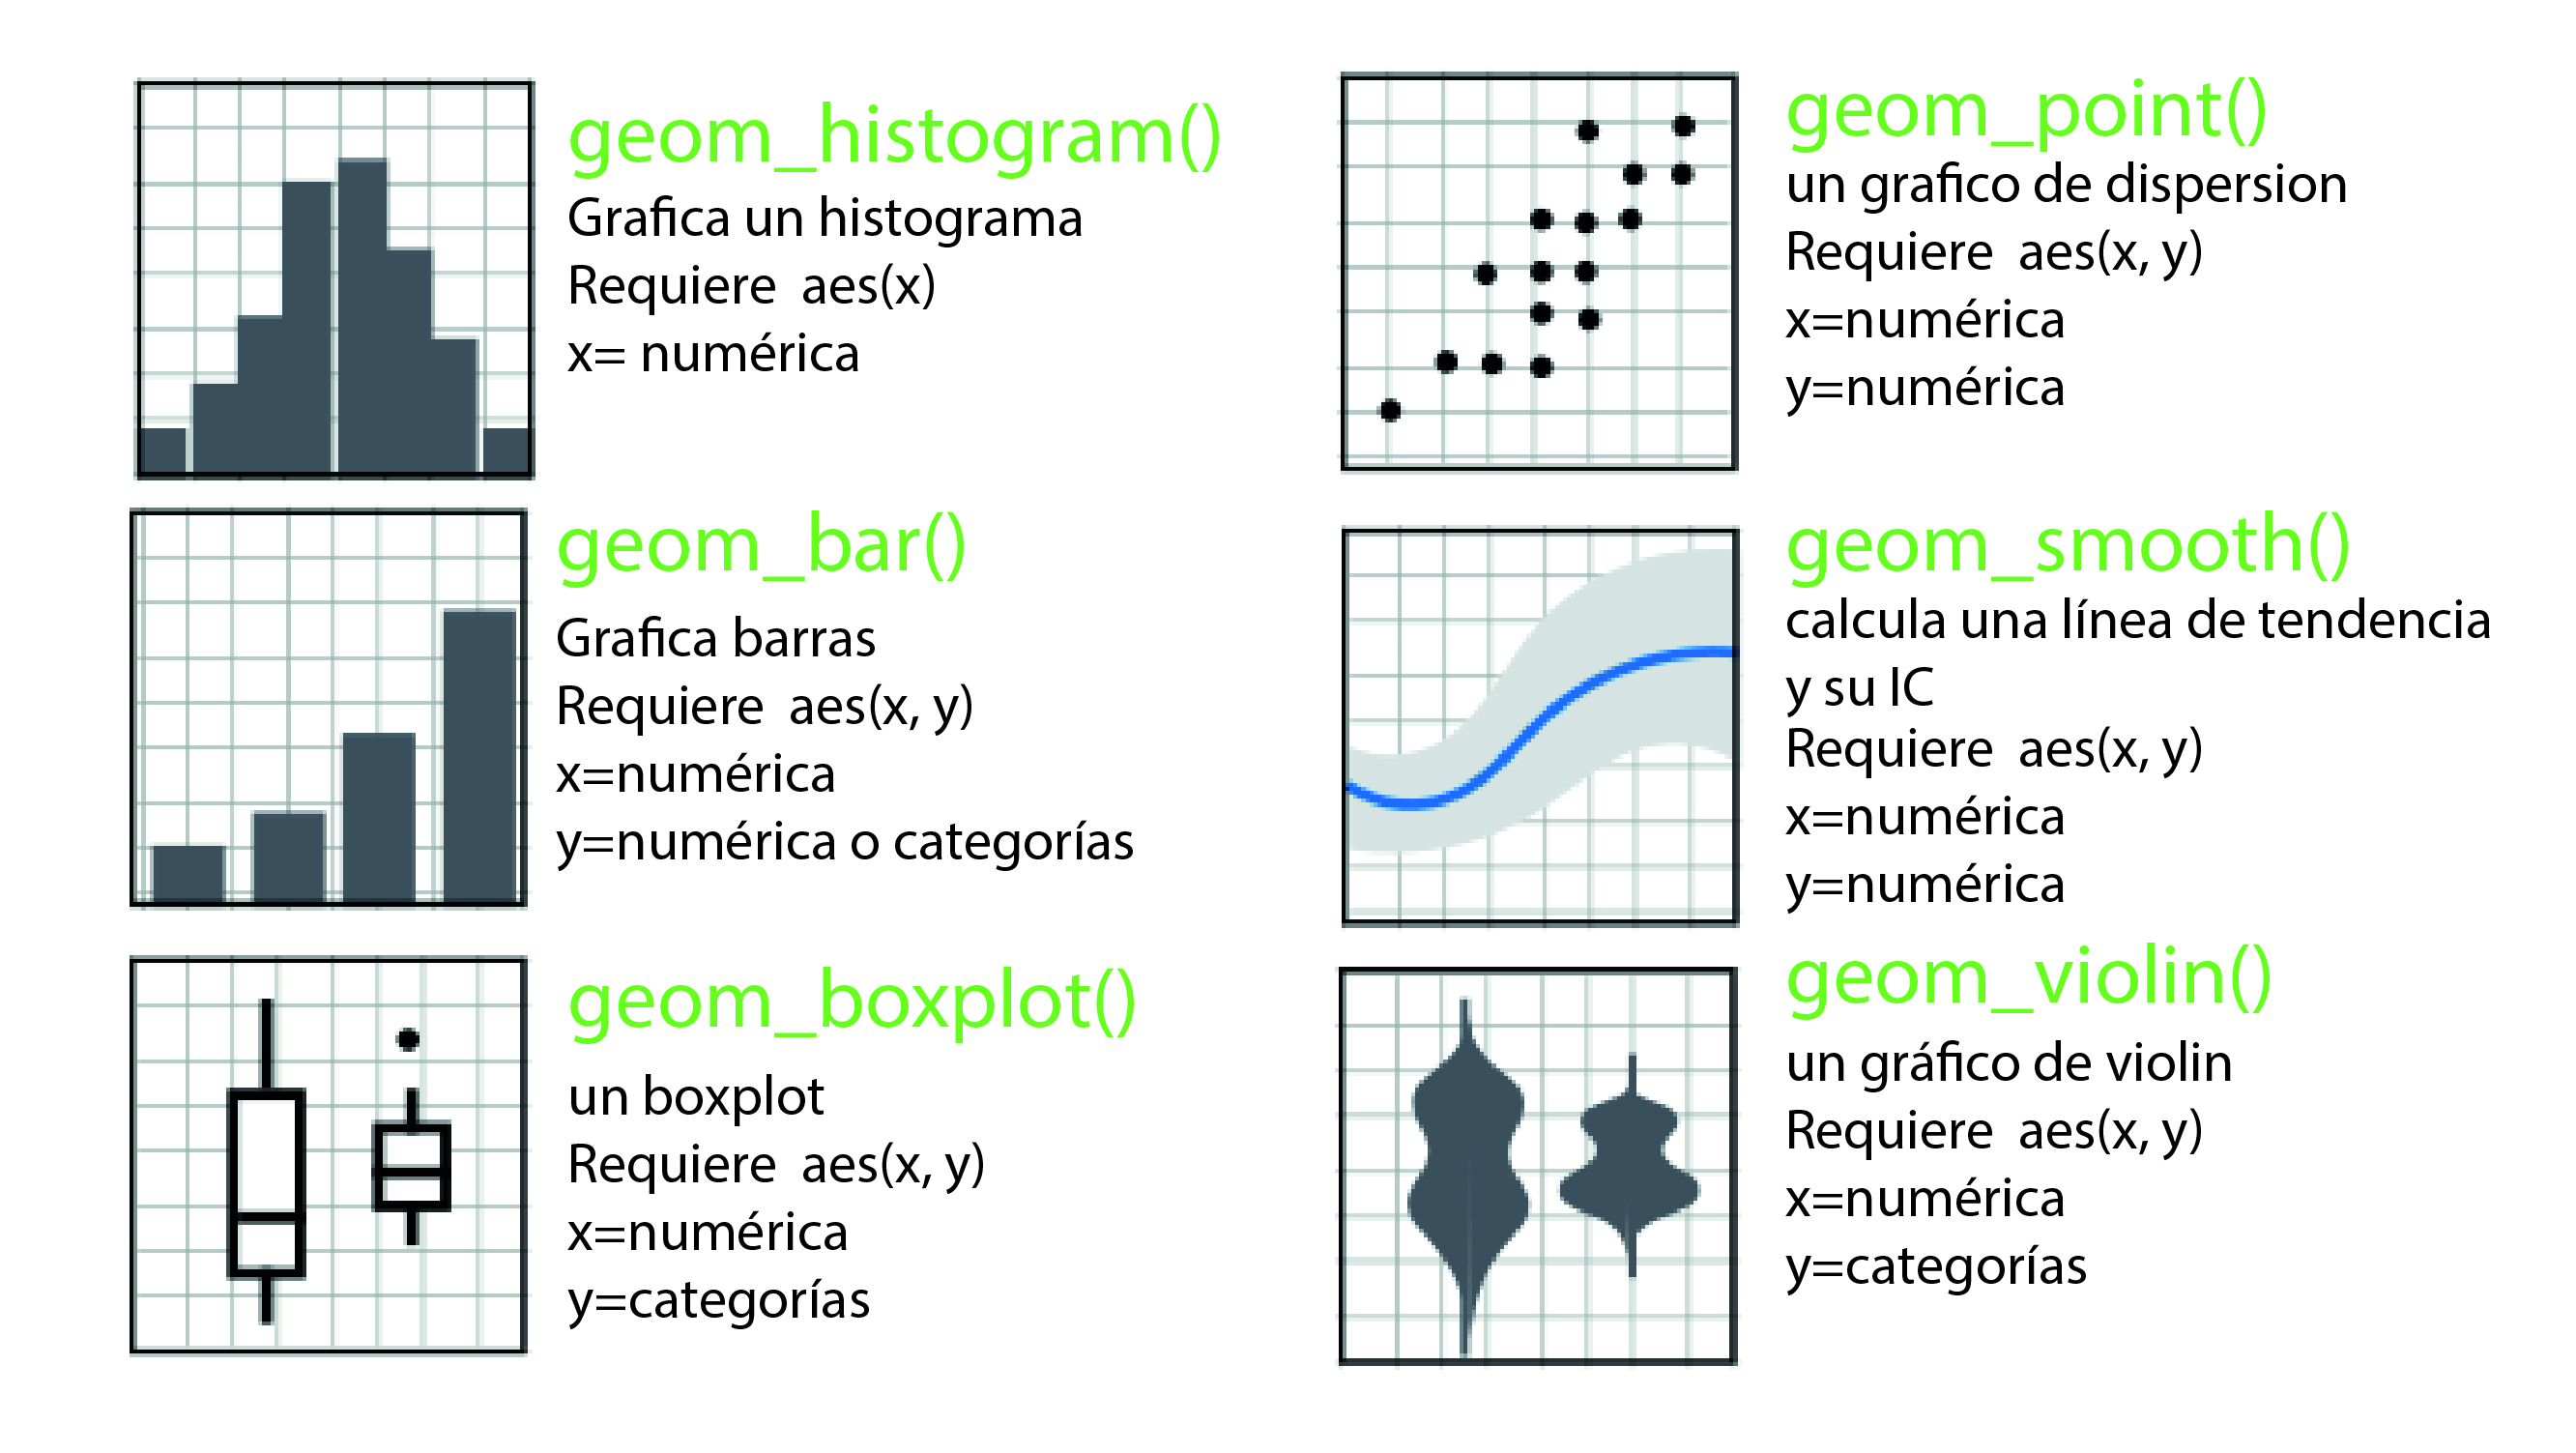
\includegraphics{./imgs/ggplot.jpg}

Dos cosas a destacar son que (como dijimos antes) ggplot no va a
graficar nada si no le decimos dónde están los datos ni los mapeamos (la
primera línea) y si no tiene una geometría. Como ven aquí entonces cada
geometría depende de que estén disponibles cierto tipo de datos en el
mapeo estético. Por ejemplo no puede crear una línea de tendencia si x e
y son categorías.

Hay muchísimas geometrías, los invito a que las exploren y busquen
cuáles son las que pueden funcionar mejor para cada uno de sus datos. Un
buen lugar para comenzar esta búsqueda es la
\href{https://r-graph-gallery.com/}{galería de gráficos de R}.

Habrán notado que cada capa de una geometría es una función, cada una
con sus propios argumentos, generalmente estos argumentos nos permiten
modificar la estética de esa geometría. Por ejemplo, en el caso de
\texttt{geom\_point} podemos modificar el tamaño de los puntos con el
argumento \texttt{size}, la transparencia con \texttt{alpha} o la forma
con \texttt{shape}. En el caso de \texttt{geom\_smooth} podemos elegir
el método de ajuste (por ejemplo, una línea de tendencia lineal) con el
argumento \texttt{method} o si queremos mostrar o no el intervalo de
confianza con \texttt{se}. Cada geometría tiene sus propios argumentos,
pero también hay argumentos comunes a todas las geometrías como
\texttt{color}, \texttt{fill}, \texttt{size}, etc.

\begin{tcolorbox}[enhanced jigsaw, breakable, rightrule=.15mm, colbacktitle=quarto-callout-tip-color!10!white, bottomtitle=1mm, arc=.35mm, titlerule=0mm, left=2mm, toprule=.15mm, leftrule=.75mm, colback=white, opacitybacktitle=0.6, opacityback=0, colframe=quarto-callout-tip-color-frame, bottomrule=.15mm, coltitle=black, toptitle=1mm, title=\textcolor{quarto-callout-tip-color}{\faLightbulb}\hspace{0.5em}{Mapeos en las geometrías}]
Habrán notado que \texttt{size} , \texttt{shape} o \texttt{alpha} (la
transparencia), son argumentos que mencionamos en la capa de mapeo
estético. También dijimos que pueden ser mapeos o parámetros fijos.
Bueno, el mapeo estético no es una función exclusiva de la primera capa,
puede ser un argumento dentro de una geometría, pero tenemos que saber
que \textbf{solamente} va a ser usada para esa geometría y no va a
afectar a las otras.

Para entenderlo mejor, si el mapeo estético se define en la primera
línea del gráfico (\texttt{ggplot()}), afecta a todas las geometrías. En
cambio, si se define dentro de una geometría específica
(\texttt{geom\_*()}), solo afecta a esa capa.

Veamos un ejemplo.

\begin{Shaded}
\begin{Highlighting}[]
\FunctionTok{ggplot}\NormalTok{(}
  \AttributeTok{data =}\NormalTok{ mtcars, }\CommentTok{\# 1. DATOS}
  \FunctionTok{aes}\NormalTok{(}\AttributeTok{x =}\NormalTok{ wt, }\CommentTok{\# 2. MAPEO ESTÉTICO}
      \AttributeTok{y =}\NormalTok{ mpg,}
      \AttributeTok{color =} \FunctionTok{factor}\NormalTok{(cyl))) }\SpecialCharTok{+}
  \FunctionTok{geom\_point}\NormalTok{(}\AttributeTok{alpha =} \FloatTok{0.7}\NormalTok{) }\SpecialCharTok{+} \CommentTok{\# 3. GEOMETRÍAS                }
  \FunctionTok{geom\_smooth}\NormalTok{(}\AttributeTok{method =} \StringTok{"lm"}\NormalTok{, }\AttributeTok{se =} \ConstantTok{FALSE}\NormalTok{) }\SpecialCharTok{+}
  \FunctionTok{theme\_minimal}\NormalTok{()                         }
\end{Highlighting}
\end{Shaded}

\begin{figure}[H]

{\centering 
\includegraphics[width=18.75in,height=\textheight]{./intro_R_files/figure-pdf/unnamed-chunk-31-1.pdf}

}

\end{figure}

En este caso, el mapeo estético de \texttt{color} está en la primera
línea por lo que afecta a la primera capa de geometrías
\texttt{geom\_point} y a la segunda \texttt{geom\_smooth} creando una
línea de tendencia por cada tipo de cilindrada a la que asigno un color

\begin{Shaded}
\begin{Highlighting}[]
\FunctionTok{library}\NormalTok{(ggplot2)}
\FunctionTok{ggplot}\NormalTok{(}
  \AttributeTok{data =}\NormalTok{ mtcars,}\CommentTok{\# 1. DATOS}
  \FunctionTok{aes}\NormalTok{(}\AttributeTok{x =}\NormalTok{ wt, }\CommentTok{\# 2. MAPEO ESTÉTICO}
      \AttributeTok{y =}\NormalTok{ mpg)) }\SpecialCharTok{+}
  \FunctionTok{geom\_point}\NormalTok{(}\AttributeTok{alpha =} \FloatTok{0.7}\NormalTok{, }\FunctionTok{aes}\NormalTok{(}\AttributeTok{color =} \FunctionTok{factor}\NormalTok{(cyl))) }\SpecialCharTok{+} \CommentTok{\# 3. GEOMETRÍAS           }
  \FunctionTok{geom\_smooth}\NormalTok{(}\AttributeTok{method =} \StringTok{"lm"}\NormalTok{, }\AttributeTok{se =} \ConstantTok{FALSE}\NormalTok{) }\SpecialCharTok{+}
  \FunctionTok{theme\_minimal}\NormalTok{()                         }
\end{Highlighting}
\end{Shaded}

\begin{figure}[H]

{\centering 
\includegraphics[width=18.75in,height=\textheight]{./intro_R_files/figure-pdf/unnamed-chunk-32-1.pdf}

}

\end{figure}

En esta versión en cambio el mapeo estético de color se encuentra dentro
de \texttt{geom\_point} (afecta solo a esta) dando lugar así a una única
línea en \texttt{geom\_smooth} (porque esa capa no tiene indicado un
mapeo de color).

Como ven, hay otros argumentos dentro de la geometría como \texttt{size}
dentro de + que son parámetros fijos del temeño de los puntos y no estan
ligados a ninguna variable
\end{tcolorbox}

\hypertarget{capas-adicionales}{%
\paragraph{Capas adicionales}\label{capas-adicionales}}

Una vez que hemos dominado la estructura de cimientos (data y mapeo
estético) y las capas de geometrías estamos en condiciones de generar la
gran mayoría de gráficos que necesitamos, pero las posibilidades de
\emph{\{ggplot2\}} son mucho mas amplias, hablaremos de capaz
adicionales que pueden mejorar mucho los resultados o enriquecen la
visualización.

\textbf{Escalas} Las escalas controlan cómo los valores se traducen en
colores, tamaños o transformaciones.

\begin{Shaded}
\begin{Highlighting}[]
\FunctionTok{scale\_color\_continuous}\NormalTok{()}
\CommentTok{\# Controla qué colores se usan para representar una variable numérica cuando esta está mapeada al color en el gráfico.}
\end{Highlighting}
\end{Shaded}

También pueden transformar los ejes:

\begin{Shaded}
\begin{Highlighting}[]
\FunctionTok{scale\_x\_log10}\NormalTok{()}
\end{Highlighting}
\end{Shaded}

Esto permite representar relaciones no lineales de forma más clara.

\textbf{Facetas}

Las facetas permiten dividir el gráfico en subgráficos según una
variable. Esto facilita comparar grupos.

Por ejemplo:

\begin{Shaded}
\begin{Highlighting}[]
\FunctionTok{facet\_wrap}\NormalTok{(}\SpecialCharTok{\textasciitilde{}}\NormalTok{ sexo)}
\CommentTok{\# Divide el gráfico inicial en uno para cada sexo}
\end{Highlighting}
\end{Shaded}

\textbf{Temas}

Los temas controlan la apariencia general:

\begin{itemize}
\item
  Fondo
\item
  Tipografía
\item
  Líneas
\item
  Grilla
\end{itemize}

Se pueden usar temas predefinidos como \texttt{theme\_minimal()} o
\texttt{theme\_classic()}, o personalizar cada elemento utilizando la
función \texttt{theme()}. Esta última permite controlar casi todos los
aspectos visuales del gráfico, desde el tamaño y estilo de las fuentes
hasta el color de fondo y las líneas de la grilla. Por ejemplo, podemos
modificar el título del gráfico, los títulos de los ejes, el color de
los valores de los ejes, las líneas principales de la grilla, etc.

Veamos un ejemplo:

\begin{Shaded}
\begin{Highlighting}[]
  \FunctionTok{theme}\NormalTok{(}
    \CommentTok{\# Modifica el título del gráfico}
    \AttributeTok{plot.title =} \FunctionTok{element\_text}\NormalTok{(}
      \AttributeTok{size =} \DecValTok{16}\NormalTok{,       }\CommentTok{\# Tamaño de la fuente}
      \AttributeTok{face =} \StringTok{"bold"}\NormalTok{,   }\CommentTok{\# Negrita}
      \AttributeTok{hjust =} \FloatTok{0.5}      \CommentTok{\# Centra el título (0 = izquierda, 1 = derecha)}
\NormalTok{    ),}
    
    \CommentTok{\# Cambia el tamaño de los títulos de los ejes}
    \AttributeTok{axis.title =} \FunctionTok{element\_text}\NormalTok{(}
      \AttributeTok{size =} \DecValTok{12}
\NormalTok{    ),}
    
    \CommentTok{\# Modifica el texto de los ejes (números)}
    \AttributeTok{axis.text =} \FunctionTok{element\_text}\NormalTok{(}
      \AttributeTok{color =} \StringTok{"darkred"}   \CommentTok{\# Color de los valores de los ejes}
\NormalTok{    ),}
    
    \CommentTok{\# Personaliza las líneas principales de la grilla}
    \AttributeTok{panel.grid.major =} \FunctionTok{element\_line}\NormalTok{(}
      \AttributeTok{color =} \StringTok{"gray80"}    \CommentTok{\# Color suave para mejorar legibilidad}
\NormalTok{    ),}
    
    \CommentTok{\# Elimina las líneas secundarias de la grilla}
    \AttributeTok{panel.grid.minor =} \FunctionTok{element\_blank}\NormalTok{(),}
    
    \CommentTok{\# Cambia el fondo del panel donde están los datos}
    \AttributeTok{panel.background =} \FunctionTok{element\_rect}\NormalTok{(}
      \AttributeTok{fill =} \StringTok{"white"}      \CommentTok{\# Fondo blanco del área del gráfico}
\NormalTok{    ),}
    
    \CommentTok{\# Cambia el fondo general del gráfico}
    \AttributeTok{plot.background =} \FunctionTok{element\_rect}\NormalTok{(}
      \AttributeTok{fill =} \StringTok{"gray95"}     \CommentTok{\# Color de fondo externo}
\NormalTok{    )}
\NormalTok{  )}
\end{Highlighting}
\end{Shaded}

\begin{tcolorbox}[enhanced jigsaw, breakable, rightrule=.15mm, colbacktitle=quarto-callout-tip-color!10!white, bottomtitle=1mm, arc=.35mm, titlerule=0mm, left=2mm, toprule=.15mm, leftrule=.75mm, colback=white, opacitybacktitle=0.6, opacityback=0, colframe=quarto-callout-tip-color-frame, bottomrule=.15mm, coltitle=black, toptitle=1mm, title=\textcolor{quarto-callout-tip-color}{\faLightbulb}\hspace{0.5em}{Capas adicionales y la grammar of graphics}]
No está de más recordar que la \emph{grammar of graphics} rige para
todas estas funciones y las reglas de adición son las mismas. Por
ejemplo:

\begin{Shaded}
\begin{Highlighting}[]
  \FunctionTok{theme}\NormalTok{(}
    \CommentTok{\# Modifica el texto de los ejes (números)}
    \AttributeTok{axis.text =} \FunctionTok{element\_text}\NormalTok{(}
      \AttributeTok{color =} \StringTok{"darkred"}   \CommentTok{\# Color de los valores de los ejes}
\NormalTok{    ))}\SpecialCharTok{+}
    \FunctionTok{theme\_minimal}\NormalTok{()}
\end{Highlighting}
\end{Shaded}

En este caso el tema minimalista se va a superponer al tema
personalizado en que cambiamos el color del texto del eje, por lo que el
resultado final va a ser un gráfico minimalista sin cambio en el color
de los valores de los ejes. Si queremos que el tema minimalista sea la
base y luego personalizarlo con nuestro tema personalizado, el orden de
las capas debe ser el opuesto.
\end{tcolorbox}

\hypertarget{instrucciones-finales-de-ggplot}{%
\subsubsection{Instrucciones finales de
ggplot}\label{instrucciones-finales-de-ggplot}}

El paquete \emph{\{ggplot2\}} es una herramienta muy versátil y poderosa
para la visualización de datos. La combinación de su estructura modular,
la amplia variedad de geometrías y la capacidad de personalización lo
convierten en una opción ideal para crear gráficos informativos y
atractivos. A medida que te familiarices con sus componentes y
funciones, vas a poder aprovechar al máximo su potencial para comunicar
tus datos y tus \emph{insights} de manera efectiva.

Sólo algunas recomendaciones antes de crear tus propios gráficos.
Recordá:

\begin{itemize}
\tightlist
\item
  definí claramente tus datos y mapeos estéticos;
\item
  elegí la geometría adecuada para tu tipo de datos y mensaje;
\item
  Personalizá tu gráfico con escalas, facetas y temas para mejorar la
  claridad y la estética;
\item
  \textbf{no te olvides de la lógica de capas}: el orden en que agregas
  las capas puede afectar el resultado final. Es fundamental pensar en
  términos de construcción progresiva;
\item
  \textbf{no confundas mapeos y parámetros}: Asegúrate de entender la
  diferencia entre mapeos estéticos (que dependen de las variables) y
  parámetros fijos (que son constantes). Esto es crucial para evitar
  confusiones en la interpretación de tus gráficos;
\item
  \textbf{asegurate que tus datos estén limpios y el tipo de variable
  bien definido}: \emph{\{ggplot2\}} es muy poderoso pero también es
  sensible a la calidad de los datos. Chequeá que tus datos estén
  limpios, sin valores faltantes o errores, y que las variables estén
  correctamente definidas (por ejemplo, factores para categorías). Esto
  va a facilitar que el mapeo estético y el gráfico final funcionen
  bien.
\end{itemize}

Si quieren saber más de \emph{\{ggplot2\}} les recomiendo
\href{https://www.cedricscherer.com/2019/08/05/a-ggplot2-tutorial-for-beautiful-plotting-in-r/}{este
hermoso tutorial} de uno de los gurúes de la visualización de datos con
\emph{\{ggplot2\}}, Cedric Scherer.

\hypertarget{algunas-palabras-finales}{%
\section{Algunas palabras finales}\label{algunas-palabras-finales}}

Como vimos brevemente en este capítulo, los paquetes del
\emph{tidyverse} son una herramienta importantísima para el análisis de
datos utilizando \textbf{R}. Para más detalles sobre estas
funcionalidades les recomendamos la guía de Hadley Wickham(Wickham
et~al.
2019)\marginpar{\begin{footnotesize}\leavevmode\vadjust pre{\protect\hypertarget{ref-wickham2019welcome}{}}%
Wickham, Hadley, Mara Averick, Jennifer Bryan, Winston Chang, Lucy
D'Agostino McGowan, Romain François, Garrett Grolemund, et~al. 2019.
{«Welcome to the Tidyverse»}. \emph{Journal of open source software} 4
(43): 1686.\vspace{2mm}\par\end{footnotesize}}
o, si ya se quieren sumergir de lleno en el mundo del análisis de datos
con R, este fantástico libro {[}Wickham, Çetinkaya-Rundel, y Grolemund
(2023)\marginpar{\begin{footnotesize}\leavevmode\vadjust pre{\protect\hypertarget{ref-wickham2023r}{}}%
Wickham, Hadley, Mine Çetinkaya-Rundel, y Garrett Grolemund. 2023.
\emph{R for data science}. " O'Reilly Media, Inc.".\vspace{2mm}\par\end{footnotesize}}{]}\sidenote{\footnotesize Disponible
  gratis online en \href{https://r4ds.had.co.nz/}{acá}.}.

\hypertarget{preguntas-de-repaso}{%
\section{Preguntas de repaso}\label{preguntas-de-repaso}}

\begin{enumerate}
\def\labelenumi{\arabic{enumi}.}
\item
  Tenés datos sobre performance en un juego de tres sujetos: Fran, Lu y
  Mateo. A cada uno, lo mediste tres veces, y en cada medición,
  registraste tiempo de reacción, tasa de respuestas correctas correcta
  y clicks.

  \begin{enumerate}
  \def\labelenumii{\alph{enumii})}
  \item
    ¿Cómo ordenarías estos datos para que estén en formato \emph{tidy}?
    (explicar cómo ordenarías las filas y columnas en una tabla)
  \item
    ¿Qué ventajas trae almacenar los datos en formato \emph{tidy}? ¿Qué
    desventajas trae?
  \item
    ¿Qué funciones se podrían utilizar para ordenar los datos de formato
    \emph{wide} a \emph{tidy} y viceversa?
  \end{enumerate}
\item
  ¿Qué significa que un dataset esté en formato \emph{tidy}?
\item
  ¿Cuál es la diferencia entre el formato tidy (o long) y el formato
  wide? Mencioná al menos una ventaja y una desventaja de almacenar los
  datos en formato tidy.
\item
  Explicá qué hace el operador pipe (\textbar\textgreater) y cuál es su
  utilidad
\item
  Describí para qué se usa cada uno de los siguientes verbos de
  \emph{\{dplyr\}}: \texttt{filter()}, \texttt{select()},
  \texttt{mutate()} y \texttt{summarise()}. ¿En qué se diferencia el
  resultado de usar \texttt{mutate()} en combinación con
  \texttt{group\_by()} del resultado de usar \texttt{summarise()} en
  combinación con \texttt{group\_by()}?
\item
  En el contexto del paquete \emph{\{ggplot2\}}, ¿que significa
  \emph{Grammar of Graphics}? ¿Cuáles son los elementos fundamentales de
  este sistema?
\item
  Supongamos que hacés un gráfico de dispersión con puntos utilizando
  funciones de \emph{\{ggplot2\}} y le agregás una línea de tendencia.
  Ves que algunos de los puntos que te interesan quedan tapados por la
  línea. ¿Qué puede estar pasando? ¿Cómo lo corregirías?
\end{enumerate}

\bookmarksetup{startatroot}

\hypertarget{sec-intro_stat}{%
\chapter{Repaso de probabilidad y estadística}\label{sec-intro_stat}}

Hola y bienvenidos a este repaso de probabilidad y estadística. En esta
sección vamos a repasar algunos conceptos básicos de probabilidad y
estadística que nos van a ser de vital importancia para lo que sigue. No
vamos a entrar en detalle\sidenote{\footnotesize Repetimos la recomendación. Si
  quieren profundizar en alguno de los temas pueden leer el capítulo 1
  de (Wasserman 2004) o el repaso de probabilidad de (Cunningham 2021)
  (disponible
  online).\linebreak\linebreak\leavevmode\vadjust pre{\protect\hypertarget{ref-wasserman2004all}{}}%
Wasserman, Larry. 2004. \emph{All of statistics: a concise course in
statistical inference}. Springer Science \& Business Media.\linebreak\linebreak\linebreak\leavevmode\vadjust pre{\protect\hypertarget{ref-cunningham2021causal}{}}%
Cunningham, Scott. 2021. \emph{Causal inference: The mixtape}. Yale
university press.\linebreak},
ni vamos a hacer demostraciones, sino que vamos a tratar de
\textbf{entender los conceptos de forma intuitiva y práctica}.

\hypertarget{eventos-aleatorios}{%
\section{Eventos aleatorios}\label{eventos-aleatorios}}

Un evento aleatorio es un resultado posible de un experimento aleatorio.
Por ejemplo, si tiramos una moneda al aire, los eventos aleatorios
posibles son ``cara'' y ``ceca''. Si tiramos dos monedas, los eventos
aleatorios posibles son ``cara-cara'', ``cara-ceca'', ``ceca-cara'' y
``ceca-ceca''. En general, el conjunto de todos los eventos aleatorios
posibles se llama espacio de eventos y se denota con la letra
\(\Omega\).

\hypertarget{variables-aleatorias}{%
\section{Variables aleatorias}\label{variables-aleatorias}}

Wasserman(Wasserman
2004)\marginpar{\begin{footnotesize}\leavevmode\vadjust pre{\protect\hypertarget{ref-wasserman2004all}{}}%
Wasserman, Larry. 2004. \emph{All of statistics: a concise course in
statistical inference}. Springer Science \& Business Media.\vspace{2mm}\par\end{footnotesize}}
nos dice que una variable aleatoria es un mapeo entre el espacio de
eventos y los números reales (\(X:\Omega \rightarrow \mathbb{R}\)).
Momento cerebrito ¿Esto que quiere decir? En términos prácticos, lo que
implica esta definición es que una variable aleatoria nos da un número
para cada evento del posible espacio de eventos aleatorios.

Vamos con un ejemplo que nos aclare un poco las cosas. Supongan que
tiramos una moneda justa\sidenote{\footnotesize Una moneda justa es aquella que tiene
  la misma probabilidad de dar cara o ceca, es decir,
  \(P(H) = P(T) = 0.5\).} dos veces y tenemos la variable aleatoria
\(X\) que cuenta la cantidad de caras (H)\sidenote{\footnotesize Cara será \textbf{H},
  del inglés \emph{Head} y ceca será \textbf{T}, del inglés \emph{Tail}.}.
Los posibles eventos \(\omega\) del espacio de eventos \(\Omega\) son
\(\Omega = \{ TT, TH, HT, HH \}\), es decir, que salga ceca y ceca, ceca
y cara, cara y ceca, y cara y cara. Uno podría pensar que la variable
aleatoria podría tomar un \(1\) para cara y un \(0\) para ceca, pero
recordemos la definición de la variable \(X\). Lo que nos interesa es la
cantidad de caras y es por eso que, en este caso, la variable aleatoria
\(X\) va a tomar los valores \(X = \{ 0, 1, 1, 2\}\), correspondientes a
cada evento aleatorio \(\omega \in \Omega\). Esto, en resumidas cuentas,
es lo que hace una variable aleatoria, convertir un evento aleatorio
(por ejemplo, \(HH\)) en un valor numérico (en este caso \(2\)).

En el ejemplo anterior \(X\) es lo que se denomina una variable
aleatoria discreta, es decir, que sólo puede tomar algunos valores
posibles (en este caso \(X = \{ 0, 1, 1, 2\}\)). Pero es importante
recordar que también existen variables aleatorias continuas como por
ejemplo la altura de una nueva persona que nace o la temperatura de
Buenos Aires en un día de enero 🥵.

Una pregunta que nos podemos hacer es: ¿para que nos interesa definir
una variable aleatoria si lo que queremos estudiar son los eventos
aleatorios? Bueno, porque traducir esos eventos (que pueden ser dos
tiradas de monedas o algo mucho más complejo, como tener o no tener una
enfermedad) en un número tiene grandes ventajas al momento de modelizar
la distribución de probabilidades.

\hypertarget{probabilidad}{%
\section{Probabilidad}\label{probabilidad}}

El concepto de probabilidad es algo complejo, pero, como esto no es un
curso de probabilidad, vamos a confiar en que ustedes ya lo tienen
claro. Si tienen coraje pueden ir a leer el capítulo 1 de (Wasserman
2004)\marginpar{\begin{footnotesize}\leavevmode\vadjust pre{\protect\hypertarget{ref-wasserman2004all}{}}%
Wasserman, Larry. 2004. \emph{All of statistics: a concise course in
statistical inference}. Springer Science \& Business Media.\vspace{2mm}\par\end{footnotesize}}
y, si quieren algo más terrenal, pueden ir a ver el repaso de
probabilidad de (Cunningham
2021)\marginpar{\begin{footnotesize}\leavevmode\vadjust pre{\protect\hypertarget{ref-cunningham2021causal}{}}%
Cunningham, Scott. 2021. \emph{Causal inference: The mixtape}. Yale
university press.\vspace{2mm}\par\end{footnotesize}}
(disponible online). Pero, de forma general, podemos decir que la
probabilidad es una medida numérica de la incertidumbre -o la certeza-
de que un evento aleatorio ocurra\sidenote{\footnotesize Existen dos grandes
  interpretaciones de la probabilidad: la frecuentista y la bayesiana.
  La primera define a la probabilidad como la frecuencia relativa de un
  evento en una serie de experimentos repetidos, mientras que la segunda
  la define como una medida subjetiva de la creencia o confianza en que
  un evento ocurra. Si quieren bucear en las profundas aguas de este
  debate pueden empezar por
  \href{https://www.youtube.com/watch?v=GEFxFVESQXc}{acá}.}.

Como dijimos que tenemos una moneda justa, es razonable pensar que todos
los eventos aleatorios en este espacio de eventos
\(\Omega = {TT, TH, HT, HH}\) son equiprobables, es decir, que cada uno
de ellos tiene la misma probabilidad de ocurrir, ¿no? Entonces, la
probabilidad de ocurrencia de cada evento será de \(1/4\)\sidenote{\footnotesize El
  enfoque frecuentista de la estadística justamente se basa en controlar
  los errores dada una repetición infinita de mi experimento.}. ¿Pero
podemos decir lo mismo de los posibles valores de \textbf{X}? ¿Tiene la
misma probabilidad de valer \(0\) que de valer \(1\)?

Como confío que son gente inteligente,y un poco ansiosa, ya deben haber
chusmeado esta tabla y se habrán dado cuenta que la respuesta es no.

\begin{longtable}[]{@{}ccc@{}}
\toprule()
\(\omega\) & \(X(\omega)\) & \(P({\omega})\) \\
\midrule()
\endhead
TT & 0 & 1/4 \\
TH & 1 & 1/4 \\
HT & 1 & 1/4 \\
HH & 2 & 1/4 \\
\bottomrule()
\end{longtable}

Lo que vemos es que hay dos eventos aleatorios (TH y HT) que se
``mapean'' al mismo valor de \textbf{X} (en este caso 1) y esto hace que
la probabilidad de que \textbf{X} tome el valor de 1 no sea de \(1/4\)
sino de \(1/2\).

Este bello y simplísimo ejemplo tiene el único objetivo de pensar un
poco para qué sirve una variable aleatoria y cómo es diferente de un
evento aleatorio. No vamos a entrar en más detalle.

Cuando las variables aleatorias son continuas la cosa se complica un
poco más ya que \(P(X=c)\) (por ejemplo, la probabilidad de que una
variable tome un valor dado) es \textbf{cero}. Esto lo vamos a repensar
un poco en la siguiente sección, cuando definamos lo que nos importa
para este libro: las funciones de densidad y de distribución.

\hypertarget{probabilidad-condicional}{%
\section{Probabilidad condicional}\label{probabilidad-condicional}}

La probabilidad condicional es la probabilidad de que ocurra un evento
\(A\) dado que ocurrió un evento \(B\) y se escribe como \(P(A|B)\).
Esta puede calcularse como:

\begin{equation}\protect\hypertarget{eq-prob_cond}{}{
P(A|B) = \frac{P(A \cap B)}{P(B)}
}\label{eq-prob_cond}\end{equation}

donde \(P(A \cap B)\) es la probabilidad de que \(A\) y \(B\) ocurran
juntos. Esta fórmula se puede entender fácilmente a partir de la
definición de probabilidad como frecuencia relativa. Si tenemos una
serie de experimentos repetidos, la probabilidad de que ocurra \(A\)
dado que ocurrió \(B\) es simplemente la proporción de veces que ambos
eventos ocurrieron juntos (\(P(AB)\)) sobre la proporción de veces que
ocurrió B(\(P(B)\)).

Pensemos en el ejemplo de tirar dos monedas justas. Supongamos que
queremos saber la probabilidad de que salga exactamente una cara (\(A\))
dado que salió al menos una cara (\(B\)). En este caso, \(P(A \cap B)\)
es la probabilidad de que salga exactamente una cara y al menos una
cara, lo cual es simplemente la probabilidad de que salga exactamente
una cara (\(P(X=1)\)), es decir, \(P(A \cap B) = P(HT) + P(TH) = 1/2\).
Por otro lado, \(P(B)\) es la probabilidad de que salga al menos una
cara (\(P(X=1)+(P(X=2)\)), lo cual es igual a
\(P(B) = P(HT) + P(TH) + P(HH) = 3/4\). Entonces, al reemplazar en la
fórmula tenemos que:

\begin{equation}\protect\hypertarget{eq-prob_cond_calculo}{}{
P(A|B) = \frac{P(A \cap B)}{P(B)} = \frac{1/2}{3/4} = \frac{2}{3}
}\label{eq-prob_cond_calculo}\end{equation}

Por ahora quedémonos con esta definición simple que será de vital
importancia para lo que sigue.

\hypertarget{probabilidad-total}{%
\section{Probabilidad total}\label{probabilidad-total}}

Imaginemos que queremos calcular la probabilidad de un evento B a partir
de su relación condicional con A. Para esto, debemos considerar la
probabilidad de que ocurra B tanto si A ocurre como si no. Al ponderar
cada uno de estos escenarios por la probabilidad de que ocurran (o no),
obtenemos lo que se denomina probabilidad total, la cual se expresa de
la siguiente forma\sidenote{\footnotesize Recordemos que \(\neg\) es el símbolo lógico
  de la negación.}:

\begin{equation}\protect\hypertarget{eq-test}{}{
P(B) = P(B|A) \times P(A) +  P(B|\neg A) \times P(\neg A)
}\label{eq-test}\end{equation}

Pensemos un ejemplo. Imaginemos que una persona tiene que completar un
trabajo de jardinería (evento \(B\)) en un día. La probabilidad de que
termine este trabajo si llueve (evento \(A\)) es \(0.35\) y la
probabilidad de que lo termine si no llueve es de \(0.95\). Si la
probabilidad de que llueva es \(P(A)= 0.4\), ¿cuál es la probabilidad
(\(P(B)\)) de que el trabajo se complete en un día? Echemos mano a la
fórmula de probabilidad total:

\begin{equation}\protect\hypertarget{eq-probTotalEj}{}{
\begin{array}
_P(B) &=& P(B|A) \times P(A) + P(B|\neg A) \times P(\neg A) \\
&=& 0.35 \times 0.4 + 0.95 \times 0.6 \\
&=& 0.71
\end{array}
}\label{eq-probTotalEj}\end{equation}

Entonces, la probabilidad de completar el trabajo en un día es
\(P(B)=0.71\).

Por último, cuando tenemos muchas condiciones, podemos definir de forma
general a la probabilidad total como:

\begin{equation}\protect\hypertarget{eq-proba_total_1}{}{
P(B) = \sum_n P(B|A_n) P(A_n)
}\label{eq-proba_total_1}\end{equation}

🎩¡Matemagia!🎩

Ya que estamos cancheros, supongamos que tenemos el evento \(A_1\) y
queremos calcular su probabilidad condicional dado que ocurrió el evento
\(B\). Recordemos la definición de probabilidad condicional:

\begin{equation}\protect\hypertarget{eq-proba_total_2}{}{
P(A_1|B) = \frac{P(A_1 \cap B)}{P(B)}
}\label{eq-proba_total_2}\end{equation}

Pero también \(P(A_1|B)\) se puede escribir como

\begin{equation}\protect\hypertarget{eq-proba_total_3}{}{
P(B|A_1) = \frac{P(B \cap A_1)}{P(A_1)}
}\label{eq-proba_total_3}\end{equation}

Y como las intersecciones son iguales
(\(P(A_1 \cap B) = P(B \cap A_1)\), podemos despejar de la
Ecuación~\ref{eq-proba_total_3} a \(P(A_1 B) = P(B|A_1) P(A_1)\) y
reemplazarlo en la fórmula de probabilidad condicional:

\begin{equation}\protect\hypertarget{eq-proba_total_4}{}{
P(A_1|B) = \frac{P(A_1 \cap B)}{P(B)} = \frac{P(B|A_1) P(A_1)}{P(B)}
}\label{eq-proba_total_4}\end{equation}

Pero si recordamos la fórmula de probabilidad total
(Ecuación~\ref{eq-proba_total_1}), se puede reemplazar como:

\begin{equation}\protect\hypertarget{eq-proba_total_5}{}{
P(A_1|B) = \frac{P(B|A_1) P(A_1)}{\sum_{i=1}^n P(B|A_i) P(A_i)}
}\label{eq-proba_total_5}\end{equation}

Y de forma general:

\[
P(A_i|B) = \frac{P(B|A_i) P(A_i)}{\sum_{j=1}^n P(B|A_j) P(A_j)}
\]

Esto que acabamos de deducir es nada más ni nada menos que la fórmula de
Bayes, una de las fórmulas más importantes de la probabilidad y la
estadística. La fórmula de Bayes nos permite invertir la condicionalidad
de una probabilidad, es decir, calcular \(P(A/B)\) a partir de
\(P(B/A)\).

\hypertarget{teorema-de-bayes}{%
\section{Teorema de Bayes}\label{teorema-de-bayes}}

Ahora que ya llegamos a la fórmula de Bayes -a partir de las
definiciones de probabilidad total- podemos tomar prestado un ejemplo de
(Herzog, Francis, y Clarke
2019)\marginpar{\begin{footnotesize}\leavevmode\vadjust pre{\protect\hypertarget{ref-herzog2019understanding}{}}%
Herzog, Michael H, Gregory Francis, y Aaron Clarke. 2019.
\emph{Understanding statistics and experimental design: how to not lie
with statistics}. Springer Nature.\vspace{2mm}\par\end{footnotesize}}:
Tenemos un test para identificar si somos portadores de un virus
(llamémoslo IKV). Este test tiene una sensibilidad del 99.99\% y una
especificidad del 99.99\%. Es decir, la probabilidad de que el test de
positivo, dado que tenemos el virus (\(P(T^+|IKV)\)) es de 0.9999, y lo
mismo ocurre para la probabilidad de que el test de negativo en caso de
que \textbf{NO} tengamos el virus (\(P(T^-|\neg IKV)\)). Sabemos también
que la incidencia del virus IKV es de 1 en 10000.

Supongamos que somos elegidos \textbf{aleatoriamente} para realizarnos
el test y este da positiv: ¿qué probabilidad hay de ser portadores del
virus (\(P(IKV|T^+)\))? La primera respuesta que se nos viene es 0.9999
¿verdad?. Pero, si estuvimos prestando atención, ya a esta altura
debemos saber que para invertir la condicionalidad de una probabilidad
tenemos que acudir al bueno de Bayes (de la sensibilidad \(P(T^+|IKV)\)
a la que nos interesa \(P(IKV|T^+)\)). O sea:

\begin{equation}\protect\hypertarget{eq-test}{}{
P(IKV|T^+) = \frac{P(T^+|IKV) \times P(IKV)}{P(T+)}
}\label{eq-test}\end{equation}

donde \(P(T^+|IKV) = 0.9999\) y \(P(IKV) = 1/10000 = 0.0001\). Además,
echando mano a la definición de probabilidad total podemos calcular
\(P(T+)\) como:

\begin{equation}\protect\hypertarget{eq-test}{}{
P(T+) = P(T^+|IKV) \times P(IKV) + P(T^+|\neg IKV) \times P(\neg IKV)
}\label{eq-test}\end{equation}

donde \(P(T^+|\neg IKV) = 1-0.9999\) y \(P(\neg IKV) = 1-0.0001\). Al
reemplazar todos los valores tenemos que:

\begin{equation}\protect\hypertarget{eq-test}{}{
\begin{array}
_P(IKV|T^+) &=& \frac{P(T^+|IKV) \times P(IKV)}{P(T+)}\\
&=& \frac{P(T^+|IKV) \times P(IKV)}{P(T^+|IKV) \times P(IKV) + P(T^+|\neg IKV) \times P(\neg IKV)} \\
&=& \frac{0.9999 \times 0.0001}{0.9999 \times 0.0001 + (1-0.9999) \times (1-0.0001)} \\
&=& \frac{0.9999 \times 0.0001}{0.9999 \times 0.0001 + 0.0001 \times 0.9999} \\
&=& 0.5
\end{array}
}\label{eq-test}\end{equation}

¿Qué? ¿Esto significa que si el test me da positivo \textbf{sólo} tengo
un 0.5 de probabilidad de tener el virus? ¿Esto quiere decir que los
tests no sirven para nada? Momento, analicemos un poco el resultado al
que llegamos. Lo que nos dice esta cuenta es que, una vez que el test
nos da positivo, a pesar de lo sensible del test y por lo ``raro'' de la
portación del virus, nuestra probabilidad de ser portadores es de 0.5.
Pero, ¿y nuestra probabilidad de ser portadores si el test nos da
negativos? Hagamos la cuenta:

\begin{equation}\protect\hypertarget{eq-test}{}{
\begin{array}
_P(IKV|T^-) &=& \frac{P(T^-|IKV) \times P(IKV)}{P(T-)}\\
&=& \frac{P(T^-|IKV) \times P(IKV)}{P(T^-|IKV) \times P(IKV) + P(T^-|\neg IKV) \times P(\neg IKV)} \\
&=& \frac{(1-0.9999) \times 0.0001}{(1 - 0.9999) \times 0.0001 + (0.9999) \times (1-0.0001)} \\
&=& 1E-8
\end{array}
}\label{eq-test}\end{equation}

OK, ahora la cosa tiene más sentido. O sea, el test es bastante bueno
para decirnos cuando no somos portadores y dando negativo, el problema
es cuando da positivo. En este caso tenemos que preocuparnos, pero, como
vimos anteriormente, la probabilidad de ser portadores es de apenas 0.5.

Hay una solución más simple para esto y es la que deben estar pensando
ustedes: ¿Y si me hacen un segundo test? ¡BINGO 🎊! Calculemos
rápidamente la probabilidad de estar infectados si nos testean por
segunda vez:

\begin{equation}\protect\hypertarget{eq-test}{}{
P(IKV|T^{2+}) = \frac{0.9999^2 \times 0.0001}{0.9999^2 \times 0.0001 + 0.0001^2 \times 0.9999} = 0.9999
}\label{eq-test}\end{equation} Ahora sí, si somos testeados por segunda
vez, la probabilidad de ser portadores dado que tenemos dos resultados
positivos trepa a 0.9999. Nos podemos quedar tranquilos.

Para cerrar, me gustaría que pensemos un poco en una palabra MUY
importante que se dijo en el enunciado del problema:
\textbf{aleatoriamente}. En muchos de los casos en los que nos testeamos
para ver si somos portadores de un virus, lo hacemos porque tenemos
algún tipo de presunción de que podemos serlo (por ejemplo, tenemos
síntomas). ¿Cuál creen que sería la probabilidad que se modifica en la
fórmula? Exacto, \(P(IKV)\), ya que sería más bien \(P(IKV|síntomas)\).

Ahora metamos un volantazo y hablemos un poco de las variables
aleatorias y cómo medirlas y caracterizarlas.

\hypertarget{esperanza}{%
\section{Esperanza}\label{esperanza}}

La esperanza de una variable aleatoria \(X\), a veces también denominada
media poblacional, es simplemente la suma pesada de todos sus valores
posibles. No debemos confundir la esperanza con el promedio muestral,
aunque, como veremos en breve, para algunos casos este último es un
\textbf{estimador insesgado de la esperanza}.

La esperanza de una variable aleatoria discreta se define como:

\begin{equation}\protect\hypertarget{eq-test}{}{
E(X) = \sum_{1}^\infty x_i p(x_i)
}\label{eq-test}\end{equation}

En este caso es muy claro la naturaleza de promedio pesado, ya que a
cada valor posible de \(X\) lo estamos pesando por su probabilidad. Sin
embargo, para una variable aleatoria continua, en la que no tenemos
definida una probabilidad puntual \(p(x_i)\) sino una función de
densidad \(f(x)\)\sidenote{\footnotesize La función de densidad \(f(x)\) es una
  función que describe la distribución de probabilidad de una variable
  aleatoria continua. La probabilidad de que la variable tome un valor
  dentro de un intervalo se calcula integrando la función de densidad
  sobre ese intervalo.}, la definición es la siguiente:

\begin{equation}\protect\hypertarget{eq-test}{}{
E(X) = \int_{-\infty}^\infty x f(x) dx
}\label{eq-test}\end{equation}

Como resulta esperable, la suma se transforma en una integral y la
probabilidad puntual se reemplaza por \(f(x)\).

Algunas propiedades importantes de la esperanza son:

\begin{equation}\protect\hypertarget{eq-test}{}{
\begin{array}
_E(aX+b) & = & aE(X) + b\\
E(\sum_{i=1}^n X_i) & = & \sum_{i=1}^nE(X_i)
\end{array}
}\label{eq-test}\end{equation}

Por último, y a modo de aviso, advertencia y amenaza, recordemos que
\(E(X)^2 \neq E(X^2)\).

\hypertarget{varianza-y-covarianza}{%
\section{Varianza y covarianza}\label{varianza-y-covarianza}}

La varianza nos da una idea acerca de la variabilidad de los procesos
aleatorios que generan una variable aleatorio\sidenote{\footnotesize Dato que será de
  vital importancia para sentar las bases de la inferencia estadística.}.
La varianza de la variable aleatoria \(X\) se define como:

\begin{equation}\protect\hypertarget{eq-test}{}{
V(X) = \sigma^2 = E \left[ (X - E(X))^2 \right]
}\label{eq-test}\end{equation}

Y se puede demostrar que:

\begin{equation}\protect\hypertarget{eq-test}{}{
V(X) = E(X^2) - E^2(X)
}\label{eq-test}\end{equation}

Por otro lado, la covarianza mide la cantidad de dependencia lineal
entre dos variables aleatorias. Esta se define como

\begin{equation}\protect\hypertarget{eq-test}{}{
Cov(X,Y) = E(XY) - E(X)E(Y)
}\label{eq-test}\end{equation}

Si \(Cov(X,Y)>0\), esto indica que las dos variables se mueven en la
misma dirección, mientras que si \(Cov(X,Y)<0\) esto indica que ambas
variables se mueven en direcciones opuestas.

\hypertarget{correlaciuxf3n}{%
\section{Correlación}\label{correlaciuxf3n}}

Ahora una pregunta: ¿podemos comparar la covarianza de dos pares de
variables? Por ejemplo, si \(Cov(X, Y) = 14.988\) y
\(Cov(W, Z) = 0.001\), ¿podemos decir que \textbf{X} e \textbf{Y} están
más relacionadas que \textbf{W} y \textbf{Z}? La respuesta es no, ya que
la covarianza depende de la varianza de cada una de las variables, es
decir, de la escala en la que se midan. Esto hace que la covarianza no
sea una medida muy informativa para comparar la relación entre dos pares
de variables. Para poder hacer esta comparación vamos a tomar el camino
de la parsimonia y vamos a hacer lo que cualquier ser humano con
\emph{Estadística II} aprobada haría: normalizar la covarianza
dividiéndola por las varianzas de cada una de las variables. Esto se
llama \textbf{correlación} y nos dice cuánto covarían dos variables
independizándose de la varianza de cada una de ellas. Esto la convierte
en una medida muy relevante e informativa.

Si tenemos dos variables aleatorias \textbf{X} e \textbf{Y}, la
correlación se define como la covarianza de sus versiones
estandarizadas:

\begin{equation}\protect\hypertarget{eq-test}{}{
\begin{array}
_W &=& \frac{X-E(X)}{\sqrt{V(X)}} \\
Z &=& \frac{Y-E(Y)}{\sqrt{V(Y)}}
\end{array}
}\label{eq-test}\end{equation}

De la siguiente forma:

\begin{equation}\protect\hypertarget{eq-test}{}{
\begin{array}
_Corr(X,Y) &=& Cov(W,Z) \\
&=&  Cov(\frac{X-E(X)}{\sqrt{V(X)}}, \frac{Y-E(Y)}{\sqrt{V(Y)}}) \\
&=&  \frac{1}{\sqrt{V(X)}} \frac{1}{\sqrt{V(Y)}}  Cov(X-E(X),Y-E(Y)) \\
&=&  \frac{Cov(X,Y)}{\sqrt{V(X) V(Y)}}
\end{array}
}\label{eq-test}\end{equation}

Usamos la propiedad de la covarianza que dice que:

\begin{equation}\protect\hypertarget{eq-test}{}{
Cov(X+a, Y+b) = Cov(X,Y) + Cov(X,b) + Cov(a,Y) + Cov(a,b)
}\label{eq-test}\end{equation}

Y como \(a\) y \(b\) son constantes (en nuestro caso esperanzas), el
único término que sobrevive es \(Cov(X,Y)\). Esta magnitud también es
conocida como el coeficiente de correlación \(\rho\).

Con esta definición en la mano, si yo les digo que dos variables \(X\) e
\(Y\) tienen una covarianza de \(14.988\) no les dice mucho, ¿No? Ahora,
si les digo que el coeficiente de correlación es de \(0.788\)
probablemente entiendan rápidamente que ambas variables están muy
relacionadas\sidenote{\footnotesize Si quieren divertirse, y de paso convertirse en
  ases de la determinación del coeficiente de correlación a
  \emph{ojímetro}, les recomiendo
  \href{https://www.guessthecorrelation.com/}{este juegazo}. Una
  estudiante ostenta el abultado récord de \(231\) puntos ¿La pasaste?}.

Veamos este ejemplo con números y de paso repasemos cómo se calcula la
correlación en R:

\begin{Shaded}
\begin{Highlighting}[]
\FunctionTok{set.seed}\NormalTok{(}\DecValTok{1234}\NormalTok{)}
\NormalTok{x }\OtherTok{=} \FunctionTok{rnorm}\NormalTok{(}\DecValTok{1000}\NormalTok{, }\DecValTok{20}\NormalTok{, }\DecValTok{4}\NormalTok{)}
\NormalTok{y }\OtherTok{=}\NormalTok{ x}\SpecialCharTok{*}\NormalTok{.}\DecValTok{9} \SpecialCharTok{+} \FunctionTok{rnorm}\NormalTok{(}\DecValTok{1000}\NormalTok{, }\DecValTok{2}\NormalTok{, }\DecValTok{3}\NormalTok{)}
\FunctionTok{cat}\NormalTok{(}\FunctionTok{paste}\NormalTok{(}\StringTok{"La covarianza entre X e Y es"}\NormalTok{, }\FunctionTok{round}\NormalTok{(}\FunctionTok{cov}\NormalTok{(x,y), }\DecValTok{3}\NormalTok{)))}
\CommentTok{\#\textgreater{} La covarianza entre X e Y es 14.988}
\FunctionTok{cat}\NormalTok{(}\FunctionTok{paste}\NormalTok{(}\StringTok{"La correlación entre X e Y es"}\NormalTok{, }\FunctionTok{round}\NormalTok{(}\FunctionTok{cor}\NormalTok{(x,y), }\DecValTok{3}\NormalTok{)))}
\CommentTok{\#\textgreater{} La correlación entre X e Y es 0.788}
\end{Highlighting}
\end{Shaded}

\begin{figure}

{\centering 
\includegraphics[width=18.75in,height=\textheight]{./intro_stat_files/figure-pdf/unnamed-chunk-3-1.pdf}

}

\caption{Relación lineal entre X e Y.}

\end{figure}

Es muy importante tener en cuenta que el coeficiente de correlación nos
dice cuán \textbf{linealmente} relacionadas están las variables. Veamos
esto con un ejemplito:

\begin{Shaded}
\begin{Highlighting}[]
\FunctionTok{set.seed}\NormalTok{(}\DecValTok{1234}\NormalTok{)}
\NormalTok{x }\OtherTok{=} \FunctionTok{runif}\NormalTok{(}\DecValTok{1000}\NormalTok{, }\SpecialCharTok{{-}}\DecValTok{1}\NormalTok{, }\DecValTok{1}\NormalTok{)}
\NormalTok{y }\OtherTok{=}\NormalTok{ x}\SpecialCharTok{\^{}}\DecValTok{2} \SpecialCharTok{+}\NormalTok{ .}\DecValTok{1}\SpecialCharTok{*}\FunctionTok{runif}\NormalTok{(}\DecValTok{1000}\NormalTok{, }\SpecialCharTok{{-}}\DecValTok{1}\NormalTok{, }\DecValTok{1}\NormalTok{)}
\FunctionTok{cat}\NormalTok{(}\FunctionTok{paste}\NormalTok{(}\StringTok{"La covarianza entre X e Y es"}\NormalTok{, }\FunctionTok{round}\NormalTok{(}\FunctionTok{cov}\NormalTok{(x,y), }\DecValTok{3}\NormalTok{)))}
\CommentTok{\#\textgreater{} La covarianza entre X e Y es 0.01}
\FunctionTok{cat}\NormalTok{(}\FunctionTok{paste}\NormalTok{(}\StringTok{"La correlación entre X e Y es"}\NormalTok{, }\FunctionTok{round}\NormalTok{(}\FunctionTok{cor}\NormalTok{(x,y), }\DecValTok{3}\NormalTok{)))}
\CommentTok{\#\textgreater{} La correlación entre X e Y es 0.055}
\end{Highlighting}
\end{Shaded}

\begin{figure}

{\centering 
\includegraphics[width=18.75in,height=\textheight]{./intro_stat_files/figure-pdf/unnamed-chunk-5-1.pdf}

}

\caption{Relación no lineal entre X e Y.}

\end{figure}

En este caso vemos que claramente hay una relación entre \textbf{X} e
\textbf{Y} (no son una nube de puntos sin estructura), pero como esta
relación no es lineal (cuadrática en nuestro caso), el coeficiente de
correlación es cercano a cero.

Finalmente, tengamos en cuenta que el coeficiente de correlación puede
tomar valores entre \(-1\) y \(1\). Una correlación positiva indica que
las variables varían de la misma manera (si aumenta una aumenta la otra)
y lo contrario ocurre con una correlación negativa (si aumenta una
disminuye la otra). Cuanto más cerca esté el coeficiente de \(1\) o, más
fuerte es la relación lineal.

\hypertarget{poblaciuxf3n-y-muestra}{%
\section{Población y muestra}\label{poblaciuxf3n-y-muestra}}

Veamos la siguiente figura. En ella podemos ver cómo hay una
``población''\sidenote{\footnotesize Si bien podemos pensar en la población como el
  conjunto completo de individuos (u objetos o eventos) sobre los cuales
  se desea obtener información, creo que pensar en el proceso de
  generación de datos es una forma un poco más completa. Hagamos un
  pequeño ejercicio mental: si yo les preguntara cuál es el talle de
  zapatillas promedio de un estudiante de la Universidad de San Andrés.
  ¿Ustedes creen que la respuesta ``poblacional'' es medir el pie de
  todos los estudiantes que están este año en la universidad y calcular
  el promedio? Probablemente no, ya que esto es algo imposible de hacer.
  Lo que realmente queremos es conocer el proceso de generación de
  datos, es decir, la función de densidad que nos permita describir cómo
  se generan los datos (en este caso, la altura del pie de los
  estudiantes). Esto es lo que nos va a permitir hacer inferencias sobre
  la población a partir de una muestra.} de la que queremos saber algo.
La teoría de probabilidad nos ayuda a ``modelar'' esta población(es
decir, a definir una función de densidad que nos permita describir la
generación de los datos). La inferencia estadística, por otro lado, nos
ayuda a estimar los parámetros de esta función de densidad a partir de
una muestra de datos. Por supuesto, en estas estimaciones hay
aleatoriedad y si tomamos distintas muestras los resultados van a ser
diferentes. Es aquí (o acá) donde entra la inferencia estadística, para
ayudarnos a medir (o estimar) esta variabilidad y así poder cuantificar
la confianza que tenemos en las conclusiones sobre la población a partir
de la muestra.

\begin{figure}

{\centering 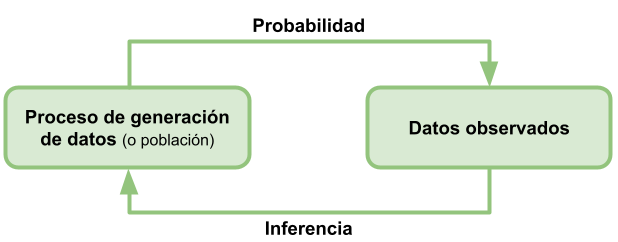
\includegraphics[width=6.25in,height=\textheight]{./imgs/probabilidad_e_inferencia.png}

}

\caption{Probabilidad e inferencia.}

\end{figure}

Vamos con un ejemplo que nos puede ayudar a entender de qué hablamos
cuando hablamos de estimación. Supongamos que conocemos la distribución
de la altura de la población de varones en Argentina (o sea, conocemos
el proceso de generación de datos\sidenote{\footnotesize Está de más decir que
  \textbf{nunca} vamos a conocer esto, o que si lo conociéramos no
  estaríamos pensando en hacer inferencia ni estimar nada.}). No estamos
hablando de calcular el promedio de la altura de los varones, sino de
que conocemos la función de densidad enla cual la altura de cada varón
es una muestra. Si no queda del todo claro respiren hondo y esperen un
poco que ya se va a ir aclarando. Entonces, la altura de los varones de
Argentina tiene una distribución normal\sidenote{\footnotesize Como dijimos
  anteriormente, este no es un libro de probabilidad, así que si no
  saben lo que es la distribución normal pueden ir a leerlo a sus
  apuntes de estadística (procede a preguntarle a ChatGPT ``¿Qué es la
  distribución normal?'').} con media en cm. de \(\mu_{varones} = 175\)
y una desviación estándar \(\sigma_{varones} = 7\), o, como ya
aprendimos a decir:
\(H_{varones} \sim \mathcal{N}(\mu_{varones},\sigma^2_{varones}) = \mathcal{N}(175, 49)\)\sidenote{\footnotesize \textbf{h}
  del inglés \emph{height}.}. A continuación podemos ver la función de
densidad:

\begin{figure}

{\centering 
\includegraphics[width=18.75in,height=\textheight]{./intro_stat_files/figure-pdf/unnamed-chunk-6-1.pdf}

}

\caption{Función de densidad de probabilidad de la variabla aleatoria H
(altura de los varones)}

\end{figure}

Ahora bien, en la figura podemos ver la función \(f_X(x)\) junto con una
línea vertical que nos indica la media y dos líneas que nos indican los
percentiles \(2.5\) y \(97.5\), es decir, que contienen el 95\% de la
masa de probabilidad. Todo esto es muy lindo pero estamos jugando a ser
dios (o el Doctor Manhattan, o en lo que ustedes crean). Es imposible
conocer los parámetros de esta distribución, pero lo que sí podemos
hacer en la práctica es estimarlos. Estimar los parámetros de un modelo
es \emph{el pan y la manteca} de la inferencia estadística y el
\emph{data mining}. Como podemos ver en esta hermosa figura de
Wasserman(Wasserman
2004)\marginpar{\begin{footnotesize}\leavevmode\vadjust pre{\protect\hypertarget{ref-wasserman2004all}{}}%
Wasserman, Larry. 2004. \emph{All of statistics: a concise course in
statistical inference}. Springer Science \& Business Media.\vspace{2mm}\par\end{footnotesize}},
la teoría de probabilidad nos ayuda a definir modelos para la generación
de datos y la inferencia estadística nos ayuda a estimar los parámetros
esos parámetros.

Hay diversas formas de encontrar estimadores para los parámetros de un
modelo (por ejemplo, método de los momentos, máxima verosimilitud, etc.)
pero entenemos que eso excede los contenidos de este curso. Sin embargo,
para estimar todos conocemos los estimadores de los parámetros
poblacionales \(\mu\) y \(\sigma^2\). Claro, el promedio \(\bar{x}\) y
el desvío muestral \(\hat{S}^2\):

\begin{equation}\protect\hypertarget{eq-test}{}{
\begin{array}
\\\bar{x} & = & n^{-1} \sum_{i=1}^n x_i\\
\hat{S}^2 & = & (n-1)^{-1} \sum_{i=1}^n (x_i 
\end{array}
}\label{eq-test}\end{equation}

Simulemos tres experimentos tomando 10, 50 y 100 mediciones (\(n\)) y
veamos los histogramas de estas muestras y sus estimaciones de \(\mu\) y
\(\sigma\):

\begin{figure}

{\centering 
\includegraphics[width=25in,height=\textheight]{./intro_stat_files/figure-pdf/unnamed-chunk-7-1.pdf}

}

\caption{Distribución de la altura de los varones argentinos para
distintos valores de n}

\end{figure}

Como es de esperarse, podemos ver que al aumentar \(n\), la estimación
de los parámetros poblacionales es mejor. Pero tenemos que tener esta
idea en mente, cada vez que tomamos una muestra podemos estimar un
parámetro de la población y hasta hacer inferencias estadísticas sobre
este mismo, pero \textbf{nunca} lo vamos a conocer.

Algo importante cuando usemos un estimador es que este sea consistente,
lo que implica que si aumentamos \(n\) al infinito, el estimador
converge al valor del parámetro (en este caso, el promedio muestral para
\(n \to \infty\) tiende a la media poblacional \(\mu\)). Decimos,
entonces, que un estimador converge en probabilidad a un determinado
parámetro. Como usuarios de la estadística esto nos va a venir masticado
y no nos vamos a tener que preocupar tanto, pero es bueno tenerlo en
mente cuando hablamos de estimadores y estimaciones.

\hypertarget{inferencia-estaduxedstica}{%
\section{Inferencia estadística}\label{inferencia-estaduxedstica}}

Vamos a hacer un breve paseo por los conceptos clave de la inferencia
estadística de la mano de un ejemplo.

\begin{tcolorbox}[enhanced jigsaw, breakable, rightrule=.15mm, colbacktitle=quarto-callout-tip-color!10!white, bottomtitle=1mm, arc=.35mm, titlerule=0mm, left=2mm, toprule=.15mm, leftrule=.75mm, colback=white, opacitybacktitle=0.6, opacityback=0, colframe=quarto-callout-tip-color-frame, bottomrule=.15mm, coltitle=black, toptitle=1mm, title=\textcolor{quarto-callout-tip-color}{\faLightbulb}\hspace{0.5em}{El ejemplo de inferencia}]
Supongamos que tenemos una página web de noticias y queremos probar una
nueva \emph{feature} con la que queremos aumentar el tiempo de retención
de los usuarios. Para esto le vamos a presentar a los usuarios la
versión nueva de la página y vamos a medir el tiempo que se mantienen en
la página en \emph{ms}\sidenote{\footnotesize Probablemente lo más correcto para
  responder esta pregunta sea un \emph{A/B test}, pero ya hablaremos de
  eso más adelante.}.
\end{tcolorbox}

Primero definamos nuestra variable aleatoria \(X\): ``la diferencia de
tiempo en \emph{ms} entre después y antes del cambio''. Nuestro
objetivo, entonces, es poder afirmar con cierto grado de seguridad si
\(E(X)\) es igual a cero o distinta (nos importa tanto si aumenta como
si disminuye). Empecemos con lo más sencillo, supongamos que
\(X \sim \mathcal{N}(\mu, \sigma^2)\). Esta suposición no es tan loca ya
que mucho procesos naturales se distribuyen de forma normal\sidenote{\footnotesize Además,
  como vamos a ver más adelante, cuando el \(n\) es lo suficientemente
  grande, esta condición deja de importar tanto.}. Supongamos también
por un momento (más adelante vamos a relajar esta condición) que, ya sea
por un experimento previo o porque somos magos, conocemos la
\(\sigma^2\) de \(X\).

Como dijimos en el recuedro, si bien nuestro objetivo es probar si
\(\mu\) es diferente de \(0\), esto lo vamos a hacer a partir de un
experimento. Una vez que hagamos el experimento y midamos vamos a tener
al clásico estimador de \(\mu\): \(\hat{\mu}=\bar{X}\), es decir, el
promedio muestral. Ahora supongamos que el promedio nos da \(0.5\): ¿es
distinto de cero?. Es natural pensar que para afirmar eso tenemos que
conocer algo de su variabilidad, ¿no? Por ejemplo, no es lo mismo
\(0.5\) con 20 mediciones que con 2000, ¿no? Para responder estos
interrogantes vamos a utilizar las herramientas de la inferencia
estadística.

Definamos primero las hipótesis:

\begin{equation}\protect\hypertarget{eq-test}{}{
\begin{array}
_H_0 &:& \mu = 0 \\
H_1 &:& \mu \neq 0
\end{array}
}\label{eq-test}\end{equation}

Lo que vamos a querer hacer es rechazar \(H_0\) con cierto grado de
confianza. Para esto vamos a comparar nuestra medición \(\bar{x}_{obs}\)
con la distribución de los \(\bar{X}\) bajo \(H_0\).

Recordemos que si \(X \sim \mathcal{N}(\mu, \sigma^2)\) entonces
\(\bar{X}_n \sim \mathcal{N}(\mu, \sigma^2/n)\)\sidenote{\footnotesize Es una cuenta
  que aparece en cualquier manual de estadística (procede a preguntarle
  a ChatGPT).} \sidenote{\footnotesize La \(n\) en \(\bar{X}_n\) es simplemente para
  enfatizar que es el promedio de una secuencia de \(n\) realizaciones.},
donde \(n\) es la cantidad de \textbf{realizaciones} con las que yo
calculo mi \(\bar{X}\). Entonces, si mi \(\bar{x}_{obs}\) medida está lo
suficientemente lejos de \(0\) podemos decir que que \(\mu\) es
diferente de cero. Pero: ¿qué es suficientemente lejos?

Bueno, para responder esa pregunta vamos a tener que primero definir los
errores que podemos cometer. Podemos cometer el error de decir que
\(\mu\) es diferente de cero cuando no lo es (Error tipo I, falso
positivo o rechazo de \(H_0\) cuando esta es verdadera) o podemos
cometer el error de decir que \(\mu\) no es diferente de cero cuando sí
lo es (Error tipo II, falso negativo o \textbf{no} rechazo de \(H_0\)
cuando esta es falsa). Nuestro razonamiento va a ser empezar acotando el
error de tipo I.

Para esto vamos a calcular qué tan probable es observar un valor igual o
más alejado del cero que \(\bar{x}_{obs}\) dado que \(H_0\) es
verdadera. Es decir, \(P(|\bar{X}|>\bar{x}_{obs}|H_0)\). Esta magnitud
es lo que se conoce como el viejo y querido p-valor o \emph{p-value} (si
te gusta hacerte el canchero). En nuestro caso lo podemos calcular
explícitamente. Empecemos estandarizando \(\bar{X}\) de la siguiente
forma:

\begin{equation}\protect\hypertarget{eq-test}{}{
Z = \frac{\bar{X} - \mu}{\sqrt{\sigma^2/n}} \sim \mathcal{N}(0,1)
}\label{eq-test}\end{equation}

Que bajo \(H_0\) es:

\begin{equation}\protect\hypertarget{eq-test}{}{
Z_{H_0} = \frac{\bar{X}}{\sqrt{\sigma^2/n}} \sim \mathcal{N}(0,1)
}\label{eq-test}\end{equation}

Entonces, si consideramos a \(z_{\bar{x}}\) como la versión
estandarizada de \(\bar{x}_{obs}\), podemos calcular el p-valor como:

\begin{equation}\protect\hypertarget{eq-test}{}{
\begin{array}
_p_{valor} &=& P(|Z| \geq |z_{\bar{x}}| \: \: |H_0) \\
 &=& P(Z \geq |z_{\bar{x}}| \: \: |H_0) + P(Z \leq -|z_{\bar{x}}| \: \: |H_0) \\
 &=& 2 P(Z \leq -|z_{\bar{x}}| \: \: |H_0)
\end{array}
}\label{eq-test}\end{equation}

Y como bajo \(H_0\) ocurre que \(Z_{H_0} \sim \mathcal{N}(0,1)\):

\begin{equation}\protect\hypertarget{eq-test}{}{
p_{valor} = 2 \phi(-|z_{\bar{x}}|)
}\label{eq-test}\end{equation}

Y ahora que tenemos esta probabilidad, ¿qué hacemos?. Bueno, lo que
podemos hacer es decir: si los datos vienen de \(H_0\) podemos calcular
que tan ``raros'' son, entonces pongamos una cota en esa probabilidad y
de esa forma estaremos acotando el error de tipo I en el largo
plazo\sidenote{\footnotesize El enfoque frecuentista de la estadística justamente se
  basa en controlar los errores dada una repetición infinita de mi
  experimento.}. Así es que surge el famoso \(\alpha\) que normalmente
hacemos valer \(0.05\)\sidenote{\footnotesize Para una discusión más profunda sobre el
  tema de la selección de \(\alpha\) en la psicología experimental les
  recomiendo este hermoso artículo de Maier y Lakens (Maier y Lakens
  2022).\linebreak\linebreak\leavevmode\vadjust pre{\protect\hypertarget{ref-maier2022justify}{}}%
Maier, Maximilian, y Daniël Lakens. 2022. {«Justify your alpha: A primer
on two practical approaches»}. \emph{Advances in Methods and Practices
in Psychological Science} 5 (2): 25152459221080396.\linebreak}.
¿Qué significa eso? Bueno, significa que, si la hipótesis nula fuera
verdaera diríamos euivocadamente que hay un efecto cuando no lo hay el
\(5%
\) de las veces. Este párrafo se podría extender al infinito, pero por
ahora quedémonos con esta interpretación ``práctica'' del p-valor (si se
quedan con las ganas pueden ir a leer
\href{https://lakens.github.io/statistical_inferences/01-pvalue.html}{esto}).

Entonces el camino es el siguiente: tomamos las medidas, calculamos el
promedio, calculamos el p-valor y si este es menor que \(\alpha\)
podemos decir que \(H_0\) es falsa. Todo muy lindo, pero siempre
tengamos en mente que no sabemos exactamente si para esa realización
estamos comentiendo un error de tipo I o no, y esa es una de las
limitaciones de la estadística frecuentista.

Simulemos un experimento para \(n=50\) en el que nosotros conocemos
tanto \(\sigma^2\) como \(\mu\):

\begin{Shaded}
\begin{Highlighting}[]
\FunctionTok{set.seed}\NormalTok{(}\DecValTok{123}\NormalTok{)}
\NormalTok{n }\OtherTok{\textless{}{-}} \DecValTok{50}
\NormalTok{mu }\OtherTok{\textless{}{-}}\NormalTok{ .}\DecValTok{5}
\NormalTok{sigma }\OtherTok{\textless{}{-}} \DecValTok{2}

\NormalTok{X }\OtherTok{\textless{}{-}} \FunctionTok{rnorm}\NormalTok{(n, mu, sigma)}

\FunctionTok{cat}\NormalTok{(}\FunctionTok{paste}\NormalTok{(}\StringTok{"El promedio muestral es:"}\NormalTok{, }\FunctionTok{round}\NormalTok{(}\FunctionTok{mean}\NormalTok{(X), }\DecValTok{3}\NormalTok{)))}
\CommentTok{\#\textgreater{} El promedio muestral es: 0.569}
\FunctionTok{cat}\NormalTok{(}\FunctionTok{paste}\NormalTok{(}\StringTok{"El promedio muestral estandarizado es:"}\NormalTok{, }\FunctionTok{round}\NormalTok{(}\FunctionTok{mean}\NormalTok{(X)}\SpecialCharTok{/}\FunctionTok{sqrt}\NormalTok{(sigma}\SpecialCharTok{\^{}}\DecValTok{2}\SpecialCharTok{/}\NormalTok{n), }\DecValTok{3}\NormalTok{)))}
\CommentTok{\#\textgreater{} El promedio muestral estandarizado es: 2.011}
\end{Highlighting}
\end{Shaded}

Acá vemos que, efectivamente, \(H_0\) es falsa ya que \(\mu=0.5\) (el
verdadero parámetro poblacional). La media observada vale 0.569 y la
media estandarizada (\(z_{\bar{x}}\)) vale 2.011. Miremos ccomo queda
\(z_{\bar{x}}\) dentro de la distribución de los \(Z_{H_0}\) (los
\(\bar{X}\) bajo \(H_0\) estandarizados):

\begin{verbatim}
#> Warning: Using `size` aesthetic for lines was deprecated in ggplot2 3.4.0.
#> i Please use `linewidth` instead.
\end{verbatim}

\begin{figure}

{\centering 
\includegraphics[width=18.75in,height=\textheight]{./intro_stat_files/figure-pdf/unnamed-chunk-9-1.pdf}

}

\caption{Función de densidad de probabilidad de la variabla aleatoria H
(altura de los varones)}

\end{figure}

La curva azul es la función de densidad de \(Z_{H_0}\), las líneas
verticales naranjas delimitan los valores de \(Z\) en los cuales la
probabilidad de encontrar valores más extremos es mayor a \(0.05\). En
otras palabras, a la derecha de la línea naranja positiva y a la
izquierda de la negativa vamos a estar en la región en la que
consideramos a \(z_{\bar{x}}\) como evidencia significativa de que
\(H_0\) es falsa. La suma de las integrales de la curva azul a la
derecha de la línea naranja posiva y a la izquierda de la negativa da
como resultado \(\alpha\).

El punto verde (y la línea punteada que lo acompaña) es nuestra
observación \(z_{\bar{x}}\). O sea, todo parece indicar que, al
controlar nuestro error de tipo I con \(\alpha=0.05\), el valor
observado nos permite rechazar \(H_0\) o, como se dice habitualmente:
``que \(\mu\) es significativamente diferente de cero''. Calculemos el
p-valor y veamos si esto es efectivamente así.

\begin{equation}\protect\hypertarget{eq-test}{}{
p_{valor} = 2 \phi(-|z_{\bar{x}}|) = 2 \phi(-2.011)
}\label{eq-test}\end{equation}

Que en R lo podemos calcular como:

\begin{Shaded}
\begin{Highlighting}[]
\FunctionTok{cat}\NormalTok{(}\FunctionTok{paste}\NormalTok{(}\StringTok{"El p{-}valor es:"}\NormalTok{, }\FunctionTok{round}\NormalTok{(}\DecValTok{2}\SpecialCharTok{*}\FunctionTok{pnorm}\NormalTok{(}\SpecialCharTok{{-}}\FunctionTok{mean}\NormalTok{(X)}\SpecialCharTok{/}\FunctionTok{sqrt}\NormalTok{(sigma}\SpecialCharTok{\^{}}\DecValTok{2}\SpecialCharTok{/}\NormalTok{n)),}\DecValTok{3}\NormalTok{)))}
\CommentTok{\#\textgreater{} El p{-}valor es: 0.044}
\end{Highlighting}
\end{Shaded}

Que, como es menor que \(0.05\), nos permite rechazar \(H_0\).

Para resolver este ejemplo hicimos dos consideraciones que les pueden
hacer ruido: 1. asumimos que conocíamos la desviación estándar de
\textbf{X}; 2. asumimos que \textbf{X} tiene distribución normal.

\hypertarget{quuxe9-pasa-si-no-conozco-sigma}{%
\subsection{\texorpdfstring{¿Qué pasa si no conozco
\(\sigma\)?}{¿Qué pasa si no conozco \textbackslash sigma?}}\label{quuxe9-pasa-si-no-conozco-sigma}}

Con respecto a \textbf{1}, es natural que les haga ruido ya que en la
mayoría de los casos \textbf{no conocemos al \(\sigma\) poblacional},
sino que lo vamos a estimar. Y, ¿cómo lo vamos a estimar? Echando mano
del estimador insesgado de la desviación estándar \(S\). Este se define
como:

\begin{equation}\protect\hypertarget{eq-test}{}{
S^2 = \frac{\sum_{i=1}^n(x_i-\bar{x})^2}{n-1}
}\label{eq-test}\end{equation}

Para nuestro ejemplo vale:

\begin{Shaded}
\begin{Highlighting}[]
\FunctionTok{cat}\NormalTok{(}\FunctionTok{paste}\NormalTok{(}\StringTok{"la estimación de sigma es:"}\NormalTok{, }\FunctionTok{round}\NormalTok{(}\FunctionTok{sd}\NormalTok{(X), }\DecValTok{3}\NormalTok{)))}
\CommentTok{\#\textgreater{} la estimación de sigma es: 1.852}
\end{Highlighting}
\end{Shaded}

Bastante cercana al valor poblacional \(2\).

Ahora, no es cuestión de normalizar con este nuevo \(S^2\) y seguir como
si nada. La cosa cambia y la distribución de \(\bar(X)\) estandarizado
bajo \(H_0\) ya no tiene una distribución normal sino una distribución t
de student con \(n-1\) grados de libertad. O sea:

\begin{equation}\protect\hypertarget{eq-test}{}{
\frac{\bar{X} - \mu}{\sqrt{S^2/n}} \sim t_{n-1}
}\label{eq-test}\end{equation}

Esto se deduce a partir de que: \[
\frac{\bar{X} - \mu}{\sqrt{\sigma^2/n}} \sim \mathcal{N}(0,1)
\] Y:

\begin{equation}\protect\hypertarget{eq-test}{}{
(n-1)\frac{S^2}{\sigma^2} \sim \chi^2_{n-1}
}\label{eq-test}\end{equation}

Y la definición de \(t_{n-1}\) es\sidenote{\footnotesize Dentro de la función
  \texttt{pt} ahora se agrega el parámetro \texttt{df} que representa
  los grados de libertad.}:

\begin{equation}\protect\hypertarget{eq-test}{}{
\begin{array}
_U &\sim& \mathcal{N}(0,1) \\
V &\sim& \chi^2_{n} \\
\frac{U}{\sqrt{V/n}} &\sim& t_{n}
\end{array}
}\label{eq-test}\end{equation}

Calculemos el p-valor de nuestro ejemplo, pero ahora como si no
conociéramos la \(\sigma\) poblacional\sidenote{\footnotesize Dentro de la función
  \texttt{pt} ahora se agrega el parámetro \texttt{df} que representa
  los grados de libertad.}:

\begin{Shaded}
\begin{Highlighting}[]
\FunctionTok{cat}\NormalTok{(}\FunctionTok{paste}\NormalTok{(}\StringTok{"El p{-}valor es:"}\NormalTok{, }\FunctionTok{round}\NormalTok{(}\DecValTok{2}\SpecialCharTok{*}\FunctionTok{pt}\NormalTok{(}\SpecialCharTok{{-}}\FunctionTok{mean}\NormalTok{(X)}\SpecialCharTok{/}\FunctionTok{sqrt}\NormalTok{(}\FunctionTok{sd}\NormalTok{(X)}\SpecialCharTok{\^{}}\DecValTok{2}\SpecialCharTok{/}\NormalTok{n), }\AttributeTok{df =}\NormalTok{ n}\DecValTok{{-}1}\NormalTok{),}\DecValTok{4}\NormalTok{)))}
\CommentTok{\#\textgreater{} El p{-}valor es: 0.0347}
\end{Highlighting}
\end{Shaded}

Una buena noticia es que este p valor se puede calcular directamente con
la función \texttt{t.test(X)} de la siguiente forma:

\begin{Shaded}
\begin{Highlighting}[]
\FunctionTok{t.test}\NormalTok{(X)}
\CommentTok{\#\textgreater{} }
\CommentTok{\#\textgreater{}  One Sample t{-}test}
\CommentTok{\#\textgreater{} }
\CommentTok{\#\textgreater{} data:  X}
\CommentTok{\#\textgreater{} t = 2.1721, df = 49, p{-}value = 0.03472}
\CommentTok{\#\textgreater{} alternative hypothesis: true mean is not equal to 0}
\CommentTok{\#\textgreater{} 95 percent confidence interval:}
\CommentTok{\#\textgreater{}  0.04254842 1.09506577}
\CommentTok{\#\textgreater{} sample estimates:}
\CommentTok{\#\textgreater{} mean of x }
\CommentTok{\#\textgreater{} 0.5688071}
\end{Highlighting}
\end{Shaded}

Para cerrar, vale la pena mencionar que los parámetros \(\beta\) de un
modelo lineal también tienen distribución t (los grados de libertad son
más complejos). O sea que todo lo que vimos hasta acá de errores tipo I,
tipo II, p-valor, etc. vale también para ellos.

\hypertarget{quuxe9-pasa-si-x-no-se-distribuye-normalmente}{%
\subsection{\texorpdfstring{¿Qué pasa si \textbf{X} no se distribuye
normalmente?}{¿Qué pasa si X no se distribuye normalmente?}}\label{quuxe9-pasa-si-x-no-se-distribuye-normalmente}}

Ahora que ya vimos cómo pensamos cuando ``hacemos'' inferencia sobre la
media, nos damos cuenta que más que interesarnos la distribución de los
datos \(X\) nos interesa la de sus medias \(\bar(X)\) (si estiman algún
parámetro de interés, claro). Y acá viene al rescate el teorema central
del límite:

\begin{equation}\protect\hypertarget{eq-test}{}{
\frac{\bar{X}-\mu}{\sqrt{\sigma^2/n}}  \xrightarrow{\mathcal{D}} \mathcal{N}(0,1)
}\label{eq-test}\end{equation}

Este nos dice que distribución de la media estandarizada converge
endistribución a una \(\mathcal{N}(0,1)\) sin importar la distribución
de \(X\). Esto significa que si el \(n\) es lo suficientemente grande
podemos estar tranquilos de que no es una asunción tan loca\sidenote{\footnotesize Cuando
  las cosas no se pueden aproximar así hay solución, existen otros tests
  o simplemente tests que no asumen ninguna distribución (no
  paramétricos).}.

Supongamos que hay una variable aleatoria
\(V \sim \mathcal{E}(\lambda=1)\) tal que \(E(V) = \lambda\). Si tomamos
una muestra de \(n=100\) de \(V\), el histograma de esta se ve algo así:

\begin{figure}

{\centering 
\includegraphics[width=18.75in,height=\textheight]{./intro_stat_files/figure-pdf/unnamed-chunk-14-1.pdf}

}

\caption{Histograma de una muestra de 100 datos de una exponencial con
lambda=1}

\end{figure}

Donde en azul vemos el histograma y en negro la función de densidad para
\(\mathcal{E}(\lambda=1)\). Ahora, qué pasa si tomamos \(1000\) muestras
y hacemos el histograma de sus medias:

\begin{Shaded}
\begin{Highlighting}[]
\NormalTok{n }\OtherTok{=} \DecValTok{1000}
\NormalTok{Zs }\OtherTok{\textless{}{-}} \FunctionTok{c}\NormalTok{()}
\FunctionTok{set.seed}\NormalTok{(}\DecValTok{123}\NormalTok{)}
\ControlFlowTok{for}\NormalTok{ (i }\ControlFlowTok{in} \DecValTok{1}\SpecialCharTok{:}\DecValTok{10000}\NormalTok{) \{}
\NormalTok{  x }\OtherTok{\textless{}{-}} \FunctionTok{rexp}\NormalTok{(n, }\AttributeTok{rate =} \DecValTok{1}\NormalTok{)}
\NormalTok{  Zs }\OtherTok{\textless{}{-}} \FunctionTok{c}\NormalTok{(Zs, (}\FunctionTok{mean}\NormalTok{(x) }\SpecialCharTok{{-}} \DecValTok{1}\NormalTok{)}\SpecialCharTok{/}\FunctionTok{sqrt}\NormalTok{(}\FunctionTok{sd}\NormalTok{(x)}\SpecialCharTok{\^{}}\DecValTok{2}\SpecialCharTok{/}\NormalTok{n))}
\NormalTok{\}}

\NormalTok{Z\_means }\OtherTok{\textless{}{-}} \FunctionTok{tibble}\NormalTok{(Zs)}
\NormalTok{Z\_means }\SpecialCharTok{\%\textgreater{}\%} \FunctionTok{ggplot}\NormalTok{() }\SpecialCharTok{+}
  \FunctionTok{geom\_histogram}\NormalTok{(}\FunctionTok{aes}\NormalTok{(}\AttributeTok{x =}\NormalTok{ Zs, }\AttributeTok{y =}\NormalTok{ ..density..), }\AttributeTok{fill =} \StringTok{"steelblue"}\NormalTok{) }\SpecialCharTok{+}
  \FunctionTok{stat\_function}\NormalTok{(}\AttributeTok{fun =}\NormalTok{ dnorm, }\AttributeTok{args =} \FunctionTok{list}\NormalTok{(}\AttributeTok{mean =} \DecValTok{0}\NormalTok{, }\AttributeTok{sd =} \DecValTok{1}\NormalTok{), }
                \AttributeTok{color =} \StringTok{"black"}\NormalTok{, }\AttributeTok{linewidth =} \DecValTok{1}\NormalTok{) }\SpecialCharTok{+}
  \FunctionTok{labs}\NormalTok{(}\AttributeTok{title =} \FunctionTok{paste}\NormalTok{(}\StringTok{"n = "}\NormalTok{, n), }\AttributeTok{x =} \StringTok{"Medias de v"}\NormalTok{, }\AttributeTok{y =} \StringTok{"Densidad"}\NormalTok{) }\SpecialCharTok{+}
  \FunctionTok{scale\_x\_continuous}\NormalTok{(}\AttributeTok{limits =} \FunctionTok{c}\NormalTok{(}\SpecialCharTok{{-}}\DecValTok{4}\NormalTok{, }\DecValTok{4}\NormalTok{))}
\CommentTok{\#\textgreater{} Warning: Removed 2 rows containing non{-}finite outside the scale range}
\CommentTok{\#\textgreater{} (\textasciigrave{}stat\_bin()\textasciigrave{}).}
\CommentTok{\#\textgreater{} Warning: Removed 2 rows containing missing values or values outside the scale range}
\CommentTok{\#\textgreater{} (\textasciigrave{}geom\_bar()\textasciigrave{}).}
\end{Highlighting}
\end{Shaded}

\begin{figure}[H]

{\centering 
\includegraphics[width=18.75in,height=\textheight]{./intro_stat_files/figure-pdf/unnamed-chunk-15-1.pdf}

}

\caption{Histograma de 1000 medias de muestras de 100 datos de una
exponencial con lambda=1}

\end{figure}

Donde ahora la curva negra es una \(\mathcal{N}(0,1)\). Hagan la prueba
con otras distribuciones u otros \(n\) y van a ver que rápido (o lento
para las distribuciones altamente asimétricas) que convergen a una
\(\mathcal{N}(0,1)\).

\hypertarget{potencia-estaduxedstica}{%
\section{Potencia estadística}\label{potencia-estaduxedstica}}

Ya hablamos de los errores de tipo I y prometimos hablar de los errores
de tipo II. ¿Qué sería eso? Bueno, sería el caso en el que \(H_0\) fuera
falsa y nosotros no la rechazáramos. A diferencia del contros de errores
de tipo I, la probabilidad de cometer errores de tipo II (llamada muy
originalmente \(\beta\)) depende del valor real de mi parámetro. En el
ejemplo anterior, cuando \(H_0\) era verdadera \(\mu\) era igual a cero
pero, ¿qué pasa cuando es falsa? ¿Qué valor de \(\mu\) tenemos que
asumir?.

Empecemos definiendo a la potencia estadística, esta se define como
\(1-\beta\), es decir, cuanto más acotado este el error de tipo II más
alta será la potencia. Una definición formal podría ser:

\begin{equation}\protect\hypertarget{eq-test}{}{
potencia = P(rechazar \, H_0 | H_0 \, falsa)
}\label{eq-test}\end{equation}

Que, para el ejemplo anterior, la podríamos reescribir como:

\[
\begin{array}
_potencia &=& P(rechazar \, H_0 | H_1) \\
&=& P\left( \left| \frac{\bar{X}}{\sqrt{\sigma^2/n}} \right| \geq Z_{1-\alpha/2}  \right)\\
&=& 1 - P\left( Z \leq Z_{\alpha/2} + \frac{\mu}{\sqrt{\sigma^2/n}} \right) - P\left( Z \leq Z_{1-\alpha/2} + \frac{\mu}{\sqrt{\sigma^2/n}} \right) \\
\end{array}
\]

Fijensé que para calcularla no sólo necesitamos a \(\sigma\) (que
podríamos estimar) sino también a \(mu\), que es nuestro parámetro de
interés. Por ejemplo, podemos ver que la \textbf{pontencia depende de
\(\mu\)}, en donde es más grande para valores de \(\mu\) más alejados
del cero. Esto tiene sentido ya que a medida que \(|\mu|\) es mayor, es
menor probable cometer errores tipo II.

\begin{Shaded}
\begin{Highlighting}[]
\NormalTok{potencia }\OtherTok{\textless{}{-}} \ControlFlowTok{function}\NormalTok{(sigma, mu, n, alpha) \{}
  \FunctionTok{pnorm}\NormalTok{(}\FunctionTok{qnorm}\NormalTok{(alpha}\SpecialCharTok{/}\DecValTok{2}\NormalTok{)}\SpecialCharTok{{-}}\NormalTok{mu}\SpecialCharTok{/}\NormalTok{(}\FunctionTok{sqrt}\NormalTok{(sigma}\SpecialCharTok{\^{}}\DecValTok{2}\SpecialCharTok{/}\NormalTok{n))) }\SpecialCharTok{+} \DecValTok{1} \SpecialCharTok{{-}}
    \FunctionTok{pnorm}\NormalTok{(}\FunctionTok{qnorm}\NormalTok{(}\DecValTok{1}\SpecialCharTok{{-}}\NormalTok{alpha}\SpecialCharTok{/}\DecValTok{2}\NormalTok{)}\SpecialCharTok{{-}}\NormalTok{mu}\SpecialCharTok{/}\NormalTok{(}\FunctionTok{sqrt}\NormalTok{(sigma}\SpecialCharTok{\^{}}\DecValTok{2}\SpecialCharTok{/}\NormalTok{n)))}
\NormalTok{\}}

\NormalTok{pot }\OtherTok{\textless{}{-}} \FunctionTok{potencia}\NormalTok{(}\DecValTok{3}\NormalTok{,}\FunctionTok{seq}\NormalTok{(}\SpecialCharTok{{-}}\DecValTok{3}\NormalTok{,}\DecValTok{3}\NormalTok{,.}\DecValTok{1}\NormalTok{),}\DecValTok{20}\NormalTok{,}\FloatTok{0.05}\NormalTok{)}
\NormalTok{pot\_tbl }\OtherTok{\textless{}{-}} \FunctionTok{tibble}\NormalTok{(}\AttributeTok{mu =} \FunctionTok{seq}\NormalTok{(}\SpecialCharTok{{-}}\DecValTok{3}\NormalTok{,}\DecValTok{3}\NormalTok{,.}\DecValTok{1}\NormalTok{), }\AttributeTok{potencia =}\NormalTok{ pot)}
\NormalTok{pot\_tbl }\SpecialCharTok{\%\textgreater{}\%} \FunctionTok{ggplot}\NormalTok{(}\FunctionTok{aes}\NormalTok{(}\AttributeTok{x =}\NormalTok{ mu,}
           \AttributeTok{y =}\NormalTok{ potencia)) }\SpecialCharTok{+}
  \FunctionTok{geom\_line}\NormalTok{(}\AttributeTok{linewidth =} \DecValTok{1}\NormalTok{) }\SpecialCharTok{+}
  \FunctionTok{theme\_bw}\NormalTok{()}
\end{Highlighting}
\end{Shaded}

\begin{figure}[H]

{\centering 
\includegraphics[width=18.75in,height=\textheight]{./intro_stat_files/figure-pdf/unnamed-chunk-16-1.pdf}

}

\caption{Potencia estadística en función de mu.}

\end{figure}

Como es de esperarse, \textbf{la potencia también depende del
\(\alpha\)}:

Como es de esperarse, \textbf{la potencia también depende del
\(\alpha\)} ya que, cuanto menos estrictos nos ponemos para decir que
hay un efecto, menos probabilidades de cometer un error de tipo II
tenemos (pero más de tipo I pues la vida es una constante sucesión del
problema de la \emph{manta corta}).

\begin{Shaded}
\begin{Highlighting}[]
\NormalTok{pot }\OtherTok{\textless{}{-}} \FunctionTok{potencia}\NormalTok{(}\DecValTok{3}\NormalTok{,}\DecValTok{1}\NormalTok{,}\DecValTok{20}\NormalTok{,}\FunctionTok{seq}\NormalTok{(}\DecValTok{0}\NormalTok{, }\FloatTok{0.05}\NormalTok{, }\FloatTok{0.001}\NormalTok{))}
\NormalTok{pot\_tbl }\OtherTok{\textless{}{-}} \FunctionTok{tibble}\NormalTok{(}\AttributeTok{alpha =} \FunctionTok{seq}\NormalTok{(}\DecValTok{0}\NormalTok{, }\FloatTok{0.05}\NormalTok{, }\FloatTok{0.001}\NormalTok{), }\AttributeTok{potencia =}\NormalTok{ pot)}
\NormalTok{pot\_tbl }\SpecialCharTok{\%\textgreater{}\%} \FunctionTok{ggplot}\NormalTok{(}\FunctionTok{aes}\NormalTok{(}\AttributeTok{x =}\NormalTok{ alpha,}
                       \AttributeTok{y =}\NormalTok{ potencia)) }\SpecialCharTok{+}
  \FunctionTok{geom\_line}\NormalTok{(}\AttributeTok{linewidth =} \DecValTok{1}\NormalTok{) }\SpecialCharTok{+}
  \FunctionTok{labs}\NormalTok{(}\AttributeTok{title =} \StringTok{"Potencia en función de alfa"}\NormalTok{) }\SpecialCharTok{+}
  \FunctionTok{theme\_bw}\NormalTok{()}
\end{Highlighting}
\end{Shaded}

\begin{figure}[H]

{\centering 
\includegraphics[width=18.75in,height=\textheight]{./intro_stat_files/figure-pdf/unnamed-chunk-17-1.pdf}

}

\caption{Potencia estadística en función de alfa.}

\end{figure}

Finalmente, la \textbf{potencia también depende del \(n\)}:

\begin{Shaded}
\begin{Highlighting}[]
\NormalTok{pot }\OtherTok{\textless{}{-}} \FunctionTok{potencia}\NormalTok{(}\DecValTok{3}\NormalTok{,}\DecValTok{1}\NormalTok{,}\FunctionTok{seq}\NormalTok{(}\DecValTok{5}\NormalTok{, }\DecValTok{200}\NormalTok{),}\FloatTok{0.05}\NormalTok{)}
\NormalTok{pot\_tbl }\OtherTok{\textless{}{-}} \FunctionTok{tibble}\NormalTok{(}\AttributeTok{n =} \FunctionTok{seq}\NormalTok{(}\DecValTok{5}\NormalTok{, }\DecValTok{200}\NormalTok{), }\AttributeTok{potencia =}\NormalTok{ pot)}
\NormalTok{pot\_tbl }\SpecialCharTok{\%\textgreater{}\%} \FunctionTok{ggplot}\NormalTok{(}\FunctionTok{aes}\NormalTok{(}\AttributeTok{x =}\NormalTok{ n,}
                       \AttributeTok{y =}\NormalTok{ potencia)) }\SpecialCharTok{+}
  \FunctionTok{geom\_line}\NormalTok{(}\AttributeTok{linewidth =} \DecValTok{1}\NormalTok{) }\SpecialCharTok{+}
  \FunctionTok{labs}\NormalTok{(}\AttributeTok{title =} \StringTok{"Potencia en función de n"}\NormalTok{) }\SpecialCharTok{+}
  \FunctionTok{theme\_bw}\NormalTok{()}
\end{Highlighting}
\end{Shaded}

\begin{figure}[H]

{\centering 
\includegraphics[width=18.75in,height=\textheight]{./intro_stat_files/figure-pdf/unnamed-chunk-18-1.pdf}

}

\caption{Potencia estadística en función de n.}

\end{figure}

Mientras el \(n\) sea más grande, los valores de potencia serán más
altos. Es decir, si tengo una muestra más grande voy a cometer menos
errores\sidenote{\footnotesize Las distribuciones de \(H_0\) y \(H_1\) se hacen más
  finas y hay menos solapamiento, recuerden que en ambas la varianza
  disminuye con \(1/n\).}. Esta última dependencia es muy importante.

Hay una interpretación que nos gusta que es la siguiente: la potencia
estadística es la lupa con la que miramos el problema. Es decir, si
tenemos una potencia alta vamos a poder detectar diferencias pequeñas
sin cometer demasiados errores. Supongamos que queremos diseñar un
experimento con una potencia dada. El\(\alpha\) lo decidimos cuando
acotamos el error de tipo I y a \(\mu\) no lo conocemos (algo vamos a
hacer). Entonces, lo que más a mano nos queda para tener un experimento
más potente es aumentar el \(n\).

El uso que se le da normalmente a esta herramienta es para determinar el
mínimo tamaño de muestra necesario para un experimento\sidenote{\footnotesize Algo que
  se conoce normalmente como \emph{a-priori power analysis}.}. El
procedimiento es el siguiente:

\begin{enumerate}
\def\labelenumi{\arabic{enumi}.}
\tightlist
\item
  estimamos la variabilidad de nuestro experimento de alguna forma. Lo
  más usual es hacer un piloto, pero también puede ser un dato que salga
  de la bibliografía o de experimentos anteriores que hayamos realizado;
\item
  determinamos el mínimo tamaño de efecto de interés
  (\emph{SESOI}\sidenote{\footnotesize Del inglés \emph{smallest effect size of
    interest}.}). Esta no es una determinación estadística sino que de
  dominio. Tenemos que conocer el problema y pensar en cuál sería el
  mínimo tamaño de efecto que consideraría relevante (relevante, no
  significativo). Esto a veces puede ser un poco confuso pero también
  nos obliga a pensar qué consideramos relevante en nuestro experimento;
\item
  una vez que tenemos estas dos magnitudes calculamos el tamaño de
  muestra para una potencia dada (por ejemplo \(0.9\)) y un \(\alpha\)
  dado (por ejemplo \(0.05\)).
\end{enumerate}

No siempre resulta tan directo como en nuestro ejemplo, en el que
podemos despejar explícitamente \(n\), pero la forma de pensar el
problema es siempre similar.

Para más detalles sobre los procedimientos para justificar el temaño de
muestra ver (Lakens
2022)\marginpar{\begin{footnotesize}\leavevmode\vadjust pre{\protect\hypertarget{ref-lakens2022sample}{}}%
Lakens, Daniel. 2022. {«Sample size justification»}. \emph{Collabra:
psychology} 8 (1): 33267.\vspace{2mm}\par\end{footnotesize}}.

\hypertarget{farewell}{%
\section{\texorpdfstring{\emph{Farewell}}{Farewell}}\label{farewell}}

Con estos conceptos dejamos cerrado este breve -pero jugoso- repaso de
probabilidad y estadística. Ya estamos listos para empezar a pensar en
experimentos, relaciones causales y cuasiexperimentos. Nos vemos en el
próximo capítulo.

\hypertarget{preguntas-de-repaso-1}{%
\section{Preguntas de repaso}\label{preguntas-de-repaso-1}}

\begin{enumerate}
\def\labelenumi{\arabic{enumi}.}
\item
  ¿Qué es una variable aleatoria? ¿Cuál es la diferencia entre una
  variable aleatoria discreta y una continua?
\item
  ¿Qué es la esperanza de una variable aleatoria? ¿En qué se diferencia
  de la media muestral?
\item
  ¿Por qué decimos que la media muestral es un estimador insesgado de la
  esperanza?
\item
  ¿Qué mide la varianza de una variable aleatoria? ¿Y la covarianza
  entre dos variables? ¿Qué limitación tiene la covarianza como medida
  de asociación?
\item
  Tenemos dos pares de variables: \textbf{X}, \textbf{Y} y \textbf{Q},
  \textbf{P}. Sabemos que \(cov(X,Y)= 0.8\), y \(cov(Q,P)= 0.059\). Si
  tuvieras que decir en cuál de los dos pares la relación es más fuerte,
  ¿qué dirías?
\item
  ¿Qué es la probabilidad condicional? Escribí su fórmula y explicá con
  palabras qué significa \(P(A|B)\).
\item
  ¿Qué es el p-valor?
\item
  Estás haciendo un test de hipótesis para evaluar la diferencia de
  medias en dos muestras. Tenés un valor observado que se aleja bastante
  de lo que esperarías si la hipótesis nula fuera cierta. ¿Qué quiere
  decir esto?
\item
  ¿Qué es el error de tipo I y el error de tipo II? ¿Cómo se relacionan
  entre sí? ¿Qué rol juega α en su control?
\item
  Estás estudiando datos de accidentes de tránsito en CABA y te das
  cuenta que un 80\% de las personas que presentaron lesiones graves
  tenían el cinturón de seguridad puesto. Tu amigo llega a la conclusión
  de que el cinturón de seguridad no sirve para prevenir lesiones
  graves. ¿Esto es correcto?¿Explicar por qué y cómo le explicarías?
\item
  ¿Qué es la potencia estadística? ¿De qué factores depende?
\item
  Estás diseñando un experimento y querés saber a priori qué tamaño de
  muestra vas a necesitar, ¿que cosas necesitas definir o conocer?¿Por
  qué?
\item
  ¿Por qué es importante el Teorema Central del Límite para la
  inferencia estadística, incluso cuando los datos no siguen una
  distribución normal?
\item
  ¿Cuándo se usa la distribución t de Student en lugar de la
  distribución normal para construir un test? ¿Qué son los grados de
  libertad?
\item
  Querés estudiar el nivel de ansiedad en personas de entre 20 y 30 años
  en Argentina. ¿Cómo pensarías esa población?
\end{enumerate}

\hypertarget{un-caso-aplicado-para-pensar}{%
\section{Un caso aplicado para
pensar}\label{un-caso-aplicado-para-pensar}}

El Ministerio de Salud de la Provincia de Buenos Aires implementó un
programa de vacunación contra el \textbf{HPV} en escuelas secundarias
públicas. Para evaluar su impacto, un equipo de investigación recopiló
datos de 500 alumnas de entre 13 y 15 años. Se midió, entre otras cosas,
la cobertura vacunal (si recibió o no las dos dosis) y el nivel
socioeconómico del hogar (NSE, medido en una escala continua de 0 a
100).

Los investigadores observaron lo siguiente:

\begin{itemize}
\item
  El \(72%
  \) de las alumnas completó el esquema de vacunación.
\item
  La media de NSE de las alumnas vacunadas es \(54.3\) y la desviación
  estándar es \(12.1\).
\item
  La media de NSE de las alumnas no vacunadas es \(48.7\) y la
  desviación estándar es \(14.6\).
\item
  La covarianza entre NSE y cobertura vacunal es \(38.4\).
\item
  La covarianza entre NSE y asistencia escolar es \(310.2\).
\end{itemize}

Con estos datos, respondé las siguientes preguntas:

\begin{enumerate}
\def\labelenumi{\arabic{enumi}.}
\item
  Un funcionario del ministerio afirma: ``como el \(72%
  \) se vacunó, el programa fue un éxito y llegó a todos por igual.''
  ¿Qué problema tiene esta afirmación desde el punto de vista
  estadístico? ¿Qué información adicional necesitarías para evaluarla
  correctamente?
\item
  ¿Podés comparar directamente la covarianza entre NSE y cobertura
  vacunal (\(38.4\)) con la covarianza entre NSE y asistencia escolar
  (\(310.2)\) para concluir cuál relación es más fuerte? ¿Por qué? ¿Qué
  harías en cambio?
\item
  El equipo quiere testear si la media de NSE de las vacunadas es
  significativamente distinta de la de las no vacunadas. Planteá las
  hipótesis nula y alternativa, explicá qué significa el p-valor en este
  contexto y qué error estarían cometiendo si rechazan H₀ cuando en
  realidad es verdadera.
\item
  Antes de arrancar el estudio, el equipo quiere determinar el tamaño de
  muestra necesario. ¿Qué información necesitan para calcularlo? ¿Por
  qué no alcanza con definir solamente el \(\alpha\)?
\item
  El equipo dice que quiere estudiar ``la población de adolescentes
  argentinas''. ¿Cómo pensarías esa población en términos del proceso de
  generación de datos? ¿Es lo mismo que medir a todas las adolescentes
  del país?
\end{enumerate}

\bookmarksetup{startatroot}

\hypertarget{sec-pot-outcomes}{%
\chapter{\texorpdfstring{\emph{Potential
outcomes}}{Potential outcomes}}\label{sec-pot-outcomes}}

\hypertarget{guerra-fruxeda-manos-y-contrafuxe1cticos.}{%
\section{Guerra fría, manos y
contrafácticos.}\label{guerra-fruxeda-manos-y-contrafuxe1cticos.}}

Son las 3 de la mañana del 26 de septiembre de 1983. Con una taza de
café en mano, Stanislav Petrov vigila las alarmas de una estación de
monitoreo de ataques nucleares a las afueras de Moscú. De pronto, los
paneles se iluminan con un rojo furioso: tres misiles intercontinentales
están en camino a la cúpula del Kremlin\ldots{} o, quizás, el sistema
tiene un error y se trata de una falsa alarma.

Stanislav no duda. Sigue el protocolo y llama al Kremlin. En menos de
tres minutos, Rusia lanza un ataque nuclear contra las principales
ciudades de EE. UU. La contrarespuesta estadounidense borra Leningrado y
Stalingrado unos 40 minutos después. Además de millones de muertos, los
ataques levantan tal cantidad de polvo en la atmósfera que el mundo se
sume en un invierno nuclear durante 30 años, lo que provoca hambruna en
gran parte del hemisferio norte. Menos afectada por los ataques, la
economía africana mejora lentamente y se convierte en el principal
proveedor de alimentos del mundo. Para 2025, el Imperio Panafricano será
la principal potencia económica global.

Todos sabemos que esto nunca ocurrió. Lo que realmente pasó fue que
Stanislav Petrov pensó que se trataba de un error y nunca avisó a nadie
(pueden ver la historia
\href{https://www.bbc.com/mundo/noticias/2013/09/130926_internacional_ruso_detuvo_ataque_nuclear_jrg}{aquí}).

Este mundo posnuclear es un mundo donde los hechos ocurrieron de manera
completamente distinta: un mundo alternativo, un \emph{what if}, un
escenario contrafáctico. Podemos especular sobre lo que habría sucedido
si los eventos se hubieran desarrollado de otra forma, pero la realidad
es que nunca ocurrieron. Por lo tanto, un contrafáctico -aunque posible-
es siempre especulativo.

\begin{figure}

{\centering 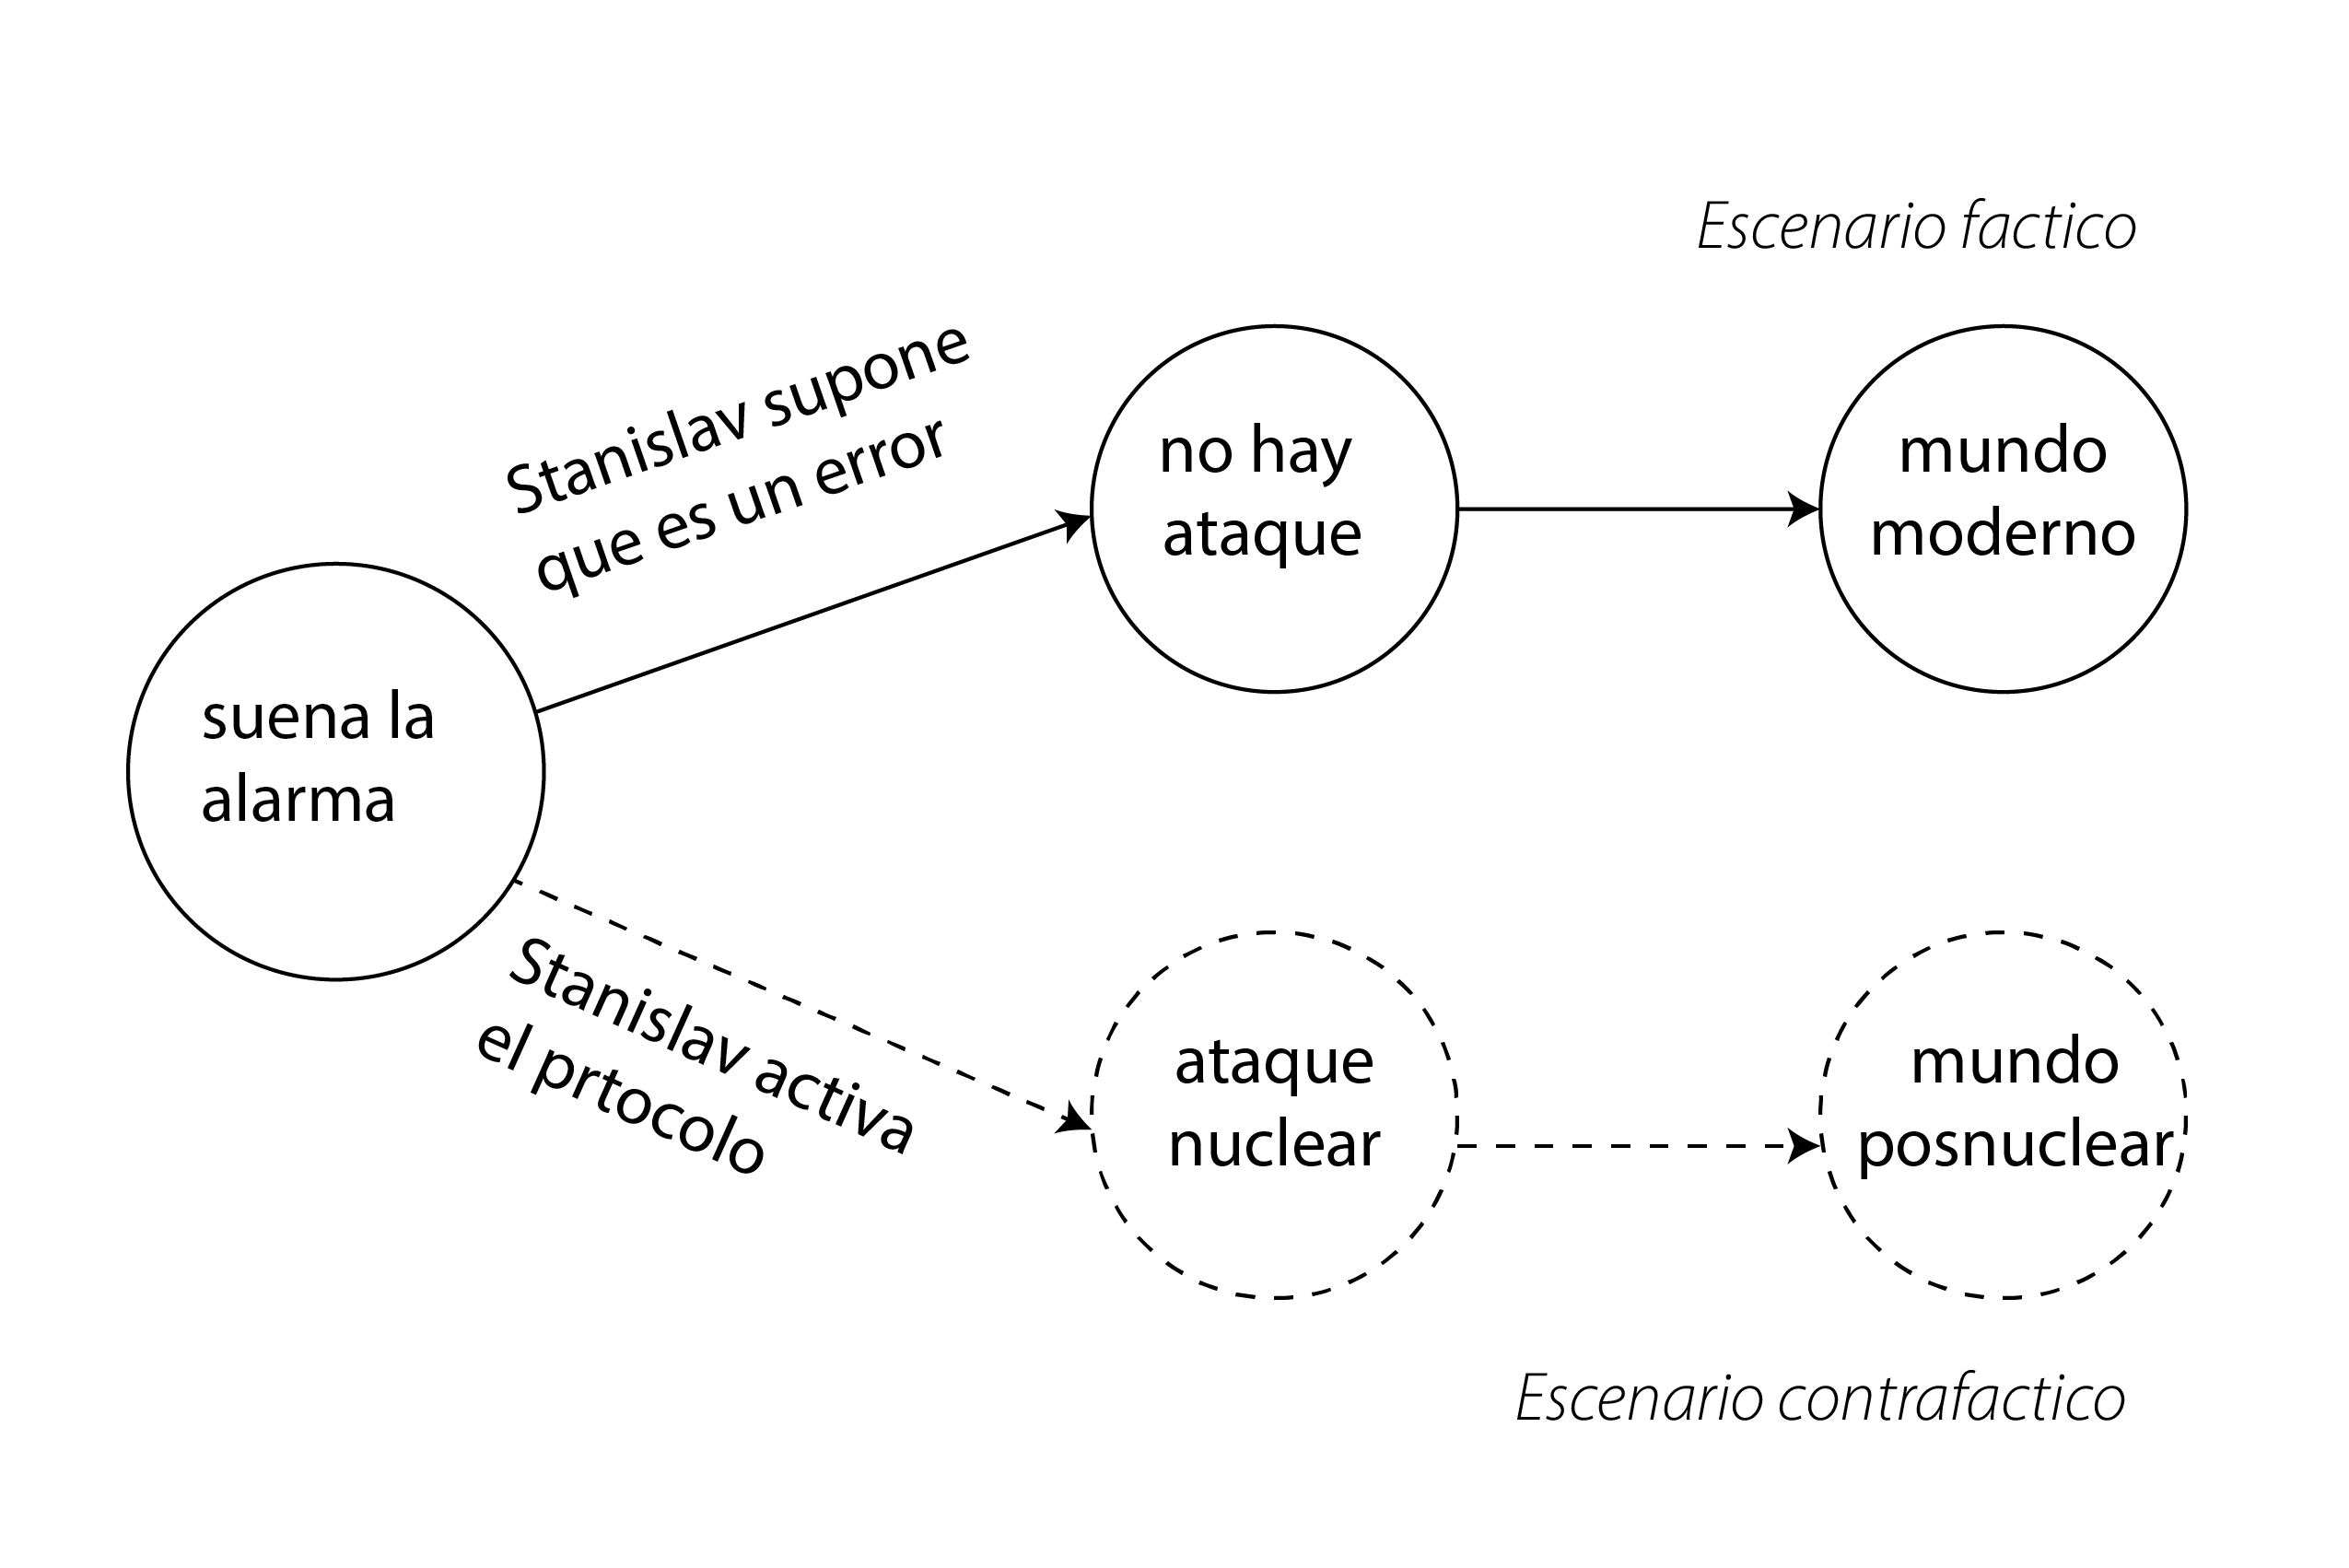
\includegraphics{./imgs/fig-01.png}

}

\end{figure}

\begin{tcolorbox}[enhanced jigsaw, breakable, rightrule=.15mm, colbacktitle=quarto-callout-tip-color!10!white, bottomtitle=1mm, arc=.35mm, titlerule=0mm, left=2mm, toprule=.15mm, leftrule=.75mm, colback=white, opacitybacktitle=0.6, opacityback=0, colframe=quarto-callout-tip-color-frame, bottomrule=.15mm, coltitle=black, toptitle=1mm, title=\textcolor{quarto-callout-tip-color}{\faLightbulb}\hspace{0.5em}{De qué hablamos cuando hablamos de contrafactuales}]
Utilizando el marco conceptual de los \emph{potential outcomes} de
Rubin(Rubin
1974)\marginpar{\begin{footnotesize}\leavevmode\vadjust pre{\protect\hypertarget{ref-rubin1974estimating}{}}%
Rubin, Donald B. 1974. {«Estimating causal effects of treatments in
randomized and nonrandomized studies.»} \emph{Journal of educational
Psychology} 66 (5): 688.\vspace{2mm}\par\end{footnotesize}},
un contrafactual es el resultado que hubiera ocurrido para una unidad
experimental (por ejemplo, una persona, un paciente, un animal de
laboratorio o un país) si hubiera recibido un tratamiento diferente del
que realmente recibió. Este concepto es fundamental para entender los
efectos causales. Nos permite definir lo que entendemos por causa: la
diferencia entre lo que realmente sucedió y lo que hubiera sucedido en
un escenario alternativo.

En pocas palabras:

\begin{itemize}
\item
  \textbf{para alguien que recibió el tratamiento, el contrafactual es
  lo que habría sucedido si no hubiera recibido el tratamiento}. Por
  ejemplo, si un paciente recibió un nuevo medicamento y se recuperó, el
  resultado contrafactual es su estado de salud si no hubiera recibido
  el medicamento. Esto nos ayuda a aislar el efecto del medicamento;
\item
  \textbf{para alguien que no recibió el tratamiento, el contrafactual
  es lo que hubiera sucedido si hubiera recibido el tratamiento}. Por
  ejemplo, si un estudiante no asistió a un programa de tutoría y
  reprobó un examen, el contrafactual es su calificación hipotética si
  hubiera asistido al programa.
\end{itemize}

Dado que cada unidad recibe solo un tratamiento, solo podemos observar
un resultado: el resultado real. El resultado contrafactual es, por
definición, \textbf{inobservable}. Esto se conoce a menudo como el
\textbf{problema fundamental de la inferencia causal}. Debido a que no
podemos observar simultáneamente ambos resultados potenciales para el
mismo individuo, vamos a usar métodos y suposiciones estadísticas para
estimar los efectos promedio del tratamiento en grupos de individuos.
Más de esto en los próximos capítulos.
\end{tcolorbox}

¿Para qué sirve, entonces, construir contrafácticos, imaginar cosas que
no ocurrieron y que nunca ocurrirán? Veamos otra historia.

Este cuadro que se ve a continuación se llama \emph{Praying Hands} y fue
pintado por Albrecht Durero. Es una de las obras más importantes de su
siglo.

\begin{figure}

{\centering 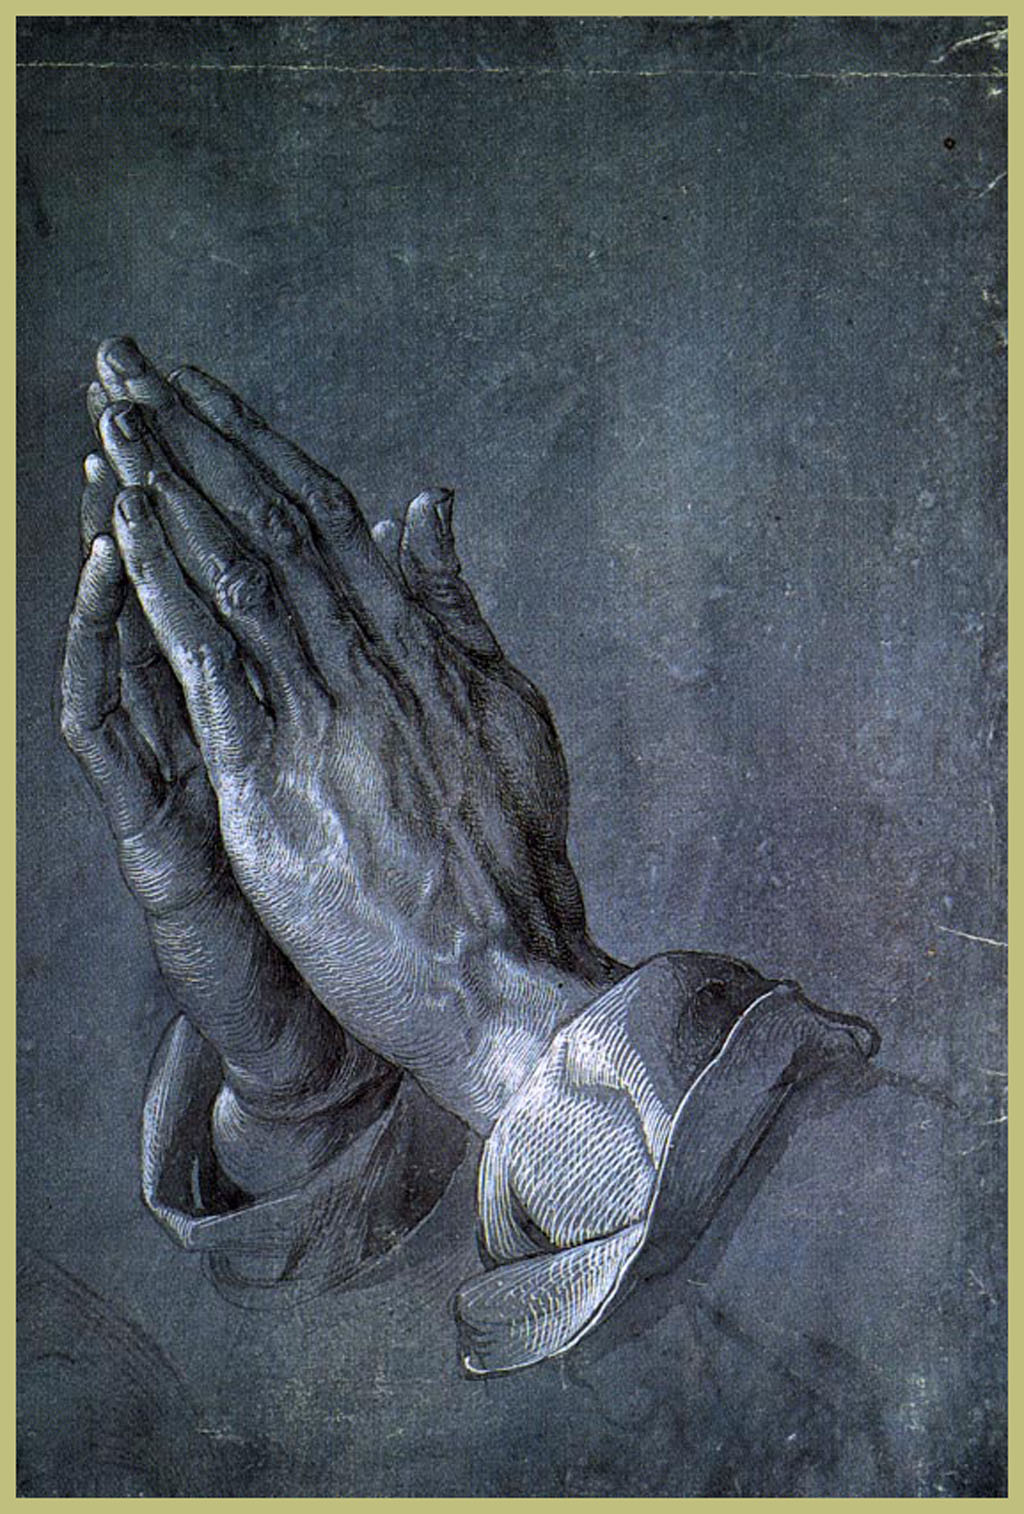
\includegraphics[width=3.125in,height=\textheight]{./imgs/Study-of-Praying-Hands-Durer-Albrecht-1508-2.jpg}

}

\caption{\emph{Praying Hands} de Albrecht Durero.}

\end{figure}

Los Durero eran una familia de mineros pobres del sur de Alemania. Dos
de sus hijos, Albrecht y Joseph, tenían talento para el dibujo y
decidieron hacer un pacto: uno estudiaría en Núremberg durante cuatro
años mientras el otro trabajaría en las minas para pagar su educación.
Decidirían quién haría qué cosa lanzando una moneda al aire. Pasado ese
tiempo, intercambiarían lugares.

El azar favoreció a Albrecht. Durante esos cuatro años, se convirtió en
un pintor famoso y regresó a casa para cumplir su parte del acuerdo. Sin
embargo, al llegar, Joseph lo recibió con una triste noticia: era
demasiado tarde. El arduo trabajo en la mina le había provocado una
artritis severa, lo que le impedía sostener un pincel. Como único
tributo a su sacrificio, Albrecht decidió pintar sus manos.

Ahora tenemos dos escenarios contrafácticos: lo que le hubiera sucedido
a Albretch si se quedaba en la mina y lo que le hubiera sucedido a
Joseph si se iba a estudiar a Núremberg. De modo que el escenario sería
así:

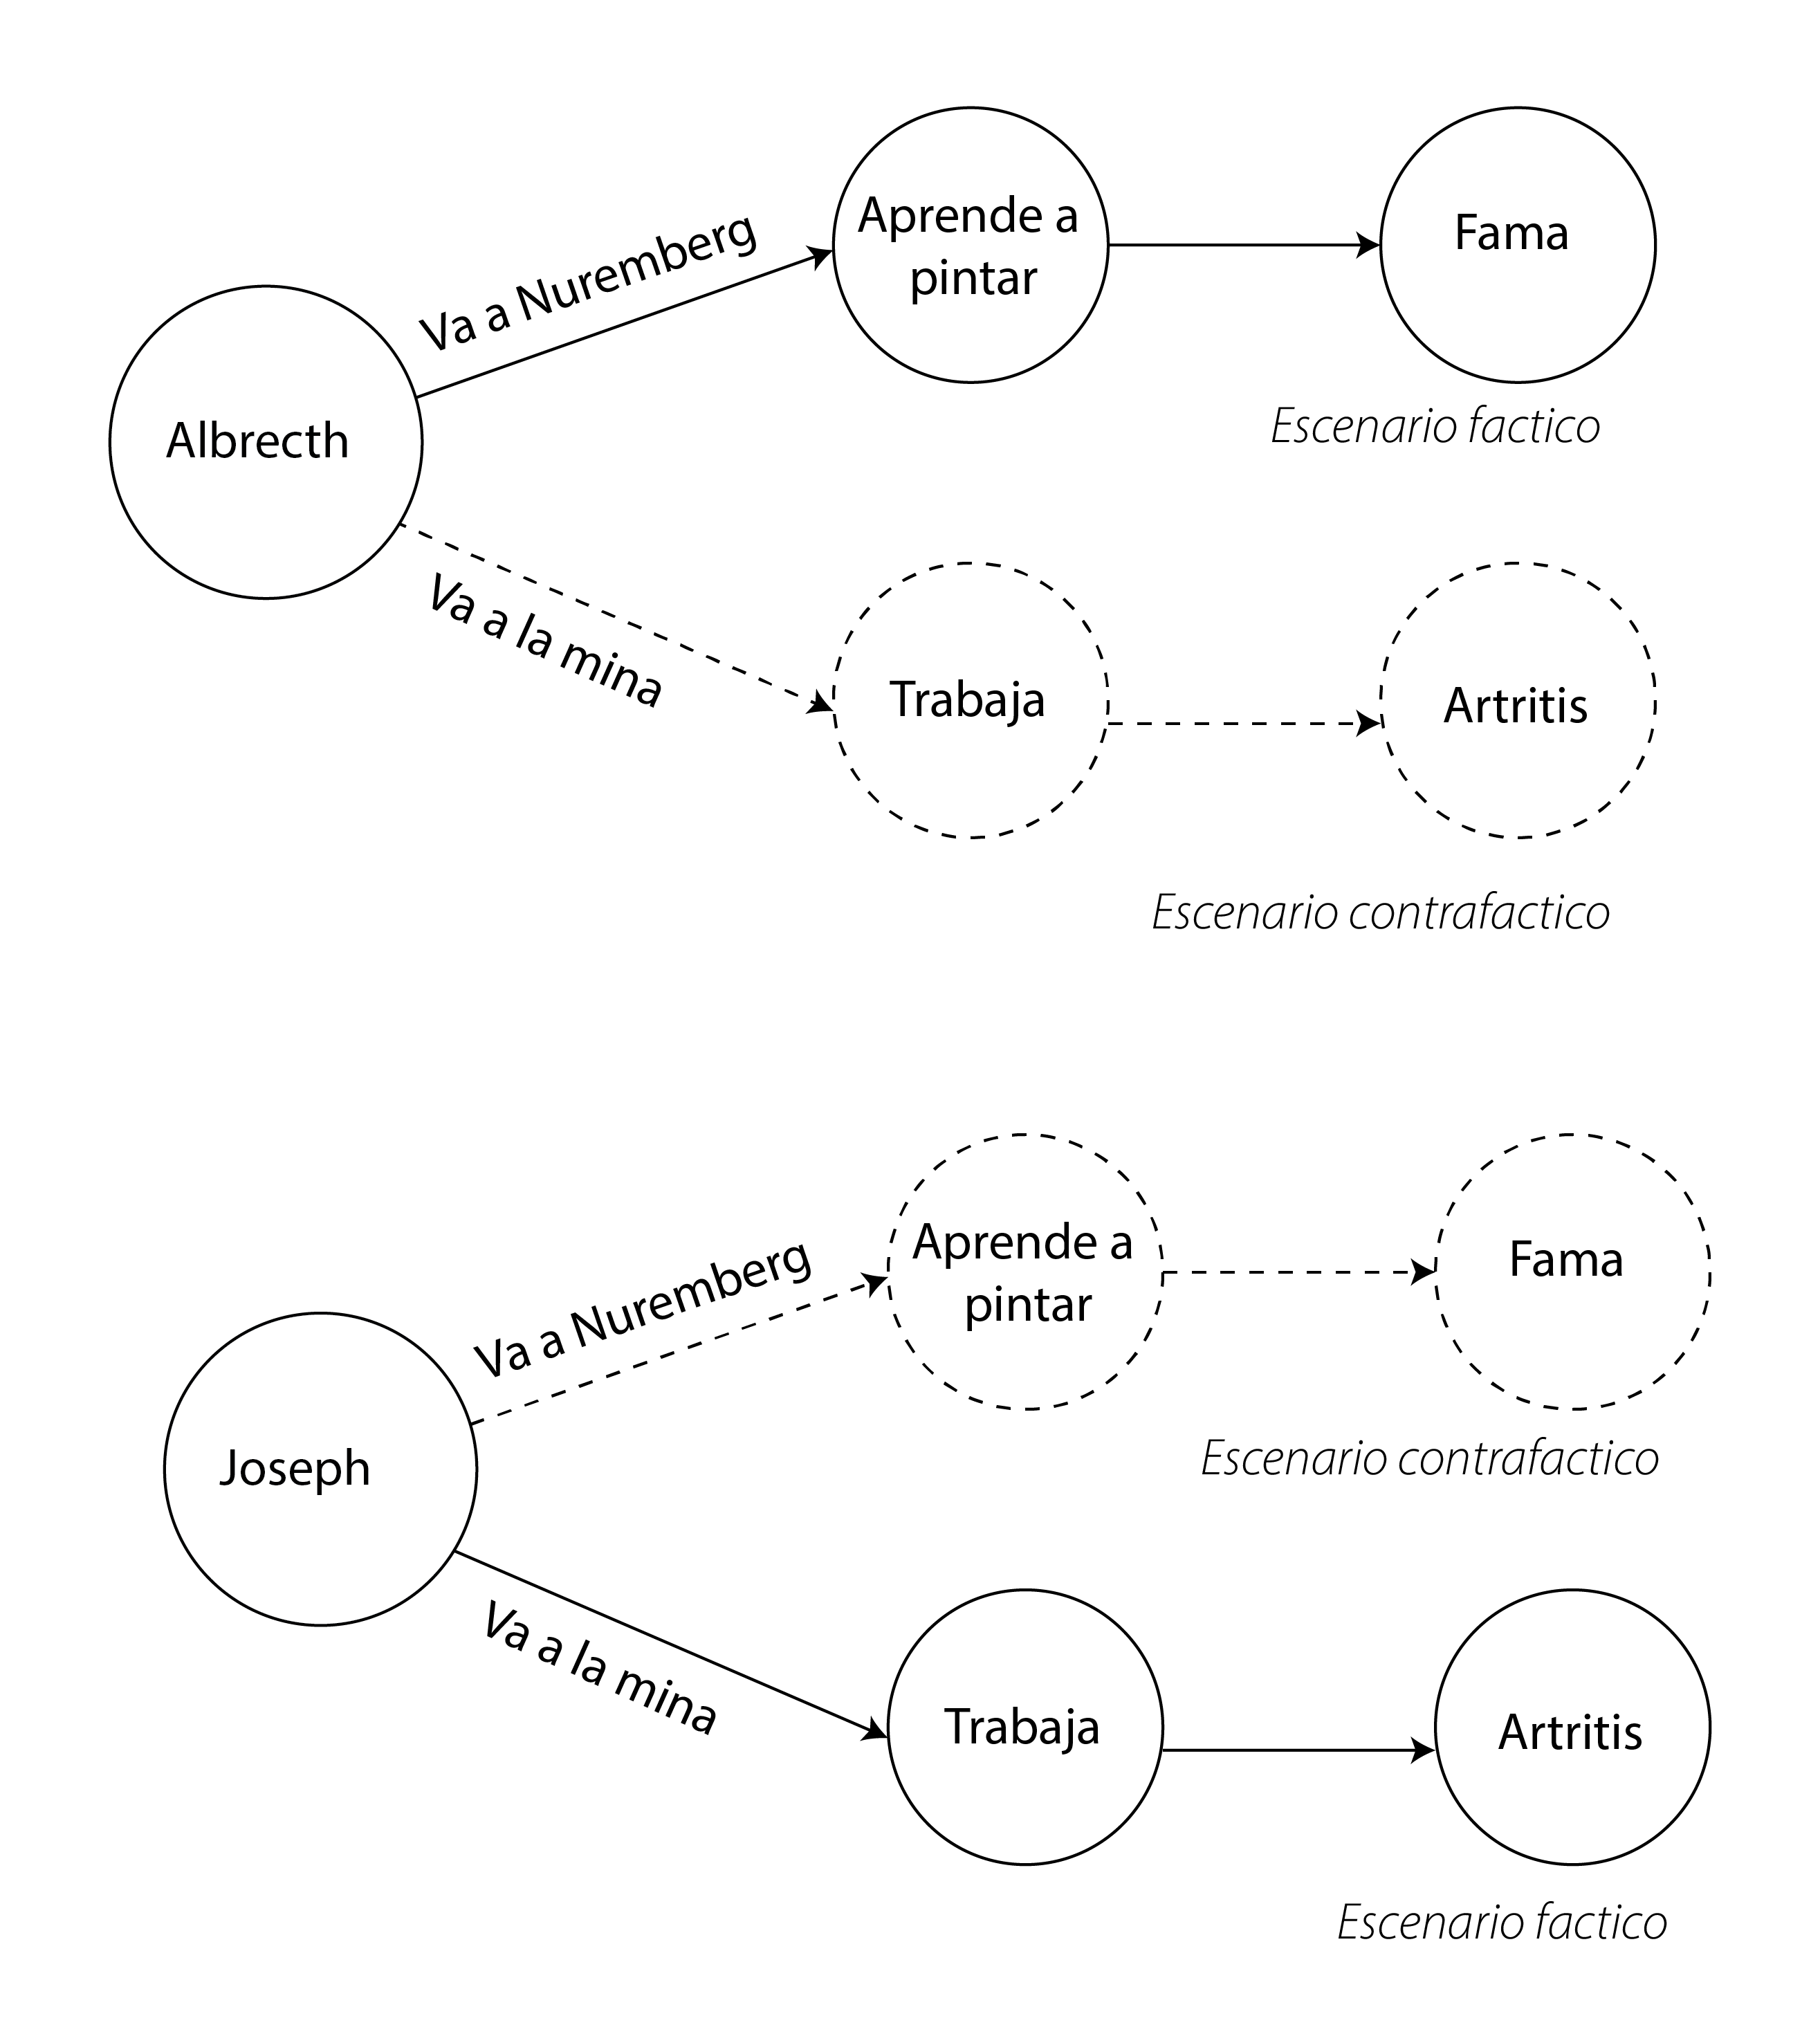
\includegraphics{./imgs/fig-02.png}

Ambos son hermanos, y uno podría creer que, entre otra cosas, comparten
cierto talento y sensibilidad artística. Asimismo, uno podría suponer
que el destino de Joseph serviría para suponer con mayor precisión lo
que ``le hubiera pasado a Albretch de no ir a Núremberg'' (escenario
contrafactico). De forma inversa, el destino de Albretch representaría
``lo que le hubiera pasado a Joseph si hubiera podido ir a Núremberg''
(escenario contrafáctico). Entonces imaginar escenarios contrafácticos
nos permiten estimar el efecto de ir a Núremberg o de quedarse.

Ahora bien, ¿es Joseph lo mismo que Albrecth? Si la moneda hubiera
favorecido a Joseph, ¿habría un Durero pintor famoso? Bueno, no estamos
seguros de eso. Sobre lo que si podemos estar seguros es que -pese a
parecidos- ellos no son exactamente la misma persona y quizás había
diferencias en talentos o en suceptibilidad a la artritis lo que hace
que el destino de uno funcione como un símil o proxy de su destino
contrafáctico pero no el destino en sí mismo. Con estas ideas podemos
armar un marco teóprico donde esos efectos se puedan estimar.

Supongamos que quiero evaluar la efectividad de la aspirina para mitigar
el dolor de cabeza. Me duele la cabeza y lo que quiero es saber el
efecto diferencial entre tomar y no tomar esa aspirina. Es decir, en el
tiempo 0 estoy con dolor de cabeza y en el tiempo 1 debería haber dos
versiones mías (como si una no fuera suficiente): la que tomó la
aspirina y la que no. A cada una de ellas les tendría que preguntar
cuánto les duele la cabeza (esto es el \emph{outcome} de mi
comparación). No hace falta ser demasiado astuto para darse cuenta que
esto es imposible ya que solo nos será posible observar una de esas
versiones, mientras que la otra será un contrafáctico.

De esto vamos a hablar en este capítulo, utilizando como marco teórico a
los \emph{potential outcomes}. Estas ideas terminan de tomar forma en la
versión que conocemos en las ciencias sociales propuestas por
Rubin(Rubin
1974)\marginpar{\begin{footnotesize}\leavevmode\vadjust pre{\protect\hypertarget{ref-rubin1974estimating}{}}%
Rubin, Donald B. 1974. {«Estimating causal effects of treatments in
randomized and nonrandomized studies.»} \emph{Journal of educational
Psychology} 66 (5): 688.\vspace{2mm}\par\end{footnotesize}}.

\hypertarget{potential-outcomes}{%
\section{\texorpdfstring{\emph{Potential
outcomes}}{Potential outcomes}}\label{potential-outcomes}}

Lo que nos proponen los \emph{potential outcomes} es la definición del
efecto causal como la comparación de dos estados del mundo. En una
versión del mundo, la ``actual'' (u obsevada), me tomo una aspirina y a
las dos horas registro la severidad de mi dolor de cabeza. En cambio, en
la otra versión del mundo, la ``contrafactual'', no me tomo la aspirina
y a las dos horas registro la severidad del dolor. A partir de esto, la
tradición de los \emph{potential outcomes} define al efecto causal de
tomar una aspirina en el dolor de cabeza como la diferencia entre esas
dos mediciones.

Todo muy lindo, pero como ya estarán sospechando es imposible calcular
un efecto que está expresado en función de un contrafactual, ya que no
lo podemos observar. Pero no se preocupen que le vamos a encontrar la
vuelta.

Empecemos con un poco de notación que nos va a ayudar a acomodar las
ideas. Por simplicidad, vamos a asumir una variable binaria para la
asignación del grupo experimental (por ejemplo, tratamiento y control).
Esta variable vale \(1\) si la unidad \emph{i} recibe el tratamiento y
\(0\) si no, o sea, si pertenece al grupo control. Cada unidad \(i\) va
a tener dos \emph{potential outcomes}: \(Y_i^1\) si la unidad recibió el
tratamiento y \(Y_i^0\) si no. Esto significa que una unidad
experimental en el mismo momento del tiempo va a recibir y no recibir el
tratamiento, o sea, alguno de estos va a ser contrafactual\sidenote{\footnotesize De
  ahí el nombre de \emph{potential}, porque se trata de posibles estados
  del mundo. Un estado en el que la unidad \(i\) recibe el tratamiento y
  uno en el que no.}.

Los \emph{outcomes} observables difieren de los potenciales. Los
potenciales son variables aleatorias parcialmente latentes --- solo uno
de sus valores se revela por unidad ---, mientras que los observables
son sus realizaciones medibles. Hay una ecuación que nos permite definir
el \emph{outcome} observable (\(Y^i\)) en función de los potenciales, se
llama la \emph{switching equation}:

\begin{equation}\protect\hypertarget{eq-switching}{}{
Y_i = D_i Y_i^1 + (1-D_i) Y_i^0 
}\label{eq-switching}\end{equation}

Donde \(D_i\) vale \(1\) si la unidad \emph{i} recibió el tratamiento
(entonces \(Y_i=Y_i^1\)) y \(0\) si no (entonces \(Y_i=Y_i^0\)). Vale la
pena notar que \(Y_i\), el \emph{outcome} observable, no tiene ningún
supraíndice ya que no es más potencial. Esto también es una forma de
hacer explícito el problema del \emph{outcome observable} porque,
dependiendo el valor que adopte \(D_i\) uno de los términos se vuelve
cero. Si \(D_i=0 \rightarrow Y_i=Y_i^0\) ya que el término \(D_i Y_i^1\)
vale 0. Si por el contrario \(D_i=1 \rightarrow Y_i=Y_i^1\) porque el
término \((1-D_i) Y_i^0\) vale cero. Esta es una forma sofisticada de
decir que el outcome observable sólo es posible en una de las dos formas
de \(D_i\).

Usando esta notación definimos el efecto causal del tratamiento para una
unidad \(i\) como:

\begin{equation}\protect\hypertarget{eq-deltai}{}{
\delta_i = Y_i^1 - Y_i^0 
}\label{eq-deltai}\end{equation}

Donde queda claro que para estimar el efecto causal de acuerdo a la
tradición de los \emph{potential outcomes} debemos conocer dos estados
del mundo a los que es imposible acceder simultáneamente. Y aquí yace el
\textbf{problema fundamental de la inferencia causal}: para calcular el
efecto causal se requiere acceso a datos que siempre nos van a faltar:
los contrafácticos(Rubin
1974)\marginpar{\begin{footnotesize}\leavevmode\vadjust pre{\protect\hypertarget{ref-rubin1974estimating}{}}%
Rubin, Donald B. 1974. {«Estimating causal effects of treatments in
randomized and nonrandomized studies.»} \emph{Journal of educational
Psychology} 66 (5): 688.\vspace{2mm}\par\end{footnotesize}}.

\hypertarget{efecto-promedio-del-tratamiento}{%
\section{Efecto promedio del
tratamiento}\label{efecto-promedio-del-tratamiento}}

Al igual que los \emph{potential outcomes}, el efecto para la unidad
\(i\) (\(\delta_i\)) también es una variable aleatoria, y su esperanza
es lo que vamos a llamar el efecto promedio del tratamiento
(\textbf{ATE}\sidenote{\footnotesize Del inglés \emph{Average treatment effect}.}). El
\textbf{ATE} va a ser la magnitud de interés en nuestros experimentos,
el efecto promedio de mi tratamiento. Este se define de la siguiente
forma:

\begin{equation}\protect\hypertarget{eq-ATE}{}{
\begin{array}
_ATE &=& E[\delta_i] \\
&=& E[Y_i^1 - Y_i^0] \\
&=& E[Y_i^1] - E[Y_i^0] 
\end{array}
}\label{eq-ATE}\end{equation}

Ahora vamos a definir el efecto promedio, pero para el grupo tratado (es
decir, los participantes asignados al grupo tratamiento, con \(D_i=1\)):

\begin{equation}\protect\hypertarget{eq-ATT}{}{
\begin{array}
_ATT &=& E[\delta_i|D_i=1] \\
&=& E[Y_i^1 - Y_i^0|D_i=1] \\
&=& E[Y_i^1|D_i=1] - E[Y_i^0|D_i=1] 
\end{array}
}\label{eq-ATT}\end{equation}

Esta magnitud se llama \textbf{ATT}\sidenote{\footnotesize Del inglés \emph{Average
  treatment effect for the treated}.} y se calcula de la misma forma que
el \textbf{ATE}, pero condicionando los \(\delta_i\) al valor de \(D_i\)
igual a 1. De manera análoga, definimos el efecto promedio pero para el
grupo no tratado\sidenote{\footnotesize Del inglés \emph{Average treatment effect for
  the untreated}.}(\(D_i=0\))

\begin{equation}\protect\hypertarget{eq-ATU}{}{
\begin{array}
_ATU &=& E[\delta_i|D_i=0] \\
&=& E[Y_i^1 - Y_i^0|D_i=0] \\
&=& E[Y_i^1|D_i=0] - E[Y_i^0|D_i=0] 
\end{array}
}\label{eq-ATU}\end{equation}

Ojo con confundir estos tres conceptos. Creo que el \textbf{ATE} es
autoexplicativo, pero se suele confundir \textbf{ATT} y \textbf{ATU}. En
el primer caso, el \textbf{ATT} es, como su nombre lo indica, el
\emph{efecto promedio del tratamiento para el grupo de tratamiento}.
Estamos calculando la esperanza de los \(\delta_i\) de los individuos
pertenecientes al grupo tratamiento. Esto involucra tanto sus \(Y^1_i\)
como sus \(Y^0_i\). En el segundo caso, el \textbf{ATU} es el
\emph{efecto promedio del tratamiento para el grupo de no tratamiento},
es decir, la esperanza de los \(\delta_i\) para los individuos
pertenecientes al grupo control.

Es un error común confundir estos efectos promedios con magnitudes no
potenciales pero, como se observa de sus fórmulas, tanto estos últimos
dos como \textbf{el ATE no se pueden calcular en la práctica}.

En las secciones siguientes vamos a ver como, cumpliendo ciertas
condiciones\sidenote{\footnotesize \emph{Spoiler}: Asignación aleatoria de las
  unidades experimentales a los grupos.}, podemos estimar el
\textbf{ATE} a partir de los \emph{outcomes} observables.

\hypertarget{diferencia-de-medias-simple}{%
\section{Diferencia de medias
simple}\label{diferencia-de-medias-simple}}

¿Qué es lo que sí podemos observar? Una magnitud que, a priori,
podríamos creer que va a estar relacionada con el \textbf{ATE}: la
diferencia de medias entre los \emph{outcomes} observados del grupo
tratamiento y el grupo control. La vamos a llamar
\textbf{SDO}\sidenote{\footnotesize Del inglés \emph{simple difference in outcomes}.}
y se calcula de la siguiente forma:

\begin{equation}\protect\hypertarget{eq-SDO}{}{
\begin{array}
_SDO &=& E[Y_i^1|D_i=1] - E[Y_i^0|D_i=0] \\
&=& \frac{1}{N_T} \sum_{i=1}^{N_T} (y_i|d_i=1) - \frac{1}{N_C} \sum_{i=1}^{N_C} (y_i|d_i=0)
\end{array}
}\label{eq-SDO}\end{equation}

Donde \(N_T\) y \(N_C\) son la cantidad de individuos en el grupo
tratamiento y control respectivamente (y \(N_T + N_C = n\)). Todo muy
lindo, pero operemos un poquito para ver hasta que punto el \textbf{SDO}
es un estimador insesgado del \textbf{ATE}. Empecemos escribiendo el
\textbf{ATE} como una suma pesada del \textbf{ATT} y el \textbf{ATU}:

\begin{equation}\protect\hypertarget{eq-sesgos}{}{
\begin{array}
_ATE &=& \pi ATT + (1-\pi) ATU \\
&=& \pi E[Y_i^1|D_i=1] - \pi E[Y_i^0|D_i=1] + \\
& & (1-\pi) E[Y_i^1|D_i=0] - (1-\pi) E[Y_i^0|D_i=0] \\
&=& \bigl\{ \pi E[Y_i^1|D_i=1] + (1-\pi) E[Y_i^1|D_i=0] \bigl\} - \\
& & \bigl\{ \pi E[Y_i^0|D_i=1] + (1-\pi) E[Y_i^0|D_i=0] \bigl\}
\end{array}
}\label{eq-sesgos}\end{equation}

Con \(\pi = N_T/n\) y \(1 - \pi = N_C/n\). Es decir \(\pi\) es la
proporción de individuos tratados y \(1 - \pi\) es la proporción de
individuos no tratados.

Operando con la Ecuación~\ref{eq-sesgos} podemos despejar la diferencia
entre los \emph{outcomes} observables (\textbf{SDO}) y ver cómo esta se
relaciona con el resto de las magnitudes definidas\sidenote{\footnotesize Pueden ver
  el despeje numérico en detalle en el capítulo 4 de (Cunningham
  2021).\linebreak\linebreak\leavevmode\vadjust pre{\protect\hypertarget{ref-cunningham2021causal}{}}%
Cunningham, Scott. 2021. \emph{Causal inference: The mixtape}. Yale
university press.\linebreak}.

\[
\begin{array}
_E[Y_i^1|D_i=1] - E[Y_i^0|D_i=0] &=& ATE \\
&+& ( E[Y_i^0|D_i=1] - E[Y_i^0|D_i=0] ) \\
&+& (1-\pi) (ATT - ATU)
\end{array}
\]

Que podemos reescribir como:

\begin{equation}\protect\hypertarget{eq-SDOdecomp}{}{
\begin{array}
_\underbrace{\frac{1}{N_T} \sum_{i=1}^{N_T} (y_i|d_i=1) - \frac{1}{N_C} \sum_{i=1}^{N_C} (y_i|d_i=0)}_\text{Diferencia de los outcomes} &=& \underbrace{ATE}_\text{Efecto promedio del tratamiento} \\
&+& \underbrace{( E[Y_i^0|D_i=1] - E[Y_i^0|D_i=0] )}_\text{Sesgo de selección} \\
&+& \underbrace{(1-\pi) (ATT - ATU)}_\text{Sesgo de efecto heterogéneo}
\end{array}
}\label{eq-SDOdecomp}\end{equation}

Lo que puede verse en la Ecuación~\ref{eq-SDOdecomp} es que si
pudiéramos asegurar de alguna forma que los sesgos de selección y de
efecto heterogéneo fueran cero, el \textbf{SDO} sería un buen estimador
del \textbf{ATE} que es, al fin y al cabo, el efecto causal promedio que
nos interesa en nuestro experimento.

O sea que la clave del diseño experimental va a ser encontrar la forma
de asegurar que esos sesgos sean nulos. Veamos mejor que representan
para poder entender cómo minimizarlos.

\hypertarget{sesgo-de-selecciuxf3n}{%
\subsection{Sesgo de selección}\label{sesgo-de-selecciuxf3n}}

Miremos con detenimiento la fórmula a la que llamamos sesgo de selección
\(E[Y_i^0|D_i=1] - E[Y_i^0|D_i=0]\). Si la definimos a partir de esta
ecuación representa la diferencia entre los dos grupos si nunca hubiese
habido un tratamiento en primer lugar. Es decir, son las diferencias
inherentes entre los dos grupos. Estas diferencias aparecen al
\textbf{seleccionar} individuos en un grupo y no en el otro, por eso lo
llamamos sesgo de selección. Por el contrario, mientras más se parezcan
en el outcome \(Y_i^0\) los individuos asignados a uno u otro grupo
\(D\), más cercano a cero será el sesgo de selección. Entonces, sería
ideal medir el sesgo de selección ya que es una medida de cuán lejos
está el estimador del \textbf{ATE} (el \textbf{SDO}) del verdadero
valor. Sin embargo, el primer término de la ecuación es un
contrafáctico. No nos queda otra alternativa que buscar una condición en
donde, aunque no podamos medirlo, podamos confiar en que el sesgo de
selección tiene esperanza igual a cero.

\hypertarget{sesgo-de-tratamiento-heteroguxe9neo}{%
\subsection{Sesgo de tratamiento
heterogéneo}\label{sesgo-de-tratamiento-heteroguxe9neo}}

Esta tercera componente, \((1-\pi) (ATT - ATU)\), es un poco más difícil
de explicar. Así definido se puede decir que es la diferencia entre el
efecto promedio del tratamiento para el grupo tratamiento (el
\textbf{ATT}) y la misma para el grupo control (el \textbf{ATU})
multiplicada por la proporción de sujetos que está en el grupo control.
A diferencia del sesgo de selección, en este caso no se trata de una
diferencia entre los dos grupos si no hubiera habido tratamiento, sino
que es la diferencia entre el efecto del tratamiento para el grupo
tratado y el efecto del tratamiento para el grupo control. En otras
palabras, este sesgo cuantifica las diferencias en \emph{sensibilidad}
al tratamiento por cada uno de los grupo. Por ejemplo, si estamos
testeando una droga para mejorar la resistencia aeróbica y en nuestro
grupo tratamiento tenemos a 90\% de asmáticos/as mientras que en el
grupo control sólo a un 10\%, es esperable que los efectos del
tratamiento en cada uno de estos grupos sean distintos. Pero ojo,
recordamos que ni el \textbf{ATT} y el \textbf{ATU} pueden ser medidos
porque incluyen contrafácticos en su definición.

Ahora que entendemos qué representa cada sesgo, podemos buscar una
condición en donde la esperanza de ambos sesgos sea igual a 0 para que,
de esta forma, el SDO sea finalmente un estimador insesgado del ATE. Esa
condición es la independencia.

\hypertarget{independencia}{%
\section{Independencia}\label{independencia}}

La definición de independencia en el contexto de los \emph{potential
outcomes}, es la siguiente:

\[
(Y^0, Y^1) \perp D
\]

Momento cerebrito, pensemos una poco qué quiere decir. Esto significa
que la asignación de los participantes al grupo control o tratamiento
(\(D\)) no depende de los \emph{outcomes} potenciales de ese individuo
\sidenote{\footnotesize El símbolo de perpendicularidad quiere simbolizar eso, que no
  hay relación entre los \emph{outcomes} potenciales y la asignación a
  los grupos.}.

Vamos a pensarlo con un ejemplo concreto. Imaginen que tenemos un grupo
de participantes para poner a prueba una cirugía experimental como
alternativa a un tratamiento médico no quirúrgico, que es el tratamiento
establecido. Si la asingación de individuos a uno u otro grupo la hace
un médico según su criterio -por ejemplo, no asignando a pacientes de
edad avanzada al grupo tratamiento por el riesgo asociado a una cirugía,
o asignando a pacientes cuyo pronóstico con el método tradicional vea
poco favorable al grupo control- entonces la asignación depende de los
posibles resultados y, por lo tanto, no hay independencia. Si en cambio
tiráramos una moneda antes de recibir a cada paciente, podríamos
asegurar la independencia.

La independencia implica que se cumpla:

\begin{equation}\protect\hypertarget{eq-independencia}{}{
\begin{array}
_E[Y^1|D=1] - E[Y^1|D=0] &=& 0 \\
E[Y^0|D=1] - E[Y^0|D=0] &=& 0
\end{array}
}\label{eq-independencia}\end{equation}

Es decir, que la esperanza de los \emph{outcomes} para los participantes
que fueron asignados tanto al grupo tratamiento y al grupo control
serían iguales si pudiéramos medir a ambos en \emph{mundo tratamiento} o
en \emph{mundao control}\sidenote{\footnotesize Tengamos en cuenta que tanto
  \(E[Y^1|D=0]\) como \(E[Y^0|D=1]\) son escenarios contrafácticos.}.
Ojo que esto no implica que la esperanza del \emph{outcome} para
tratamiento en los tratados sea igual a la esperanza de no tratamiento
en los controles (\(E[Y^1|D=1] - E[Y^0|D=0] = 0\)), ni igual a la
esperanza de no tratamiento de los tratados
(\(E[Y^1|D=1] - E[Y^0|D=1] = 0\)).

¿Qué implicancias tiene las igualdades presentadas en
Ecuación~\ref{eq-independencia} en los sesgos que vimos en la ecuación
Ecuación~\ref{eq-sesgos}? Empecemos por el sesgo de selección
(\(E[Y^0|D=1] + E[Y^0|D=0]\)). Vemos que, de acuerdo a la primera línea
de Ecuación~\ref{eq-independencia}, de ser independiente la asignación
del grupo experimental, este sesgo sería cero. Pensemos un poco. La
condición de independencia nos dice que, si ninguno de los dos grupos
fueran no tratados, ambos tendrían el mismo \emph{outcome}, lo que
sugiere que es razonable considerar nulo el sesgo de selección.

La relación del sesgo de efecto heterogéneo (\((1-\pi) (ATT - ATU)\))
con la independencia es un poquito más difícil de demostrar. Olvidémonos
del \((1-\pi)\) por un momento. Reescribamos los efectos \textbf{ATT} y
\textbf{ATU}:

\[
\begin{array}
_ATT &=& E[Y^1|D=1] - E[Y^0|D=1] \\
ATU &=& E[Y^1|D=0] - E[Y^0|D=0] 
\end{array}
\]

Y ahora restemos ambos términos:

\begin{equation}\protect\hypertarget{eq-sesgohet}{}{
\begin{array}
_ATT - ATU &=& E[Y^1|D=1] - E[Y^0|D=1] - ( E[Y^1|D=0] - E[Y^0|D=0] )\\
&=& \bigl\{ E[Y^1|D=1] - E[Y^1|D=0] \bigl\} + \bigl\{ E[Y^0|D=0] - E[Y^0|D=1] \bigl\} 
\end{array}
}\label{eq-sesgohet}\end{equation}

Reescrito de esta forma podemos ver que los dos primero términos de
Ecuación~\ref{eq-sesgohet} se hacen cero por la primera línea de la
Ecuación~\ref{eq-independencia}, y los últimos dos se hacen cero por la
segunda.

Finalmente, demostramos que si hay independencia en la asignación de los
grupos, la diferencia de las medias simple (\textbf{SDO}) entre el grupo
tratado y el grupo control es un estimador insesgado del \textbf{ATE}.

\hypertarget{sutva}{%
\section{SUTVA}\label{sutva}}

En este capítulo hemos presentado un marco teórico para definir un
efecto causal. A ese efecto causal lo llamamos \textbf{ATE} y vimos que
es imposible calcularlo por la existencia de contrafácticos, pero que
puede ser estimado por una medida observable: la \textbf{SDO}. También
vimos que \textbf{SDO} contiene al \textbf{ATE} y a un par de sesgos.
Estos sesgos deberían hacerse cero si el supuesto de independencia se
cumple.

¿Podría pasar que un efecto causal no pueda ser estimado con este marco
teórico? Sí, hay un límite en este marco en donde todas estos cáclulos
(medibles o no) no son posibles. Si vamos al corazón mismo de todos
estos cálculos la condición que debe cumplirse para que todo sea posible
es que las \(Y_i\) sean \emph{restables} (o, dicho de otra forma, que
representen lo mismo). A este supuesto se lo llama \textbf{SUTVA} que es
la abreviatura de \textbf{stable unit treatment value assumption}. Vamos
a reformularlo. \textbf{SUTVA} implica que cada unidad \(i\) recibe la
misma dosis de tratamiento.

El \textbf{SUTVA} se cumple, la respuesta de un individuo expuesto a
tratamiento será la misma: \emph{1)} sin importar cómo el participante
fue asignado al tratamiento, y \emph{2)} sin importar los tratamientos
recibidos por las otras unidades.

Sin embargo, en la práctica estos supuestos pueden fallar. En
particular, la segunda condición ---la ausencia de interferencia entre
unidades--- puede violarse por fenómenos sociales, conductuales o
institucionales que modifican la respuesta de los individuos en función
de lo que ocurre con otros. Algunos ejemplos clásicos de estas
violaciones son la rivalidad compensatoria, la desmoralización
resentida, la difusión o imitación de tratamientos y la ecualización
compensatoria de tratamientos.

La rivalidad compensatoria ocurre cuando los individuos del grupo
control, al saber (o sospechar) que no están recibiendo el tratamiento,
reaccionan esforzándose más para ``compensar'' esa desventaja. Por
ejemplo, en un estudio educativo, los estudiantes que no reciben una
nueva intervención pedagógica podrían estudiar más por su cuenta para no
quedar atrás. Esto genera que sus resultados mejoren artificialmente, lo
que reduce la diferencia observada entre tratamiento y control y, por lo
tanto, subestima el efecto causal real. En notación de \emph{potential
outcomes}, esto se traduce en que el resultado observable
(\(Y_i^0|D_i=0\)) tiene agregado un efecto ``compensatorio'' que lo hace
más grande que su contrafáctico (\(Y_i^0|D_i=1\)), o sea, la respuesta
al no-tratamiento en el grupo tratamiento.

En contraste, la desmoralización resentida aparece cuando los individuos
del grupo control, al percibirse en desventaja, se desmotivan o reducen
su esfuerzo. Siguiendo el mismo ejemplo, estudiantes que no reciben la
intervención podrían perder interés o sentirse injustamente tratados,
empeorando su desempeño. En este caso, la diferencia entre los grupos se
amplifica, lo que puede llevar a sobreestimar el efecto del tratamiento.

La difusión o imitación de tratamientos (también conocida como
\emph{spillover}) ocurre cuando el tratamiento asignado al grupo tratado
se filtra hacia el grupo control. Esto puede suceder, por ejemplo, si
los participantes comparten información, prácticas o recursos. Como
resultado, algunos individuos del grupo control terminan recibiendo,
total o parcialmente, el tratamiento, lo que reduce la diferencia entre
grupos y tiende a sesgar la estimación hacia cero. En este escenario
vuelve a pasar que \(Y_i^0|D_i=0\) tiene un efecto agregado (el
tratamiento que se derramo en el sujeto) que lo aleja del contrafáctico
\(Y_i^0|D_i=1\). Por ejemplo, si la intervención del ejemplo anterior es
el uso de una tablet por parte de los estudiantes, y asignamos a un
estudiantes al grupo \emph{tratamiento} y a su compañero de banco al
grupo \emph{control}, resulta razonable pensar que parte de los
beneficios de utilizar dispositivos digitales en el aprendizaje llegue
al compañero de banco no tratado.

Finalmente, la ecualización compensatoria de tratamientos se da cuando
quienes administran el estudio (docentes, médicos, coordinadores, etc.)
otorgan recursos adicionales al grupo control para compensar la falta de
tratamiento. Por ejemplo, un docente podría dedicar más tiempo o
atención a los estudiantes del grupo control para ``equilibrar'' la
situación. Esto también reduce artificialmente las diferencias entre
grupos y dificulta identificar el efecto causal puro del tratamiento. En
el ejemplo anterior, si la maestra pasa más tiempo asistiendo al
estudiante que no tiene tablet, es probable que este, perteneciente al
grupo \emph{control} termine recibiendo un beneficio adicional que lo
aleja de su contrafáctico \(Y_i^0|D_i=1\).

Todos estos fenómenos violan \textbf{SUTVA} porque los resultados de una
unidad ya no dependen únicamente de su propio tratamiento, sino también
de lo que reciben o hacen otros, o incluso de cómo los administradores
reaccionan a la asignación. En otras palabras, los resultados
potenciales dejan de ser ``estables'' y comparables, comprometiendo la
validez de nuestras estimaciones causales.

\hypertarget{preguntas-de-repaso-2}{%
\section{Preguntas de repaso}\label{preguntas-de-repaso-2}}

\begin{enumerate}
\def\labelenumi{\arabic{enumi}.}
\item
  Explicá con tus palaras qué es un contrafáctico.
\item
  Definí el efecto causal individual (\(\delta_i\)) con el marco teórico
  de los \emph{potential outcomes}. ¿Por qué este efecto es, en la
  práctica, imposible de calcular? ¿Cómo se suele llamar a este
  problema?
\item
  Una persona recibe un tratamiento para la osteoporosis y observás que
  mejora. ¿Qué datos tendrías que comparar para saber el efecto real del
  tratamiento en esa persona? ¿Por qué es un problema?
\item
  Explicá la \emph{switching equation}. ¿Qué representa cada término?
  ¿Por qué es útil esta notación para hacer explícito el problema de la
  inferencia causal?
\item
  ¿Qué es el \textbf{ATE}? ¿Qué es el \textbf{ATT}? ¿Qué es el
  \textbf{ATU}? ¿En qué se diferencian? ¿Pueden calcularse directamente
  a partir de los datos observados?
\item
  ¿Qué es el \textbf{SDO}? ¿Bajo que condiciones es un buen estimador
  del \textbf{ATE}? Recordá la descomposicón del \textbf{SDO} en sus
  tres componentes y explicá qué representa cada uno.
\item
  Estás estudiando el efecto de un dispositivo para la hipoacusia sobre
  la audición. Sabes que en general las personas con menos síntomas
  tienden a usar menos el dispositivo. Además, observás que en promedio
  las personas que no usan el dispositivo tienen mejores resultados que
  los que sí lo usan.

  \begin{enumerate}
  \def\labelenumii{\alph{enumii}.}
  \tightlist
  \item
    ¿Qué estás calculando al comparar los promedios observados entre
    quienes usan y no usan el dispositivo?
  \item
    ¿Eso coincide necesariamente con el ATE?¿Por qué?
  \item
    A partir de esta información, ¿Podés concluir que el dispositivo
    empeora la audición?¿Por qué?
  \end{enumerate}
\item
  ¿Qué es el sesgo de selección? ¿De dónde surge? ¿Bajo que condiciones
  podemos decir que vale cero?
\item
  ¿Qué es el sesgo de efecto heterogéneo? ¿Se te ocurre un ejemplo donde
  podría haber sesgo de efectoi heterogéneo?
\item
  ¿Qué significa que la asignación al tratamiento sea
  \textbf{independiente} de los \emph{potential outcomes}? Escribí
  formalmente la condición de independencia y explicá sus implicancias
  para los sesgos del \textbf{SDO}.
\item
  ¿Cómo la independencia garantiza que el \textbf{SDO} sea un estimador
  insesgado del \textbf{ATE}? Explicá el argumento tanto para el sesgo
  de selección como para el sesgo de efecto heterogéneo.
\item
  ¿Qué es el \textbf{SUTVA}? ¿Cuáles son sus dos condiciones? ¿Por qué
  es necesario que se cumpla para que el marco de \emph{potential
  outcomes} funcione?
\item
  ¿Cuál es la diferencia entre un \emph{crossover} y un
  \emph{spillover}? ¿Cuál de los dos viola el \textbf{SUTVA}? ¿Por qué?
\item
  Estás estudiado el efecto de una intervención para aumentar la
  seguridad psicológica en un equipo específico de una empresa. Sabes
  que muchos de los empleados hablan regularmente con los empleados de
  otro equipo, el cual estas usando como grupo control. Sabes que pueden
  pasar los siguientes tres casos:

  \begin{enumerate}
  \def\labelenumii{\roman{enumii}.}
  \tightlist
  \item
    Los empleados del otro equipo control empiezan a imitar a los de el
    equipo en el cual estás empleando la intervención
  \item
    Los empleados del equipo control ven que están en desventaja y se
    desmotivan
  \item
    Los empleados del equipo control se esfuerzan más en aumentar la
    seguridad psicológica.
  \end{enumerate}
\end{enumerate}

Para cada caso: \textbf{a)} Explica qué es lo que está ocurriendo y como
se llama el fenómeno. \textbf{b)} Explica cómo esto puede afectar la
estimación del efecto de la intervención

\hypertarget{un-caso-aplicado-para-pensar-1}{%
\section{Un caso aplicado para
pensar}\label{un-caso-aplicado-para-pensar-1}}

El Ministerio de Educación lanzó un programa de tutorías individuales
para estudiantes de primer año de secundaria identificados como ``en
riesgo de abandono'' según su desempeño en el último trimestre de
primaria. El programa consiste en sesiones semanales con un tutor
durante todo el año. Al finalizar el año, se mide el outcome principal:
si el estudiante aprobó todas las materias o no (variable binaria,
1=aprobo todas las materias, 0=no aprobó todas las materias).

El programa no fue asignado aleatoriamente: los directores de cada
escuela seleccionaron a los estudiantes que consideraron más
necesitados, en donde se priorizo a aquellos con peores notas y mayor
ausentismo.

Se observa lo siguiente en los datos:

\begin{itemize}
\item
  Los estudiantes que participaron del programa tienen una tasa de
  aprobación del 61\%.
\item
  Los estudiantes que no participaron tienen una tasa de aprobación del
  74\%.
\item
  Un análisis más detallado muestra que los estudiantes seleccionados
  para el programa tenían, en promedio, \(3.2\) inasistencias más por
  mes que los no seleccionados, antes de que el programa comenzara.
\end{itemize}

Con estos datos, respondé las siguientes preguntas:

\begin{enumerate}
\def\labelenumi{\arabic{enumi}.}
\item
  Un funcionario concluye: ``el programa no funciona, los que
  participaron aprueban menos que los que no participaron.'' ¿Qué
  magnitud está calculando el funcionario? ¿Es eso el \textbf{ATE}? ¿Por
  qué sí o por qué no?
\item
  Para cada estudiante que participó del programa, ¿cuál sería su
  resultado contrafactual? ¿Por qué es imposible calcularlo
  directamente? ¿Cómo se llama este problema?
\item
  Identificá y explicá los sesgos presentes en la comparación que hace
  el funcionario. ¿Qué dice el dato de las \(3.2\) inasistencias al
  respecto?
\item
  Un colega propone usar como grupo control a los estudiantes de otra
  escuela del mismo barrio que no tiene el programa. Otro colega propone
  tirar una moneda para asignar quién entra al programa. ¿Cuál de las
  dos propuestas resolvería mejor el problema identificado en la
  pregunta anterior? ¿Por qué? Usá el concepto de independencia en tu
  respuesta.
\item
  En la escuela donde se implementa el programa, varios tutores comentan
  que los estudiantes del grupo control (los que no entraron al
  programa) empezaron a juntarse con los que sí participan y a recibir
  consejos de ellos. ¿Qué supuesto del marco de potential outcomes se
  estaría violando? ¿Cómo afecta esto a la estimación del efecto?
\end{enumerate}

\bookmarksetup{startatroot}

\hypertarget{grafos-acuxedclicos-dirigidos-dags}{%
\chapter{Grafos acíclicos dirigidos
(DAGS)}\label{grafos-acuxedclicos-dirigidos-dags}}

Los grafos acíclicos dirigidos\sidenote{\footnotesize A partir de ahora DAGS, del
  inglés \emph{Directed acyclic graphs}.} son una herramienta para
representar visualmente las relaciones causales presentes en nuestro
diseño experimental, ni más ni menos. Estos nos permiten representar
gráficamente las variables aleatorias involucradas en un proceso que
queremos estudiar y las relaciones causales entre ellas. Además, existen
herramientas que, a partir de características de los DAGS, nos permiten
decidir cuál es el modelo estadístico cuyo parámetro será una estimación
del efecto causal que queremos estudiar.

\hypertarget{definiciones-caracteruxedsticas-y-ejemplos}{%
\section{Definiciones, características y
ejemplos}\label{definiciones-caracteruxedsticas-y-ejemplos}}

Un DAG es una representación gráfica de una cadena de efectos causales.
Los nodos -los circulitos o cuadraditos que vamos a ver más adelante-
representan variables aleatorias y las flechas que los unen indican la
dirección de la relación causal entre ellas. Por ejemplo, pensemos que
queremos estudiar el efecto de tomar una aspirina en la intensidad de
nuestro dolor de cabeza cuando nos duele la cabeza. Tenemos dos
variables: Aspirina (\textbf{A}) e Intensidad del dolor (\textbf{I}).
Esta relación la podemos expresar en el siguiente DAG:

\begin{figure}

{\centering 
\includegraphics[width=12.5in,height=\textheight]{./dags_files/figure-pdf/unnamed-chunk-2-1.pdf}

}

\caption{DAG que representa la relación entre tomar una aspirina (A) y
la intensidad del dolor (I).}

\end{figure}

\begin{tcolorbox}[enhanced jigsaw, breakable, rightrule=.15mm, colbacktitle=quarto-callout-warning-color!10!white, bottomtitle=1mm, arc=.35mm, titlerule=0mm, left=2mm, toprule=.15mm, leftrule=.75mm, colback=white, opacitybacktitle=0.6, opacityback=0, colframe=quarto-callout-warning-color-frame, bottomrule=.15mm, coltitle=black, toptitle=1mm, title={DAGS en R}]
Para realizar los DAGS que aparecen en este capítulo utilizamos la
librería \emph{\{ggdag\}}. Para esto, primero debemos hacer un esquema
de nuestro DAG en \href{https://www.dagitty.net/dags.html\#}{Daggity} y
luego copiar parte del código en la definición de nuestro DAG en
\textbf{R}. En el desarrollo del capítulo utilizaremos algunas de las
herramientas de \emph{\{ggdag\}}, varias de las cuales pueden encontrar
en
\href{https://ggdagcand3.netlify.app/?panelset1=using-dagitty.net2\#1}{este
tutorial}. Sin embargo, para una revisión pormenorizada de sus funciones
recomendamos repasar la
\href{https://r-causal.github.io/ggdag/}{documentación de este mismo}.
\end{tcolorbox}

¿Así de simple? Sí y no. ¿Qué pasa cuando las cosas se empiezan a
complicar? Pensemos en el clásico ejemplo del mantra ``correlación no
implica causalidad'': la relación entre venta de helados (\textbf{Hel})
y accidentes por mordidas de tiburón en Australia(\textbf{Sh}). Si
nosotros planteáramos que el aumento de la venta de helados causa el
aumento de los accidentes no tendría mucho sentido, ¿no? Entonces, ¿qué
está pasando? ¿qué pinta tiene el DAG? Bueno, como ya comentamos cuando
hablamos de correlación, en este caso lo que tenemos es una causa común
a ambos fenómenos que, a modo de simplificar, la podríamos resumir como
la temperatura (\textbf{T}). Entonces, cuando sube la temperatura sube
la venta de helados, pero también los accidentes por mordidas de
tiburón. Una posible relación causal entre ambas variables podría ser
esta:

\begin{figure}

{\centering 
\includegraphics[width=18.75in,height=\textheight]{./dags_files/figure-pdf/unnamed-chunk-3-1.pdf}

}

\caption{DAG que representa la relación entre las ventas de helados
(Hel), los accidentes por mordida de tiburón (Sh) y la temnperatura (T)
en las playas de Australia.}

\end{figure}

Todo muy lindo, pero ¿para qué?

\hypertarget{el-criterio-de-las-puertas-de-atruxe1s}{%
\section{El criterio de las puertas de
atrás}\label{el-criterio-de-las-puertas-de-atruxe1s}}

Una de las principales ventajas de plantear un DAG para estudiar una
relación causal es que nos permite ajustar un modelo en el cual uno de
sus parámetros es un estimador de la relación causal que queremos
estudiar. Empecemos planteando los caminos posibles para llegar desde
\textbf{Hel} a \textbf{Sh}. En este caso serían dos:

\[
\begin{array}
_Hel    \longrightarrow Sh \\
Hel \longleftarrow T \longrightarrow Sh
\end{array}
\]

El primero es lo que se llama un \emph{camino directo} y es la relación
causal que queremos estudiar. Por otro lado, el segundo
(\(Hel \leftarrow T \rightarrow Sh\)) es lo que se llama una
\emph{puerta de atrás} y lo identificamos porque, al menos en alguna de
sus relaciones causales, la flechita va para la izquierda. Identificar
estos caminos \emph{puerta de atrás} es una parte fundamental de
controlar la variabilidad espúrea en nuestras relaciones causales. En
particular, en este ejemplo tenemos un claro confusor y lo que queremos
es controlar por \textbf{T}.

Simulemos esta relación y veamos que pasa:

\begin{Shaded}
\begin{Highlighting}[]
\FunctionTok{set.seed}\NormalTok{(}\DecValTok{1414}\NormalTok{)}
\NormalTok{helados }\OtherTok{\textless{}{-}} \FunctionTok{tibble}\NormalTok{(}
  \AttributeTok{Temperatura =} \FunctionTok{rnorm}\NormalTok{(}\DecValTok{1000}\NormalTok{, }\DecValTok{20}\NormalTok{, }\DecValTok{5}\NormalTok{),}
  \AttributeTok{Helados     =} \DecValTok{1} \SpecialCharTok{+} \DecValTok{1}\SpecialCharTok{*}\NormalTok{Temperatura }\SpecialCharTok{+} \FunctionTok{rnorm}\NormalTok{(}\DecValTok{1000}\NormalTok{),}
  \AttributeTok{Ataques     =} \DecValTok{1} \SpecialCharTok{+} \DecValTok{2}\SpecialCharTok{*}\NormalTok{Temperatura }\SpecialCharTok{+} \DecValTok{0}\SpecialCharTok{*}\NormalTok{Helados }\SpecialCharTok{+} \FunctionTok{rnorm}\NormalTok{(}\DecValTok{1000}\NormalTok{)}
\NormalTok{)}
\end{Highlighting}
\end{Shaded}

Veamos qué \textbf{Temperatura} es una variable aleatoria con
distribución normal con media \(20\) y desviación estándar \(5\).
Tomamos \(1000\) muestras de esta y después generamos las variables
\textbf{Helados} y \textbf{Ataques} como una combinación lineal de
\textbf{Temperatura} más un error aleatorio de media \(0\) y desviación
estándar \(1\). En la definición de \textbf{Ataques} podemos ver
explícitamente que la influencia de \textbf{Helados} en \textbf{Ataques}
es \(0\). Sin embargo, miremos la relación que existe entre ambas
variables:

\begin{figure}

{\centering 
\includegraphics[width=18.75in,height=\textheight]{./dags_files/figure-pdf/unnamed-chunk-5-1.pdf}

}

\caption{DAG que representa la relación entre las ventas de helados
(Hel), los accidentes por mordida de tiburón (Sh) y la temperatura (T)
en las playas de Australia.}

\end{figure}

Vemos que ambas variables están altamente correlacionadas, de hecho, su
\emph{r} de Pearson vale 0.977. Sin embargo, nosotros sabemos que esta
correlación es espúrea, que no hay una relación causal entre ventas de
helados y ataques de tiburón, y que algo tenemos que hacer. Seguramente
habrán escuchado muchas veces que lo que tenemos que hacer es
``controlar'' por la temperatura, lo que en el contexto de la regresión
lineal no significa otra cosa que agregar \textbf{Temperatura} como una
covariable. Ajustemos dos modelos de regresión, uno con la
\textbf{Temperatura} como covariable y otro sin ella, y comparemos las
estimaciones de los efectos causales (\(\hat\beta_H\))\sidenote{\footnotesize Donde
  \(\epsilon_i\) y \(\tau_i\) son los términos de error i.i.d.
  distribuidos normalmente con \(\mu=0\) y \(\sigma=1\).} :

\[
\begin{array}
_lm_1&:& Ataques_i = \alpha + \beta_{H} Helados_i + \epsilon_i \\
lm_2&:& Ataques_i = \alpha + \beta_{H} Helados_i +  \beta_{T} Temperatura_i + \tau_i
\end{array}
\] En la siguiente tabla podemos ver las estimaciones de \(\hat\beta_H\)
para cada uno de los modelos:

\begin{table}

\caption{Estimaciones de los parámetros de los modelos lm1 y lm2
definidos anteriormente.}\begin{minipage}[t]{\linewidth}

{\centering 

}

\end{minipage}%
\newline
\begin{minipage}[t]{\linewidth}

{\centering 

}

\end{minipage}%
\newline
\begin{minipage}[t]{\linewidth}

{\centering 

}

\end{minipage}%
\newline
\begin{minipage}[t]{\linewidth}

{\centering 

}

\end{minipage}%
\newline
\begin{minipage}[t]{\linewidth}

{\centering 

}

\end{minipage}%
\newline
\begin{minipage}[t]{\linewidth}

{\centering 

}

\end{minipage}%
\newline
\begin{minipage}[t]{\linewidth}

{\centering 

}

\end{minipage}%
\newline
\begin{minipage}[t]{\linewidth}

{\centering 

}

\end{minipage}%
\newline
\begin{minipage}[t]{\linewidth}

{\centering 

}

\end{minipage}%
\newline
\begin{minipage}[t]{\linewidth}

{\centering 

Dependent variable:

}

\end{minipage}%
\newline
\begin{minipage}[t]{\linewidth}

{\centering 

}

\end{minipage}%
\newline
\begin{minipage}[t]{\linewidth}

{\centering 

}

\end{minipage}%
\newline
\begin{minipage}[t]{\linewidth}

{\centering 

}

\end{minipage}%
\newline
\begin{minipage}[t]{\linewidth}

{\centering 

}

\end{minipage}%
\newline
\begin{minipage}[t]{\linewidth}

{\centering 

}

\end{minipage}%
\newline
\begin{minipage}[t]{\linewidth}

{\centering 

}

\end{minipage}%
\newline
\begin{minipage}[t]{\linewidth}

{\centering 

}

\end{minipage}%
\newline
\begin{minipage}[t]{\linewidth}

{\centering 

}

\end{minipage}%
\newline
\begin{minipage}[t]{\linewidth}

{\centering 

}

\end{minipage}%
\newline
\begin{minipage}[t]{\linewidth}

{\centering 

}

\end{minipage}%
\newline
\begin{minipage}[t]{\linewidth}

{\centering 

}

\end{minipage}%
\newline
\begin{minipage}[t]{\linewidth}

{\centering 

}

\end{minipage}%
\newline
\begin{minipage}[t]{\linewidth}

{\centering 

Ataques

}

\end{minipage}%
\newline
\begin{minipage}[t]{\linewidth}

{\centering 

}

\end{minipage}%
\newline
\begin{minipage}[t]{\linewidth}

{\centering 

}

\end{minipage}%
\newline
\begin{minipage}[t]{\linewidth}

{\centering 

}

\end{minipage}%
\newline
\begin{minipage}[t]{\linewidth}

{\centering 

}

\end{minipage}%
\newline
\begin{minipage}[t]{\linewidth}

{\centering 

}

\end{minipage}%
\newline
\begin{minipage}[t]{\linewidth}

{\centering 

}

\end{minipage}%
\newline
\begin{minipage}[t]{\linewidth}

{\centering 

Sin controlar por Temp.

}

\end{minipage}%
\newline
\begin{minipage}[t]{\linewidth}

{\centering 

}

\end{minipage}%
\newline
\begin{minipage}[t]{\linewidth}

{\centering 

}

\end{minipage}%
\newline
\begin{minipage}[t]{\linewidth}

{\centering 

Controlando por Temp.

}

\end{minipage}%
\newline
\begin{minipage}[t]{\linewidth}

{\centering 

}

\end{minipage}%
\newline
\begin{minipage}[t]{\linewidth}

{\centering 

}

\end{minipage}%
\newline
\begin{minipage}[t]{\linewidth}

{\centering 

}

\end{minipage}%
\newline
\begin{minipage}[t]{\linewidth}

{\centering 

}

\end{minipage}%
\newline
\begin{minipage}[t]{\linewidth}

{\centering 

}

\end{minipage}%
\newline
\begin{minipage}[t]{\linewidth}

{\centering 

}

\end{minipage}%
\newline
\begin{minipage}[t]{\linewidth}

{\centering 

(1)

}

\end{minipage}%
\newline
\begin{minipage}[t]{\linewidth}

{\centering 

}

\end{minipage}%
\newline
\begin{minipage}[t]{\linewidth}

{\centering 

}

\end{minipage}%
\newline
\begin{minipage}[t]{\linewidth}

{\centering 

(2)

}

\end{minipage}%
\newline
\begin{minipage}[t]{\linewidth}

{\centering 

}

\end{minipage}%
\newline
\begin{minipage}[t]{\linewidth}

{\centering 

}

\end{minipage}%
\newline
\begin{minipage}[t]{\linewidth}

{\centering 

}

\end{minipage}%
\newline
\begin{minipage}[t]{\linewidth}

{\centering 

}

\end{minipage}%
\newline
\begin{minipage}[t]{\linewidth}

{\centering 

}

\end{minipage}%
\newline
\begin{minipage}[t]{\linewidth}

{\centering 

}

\end{minipage}%
\newline
\begin{minipage}[t]{\linewidth}

{\centering 

}

\end{minipage}%
\newline
\begin{minipage}[t]{\linewidth}

{\centering 

}

\end{minipage}%
\newline
\begin{minipage}[t]{\linewidth}

{\centering 

Helados

}

\end{minipage}%
\newline
\begin{minipage}[t]{\linewidth}

{\centering 

}

\end{minipage}%
\newline
\begin{minipage}[t]{\linewidth}

{\centering 

}

\end{minipage}%
\newline
\begin{minipage}[t]{\linewidth}

{\centering 

1.928***

}

\end{minipage}%
\newline
\begin{minipage}[t]{\linewidth}

{\centering 

}

\end{minipage}%
\newline
\begin{minipage}[t]{\linewidth}

{\centering 

}

\end{minipage}%
\newline
\begin{minipage}[t]{\linewidth}

{\centering 

-0.001

}

\end{minipage}%
\newline
\begin{minipage}[t]{\linewidth}

{\centering 

}

\end{minipage}%
\newline
\begin{minipage}[t]{\linewidth}

{\centering 

}

\end{minipage}%
\newline
\begin{minipage}[t]{\linewidth}

{\centering 

}

\end{minipage}%
\newline
\begin{minipage}[t]{\linewidth}

{\centering 

}

\end{minipage}%
\newline
\begin{minipage}[t]{\linewidth}

{\centering 

}

\end{minipage}%
\newline
\begin{minipage}[t]{\linewidth}

{\centering 

}

\end{minipage}%
\newline
\begin{minipage}[t]{\linewidth}

{\centering 

(0.013)

}

\end{minipage}%
\newline
\begin{minipage}[t]{\linewidth}

{\centering 

}

\end{minipage}%
\newline
\begin{minipage}[t]{\linewidth}

{\centering 

}

\end{minipage}%
\newline
\begin{minipage}[t]{\linewidth}

{\centering 

(0.032)

}

\end{minipage}%
\newline
\begin{minipage}[t]{\linewidth}

{\centering 

}

\end{minipage}%
\newline
\begin{minipage}[t]{\linewidth}

{\centering 

}

\end{minipage}%
\newline
\begin{minipage}[t]{\linewidth}

{\centering 

}

\end{minipage}%
\newline
\begin{minipage}[t]{\linewidth}

{\centering 

}

\end{minipage}%
\newline
\begin{minipage}[t]{\linewidth}

{\centering 

}

\end{minipage}%
\newline
\begin{minipage}[t]{\linewidth}

{\centering 

}

\end{minipage}%
\newline
\begin{minipage}[t]{\linewidth}

{\centering 

}

\end{minipage}%
\newline
\begin{minipage}[t]{\linewidth}

{\centering 

}

\end{minipage}%
\newline
\begin{minipage}[t]{\linewidth}

{\centering 

}

\end{minipage}%
\newline
\begin{minipage}[t]{\linewidth}

{\centering 

}

\end{minipage}%
\newline
\begin{minipage}[t]{\linewidth}

{\centering 

}

\end{minipage}%
\newline
\begin{minipage}[t]{\linewidth}

{\centering 

}

\end{minipage}%
\newline
\begin{minipage}[t]{\linewidth}

{\centering 

Temperatura

}

\end{minipage}%
\newline
\begin{minipage}[t]{\linewidth}

{\centering 

}

\end{minipage}%
\newline
\begin{minipage}[t]{\linewidth}

{\centering 

}

\end{minipage}%
\newline
\begin{minipage}[t]{\linewidth}

{\centering 

}

\end{minipage}%
\newline
\begin{minipage}[t]{\linewidth}

{\centering 

}

\end{minipage}%
\newline
\begin{minipage}[t]{\linewidth}

{\centering 

2.003***

}

\end{minipage}%
\newline
\begin{minipage}[t]{\linewidth}

{\centering 

}

\end{minipage}%
\newline
\begin{minipage}[t]{\linewidth}

{\centering 

}

\end{minipage}%
\newline
\begin{minipage}[t]{\linewidth}

{\centering 

}

\end{minipage}%
\newline
\begin{minipage}[t]{\linewidth}

{\centering 

}

\end{minipage}%
\newline
\begin{minipage}[t]{\linewidth}

{\centering 

}

\end{minipage}%
\newline
\begin{minipage}[t]{\linewidth}

{\centering 

}

\end{minipage}%
\newline
\begin{minipage}[t]{\linewidth}

{\centering 

}

\end{minipage}%
\newline
\begin{minipage}[t]{\linewidth}

{\centering 

}

\end{minipage}%
\newline
\begin{minipage}[t]{\linewidth}

{\centering 

(0.033)

}

\end{minipage}%
\newline
\begin{minipage}[t]{\linewidth}

{\centering 

}

\end{minipage}%
\newline
\begin{minipage}[t]{\linewidth}

{\centering 

}

\end{minipage}%
\newline
\begin{minipage}[t]{\linewidth}

{\centering 

}

\end{minipage}%
\newline
\begin{minipage}[t]{\linewidth}

{\centering 

}

\end{minipage}%
\newline
\begin{minipage}[t]{\linewidth}

{\centering 

}

\end{minipage}%
\newline
\begin{minipage}[t]{\linewidth}

{\centering 

}

\end{minipage}%
\newline
\begin{minipage}[t]{\linewidth}

{\centering 

}

\end{minipage}%
\newline
\begin{minipage}[t]{\linewidth}

{\centering 

}

\end{minipage}%
\newline
\begin{minipage}[t]{\linewidth}

{\centering 

}

\end{minipage}%
\newline
\begin{minipage}[t]{\linewidth}

{\centering 

}

\end{minipage}%
\newline
\begin{minipage}[t]{\linewidth}

{\centering 

}

\end{minipage}%
\newline
\begin{minipage}[t]{\linewidth}

{\centering 

}

\end{minipage}%
\newline
\begin{minipage}[t]{\linewidth}

{\centering 

Constant

}

\end{minipage}%
\newline
\begin{minipage}[t]{\linewidth}

{\centering 

}

\end{minipage}%
\newline
\begin{minipage}[t]{\linewidth}

{\centering 

}

\end{minipage}%
\newline
\begin{minipage}[t]{\linewidth}

{\centering 

0.602**

}

\end{minipage}%
\newline
\begin{minipage}[t]{\linewidth}

{\centering 

}

\end{minipage}%
\newline
\begin{minipage}[t]{\linewidth}

{\centering 

}

\end{minipage}%
\newline
\begin{minipage}[t]{\linewidth}

{\centering 

1.015***

}

\end{minipage}%
\newline
\begin{minipage}[t]{\linewidth}

{\centering 

}

\end{minipage}%
\newline
\begin{minipage}[t]{\linewidth}

{\centering 

}

\end{minipage}%
\newline
\begin{minipage}[t]{\linewidth}

{\centering 

}

\end{minipage}%
\newline
\begin{minipage}[t]{\linewidth}

{\centering 

}

\end{minipage}%
\newline
\begin{minipage}[t]{\linewidth}

{\centering 

}

\end{minipage}%
\newline
\begin{minipage}[t]{\linewidth}

{\centering 

}

\end{minipage}%
\newline
\begin{minipage}[t]{\linewidth}

{\centering 

(0.291)

}

\end{minipage}%
\newline
\begin{minipage}[t]{\linewidth}

{\centering 

}

\end{minipage}%
\newline
\begin{minipage}[t]{\linewidth}

{\centering 

}

\end{minipage}%
\newline
\begin{minipage}[t]{\linewidth}

{\centering 

(0.134)

}

\end{minipage}%
\newline
\begin{minipage}[t]{\linewidth}

{\centering 

}

\end{minipage}%
\newline
\begin{minipage}[t]{\linewidth}

{\centering 

}

\end{minipage}%
\newline
\begin{minipage}[t]{\linewidth}

{\centering 

}

\end{minipage}%
\newline
\begin{minipage}[t]{\linewidth}

{\centering 

}

\end{minipage}%
\newline
\begin{minipage}[t]{\linewidth}

{\centering 

}

\end{minipage}%
\newline
\begin{minipage}[t]{\linewidth}

{\centering 

}

\end{minipage}%
\newline
\begin{minipage}[t]{\linewidth}

{\centering 

}

\end{minipage}%
\newline
\begin{minipage}[t]{\linewidth}

{\centering 

}

\end{minipage}%
\newline
\begin{minipage}[t]{\linewidth}

{\centering 

}

\end{minipage}%
\newline
\begin{minipage}[t]{\linewidth}

{\centering 

}

\end{minipage}%
\newline
\begin{minipage}[t]{\linewidth}

{\centering 

}

\end{minipage}%
\newline
\begin{minipage}[t]{\linewidth}

{\centering 

}

\end{minipage}%
\newline
\begin{minipage}[t]{\linewidth}

{\centering 

}

\end{minipage}%
\newline
\begin{minipage}[t]{\linewidth}

{\centering 

}

\end{minipage}%
\newline
\begin{minipage}[t]{\linewidth}

{\centering 

}

\end{minipage}%
\newline
\begin{minipage}[t]{\linewidth}

{\centering 

}

\end{minipage}%
\newline
\begin{minipage}[t]{\linewidth}

{\centering 

Observations

}

\end{minipage}%
\newline
\begin{minipage}[t]{\linewidth}

{\centering 

}

\end{minipage}%
\newline
\begin{minipage}[t]{\linewidth}

{\centering 

}

\end{minipage}%
\newline
\begin{minipage}[t]{\linewidth}

{\centering 

1,000

}

\end{minipage}%
\newline
\begin{minipage}[t]{\linewidth}

{\centering 

}

\end{minipage}%
\newline
\begin{minipage}[t]{\linewidth}

{\centering 

}

\end{minipage}%
\newline
\begin{minipage}[t]{\linewidth}

{\centering 

1,000

}

\end{minipage}%
\newline
\begin{minipage}[t]{\linewidth}

{\centering 

}

\end{minipage}%
\newline
\begin{minipage}[t]{\linewidth}

{\centering 

}

\end{minipage}%
\newline
\begin{minipage}[t]{\linewidth}

{\centering 

}

\end{minipage}%
\newline
\begin{minipage}[t]{\linewidth}

{\centering 

}

\end{minipage}%
\newline
\begin{minipage}[t]{\linewidth}

{\centering 

R2

}

\end{minipage}%
\newline
\begin{minipage}[t]{\linewidth}

{\centering 

}

\end{minipage}%
\newline
\begin{minipage}[t]{\linewidth}

{\centering 

}

\end{minipage}%
\newline
\begin{minipage}[t]{\linewidth}

{\centering 

0.954

}

\end{minipage}%
\newline
\begin{minipage}[t]{\linewidth}

{\centering 

}

\end{minipage}%
\newline
\begin{minipage}[t]{\linewidth}

{\centering 

}

\end{minipage}%
\newline
\begin{minipage}[t]{\linewidth}

{\centering 

0.990

}

\end{minipage}%
\newline
\begin{minipage}[t]{\linewidth}

{\centering 

}

\end{minipage}%
\newline
\begin{minipage}[t]{\linewidth}

{\centering 

}

\end{minipage}%
\newline
\begin{minipage}[t]{\linewidth}

{\centering 

}

\end{minipage}%
\newline
\begin{minipage}[t]{\linewidth}

{\centering 

}

\end{minipage}%
\newline
\begin{minipage}[t]{\linewidth}

{\centering 

Adjusted R2

}

\end{minipage}%
\newline
\begin{minipage}[t]{\linewidth}

{\centering 

}

\end{minipage}%
\newline
\begin{minipage}[t]{\linewidth}

{\centering 

}

\end{minipage}%
\newline
\begin{minipage}[t]{\linewidth}

{\centering 

0.954

}

\end{minipage}%
\newline
\begin{minipage}[t]{\linewidth}

{\centering 

}

\end{minipage}%
\newline
\begin{minipage}[t]{\linewidth}

{\centering 

}

\end{minipage}%
\newline
\begin{minipage}[t]{\linewidth}

{\centering 

0.990

}

\end{minipage}%
\newline
\begin{minipage}[t]{\linewidth}

{\centering 

}

\end{minipage}%
\newline
\begin{minipage}[t]{\linewidth}

{\centering 

}

\end{minipage}%
\newline
\begin{minipage}[t]{\linewidth}

{\centering 

}

\end{minipage}%
\newline
\begin{minipage}[t]{\linewidth}

{\centering 

}

\end{minipage}%
\newline
\begin{minipage}[t]{\linewidth}

{\centering 

Residual Std. Error

}

\end{minipage}%
\newline
\begin{minipage}[t]{\linewidth}

{\centering 

}

\end{minipage}%
\newline
\begin{minipage}[t]{\linewidth}

{\centering 

}

\end{minipage}%
\newline
\begin{minipage}[t]{\linewidth}

{\centering 

2.246 (df = 998)

}

\end{minipage}%
\newline
\begin{minipage}[t]{\linewidth}

{\centering 

}

\end{minipage}%
\newline
\begin{minipage}[t]{\linewidth}

{\centering 

}

\end{minipage}%
\newline
\begin{minipage}[t]{\linewidth}

{\centering 

1.032 (df = 997)

}

\end{minipage}%
\newline
\begin{minipage}[t]{\linewidth}

{\centering 

}

\end{minipage}%
\newline
\begin{minipage}[t]{\linewidth}

{\centering 

}

\end{minipage}%
\newline
\begin{minipage}[t]{\linewidth}

{\centering 

}

\end{minipage}%
\newline
\begin{minipage}[t]{\linewidth}

{\centering 

}

\end{minipage}%
\newline
\begin{minipage}[t]{\linewidth}

{\centering 

F Statistic

}

\end{minipage}%
\newline
\begin{minipage}[t]{\linewidth}

{\centering 

}

\end{minipage}%
\newline
\begin{minipage}[t]{\linewidth}

{\centering 

}

\end{minipage}%
\newline
\begin{minipage}[t]{\linewidth}

{\centering 

20,826.210*** (df = 1; 998)

}

\end{minipage}%
\newline
\begin{minipage}[t]{\linewidth}

{\centering 

}

\end{minipage}%
\newline
\begin{minipage}[t]{\linewidth}

{\centering 

}

\end{minipage}%
\newline
\begin{minipage}[t]{\linewidth}

{\centering 

51,243.220*** (df = 2; 997)

}

\end{minipage}%
\newline
\begin{minipage}[t]{\linewidth}

{\centering 

}

\end{minipage}%
\newline
\begin{minipage}[t]{\linewidth}

{\centering 

}

\end{minipage}%
\newline
\begin{minipage}[t]{\linewidth}

{\centering 

}

\end{minipage}%
\newline
\begin{minipage}[t]{\linewidth}

{\centering 

}

\end{minipage}%
\newline
\begin{minipage}[t]{\linewidth}

{\centering 

}

\end{minipage}%
\newline
\begin{minipage}[t]{\linewidth}

{\centering 

}

\end{minipage}%
\newline
\begin{minipage}[t]{\linewidth}

{\centering 

}

\end{minipage}%
\newline
\begin{minipage}[t]{\linewidth}

{\centering 

}

\end{minipage}%
\newline
\begin{minipage}[t]{\linewidth}

{\centering 

Note:

}

\end{minipage}%
\newline
\begin{minipage}[t]{\linewidth}

{\centering 

}

\end{minipage}%
\newline
\begin{minipage}[t]{\linewidth}

{\centering 

}

\end{minipage}%
\newline
\begin{minipage}[t]{\linewidth}

{\centering 

\emph{p\textless0.1; \textbf{p\textless0.05; }}p\textless0.01

}

\end{minipage}%
\newline
\begin{minipage}[t]{\linewidth}

{\centering 

}

\end{minipage}%
\newline
\begin{minipage}[t]{\linewidth}

{\centering 

}

\end{minipage}%
\newline
\begin{minipage}[t]{\linewidth}

{\centering 

}

\end{minipage}%

\end{table}

Como podemos ver, si no controlamos por \textbf{Temperatura} la
estimación de \(\hat\beta_H\) tiene un valor cercano a \(1\), mientras
que si controlamos por \textbf{Temperatura} tiene un valor cercano a
\(0\), que es el valor ``real'' del parámetro \(\beta_H\). Todo muy
lindo pero, ¿qué tiene que ver esto con los DAGS? Bueno, cuando
planteamos un DAG existe algo que se llama \emph{el criterio de las
puertas traseras} que dice que para estimar el efecto causal que nos
interesa debemos ``cerrar'' todas las puertas traseras que conectan la
causa y elefecto. Y ``cerrar'', en este contexto, es simplemente
controlar por la variabilidad de alguna de las variables presentes en la
\emph{puerta trasera}. En este caso, al controlar por
\textbf{Temperatura} cerramos la única puerta trasera y, por lo tanto,
estimamos el verdadero efecto causal que nos interesa.

\hypertarget{colliders}{%
\section{\texorpdfstring{\emph{Colliders}}{Colliders}}\label{colliders}}

Hasta ahora tuvimos que lidiar casi únicamente con \emph{confusores},
pero existe otro tipo de variables en el contexto de un camino causal
que se denomina \emph{collider}. Veamos un ejemplo y apliquemos \emph{el
criterio de las puertas traseras}. Pensemos el siguiente ejemplo.
Supongamos que queremos estudiar el efecto del factor de riesgo edad
(\textbf{Age}) en la infección de COVID-19 (\textbf{Cov}), pero lo
hacemos a través de datos voluntarios recabados por una aplicación móvil
(\textbf{App}). Un DAG muy simplicado que podríamos plantear es el
siguiente:

\begin{figure}

{\centering 
\includegraphics[width=18.75in,height=\textheight]{./dags_files/figure-pdf/unnamed-chunk-7-1.pdf}

}

\caption{DAG que representa la relación entre la edad (Age), la
infección por COVID-19 (Cov) y el uso de la aplicación móvil de
autoreporte (App).}

\end{figure}

Ya que sabemos que la edad tiene un efecto en el uso de aplicaciones
móviles y, podemos suponer, que las personas que se infectan de COVID-19
tienden a reportar más sus datos en la aplicación. Ahora veamos los
caminos:

\[
\begin{array}
_Age    \longrightarrow Cov \\
Age \longrightarrow App \longleftarrow Cov
\end{array}
\]

Repitamos el ejercicio de simulación que utilizamos en el ejemplo de los
confusores, solo que esta vez \textbf{Cov} es una variable dicotómica y,
por lo tanto, debemos muestrearla de una distribución
Bernoulli\sidenote{\footnotesize Para más detalles sobre como simular una variiable
  con distribución Bernoulli (binomial con \(n=1\)) podemos ver el
  siguiente
  \href{https://library.virginia.edu/data/articles/simulating-a-logistic-regression-model}{link}.}:

\begin{Shaded}
\begin{Highlighting}[]
\FunctionTok{set.seed}\NormalTok{(}\DecValTok{123}\NormalTok{)}
\NormalTok{covid }\OtherTok{\textless{}{-}} \FunctionTok{tibble}\NormalTok{(}
  \AttributeTok{Age   =} \FunctionTok{rnorm}\NormalTok{(}\DecValTok{1000}\NormalTok{, }\DecValTok{40}\NormalTok{, }\DecValTok{10}\NormalTok{),}
  \AttributeTok{Covid =} \FunctionTok{rbinom}\NormalTok{(}\DecValTok{1000}\NormalTok{, }\DecValTok{1}\NormalTok{, }\AttributeTok{prob =} \DecValTok{1}\SpecialCharTok{/}\NormalTok{(}\DecValTok{1}\SpecialCharTok{+}\FunctionTok{exp}\NormalTok{(}\DecValTok{10}\FloatTok{{-}.25}\SpecialCharTok{*}\NormalTok{Age))),}
  \AttributeTok{App   =} \DecValTok{1} \SpecialCharTok{{-}} \DecValTok{1}\SpecialCharTok{*}\NormalTok{Age }\SpecialCharTok{+} \DecValTok{1}\SpecialCharTok{*}\NormalTok{Covid }\SpecialCharTok{+}\FunctionTok{rnorm}\NormalTok{(}\DecValTok{1000}\NormalTok{)}
\NormalTok{)}
\end{Highlighting}
\end{Shaded}

Puede verse que la verdadera relación entre \textbf{Cov} y \textbf{Age},
en términos de parámetros de una regresión logística, es \(0.25\).
Veamos como se ve la edad de los infectados y no infectados:

\begin{figure}

{\centering 
\includegraphics[width=18.75in,height=\textheight]{./dags_files/figure-pdf/unnamed-chunk-9-1.pdf}

}

\caption{Infectados y no infectados de COVID-19 en función de la edad.}

\end{figure}

Según el \emph{criterio de las puertas traseras} deberíamos controlar
por \textbf{App} para así cerrar ese camino. Ajustemos estas dos
regresiones logísticas y veamos sus estimaciones de los parámetros:

\[
\begin{array}
_glm_1&:& logit(Covid_i) = \alpha + \beta_{Age} Age_i + \epsilon_i \\
glm_2&:& logit(Covid_i) = \alpha + \beta_{Age} Age_i + \beta_{App} App_i + \epsilon_i
\end{array}
\]

En la siguiente tabla podemos ver las estimaciones de
\(\hat\beta_{Age}\) para cada uno de los modelos:

\begin{table}

\caption{Estimaciones de los parámetros de los modelos glm1 y glm2
definidos anteriormente.}\begin{minipage}[t]{\linewidth}

{\centering 

}

\end{minipage}%
\newline
\begin{minipage}[t]{\linewidth}

{\centering 

}

\end{minipage}%
\newline
\begin{minipage}[t]{\linewidth}

{\centering 

}

\end{minipage}%
\newline
\begin{minipage}[t]{\linewidth}

{\centering 

}

\end{minipage}%
\newline
\begin{minipage}[t]{\linewidth}

{\centering 

}

\end{minipage}%
\newline
\begin{minipage}[t]{\linewidth}

{\centering 

}

\end{minipage}%
\newline
\begin{minipage}[t]{\linewidth}

{\centering 

}

\end{minipage}%
\newline
\begin{minipage}[t]{\linewidth}

{\centering 

}

\end{minipage}%
\newline
\begin{minipage}[t]{\linewidth}

{\centering 

}

\end{minipage}%
\newline
\begin{minipage}[t]{\linewidth}

{\centering 

Dependent variable:

}

\end{minipage}%
\newline
\begin{minipage}[t]{\linewidth}

{\centering 

}

\end{minipage}%
\newline
\begin{minipage}[t]{\linewidth}

{\centering 

}

\end{minipage}%
\newline
\begin{minipage}[t]{\linewidth}

{\centering 

}

\end{minipage}%
\newline
\begin{minipage}[t]{\linewidth}

{\centering 

}

\end{minipage}%
\newline
\begin{minipage}[t]{\linewidth}

{\centering 

}

\end{minipage}%
\newline
\begin{minipage}[t]{\linewidth}

{\centering 

}

\end{minipage}%
\newline
\begin{minipage}[t]{\linewidth}

{\centering 

}

\end{minipage}%
\newline
\begin{minipage}[t]{\linewidth}

{\centering 

}

\end{minipage}%
\newline
\begin{minipage}[t]{\linewidth}

{\centering 

}

\end{minipage}%
\newline
\begin{minipage}[t]{\linewidth}

{\centering 

}

\end{minipage}%
\newline
\begin{minipage}[t]{\linewidth}

{\centering 

}

\end{minipage}%
\newline
\begin{minipage}[t]{\linewidth}

{\centering 

}

\end{minipage}%
\newline
\begin{minipage}[t]{\linewidth}

{\centering 

Covid

}

\end{minipage}%
\newline
\begin{minipage}[t]{\linewidth}

{\centering 

}

\end{minipage}%
\newline
\begin{minipage}[t]{\linewidth}

{\centering 

}

\end{minipage}%
\newline
\begin{minipage}[t]{\linewidth}

{\centering 

}

\end{minipage}%
\newline
\begin{minipage}[t]{\linewidth}

{\centering 

}

\end{minipage}%
\newline
\begin{minipage}[t]{\linewidth}

{\centering 

}

\end{minipage}%
\newline
\begin{minipage}[t]{\linewidth}

{\centering 

}

\end{minipage}%
\newline
\begin{minipage}[t]{\linewidth}

{\centering 

Sin controlar por App

}

\end{minipage}%
\newline
\begin{minipage}[t]{\linewidth}

{\centering 

}

\end{minipage}%
\newline
\begin{minipage}[t]{\linewidth}

{\centering 

}

\end{minipage}%
\newline
\begin{minipage}[t]{\linewidth}

{\centering 

Controlando por App

}

\end{minipage}%
\newline
\begin{minipage}[t]{\linewidth}

{\centering 

}

\end{minipage}%
\newline
\begin{minipage}[t]{\linewidth}

{\centering 

}

\end{minipage}%
\newline
\begin{minipage}[t]{\linewidth}

{\centering 

}

\end{minipage}%
\newline
\begin{minipage}[t]{\linewidth}

{\centering 

}

\end{minipage}%
\newline
\begin{minipage}[t]{\linewidth}

{\centering 

}

\end{minipage}%
\newline
\begin{minipage}[t]{\linewidth}

{\centering 

}

\end{minipage}%
\newline
\begin{minipage}[t]{\linewidth}

{\centering 

(1)

}

\end{minipage}%
\newline
\begin{minipage}[t]{\linewidth}

{\centering 

}

\end{minipage}%
\newline
\begin{minipage}[t]{\linewidth}

{\centering 

}

\end{minipage}%
\newline
\begin{minipage}[t]{\linewidth}

{\centering 

(2)

}

\end{minipage}%
\newline
\begin{minipage}[t]{\linewidth}

{\centering 

}

\end{minipage}%
\newline
\begin{minipage}[t]{\linewidth}

{\centering 

}

\end{minipage}%
\newline
\begin{minipage}[t]{\linewidth}

{\centering 

}

\end{minipage}%
\newline
\begin{minipage}[t]{\linewidth}

{\centering 

}

\end{minipage}%
\newline
\begin{minipage}[t]{\linewidth}

{\centering 

}

\end{minipage}%
\newline
\begin{minipage}[t]{\linewidth}

{\centering 

}

\end{minipage}%
\newline
\begin{minipage}[t]{\linewidth}

{\centering 

}

\end{minipage}%
\newline
\begin{minipage}[t]{\linewidth}

{\centering 

}

\end{minipage}%
\newline
\begin{minipage}[t]{\linewidth}

{\centering 

Age

}

\end{minipage}%
\newline
\begin{minipage}[t]{\linewidth}

{\centering 

}

\end{minipage}%
\newline
\begin{minipage}[t]{\linewidth}

{\centering 

}

\end{minipage}%
\newline
\begin{minipage}[t]{\linewidth}

{\centering 

0.243***

}

\end{minipage}%
\newline
\begin{minipage}[t]{\linewidth}

{\centering 

}

\end{minipage}%
\newline
\begin{minipage}[t]{\linewidth}

{\centering 

}

\end{minipage}%
\newline
\begin{minipage}[t]{\linewidth}

{\centering 

1.354***

}

\end{minipage}%
\newline
\begin{minipage}[t]{\linewidth}

{\centering 

}

\end{minipage}%
\newline
\begin{minipage}[t]{\linewidth}

{\centering 

}

\end{minipage}%
\newline
\begin{minipage}[t]{\linewidth}

{\centering 

}

\end{minipage}%
\newline
\begin{minipage}[t]{\linewidth}

{\centering 

}

\end{minipage}%
\newline
\begin{minipage}[t]{\linewidth}

{\centering 

}

\end{minipage}%
\newline
\begin{minipage}[t]{\linewidth}

{\centering 

}

\end{minipage}%
\newline
\begin{minipage}[t]{\linewidth}

{\centering 

(0.016)

}

\end{minipage}%
\newline
\begin{minipage}[t]{\linewidth}

{\centering 

}

\end{minipage}%
\newline
\begin{minipage}[t]{\linewidth}

{\centering 

}

\end{minipage}%
\newline
\begin{minipage}[t]{\linewidth}

{\centering 

(0.109)

}

\end{minipage}%
\newline
\begin{minipage}[t]{\linewidth}

{\centering 

}

\end{minipage}%
\newline
\begin{minipage}[t]{\linewidth}

{\centering 

}

\end{minipage}%
\newline
\begin{minipage}[t]{\linewidth}

{\centering 

}

\end{minipage}%
\newline
\begin{minipage}[t]{\linewidth}

{\centering 

}

\end{minipage}%
\newline
\begin{minipage}[t]{\linewidth}

{\centering 

}

\end{minipage}%
\newline
\begin{minipage}[t]{\linewidth}

{\centering 

}

\end{minipage}%
\newline
\begin{minipage}[t]{\linewidth}

{\centering 

}

\end{minipage}%
\newline
\begin{minipage}[t]{\linewidth}

{\centering 

}

\end{minipage}%
\newline
\begin{minipage}[t]{\linewidth}

{\centering 

}

\end{minipage}%
\newline
\begin{minipage}[t]{\linewidth}

{\centering 

}

\end{minipage}%
\newline
\begin{minipage}[t]{\linewidth}

{\centering 

}

\end{minipage}%
\newline
\begin{minipage}[t]{\linewidth}

{\centering 

}

\end{minipage}%
\newline
\begin{minipage}[t]{\linewidth}

{\centering 

App

}

\end{minipage}%
\newline
\begin{minipage}[t]{\linewidth}

{\centering 

}

\end{minipage}%
\newline
\begin{minipage}[t]{\linewidth}

{\centering 

}

\end{minipage}%
\newline
\begin{minipage}[t]{\linewidth}

{\centering 

}

\end{minipage}%
\newline
\begin{minipage}[t]{\linewidth}

{\centering 

}

\end{minipage}%
\newline
\begin{minipage}[t]{\linewidth}

{\centering 

1.100***

}

\end{minipage}%
\newline
\begin{minipage}[t]{\linewidth}

{\centering 

}

\end{minipage}%
\newline
\begin{minipage}[t]{\linewidth}

{\centering 

}

\end{minipage}%
\newline
\begin{minipage}[t]{\linewidth}

{\centering 

}

\end{minipage}%
\newline
\begin{minipage}[t]{\linewidth}

{\centering 

}

\end{minipage}%
\newline
\begin{minipage}[t]{\linewidth}

{\centering 

}

\end{minipage}%
\newline
\begin{minipage}[t]{\linewidth}

{\centering 

}

\end{minipage}%
\newline
\begin{minipage}[t]{\linewidth}

{\centering 

}

\end{minipage}%
\newline
\begin{minipage}[t]{\linewidth}

{\centering 

}

\end{minipage}%
\newline
\begin{minipage}[t]{\linewidth}

{\centering 

(0.103)

}

\end{minipage}%
\newline
\begin{minipage}[t]{\linewidth}

{\centering 

}

\end{minipage}%
\newline
\begin{minipage}[t]{\linewidth}

{\centering 

}

\end{minipage}%
\newline
\begin{minipage}[t]{\linewidth}

{\centering 

}

\end{minipage}%
\newline
\begin{minipage}[t]{\linewidth}

{\centering 

}

\end{minipage}%
\newline
\begin{minipage}[t]{\linewidth}

{\centering 

}

\end{minipage}%
\newline
\begin{minipage}[t]{\linewidth}

{\centering 

}

\end{minipage}%
\newline
\begin{minipage}[t]{\linewidth}

{\centering 

}

\end{minipage}%
\newline
\begin{minipage}[t]{\linewidth}

{\centering 

}

\end{minipage}%
\newline
\begin{minipage}[t]{\linewidth}

{\centering 

}

\end{minipage}%
\newline
\begin{minipage}[t]{\linewidth}

{\centering 

}

\end{minipage}%
\newline
\begin{minipage}[t]{\linewidth}

{\centering 

}

\end{minipage}%
\newline
\begin{minipage}[t]{\linewidth}

{\centering 

}

\end{minipage}%
\newline
\begin{minipage}[t]{\linewidth}

{\centering 

Constant

}

\end{minipage}%
\newline
\begin{minipage}[t]{\linewidth}

{\centering 

}

\end{minipage}%
\newline
\begin{minipage}[t]{\linewidth}

{\centering 

}

\end{minipage}%
\newline
\begin{minipage}[t]{\linewidth}

{\centering 

-9.787***

}

\end{minipage}%
\newline
\begin{minipage}[t]{\linewidth}

{\centering 

}

\end{minipage}%
\newline
\begin{minipage}[t]{\linewidth}

{\centering 

}

\end{minipage}%
\newline
\begin{minipage}[t]{\linewidth}

{\centering 

-11.839***

}

\end{minipage}%
\newline
\begin{minipage}[t]{\linewidth}

{\centering 

}

\end{minipage}%
\newline
\begin{minipage}[t]{\linewidth}

{\centering 

}

\end{minipage}%
\newline
\begin{minipage}[t]{\linewidth}

{\centering 

}

\end{minipage}%
\newline
\begin{minipage}[t]{\linewidth}

{\centering 

}

\end{minipage}%
\newline
\begin{minipage}[t]{\linewidth}

{\centering 

}

\end{minipage}%
\newline
\begin{minipage}[t]{\linewidth}

{\centering 

}

\end{minipage}%
\newline
\begin{minipage}[t]{\linewidth}

{\centering 

(0.631)

}

\end{minipage}%
\newline
\begin{minipage}[t]{\linewidth}

{\centering 

}

\end{minipage}%
\newline
\begin{minipage}[t]{\linewidth}

{\centering 

}

\end{minipage}%
\newline
\begin{minipage}[t]{\linewidth}

{\centering 

(0.763)

}

\end{minipage}%
\newline
\begin{minipage}[t]{\linewidth}

{\centering 

}

\end{minipage}%
\newline
\begin{minipage}[t]{\linewidth}

{\centering 

}

\end{minipage}%
\newline
\begin{minipage}[t]{\linewidth}

{\centering 

}

\end{minipage}%
\newline
\begin{minipage}[t]{\linewidth}

{\centering 

}

\end{minipage}%
\newline
\begin{minipage}[t]{\linewidth}

{\centering 

}

\end{minipage}%
\newline
\begin{minipage}[t]{\linewidth}

{\centering 

}

\end{minipage}%
\newline
\begin{minipage}[t]{\linewidth}

{\centering 

}

\end{minipage}%
\newline
\begin{minipage}[t]{\linewidth}

{\centering 

}

\end{minipage}%
\newline
\begin{minipage}[t]{\linewidth}

{\centering 

}

\end{minipage}%
\newline
\begin{minipage}[t]{\linewidth}

{\centering 

}

\end{minipage}%
\newline
\begin{minipage}[t]{\linewidth}

{\centering 

}

\end{minipage}%
\newline
\begin{minipage}[t]{\linewidth}

{\centering 

}

\end{minipage}%
\newline
\begin{minipage}[t]{\linewidth}

{\centering 

}

\end{minipage}%
\newline
\begin{minipage}[t]{\linewidth}

{\centering 

}

\end{minipage}%
\newline
\begin{minipage}[t]{\linewidth}

{\centering 

}

\end{minipage}%
\newline
\begin{minipage}[t]{\linewidth}

{\centering 

}

\end{minipage}%
\newline
\begin{minipage}[t]{\linewidth}

{\centering 

Observations

}

\end{minipage}%
\newline
\begin{minipage}[t]{\linewidth}

{\centering 

}

\end{minipage}%
\newline
\begin{minipage}[t]{\linewidth}

{\centering 

}

\end{minipage}%
\newline
\begin{minipage}[t]{\linewidth}

{\centering 

1,000

}

\end{minipage}%
\newline
\begin{minipage}[t]{\linewidth}

{\centering 

}

\end{minipage}%
\newline
\begin{minipage}[t]{\linewidth}

{\centering 

}

\end{minipage}%
\newline
\begin{minipage}[t]{\linewidth}

{\centering 

1,000

}

\end{minipage}%
\newline
\begin{minipage}[t]{\linewidth}

{\centering 

}

\end{minipage}%
\newline
\begin{minipage}[t]{\linewidth}

{\centering 

}

\end{minipage}%
\newline
\begin{minipage}[t]{\linewidth}

{\centering 

}

\end{minipage}%
\newline
\begin{minipage}[t]{\linewidth}

{\centering 

}

\end{minipage}%
\newline
\begin{minipage}[t]{\linewidth}

{\centering 

Log Likelihood

}

\end{minipage}%
\newline
\begin{minipage}[t]{\linewidth}

{\centering 

}

\end{minipage}%
\newline
\begin{minipage}[t]{\linewidth}

{\centering 

}

\end{minipage}%
\newline
\begin{minipage}[t]{\linewidth}

{\centering 

-419.336

}

\end{minipage}%
\newline
\begin{minipage}[t]{\linewidth}

{\centering 

}

\end{minipage}%
\newline
\begin{minipage}[t]{\linewidth}

{\centering 

}

\end{minipage}%
\newline
\begin{minipage}[t]{\linewidth}

{\centering 

-344.156

}

\end{minipage}%
\newline
\begin{minipage}[t]{\linewidth}

{\centering 

}

\end{minipage}%
\newline
\begin{minipage}[t]{\linewidth}

{\centering 

}

\end{minipage}%
\newline
\begin{minipage}[t]{\linewidth}

{\centering 

}

\end{minipage}%
\newline
\begin{minipage}[t]{\linewidth}

{\centering 

}

\end{minipage}%
\newline
\begin{minipage}[t]{\linewidth}

{\centering 

Akaike Inf. Crit.

}

\end{minipage}%
\newline
\begin{minipage}[t]{\linewidth}

{\centering 

}

\end{minipage}%
\newline
\begin{minipage}[t]{\linewidth}

{\centering 

}

\end{minipage}%
\newline
\begin{minipage}[t]{\linewidth}

{\centering 

842.672

}

\end{minipage}%
\newline
\begin{minipage}[t]{\linewidth}

{\centering 

}

\end{minipage}%
\newline
\begin{minipage}[t]{\linewidth}

{\centering 

}

\end{minipage}%
\newline
\begin{minipage}[t]{\linewidth}

{\centering 

694.312

}

\end{minipage}%
\newline
\begin{minipage}[t]{\linewidth}

{\centering 

}

\end{minipage}%
\newline
\begin{minipage}[t]{\linewidth}

{\centering 

}

\end{minipage}%
\newline
\begin{minipage}[t]{\linewidth}

{\centering 

}

\end{minipage}%
\newline
\begin{minipage}[t]{\linewidth}

{\centering 

}

\end{minipage}%
\newline
\begin{minipage}[t]{\linewidth}

{\centering 

}

\end{minipage}%
\newline
\begin{minipage}[t]{\linewidth}

{\centering 

}

\end{minipage}%
\newline
\begin{minipage}[t]{\linewidth}

{\centering 

}

\end{minipage}%
\newline
\begin{minipage}[t]{\linewidth}

{\centering 

}

\end{minipage}%
\newline
\begin{minipage}[t]{\linewidth}

{\centering 

Note:

}

\end{minipage}%
\newline
\begin{minipage}[t]{\linewidth}

{\centering 

}

\end{minipage}%
\newline
\begin{minipage}[t]{\linewidth}

{\centering 

}

\end{minipage}%
\newline
\begin{minipage}[t]{\linewidth}

{\centering 

\emph{p\textless0.1; \textbf{p\textless0.05; }}p\textless0.01

}

\end{minipage}%
\newline
\begin{minipage}[t]{\linewidth}

{\centering 

}

\end{minipage}%
\newline
\begin{minipage}[t]{\linewidth}

{\centering 

}

\end{minipage}%
\newline
\begin{minipage}[t]{\linewidth}

{\centering 

}

\end{minipage}%

\end{table}

La estimación del efecto correcta sería la del modelo sin controlar,
pero ¿por qué pasa esto? Cuando tenemos un \emph{collider} podemos
considerar ese camino como \emph{cerrado por defecto} y, al controlar
por él, ese camino se abre. Entonces, si bien teníamos dos posibles
caminos causales, solo uno estaba abierto y no necesitábamos controlar
por \textbf{App} Esto se debe a \textbf{App}, App al no causar ninguna
de mis otras dos variables, ese camino causal está cerrado. Para
reflexionar un poco en por qué ese camino se abre al controlar por un
\emph{collider} les recomendamos las reflexiones del capítulo 8 de
(Huntington-Klein
2021)\marginpar{\begin{footnotesize}\leavevmode\vadjust pre{\protect\hypertarget{ref-huntington2021effect}{}}%
Huntington-Klein, Nick. 2021. \emph{The effect: An introduction to
research design and causality}. Chapman; Hall/CRC.\vspace{2mm}\par\end{footnotesize}}.

\begin{tcolorbox}[enhanced jigsaw, breakable, rightrule=.15mm, colbacktitle=quarto-callout-tip-color!10!white, bottomtitle=1mm, arc=.35mm, titlerule=0mm, left=2mm, toprule=.15mm, leftrule=.75mm, colback=white, opacitybacktitle=0.6, opacityback=0, colframe=quarto-callout-tip-color-frame, bottomrule=.15mm, coltitle=black, toptitle=1mm, title={El criterio de las puertas traseras}]
En resumen, el \textbf{criterio de las puertas traseras} nos dice que
para estimar la relación causal principal debemos cerrar todas las
\emph{puertas traseras} (en otras palabras, todos los caminos causales
entre la causa y el efecto que queremos estudiar que tienen alguna
flecha hacia atrás). Recordemos que para cerrar esos caminos debemos
controlar por alguna de las variables que lo componen, lo que en la
práctica significa agregarla como covariable a nuestro modelo
estadístico. Por último, recordemos que cuando tenemos un
\emph{collider} el camino está cerrado y al controlar por él lo abrimos.
\end{tcolorbox}

\hypertarget{un-ejemplo}{%
\section{Un ejemplo}\label{un-ejemplo}}

Analicemos un ejemplo que tiene un poquito de todo. En este queremos
estudiar el efecto de las vitaminas (\textbf{Vits}) en los defectos de
nacimiento (\textbf{BD}). Además de esta relación, podemos identificar
otras variables que podrían influir en ellas: la dificultad para
concebir un embarazo (\textbf{DC}); el cuidado pre-natal (\textbf{PNC});
el status socioeconómico (\textbf{SES}); y aspectos genéticos
(\textbf{Gen}). El flujo de causalidad propuesto entre las variables
puede verse representado en el siguiente DAG\sidenote{\footnotesize Recuerden que el
  diagrama causal no es un problema estadístico, sino que se plantea
  previo a cualquier consideración estadística, a partir del
  conocimiento del dominio que tenemos.}:

\begin{Shaded}
\begin{Highlighting}[]
\NormalTok{dag\_Vit }\OtherTok{\textless{}{-}}\NormalTok{ dagitty}\SpecialCharTok{::}\FunctionTok{dagitty}\NormalTok{(}\StringTok{\textquotesingle{}dag \{}
\StringTok{                          BD [outcome,pos="0.109,0.631"]}
\StringTok{                          DC [pos="0.117,{-}1.517"]}
\StringTok{                          Gen [pos="0.850,{-}0.411"]}
\StringTok{                          PNC [pos="{-}0.837,{-}0.433"]}
\StringTok{                          SES [pos="{-}1.839,{-}1.468"]}
\StringTok{                          Vits [exposure,pos="{-}1.844,0.645"] }
\StringTok{                          DC {-}\textgreater{} PNC}
\StringTok{                          Gen {-}\textgreater{} BD}
\StringTok{                          Gen {-}\textgreater{} DC}
\StringTok{                          PNC {-}\textgreater{} BD}
\StringTok{                          PNC {-}\textgreater{} Vits}
\StringTok{                          SES {-}\textgreater{} PNC}
\StringTok{                          SES {-}\textgreater{} Vits}
\StringTok{                          Vits {-}\textgreater{} BD}
\StringTok{                          \}\textquotesingle{}}\NormalTok{)}

\NormalTok{tidy\_dag }\OtherTok{\textless{}{-}} \FunctionTok{tidy\_dagitty}\NormalTok{(dag\_Vit)}
\FunctionTok{ggdag}\NormalTok{(tidy\_dag) }\SpecialCharTok{+}
  \FunctionTok{theme\_dag}\NormalTok{()}
\end{Highlighting}
\end{Shaded}

\begin{figure}[H]

{\centering 
\includegraphics[width=18.75in,height=\textheight]{./dags_files/figure-pdf/unnamed-chunk-11-1.pdf}

}

\caption{DAG que representa la relación causal entre las vitaminas y los
defectos de nacimiento.}

\end{figure}

Si tenemos todos estos datos observados y queremos estimar el efecto
causal de las vitaminas en los defectos de nacimiento, lo primero que
tenemos que hacer es plantear todos los caminos abiertos. Esto lo
podemos hacer a ojo, pero también nos podemos ayudar con la función
\texttt{ggdag\_paths} del paquete \emph{\{ggdags\}}\sidenote{\footnotesize Esto
  resulta especialmente útil cuando los DAGS se empiezan a complicar.}.
A continuación vemos un ejemplo de uso de esta función:

\begin{Shaded}
\begin{Highlighting}[]
\NormalTok{dag\_Vit }\SpecialCharTok{\%\textgreater{}\%} \FunctionTok{ggdag\_paths}\NormalTok{(}\AttributeTok{from =} \StringTok{"Vits"}\NormalTok{, }\AttributeTok{to =} \StringTok{"BD"}\NormalTok{, }\AttributeTok{shadow =} \ConstantTok{TRUE}\NormalTok{) }\SpecialCharTok{+}
  \FunctionTok{theme\_dag}\NormalTok{() }\SpecialCharTok{+}
  \FunctionTok{theme}\NormalTok{(}\AttributeTok{legend.position =} \StringTok{"bottom"}\NormalTok{)}
\end{Highlighting}
\end{Shaded}

\begin{figure}[H]

{\centering 
\includegraphics[width=18.75in,height=\textheight]{./dags_files/figure-pdf/unnamed-chunk-12-1.pdf}

}

\caption{Usando ggdag\_collider para identificar colliders en nuestro
DAG.}

\end{figure}

Podemos ver que los caminos abiertos son:

\[
\begin{array}
_Vits \longrightarrow BD\\
Vits \longleftarrow PNC \longrightarrow BD\\
Vits \longleftarrow PNC \longleftarrow DC \longleftarrow Gen \longrightarrow BD \\
Vits \longleftarrow SES \longrightarrow PNC \longrightarrow BD 
\end{array}
\]

Pero ¿por qué no está abierto el camino
\(Vits \leftarrow SES \rightarrow PNC \leftarrow DC \leftarrow Gen \rightarrow BD\)?
¡Exacto! Está cerrado porque, en este camino, \textbf{PNC} es un
\emph{collider}, ya que está causada tanto por \textbf{SES} como por
\textbf{DC}. Resulta importante notar que una variable puede ser un
collider en el contexto de un camino causal particular, sin que esto
implique que lo sea en todos los caminos. De hecho, podemos ver que
\textbf{PNC} actúa como un confusor en el camino
\(Vits \leftarrow PNC \rightarrow BD\). La función
\texttt{ggdag\_collider} también nos puede ayudar a identificar un
\emph{collider}.

\begin{Shaded}
\begin{Highlighting}[]
\NormalTok{dag\_Vit }\SpecialCharTok{\%\textgreater{}\%} \FunctionTok{ggdag\_collider}\NormalTok{() }\SpecialCharTok{+}
     \FunctionTok{theme\_dag}\NormalTok{() }\SpecialCharTok{+}
     \FunctionTok{scale\_color\_brewer}\NormalTok{(}\AttributeTok{palette =} \StringTok{"Dark2"}\NormalTok{)}
\end{Highlighting}
\end{Shaded}

\begin{figure}[H]

{\centering 
\includegraphics[width=18.75in,height=\textheight]{./dags_files/figure-pdf/unnamed-chunk-13-1.pdf}

}

\caption{Uso de ggdag\_collider para identificar colliders en nuestro
DAG.}

\end{figure}

Entonces, tenemos cuatro caminos abiertos: el que queremos estudiar y
tres \emph{puertas de atrás}. Sin embargo, todo indica que tenemos que
controlar por \textbf{PNC} y listo, ¿no? Apliquemos esto agregando el
parámetro \texttt{adjust\_for\ =\ "PNC"} a la función
\texttt{ggdag\_paths}:

\begin{Shaded}
\begin{Highlighting}[]
\NormalTok{dag\_Vit }\SpecialCharTok{\%\textgreater{}\%} \FunctionTok{ggdag\_paths}\NormalTok{(}\AttributeTok{from =} \StringTok{"Vits"}\NormalTok{, }\AttributeTok{to =} \StringTok{"BD"}\NormalTok{,}
                       \AttributeTok{adjust\_for =} \StringTok{"PNC"}\NormalTok{, }\AttributeTok{shadow =} \ConstantTok{TRUE}\NormalTok{) }\SpecialCharTok{+}
  \FunctionTok{theme\_dag}\NormalTok{() }\SpecialCharTok{+}
  \FunctionTok{labs}\NormalTok{(}\AttributeTok{hue =} \ConstantTok{NULL}\NormalTok{) }\SpecialCharTok{+}
  \FunctionTok{theme}\NormalTok{(}\AttributeTok{legend.position =} \StringTok{"bottom"}\NormalTok{)}
\end{Highlighting}
\end{Shaded}

\begin{figure}[H]

{\centering 
\includegraphics[width=25in,height=\textheight]{./dags_files/figure-pdf/unnamed-chunk-14-1.pdf}

}

\caption{Caminos causales abiertos luego de controlar por PNC.}

\end{figure}

Sin embargo, podemos ver que, aún controlando por \textbf{PNC}, los
caminos abiertos son:

\[
\begin{array}
_Vits \longrightarrow BD\\
Vits \leftarrow SES \rightarrow PNC \leftarrow DC \leftarrow Gen \rightarrow BD
\end{array}
\]

¿Qué pasó? Bueno, lo que pasó es que al controlar por un \emph{collider}
abrimos un camino que estaba cerrado. Miremos qué pasa si controlamos
por \textbf{PNC} y \textbf{DC}:

\begin{Shaded}
\begin{Highlighting}[]
\NormalTok{dag\_Vit }\SpecialCharTok{\%\textgreater{}\%} \FunctionTok{ggdag\_paths}\NormalTok{(}\AttributeTok{from =} \StringTok{"Vits"}\NormalTok{, }\AttributeTok{to =} \StringTok{"BD"}\NormalTok{,}
                       \AttributeTok{adjust\_for =} \FunctionTok{c}\NormalTok{(}\StringTok{"PNC"}\NormalTok{, }\StringTok{"DC"}\NormalTok{), }\AttributeTok{shadow =} \ConstantTok{TRUE}\NormalTok{) }\SpecialCharTok{+}
  \FunctionTok{theme\_dag}\NormalTok{() }\SpecialCharTok{+}
  \FunctionTok{labs}\NormalTok{(}\AttributeTok{hue =} \ConstantTok{NULL}\NormalTok{) }\SpecialCharTok{+}
  \FunctionTok{theme}\NormalTok{(}\AttributeTok{legend.position =} \StringTok{"bottom"}\NormalTok{)}
\end{Highlighting}
\end{Shaded}

\begin{figure}[H]

{\centering 
\includegraphics[width=25in,height=\textheight]{./dags_files/figure-pdf/unnamed-chunk-15-1.pdf}

}

\caption{Caminos causales abiertos luego de controlar por Diab y Smok.}

\end{figure}

Ahora sí, el único camino abierto es \(Vits \rightarrow BD\), que es la
relación causal que queremos estudiar. Finalmente, el modelo que
deberíamos ajustar es:

\[
BD_i = \alpha + \beta_{Vits} Vits_i + \beta_{PNC} PNC_i + \beta_{DC} DC_i + \epsilon_i
\]

Donde \(\beta_{Vits}\) es un estimador del efecto causal que queremos
estudiar.

Para más ejemplos y detalles sobre los DAGS pueden consultar (Cunningham
2021)\marginpar{\begin{footnotesize}\leavevmode\vadjust pre{\protect\hypertarget{ref-cunningham2021causal}{}}%
Cunningham, Scott. 2021. \emph{Causal inference: The mixtape}. Yale
university press.\vspace{2mm}\par\end{footnotesize}}
o (Huntington-Klein
2021)\marginpar{\begin{footnotesize}\leavevmode\vadjust pre{\protect\hypertarget{ref-huntington2021effect}{}}%
Huntington-Klein, Nick. 2021. \emph{The effect: An introduction to
research design and causality}. Chapman; Hall/CRC.\vspace{2mm}\par\end{footnotesize}}.
El canal de \href{https://www.youtube.com/@NickHuntingtonKlein}{YouTube
de Nick Huntington-Klein} también es un excelente recurso para
profundizar sobre estos temas\sidenote{\footnotesize Nick es el autor de
  (Huntington-Klein
  2021).\linebreak\linebreak\leavevmode\vadjust pre{\protect\hypertarget{ref-huntington2021effect}{}}%
Huntington-Klein, Nick. 2021. \emph{The effect: An introduction to
research design and causality}. Chapman; Hall/CRC.\linebreak}.

\hypertarget{preguntas-de-repaso-3}{%
\section{Preguntas de repaso}\label{preguntas-de-repaso-3}}

\begin{enumerate}
\def\labelenumi{\arabic{enumi}.}
\item
  ¿Qué es un DAG? ¿Qué representan los nodos y qué representan las
  flechas?
\item
  ¿Qué es un confusor en el contexto de un DAG? ¿Qué problema genera
  para la estimación del efecto causal? ¿Cómo se lo identifica en el
  DAG?
\item
  ¿Qué es una puerta de atrás? ¿Cómo se la identifica en un DAG? ¿Qué
  implica su existencia para la estimación del efecto causal de interés?
\item
  Explica el criterio de las puertas traseras. ¿Qué significa ``cerrar''
  una puerta de atrás? ¿Cómo se hace en la práctica en un modelo de
  regresión?
\item
  ¿Qué es un collider? ¿Por qué un camino que contiene un collider está
  cerrado por defecto? ¿Qué sucede cuando controlamos por este?
\item
  ¿Qué es un mediador? ¿Se controla por este?
\item
  Una variable puede ser \emph{collider} en un camino y confusor en
  otro. ¿Cómo puede ocurrir esto? ¿Qué implica para la decisión de
  controlar o no por esa variable?
\item
  ¿Cuál es la diferencia entre correlación y causalidad en el contexto
  de los DAGs? ¿Por qué una correlación observada entre dos variables no
  implica necesariamente que existe una flecha entre ellas en el DAG?
\end{enumerate}

\hypertarget{dos-casos-aplicados-para-pensar}{%
\section{Dos casos aplicados para
pensar}\label{dos-casos-aplicados-para-pensar}}

\begin{enumerate}
\def\labelenumi{\arabic{enumi}.}
\item
  Estás estudiando el efecto del uso frecuente de herramientas de
  inteligencia artificial para redactar textos, sobre la performance en
  una tarea de redacción para la materia escritura y oratoria.

  Tenés información sobre las siguientes variables:

  \begin{itemize}
  \tightlist
  \item
    \textbf{Uso de AI}: Uso frecuente de IA para redactar (binaria:
    sí/no)
  \item
    \textbf{Score}: Puntaje obtenido en la tarea de redacción
  \item
    \textbf{Habilidad Previa}: Nivel de habilidad previa en escritura
  \item
    \textbf{Motivación}: Nivel de motivación del estudiante
  \item
    \textbf{Tiempo Dedicado}: Tiempo que dedicó a la tarea
  \item
    \textbf{Años de educación}: Nivel educativo del estudiante
  \item
    \textbf{Dislexia}: Presencia de dislexia u otras dificultades del
    lenguaje (binaria)
  \item
    \textbf{Estilo Texto}: Estilo del texto redactado
  \item
    \textbf{Rendimiento Académico}: Rendimiento académico general en la
    materia
  \item
    \textbf{Feedback}: el feedback que recibe de la tarea de redacción
  \end{itemize}

  Las relaciones causales entre variables son las siguientes:

  \begin{itemize}
  \tightlist
  \item
    Los años de educación influyen en la habilidad previa en escritura.
  \item
    La habilidad previa en escritura afecta el puntaje en la tarea, la
    probabilidad de usar IA y el estilo del texto.
  \item
    La presencia de dislexia afecta negativamente el puntaje y aumenta
    la probabilidad de usar IA.
  \item
    La motivación influye en el uso de IA y en el tiempo dedicado a la
    tarea.
  \item
    El uso de IA afecta el tiempo dedicado a la tarea, el estilo del
    texto, y el puntaje.
  \item
    El tiempo dedicado a la tarea influye en el puntaje.
  \item
    El estilo del texto afecta el puntaje.
  \item
    El puntaje influye en el rendimiento académico.
  \item
    El uso de IA también influye en el rendimiento académico.
  \item
    El feedback depende del estilo del texto y del tiempo dedicado a la
    tarea
  \item
    Años de educación afecta al puntaje
  \end{itemize}

  \begin{enumerate}
  \def\labelenumii{\alph{enumii}.}
  \tightlist
  \item
    Usando las relaciones descritas, armar el DAG
  \item
    Identifica todos los caminos causales, y menciona cuales están
    abiertos y cuáles están cerrados
  \item
    Clasifica las variables según confusoras, mediadoras o colliders y
    explica que pasa cuando ajustas por ellas.
  \item
    Según la clasificación y los caminos causales, propone el modelo que
    ajustarías
  \end{enumerate}
\item
  El gobierno de Neuquén implementó un programa que incorpora
  profesionales de salud mental (psicólogos y trabajadores sociales) en
  escuelas secundarias públicas de zonas vulnerables. El objetivo es
  evaluar si la presencia de estos profesionales mejora el rendimiento
  académico, medido como el promedio de notas al final del año de la
  escuela. Las escuelas fueron seleccionadas para participar del
  programa en base al nivel socioeconómico del barrio en el que se
  encuentran: aquellas ubicadas en barrios de menor NSE fueron las
  seleccionadas.

  Un equipo de investigación identificó las siguientes variables
  relevantes, todas medidas a nivel escuela:

  \begin{itemize}
  \tightlist
  \item
    \textbf{SM}: presencia del programa de salud mental en la escuela
    (tratamiento, variable binaria)
  \item
    \textbf{RA}: promedio de notas de los estudiantes al final del año
    (outcome)
  \item
    \textbf{NSE}: índice socioeconómico del barrio donde se ubica la
    escuela, construido a partir de datos censales (ingreso promedio del
    hogar, nivel educativo de los padres, hacinamiento)
  \item
    \textbf{B}: índice de bienestar estudiantil promedio de la escuela,
    medido al inicio del año con una encuesta a estudiantes que incluye
    dimensiones de salud mental, vínculos con pares y sentido de
    pertenencia
  \item
    \textbf{Aus}: tasa de ausentismo promedio de los estudiantes durante
    el año, medida como porcentaje de días de clase con inasistencia
  \end{itemize}

  El equipo propone el siguiente DAG, basado en evidencia de la
  literatura:

  Con este DAG, respondé las siguientes preguntas:
\end{enumerate}

\begin{figure}

{\centering 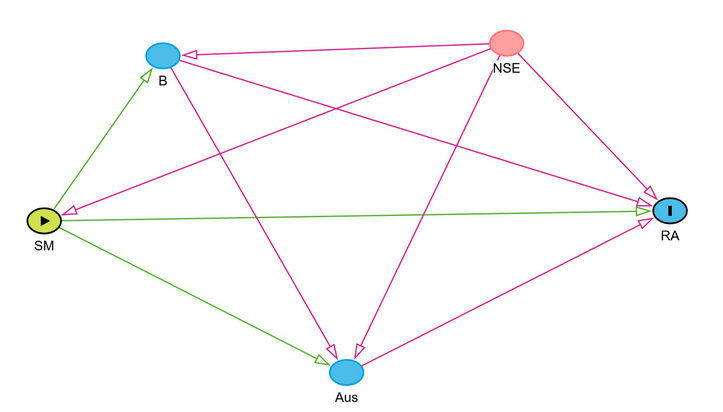
\includegraphics[width=4.16667in,height=\textheight]{./imgs/DAG_ejemplo_2.png}

}

\caption{DAG propuesto.}

\end{figure}

\begin{verbatim}
  a. Describí el DAG completo. Identificá cuál es el camino directo entre SM y RA, y cuáles son las puertas traseras. ¿Cuáles de esas puertas están abiertas?
  b. Identificá todos los caminos causales entre SM y RA, en donde indiques para cada uno si está abierto o cerrado y por qué.
  c. ¿Hay algún *collider* en este DAG? Identificalo y explicá por qué es un *collider* en el contexto de al menos un camino específico. ¿Qué pasaría si el equipo controlara por esa variable?
  d. Aplicando el criterio de las puertas traseras, ¿por qué variables habría que controlar para estimar correctamente el efecto causal de SM sobre RA? Justificá cada decisión.
  e. Escribí el modelo de regresión que deberías ajustar para estimar el efecto causal de interés, según lo que determinaste en la pregunta anterior.
  f. El equipo propone controlar por Aus porque "es una variable importante que afecta el rendimiento". ¿Estás de acuerdo?
\end{verbatim}

\bookmarksetup{startatroot}

\hypertarget{sec-random-exp}{%
\chapter{Experimentos aleatorios}\label{sec-random-exp}}

\hypertarget{por-quuxe9-son-importantes-los-experimentos-aleatorios}{%
\section{¿Por qué son importantes los experimentos
aleatorios?}\label{por-quuxe9-son-importantes-los-experimentos-aleatorios}}

En los experimentos aleatorios\sidenote{\footnotesize A lo largo del capítulo vamos a
  usar de forma intercambiable las expresiones experimentos aleatorios y
  experimentos aleatorizados. También vamos a usar la sigla \textbf{RCT}
  del inglés \emph{randomized controlled trials}.} los sujetos son
asignados a los grupos (por ejemplo, tratamiento y control)
aleatoriamente. Esto significa que en la asignación de los grupos
aleatorios hay involucrado un proceso realmente aleatorio, como arrojar
un moneda. Ojo con confundir el concepto de asignación aleatoria con el
de muestra aleatoria: Que el muestreo sea aleatorio significa que los
participantes son una muestra seleccionada al azar de una población más
amplia, mientras que la asignación aleatoria significa que los
participantes, independientemente de si fueron seleccionados de una
población más amplia o no, son asignados al azar a diferentes
condiciones experimentales.

\begin{tcolorbox}[enhanced jigsaw, breakable, rightrule=.15mm, colbacktitle=quarto-callout-warning-color!10!white, bottomtitle=1mm, arc=.35mm, titlerule=0mm, left=2mm, toprule=.15mm, leftrule=.75mm, colback=white, opacitybacktitle=0.6, opacityback=0, colframe=quarto-callout-warning-color-frame, bottomrule=.15mm, coltitle=black, toptitle=1mm, title={Sobre la aleatoridad de las computadoras}]
Cuando hablamos de un evento aleatorio, hablamos de una entidad
abstracta cuyo resultado no se puede predecir exactamente. Para poner
este tipo de eventos en el mundo real solemos echar mano de ejemplos
clásicos que involucran una complejidad física tal que resulta imposible
predecirlos exactamente, como arrojar un dado o una moneda. El ejemplo
de la moneda es la forma más usual de hablar de una variable aleatoria
con dos posibles valores equiprobables (aunque parezca que no tanto
(Bartoš et~al.
2023)\marginpar{\begin{footnotesize}\leavevmode\vadjust pre{\protect\hypertarget{ref-bartovs2023fair}{}}%
Bartoš, František, Alexandra Sarafoglou, Henrik R Godmann, Amir Sahrani,
David Klein Leunk, Pierre Y Gui, David Voss, et~al. 2023. {«Fair coins
tend to land on the same side they started: Evidence from 350,757
flips»}. \emph{arXiv preprint arXiv:2310.04153}.\vspace{2mm}\par\end{footnotesize}}).
Sin embargo, esta aleatoriedad es muy costosa de reproducir. Es por eso
que las computadores utilizan lo que se llama generadores de números
pseudo aleatorios\sidenote{\footnotesize Para más información pueden ir a leer
  \href{https://en.wikipedia.org/wiki/Pseudorandom_number_generator}{esto}.}.
Estos generadores utilizan series de números generados de forma pseudo
aleatoria pero que puede ser recuperada determinísticamente a partir de
una ``semilla''. Es por eso que cuando simulamos datos en este libro lo
primero que hacemos es ejecutar \texttt{set.seed(42)} (42 o el número
que sea), para de esa forma poder obtener el mismo resultado cada vez
que replicamos, o el lector quiere replicar, las simulaciones.

Dicho esto. A fines prácticos, es totalmente razonable utilizar un
generador de números pseudo aleatorios para la asignación a grupos
experimentales en los experimentos aleatorios.
\end{tcolorbox}

Por ejemplo, en el caso más simple, esto significa que dada una muestra
de personas, vamos a asignar a cada de una de ellas ``tirando una
moneda'' al grupo control (\(D=0\)) o tratamiento (\(D=1\)) como se ve
en la siguiente figura.

\begin{figure}

{\centering 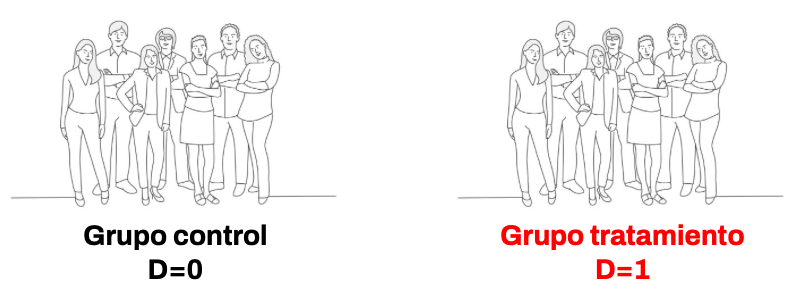
\includegraphics{./imgs/exp_aleatorio.png}

}

\end{figure}

Los experimentos aleatorios son el \emph{gold-standard} para estimar el
efecto de un tratamiento. De hecho, al ser la asignación aleatoria,
podemos asegurar que, como mencionamos en el capítulo
Capítulo~\ref{sec-pot-outcomes}, existe independencia
(\((Y^0, Y^1) \perp D\)). Esto nos asegura que la diferencia de medias
de los grupos tratamiento y control son un estimador consistente del
\textbf{ATE}. Dicho esto, veremos que hay formas más ``eficientes'' de
estimar el \textbf{ATE}, es decir, con mayo potencia estadística.

Hay una razón extra para que en este libro empecemos hablando en detalle
de los experimentos aleatorizados, y es que cuando entremos de lleno en
el mundo de los cuasiexperimentos nos será de gran ayuda entender cuál
es el problema y cuál es la solución que se propone. Esto nos va a
permitir tener una idea más concreta de las ventajas y limitaciones de
cada uno de los diseños cuasiexperimentales que vamos a estudiar más
adelante.

En muchas ocasiones los experimentos aleatorios terminan siendo
degradados a la categoría de cuasiexperimento. Por ejemplo: Supongamos
que hay un estudio que quiere evaluar el efecto de un programa de
\emph{mindfulness} en la cantidad de hechos de violencia en un
establecimiento educativo. Para esto se asigno aleatoriamente a diez
escuelas al grupo \emph{mindfulness} y diez escuelas al grupo control.
Hasta acá todo muy lindo, deberíamos llevar adelante el programa, medir
la cantidad de hechos de violencia en cada escuela, hacer la diferencia
de medias y \emph{voilá}, ya tenemos un estimador del \textbf{ATE}. Pero
a veces las cosas no son tan sencillas y en el medio de este experimento
van a pasar cosas. Por ejemplo, hay un grupo de colegios del grupo
control que, por presión de los padres, incorporan un programa de
\emph{mindfulness} propio, mientras que otro grupo del colegios, esta
vez del grupo tratamiento, deciden no implementar el programa de
\emph{mindfulness} propuesto por nosotros porque les interfiere con la
curricula. Para colmo, varios colegios de ambos grupos deciden que la
participación sea voluntaria. En fin, \textbf{el horror}. Lo que nos
termina pasando es que, aunque el diseño sea un experimento aleatorio,
la pérdida de control sobre la implementación y la participación
voluntaria generan contaminación y sesgo de selección, degradando el
estudio a un cuasiexperimento. Es decir, la comparación entre grupos ya
no se basa en la aleatorización y vamos a requerir de otros controles
estadísticos para corregir posibles sesgos. Más adelante vamos a charlar
un poquito más de esto.

Dicho esto volvamos al maravilloso mundo de los 🌈experimentos
aleatorizados ideales🌈.

\hypertarget{el-experimento-ideal}{%
\section{El experimento ideal}\label{el-experimento-ideal}}

El experimento ideal es ese experimento tan bien planificado, tan bien
implementado y tan bien acatado por sus participantes que en la realidad
nunca ocurre. Sin embargo, hay una excepción y son, en general, los
\emph{medical trials}. De hecho hay algunas características que
esperaríamos ver en un \textbf{RCT}\sidenote{\footnotesize \emph{Randomized clinical
  trials}, o ensayos clínicos aleatorizados. Son estudios experimentales
  que se utilizan para testear la eficacia o la seguridad de
  procedimientos médicos o tratamientos.} y son las siguientes.

\begin{itemize}
\tightlist
\item
  \textbf{Controles adecuados}: Si diseñamos un experimento para estimar
  el efecto de un tratamiento, debemos tener un grupo control adecuado
  con el que comparar. Sin embargo, esto no significa que el \emph{grupo
  control} sea siempre un grupo simplemente no expuesto al tratamiento.
  Por ejemplo, es muy conocido el ejemplo de la determinación de la
  efectividad de un fármaco, en los que al \emph{grupo control} se le
  ofrece una pastilla que no contiene a la droga siendo estudiada sino
  unas pastilla de igual forma, tamaño y prescripción de consumo pero,
  típicamente, de azucar. Esto lo que nos permite es poder descontar el
  efecto de consumir un placebo en la estimación final de la efectividad
  del fármaco\sidenote{\footnotesize Si les interesa, también existen el efecto
    \href{https://pmc.ncbi.nlm.nih.gov/articles/PMC4804316/}{nocebo} y
    \href{https://themicrodose.substack.com/p/the-power-of-know-cebo-5-questions?publication_id=371945\&post_id=159587451\&isFreemail=true\&r=3zjda\&triedRedirect=true}{\emph{know-cebo}}.}.También
  es posible que por consideraciones éticas no podamos dejar al grupo
  control con un tratamiento placebo (por ejemplo cuando ya existe un
  tratamiento efectivo para la enfermedad que estamos estudiando, si lo
  hicieramos privaríamos a los sujetos del grupo control de su derecho a
  la salud), en estos casos el \emph{grupo control} recibe el
  tratamiento típico y el \emph{grupo tratamiento} el del estudio, en
  estos casos descontaremos el efecto del tratamiento común y nuestro
  ATE es el efecto de la intervencion \emph{por encima del tratamiento
  usual}
\end{itemize}

\begin{itemize}
\item
  \textbf{Asignación aleatoria a los grupos experimentles}: Como vimos
  en el capítulo Capítulo~\ref{sec-pot-outcomes}, la mejor forma de
  asegurar que los grupos control y tratamiento son lo más iguales
  posibles es asignando aleatoriamente a los participantes. Esto, junto
  con una cantidad de participantes suficiente nos asegura que ambos
  grupos son iguales en todos los factores que pueden influenciar el
  resultado del experimento, incluyendo los factores de los que no
  sabemos.
\item
  \textbf{Los individuos deben ser considerados en el grupo asignado}:
  Los participantes asignados al grupo tratamiento deben ser
  considerados como tratamiento, independientemente de si se expusieron
  o no al mismo. Esto es conocido como el principio \emph{intention to
  treat} y puede sonar un poco raro. Sin embargo, lo podemos pensar como
  un cambio del tratamiento que queremos evaluar. Por ejemplo, hay un
  experimento en el que se quiere evaluar el efecto de la estatinas en
  el colesterol LDL. Hay un grupo al que le dan estatinas y otro grupo
  al que le dan un placebo. Un \$18\% \$ de los que fueron originalmente
  asignados al grupo estatinas dejó de tomarlas y un \$38\% \$ de los
  que fueron asignados al grupo placebo empezó a tomar estatinas durante
  el trial. Esto significa que nuestro experimento no estimaría
  correctamente el efecto de \emph{tomar} las estatinas, pero por otro
  lado, sí estimaría bien el efecto de \emph{ser recetado} con
  estatinas. Y si lo pensamos un poco: ¿No es algo más razonable estimar
  el efecto de lo segundo?\sidenote{\footnotesize Una mejor explicación de este
    enfoque y su contraparte (no recomendada), el análisis por protocolo
    pueden visitar este paper{[}esto{]}
    https://onlinelibrary.wiley.com/doi/10.1111/nep.13709}
\end{itemize}

\begin{itemize}
\item
  \textbf{Todos los grupos deben ser tratados igual}: Por ejemplo, si en
  el ejemplo anterior invitamos a la gente del grupo de estatinas a
  controles médicos más seguidos, o los evaluamos con más dedicación, va
  a ser imposible separar los beneficios de la droga de los beneficios
  de las diferencias en cómo tratamos a los pacientes.
\item
  \textbf{Blinded}: Para que las estimaciones de un experimento no se
  contaminen, resulta necesario que los participantes (o unidad
  experimental) no conozcan a que grupo experimental pertenecen. Esto es
  importante porque podría haber algún tipo de contaminación del efecto
  como por ejemplo que los sujetos que sepan que reciben la intervención
  se esfuercen para rendir mejor en el outcome o lo contrario al saberse
  ``abandonados'' al grupo control tiendan a rendir peor.
\item
  \textbf{Double blinded}: Siguiendo con lo mencionado antes, también
  resulta deseable que los investigadores tampoco sepan a que grupo
  experimental pertenece un sujeto o unidad experimental. Esto tiene
  como objetivo reducir al mínimo las diferencias entre los grupos. Por
  ejemplo, en un experimento para estimar la efectividad de una campaña
  de comunicación para motivar la vacunación, los investigadores podrían
  espaciar menos las comunicaciones con alguno de los grupos
  experimentales, contaminando así el efecto de la intervención en sí
  misma.

  Por supuesto que esto no siempre es posible. Por ejemplo, si un
  experimento quiere estimar la efectividad de una nueva cirujía
  laparoscopica versus su alternativa tradicional, resulta imposible que
  el cirujano que va a llevar adelante la misma no sepa a qué grupo
  pertenece el paciente. Sin embargo, es importante que en estos casos
  la asignación al grupo se retrase lo más posible disminuyendo la
  posible influencia de otros participantes (por ejemplo, un
  investigador podría estar más atento a la preparación preoperatoria de
  algún grupo experimental).
\item
  \textbf{Medir a todos los individuos}: Todos los individuos que
  comenzaron el experimento deben ser medidos para evaluar el efecto del
  tratamiento. Esto no siempre pasa y es algo de lo que vamos a hablar
  más adelante en este capítulo.
\end{itemize}

Que lindo es el diseño experimental. Todos somos felices, todo funciona.
¿El libro debería terminar acá?

\begin{figure}

{\centering 
\includegraphics[width=0.5\textwidth,height=\textheight]{./imgs/abogados.jpeg}

}

\end{figure}

Pues no mi ciela. Ojalá llevar adelante experimentos fuera tan fácil.

\hypertarget{cuando-la-cosa-no-es-tan-ideal}{%
\section{Cuando la cosa no es tan
ideal}\label{cuando-la-cosa-no-es-tan-ideal}}

\hypertarget{aleatorizaciuxf3n-por-bloques}{%
\subsection{Aleatorización por
bloques}\label{aleatorizaciuxf3n-por-bloques}}

Intuitivamente pensamos que la aleatorizacion de los sujetos a un grupo
control o un grupo tratamiento es tan simple como lanzar una moneda (y
muchas veces lo es), este método se conoce como \textbf{aletorización
simple}. Sin embargo puede que este método no sea siempre deseado. Por
ejemplo, se quiere testear la ventaja de una intervención laparoscópica
(mínimamente invasiva) sobre una cirugía tradicional (en la que se abre
el abdomen). Es razonable pensar que los cirujanos se vuelven mejores
con el tiempo sin importar a que tipo de cirugía, porque la práctica
hace al maestro. Bueno imaginemos que aplicamos un proceso de
aleatorización simple, es posible que los primeros sujetos sean
asignados con más frecuencia al grupo tratamiento que al grupo control y
los últimos viceversa (ya que la randomizacion es un proceso
independiente, la asignación del sujeto anterior no condiciona al que
sigue, y esto es posible). En este escenario hipotetico pero posible, el
ATE que queremos estimar se encuentra contaminado por una variable
confusora (la habilidad del cirujano). ¿Cómo evitamos esto? Bueno una
forma razonable es evitar que los sujetos se asignen al grupo todos
juntos sino a medida que el cirujano va \emph{aprendiendo}. Para hacer
esto se pueden crear bloques temporales, por ejemplo, los 10 primeros
voluntarios, los 10 siguientes y así sucesivamente. Dentro de cada
bloque hacemos una asignación aleatoria, de esta forma nos aseguramos
que haya un numero mas o menos balanceado de sujetos en el grupo control
e intervencion expuestos al cirujano torpe, intermedio y master level.

\begin{figure}

{\centering 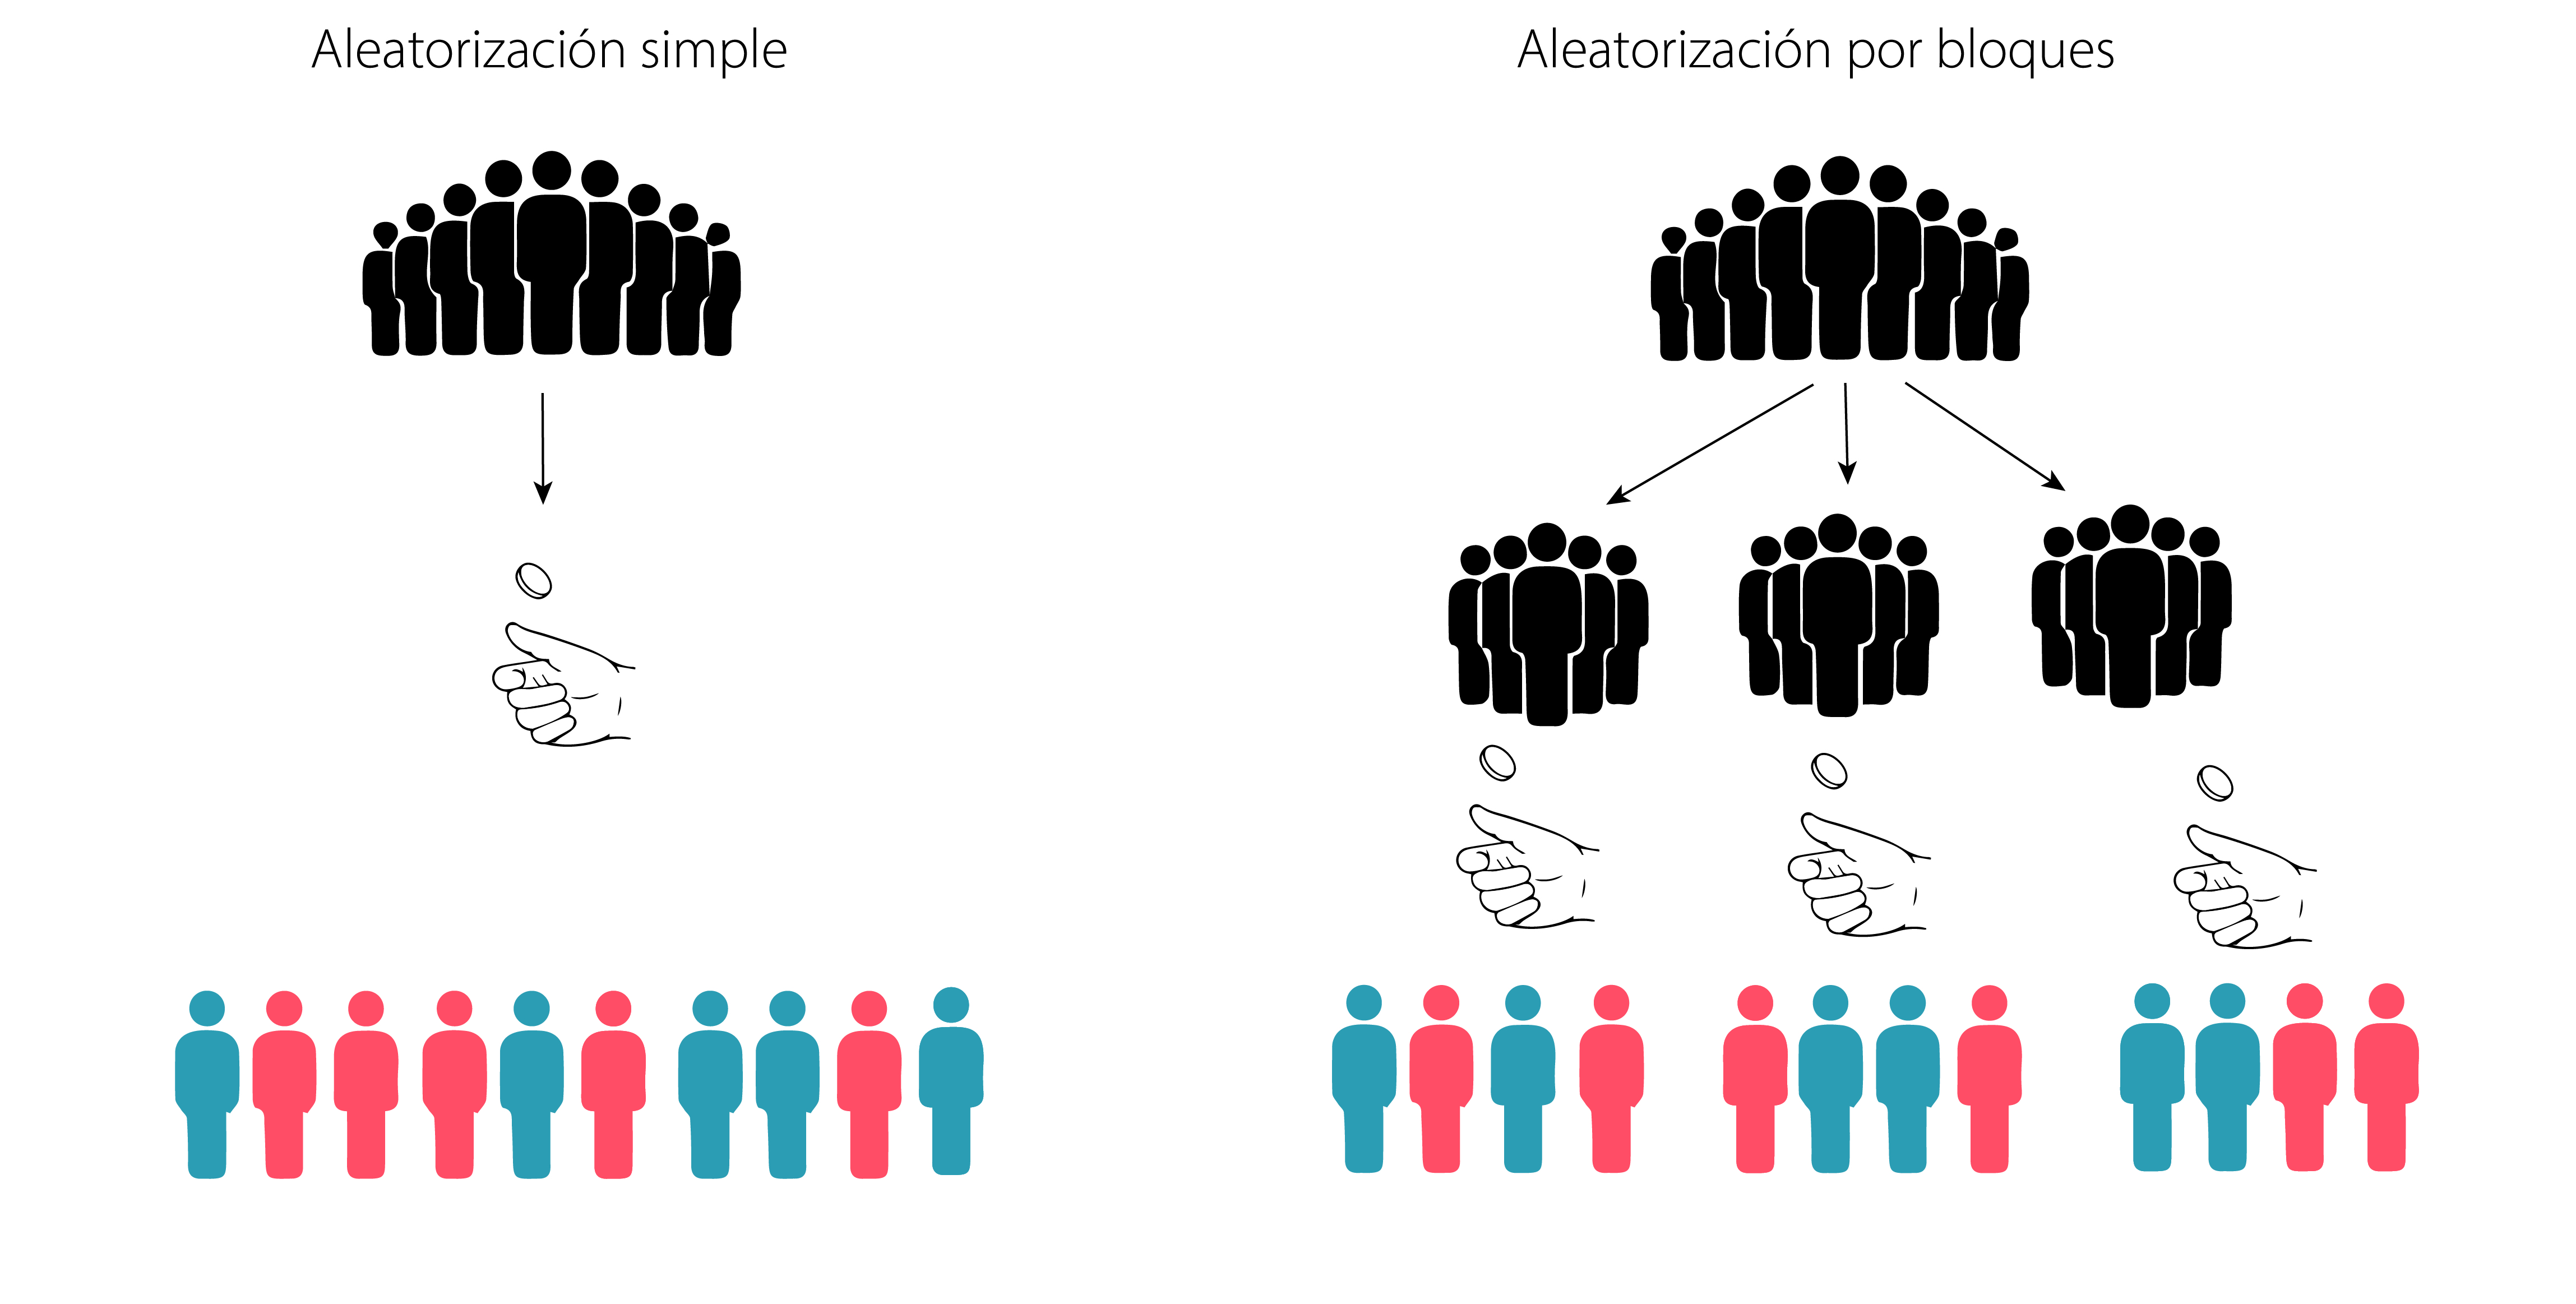
\includegraphics{./imgs/block_aleatorizacion.jpg}

}

\end{figure}

\hypertarget{spillover}{%
\subsection{\texorpdfstring{\emph{Spillover}}{Spillover}}\label{spillover}}

En un experimento ideal, los sujetos son asignados aletoriamente a los
grupos experimentales \textbf{y se quedan ahí}. El efecto
\emph{spillover} o derrame sucede cuando los sujetos del grupo control
reciben en forma indirecta parte o todo el tratamiento que esta diseñado
para el grupo de intervención. ¿Cómo es esto posible? Es muy posible,
sobre todo en intervenciones conductuales. Pongamos ejemplos para que se
entienda. Supongamos que queremos ver el efecto de una intervención
educativa como hábitos saludables para prevenir cierta enfermedad,
algunos sujetos son asignados a la intervención y reciben una charla
educativa y otros nada. Un par de amigos (\emph{i} y \emph{j}) han sido
aleatorizados a un grupo y al otro respectivamente. Al terminar la
intervención el sujeto intervenido (\emph{i}) le cuenta la charla al
sujeto del grupo control (\emph{j}) y este ``recibe el tratamiento''. En
este ejemplo un sujeto asignado a un grupo control recibe el tratamiento
destinado al grupo intervención. Es decir, el grupo tratamiento \emph{ha
derramado} hacia el grupo control.

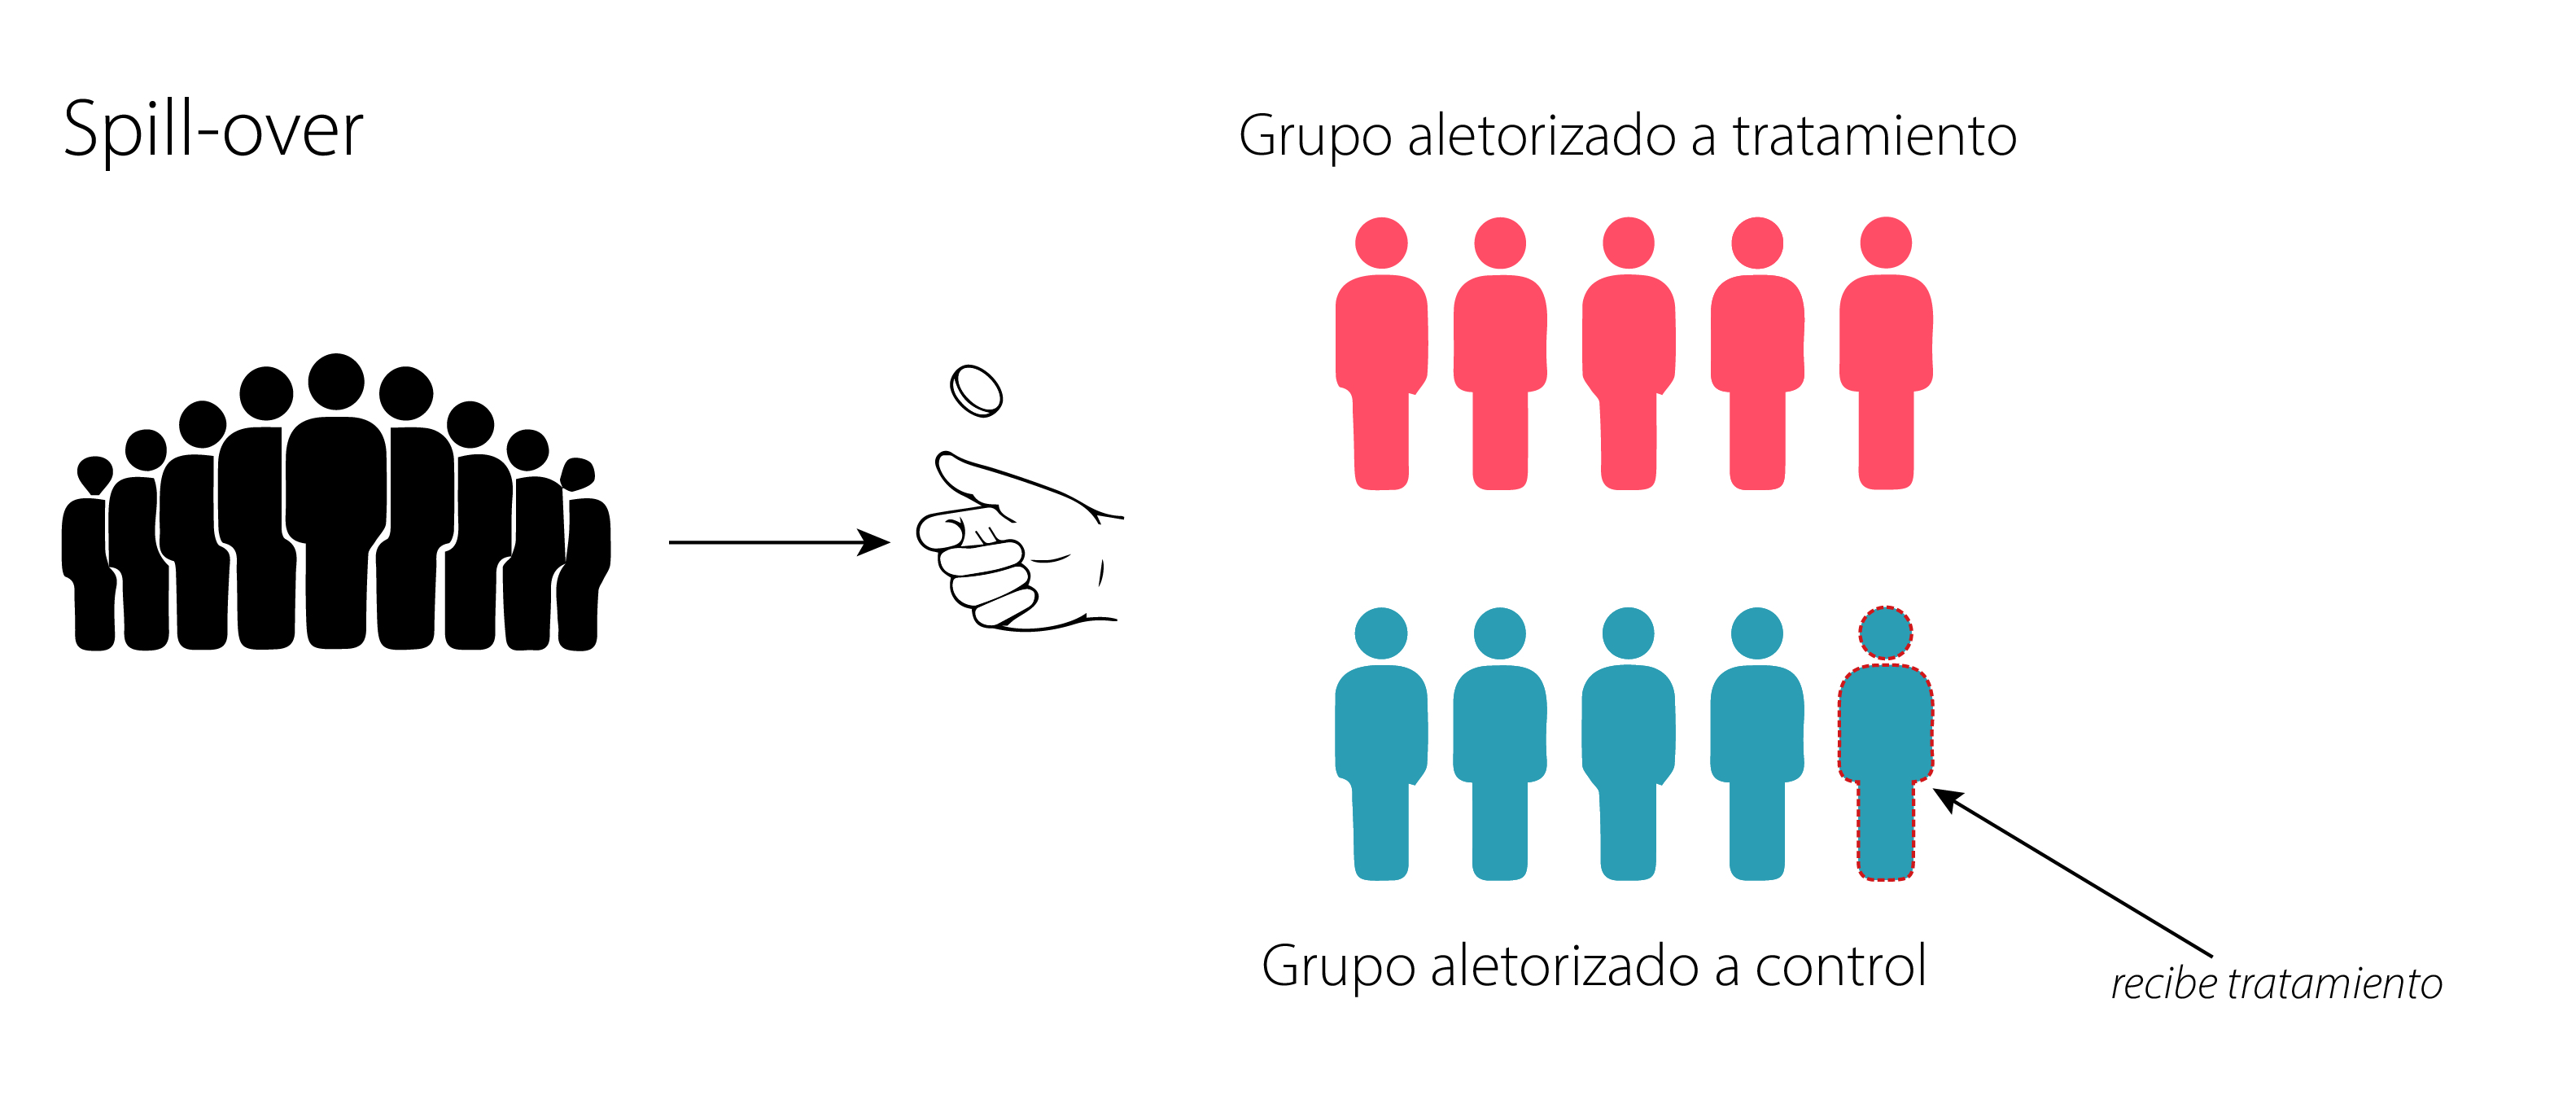
\includegraphics{./imgs/spillover.jpg}

Vale la pena preguntarse por qué el spillover es relevante en los
estudios aleatorizados. Si volvemos al capítulo 3 y a repasar outcomes
potenciales podemos ver que este marco requiere una asuncion a la que
llamamos \textbf{SUTVA}\sidenote{\footnotesize Del inglés \emph{stable unit treatment
  value assumption}.} o en otras palabras este supuesto establece que
los resultados potenciales del sujeto \emph{j} dependen únicamente de su
propio estado de tratamiento (el que fue asignado), sin verse afectados
por el tratamiento recibido por otro sujeto \emph{i}. Sin embargo esto
no es así, ya que \emph{i} es responsable del resultado potencial de
\emph{j} porque ``le ha aplicado'' el tratamiento. Al violar esta
asunción, estimar el \textbf{ATE} a través de una diferencia de medias
puede estar francamente sesgado por este efecto. El spillover es un
efecto difícil de rastrear y sobretodo difícil de corregir, es frecuente
en intervenciones que tienen que ver con comunicacion o informacion, ya
que la comunicación fluye despues de la intervención de forma
incontrolable para los investigadores. El mejor enfoque es preveer esta
posibilidad e instaurar barreras a priori para disminuir el contagio que
una intervención pueda tener sobr el grupo control.

\hypertarget{reversiuxf3n-de-la-cadena-causal-o-reverse-causation}{%
\subsection{\texorpdfstring{Reversión de la cadena causal (o
\emph{reverse
causation})}{Reversión de la cadena causal (o reverse causation)}}\label{reversiuxf3n-de-la-cadena-causal-o-reverse-causation}}

La reversión causal es uno de los sesgos que pueden plagar nuestra
interpretación de la cadena causa-efecto, sobre todo en los estudios
observacionales.

Inventemos un escenario hipotético: pensemos que un investigador quiere
evaluar si la lluvia caída aumenta la frecuencia de gente con paragüas
en la calle. La respuesta es obvia para nosotros que conocemos las leyes
de la naturaleza y que la gente odia mojarse. Cada vez que llueve, la
gente sale a la calle con paragüas. Pero que pasa si nuestro
investigador fuera un ser completamente ajeno a todo esto (digamos un
batiduende de la 5ta dimensión) y no tuviera conocimiento alguno previo.
Este ser, podría contar la frecuencia de paraguas en la calle y si
llueve o no, hacer una regresión logística (por poner un ejemplo) para
predecir la lluvia en función de la cantidad de paragüas de la calle y
de seguro que sería un predictor significativo. Y es más, podría cerrar
su estudio concluyendo que un aumento de una unidad en la frecuencia de
paragüas aumenta en un cierto porcentaje las chances de que llueva, o
sea que los paragüas \emph{causan} la lluvia. Nuestro batiduende
investigador habría incurrido en un \textbf{sesgo de causalidad
inversa}. Podríamos pensar por lo absurdo del ejemplo que este sesgo es
difícil de que afecte a nuestras investigaciones, sin embargo es muy
frecuente. Ejemplos de causalidad reversa son por ejemplo: observar que
los barrios con propiedades mas costosas tienen un centro comercial y
suponer que colocar un centro comercial en un barrio aumenta el valor de
la vivienda, cuando lo que pasa es que los centros comerciales decidan
colocarse en barrios con propiedades costosas; u observar que las
personas que hacen más ejercicio tienen menos síntomas depresivos, e
interpretar que hacer ejercicio reduce la depresión cuando podría ser
que las personas menos deprimidas tienen más energía o motivación para
hacer ejercicio.

Los diseños experimentales pueden protegernos mejor que los estudios
observacionales de este tipo de sesgo, por qué, fundamentalmente porque
en nuestro diseño experimental vamos a \emph{aplicar} la causa y esperar
que la consecuencia suceda después de esto. Por regla general las causas
no pueden ocurrir después que sus consecuencias y de esta manera la
dirección de la causalidad es forzada hacia un solo lado. Sin embargo,
el sesgo de causalidad inversa puede ocurrir aún así en un ensayo
experimental bajo ciertas condiciones:

\begin{itemize}
\item
  \textbf{No cumplimiento del tratamiento (non-compliance)}: Supongamos
  que en el experimento se asigna aleatoriamente a algunos sujetos a
  recibir un tratamiento, por ejemplo una nueva terapia para la caida de
  cabello, pero los sujetos con mas caida de cabello en las primeras
  dosis del grupo tratamiento sienten que el tratamiento es inutil y
  dejan de tomar las pastillas . Este evento introduce un sesgo de
  causalidad inversa si analizamos a los sujetos por si tomaron el
  tratamiento o no (por protocolo en lugar de intention-to-treat) ya que
  el outcome (la caida del cabello) genera la exposición (la cantidad de
  medicación que las personas en el grupo de tratamiento reciben.
\item
  \textbf{Efectos anticipados o comportamiento reactivo}: A veces, los
  participantes modifican su comportamiento en respuesta a saber su
  asignación. Ejemplo: alguien asignado al grupo control empieza a
  buscar alternativas por su cuenta (porque no recibió tratamiento), y
  eso afecta su resultado. O alguien en el grupo tratado ya anticipa que
  tendrá mejoría y cambia su comportamiento desde antes del tratamiento
  real. El resultado cambia en respuesta a la expectativa del
  tratamiento, y no necesariamente al tratamiento en sí.
\item
  \textbf{Mediciones mal temporizadas}: En algunos experimentos, puede
  que la variable de outcome sea medida antes de que el tratamiento
  surta efecto, o incluso antes de aplicarlo bien. Si los resultados se
  usan para definir o cambiar el tratamiento asignado (por error o por
  diseño), ya no hay garantía de temporalidad: el resultado podría estar
  influyendo en el tratamiento.
\end{itemize}

\begin{tcolorbox}[enhanced jigsaw, breakable, rightrule=.15mm, colbacktitle=quarto-callout-warning-color!10!white, bottomtitle=1mm, arc=.35mm, titlerule=0mm, left=2mm, toprule=.15mm, leftrule=.75mm, colback=white, opacitybacktitle=0.6, opacityback=0, colframe=quarto-callout-warning-color-frame, bottomrule=.15mm, coltitle=black, toptitle=1mm, title={Advertencia}]
Si prestaron atención a las secciones anteriores sospecharan que muchos
de estos sesgos de causalidad inversa puedan evitarse aplicando analisis
ITT y asegurandonos un blinded adecuado, es así
\end{tcolorbox}

\hypertarget{experimentos-between-groups}{%
\section{\texorpdfstring{Experimentos \emph{between
groups}}{Experimentos between groups}}\label{experimentos-between-groups}}

\begin{tcolorbox}[enhanced jigsaw, breakable, rightrule=.15mm, colbacktitle=quarto-callout-warning-color!10!white, bottomtitle=1mm, arc=.35mm, titlerule=0mm, left=2mm, toprule=.15mm, leftrule=.75mm, colback=white, opacitybacktitle=0.6, opacityback=0, colframe=quarto-callout-warning-color-frame, bottomrule=.15mm, coltitle=black, toptitle=1mm, title={Hablemos un poco de la nomenclatura}]

\end{tcolorbox}

En este capítulo definimos los experimentos aleatorizados como aquellos
en los que se asigna al azar a los participantes a una condición de
tratamiento o de control. Este enfoque corresponde, en realidad a un
sólo tipo de diseño aletorizado, los diseños conocidos como
\textbf{between-groups}.

En los experimentos \textbf{between-groups}, \emph{los participantes se
distribuyen aleatoriamente entre diferentes condiciones de tratamiento,
formando grupos que luego se comparan entre sí}. Por ejemplo, se puede
asignar a estudiantes a distintos métodos de enseñanza, a pacientes
hipertensos a planes de dieta variados o a adultos mayores a programas
de ejercicio físico.

Antes de analizar los distintos tipos de diseños dentro de esta
categoría, presentaremos algunas \textbf{definiciones y notaciones
clave.}

Cuando querramos representar esquematicamente un diseño, vamos a
recurrir a la notación clásica. Según esta, se representarán
gráficamente tanto los experimentos aleatorizados como los
cuasi-experimentos usando las letras \(X\) y \(O\). Una \(X\) indica la
administración de un tratamiento, y una \(O\) representa una
observación. Una \(O\) puede referirse a una observación de una o varias
variables en un momento determinado. Una observación puede ser cualquier
tipo de medición, ya sea un test escrito, un registro fisiológico, un
informe verbal, o cualquier otra evaluación empírica. En estos
diagramas, el tiempo (como la lectura) fluye de izquierda a derecha.
Cuando se realizan varias observaciones, se utilizan \textbf{subíndices}
en las \(O\) para indicar el momento de cada medición.

Utilizando esta notación, el experimento aleatorizado entre grupos más
simple se representa así:

\hfill\break

\begin{array}{lcl}
\text{R:} & X & O \\
\text{R:} &   & O \\
\end{array}

\hfill\break

Vamos a tratar de entender que significa esta notación, en principio hay
dos líneas, esto indica que hay dos grupos, cada línea empieza con una
\(R\), esto indica que los sujetos fueron asignados aleatoriamente (o
random) a la participacion de ese grupo, vemos en la primera línea que
ese grupo a recibido un tratamiento \(X\) y el otro no y que ambos
grupos han sido evaluados posterior a ello en una instancia \(O\). Este
diseño se conoce como \textbf{post-test only} o \textbf{sólo post-test}
ya que como puede verse en este diseño la única medida que se toma es
despues de la intervención.

Una vez que hemos entendido este diseño sencillo podemos introducir otro
un poco más complejo como este

\begin{array}{lcl}
\text{R:}& O_1 & X & O_2 \\
\text{R:}& O_1 &   & O_2 \\
\end{array}

La fila superior indica que un grupo es observado (\(O_1\)), luego
recibe un tratamiento (\(X\)), y se observa nuevamente (\(O_2\)). La
fila inferior muestra que un segundo grupo es observado, no recibe el
tratamiento (aunque puede recibir uno alternativo), y luego es observado
de nuevo. Nuevamente, la ``\(R:\)'' indica asignación aleatoria. (Lo
ideal es realizar la asignación aleatoria después de la \(O_1\), así que
la posición de ``\(R:\)'' no indica necesariamente el orden temporal, ya
discutiremos el por qué de esto). En pocas palabras lo que diferencia
este diseño del anterior es que existe una observación más, una antes de
la intervención. Este tipo de diseño entonces se llama
\textbf{pretest-posttest}. Ahora que hemos introducido esquemáticamente
los dos diseños fundamentales de los experimentos aleatorizados entre
grupos vamos a hablar de ello.

\hypertarget{suxf3lo-posttest}{%
\subsection{\texorpdfstring{Sólo
\emph{posttest}}{Sólo posttest}}\label{suxf3lo-posttest}}

Recapitulemos, los diseños post-test only son la forma más simple de
experimentos aletorizados entre grupos en donde un grupo es
aleatoriamente asignado a una intervención, el otro a su condición de
control, y posteriormente a ello se evalua el outcome. Resumiendo e la
notación:

\begin{array}{lcl}
\text{R:} & X & O \\
\text{R:} &   & O \\
\end{array}

Este diseño puede escribirse (y analizarse) utilizando un modelo lineal
que tiene la siguiente forma:

\begin{equation}\protect\hypertarget{eq-postest_model}{}{
\begin{array}
_Y_{i} &=& \beta_0 + \beta_T T_i + \epsilon_{i}
\end{array}
}\label{eq-postest_model}\end{equation}

Donde \(Y_i\) es el valor de que adopta \(O\) (es decir nuestro outcome
post-intervención), y \(T_i\) es una variable indicadora que toma el
valor \(1\) si el participante pertenece al grupo tratamiento y el valor
\(0\) si no y \(\epsilon_{i}\) representa el término de error (varianza
no explicada por el modelo). Para los modelos que veamos en estas
secciones \(\epsilon_{i}\) tiene una distribución
\(\epsilon_{i} \sim \mathcal{N}(0, \sigma_\epsilon^2)\),

Vamos a ver como podemos usar este diseño (y este modelo), para estimar
el \textbf{ATE}.

\hypertarget{un-ab-test}{%
\subsubsection{Un A/B test}\label{un-ab-test}}

Un \textbf{A/B test} es un experimento aletorizado muy popular en el
campo del diseño de páginas web. El mismo consiste en presentar a los
usuarios con dos versiones del mismo sitio web (la versión A y la
versión B) y medir su comportamiento en función de la versión que se les
presenta. Por ejemplo, se puede medir el tiempo que los usuarios pasan
en el sitio web, la tasa de clics en un botón o cualquier otra métrica
relevante. La idea es comparar el rendimiento de las dos versiones para
determinar cuál es más efectiva.

En nuestro ejemplo vamnos a asignar aleatoriamente a los usuarios a dos
versiones distintas de un sitio web (la version anterior \textbf{Website
A} o control, y la version nueva \textbf{Website B} o intervención) y
mediremos el tiempo de permanencia en segundos. Es decir, queremos ver
si el cambio de diseño de la página web tiene un efecto positivo en el
tiempo que los usuarios pasan en el sitio. En este caso, el tiempo de
permanencia es nuestro outcome y la variable de tratamiento es la
versión del sitio web.

Vamos a simular los datos para \(100\) usuarios (50 en cada grupo) y
luego vamos a estimar el \textbf{ATE} usando un modelo lineal. Como los
datos son simulados, conocemos el efecto real de la intervención (el
\textbf{ATE}) que es de \(5\) segundos. De hecho, sabemos que el tiempo
promedio de permanencia en la versión A es de \(50\) segundos y en la
versión B es de \(55\) segundos \sidenote{\footnotesize ¿Por qué decimos que la
  asignación es aleatoria si en ningún momento tiramos una moneda?
  Bueno, si miran el código que utilizamos para la simulación de los
  datos, vamos a ver que los tiempos base (antes de sumar el
  tratamiento, \(\beta_0 + \epsilon_{i}\) en nuestro modelo) son
  muestras de una \(\mathcal{N}(50, 10^2)\), es decir, una normal con
  media \(50\) y desviación estándar \(10\). Luego asignamos la mitad
  para el grupo control y la mitad para el grupo tratamiento (a los que
  les sumamos \(\beta_T\)). Como nuestros sujetos no tienen una
  ``identidad'', al separar mitad para cada lado dado que son muestras
  aleatorias tomadas de una distribución es como si estuviéramos
  asignando aleatoriamente a los grupos experimentales.}.

\begin{Shaded}
\begin{Highlighting}[]
\FunctionTok{set.seed}\NormalTok{(}\DecValTok{42}\NormalTok{)}
\CommentTok{\# Simulamos el experimento}
\NormalTok{n }\OtherTok{\textless{}{-}} \DecValTok{50} \CommentTok{\# Sujetos por condición}
\NormalTok{t }\OtherTok{\textless{}{-}} \FunctionTok{rnorm}\NormalTok{(}\DecValTok{2}\SpecialCharTok{*}\NormalTok{n, }\DecValTok{50}\NormalTok{, }\DecValTok{10}\NormalTok{) }\CommentTok{\# Variable que indica la exposición al tratamiento}
\NormalTok{t\_control }\OtherTok{\textless{}{-}}\NormalTok{ t[}\DecValTok{1}\SpecialCharTok{:}\NormalTok{n] }\CommentTok{\# Tiempos del grupo control}
\NormalTok{t\_tratamiento }\OtherTok{\textless{}{-}}\NormalTok{ t[(n}\SpecialCharTok{+}\DecValTok{1}\NormalTok{)}\SpecialCharTok{:}\NormalTok{(}\DecValTok{2}\SpecialCharTok{*}\NormalTok{n)] }\SpecialCharTok{+} \DecValTok{5} \CommentTok{\# Tiempos del grupo tratamiento}

\NormalTok{data }\OtherTok{\textless{}{-}} \FunctionTok{tibble}\NormalTok{(}\AttributeTok{tiempo =} \FunctionTok{c}\NormalTok{(t\_control, t\_tratamiento),}
               \AttributeTok{condicion =} \FunctionTok{c}\NormalTok{(}\FunctionTok{rep}\NormalTok{(}\StringTok{"Website A"}\NormalTok{, n), }\FunctionTok{rep}\NormalTok{(}\StringTok{"Website B"}\NormalTok{, n)))}

\NormalTok{data }\SpecialCharTok{|\textgreater{}}
  \FunctionTok{ggplot}\NormalTok{(}\FunctionTok{aes}\NormalTok{(}\AttributeTok{x =}\NormalTok{ condicion, }
             \AttributeTok{y =}\NormalTok{ tiempo, }
             \AttributeTok{color =}\NormalTok{ condicion)) }\SpecialCharTok{+}
  \FunctionTok{geom\_jitter}\NormalTok{(}\AttributeTok{width =}\NormalTok{ .}\DecValTok{2}\NormalTok{) }\SpecialCharTok{+} 
  \FunctionTok{scale\_color\_manual}\NormalTok{(}\AttributeTok{values =} \FunctionTok{c}\NormalTok{(}\StringTok{"\#1380A1"}\NormalTok{, }\StringTok{"\#ED6A5A"}\NormalTok{)) }\SpecialCharTok{+}
  \FunctionTok{labs}\NormalTok{(}\AttributeTok{x =} \ConstantTok{NULL}\NormalTok{,}
       \AttributeTok{y =} \StringTok{"Tiempo (s)"}\NormalTok{, }
       \AttributeTok{color =} \ConstantTok{NULL}\NormalTok{) }\SpecialCharTok{+}
  \FunctionTok{theme\_bw}\NormalTok{() }\SpecialCharTok{+}
  \FunctionTok{theme}\NormalTok{(}\AttributeTok{legend.position =} \StringTok{"top"}\NormalTok{)}
\end{Highlighting}
\end{Shaded}

\begin{figure}[H]

{\centering 
\includegraphics[width=18.75in,height=\textheight]{./exp_aleatorios_files/figure-pdf/unnamed-chunk-2-1.pdf}

}

\end{figure}

En nuestro caso la versión del modelo de la ecuación
Ecuación~\ref{eq-postest_model} es la siguiente:

\[
\begin{array}
_t_{i} &=& \beta_0 + \beta_T T_i + \epsilon_{i}
\end{array}
\]

Donde \(t_i\) es el tiempo de permanencia en segundos, y \(T_i\) es una
variable indicadora que toma el valor \(1\) si el participante pertenece
al grupo tratamiento (\textbf{Website B}) y el valor \(0\) si pertenece
al grupo control (\textbf{Website A}). En este caso, \(\beta_T\)
representa la diferencia promedio entre los dos grupos, es decir, el
\textbf{ATE}.

Ajustemos un modelo lineal y veamos cómo da la cosa.

\begin{Shaded}
\begin{Highlighting}[]
\NormalTok{model\_postets\_only }\OtherTok{\textless{}{-}} \FunctionTok{lm}\NormalTok{(}\AttributeTok{data =}\NormalTok{ data, tiempo }\SpecialCharTok{\textasciitilde{}}\NormalTok{ condicion, }\AttributeTok{model =}\NormalTok{ T)}
\FunctionTok{modelsummary}\NormalTok{(}\FunctionTok{list}\NormalTok{(}\StringTok{"A/B Postest only"}\OtherTok{=}\NormalTok{ model\_postets\_only),}
             \AttributeTok{coef\_rename =} \FunctionTok{c}\NormalTok{(}\StringTok{"condicionWebsite B"} \OtherTok{=} \StringTok{"Website B"}\NormalTok{),}
             \AttributeTok{statistic =} \FunctionTok{c}\NormalTok{(}\StringTok{"Error estándar = \{std.error\}"}\NormalTok{),}
             \AttributeTok{gof\_omit =} \StringTok{".*"}\NormalTok{,)}
\end{Highlighting}
\end{Shaded}

\begin{table}
\centering
\begin{tblr}[         %% tabularray outer open
]                     %% tabularray outer close
{                     %% tabularray inner open
colspec={Q[]Q[]},
column{2}={}{halign=c,},
column{1}={}{halign=l,},
}                     %% tabularray inner close
\toprule
& A/B Postest only \\ \midrule %% TinyTableHeader
(Intercept) & \num{49.643} \\
& Error estándar = \num{1.477} \\
Website B & \num{6.364} \\
& Error estándar = \num{2.089} \\
\bottomrule
\end{tblr}
\end{table}

Como podemos ver, la estimación del efecto del tratamiento es de 6.36
segundos. Esto significa que la nueva versión del sitio web tiene un
efecto positivo en el tiempo de permanencia de los usuarios en
comparación con la versión anterior.

¿Pero no era que el efecto real era de \(5\) segundos y que el
\(\hat\beta_T\) era un estimador insesgado del efecto porque se trata de
un experimento aleatorio?\sidenote{\footnotesize No confundamos esa diferencia de 1.36
  con un sesgo como el que vimos en el capítulo
  {[}\#sec-pot-outcomes{]}. En ese caso recordemos que había esperanzas
  involucradas.} La respuesta es simple y complicada al mismo tiempo. Al
simular los datos del experimento estamos tomando una muestra aleatoria
y este \(\hat\beta_T\) no es más que una estimación, es decir, una
realización. Esto tiene que ver con que si bien el parámetro \(\beta_T\)
vale \(5\) sus estimaciones no son siempre exactamente \(5\). Lo que si
nos asegura el experimento aleatorizado es que el estimador
\(\hat\beta_T\) es un estimador insesgado del parámetro \(\beta_T\). Es
decir, si repitiéramos el experimento muchas veces, la media de todas
las estimaciones \(\hat\beta_T\) sería igual a \(5\).

Como simulamos los datos, podemos simular \(1000\) realizaciones del
experiento y ver qué pinta tiene esto, ¿No?

\begin{Shaded}
\begin{Highlighting}[]
\CommentTok{\# Simulemos mil experimentos}

\FunctionTok{set.seed}\NormalTok{(}\DecValTok{42}\NormalTok{)}
\CommentTok{\# Simulamos el experimento}
\NormalTok{n }\OtherTok{\textless{}{-}} \DecValTok{50} \CommentTok{\# Sujetos por condición}

\NormalTok{betapostest }\OtherTok{\textless{}{-}} \FunctionTok{c}\NormalTok{()}
\NormalTok{beta\_T }\OtherTok{\textless{}{-}} \DecValTok{5}
\NormalTok{d }\OtherTok{\textless{}{-}} \FunctionTok{c}\NormalTok{(}\FunctionTok{rep}\NormalTok{(}\StringTok{"Website A"}\NormalTok{, n), }\FunctionTok{rep}\NormalTok{(}\StringTok{"Website B"}\NormalTok{, n))}

\ControlFlowTok{for}\NormalTok{ (i }\ControlFlowTok{in} \DecValTok{1}\SpecialCharTok{:}\DecValTok{1000}\NormalTok{) \{}
\NormalTok{  t }\OtherTok{\textless{}{-}} \FunctionTok{rnorm}\NormalTok{(}\DecValTok{2}\SpecialCharTok{*}\NormalTok{n, }\DecValTok{50}\NormalTok{, }\DecValTok{10}\NormalTok{) }\CommentTok{\# Variable que indica la exposición al tratamiento}
\NormalTok{  t\_control }\OtherTok{\textless{}{-}}\NormalTok{ t[}\DecValTok{1}\SpecialCharTok{:}\NormalTok{n] }\CommentTok{\# Tiempos del grupo control}
\NormalTok{  t\_tratamiento }\OtherTok{\textless{}{-}}\NormalTok{ t[(n}\SpecialCharTok{+}\DecValTok{1}\NormalTok{)}\SpecialCharTok{:}\NormalTok{(}\DecValTok{2}\SpecialCharTok{*}\NormalTok{n)] }\SpecialCharTok{+}\NormalTok{ beta\_T }\CommentTok{\# Tiempos del grupo tratamiento}
  
\NormalTok{  data }\OtherTok{\textless{}{-}} \FunctionTok{tibble}\NormalTok{(}\AttributeTok{tiempo =} \FunctionTok{c}\NormalTok{(t\_control, t\_tratamiento),}
                 \AttributeTok{condicion =}\NormalTok{ d)}
  
\NormalTok{  model\_postets\_only }\OtherTok{\textless{}{-}} \FunctionTok{lm}\NormalTok{(}\AttributeTok{data =}\NormalTok{ data, tiempo }\SpecialCharTok{\textasciitilde{}}\NormalTok{ condicion, }\AttributeTok{model =}\NormalTok{ T)}
\NormalTok{  betapostest }\OtherTok{\textless{}{-}} \FunctionTok{c}\NormalTok{(betapostest, }\FunctionTok{coef}\NormalTok{(model\_postets\_only)[}\DecValTok{2}\NormalTok{])}
\NormalTok{\}}

\NormalTok{betas\_post }\OtherTok{\textless{}{-}} \FunctionTok{tibble}\NormalTok{(}\AttributeTok{betapostest =}\NormalTok{ betapostest)}
\NormalTok{mean\_beta }\OtherTok{\textless{}{-}}\NormalTok{ betas\_post }\SpecialCharTok{|\textgreater{}}
  \FunctionTok{summarise}\NormalTok{(}\AttributeTok{m\_beta =} \FunctionTok{mean}\NormalTok{(betapostest))}

\NormalTok{betas\_post }\SpecialCharTok{|\textgreater{}}
  \FunctionTok{ggplot}\NormalTok{(}\FunctionTok{aes}\NormalTok{(}\AttributeTok{x =}\NormalTok{ betapostest)) }\SpecialCharTok{+}
  \FunctionTok{geom\_histogram}\NormalTok{(}\AttributeTok{fill =} \StringTok{"\#1380A1"}\NormalTok{, }
                 \AttributeTok{alpha =}\NormalTok{ .}\DecValTok{6}\NormalTok{,}
                 \AttributeTok{bins =} \DecValTok{30}\NormalTok{) }\SpecialCharTok{+}
  \FunctionTok{geom\_vline}\NormalTok{(}\AttributeTok{xintercept =}\NormalTok{ mean\_beta}\SpecialCharTok{$}\NormalTok{m\_beta, }
             \AttributeTok{color =} \StringTok{"\#1380A1"}\NormalTok{, }
             \AttributeTok{linewidth =} \DecValTok{1}\NormalTok{) }\SpecialCharTok{+}
  \FunctionTok{geom\_label}\NormalTok{(}\AttributeTok{data =}\NormalTok{ mean\_beta,}
            \FunctionTok{aes}\NormalTok{(}\AttributeTok{label =} \FunctionTok{paste}\NormalTok{(}\StringTok{"Efecto promedio ="}\NormalTok{, }\FunctionTok{round}\NormalTok{(m\_beta,}\DecValTok{2}\NormalTok{))),}
            \AttributeTok{x =} \DecValTok{5}\NormalTok{, }
            \AttributeTok{y =} \DecValTok{50}\NormalTok{)  }\SpecialCharTok{+}
  \FunctionTok{labs}\NormalTok{(}\AttributeTok{x =} \StringTok{"Estimación del efecto del tratamiento"}\NormalTok{,}
       \AttributeTok{y =} \ConstantTok{NULL}\NormalTok{) }\SpecialCharTok{+}
  \FunctionTok{theme\_bw}\NormalTok{()}
\end{Highlighting}
\end{Shaded}

\begin{figure}[H]

{\centering 
\includegraphics[width=18.75in,height=\textheight]{./exp_aleatorios_files/figure-pdf/unnamed-chunk-4-1.pdf}

}

\end{figure}

Bueno, el promedio de las mil estimaciones de \(\beta_T\) es de 4.99, ya
podemos dormir sin frazada.

\hypertarget{pretest-posttest}{%
\subsection{\texorpdfstring{\emph{Pretest-posttest}}{Pretest-posttest}}\label{pretest-posttest}}

¿Les parece que al diseño simple de la sección anterior le falta algo?
Hay algo que cualquiera que haya leído, planificado o llevado a cabo un
experiemnto tiene en mente. Es más potente medir el \emph{outcome} antes
de la intervención y después de la intervención. Esto nos permite tener
una mejor estimación del efecto del tratamiento, ya que podemos
controlar por el efecto de la medición inicial. En este caso, el diseño
se llama \textbf{pretest-posttest} y se representa así:

\begin{array}{lcl}
\text{R:}& O_1 & X & O_2 \\
\text{R:}& O_1 &   & O_2 \\
\end{array}

Para analizar los resultados de este tipo de experimentos, tenemos que
agregar de alguna forma la medida \emph{pre}. Lo hacemos de la siguiente
forma:

\begin{equation}\protect\hypertarget{eq-pre_postest_model}{}{
\begin{array}
_Y_{i} &=& \beta_0 + \beta_T T_i + \beta_X X_i + \epsilon_{i}
\end{array}
}\label{eq-pre_postest_model}\end{equation}

Donde todo representa lo mismo que en la ecuación
Ecuación~\ref{eq-postest_model}, pero ahora \(X_i\) es la medida
\emph{pre} del sujeto \(i\). En este caso, \(\beta_T\) representa de
nuevo el efecto del tratamiento y \(\beta_X\) representa el efecto de la
medida \emph{pre}.

Veamos como se adaptaría el ejemplo de la sección anterior si agregamos
una medición

\hypertarget{midamos-algo-antes-en-el-ab-test}{%
\subsubsection{Midamos algo antes en el A/B
test}\label{midamos-algo-antes-en-el-ab-test}}

A los datos que simulamos anteriormente les vamos a agergar una nueva
medida, el tiempo que están en el sitio web antes de la intervención.
Vamos a suponer, igual que en el ejemplo anterior, que el tiempo
promedio de permanencia en la versión A es de \(50\) segundos y en la
versión B es de \(55\) segundos. Vamos a simular de nuevo los datos para
\(100\) usuarios (\(50\) en cada grupo).

Empecemos mirando los datos como los vimos antes

\begin{Shaded}
\begin{Highlighting}[]
\CommentTok{\# Pretest{-}posttest \#\#\#\#}
\FunctionTok{set.seed}\NormalTok{(}\DecValTok{123}\NormalTok{)}
\NormalTok{n }\OtherTok{\textless{}{-}} \DecValTok{50}
\NormalTok{time\_post }\OtherTok{\textless{}{-}} \FunctionTok{rnorm}\NormalTok{(}\DecValTok{2}\SpecialCharTok{*}\NormalTok{n, }\DecValTok{50}\NormalTok{, }\DecValTok{10}\NormalTok{)}
\NormalTok{time\_pre }\OtherTok{\textless{}{-}}\NormalTok{time\_post }\SpecialCharTok{+} \FunctionTok{rnorm}\NormalTok{(n,  }\DecValTok{0}\NormalTok{, }\DecValTok{5}\NormalTok{)}

\NormalTok{control\_pre  }\OtherTok{\textless{}{-}}\NormalTok{ time\_pre[}\DecValTok{1}\SpecialCharTok{:}\NormalTok{n] }
\NormalTok{tratamiento\_pre  }\OtherTok{\textless{}{-}}\NormalTok{ time\_pre[(n}\SpecialCharTok{+}\DecValTok{1}\NormalTok{)}\SpecialCharTok{:}\NormalTok{(}\DecValTok{2}\SpecialCharTok{*}\NormalTok{n)]}
\NormalTok{control\_post }\OtherTok{\textless{}{-}}\NormalTok{ time\_post[}\DecValTok{1}\SpecialCharTok{:}\NormalTok{n] }
\NormalTok{tratamiento\_post }\OtherTok{\textless{}{-}}\NormalTok{ time\_post[(n}\SpecialCharTok{+}\DecValTok{1}\NormalTok{)}\SpecialCharTok{:}\NormalTok{(}\DecValTok{2}\SpecialCharTok{*}\NormalTok{n)] }\SpecialCharTok{+} \DecValTok{5}

\NormalTok{data\_pre }\OtherTok{\textless{}{-}} \FunctionTok{tibble}\NormalTok{(}\AttributeTok{tiempo\_pre =} \FunctionTok{c}\NormalTok{(control\_pre, tratamiento\_pre),}
                   \AttributeTok{tiempo\_post =} \FunctionTok{c}\NormalTok{(control\_post, tratamiento\_post),}
                   \AttributeTok{condicion =} \FunctionTok{c}\NormalTok{(}\FunctionTok{rep}\NormalTok{(}\StringTok{"Website A"}\NormalTok{, n), }\FunctionTok{rep}\NormalTok{(}\StringTok{"Website B"}\NormalTok{, n)))}

\NormalTok{data\_pre }\SpecialCharTok{\%\textgreater{}\%} \FunctionTok{ggplot}\NormalTok{(}\FunctionTok{aes}\NormalTok{(}\AttributeTok{x =}\NormalTok{ condicion, }
                        \AttributeTok{y =}\NormalTok{ tiempo\_post, }
                        \AttributeTok{color =}\NormalTok{ condicion)) }\SpecialCharTok{+}
  \FunctionTok{geom\_jitter}\NormalTok{(}\AttributeTok{width =}\NormalTok{ .}\DecValTok{2}\NormalTok{) }\SpecialCharTok{+} 
  \FunctionTok{geom\_smooth}\NormalTok{(}\AttributeTok{method =} \StringTok{"lm"}\NormalTok{, }\AttributeTok{se =}\NormalTok{ F) }\SpecialCharTok{+}
  \FunctionTok{scale\_color\_manual}\NormalTok{(}\AttributeTok{values =} \FunctionTok{c}\NormalTok{(}\StringTok{"\#1380A1"}\NormalTok{, }\StringTok{"\#ED6A5A"}\NormalTok{)) }\SpecialCharTok{+}
  \FunctionTok{labs}\NormalTok{(}\AttributeTok{x =} \ConstantTok{NULL}\NormalTok{,}
       \AttributeTok{y =} \StringTok{"Tiempo post (s)"}\NormalTok{, }
       \AttributeTok{color =} \ConstantTok{NULL}\NormalTok{) }\SpecialCharTok{+}
  \FunctionTok{theme\_bw}\NormalTok{() }\SpecialCharTok{+}
  \FunctionTok{theme}\NormalTok{(}\AttributeTok{legend.position =} \StringTok{"top"}\NormalTok{)}
\CommentTok{\#\textgreater{} \textasciigrave{}geom\_smooth()\textasciigrave{} using formula = \textquotesingle{}y \textasciitilde{} x\textquotesingle{}}
\end{Highlighting}
\end{Shaded}

\begin{figure}[H]

{\centering 
\includegraphics[width=18.75in,height=\textheight]{./exp_aleatorios_files/figure-pdf/unnamed-chunk-5-1.pdf}

}

\end{figure}

Se ve bastante parecido a lo que vimos antes ¿No? Tratemos de medir el
efecto del tratamiento como lo hicimos en el ejemplo anterior, usando la
ecuación Ecuación~\ref{eq-postest_model}. Si ajustamos ese modelo, que
no tiene en cuenta a la medida \emph{pre}, vamos a obtener las mismas
estimaciones que en el ejemplo previo. Tiene sentido ¿No? Claro que sí,
porque usamos la misma semilla para generar los datos.

\begin{Shaded}
\begin{Highlighting}[]
\NormalTok{modelo\_pre\_basico }\OtherTok{\textless{}{-}} \FunctionTok{lm}\NormalTok{(}\AttributeTok{data =}\NormalTok{ data\_pre, }
\NormalTok{                        tiempo\_post }\SpecialCharTok{\textasciitilde{}}\NormalTok{ condicion)}

\FunctionTok{modelsummary}\NormalTok{(}\FunctionTok{list}\NormalTok{(}\StringTok{"A/B Sin incluir el tiempo pre"}\OtherTok{=}\NormalTok{ modelo\_pre\_basico),}
             \AttributeTok{coef\_rename =} \FunctionTok{c}\NormalTok{(}\StringTok{"condicionWebsite B"} \OtherTok{=} \StringTok{"Website B"}\NormalTok{),}
             \AttributeTok{statistic =} \ConstantTok{NULL}\NormalTok{, }
             \AttributeTok{gof\_omit =} \StringTok{\textquotesingle{}DF|Deviance|R2|AIC|BIC|Log.Lik|F\textquotesingle{}}\NormalTok{)}
\end{Highlighting}
\end{Shaded}

\begin{table}
\centering
\begin{tblr}[         %% tabularray outer open
]                     %% tabularray outer close
{                     %% tabularray inner open
colspec={Q[]Q[]},
column{2}={}{halign=c,},
column{1}={}{halign=l,},
hline{4}={1,2}{solid, black, 0.05em},
}                     %% tabularray inner close
\toprule
& A/B Sin incluir el tiempo pre \\ \midrule %% TinyTableHeader
(Intercept) & \num{50.344} \\
Website B & \num{6.120} \\
Num.Obs. & \num{100} \\
RMSE & \num{9.07} \\
\bottomrule
\end{tblr}
\end{table}

¿Esto está mal? Por supuesto que no. Pero miremos los datos, pero esta
vez usando el tiempo pre como predictor.

\begin{Shaded}
\begin{Highlighting}[]
\NormalTok{data\_pre }\SpecialCharTok{\%\textgreater{}\%} \FunctionTok{ggplot}\NormalTok{(}\FunctionTok{aes}\NormalTok{(}\AttributeTok{x =}\NormalTok{ tiempo\_pre, }\AttributeTok{y =}\NormalTok{ tiempo\_post, }\AttributeTok{color =}\NormalTok{ condicion)) }\SpecialCharTok{+}
  \FunctionTok{geom\_jitter}\NormalTok{(}\AttributeTok{width =}\NormalTok{ .}\DecValTok{2}\NormalTok{) }\SpecialCharTok{+} 
  \FunctionTok{geom\_smooth}\NormalTok{(}\AttributeTok{method =} \StringTok{"lm"}\NormalTok{, }\AttributeTok{se =}\NormalTok{ F) }\SpecialCharTok{+}
  \FunctionTok{scale\_color\_manual}\NormalTok{(}\AttributeTok{values =} \FunctionTok{c}\NormalTok{(}\StringTok{"\#1380A1"}\NormalTok{, }\StringTok{"\#ED6A5A"}\NormalTok{)) }\SpecialCharTok{+}
  \FunctionTok{labs}\NormalTok{(}\AttributeTok{x =} \StringTok{"Tiempo pre (s)"}\NormalTok{,}
       \AttributeTok{y =} \StringTok{"Tiempo post (s)"}\NormalTok{, }
       \AttributeTok{color =} \ConstantTok{NULL}\NormalTok{) }\SpecialCharTok{+}
  \FunctionTok{theme\_bw}\NormalTok{() }\SpecialCharTok{+}
  \FunctionTok{theme}\NormalTok{(}\AttributeTok{legend.position =} \StringTok{"top"}\NormalTok{)}
\CommentTok{\#\textgreater{} \textasciigrave{}geom\_smooth()\textasciigrave{} using formula = \textquotesingle{}y \textasciitilde{} x\textquotesingle{}}
\end{Highlighting}
\end{Shaded}

\begin{figure}[H]

{\centering 
\includegraphics[width=18.75in,height=\textheight]{./exp_aleatorios_files/figure-pdf/unnamed-chunk-7-1.pdf}

}

\end{figure}

Lo que podemos ver es que, debido a cómo simulamos los datos, el tiempo
\emph{pre} y el tiempo \emph{post} están correlacionados, es decir,
parte de la variabilidad que tenemos en el tiempo \emph{post} la podemos
explicar por diferencias en el tiempo \emph{pre}. Entonces vamos a
incorporar el tiempo \emph{pre} como predictor en nuestro modelo. En
este caso (usando la ecuación Ecuación~\ref{eq-pre_postest_model}).
Comparemos las estimaciones de este modelo con las del de la ecuación
Ecuación~\ref{eq-postest_model}.

\begin{Shaded}
\begin{Highlighting}[]
\NormalTok{modelo\_pre\_basico }\OtherTok{\textless{}{-}} \FunctionTok{lm}\NormalTok{(}\AttributeTok{data =}\NormalTok{ data\_pre, tiempo\_post }\SpecialCharTok{\textasciitilde{}}\NormalTok{ condicion)}
\NormalTok{modelo\_pre }\OtherTok{\textless{}{-}} \FunctionTok{lm}\NormalTok{(}\AttributeTok{data =}\NormalTok{ data\_pre, tiempo\_post }\SpecialCharTok{\textasciitilde{}}\NormalTok{ condicion }\SpecialCharTok{+}\NormalTok{ tiempo\_pre)}

\FunctionTok{modelsummary}\NormalTok{(}\FunctionTok{list}\NormalTok{(}\StringTok{"A/B Sin incluir el tiempo pre"}\OtherTok{=}\NormalTok{ modelo\_pre\_basico,}
                  \StringTok{"A/B Pretest{-}postest only"}\OtherTok{=}\NormalTok{ modelo\_pre),}
             \AttributeTok{coef\_rename =} \FunctionTok{c}\NormalTok{(}\StringTok{"condicionWebsite B"} \OtherTok{=} \StringTok{"Website B"}\NormalTok{,}
                             \StringTok{"tiempo\_pre"} \OtherTok{=} \StringTok{"Tiempo{-}pre"}\NormalTok{),}
             \AttributeTok{statistic =} \ConstantTok{NULL}\NormalTok{, }
             \AttributeTok{gof\_omit =} \StringTok{\textquotesingle{}DF|Deviance|R2|AIC|BIC|Log.Lik|F\textquotesingle{}}\NormalTok{)}
\end{Highlighting}
\end{Shaded}

\begin{table}
\centering
\begin{tblr}[         %% tabularray outer open
]                     %% tabularray outer close
{                     %% tabularray inner open
colspec={Q[]Q[]Q[]},
column{2,3}={}{halign=c,},
column{1}={}{halign=l,},
hline{5}={1,2,3}{solid, black, 0.05em},
}                     %% tabularray inner close
\toprule
& A/B Sin incluir el tiempo pre & A/B Pretest-postest only \\ \midrule %% TinyTableHeader
(Intercept) & \num{50.344} & \num{11.614} \\
Website B & \num{6.120} & \num{5.236} \\
Tiempo-pre &  & \num{0.789} \\
Num.Obs. & \num{100} & \num{100} \\
RMSE & \num{9.07} & \num{4.42} \\
\bottomrule
\end{tblr}
\end{table}

Ahora el estimador del modelo pretest-postest es de 5.24 segundos. Una
estimación más cercana al valor del parámetro \(\beta_T\) que sabemos
que es \(5\). Esto, como ya vimos en el ejemplo anterior, no significa
que el estimador sea sesgado en el caso de no usar el timpo \emph{pre}.
Pero vamos a ver que la estimación es mejor y vamos a ver por qué.

Repitamos la simulación de \(1000\) experimentos, pero ahora usando el
modelo pretest-postest. Vamos a ver cómo se distribuyen las estimaciones
de \(\beta_T\) incluyendo y no incluyendo el tiempo \emph{pre}.

\begin{Shaded}
\begin{Highlighting}[]
\CommentTok{\# Simulemos mil experimentos}

\FunctionTok{set.seed}\NormalTok{(}\DecValTok{123}\NormalTok{)}
\CommentTok{\# Simulamos el experimento}
\NormalTok{n }\OtherTok{\textless{}{-}} \DecValTok{50} \CommentTok{\# Sujetos por condición}

\NormalTok{betapostest }\OtherTok{\textless{}{-}} \FunctionTok{c}\NormalTok{()}
\NormalTok{betaprepostest }\OtherTok{\textless{}{-}} \FunctionTok{c}\NormalTok{()}
\NormalTok{beta\_T }\OtherTok{\textless{}{-}} \DecValTok{5}
\NormalTok{d }\OtherTok{\textless{}{-}} \FunctionTok{c}\NormalTok{(}\FunctionTok{rep}\NormalTok{(}\StringTok{"Website A"}\NormalTok{, n), }\FunctionTok{rep}\NormalTok{(}\StringTok{"Website B"}\NormalTok{, n))}

\ControlFlowTok{for}\NormalTok{ (i }\ControlFlowTok{in} \DecValTok{1}\SpecialCharTok{:}\DecValTok{1000}\NormalTok{) \{}
\NormalTok{  time\_post }\OtherTok{\textless{}{-}} \FunctionTok{rnorm}\NormalTok{(}\DecValTok{2}\SpecialCharTok{*}\NormalTok{n, }\DecValTok{50}\NormalTok{, }\DecValTok{10}\NormalTok{)}
\NormalTok{  time\_pre }\OtherTok{\textless{}{-}}\NormalTok{ time\_post }\SpecialCharTok{+} \FunctionTok{rnorm}\NormalTok{(n,  }\DecValTok{0}\NormalTok{, }\DecValTok{5}\NormalTok{)}
  
\NormalTok{  control\_pre  }\OtherTok{\textless{}{-}}\NormalTok{ time\_pre[}\DecValTok{1}\SpecialCharTok{:}\NormalTok{n] }
\NormalTok{  tratamiento\_pre  }\OtherTok{\textless{}{-}}\NormalTok{ time\_pre[(n}\SpecialCharTok{+}\DecValTok{1}\NormalTok{)}\SpecialCharTok{:}\NormalTok{(}\DecValTok{2}\SpecialCharTok{*}\NormalTok{n)]}
\NormalTok{  control\_post }\OtherTok{\textless{}{-}}\NormalTok{ time\_post[}\DecValTok{1}\SpecialCharTok{:}\NormalTok{n] }
\NormalTok{  tratamiento\_post }\OtherTok{\textless{}{-}}\NormalTok{ time\_post[(n}\SpecialCharTok{+}\DecValTok{1}\NormalTok{)}\SpecialCharTok{:}\NormalTok{(}\DecValTok{2}\SpecialCharTok{*}\NormalTok{n)] }\SpecialCharTok{+}\NormalTok{ beta\_T}
  
\NormalTok{  data }\OtherTok{\textless{}{-}} \FunctionTok{tibble}\NormalTok{(}\AttributeTok{tiempo\_pre =} \FunctionTok{c}\NormalTok{(control\_pre, tratamiento\_pre),}
                     \AttributeTok{tiempo\_post =} \FunctionTok{c}\NormalTok{(control\_post, tratamiento\_post),}
                     \AttributeTok{condicion =}\NormalTok{ d)}
  
\NormalTok{  model\_postets\_only }\OtherTok{\textless{}{-}} \FunctionTok{lm}\NormalTok{(}\AttributeTok{data =}\NormalTok{ data, tiempo\_post }\SpecialCharTok{\textasciitilde{}}\NormalTok{ condicion, }\AttributeTok{model =}\NormalTok{ T)}
\NormalTok{  betapostest }\OtherTok{\textless{}{-}} \FunctionTok{c}\NormalTok{(betapostest, }\FunctionTok{coef}\NormalTok{(model\_postets\_only)[}\DecValTok{2}\NormalTok{])}
  
\NormalTok{  model\_pre\_postets }\OtherTok{\textless{}{-}} \FunctionTok{lm}\NormalTok{(}\AttributeTok{data =}\NormalTok{ data, tiempo\_post }\SpecialCharTok{\textasciitilde{}}\NormalTok{ condicion }\SpecialCharTok{+}\NormalTok{ tiempo\_pre, }\AttributeTok{model =}\NormalTok{ T)}
\NormalTok{  betaprepostest }\OtherTok{\textless{}{-}} \FunctionTok{c}\NormalTok{(betaprepostest, }\FunctionTok{coef}\NormalTok{(model\_pre\_postets)[}\DecValTok{2}\NormalTok{])}
\NormalTok{\}}

\NormalTok{betas }\OtherTok{\textless{}{-}} \FunctionTok{tibble}\NormalTok{(}\AttributeTok{beta =} \FunctionTok{c}\NormalTok{(betapostest, betaprepostest),}
                \AttributeTok{modelo =} \FunctionTok{c}\NormalTok{(}\FunctionTok{rep}\NormalTok{(}\StringTok{"Posttest only"}\NormalTok{, }\DecValTok{1000}\NormalTok{), }\FunctionTok{rep}\NormalTok{(}\StringTok{"Pretest{-}posttest"}\NormalTok{, }\DecValTok{1000}\NormalTok{)))}

\NormalTok{mean\_beta }\OtherTok{\textless{}{-}}\NormalTok{ betas }\SpecialCharTok{|\textgreater{}}
  \FunctionTok{group\_by}\NormalTok{(modelo) }\SpecialCharTok{|\textgreater{}}
  \FunctionTok{summarise}\NormalTok{(}\AttributeTok{m\_beta =} \FunctionTok{mean}\NormalTok{(beta)) }\SpecialCharTok{|\textgreater{}}
  \FunctionTok{mutate}\NormalTok{(}\AttributeTok{ypos =} \FunctionTok{c}\NormalTok{(}\DecValTok{50}\NormalTok{, }\DecValTok{100}\NormalTok{))}

\NormalTok{betas }\SpecialCharTok{|\textgreater{}}
  \FunctionTok{ggplot}\NormalTok{(}\FunctionTok{aes}\NormalTok{(}\AttributeTok{x =}\NormalTok{ beta, }\AttributeTok{fill =}\NormalTok{ modelo)) }\SpecialCharTok{+}
  \FunctionTok{geom\_histogram}\NormalTok{(}\AttributeTok{alpha =}\NormalTok{ .}\DecValTok{5}\NormalTok{,}
                 \AttributeTok{bins =} \DecValTok{30}\NormalTok{,}
                 \AttributeTok{position =} \StringTok{"identity"}\NormalTok{) }\SpecialCharTok{+}
  \FunctionTok{geom\_vline}\NormalTok{(}\AttributeTok{data =}\NormalTok{ mean\_beta,}
             \FunctionTok{aes}\NormalTok{(}\AttributeTok{xintercept =}\NormalTok{ m\_beta, }
                 \AttributeTok{color =}\NormalTok{ modelo), }
             \AttributeTok{linewidth =} \DecValTok{1}\NormalTok{) }\SpecialCharTok{+}
  \FunctionTok{geom\_label}\NormalTok{(}\AttributeTok{data =}\NormalTok{ mean\_beta,}
            \FunctionTok{aes}\NormalTok{(}\AttributeTok{label =} \FunctionTok{paste}\NormalTok{(}\StringTok{"Efecto promedio ="}\NormalTok{, }\FunctionTok{round}\NormalTok{(m\_beta,}\DecValTok{2}\NormalTok{)),}
                \AttributeTok{y =}\NormalTok{ ypos),}
            \AttributeTok{x =} \DecValTok{5}\NormalTok{,}
            \AttributeTok{show.legend=}\ConstantTok{FALSE}\NormalTok{)  }\SpecialCharTok{+}
  \FunctionTok{scale\_color\_manual}\NormalTok{(}\AttributeTok{values =} \FunctionTok{c}\NormalTok{(}\StringTok{"\#1380A1"}\NormalTok{, }\StringTok{"\#ED6A5A"}\NormalTok{)) }\SpecialCharTok{+}
  \FunctionTok{scale\_fill\_manual}\NormalTok{(}\AttributeTok{values =} \FunctionTok{c}\NormalTok{(}\StringTok{"\#1380A1"}\NormalTok{, }\StringTok{"\#ED6A5A"}\NormalTok{)) }\SpecialCharTok{+}
  \FunctionTok{labs}\NormalTok{(}\AttributeTok{x =} \StringTok{"Estimación del efecto del tratamiento"}\NormalTok{,}
       \AttributeTok{y =} \ConstantTok{NULL}\NormalTok{,}
       \AttributeTok{fill =} \ConstantTok{NULL}\NormalTok{,}
       \AttributeTok{color =} \ConstantTok{NULL}\NormalTok{) }\SpecialCharTok{+}
  \FunctionTok{theme\_bw}\NormalTok{() }\SpecialCharTok{+}
  \FunctionTok{theme}\NormalTok{(}\AttributeTok{legend.position =} \StringTok{"top"}\NormalTok{)}
\end{Highlighting}
\end{Shaded}

\begin{figure}[H]

{\centering 
\includegraphics[width=18.75in,height=\textheight]{./exp_aleatorios_files/figure-pdf/unnamed-chunk-9-1.pdf}

}

\end{figure}

Acá viene lo importante. Podemos ver que cuando incluimos la medición
del tiempo \emph{pre} en el modelo, la distribución de las estimaciones
de \(\beta_T\) es más angosta. Esto significa que la variabilidad de las
estimaciones es menor y que el error estándar de la estimación del
efecto del tratamiento es menor. En otras palabras, al incluir la
medición \emph{pre} en el modelo, estamos reduciendo la varianza no
explicada por el modelo y, por lo tanto, mejorando la precisión de
nuestras estimaciones y con ella la potencia estadística de nuestro
test.

De hecho, para \(n\) infinito podemos escibir una relación entre las
varianzas no explicadas por los modelos que incluyen o no la tiempo
\emph{pre}. De lo que estamos hablando es de \(\sigma_\epsilon^2\) en
ambos modelos, es decir, la varianza del término de error.

\[
\sigma^2_{\epsilon \,pre-post} = \sigma^2_{\epsilon \, post} (1 - \rho_{pre-post}^2)
\]

Donde \(\sigma^2_{\epsilon \,pre-post}\) es la varianza del término de
error en el modelo que incluye la medida \emph{pre} y
\(\sigma^2_{\epsilon \, post}\) es la varianza del término de error en
el modelo que no incluye la medida \emph{pre}. \(\rho_{pre-post}\) es la
correlación entre las medidas \emph{pre} y \emph{post}. Esta relación
nos dice que al incluir la medida \emph{pre} en el modelo, estamos
reduciendo la varianza del término de error en un porcentaje igual a
\(1 - \rho_{pre-post}^2\). Esto significa que cuanto mayor sea la
correlación entre las medidas \emph{pre} y \emph{post}, mayor será la
reducción de la varianza del término de error y, por lo tanto, mayor
será la mejora en la precisión de nuestras estimaciones y la potencia
estadística de nuestros tests.

Esta relación para \textbf{n infinito} podemos verla gráficamente en la
siguiente figura. En la figura se muestra la relación entre la
correlación entre las medidas \emph{pre} y \emph{post} y el error
estándar de la estimación del efecto del tratamiento.

\begin{Shaded}
\begin{Highlighting}[]
\NormalTok{errores }\OtherTok{\textless{}{-}} \FunctionTok{tibble}\NormalTok{(}\AttributeTok{rho =} \FunctionTok{seq}\NormalTok{(}\DecValTok{0}\NormalTok{, }\DecValTok{1}\NormalTok{, }\FloatTok{0.01}\NormalTok{),}
                  \AttributeTok{sigma\_Ancova =}\NormalTok{ (}\DecValTok{1}\SpecialCharTok{{-}}\NormalTok{rho}\SpecialCharTok{\^{}}\DecValTok{2}\NormalTok{))}

\NormalTok{errores }\SpecialCharTok{\%\textgreater{}\%} \FunctionTok{ggplot}\NormalTok{(}\FunctionTok{aes}\NormalTok{(}\AttributeTok{x =}\NormalTok{ rho,}
           \AttributeTok{y =}\NormalTok{ sigma\_Ancova)) }\SpecialCharTok{+}
  \FunctionTok{geom\_line}\NormalTok{(}\AttributeTok{linewidth =} \DecValTok{1}\NormalTok{) }\SpecialCharTok{+} 
  \FunctionTok{geom\_hline}\NormalTok{(}\AttributeTok{yintercept =} \FunctionTok{c}\NormalTok{(}\DecValTok{0}\NormalTok{,}\DecValTok{1}\NormalTok{), }\AttributeTok{linetype =} \StringTok{"dashed"}\NormalTok{) }\SpecialCharTok{+}
  \FunctionTok{labs}\NormalTok{(}\AttributeTok{x =} \StringTok{"Correlación entre pre y post"}\NormalTok{,}
       \AttributeTok{y =} \StringTok{"Error estándar de la estimación del efecto del tratamiento"}\NormalTok{) }\SpecialCharTok{+}
  \FunctionTok{theme\_bw}\NormalTok{()}
\end{Highlighting}
\end{Shaded}

\begin{figure}[H]

{\centering 
\includegraphics[width=18.75in,height=\textheight]{./exp_aleatorios_files/figure-pdf/unnamed-chunk-10-1.pdf}

}

\end{figure}

Podemos ver que con correlación \(1\) entre las medidas \emph{pre} y
\emph{post} la potencia sería infinita, pero bueno, recordemos que esto
es para \textbf{n infinito}.

\hypertarget{diseuxf1os-cluxfaster}{%
\section{Diseños clúster}\label{diseuxf1os-cluxfaster}}

Los diseños clúster son una forma de diseño experimental donde los
sujetos son asignados a grupos (clústeres) y luego se asignan
tratamientos a esos grupos. Este enfoque es útil cuando no es práctico o
posible asignar tratamientos a individuos de manera independiente.

Las ventajas de los diseños cluster son varias:

\begin{itemize}
\item
  A veces puede resultar más práctico o conveniente asignar
  aleatoriamente a grupos que a individuos. Por ejemplo, en el sistema
  escolar nos pueden permitir asignar cursos o escuelas a distintos
  tratamientos pero no a estudiantes
\item
  La aleatorización a nivel clúster puede ser útiles para minimizar los
  efectos de difusión, imitación de tratamientos u otros problemas de
  adherencia. Por ejemplo, para un estudiante es más difícil ser
  \emph{crossover} si el tratamiento diferente lo tienen en otro aula o
  escuela en lugar de su compañero de banco.
\item
  Pueden ser necesarios para evitar los \emph{spillovers}. En el estudio
  de la campaña de SMSs para mejorar la tasa de vacunación contra el HPV
  hubieran hecho la aleatorización a nivel barrio o cioudad, no hubieran
  tenido el \emph{spillover} debido a que un vecino te comenta del SMS
  que recibió.
\item
  Pueden ser necesarios para evitar las externalidades. Por ejemplo, si
  se está haciendo un experimento para evaluar el efecto de un
  tratamiento dentro de un determinado grupo cerrado (una ciudad), el
  aumento de empleabilidad para el grupo tratamiento puede generar que
  haya menos empleos disponibles para el grupo control y que baje su
  tasa de empleo, no como consecuencia de ser menos ``empleables''.
  Aleatorizando por ciudad se puede reducir este efecto.
\item
  Algunos programas se aplican sí o sí a grupos. Por ejemplo, una
  campaña mediática, una terapia de grupo o un cambio de política a
  nivel escuela.
\item
  Los efectos pueden ser mayores cuando se aplican a todo un grupo. Esto
  tiene que ver con que debemos tener en cuenta que, si lo que queremos
  evaluar es una intervención que se va a aplicar a nivel grupo, si lo
  hacemos aleatorizando a nivel individual podemos estar subestimando su
  efecto. Por ejemplo, una intervención que mejore las habilidades de
  lectura de todo un curso puede tener un efecto sinergético que no
  estaría presente si sólo la mitad del curso está expuesto al
  tratamiento y la maestra debe alternar entre un subgrupo y el otro.
\end{itemize}

Algo muy importante es que la aleatorización a nivel clúster no
significa que vamos a dejar de prestar atención a los individuos y
utilizar medidas a nivel clúster. De hecho todo lo contrario, si bien
vamos a aleatorizar a nivel grupo, vamos a medir el \emph{outcome} para
cada individuo y la relación entre la variabilidad entre e intra grupos
va a jugar un papel importante (más de esto en las siguientes
secciones). En caso de que aleatoricemos a nivel grupo y después tomemos
simplemente un \emph{outcome} por grupo no estamos ante un diseño
clúster sino que simplemente cambiamos la unidad experimental del
individuo al grupo.

Todo parece ideal, ¿No? Pero nada de esto viene sin un costo. En general
el costo es la potencia estadística. Es decir, para tener la misma
potencia estadística que aleatorizando a nivel de individuo, vamos a
necesitar más (y a veces muchos más) sujetos experimentales divididos en
grupos. Más de eso en la sección que sigue.

\hypertarget{anuxe1lisis-de-datos-jeruxe1rquicos}{%
\subsection{Análisis de datos
jerárquicos}\label{anuxe1lisis-de-datos-jeruxe1rquicos}}

Para analizar este tipo de datos utilizamos modelos estadísticos que
tienen en cuenta la estructura jerárquica de los datos. En este libro
los vamos a llamar de forma general modelos jerárquicos\sidenote{\footnotesize También
  se pueden llamar \emph{hierarchical linear models}, \emph{linear
  mixed-effect model} , \emph{mixed models}, \emph{nested data models},
  \emph{random coefficient}, \emph{random-effects models}, \emph{random
  parameter models} o \emph{split-plot designs}. Pero siempre estamos
  hablando de los mismo.}. A continuación tenemos la estructura de un
modelo lineal jerárquico con un sólo nivel de agrupamiento\sidenote{\footnotesize Por
  ejemplo, sirve para modelar los estudiantes de una escuela, pero
  también podríamos tener modelos que nos permitan modelar los
  estudiantes de una escuela, que a su vez pertenece a un distrito
  escolar, a una provincia, etc. Teniendo más niveles de agrupamiento,
  pero eso queda afuera del alcance de este libro.}.

\[
\begin{array}
_Y_{ij} &=& \mu_j + \epsilon_{ij} \\
\mu_j &=& \beta_0 + \beta_T T_j + r_j 
\end{array}
\]

Donde tanto \(r_j\) como \(\epsilon_{ij}\) tiene esperanza cero y
varianza \(\sigma^2_{inter-clúster}\) y \(\sigma^2_{intra-clúster}\)
respectivamente. En la ecuación anterior \(T_j\) es una variable
indicadora que toma el valor \(1\) si la escuela, y no el participante
como antes, pertenece al grupo tratamiento y el valor \(0\) si no. De
esta forma, si la escuela pertenece al grupo tratamineto su media será
\(\mu_{j|D_j=1} = \beta_0 + \beta_T + r_j\) mientras que si pertenece al
grupo control será \(\mu_{j|D_j=0} = \beta_0 + r_j\), y la esperanza de
la diferencia entre ambas (dado que la esperanza de \(E(r_j)=0\)) será
justamente la magnitud del efecto del tratamiento \(\beta_T\).

\hypertarget{la-potencia-y-la-correlaciuxf3n-intraclase-icc}{%
\subsection{La potencia y la correlación intraclase
(ICC)}\label{la-potencia-y-la-correlaciuxf3n-intraclase-icc}}

La correlación intraclase (ICC) es una estadística descriptiva que
indica en qué medida los resultados: 1) tienden a ser similares dentro
de cada clúster, o 2) tienden a diferir entre distintos clústers, en
relación con los resultados observados en otros grupos. Se define de la
siguiente forma:

\[
ICC = \frac{\sigma^2_{inter-clúster}}{\sigma^2_{inter-clúster} + \sigma^2_{intra-clúster}}
\]

donde \(\sigma^2_{inter-clúster}\) es la varianza entre clústers, es
decir, cuánto se varían las medias de los clústers, y
\(\sigma^2_{intra-clúster}\) es la varianza dentro de los clústers, es
decir, cuánto varías las mediciones de cada individuo dentro de cada
clúster.

Como mencionamos anteriormente, la aleatorización a nivel de clúster
tiene su costo. Si los outcomes dentro de cada clúster están altamente
correlacionados y la magnitud de los resultados varía considerablemente
entre clústers, entonces es probable que los participantes dentro de un
mismo grupo tengan resultados similares, y el ICC será alto. En estos
casos, los datos provenientes de un individuo aportan casi tanta
información como si se incluyera a todos los miembros. Por lo tanto, el
tamaño muestral efectivo se aproxima más al número de clústers que al
tamaño total de la muestra de individuos.

Pasando en limpio. Si los clústers son más similares entre sí, el modelo
estadístico será más potente, con un tamaño de muestra efectivo cercano
a la cantidad de individuos mientras que si los clústers difieren mucho
entre sí la potencia estadística cae, aproximándonos a un tamaño de
muestra efectivo igual a la cantidad de clústers.

Es por esto último que en la práctica siempre conviene agergar más
clústers que individuos\sidenote{\footnotesize Un ejemplo numérico, dado un total de
  \(1000\) participantes, la potencia sería de \(0.75\) si hubiera
  \(50\) grupos de \(20\) participantes cada uno, mientras que el poder
  sería sólo de \(0.45\) con \(20\) grupos de \(50\) participantes cada
  uno, suponiendo un \(ICC\) de \(0.1\).}. Pero claro, eso es lo que
suele ser más costoso.

\hypertarget{un-ejemplo-con-datos}{%
\subsection{Un ejemplo con datos}\label{un-ejemplo-con-datos}}

Simulemos un pequeño ejemplo. Supongamos que, sin un ápice de
creatividad, queremos evaluar la efectividad de una intervención
educativa que sólo se puede aplicar a nivel de escuela. El
\emph{outcome} de interés a nivel estudiante va a ser la nota obtenida
en un examen estandarizado de matemáticas. Tengamos en cuenta la
ecuación \textbf{?@eq-cluster\_model}, en nuestro caso \(Y_{ij}\) sería
la nota de cada estudiante, mientras que \(mu_j\) sería la media de cada
colegio.

Las medias de cada colegio las crearemos usitilizando los parámetros
\(beta_0 = 50\) y \(beta_T = 10\), es decir, la magnitud del efecto que
deberíamos recuperar luego es \(10\). Además el error será
\(r_j \sim \mathcal{N}(0, \sigma_{escuelas}^2)\), con
\(\sigma_{escuelas} = 5\). Vamos a simular \(40\) escuelas, asignando la
mitad al grupo \emph{tratamiento} y la otra mitad al grupo
\emph{control}. Veamos qué pasa con las medias de las escuelas que vamos
a simular.

\begin{Shaded}
\begin{Highlighting}[]
\CommentTok{\# Data jerárquica}
\FunctionTok{set.seed}\NormalTok{(}\DecValTok{42}\NormalTok{)}
\NormalTok{n\_escuelas }\OtherTok{\textless{}{-}} \DecValTok{40}

\CommentTok{\# Supongamos que tengo n\_escuelas escuelas, cada una de ellas tiene una media de la calificacion de nota de matemática}
\NormalTok{mu\_j }\OtherTok{\textless{}{-}} \FunctionTok{rnorm}\NormalTok{(n\_escuelas, }\DecValTok{50}\NormalTok{, }\DecValTok{5}\NormalTok{)}
  
\CommentTok{\# Las primera 3 son asignadas al grupo tratamiento y las otrasa tres al grupo control}
\NormalTok{d }\OtherTok{\textless{}{-}} \FunctionTok{c}\NormalTok{(}\FunctionTok{rep}\NormalTok{(}\StringTok{"Tratamiento"}\NormalTok{, n\_escuelas}\SpecialCharTok{/}\DecValTok{2}\NormalTok{), }\FunctionTok{rep}\NormalTok{(}\StringTok{"Control"}\NormalTok{,  n\_escuelas}\SpecialCharTok{/}\DecValTok{2}\NormalTok{))}

\CommentTok{\# El efecto del tratamiento es 10, entonces a la media de cada escuela que pertenece al grupo tratamiento}
\CommentTok{\# le sumamos 10}
\NormalTok{beta\_T }\OtherTok{\textless{}{-}} \DecValTok{10}

\CommentTok{\# Armo un tibble con las escuelas}
\NormalTok{escuelas }\OtherTok{\textless{}{-}} \FunctionTok{tibble}\NormalTok{(}\AttributeTok{tratamiento =}\NormalTok{ d, }\AttributeTok{media =}\NormalTok{ mu\_j) }\SpecialCharTok{|\textgreater{}}
    \FunctionTok{mutate}\NormalTok{(}\AttributeTok{media =} \FunctionTok{if\_else}\NormalTok{(tratamiento }\SpecialCharTok{==} \StringTok{"Tratamiento"}\NormalTok{, media }\SpecialCharTok{+}\NormalTok{ beta\_T, media)) }

\CommentTok{\# Graficamos los promedios de las escuelas}
\NormalTok{escuelas }\SpecialCharTok{|\textgreater{}}
  \FunctionTok{ggplot}\NormalTok{(}\FunctionTok{aes}\NormalTok{(}\AttributeTok{x =}\NormalTok{ tratamiento, }
             \AttributeTok{y =}\NormalTok{ media,}
             \AttributeTok{color =}\NormalTok{ tratamiento)) }\SpecialCharTok{+}
  \FunctionTok{geom\_jitter}\NormalTok{(}\AttributeTok{size =} \DecValTok{2}\NormalTok{, }
              \AttributeTok{alpha =}\NormalTok{ .}\DecValTok{6}\NormalTok{,}
              \AttributeTok{width =}\NormalTok{ .}\DecValTok{2}\NormalTok{) }\SpecialCharTok{+}
  \FunctionTok{scale\_color\_manual}\NormalTok{(}\AttributeTok{values =} \FunctionTok{c}\NormalTok{(}\StringTok{"\#1380A1"}\NormalTok{, }\StringTok{"\#ED6A5A"}\NormalTok{)) }\SpecialCharTok{+}
  \FunctionTok{labs}\NormalTok{(}\AttributeTok{color =} \ConstantTok{NULL}\NormalTok{, }\AttributeTok{x =} \ConstantTok{NULL}\NormalTok{, }\AttributeTok{y =} \StringTok{"Media de la escuela j"}\NormalTok{) }\SpecialCharTok{+}
  \FunctionTok{theme\_bw}\NormalTok{() }\SpecialCharTok{+}
  \FunctionTok{theme}\NormalTok{(}\AttributeTok{legend.position =} \StringTok{"top"}\NormalTok{)}
\end{Highlighting}
\end{Shaded}

\begin{figure}[H]

{\centering 
\includegraphics[width=18.75in,height=\textheight]{./exp_aleatorios_files/figure-pdf/unnamed-chunk-11-1.pdf}

}

\end{figure}

Como era esperable, las medias de las escuelas en el grupo tratamiento
están por encima de las medias en el grupo control. Sin embargo, hay
escuelas para las que esto no es así. Es por eso que es muy importante
modelar a la escuela (el clúster) como una posible fuente de
variabilidad.

Ahora lo que podemos hacer es simular las notas de los estudiantes
dentro de cada colegio \(Y_{ij}\). Para eso vamos a echar mano a la
primera línea de la ecuación \textbf{?@eq-cluster\_model}. En este caso
el \(mu_j\) será el obtenido en el punto anterior con un
\(\epsilon_{ij} \sim \mathcal{N}(0, \sigma_{estudiante}^2)\), con
\(\sigma_{estudiante} = 10\). Veamos ahora qué pinta tienen estos datos.

\begin{Shaded}
\begin{Highlighting}[]
\CommentTok{\# Data jerárquica}

\CommentTok{\# Ahora vamos a muestrear 20 estudiantes en cada escuela, con media mu\_j y un sigma de 10}
\NormalTok{alumnos }\OtherTok{\textless{}{-}} \FunctionTok{tibble}\NormalTok{(}\AttributeTok{tratamiento =} \FunctionTok{rep}\NormalTok{(d, }\AttributeTok{each =} \DecValTok{20}\NormalTok{), }
                  \AttributeTok{order =}\FunctionTok{rep}\NormalTok{(}\DecValTok{1}\SpecialCharTok{:}\NormalTok{n\_escuelas, }\AttributeTok{each =} \DecValTok{20}\NormalTok{),}
                  \AttributeTok{escuela =} \FunctionTok{rep}\NormalTok{(}\FunctionTok{paste}\NormalTok{(}\StringTok{"Escuela"}\NormalTok{, }\DecValTok{1}\SpecialCharTok{:}\NormalTok{n\_escuelas), }\AttributeTok{each =} \DecValTok{20}\NormalTok{),}
                  \AttributeTok{media =} \FunctionTok{rep}\NormalTok{(mu\_j, }\AttributeTok{each =} \DecValTok{20}\NormalTok{)) }\SpecialCharTok{|\textgreater{}}
  \FunctionTok{mutate}\NormalTok{(}\AttributeTok{media =} \FunctionTok{if\_else}\NormalTok{(tratamiento }\SpecialCharTok{==} \StringTok{"Tratamiento"}\NormalTok{, media }\SpecialCharTok{+}\NormalTok{ beta\_T, media)) }\SpecialCharTok{|\textgreater{}}
  \FunctionTok{rowwise}\NormalTok{() }\SpecialCharTok{|\textgreater{}}
  \FunctionTok{mutate}\NormalTok{(}\AttributeTok{Yij =} \FunctionTok{rnorm}\NormalTok{(}\DecValTok{1}\NormalTok{, media, }\DecValTok{10}\NormalTok{)) }\SpecialCharTok{|\textgreater{}}
  \FunctionTok{select}\NormalTok{(}\SpecialCharTok{{-}}\NormalTok{media)}

\CommentTok{\# Graficamos los promedios de las escuelas}
\NormalTok{alumnos }\SpecialCharTok{|\textgreater{}}
  \FunctionTok{ggplot}\NormalTok{(}\FunctionTok{aes}\NormalTok{(}\AttributeTok{x =}  \FunctionTok{fct\_reorder}\NormalTok{(escuela, }\FunctionTok{desc}\NormalTok{(order)), }
             \AttributeTok{y =}\NormalTok{ Yij,}
             \AttributeTok{color =}\NormalTok{ tratamiento)) }\SpecialCharTok{+}
  \FunctionTok{geom\_jitter}\NormalTok{(}\AttributeTok{size =} \DecValTok{1}\NormalTok{, }
              \AttributeTok{alpha =}\NormalTok{ .}\DecValTok{6}\NormalTok{,}
              \AttributeTok{width =}\NormalTok{ .}\DecValTok{2}\NormalTok{) }\SpecialCharTok{+}
  \FunctionTok{scale\_color\_manual}\NormalTok{(}\AttributeTok{values =} \FunctionTok{c}\NormalTok{(}\StringTok{"\#1380A1"}\NormalTok{, }\StringTok{"\#ED6A5A"}\NormalTok{)) }\SpecialCharTok{+}
  \FunctionTok{labs}\NormalTok{(}\AttributeTok{color =} \ConstantTok{NULL}\NormalTok{, }\AttributeTok{x =} \ConstantTok{NULL}\NormalTok{, }\AttributeTok{y =} \StringTok{"Yij"}\NormalTok{) }\SpecialCharTok{+}
  \FunctionTok{coord\_flip}\NormalTok{() }\SpecialCharTok{+}
  \FunctionTok{theme}\NormalTok{(}\AttributeTok{legend.position =} \StringTok{"top"}\NormalTok{)}
\end{Highlighting}
\end{Shaded}

\begin{figure}[H]

{\centering 
\includegraphics[width=28.125in,height=\textheight]{./exp_aleatorios_files/figure-pdf/unnamed-chunk-12-1.pdf}

}

\end{figure}

Acá vemos que a la variabilidad de las escuelas se suma la variabilidad
de los sujetos.

Ahora vamos a tratar de recuperar el tamaño del efecto ajustando un
modelo lineal de efectos mixtos\sidenote{\footnotesize Sin entrar en demasiado
  detalle, un modelo lineal de efectos mixtos tiene en cuenta la
  estructura jerarquica del efecto. En este caso en particular vamos a
  permitirle al modelo que el punto medio de cada colegio sea
  considerado un \emph{factor aleatorio}.}.

\begin{Shaded}
\begin{Highlighting}[]
\NormalTok{mlmer }\OtherTok{\textless{}{-}} \FunctionTok{lmer}\NormalTok{(Yij }\SpecialCharTok{\textasciitilde{}}\NormalTok{ tratamiento }\SpecialCharTok{+}\NormalTok{ (}\DecValTok{1}\SpecialCharTok{|}\NormalTok{escuela), }\AttributeTok{data =}\NormalTok{ alumnos)}
\FunctionTok{modelsummary}\NormalTok{(}\FunctionTok{list}\NormalTok{(}\StringTok{"Escuelas"}\OtherTok{=}\NormalTok{ mlmer),}
             \AttributeTok{coef\_rename =} \FunctionTok{c}\NormalTok{(}\StringTok{"tratamientoTratamiento"} \OtherTok{=} \StringTok{"Tratamiento"}\NormalTok{),}
             \AttributeTok{statistic =} \ConstantTok{NULL}\NormalTok{, }
             \AttributeTok{gof\_omit =} \StringTok{\textquotesingle{}DF|Deviance|R2|AIC|BIC|Log.Lik|F\textquotesingle{}}\NormalTok{)}
\end{Highlighting}
\end{Shaded}

\begin{table}
\centering
\begin{tblr}[         %% tabularray outer open
]                     %% tabularray outer close
{                     %% tabularray inner open
colspec={Q[]Q[]},
column{2}={}{halign=c,},
column{1}={}{halign=l,},
hline{6}={1,2}{solid, black, 0.05em},
}                     %% tabularray inner close
\toprule
& Escuelas \\ \midrule %% TinyTableHeader
(Intercept) & \num{47.802} \\
Tratamiento & \num{12.923} \\
SD (Intercept escuela) & \num{6.260} \\
SD (Observations) & \num{9.733} \\
Num.Obs. & \num{800} \\
ICC & \num{0.3} \\
RMSE & \num{9.51} \\
\bottomrule
\end{tblr}
\end{table}

Tratemos de entender qué nos dice este modelo. \texttt{(Intecept)} no es
otra cosa que \(\hat{\beta_0}\) que, de acuerdo a lo que simulamos,
debería valer \(50\), que era el valor del parámetro que usamos para
generar las medias de las escuelas antes de sumarles el error \(r_j\) y
el efecto del tratamiento. Hablando del efecto del tratamiento, podemos
ver que para esta simulación en particular, la estimación del efecto de
la intervención \(\beta_T\) que sabemos que vale \(10\) es estimada como
\(\hat{\beta_T} = 12.92\). Otra cosa interesante que podemos ver es que
el modelo también estima la variabilidad de los errores donde
\texttt{SD\ (Intercept\ escuela)} es una estimación de \(r_j\) y
\texttt{SD\ (Observations)} es una estimación de \(\epsilon_{ij}\), con
un valor de \(9.73\). Ambos valores de variabilidad son similares a los
que usamos para hacer las simulaciones.

Pero\ldots{} ¿Por qué el valor estimado del efecto es
\(\hat{\beta_T} = 12.92\) en lugar de \(10\)? Bueno, porque se trata de
una simulación con su respectiva variabilidad. Por ejemplo, veamos qué
pasa si simulamos \(1000\) experimentos.

\begin{Shaded}
\begin{Highlighting}[]
\CommentTok{\# Data jerárquica}
\FunctionTok{set.seed}\NormalTok{(}\DecValTok{12}\NormalTok{)}

\NormalTok{n\_escuelas }\OtherTok{\textless{}{-}} \DecValTok{100}
\NormalTok{betalmer }\OtherTok{\textless{}{-}} \FunctionTok{c}\NormalTok{()}
\NormalTok{beta\_T }\OtherTok{\textless{}{-}} \DecValTok{10}
\NormalTok{d }\OtherTok{\textless{}{-}} \FunctionTok{c}\NormalTok{(}\FunctionTok{rep}\NormalTok{(}\StringTok{"Tratamiento"}\NormalTok{, n\_escuelas}\SpecialCharTok{/}\DecValTok{2}\NormalTok{), }\FunctionTok{rep}\NormalTok{(}\StringTok{"Control"}\NormalTok{,  n\_escuelas}\SpecialCharTok{/}\DecValTok{2}\NormalTok{))}

\ControlFlowTok{for}\NormalTok{ (i }\ControlFlowTok{in} \DecValTok{1}\SpecialCharTok{:}\DecValTok{1000}\NormalTok{) \{}
\NormalTok{  mu\_j }\OtherTok{\textless{}{-}} \FunctionTok{rnorm}\NormalTok{(n\_escuelas, }\DecValTok{50}\NormalTok{, }\DecValTok{5}\NormalTok{)}
  
\NormalTok{  alumnos }\OtherTok{\textless{}{-}} \FunctionTok{tibble}\NormalTok{(}\AttributeTok{tratamiento =} \FunctionTok{rep}\NormalTok{(d, }\AttributeTok{each =} \DecValTok{20}\NormalTok{), }
                    \AttributeTok{escuela =} \FunctionTok{rep}\NormalTok{(}\FunctionTok{paste}\NormalTok{(}\StringTok{"Escuela"}\NormalTok{, }\DecValTok{1}\SpecialCharTok{:}\NormalTok{n\_escuelas), }\AttributeTok{each =} \DecValTok{20}\NormalTok{),}
                    \AttributeTok{media =} \FunctionTok{rep}\NormalTok{(mu\_j, }\AttributeTok{each =} \DecValTok{20}\NormalTok{)) }\SpecialCharTok{|\textgreater{}}
    \FunctionTok{mutate}\NormalTok{(}\AttributeTok{media =} \FunctionTok{if\_else}\NormalTok{(tratamiento }\SpecialCharTok{==} \StringTok{"Tratamiento"}\NormalTok{, media }\SpecialCharTok{+}\NormalTok{ beta\_T, media)) }\SpecialCharTok{|\textgreater{}}
    \FunctionTok{rowwise}\NormalTok{() }\SpecialCharTok{|\textgreater{}}
    \FunctionTok{mutate}\NormalTok{(}\AttributeTok{Yij =} \FunctionTok{rnorm}\NormalTok{(}\DecValTok{1}\NormalTok{, media, }\DecValTok{10}\NormalTok{)) }\SpecialCharTok{|\textgreater{}}
    \FunctionTok{select}\NormalTok{(}\SpecialCharTok{{-}}\NormalTok{media)}
  
\NormalTok{  mlmer }\OtherTok{\textless{}{-}} \FunctionTok{lmer}\NormalTok{(Yij }\SpecialCharTok{\textasciitilde{}}\NormalTok{ tratamiento }\SpecialCharTok{+}\NormalTok{ (}\DecValTok{1}\SpecialCharTok{|}\NormalTok{escuela), }\AttributeTok{data =}\NormalTok{ alumnos)}
\NormalTok{  betalmer }\OtherTok{\textless{}{-}} \FunctionTok{c}\NormalTok{(betalmer, }\FunctionTok{fixef}\NormalTok{(mlmer)[}\DecValTok{2}\NormalTok{])}
\NormalTok{\}}

\NormalTok{betas }\OtherTok{\textless{}{-}} \FunctionTok{tibble}\NormalTok{(}\AttributeTok{betalmer =}\NormalTok{ betalmer)}
\NormalTok{mean\_beta }\OtherTok{\textless{}{-}}\NormalTok{ betas }\SpecialCharTok{|\textgreater{}}
  \FunctionTok{summarise}\NormalTok{(}\AttributeTok{m\_beta =} \FunctionTok{mean}\NormalTok{(betalmer))}

\NormalTok{betas }\SpecialCharTok{|\textgreater{}}
  \FunctionTok{ggplot}\NormalTok{(}\FunctionTok{aes}\NormalTok{(}\AttributeTok{x =}\NormalTok{ betalmer)) }\SpecialCharTok{+}
  \FunctionTok{geom\_histogram}\NormalTok{(}\AttributeTok{fill =} \StringTok{"\#1380A1"}\NormalTok{, }
                 \AttributeTok{alpha =}\NormalTok{ .}\DecValTok{6}\NormalTok{,}
                 \AttributeTok{bins =} \DecValTok{30}\NormalTok{) }\SpecialCharTok{+}
  \FunctionTok{geom\_vline}\NormalTok{(}\AttributeTok{xintercept =}\NormalTok{ mean\_beta}\SpecialCharTok{$}\NormalTok{m\_beta, }
             \AttributeTok{color =} \StringTok{"\#1380A1"}\NormalTok{, }
             \AttributeTok{linewidth =} \DecValTok{1}\NormalTok{) }\SpecialCharTok{+}
  \FunctionTok{geom\_label}\NormalTok{(}\AttributeTok{data =}\NormalTok{ mean\_beta,}
            \FunctionTok{aes}\NormalTok{(}\AttributeTok{label =} \FunctionTok{paste}\NormalTok{(}\StringTok{"Efecto promedio ="}\NormalTok{, }\FunctionTok{round}\NormalTok{(m\_beta,}\DecValTok{2}\NormalTok{))),}
            \AttributeTok{x =} \DecValTok{10}\NormalTok{, }
            \AttributeTok{y =} \DecValTok{50}\NormalTok{)  }\SpecialCharTok{+}
  \FunctionTok{labs}\NormalTok{(}\AttributeTok{x =} \StringTok{"Estimación del efecto del tratamiento"}\NormalTok{,}
       \AttributeTok{y =} \ConstantTok{NULL}\NormalTok{) }\SpecialCharTok{+}
  \FunctionTok{theme\_bw}\NormalTok{()}
\end{Highlighting}
\end{Shaded}

\begin{figure}[H]

{\centering 
\includegraphics[width=18.75in,height=\textheight]{./exp_aleatorios_files/figure-pdf/unnamed-chunk-14-1.pdf}

}

\end{figure}

Vemos que si hacemos un histograma de todas las estimaciones del
parámetro en base a las \(1000\) simulaciones de los datos, el promedio
es 10.02, un valor bastante cercano al valor real de \(10\)\sidenote{\footnotesize Recordemos
  que en la práctica \textbf{nunca} vamos a conocer el valor real del
  parámetro y que esa es un ventaja que sólo tenemos en estos casos en
  los que simulamos ``muestras'' a partir de valores conocidos de los
  parámetros.}. Ahora sí nos podemos quedar tranquilos.

\hypertarget{falta-de-cumplimiento-del-tratamiento-asignado}{%
\section{Falta de cumplimiento del tratamiento
asignado}\label{falta-de-cumplimiento-del-tratamiento-asignado}}

En este capítulo vimos como los experimentos aleatorios deberían ser
idealmente pero que la realidad a veces tiene otros planes. Hasta ahora
hemos visto que los sujetos pueden no distribuirse aleatoriamente a
través de una variable, por ejemplo, temporal (y debemos solucionarlo
con una \textbf{aletorización por bloques}), puede ser que interpretemos
inadecuadamente la cadena causal (el \textbf{reverse causation bias}) e
incluso puede pasar que los sujetos del grupo control se contamine
indirectamente con la intervención (el \textbf{spillover}). Pero ninguno
de estos escenarios explica un tercer problema, ¿qué pasa si los
individuos no siguen la intervencion que se le propone (la del grupo
tratamiento o del grupo control)? Esta situación se llama
\textbf{``incumplimiento'' (o no adherencia) a la asignación del
tratamiento}

Hay dos tipos de no-adherencia:

\begin{itemize}
\item
  \textbf{Participantes \emph{no-shows}}: esta condición sucede cuando
  los participantes asignados aleatoriamente a la condición de
  tratamiento podrían negarse a recibir el tratamiento, no presentarse a
  la sesión de tratamiento o preferir el tratamiento de comparación y
  buscarlo en lugar del tratamiento experimental al que habían sido
  asignados. En otras palabras son sujetos que siguiendo la notación de
  potential outcomes,s erían: \(D_0 T_1\) \sidenote{\footnotesize Recordemos que en la
    notacion de potential outcomes definiamos \(D\) a recibir el
    tratamiento y \(T\) al grupo que estaba asignados.}
\item
  \textbf{Participantes \emph{crossovers}}: en estos casos la condición
  es opuesta, algunos participantes asignados aleatoriamente a la
  condición de comparación podrían enterarse del tratamiento y, de
  alguna manera, conseguir entrar a la condición de tratamiento o
  recibir un tratamiento similar fuera del ámbito del estudio. O bien,
  los investigadores (motivados por otras causas externas al diseño)
  podrían violar el protocolo de asignación aleatoria y exponer a
  algunos participantes a la condición de tratamiento que originalmente
  estaban asignados a la condición de comparación. O sea \(D_1 T_0\)

  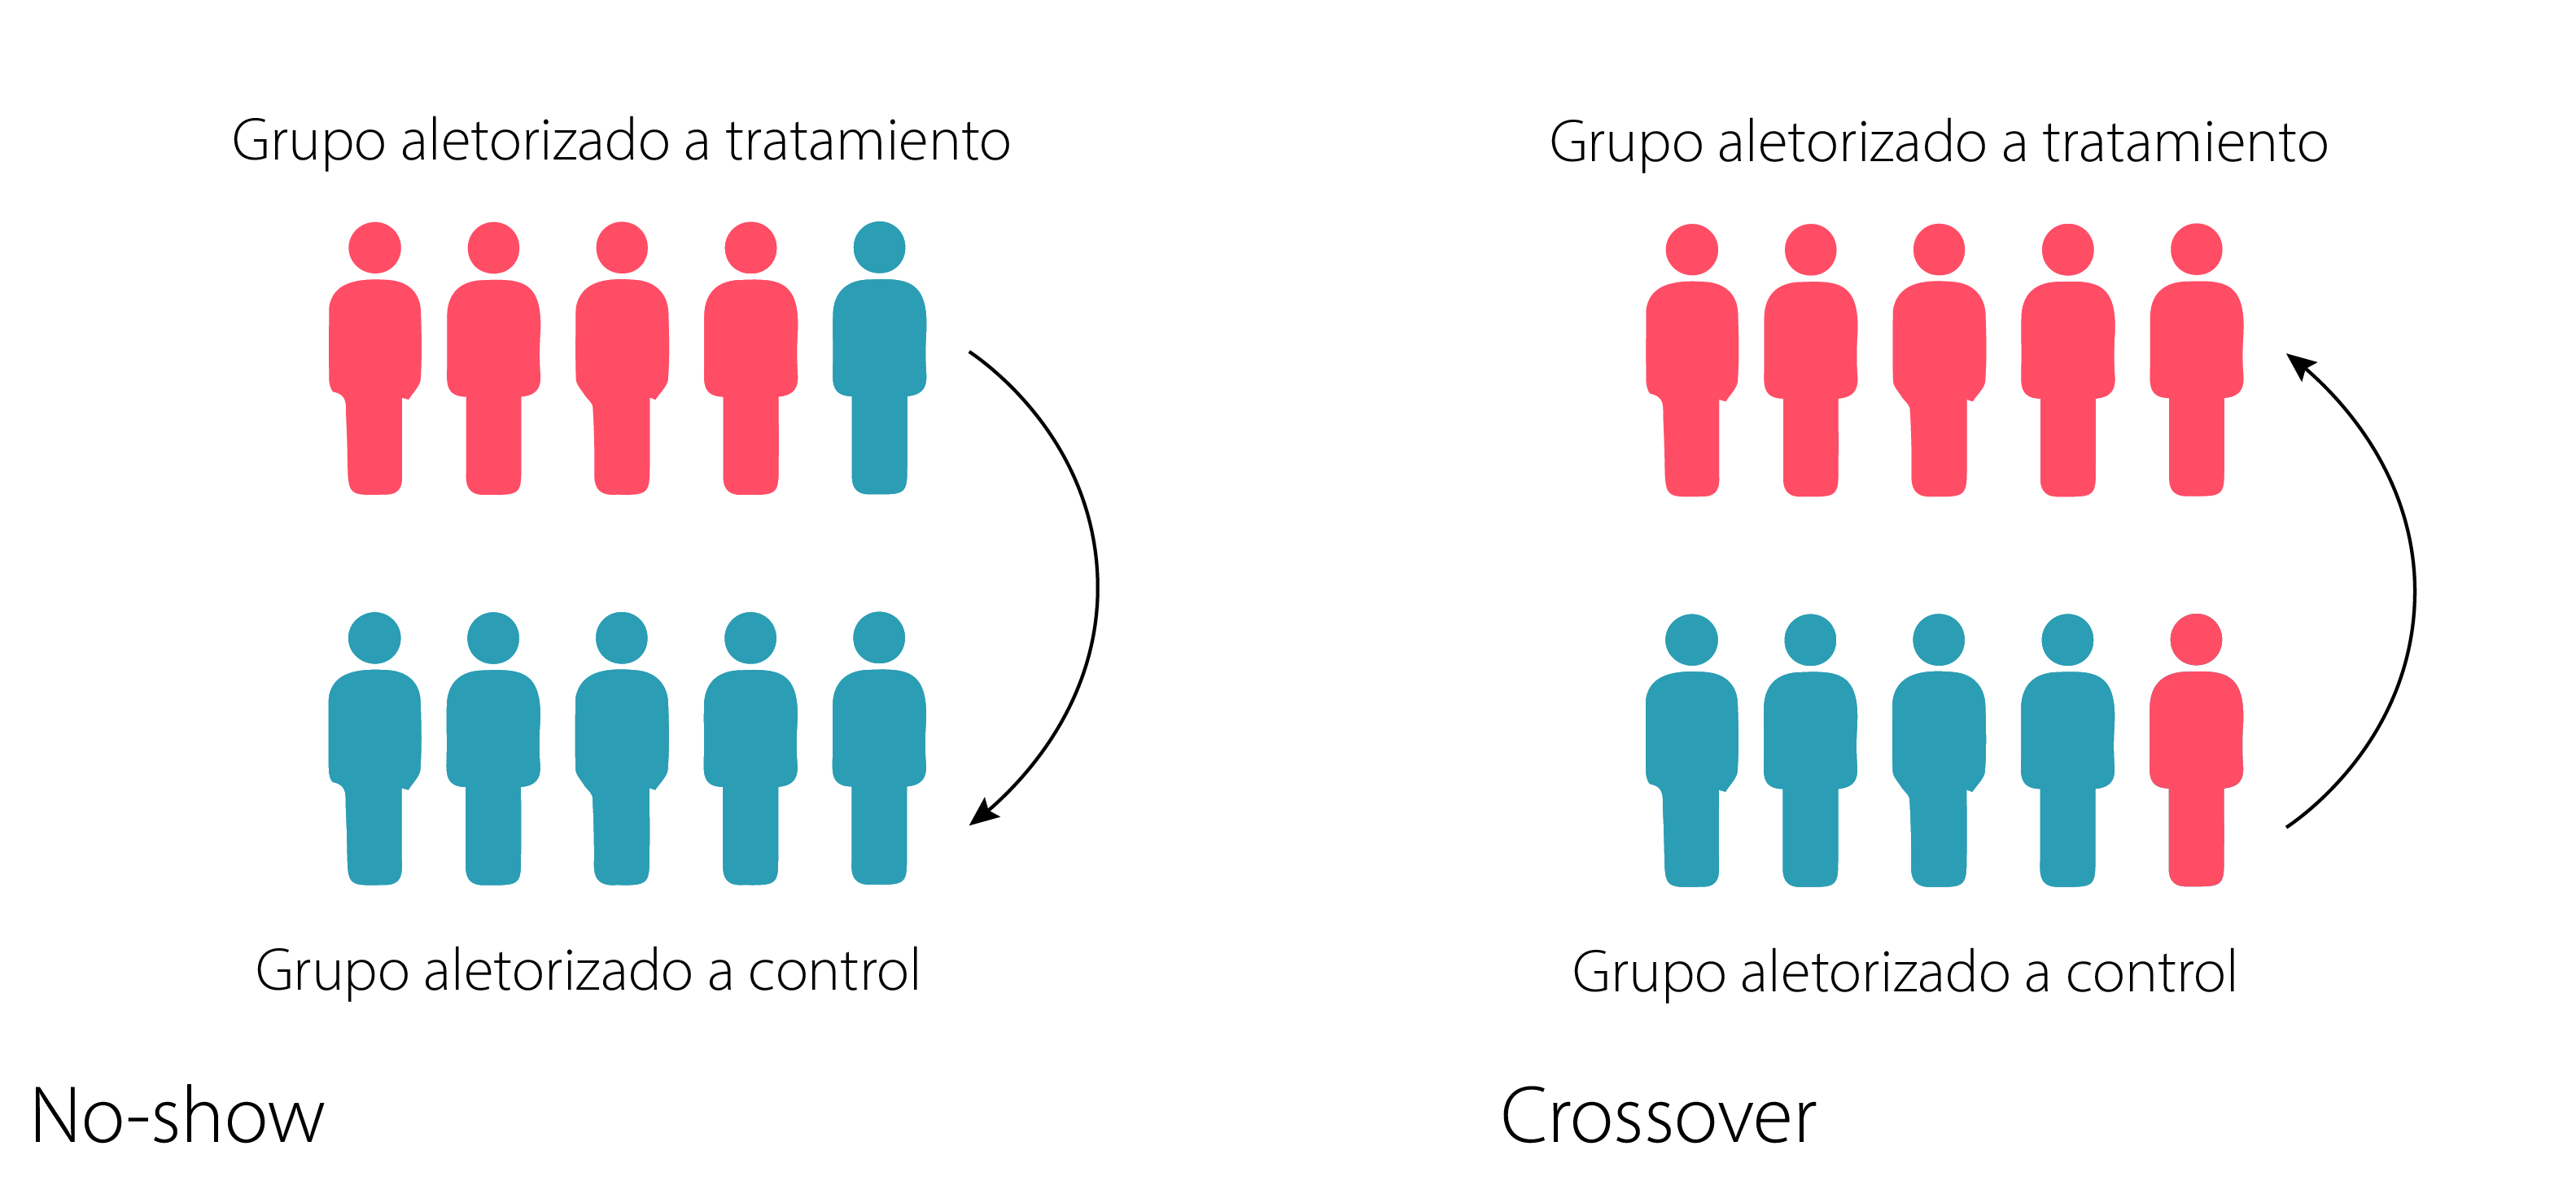
\includegraphics{./imgs/no-adherence-03.jpg}
\end{itemize}

\begin{tcolorbox}[enhanced jigsaw, breakable, rightrule=.15mm, colbacktitle=quarto-callout-warning-color!10!white, bottomtitle=1mm, arc=.35mm, titlerule=0mm, left=2mm, toprule=.15mm, leftrule=.75mm, colback=white, opacitybacktitle=0.6, opacityback=0, colframe=quarto-callout-warning-color-frame, bottomrule=.15mm, coltitle=black, toptitle=1mm, title={Crossovers vs spillovers}]

En este punto es probable que esten confundiendo estos dos términos.
Clarifiquemos. La diferencia puede parecer sutil pero en el
\textbf{spillover} se vulnera la separación entre los grupos, por lo que
la intervención \emph{contamina} sujetos del grupo control pero este
efecto es indirecto (es posible que el sujeto reciba la intervención
parcial, o si la condición de control es otro tratamiento, termine con
recibiendo dos intervenciones -la de su grupo y aquella con la que se
contamino-). En cambio en el \textbf{crossover} hay una reasignación no
intencionada o violación del protocolo, un sujeto asignado al grupo
control, pasa al grupo de tratamiento.

Tratemos de resumir las diferencias en esta tabla:

\begin{longtable}[]{@{}
  >{\raggedright\arraybackslash}p{(\columnwidth - 4\tabcolsep) * \real{0.2500}}
  >{\raggedright\arraybackslash}p{(\columnwidth - 4\tabcolsep) * \real{0.4722}}
  >{\raggedright\arraybackslash}p{(\columnwidth - 4\tabcolsep) * \real{0.2778}}@{}}
\toprule()
\begin{minipage}[b]{\linewidth}\raggedright
\end{minipage} & \begin{minipage}[b]{\linewidth}\raggedright
Crossover
\end{minipage} & \begin{minipage}[b]{\linewidth}\raggedright
Spillover
\end{minipage} \\
\midrule()
\endhead
¿Quién cambia? & El participante recibe otra condición, es el
equivalente a cambiar de grupo & El participante no cambia de grupo \\
¿Qué falla? & La adherencia al grupo asignado & El aislamiento entre
grupos \\
¿Por qué se produce? & Violación del protocolo & Influencias indirectas
entre participantes \\
\bottomrule()
\end{longtable}

\end{tcolorbox}

Como habiamos visto anteriormente los spillovers comprometen la
condicion \textbf{SUTVA} sobre la que se asienta la estimación del
\textbf{ATE} como una diferencia entre los outcomes de ambos grupos. En
este caso la no adherencia compromete la validez interna, ya que puede
sesgar las estimaciones de los efectos del tratamiento. Para mantener la
comparabilidad de los participantes en las condiciones de tratamiento,
lo mejor es tratar de minimizar el incumplimiento de los protocolos de
tratamiento.

Se pueden implementar varias estrategias para impedir que esto ocurra,
por ejemplo:

\begin{itemize}
\item
  Hacer ambos grupos atractivos. La tentación inicial a la hora de
  diseñar un experimento es que el grupo control no reciba absolutamente
  nada. Esto hace que los individuos en el grupo control rápidamente se
  sientan a disgusto ya que esperan algo de beneficio en el participar y
  busquen moverse al grupo tratamiento.
\item
  Tratar de hacer ambos grupos ``fáciles de seguir'' para los
  participantes. En ocasiones el grupo tratamiento tiene que seguir un
  montón de tareas, mientras que el grupo control sólo unas pocas. Este
  escenario hace que muchos sujetos se desanimen en el grupo tratamiento
  y se conviertan en \emph{no-shows}.
\item
  Asegurarse antes de la asignacion que los individuos serán capaces de
  cumplir con cualquiera de las intervenciones. Es importante hacer el
  compromiso explícito con los sujetos que van a completar la
  intervención, no obstante los criterios de exclusión deben diseñarse
  concienzudamente para eliminar a aquellos sujetos que no van a poder
  cumplir con ella. Por ejemplo, es poco probable que un sujeto con un
  trabajo de \(8\) horas diarias pueda cumplir con una intervencion de
  \(6\) horas de caminata diaria.
\end{itemize}

Dijimos que vamos a tratar de evitar la falta de cumplimiento, no
obstante trabajamos con seres humanos y es muy probable que podamos
minimizar este hecho pero vaya a seguir ocurriendo. En estas condiciones
el \textbf{ATE} no puede ser estimado como \textbf{SDO} porque no todos
los sujetos asignados a cada grupo cumplió a rajatabla. Pero no
desesperen que hay alternativas.

\hypertarget{estrategias-para-estimar-el-ate-en-no-cumplimiento}{%
\subsection{Estrategias para estimar el ATE en no
cumplimiento}\label{estrategias-para-estimar-el-ate-en-no-cumplimiento}}

\hypertarget{anuxe1lisis-tratamiento-como-recibido}{%
\subsubsection{\texorpdfstring{Análisis \emph{tratamiento como
recibido}}{Análisis tratamiento como recibido}}\label{anuxe1lisis-tratamiento-como-recibido}}

Pensemos en los escenarios planteados previamente, cuando se dan
\emph{no-shows} y \emph{crossovers} decimos que los sujetos ``se cambian
de grupo'' al recibir o no recibir el tratamiento. Si eso ocurre ¿no
sería lógico analizar a los sujetos de acuerdo al tratamiento recibido
en el grupo que corresponde?

A ver formalicemos un poco el escenario. En los análisis por
\emph{tratamiento recibido}, se conforman dos nuevos grupos: \textbf{a)}
un grupo tratamiento que contiene a los \(D_1 T_1\) (asignados al
tratamiento y que recibieron el tratamiento) y a los \(D_1 T_0\) (los
asignados a la condicion control que recibieron el tratamiento, los
crossover) y \textbf{b)} un grupo control conformado por los \(D_0 T_0\)
y por los \(D_0 T_1\) (los asignados al grupo tratamiento que decidieron
no hacerla o se pasaron al control, es decir los \emph{no-shows})

Parece lógico pero cual es el problema. Bueno el problema radical de
este enfoque es que ocurre \emph{después de la asignación aleatoria},
entonces pueden existir diferencias sistemáticas entre los grupos.

Pensemos esto con un ejemplo. Supongamos que un estudio quiere probar el
efecto de una nueva droga contra el cáncer de pulmón. Al asignar
aleatoriamente a los grupos existen sujetos con distinto grado de
severidad de la enfermedad en ambos grupos. No obstante los sujetos con
mayor severidad del grupo control están muy preocupados por su
enfermedad y deciden buscar el tratamiento por su cuenta (se pasan al
grupo tratamiento), creando una diferencia sistemática. Ahora el grupo
tratamiento tiene sujetos con cuadros clínicos más severos. Sabemos que
los sujetos con cuadros más severos progresan peor, entonces, si el
tratamiento es efectivo, esta análisis tiende a subestimar el efecto de
la droga. También este análisis es suceptible de incluir un sesgo de
causalidad reversa (revisen la sección correspondiente).

\hypertarget{anuxe1lisis-por-protocolo}{%
\subsubsection{\texorpdfstring{Análisis \emph{por
protocolo}}{Análisis por protocolo}}\label{anuxe1lisis-por-protocolo}}

Este análisis es otro enfoque que, aunque puede parecer atractivo a
simple vista, no se recomienda. Este análisis compara
\textbf{únicamente} a quienes completaron los protocolos de tratamiento
tal como les fueron asignados originalmente o sea a los \(D_1 T_1\) (en
el grupo tratamiento) y \(D_0 T_0\) (en el grupo control),los sujetos
\(D_1 T_0\) y los \(D_0 T_1\) son directamente excluídos de todo
análisis.

Este análisis tiene el mismo problema que el enfoque anterior. ¿Por
qué?, porque vuelve a generar diferencias sistemáticas entre los grupos.
Hay que pensar que los sujetos no abandonan uno u otro grupo de forma
aleatoria (como la que generó los grupos) sino por condiciones claves
(muchas veces relacionadas con la misma asignación al grupo) como vimos
en el ejemplo anterior. De esta manera los grupos controles pueden
perder a por ejemplo sujetos con cuadros más severos, porque estos
deciden pasarse a tratamiento, o el grupo tratamiento perder a sujetos
con poca respuesta al tratamiento, porque ante la baja respuesta deciden
abandonar y pasarse al grupo control. De esta forma y dependiendo el
caso este enfoque tiene a subestimar o sobrestimar el efecto. No se
aconseja su uso.

\hypertarget{enfoque-por-intencion-de-tratamiento}{%
\subsection{\texorpdfstring{Enfoque por \textbf{intencion de
tratamiento}}{Enfoque por intencion de tratamiento}}\label{enfoque-por-intencion-de-tratamiento}}

También llamado \emph{intention-to-treat} este enfoque es el que se
prefiere por encima de cualquier otro. En los otros dos vimos que la
asignación o la exclusion de un grupo post-aleatorizacion genera errores
sistemáticos que contaminan la estimación del efecto y pueden abrir una
puerta al sesgo de causalidad reversa. Entonces la mejor solución es
sencillamente no modificar la situación de los sujetos post
aletorización, o sea este enfoque. El lema de este enfoque es
\textbf{analízalos como los aleatorizaste} es decir en el grupo control
se incluyen a todos los sujetos asignados aleatoriamente al grupo
control (\(T_0\)) independiente si recibieron la intervención o no
(cualquier estado de \(D\)) y en el grupo tratamiento todas los \(T_1\)
igualmente.

Cuando hacemos este enfoque, la estimación del efecto cobra otra
realidad y la llamamos estimación de la intención de tratamiento (o
\emph{estimate ITT}) y tiene la siguiente forma:

\[ \text{ITT estimate} = \bar{Y}_T - \bar{Y}_C \ \]

donde \(\bar{Y}_T\) es el resultado medio para el grupo de tratamiento
según fue originalmente asignado, y \(\bar{Y}_C\) es el resultado medio
para el grupo de comparación según fue originalmente asignado.

La estimación \textbf{ITT} tiene la ventaja de comparar participantes
que son \textbf{aleatoriamente equivalentes}. Pero puede ser difícil de
interpretar, dado que es el \emph{efecto promedio de haber ofrecido el
tratamiento en comparación con no haberlo ofrecido}, más que el efecto
promedio del tratamiento si todos hubieran recibido el protocolo de
tratamiento asignado.

Pongamos un ejemplo, se asigna a sujetos a comer salmón tres veces por
semana para bajar el colesterol, esta intervención tiene un efecto real
de reducir el colesterol en un \(20%
\) (este sería el \textbf{ATE} en un mundo ideal). Pero sucede que al
aplicar la intervención la mitad de los sujetos no consumen el salmón (o
sea que son \emph{no-shows}), ellos no tienen un efecto, o sea que
tienen un \(0%
\) de cambio. Si hacemos un análisis de \textbf{ITT}; la \emph{media} de
cambio en los sujetos asignados al grupo tratamiento (\(\bar{Y}_T\) ) es
del \(10%
\) (la mitad cambio un \(20%
\) y la otra mitad \(0%
\)) y la media de cambio del otro grupo (el control,\(\bar{Y}_C\) ) es
\(0%
\) (no incluimos \emph{crossover} en este ejemplo para no complicarnos).
O sea que el estimador \textbf{ITT} es del \(10%
\). El efecto es menor, ¿por qué este enfoque es mejor?

Bueno por un par de razones:

\begin{enumerate}
\def\labelenumi{\arabic{enumi}.}
\item
  \textbf{No hay errores en la direccion de la cadena causal}, nuestro
  objetivo es evaluar como un tratamiento (causa) genera un efecto. Como
  vimos en los enfoques anteriores, al ocurrir un cambio de grupo
  después de la aletorización es frecuente que este cambio esté motivado
  por el efecto mismo de la intervención (una intervención que no
  funciona motiva a que los sujetos se pasen al grupo control, o una
  intervención muy eficaz seduce al grupo control a pasarse a la
  intervención) de esta manera la cadena causal se invierte y es el
  efecto el que genera el tratamiento o no de los sujetos. Al analizar
  los sujetos como fueron asignados no existe una puerta de atrás
  abierta a la reversión de la causalidad.
\item
  \textbf{Puede ser más relevante calcular el ITT que el ATE}, sobretodo
  en políticas públicas o en intervenciones con humanos, el grupo
  investigador (y el grupo que aplicará los resultados) sólo pueden
  llegar al grado de una recomendación, es decir por ejemplo, le dicen a
  un grupo de personas que coman salmón tres veces por semana, no se lo
  meten en la boca. Pensemos en nuestro ejemplo anterior, el gobierno de
  Bolivia quiere iniciar una campaña de concientización de la dieta y
  quiere reducir el colesterol de la población indicándole comer salmón.
  En el país es muy caro el salmón asi que pese a la sugerencia la mitad
  de la población no puede comprarlo, el efecto de esta campaña se
  parecerá más al \textbf{ITT} o al \textbf{ATE}. Exacto, el
  \textbf{ITT} es un mejor estimador de los escenarios del \emph{mundo
  real} (que al fin al cabo es lo qué queremos explicar) porque si una
  intervención es muy buena pero no la pueden recibir todos los sujetos
  a los que se la asignan (por que es muy cara, o porque da efectos
  adversos, o miles de causas más), bueno no es tan buena.
\end{enumerate}

\begin{figure}

{\centering 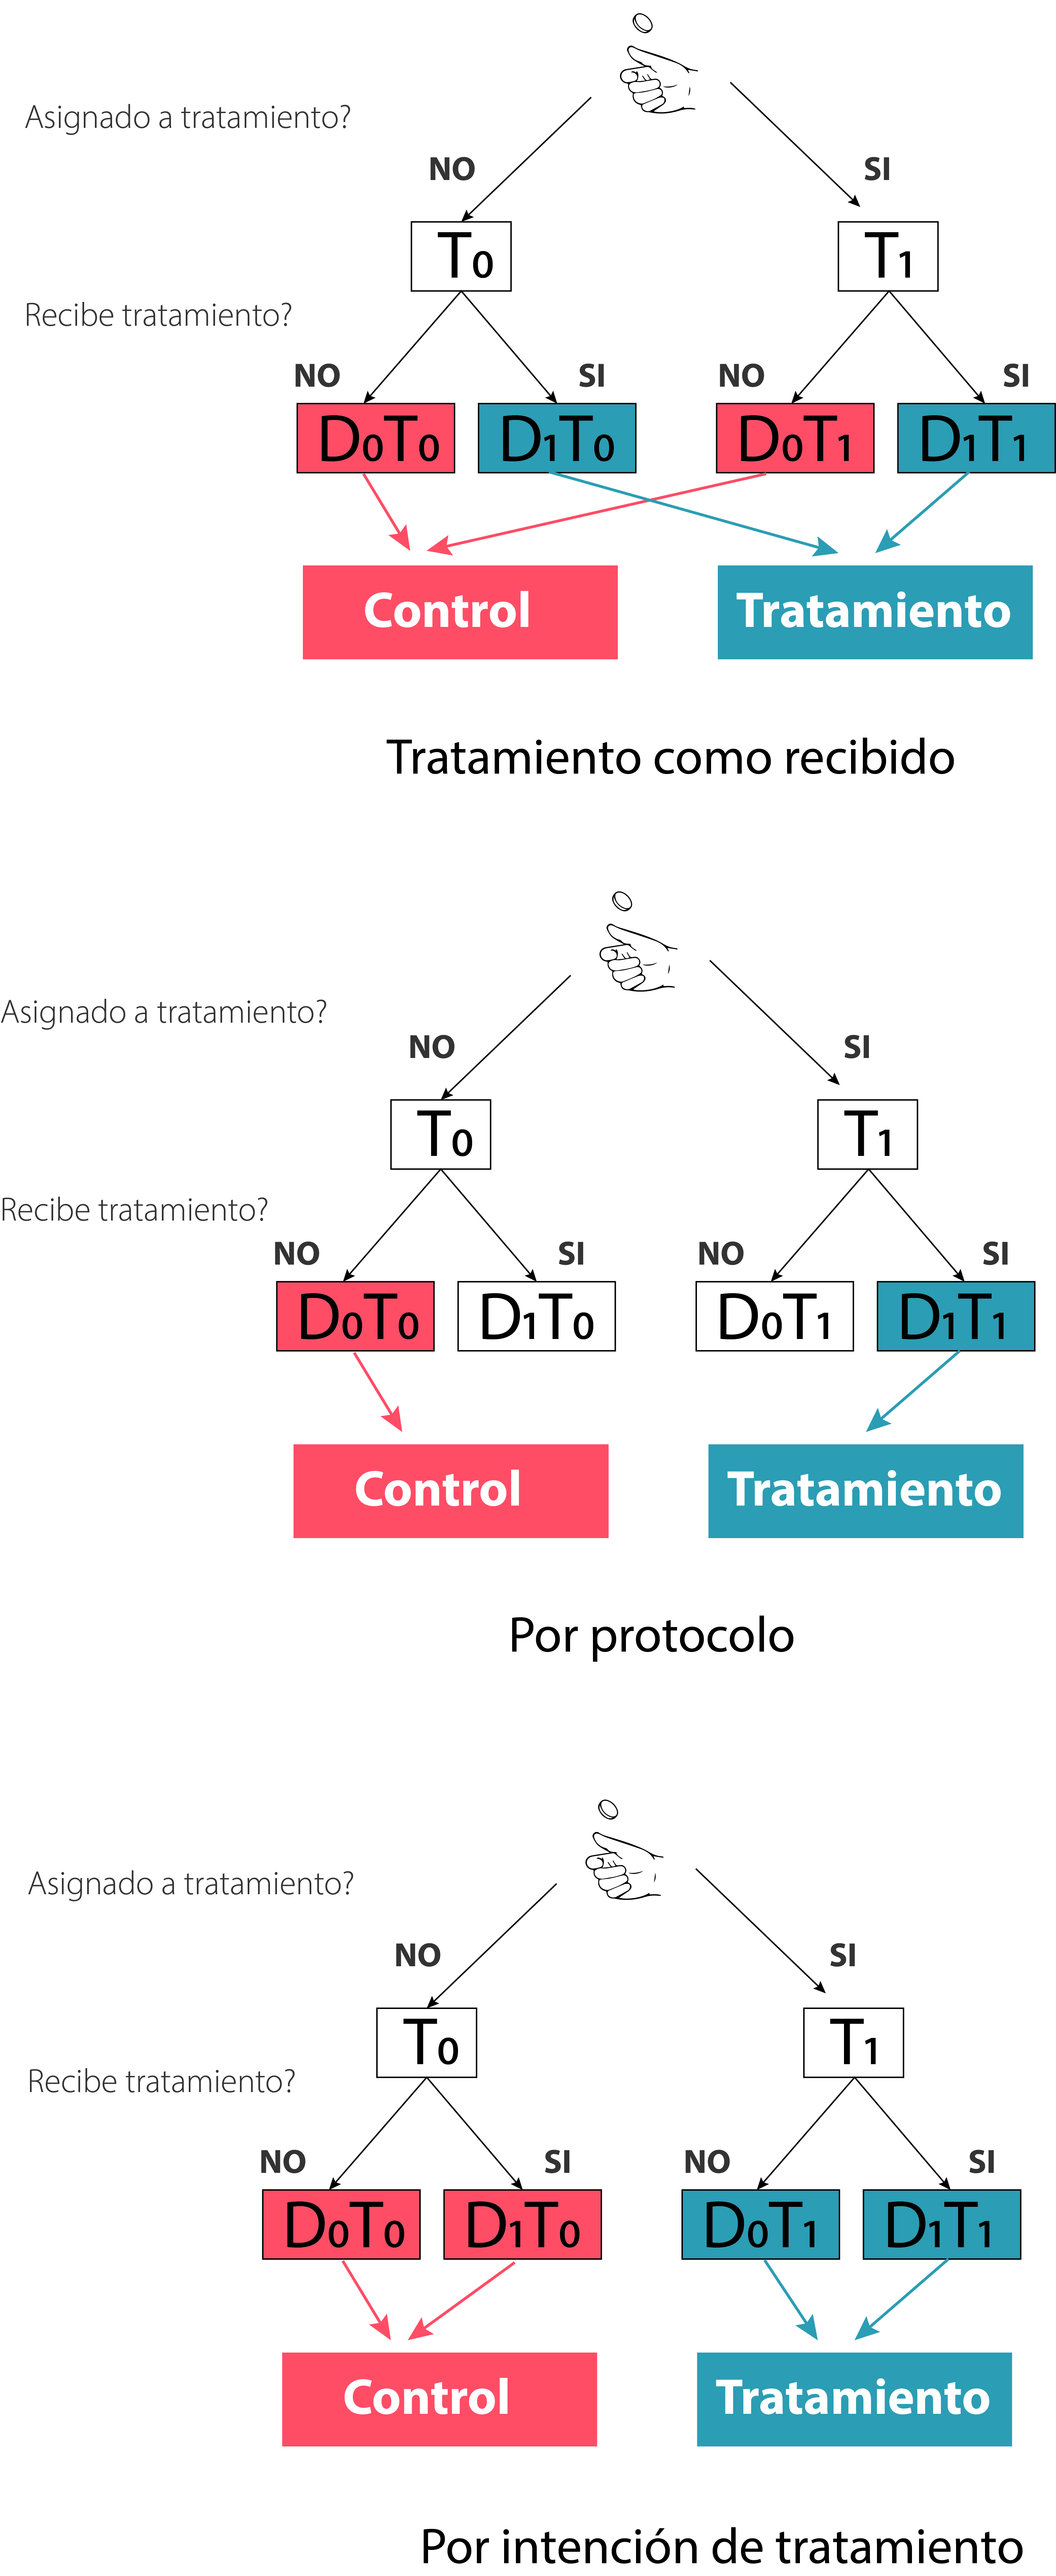
\includegraphics[width=3.125in,height=\textheight]{./imgs/enfoques.jpg}

}

\end{figure}

\bookmarksetup{startatroot}

\hypertarget{cuando-las-asignaciones-no-son-aleatorias}{%
\chapter{\texorpdfstring{\emph{Cuando las asignaciones no son
aleatorias}}{Cuando las asignaciones no son aleatorias}}\label{cuando-las-asignaciones-no-son-aleatorias}}

\hypertarget{el-diseuxf1o-experimental-en-tiempos-de-cuxf3lera}{%
\section{El diseño experimental en tiempos de
cólera\ldots{}}\label{el-diseuxf1o-experimental-en-tiempos-de-cuxf3lera}}

En agosto de 1854 un brote de cólera mataba a una persona cada pocos
minutos en el barrio de Soho, en el centro de Londres. La teoría médica
dominante de la época culpaba a los \emph{miasmas}, una suerte de aire
viciado que se desprendía de la materia en descomposición (spoiler: hoy
sabemos que es una bacteria que proviene de la materia fecal de los
seres humanos y puede contaminar el agua y los alimentos). Mientras el
resto de los médicos de la ciudad se esforzaban en tratar los casos (con
poco éxito), uno de ellos llamado John Snow se propuso atacar el
problema de raíz.Tenía una hipótesis: el cólera se transmitía por el
agua. Para defenderla necesitaba algo más que su intuición. Necesitaba
evidencia.

Snow tomó un mapa de la ciudad y empezó a registrar el domicilio de las
víctimas. Abajo pueden ver una versión moderna en donde el tamaño de las
burbujas representa la cantidad de víctimas en ese punto. La imagen es
contundente, el mapa mostraba claramente que las muertes se concentraban
alrededor de una fuente de agua pública en Broad Street. Efectivamente
el agua de esa bomba estaba contaminada, las autoridades la clausuraron
y la epidemia cesó. Una observación salvó miles de vidas.

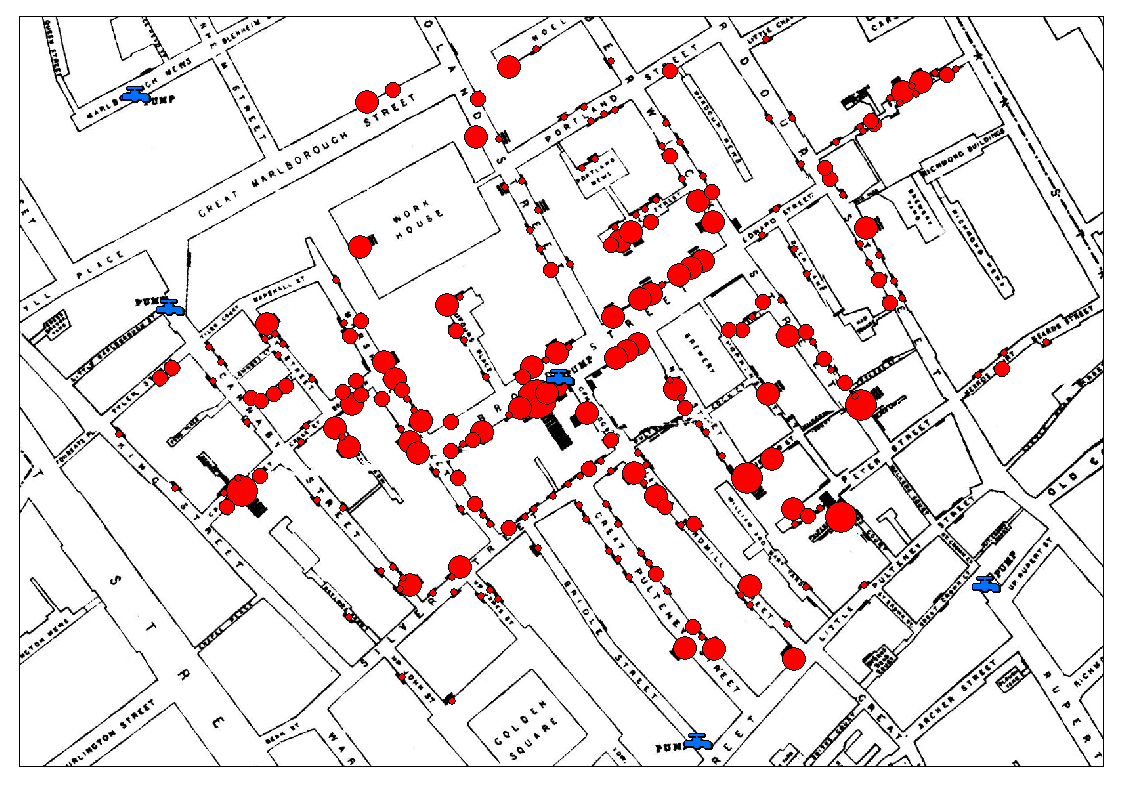
\includegraphics{./imgs/cholera_map.png} Aunque efectiva, ¿alcanzaba la
evidencia de Snow para derrocar la teoría de los miasmas? No.~La
asociación entre la bomba de Broad Street y las muertes podía explicarse
por otras cosas: que el barrio era más pobre, que tenía más
hacinamiento, que compraban alimentos en el mismo mercado o incluso que
compartían la misma intensidad del famoso miasma. Esto es porque pese a
su efectividad, el estudio de Snow era un estudio \textbf{observacional}
y carecen de poder explicativo causal. El lector de este libro se
imaginará que la solución es obvia, Snow necesitaba un
\textbf{experimento aleatorizado} para convencer a sus colegas.Esta
simple solución se da de cabeza contra \emph{``cosillas''} como la
ética, uno no puede andar repartiendo aleatoriamente agua que cree
contaminada con una enfermedad mortal, que la hace imposible.

La cosa no quedó así, en 1855 cuando una nueva epidemia de cólera
estalla (con la bomba de Broad St aún cerrada) Snow advirtió una
situación externa que solucionar el problema de la causalidad. Dos
compañías de agua, \emph{Southwark \& Vauxhall} y \emph{Lambeth},
abastecían las mismas calles del sur de Londres (vean el mapa).

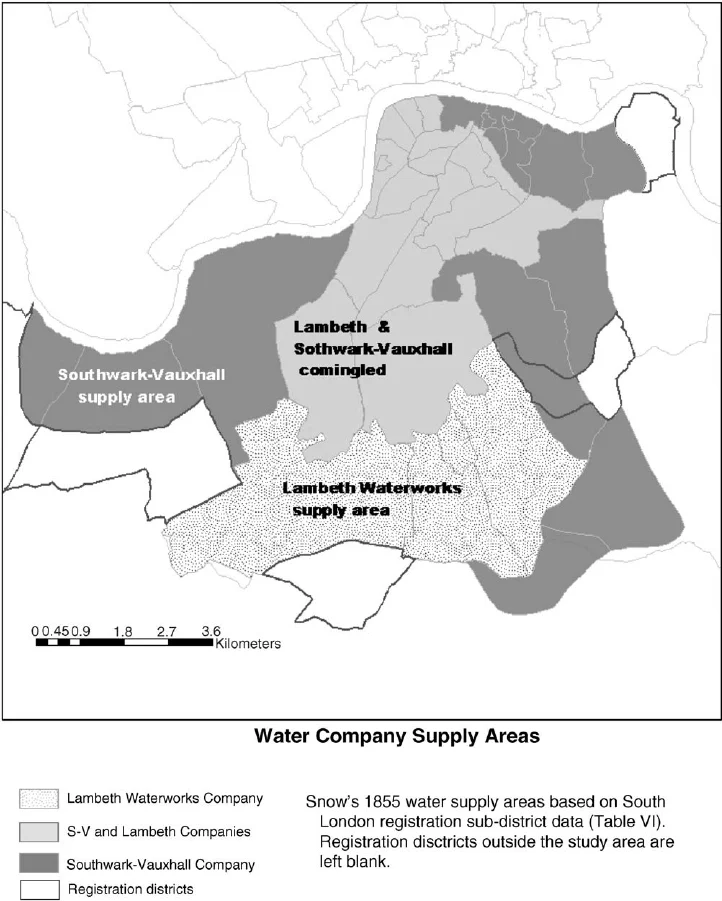
\includegraphics{./imgs/cholera_map_water.png} En 1852, tres años antes
del brote, Lambeth había mudado su toma de agua río arriba, lejos de las
cloacas londinenses. Southwark \& Vauxhall seguía sacando agua del
Támesis contaminado. Casas vecinas, en la misma cuadra, recibían agua de
una u otra compañía según contratos viejos que sus dueños ni recordaban
haber firmado. Los habitantes no podían elegir. Al vivir en el mismo
barrio, e incluso en la misma cuadra, los que bebían agua de una
compañía o la otra eran igual de pobres, con más o menos el mismo
hacinamiento, compraban alimentos en el mismo mercado e incluso
respiraban iguales cantidades del \emph{hipotético} miasma.

Snow contó muertes y armó esta tabla.

\begin{longtable}[]{@{}
  >{\raggedright\arraybackslash}p{(\columnwidth - 6\tabcolsep) * \real{0.2500}}
  >{\raggedright\arraybackslash}p{(\columnwidth - 6\tabcolsep) * \real{0.2500}}
  >{\raggedright\arraybackslash}p{(\columnwidth - 6\tabcolsep) * \real{0.2500}}
  >{\raggedright\arraybackslash}p{(\columnwidth - 6\tabcolsep) * \real{0.2500}}@{}}
\toprule()
\begin{minipage}[b]{\linewidth}\raggedright
Compañía
\end{minipage} & \begin{minipage}[b]{\linewidth}\raggedright
Casas suministradas
\end{minipage} & \begin{minipage}[b]{\linewidth}\raggedright
Muertes por cólera
\end{minipage} & \begin{minipage}[b]{\linewidth}\raggedright
Tasa por 10.000 casas
\end{minipage} \\
\midrule()
\endhead
Southwark \& Vauxhall & 40.046 & 1.263 & 315 \\
Lambeth & 26.107 & 98 & 37 \\
Resto de Londres & 256.423 & 1.422 & 59 \\
\bottomrule()
\end{longtable}

En las casas servidas por Southwark \& Vauxhall murieron 315 personas
por cada 10 000 viviendas. En las servidas por Lambeth, 37. Una
diferencia de casi nueve veces, en barrios idénticos, con el mismo
clima, las mismas casas, las mismas miserias. El único factor que
distinguía sistemáticamente a un grupo del otro era el agua.

Snow no aleatorizó. Pero la naturaleza, las cloacas y los viejos
contratos comerciales habían hecho algo parecido por él.

Este estudio es quizás el primer \textbf{pseudoexperimento} de la
historia, y es de lo que va lo que resta de este libro: \emph{estimar
efectos causales sin asignación aleatoria.}

Este capítulo es la puerta de entrada. Hasta acá venimos hablando de
experimentos donde el investigador asigna los tratamientos por azar y de
ahí se sigue, casi gratis, la posibilidad de identificar efectos
causales. Eso se terminó. A partir de ahora vamos a meternos en el
barro: estudios donde la asignación no es aleatoria, donde el sesgo de
selección no es una posibilidad sino la regla, y donde la identificación
causal hay que defenderla con argumentos, supuestos y diseño.

\hypertarget{la-promesa-que-se-rompe}{%
\section{La promesa que se rompe}\label{la-promesa-que-se-rompe}}

Repasemos brevemente por qué la aleatorización es tan poderosa. En el
capítulo de \emph{potential outcomes} vimos que el problema fundamental
de la inferencia causal es que para cada unidad solo observamos uno de
sus dos resultados potenciales. El otro queda contrafáctico. Y la
diferencia simple de medias entre tratados y no tratados ---el
\textbf{SDO}--- solo es un estimador insesgado del \textbf{ATE} si los
grupos son comparables: si el sesgo de selección y el sesgo de
tratamiento heterogéneo se anulan en esperanza.

La aleatorización resuelve eso de un saque. Cuando asignás el
tratamiento \(D\) por azar, \(D\) se vuelve independiente de los
resultados potenciales:

\[
(Y^0, Y^1) \perp D
\]

Esa independencia garantiza que los dos grupos son intercambiables en
expectativa, y por lo tanto \(E[Y|D=1] - E[Y|D=0]\) estima el
\textbf{ATE} sin trampa. La gracia es que la aleatorización balancea no
solo las variables que medimos, sino también las que no medimos: la
motivación, la severidad subclínica, el contexto familiar, el humor del
día. Por eso es tan barata: no hace falta modelar el mundo.

\begin{tcolorbox}[enhanced jigsaw, breakable, rightrule=.15mm, colbacktitle=quarto-callout-tip-color!10!white, bottomtitle=1mm, arc=.35mm, titlerule=0mm, left=2mm, toprule=.15mm, leftrule=.75mm, colback=white, opacitybacktitle=0.6, opacityback=0, colframe=quarto-callout-tip-color-frame, bottomrule=.15mm, coltitle=black, toptitle=1mm, title=\textcolor{quarto-callout-tip-color}{\faLightbulb}\hspace{0.5em}{Tip}]
Cuando la asignación no es aleatoria, se rompen tres cosas a la vez:

\begin{enumerate}
\def\labelenumi{\arabic{enumi}.}
\tightlist
\item
  \textbf{Los grupos dejan de ser comparables}: tratados y no tratados
  pueden diferir sistemáticamente en cosas que también afectan al
  \emph{outcome}.
\item
  \textbf{Dependemos de supuestos}: ya no alcanza con el diseño; hay que
  defender por qué creemos que la comparación es justa y acordar
  concesiones.
\item
  \textbf{La inferencia estadística depende del modelo}: ya no hay una
  distribución del estimador ``gratis'' garantizada por el sorteo.
\end{enumerate}

Las tres se atacan con distintas herramientas. Este libro las recorre
una por una en los próximos capítulos.
\end{tcolorbox}

La pregunta natural es: ¿por qué no aleatorizamos siempre, entonces?

\hypertarget{por-quuxe9-a-veces-no-se-puede-aleatorizar}{%
\section{¿Por qué a veces no se puede
aleatorizar?}\label{por-quuxe9-a-veces-no-se-puede-aleatorizar}}

Las razones para no aleatorizar son varias, y cada una de ellas motiva
una familia distinta de diseños cuasi-experimentales (o
pseudoexperimentales, son sinónimos).

La razón más obvia es \textbf{ética}. No podés asignar al azar a la
gente a fumar, a sufrir abuso infantil, a divorciarse, a pasar por una
guerra. Cualquier pregunta causal sobre las consecuencias de esas
experiencias está vedada al experimento aleatorizado. Si querés estudiar
el efecto del tabaquismo sobre el cáncer de pulmón, no vas a poder
aleatorizar la exposición. Doll y Hill, en 1950, no aleatorizaron a
nadie a fumar: usaron un estudio de casos y controles, observacional, y
tuvieron que defender su inferencia causal contra las críticas de Fisher
mismo, que sostenía que la asociación entre tabaco y cáncer podía
deberse a confusores no medidos. (White
1990)\marginpar{\begin{footnotesize}\leavevmode\vadjust pre{\protect\hypertarget{ref-white1990}{}}%
White, C. 1990.
{«\href{https://www.ncbi.nlm.nih.gov/pubmed/2192501}{Research on smoking
and lung cancer: a landmark in the history of chronic disease
epidemiology}»}. \emph{Yale Journal of Biology and Medicine} 63 (1):
29-46.\vspace{2mm}\par\end{footnotesize}}

La segunda razón es la \textbf{factibilidad}. No podés aleatorizar
políticas nacionales. El salario mínimo, una reforma migratoria, una ley
de tránsito, un cambio en el sistema previsional: todas son
intervenciones que se aplican a poblaciones enteras, no a individuos.
Tampoco podés aleatorizar terremotos, recesiones o pandemias. La
geografía, el clima y la historia también escapan del control del
investigador.

Una tercera razón es la \textbf{retrospectividad}. Muchas veces la
pregunta surge después de que el ``tratamiento'' ya ocurrió. ¿La
pandemia de 2020 aumentó la prevalencia de depresión? La pandemia ya
pasó. No hay forma de aleatorizar el COVID \emph{post hoc}.

A las que ya nombramos se suman dos más, un poco menos dramáticas pero
igual de habituales. El \textbf{costo y la escala} vuelven prohibitivos
algunos experimentos que en teoría serían posibles: muestras enormes,
seguimientos de treinta años, múltiples países simultáneamente. Y el
\textbf{cumplimiento}: aun cuando lograste aleatorizar, los
participantes eligen. El asignado a tratamiento puede no recibirlo, el
asignado a control puede conseguirlo por afuera. El estimador
\emph{intention-to-treat} sigue siendo causal, pero deja sin contestar
la pregunta clínica de fondo, que es qué le pasa al que efectivamente
recibe el tratamiento.

Una última razón, más sutil, es la \textbf{validez externa}. Un ensayo
aleatorizado puede funcionar perfecto en un hospital terciario con
voluntarios sanos y bien adheridos, y no decir nada útil sobre la
población real, donde los pacientes son más viejos, tienen
comorbilidades y abandonan los tratamientos por la mitad. A veces el
cuasi-experimento, paradójicamente, gana en validez externa lo que
pierde en validez interna respecto al \textbf{RCT}.

\hypertarget{quuxe9-es-un-cuasi-experimento-entonces}{%
\section{¿Qué es un cuasi-experimento
entonces?}\label{quuxe9-es-un-cuasi-experimento-entonces}}

Acá conviene poner palabras precisas.

\begin{tcolorbox}[enhanced jigsaw, breakable, colback=white, rightrule=.15mm, opacityback=0, colframe=quarto-callout-color-frame, bottomrule=.15mm, left=2mm, toprule=.15mm, leftrule=.75mm, arc=.35mm]
Un \textbf{cuasi-experimento} (o pseudoexperimento, dependiendo del
autor que leas) es un estudio que busca estimar el efecto causal de un
tratamiento sin asignación aleatoria, pero recurriendo a otros recursos
(de diseño y de análisis) para aproximar la comparabilidad que el
experimento aleatorizado produciría por construcción.
\end{tcolorbox}

La frase importante de esa definición es \emph{``otros recursos de
diseño y análisis''}. Un cuasi-experimento no es un estudio
observacional al que después le pegamos una regresión cualquiera. Es un
diseño en el que pensamos activamente, antes de mirar los datos, cómo
elegir el grupo de comparación, qué variación explotar, qué momento
aprovechar. La inferencia causal en un cuasi-experimento se defiende con
el diseño primero y con el modelo después.

Es útil distinguir tres tipos de estudio que a veces se confunden:

\begin{tcolorbox}[enhanced jigsaw, breakable, rightrule=.15mm, colbacktitle=quarto-callout-tip-color!10!white, bottomtitle=1mm, arc=.35mm, titlerule=0mm, left=2mm, toprule=.15mm, leftrule=.75mm, colback=white, opacitybacktitle=0.6, opacityback=0, colframe=quarto-callout-tip-color-frame, bottomrule=.15mm, coltitle=black, toptitle=1mm, title=\textcolor{quarto-callout-tip-color}{\faLightbulb}\hspace{0.5em}{Tip}]

\begin{itemize}
\item
  \textbf{Experimento aleatorizado}: el investigador controla la
  asignación al tratamiento y la aleatoriza. La identificación causal
  sale del diseño. La amenaza principal es el cumplimiento y la validez
  externa.
\item
  \textbf{Cuasi-experimento}: hay una intervención y un grupo de
  comparación, pero la asignación no es aleatoria. La identificación
  causal sale del diseño \emph{más} supuestos. La amenaza principal es
  la selección sobre variables no observadas.
\item
  \textbf{Estudio observacional puro}: ni siquiera hay una intervención
  clara; la ``exposición'' surge de la vida misma. La identificación
  causal depende casi enteramente de supuestos. Las amenazas son la
  confusión y la selección por todos lados.
\end{itemize}

Las tres familias pueden usar datos parecidos. Lo que las distingue no
es el tipo de dato, es de dónde sale la identificación.

\end{tcolorbox}

Cuando lean un paper, esta clasificación les sirve para diagnosticar de
entrada qué nivel de evidencia están viendo. Un ensayo aleatorizado bien
hecho descansa sobre el diseño. Un estudio retrospectivo con regresión
múltiple descansa, casi enteramente, sobre la fe en que los confusores
fueron medidos.

\hypertarget{las-cuatro-validez}{%
\section{Las cuatro validez}\label{las-cuatro-validez}}

Al hablar de las diferencias entre diseños introdujimos casualmente los
términos de validez y amenaza a esta. Pero, ¿de que se trata? Shadish,
Cook y Campbell usaron el término \textbf{validez} para denotar en qué
medida una inferencia (sobre un efecto, una medición o una
generalización) es correcta (Shadish, Cook, y Campbell
2002)\marginpar{\begin{footnotesize}\leavevmode\vadjust pre{\protect\hypertarget{ref-shadish2002}{}}%
Shadish, William R., Thomas D. Cook, y Donald T. Campbell. 2002.
\emph{Experimental and Quasi-Experimental Designs for Generalized Causal
Inference}. Boston, MA: Houghton Mifflin.\vspace{2mm}\par\end{footnotesize}}.
Estos autores reconocen entonces que hay ciertos niveles de esa
``corrección''. No hay una sola validez sino cuatro variedades clásicas.
Las cuatro hacen preguntas distintas sobre el mismo estudio, y un
trabajo serio tiene que defenderse en las cuatro.

\hypertarget{validez-estaduxedstica}{%
\subsection{Validez estadística}\label{validez-estaduxedstica}}

La \textbf{validez estadística} pregunta si la covariación que
observamos es real o si es ruido. ¿Tenés potencia suficiente para
detectar el efecto que esperás? ¿Estás corrigiendo por comparaciones
múltiples? ¿La distribución de los datos cumple con los supuestos del
test que elegiste? ¿Estás reportando todos los análisis que corriste o
solo los que dieron bien?

La neurociencia cognitiva vivió una crisis pública en torno a esto.
Bennett y colegas (Bennett et~al.
2011)\marginpar{\begin{footnotesize}\leavevmode\vadjust pre{\protect\hypertarget{ref-bennett2011}{}}%
Bennett, Craig M., Abigail A. Baird, Michael B. Miller, y George L.
Wolford. 2011. {«Neural Correlates of Interspecies Perspective Taking in
the Post-Mortem Atlantic Salmon: An Argument For Multiple Comparisons
Correction»}. \emph{Journal of Serendipitous and Unexpected Results} 1
(1): 1-5.\vspace{2mm}\par\end{footnotesize}},
en 2009, le hicieron una resonancia magnética funcional a un salmón
muerto mientras le mostraban fotos de personas con distintas emociones.
Sin corrección por comparaciones múltiples, encontraron ``activación''
significativa en el cerebro del pez. El punto era didáctico: con 130.000
vóxeles y un umbral de significancia de \(p<0{,}001\), los falsos
positivos son matemáticamente inevitables. Una conclusión causal apoyada
en validez estadística mala no es causal: es un artefacto.

\hypertarget{validez-interna}{%
\subsection{Validez interna}\label{validez-interna}}

La \textbf{validez interna} pregunta si esa covariación, dado que es
real, es causal. ¿Hay un mecanismo confiable que vaya del tratamiento al
\emph{outcome}, o lo que veo podría explicarse por otra cosa? Es el
corazón del libro y se la juega contra la lista de amenazas que vemos en
la sección siguiente.

Pensá en los estudios pre-post de estimulación magnética transcraneal en
depresión resistente sin grupo control: muestran mejorías reales,
claramente significativas. Pero la depresión también mejora sola con el
tiempo, los pacientes consultan en el pico del episodio y regresan a la
media, y la expectativa del tratamiento activo se suma al efecto. La
covariación es real; la inferencia causal, en cambio, está armada con
palitos.

\hypertarget{validez-de-constructo}{%
\subsection{Validez de constructo}\label{validez-de-constructo}}

La \textbf{validez de constructo} pregunta si lo que medimos representa
el constructo teórico que dijimos estar midiendo. Es la más fácil de
pasar por alto, porque vive en el límite entre la psicometría y la
teoría.

En neurociencia cognitiva el problema es endémico. ``Memoria de
trabajo'' medida con por ejemplo un test \emph{n-back} de dos no es lo
mismo que medida con span de dígitos: las dos tareas correlacionan
modestamente y reclutan circuitos parcialmente distintos en el cerebro.
Si tu estudio dice ``el tratamiento mejora la memoria de trabajo'' y
solo medís \emph{n-back}, estás haciendo una afirmación más amplia que
la que sostienen tus datos. Pasa lo mismo con ``atención'': test como
Stroop, CPT y búsqueda visual miden cosas emparentadas pero no
idénticas. En economía vale el paralelo con el desempleo: si el
indicador oficial no incluye a los desalentados que dejaron de buscar
trabajo, lo que medís deja afuera justo el margen donde más cambian las
cosas. La validez de constructo no es un problema de medición sucia: es
un problema de definir qué estás midiendo.

\hypertarget{validez-externa}{%
\subsection{Validez externa}\label{validez-externa}}

La \textbf{validez externa} pregunta si lo que encontramos generaliza a
otras personas, otros lugares, otros tiempos, otras dosis. En
neurociencia cognitiva la pregunta clásica es si una tarea de
laboratorio ---con el sujeto inmóvil dentro de un resonador o frente a
una pantalla en una habitación oscura--- mide algo que se parezca al uso
de la atención, la memoria o el control inhibitorio en la vida
cotidiana. La crítica de Henrich, Heine y Norenzayan sobre las muestras
\emph{WEIRD} (occidentales, educadas, industrializadas, ricas y
democráticas) golpea acá: si la evidencia que sostiene una afirmación
general se generó con estudiantes universitarios norteamericanos, la
generalización a otras poblaciones está sin testear.

En economía experimental la versión equivalente es la del laboratorio.
Los participantes ---estudiantes, otra vez--- juegan con sumas pequeñas,
en una computadora, sabiendo que están en un experimento. Las
preferencias por el riesgo, la cooperación o la honestidad medidas ahí a
veces predicen bien el comportamiento real y a veces no. Cuando no lo
hacen, no es que el experimento estaba mal: es que la generalización
requiere supuestos que conviene explicitar.

\hypertarget{jerarquuxeda-de-la-validez}{%
\subsection{Jerarquía de la validez}\label{jerarquuxeda-de-la-validez}}

Si bien las cuatro importan, hay una jerarquía operativa. En cualquier
diseño es lógico pensar en este orden: Primero si la covariación es real
(validez estadística), después, si esta señal es causal (validez
interna), después si esto que dije que era realmente lo es (validez de
constructo), y recién al final se discute si generaliza (validez
externa). Si se falló en alguno de los tres primeros, la discusión sobre
validez externa es prematura.

La validez interna es el principal desafío del diseño experimental. La
razón está bien resumida en una frase de Reichardt: si la covariación
que observamos no es causal, generalizar no-causalidad a otros contextos
no tiene sentido. Si fallamos en identificar el efecto causal
\emph{acá}, no nos interesa demasiado si ``generalizaría'' a otra
población. Estaríamos generalizando un artefacto. Esto no quiere decir
que la validez externa no importe, importa muchísimo en políticas
públicas y en clínica, sino que hay un orden.

\hypertarget{amenazas-a-la-validez-interna}{%
\section{Amenazas a la validez
interna}\label{amenazas-a-la-validez-interna}}

Si es tan importante, la cuestión operativa que sigue es: ¿cómo se
evalúa la validez interna? La respuesta breve es que no hay un test. Hay
una lista de \textbf{amenazas}, cada una con su lógica, y para cada
amenaza hay defensas específicas.

Vamos a las más frecuentes.

\hypertarget{historia-y-maduraciuxf3n}{%
\subsection{Historia y maduración}\label{historia-y-maduraciuxf3n}}

Son las dos amenazas más básicas y, por lo mismo, las más subestimadas.
La \textbf{historia} es cualquier evento externo al tratamiento que
ocurre entre la medición pre y post. Por ejemplo, si estás midiendo el
efecto de un programa de intervención sobre depresión, y a mitad del
seguimiento entra una cuarentena nacional. ¿El cambio observado se debe
al programa o a la cuarentena? Sin grupo control, no podés separarlos.

La \textbf{maduración} es más sutil. Los participantes cambian con el
tiempo sin que nadie haga nada. Un niño con trastorno del lenguaje
mejora con seis meses de fonoaudiología, pero también mejora con seis
meses sin fonoaudiología, porque maduró. Si comparás antes y después en
el grupo tratado y no tenés un grupo control que envejezca al mismo
ritmo, no podés separar el efecto del tratamiento de la trayectoria del
desarrollo.

Las dos amenazas tienen la misma cura: un grupo de comparación expuesto
a la historia y a la maduración pero no al tratamiento. Esa es, no por
casualidad, la lógica de varios de los métodos que vienen.

\hypertarget{testing-e-instrumentaciuxf3n}{%
\subsection{Testing e
instrumentación}\label{testing-e-instrumentaciuxf3n}}

El efecto de \textbf{testing} aparece cuando tomar un test cambia el
resultado de la siguiente toma. Un ejemplo clásico, en cualquier
evaluación cognitiva hay test con efecto de aprendizaje (sobretodo en
los test de memoria), entonces el participante mejora la segunda vez
simplemente porque ya conoce el formato. Si comparás pre-post sin grupo
control, no estás midiendo recuperación cognitiva; estás midiendo cuánto
se aprende a hacer el test.

La \textbf{instrumentación} es el problema espejo: lo que cambia no es
el sujeto sino el instrumento o quien lo aplica. En la medición
\emph{pre} evalúa, por ejemplo, un residente de primer año, al llegar al
tiempo \emph{post} el evaluador ya es un el médico de planta y su
evaluación es más estricta. También puede ocurrir que cambia el aparato,
o el formulario u otro elemento de captura de los datos. Cualquier
cambio en \emph{cómo} medimos puede confundirse con un cambio real.

\hypertarget{regresiuxf3n-a-la-media}{%
\subsection{Regresión a la media}\label{regresiuxf3n-a-la-media}}

Esta es probablemente la amenaza más sutil y la más frecuentemente
ignorada. Cuando seleccionás a los participantes por valores extremos,
las mediciones siguientes tienden a estar más cerca de la media,
\emph{aun sin intervención}. Es estadística pura: si una observación es
muy alta, una parte de esa altura es señal y otra parte es ruido. El
ruido no se repite, así que la siguiente medición, si los sujetos no
recibieron nada, tiende a ser un poco más baja.

La regresión a la media engaña muy bien. Si reclutás al 10\% más
deprimido de una población clínica y los seguís en el tiempo, sus
puntajes promedio van a bajar de \emph{tiempo 0} a \emph{tiempo 1}, de
\emph{tiempo 1} a \emph{tiempo 2}. Si en el medio les diste un
tratamiento, no podés saber qué parte de la mejora se debe al mismo (a
lo mejor absolutamente nada) y qué parte es regresión a la media.

Veamos esto con un ejemplo simulado. Generamos 1000 personas con un
puntaje base (un constructo estable, digamos un \emph{score de
depresión} donde más alto es peor) y una medición ruidosa de ese
constructo en dos momentos. Después seleccionamos al 10\% con
\emph{peor} medición en t0 ---los más deprimidos--- y vemos qué les pasa
en t1, sin intervención de ningún tipo.

\begin{Shaded}
\begin{Highlighting}[]
\FunctionTok{library}\NormalTok{(tidyverse)}
\FunctionTok{set.seed}\NormalTok{(}\DecValTok{42}\NormalTok{)}

\CommentTok{\# 1000 personas con un rasgo estable + ruido en dos mediciones}
\NormalTok{n }\OtherTok{\textless{}{-}} \DecValTok{1000}
\NormalTok{datos }\OtherTok{\textless{}{-}} \FunctionTok{tibble}\NormalTok{(}
  \AttributeTok{id =} \DecValTok{1}\SpecialCharTok{:}\NormalTok{n,}
  \AttributeTok{rasgo =} \FunctionTok{rnorm}\NormalTok{(n, }\AttributeTok{mean =} \DecValTok{0}\NormalTok{, }\AttributeTok{sd =} \DecValTok{1}\NormalTok{),}
  \AttributeTok{y\_t0  =}\NormalTok{ rasgo }\SpecialCharTok{+} \FunctionTok{rnorm}\NormalTok{(n, }\AttributeTok{mean =} \DecValTok{0}\NormalTok{, }\AttributeTok{sd =} \DecValTok{1}\NormalTok{),}
  \AttributeTok{y\_t1  =}\NormalTok{ rasgo }\SpecialCharTok{+} \FunctionTok{rnorm}\NormalTok{(n, }\AttributeTok{mean =} \DecValTok{0}\NormalTok{, }\AttributeTok{sd =} \DecValTok{1}\NormalTok{)}
\NormalTok{)}

\CommentTok{\# Seleccionamos al 10\% con peor puntaje (mayor) en t0}
\NormalTok{umbral }\OtherTok{\textless{}{-}} \FunctionTok{quantile}\NormalTok{(datos}\SpecialCharTok{$}\NormalTok{y\_t0, }\FloatTok{0.90}\NormalTok{)}
\NormalTok{seleccion }\OtherTok{\textless{}{-}}\NormalTok{ datos }\SpecialCharTok{\%\textgreater{}\%} \FunctionTok{filter}\NormalTok{(y\_t0 }\SpecialCharTok{\textgreater{}=}\NormalTok{ umbral)}

\CommentTok{\# Comparamos promedios pre y post en el grupo seleccionado}
\NormalTok{seleccion }\SpecialCharTok{\%\textgreater{}\%}
  \FunctionTok{summarise}\NormalTok{(}\AttributeTok{media\_t0 =} \FunctionTok{mean}\NormalTok{(y\_t0),}
            \AttributeTok{media\_t1 =} \FunctionTok{mean}\NormalTok{(y\_t1),}
            \AttributeTok{mejora   =}\NormalTok{ media\_t0 }\SpecialCharTok{{-}}\NormalTok{ media\_t1)}
\CommentTok{\#\textgreater{} \# A tibble: 1 x 3}
\CommentTok{\#\textgreater{}   media\_t0 media\_t1 mejora}
\CommentTok{\#\textgreater{}      \textless{}dbl\textgreater{}    \textless{}dbl\textgreater{}  \textless{}dbl\textgreater{}}
\CommentTok{\#\textgreater{} 1     2.44     1.25   1.19}
\end{Highlighting}
\end{Shaded}

El grupo seleccionado ``mejora'' entre t0 y t1, su puntaje baja en
promedio más de un punto, aunque no hicimos nada. La diferencia viene de
la regresión a la media: en t0 fueron seleccionados por valores altos, y
parte de esos valores altos era ruido que no se repitió.

En efecto, si un estudio recluta a pacientes severos y los miden
pre-post sin grupo control concurrente, vas a ver una mejoría aún si el
tratamiento es agua tibia. Necesitan un control seleccionado con el
mismo criterio para descontar este efecto.

\hypertarget{sesgo-de-selecciuxf3n-y-no-adherencia}{%
\subsection{Sesgo de selección y
no-adherencia}\label{sesgo-de-selecciuxf3n-y-no-adherencia}}

Llegamos al corazón del problema en los cuasi-experimentos. El
\textbf{sesgo de selección} es el grado en que difieren sistemáticamente
los individuos que terminan siendo tratados de quienes no, en cosas que
también afectan el \emph{outcome}. Por ejemplo, si el criterio de
asignacion a un tratamiento como la cirugía bariátrica (una cirugía para
adelgazar) es la preferencia de los pacientes. Puede ocurrir que los
pacientes que eligen una cirugía bariátrica difieran del grupo placebo
porque están más motivados, tienen mejor adherencia, mejor red social y
probablemente mejor estatus socioeconómico. Si comparás sus desenlaces
con los de quienes no se operaron, estás mezclando el efecto de la
cirugía con el efecto de todo lo demás que distingue a los dos grupos.

Acuerdense que lo formalizamos en el capítulo de potential outcomes de
la siguiente forma.

\begin{equation}\protect\hypertarget{eq-selection_bias}{}{
\begin{array}
\underbrace{E[Y_i^0|D_i=1] - E[Y_i^0|D_i=0] }
\end{array}
}\label{eq-selection_bias}\end{equation}

En el capítulo anterior lo presentamos como un término en una
descomposición algebraica. Acá lo presentamos como una pregunta de
investigación: ¿quiénes eligieron meterse en el grupo tratado, y por
qué? La respuesta, casi siempre, es que eligieron por razones que no son
ajenas al \emph{outcome}.

Otra amenaza ya conocida es la \textbf{no adherencia}. Vista en este
marco, la no-adherencia funciona como un sesgo de selección
post-aleatorización (o post-asignación del tratamiento). La razón por la
que funciona similar al sesgo de selección es que los que abandonan no
son aleatorios, frecuentemente lo hacen por razones sistemáticas ligadas
al outcome. Esto último crea diferencias sistemáticas en los grupos que
persisten en el tratamiento asignado.

\begin{tcolorbox}[enhanced jigsaw, breakable, colback=white, rightrule=.15mm, opacityback=0, colframe=quarto-callout-color-frame, bottomrule=.15mm, left=2mm, toprule=.15mm, leftrule=.75mm, arc=.35mm]
Casi todos los métodos que vas a ver en los próximos capítulos
---matching, variables instrumentales, diferencias en diferencias,
regresión discontinua--- son, en el fondo, estrategias distintas para
atacar el problema de selección.
\end{tcolorbox}

\hypertarget{difusiuxf3n-compensaciuxf3n-y-otros-fenuxf3menos-sociales}{%
\subsection{Difusión, compensación y otros fenómenos
sociales}\label{difusiuxf3n-compensaciuxf3n-y-otros-fenuxf3menos-sociales}}

Algunas amenazas son específicas de las evaluaciones de programas y de
las intervenciones en contextos sociales o institucionales. Estas ya las
vimos brevemente en el capítulo de \emph{potential outcomes} como
violaciones del \textbf{SUTVA}, pero conviene tenerlas presentes acá
también, porque aparecen todo el tiempo en cuasi-experimentos.

La \textbf{difusión} o \textbf{spillover} ocurre cuando el grupo control
adopta partes del tratamiento. En un ensayo comunitario de prevención,
una campaña de información puede ``contagiar'' al barrio control. La
\textbf{rivalidad compensatoria} es el caso en que el grupo control, al
saberse desventajado, se esfuerza más para no quedar atrás, lo que
reduce la diferencia observada. La \textbf{desmoralización resentida} es
el opuesto: los del control se desmotivan al percibirse injustamente
tratados, y la diferencia con los tratados se infla artificialmente.

Estas amenazas no son exóticas. En cualquier intervención escolar,
hospitalaria o comunitaria donde los grupos están en contacto y se
enteran de su asignación, alguna de las tres está probablemente
operando.

\hypertarget{no-todo-es-color-de-rosa-la-advertencia-de-lalonde}{%
\section{No todo es color de rosa: la advertencia de
Lalonde}\label{no-todo-es-color-de-rosa-la-advertencia-de-lalonde}}

Si Snow nos inspira con la posibilidad de hacer causalidad sin
laboratorio, Robert Lalonde, (LaLonde
1986)\marginpar{\begin{footnotesize}\leavevmode\vadjust pre{\protect\hypertarget{ref-lalonde1986}{}}%
LaLonde, Robert J. 1986. {«Evaluating the Econometric Evaluations of
Training Programs with Experimental Data»}. \emph{The American Economic
Review} 76 (4): 604-20. \url{https://www.jstor.org/stable/1806062}.\vspace{2mm}\par\end{footnotesize}}
en 1986, nos advierte cuán fácil es engañarse en el camino.

Lalonde realizó la siguiente demostración. Utilizó datos de un programa
de empleo asistido en Estados Unidos, el \emph{National Supported Work
Demonstration}, que había sido evaluado mediante un experimento
aleatorizado. La pregunta que planteó fue contrafáctica y elegante: si
no hubiéramos contado con el experimento con asignación aleatoria y el
programa simplemente se hubiera implementado, la única alternativa para
estimar su efecto habría sido comparar a los participantes del programa
con un grupo de control construido a partir de encuestas nacionales en
las que el programa no se había aplicado. En esas condiciones,
¿habríamos llegado al mismo resultado?

La respuesta corta es que no. El experimento aleatorio estimaba un
aumento promedio de unos 886 dólares en los ingresos anuales de los
participantes. Las comparaciones contra controles observacionales,
ajustadas con las técnicas habituales de regresión, daban estimaciones
que variaban en miles de dólares y a veces tenían el signo contrario. Es
decir: si hubieras hecho el estudio con datos observacionales y los
hubieras analizado con buena fe, habrías concluido que el programa
empeoraba dramáticamente los ingresos de los participantes. Lo opuesto a
la verdad.

\begin{tcolorbox}[enhanced jigsaw, breakable, rightrule=.15mm, colbacktitle=quarto-callout-warning-color!10!white, bottomtitle=1mm, arc=.35mm, titlerule=0mm, left=2mm, toprule=.15mm, leftrule=.75mm, colback=white, opacitybacktitle=0.6, opacityback=0, colframe=quarto-callout-warning-color-frame, bottomrule=.15mm, coltitle=black, toptitle=1mm, title=\textcolor{quarto-callout-warning-color}{\faExclamationTriangle}\hspace{0.5em}{Advertencia}]
Hay una lección importante en todo esto. El sesgo de selección no es un
error de redondeo. Sin un buen diseño, incluso una regresión
observacional cuidadosa, con todos los controles que se te ocurran,
puede dar la respuesta equivocada \emph{con intervalo de confianza
estrecho} y todo. La estadística no te avisa cuando estás equivocado: te
da un número y un margen de de incertidumbre alrededor del número, pero
este puede contener una interpretación causal equivocada.

La lección: la confianza en una estimación cuasi-experimental no debería
venir del \emph{output} del modelo, (ni hablar de su \(R^2\), o
cualquier métrica de performance del modelo) sino del argumento de
identificación que se sostiene detrás. Si ese argumento es flojo,
ninguna sofisticación econométrica lo salva.
\end{tcolorbox}

Lalonde se volvió la motivación canónica de toda la literatura posterior
de \emph{matching}, \emph{propensity score} y métodos
cuasi-experimentales en general. La discusión sigue abierta, la
invitación de este libro es que nos sumemos de la mejor manera a ella.

\hypertarget{y-ahora-quuxe9-un-mapa-hacia-lo-que-viene}{%
\section{¿Y ahora qué? Un mapa hacia lo que
viene}\label{y-ahora-quuxe9-un-mapa-hacia-lo-que-viene}}

A esta altura es razonable preguntarse cómo se sale de este laberinto.
La respuesta es que existen varias familias de métodos
cuasi-experimentales, cada una pensada para una situación distinta. No
son intercambiables. Cada una identifica un efecto definido, bajo
supuestos distintos, sobre una población distinta. Vamos a recorrerlas a
lo largo de los próximos capítulos, pero conviene cerrar este con un
mapa rápido para que sepas adónde vamos.

La estrategia de \textbf{subclasificación y matching} (capítulo
siguiente) ataca el sesgo de selección emparejando tratados con no
tratados que sean ``gemelos'' en un conjunto \(X\) de variables
observadas. Funciona si podemos defender que, dada esa \(X\), el
tratamiento es como si fuera aleatorio. Es razonable cuando los
confusores plausibles son medibles, y fracasa cuando hay confusión por
variables que no medimos.

La estrategia de \textbf{diferencias en diferencias} compara cambios
pre-post entre un grupo tratado y un grupo control que evolucionaban en
paralelo antes de la intervención. Su talón de Aquiles es el supuesto de
tendencias paralelas: si el grupo control no captura bien la trayectoria
contrafáctica del tratado, la inferencia se cae.

La estrategia de \textbf{regresión discontinua} explota una regla de
asignación que depende de un umbral en una variable continua. POr
ejemplo, una beca se da a quienes sacaron más de 7.5; el programa
nutricional, a familias con ingresos por debajo de una línea. Sujetos
justo arriba y justo abajo del corte son casi idénticos en todo lo
demás, así que la diferencia en el \emph{outcome} se atribuye al
tratamiento.

La estrategia de \textbf{variables instrumentales} busca una tercera
variable \(Z\) que mueva el tratamiento pero no afecte el \emph{outcome}
por otra vía.

Cada uno de estos métodos tiene su capítulo. No te preocupes ahora por
los detalles técnicos: lo que importa es que tengas en la cabeza dos
cosas. Primero, que la elección del método no la dictan los datos, sino
el diseño y los supuestos que estás dispuesto a defender. Segundo, que
ningún método salva una mala identificación: si la pregunta causal no se
puede atacar con ninguna de estas estrategias, lo más honesto suele ser
declarar la asociación y dejar la causalidad para otro estudio.

\hypertarget{para-llevar}{%
\section{Para llevar}\label{para-llevar}}

Antes de pasar al primer método, vale la pena dejar fijos cuatro
mensajes.

Primero: sin aleatorización la causalidad no desaparece, pero desaparece
la garantía. La pregunta causal sigue siendo legítima; lo que perdemos
es el camino corto para contestarla. Un cuasi-experimento intenta
recuperar esa garantía con diseño y supuestos. No es magia: es trabajo
de identificación.

Segundo: la validez interna se evalúa amenaza por amenaza. No hay un
test que te diga ``este diseño es válido''. Hay una lista de cosas que
pueden estar pasando, y para cada una hay defensas específicas.

Tercero: el sesgo de selección es la regla, no la excepción, en datos
observacionales. Casi siempre la gente que termina tratada difiere de la
gente que no en cosas que afectan el \emph{outcome}. Negarlo o ignorarlo
es la fuente más común de inferencias causales falsas.

Cuarto: Aprendimos dos lecciones de la historia, Snow nos muestra que
con buen diseño se puede inferir causalidad sin laboratorio. Lalonde nos
muestra cuán fácil es engañarse en el camino. Los dos mensajes conviven
en este libro y conviene tenerlos a mano en partes iguales.

\hypertarget{preguntas-de-repaso-4}{%
\section{Preguntas de repaso}\label{preguntas-de-repaso-4}}

\begin{enumerate}
\def\labelenumi{\arabic{enumi}.}
\item
  Enumerá tres razones por las cuales no es posible aleatorizar la
  asignación al tratamiento. Para cada una, dá un ejemplo de tu propia
  área.
\item
  ¿Qué diferencia hay entre un experimento aleatorizado, un
  cuasi-experimento y un estudio observacional puro? ¿Qué tipo de
  identificación causal usa cada uno?
\item
  En tus propias palabras, ¿qué significa que un estudio tenga buena
  validez interna? ¿Por qué decimos que en los cuasi-experimentos la
  validez interna es prioritaria respecto a la externa?
\item
  Para cada una de las siguientes amenazas, dá un ejemplo y explicá cómo
  se podría mitigar: historia, maduración, \emph{testing},
  instrumentación, regresión a la media, atrición.
\item
  Una clínica reporta que los pacientes con depresión severa tratados
  con un nuevo protocolo mejoran un 30\% en promedio en seis meses. No
  hay grupo control. ¿Qué amenazas a la validez interna te preocuparían
  más antes de creerle al resultado?
\item
  Releé el caso de John Snow. Identificá tres supuestos que Snow tuvo
  que defender para que su inferencia causal fuera válida. ¿Cuál te
  parece el más débil?
\item
  ¿Qué nos enseñó el estudio de Lalonde sobre los controles
  observacionales? ¿En qué consiste, exactamente, ``el sesgo de
  selección no es un error de redondeo''?
\item
  Para cada uno de los siguientes diseños, decidí cuál de las
  estrategias del mapa (matching, \emph{DiD}, \emph{RDD}, \emph{IV})
  parece la más natural y por qué:

  \begin{enumerate}
  \def\labelenumii{\alph{enumii}.}
  \tightlist
  \item
    Evaluar el efecto de una beca que se asigna a estudiantes con
    promedio mayor a 8,5.
  \item
    Evaluar el efecto de una reforma educativa que se aplicó en una
    provincia y no en otra.
  \item
    Evaluar el efecto del servicio militar sobre los ingresos, sabiendo
    que hubo una lotería de asignación.
  \item
    Evaluar el efecto de un tratamiento médico que los pacientes eligen
    libremente, en un registro hospitalario con muchas variables
    clínicas medidas.
  \end{enumerate}
\end{enumerate}

\hypertarget{un-caso-aplicado-para-pensar-2}{%
\section{Un caso aplicado para
pensar}\label{un-caso-aplicado-para-pensar-2}}

Una organización implementó un programa de mentoreo para mujeres jóvenes
en barrios vulnerables del conurbano. El programa consiste en sesiones
quincenales con una mentora durante dos años, además de talleres
mensuales. La organización quiere evaluar si el programa aumenta la
probabilidad de terminar el secundario.

El programa no se asignó aleatoriamente. Las mentoras visitaron escuelas
y centros comunitarios, y las jóvenes que mostraron interés se anotaron
voluntariamente. Hay datos de 800 participantes y, gracias a un acuerdo
con el Ministerio, datos de 4500 jóvenes del mismo barrio y la misma
franja etaria que no entraron al programa.

Los resultados crudos muestran que el 67\% de las participantes terminó
el secundario, contra el 49\% de las no participantes. La directora de
la organización le presenta estos números a la prensa como evidencia de
que el programa funciona.

Trabajá con estas preguntas:

\begin{enumerate}
\def\labelenumi{\arabic{enumi}.}
\item
  ¿Qué magnitud está calculando la directora? ¿Por qué no es razonable
  interpretarla directamente como el efecto causal del programa?
\item
  Identificá al menos cuatro amenazas a la validez interna específicas
  para este diseño. Para cada una, explicá brevemente cómo podría estar
  inflando (o reduciendo) la diferencia observada.
\item
  Una colega propone usar matching: emparejar a cada participante con
  una no participante de las mismas características observadas (edad,
  escuela de origen, situación familiar, nivel educativo de los padres).
  ¿Qué supuesto crítico tendría que cumplirse para que esa estrategia
  identifique el efecto causal? ¿Te parece plausible en este caso?
\item
  Otra colega propone esperar al año siguiente, y aleatorizar entre las
  jóvenes que se anoten qué mitad recibe el programa y qué mitad queda
  en lista de espera. ¿Qué problema resolvería esto que el matching no
  resuelve? ¿Qué nuevas amenazas aparecerían?
\item
  Si tuvieras que reescribir el comunicado de prensa para que fuera
  honesto con la evidencia disponible, ¿cómo lo redactarías?
\end{enumerate}

\bookmarksetup{startatroot}

\hypertarget{sec-matching}{%
\chapter{\texorpdfstring{Subclasificación y
\emph{matching}}{Subclasificación y matching}}\label{sec-matching}}

\hypertarget{subclasificaciuxf3n}{%
\section{Subclasificación}\label{subclasificaciuxf3n}}

\hypertarget{por-quuxe9-subclasificar-motivaciuxf3n-y-objetivo}{%
\subsection{¿Por qué subclasificar? Motivación y
objetivo}\label{por-quuxe9-subclasificar-motivaciuxf3n-y-objetivo}}

En estudios observacionales la asignación al ``tratamiento'' muchas
veces ocurre de forma completamente no aleatoria. Por ejemplo,
supongamos que queremos medir el efecto de ofrecer un descuento en la
cantidad de ventas de tiendas, pero el descuento se aplicó
principalmente en aquellas regiones donde las ventas siempre fueron más
bajas.

Si sólo comparamos el promedio de ventas de tiendas con descuento frente
a las que no lo recibieron, el resultado estará sesgado, porque la
asignación del ``tratamiento'' (el descuento) no fue aleatoria. Es
decir, el efecto reflejará tanto el descuento como las características
de la región.

El objetivo de la subclasificación es, entonces, estimar el efecto
causal del descuento como si la asignación hubiera sido aleatoria dentro
de cada región. Para ello, se divide el conjunto de tiendas en estratos
según la región, se calcula la diferencia de ventas entre tiendas con y
sin descuento en cada estrato, y luego se combinan esos efectos de forma
ponderada. De este modo, se logra balancear la comparación y acercarse a
un estimador no sesgado del efecto promedio del descuento.

\hypertarget{independencia-vs.-independencia-condicional}{%
\subsection{Independencia vs.~independencia
condicional}\label{independencia-vs.-independencia-condicional}}

Hablamos de \textbf{independencia}, cuando tenemos un experimento con
asignación completamente aleatoria:

\[
D \perp (Y_0,Y_1)
\]

Es decir, la decisión de asignar a tratamiento o no (D) es independiente
de los potential outcomes, y por lo tanto la diferencia de medias entre
tratados y controles ofrece una estimación válida del ATE.

Sin embargo, en muchos cuasiexperimentos la ``aleatorización'' sólo
ocurre \textbf{condicional} a alguna característica observable X. Esto
nos lleva a la \textbf{asunción de independencia condicional}
(CIA\sidenote{\footnotesize Del inglés \emph{Conditional Independence Assumption}.}),
que podemos escribir como:

\[
D \perp (Y_0,Y_1) | X
\]

O sea, \textbf{una vez que fijamos X}, la asignación al tratamiento se
comporta como si fuera aleatoria.

En estudios observacionales como el de las tiendas y descuentos, la
\textbf{región} (X) influye tanto en la probabilidad de recibir
descuento (\(D\)) como en las ventas (\(Y\)), lo que genera un camino en
el que \(X\) es confusor (\(D \leftarrow X \rightarrow Y\)). Si
ignoramos esa ruta, la comparación global de medias mezclará el efecto
real del descuento con las diferencias regionales, produciendo un sesgo.

Para entender por qué la subclasificación corrige esto, podemos
representar el problema en un DAG:

\begin{figure}

{\centering 
\includegraphics[width=12.5in,height=\textheight]{./matching_files/figure-pdf/unnamed-chunk-2-1.pdf}

}

\caption{DAG que representa la relación entre D e Y teniendo a X como
confusor.}

\end{figure}

Al condicionar en \(X\) (es decir, subclasificar o estratificar por
región), cerramos el backdoor \(D \leftarrow X \rightarrow Y\). Dentro
de cada región, la asignación del descuento ya no está correlacionada
con las ventas antes del tratamiento.

\hypertarget{el-estimador-de-subclasificaciuxf3n-un-ejemplo-con-descuento}{%
\subsection{El estimador de subclasificación: Un ejemplo con
descuento}\label{el-estimador-de-subclasificaciuxf3n-un-ejemplo-con-descuento}}

¿Cómo aplicamos esta idea de la subclasificación a un ejemplo real?
Bueno, empecemos con un ejemplo ``real''.

Supongamos que tenemos una distribuidora de gaseosas en el Gran Buenos
Aires. Queremos medir el efecto de ofrecer un descuento a los clientes
en las ventas. Este es un descuento que se le da sólo a algunos
clientes, pero sabemos que la asignación del descuento es aleatoria,
pero sólo dentro de cada región. Esto pasó porque el jefe, muy
astutamente dijo ``¿Y si les ofrecemos más descuentos a la región que
menos compra?''. Los clientes que menos compran son los del oeste
(compra promedio \$\(2000\)), y por eso tienen una \(p=0.8\) de recibir
el descuento. Los del norte (compra promedio \$\(3500\)) tienen una
\(p=0.2\) y los del este (compra promedio \$\(3000\)) una \(p=0.5\).
También es relevante para el problema que algunas zonas tienen más
clientes que otras, por ejemplo, el oeste tiene \(220\) clientes, el
norte \(500\) y el este sólo \(130\).

Como todas las simulaciones que hicimos a lo largo del libro (si es que
a esto se le puede llamar libro) conocemos el tamaño del efecto que
queremos estimar y tiene como valor medio \$\(300\). Otra cosa a la que
vamos a poder acceder es a ambos \emph{potential outcomes}, es decir,
tanto al observado como al contrafáctico (si es que a esto se le puede
llamar contrafáctico). Estos son lujos que nos podemos dar (si es que a
esto se le puede llamar un lujo). Veamos \(5\) filas al azar de los
datos simulados.

\begin{Shaded}
\begin{Highlighting}[]
\CommentTok{\# Simulación de los datos \#\#\#\#}
\FunctionTok{set.seed}\NormalTok{(}\DecValTok{1989}\NormalTok{)}

\NormalTok{n\_este }\OtherTok{\textless{}{-}} \DecValTok{130}
\NormalTok{n\_oeste }\OtherTok{\textless{}{-}} \DecValTok{220}
\NormalTok{n\_norte }\OtherTok{\textless{}{-}} \DecValTok{500}
\NormalTok{n\_total }\OtherTok{\textless{}{-}}\NormalTok{ n\_este }\SpecialCharTok{+}\NormalTok{ n\_oeste }\SpecialCharTok{+}\NormalTok{ n\_norte}

\NormalTok{customers }\OtherTok{\textless{}{-}}
  \FunctionTok{tibble}\NormalTok{(}
    \AttributeTok{customer\_id =} \FunctionTok{seq}\NormalTok{(n\_total),}
    \AttributeTok{region =} \FunctionTok{c}\NormalTok{(}\FunctionTok{rep}\NormalTok{(}\StringTok{"Este"}\NormalTok{, n\_este),}
               \FunctionTok{rep}\NormalTok{(}\StringTok{"Oeste"}\NormalTok{, n\_oeste),}
               \FunctionTok{rep}\NormalTok{(}\StringTok{"Norte"}\NormalTok{, n\_norte)),}
    \CommentTok{\# El efecto del tratamiento es 300USD + ruido [N(300,200)]}
    \AttributeTok{treatment\_effect =} \FunctionTok{rnorm}\NormalTok{(n\_total, }\AttributeTok{mean =} \DecValTok{300}\NormalTok{, }\AttributeTok{sd =} \DecValTok{200}\NormalTok{),}
    \CommentTok{\# Ventas por cliente cuando no se ofrece ning\textquotesingle{}un descuento (no tratado)}
    \AttributeTok{y0 =} \FunctionTok{c}\NormalTok{(}
      \FunctionTok{rnorm}\NormalTok{(n\_este, }\AttributeTok{mean =} \DecValTok{3000}\NormalTok{, }\AttributeTok{sd =} \DecValTok{200}\NormalTok{),}
      \FunctionTok{rnorm}\NormalTok{(n\_oeste, }\AttributeTok{mean =} \DecValTok{2000}\NormalTok{, }\AttributeTok{sd =} \DecValTok{200}\NormalTok{),}
      \FunctionTok{rnorm}\NormalTok{(n\_norte, }\AttributeTok{mean =} \DecValTok{3500}\NormalTok{, }\AttributeTok{sd =} \DecValTok{200}\NormalTok{)}
\NormalTok{    ),}
    \CommentTok{\# Ventas cuando se ofrece un descuento}
    \AttributeTok{y1 =}\NormalTok{ y0 }\SpecialCharTok{+}\NormalTok{ treatment\_effect,}
    \CommentTok{\# El vector de asignación de tratamiento D}
    \AttributeTok{d =} \FunctionTok{c}\NormalTok{(}
      \FunctionTok{rbinom}\NormalTok{(n\_este, }\DecValTok{1}\NormalTok{, }\FloatTok{0.5}\NormalTok{),}
      \FunctionTok{rbinom}\NormalTok{(n\_oeste, }\DecValTok{1}\NormalTok{, }\FloatTok{0.8}\NormalTok{),}
      \FunctionTok{rbinom}\NormalTok{(n\_norte, }\DecValTok{1}\NormalTok{, }\FloatTok{0.2}\NormalTok{)}
\NormalTok{    ),}
    \CommentTok{\# Switching equation}
    \AttributeTok{y =}\NormalTok{ y0 }\SpecialCharTok{+}\NormalTok{ treatment\_effect}\SpecialCharTok{*}\NormalTok{d}
\NormalTok{  ) }\SpecialCharTok{\%\textgreater{}\%}
  \FunctionTok{mutate}\NormalTok{(}\AttributeTok{tratamiento =} \FunctionTok{if\_else}\NormalTok{(d }\SpecialCharTok{==} \DecValTok{0}\NormalTok{, }\StringTok{"Control"}\NormalTok{, }\StringTok{"Tratamiento"}\NormalTok{))}

\FunctionTok{sample\_n}\NormalTok{(customers, }\DecValTok{5}\NormalTok{) }\SpecialCharTok{\%\textgreater{}\%}
\NormalTok{  gt}\SpecialCharTok{::}\FunctionTok{gt}\NormalTok{() }\SpecialCharTok{\%\textgreater{}\%}
\NormalTok{  gt}\SpecialCharTok{::}\FunctionTok{tab\_header}\NormalTok{(}
    \AttributeTok{title =} \StringTok{"Datos de clientes con descuento (5 filas al azar)"}
\NormalTok{  )}
\end{Highlighting}
\end{Shaded}

\begin{table}
\caption*{
{\large Datos de clientes con descuento (5 filas al azar)}
} 
\fontsize{12.0pt}{14.4pt}\selectfont
\begin{tabular*}{\linewidth}{@{\extracolsep{\fill}}rlrrrrrl}
\toprule
customer\_id & region & treatment\_effect & y0 & y1 & d & y & tratamiento \\ 
\midrule\addlinespace[2.5pt]
241 & Oeste & 338.1579 & 1841.329 & 2179.487 & 1 & 2179.487 & Tratamiento \\ 
585 & Norte & 113.7443 & 3323.805 & 3437.550 & 0 & 3323.805 & Control \\ 
845 & Norte & 599.7978 & 3735.531 & 4335.329 & 0 & 3735.531 & Control \\ 
347 & Oeste & 468.4059 & 2004.665 & 2473.071 & 0 & 2004.665 & Control \\ 
732 & Norte & 371.6284 & 3544.635 & 3916.264 & 0 & 3544.635 & Control \\ 
\bottomrule
\end{tabular*}
\end{table}

Lo primero que uno pensaría en estos casos (aunque cualquier lector o
lectora de este libro podría intuir por qué es incorrecto) es en tomar
los sujetos del grupo tratamiento y los del control y calcular la
diferencia simple entre medias (\textbf{SDO}). Veamos que pinta tiene
eso gráficamente y después calculemoslo.

\begin{Shaded}
\begin{Highlighting}[]
\NormalTok{customers }\SpecialCharTok{\%\textgreater{}\%}
  \FunctionTok{ggplot}\NormalTok{(}\FunctionTok{aes}\NormalTok{(}\AttributeTok{x =}\NormalTok{ tratamiento, }
             \AttributeTok{y =}\NormalTok{ y, }
             \AttributeTok{color =}\NormalTok{ tratamiento)) }\SpecialCharTok{+}
  \FunctionTok{geom\_jitter}\NormalTok{(}\AttributeTok{alpha =}\NormalTok{ .}\DecValTok{3}\NormalTok{, }\AttributeTok{width =}\NormalTok{ .}\DecValTok{1}\NormalTok{, }\AttributeTok{size =} \DecValTok{1}\NormalTok{) }\SpecialCharTok{+} 
  \FunctionTok{stat\_summary}\NormalTok{(}\AttributeTok{color =} \StringTok{"black"}\NormalTok{, }\AttributeTok{width =}\NormalTok{ .}\DecValTok{4}\NormalTok{) }\SpecialCharTok{+}
  \FunctionTok{scale\_color\_brewer}\NormalTok{(}\AttributeTok{palette =} \StringTok{"Dark2"}\NormalTok{) }\SpecialCharTok{+}
  \FunctionTok{labs}\NormalTok{(}\AttributeTok{x =} \ConstantTok{NULL}\NormalTok{, }\AttributeTok{y =} \StringTok{"Ventas por mes por cliente"}\NormalTok{, }\AttributeTok{color =} \ConstantTok{NULL}\NormalTok{) }\SpecialCharTok{+}
  \FunctionTok{theme\_bw}\NormalTok{() }\SpecialCharTok{+}
  \FunctionTok{theme}\NormalTok{(}\AttributeTok{legend.position =} \StringTok{"top"}\NormalTok{)}
\CommentTok{\#\textgreater{} Warning in stat\_summary(color = "black", width = 0.4): Ignoring unknown}
\CommentTok{\#\textgreater{} parameters: \textasciigrave{}width\textasciigrave{}}
\CommentTok{\#\textgreater{} No summary function supplied, defaulting to \textasciigrave{}mean\_se()\textasciigrave{}}
\end{Highlighting}
\end{Shaded}

\begin{figure}[H]

{\centering 
\includegraphics[width=18.75in,height=\textheight]{./matching_files/figure-pdf/unnamed-chunk-4-1.pdf}

}

\end{figure}

¿Pero no era que el tratamiento tenía un efecto conocido de \$\(300\)? A
ver, tomemos un respiro y calculemos el \textbf{SDO}, recordemos cómo
calcularlo:

\[
SDO = \frac{1}{N_t} \sum_{i=1}^n (y_i | d_i=1) - \frac{1}{N_t} \sum_{i=1}^n (y_i | d_i=0),
\]

o, en lenguaje computacional:

\texttt{SDO\ \textless{}-\ mean(customers\$y{[}customers\$d==1{]})\ -\ mean(customers\$y{[}customers\$d==0{]})}.

Si lo calculamos nos da efectivamente \$-334. Es decir, no sólo no vale
\$\(300\) sino que su valor es negativo, o sea, ofrecer un descuento
disminuye las ventas. ¿Alguna sospecha de qué está pasando? Como vimos
en el capítulo {[}\#sec-pot-outcomes{]}, cuando las asignaciones
\textbf{NO} son aleatorias, no podemos asegurar que el \textbf{SDO} sea
un buen estimador del \textbf{ATE}. En este caso no tenemos sesgo de
efecto heterogéneo (lo sabemos porque simulamos los datos) pero qué
opinan del sesgo de selección. ¿Depende acaso la asignación al grupo
tratamiento de alguno de los \emph{outcome} potenciales? La respuesta es
un rotundo \textbf{SÍ}, ya que el genio del jefe, que se ve que no sabe
nada de inferencia causal, decidió condicionar la asignación justamente
a las ventas esperadas.

Veamos ahora las ventas para grupo tratamiento y control pero por
región.

\begin{Shaded}
\begin{Highlighting}[]
\NormalTok{customers }\SpecialCharTok{\%\textgreater{}\%}
  \FunctionTok{ggplot}\NormalTok{(}\FunctionTok{aes}\NormalTok{(}\AttributeTok{x =}\NormalTok{ tratamiento, }
             \AttributeTok{y =}\NormalTok{ y, }
             \AttributeTok{color =}\NormalTok{ tratamiento)) }\SpecialCharTok{+}
  \FunctionTok{geom\_jitter}\NormalTok{(}\AttributeTok{alpha =}\NormalTok{ .}\DecValTok{3}\NormalTok{, }\AttributeTok{width =}\NormalTok{ .}\DecValTok{1}\NormalTok{, }\AttributeTok{size =} \DecValTok{1}\NormalTok{) }\SpecialCharTok{+} 
  \FunctionTok{stat\_summary}\NormalTok{(}\AttributeTok{color =} \StringTok{"black"}\NormalTok{, }\AttributeTok{width =}\NormalTok{ .}\DecValTok{4}\NormalTok{) }\SpecialCharTok{+}
  \FunctionTok{scale\_color\_brewer}\NormalTok{(}\AttributeTok{palette =} \StringTok{"Dark2"}\NormalTok{) }\SpecialCharTok{+}
  \FunctionTok{labs}\NormalTok{(}\AttributeTok{x =} \ConstantTok{NULL}\NormalTok{, }\AttributeTok{y =} \StringTok{"Ventas por mes por cliente"}\NormalTok{, }\AttributeTok{color =} \ConstantTok{NULL}\NormalTok{) }\SpecialCharTok{+}
  \FunctionTok{facet\_wrap}\NormalTok{(}\SpecialCharTok{\textasciitilde{}}\NormalTok{region) }\SpecialCharTok{+}
  \FunctionTok{theme\_minimal}\NormalTok{() }\SpecialCharTok{+}
  \FunctionTok{theme}\NormalTok{(}\AttributeTok{legend.position =} \StringTok{"top"}\NormalTok{)}
\CommentTok{\#\textgreater{} Warning in stat\_summary(color = "black", width = 0.4): Ignoring unknown}
\CommentTok{\#\textgreater{} parameters: \textasciigrave{}width\textasciigrave{}}
\CommentTok{\#\textgreater{} No summary function supplied, defaulting to \textasciigrave{}mean\_se()\textasciigrave{}}
\end{Highlighting}
\end{Shaded}

\begin{figure}[H]

{\centering 
\includegraphics[width=18.75in,height=\textheight]{./matching_files/figure-pdf/unnamed-chunk-5-1.pdf}

}

\end{figure}

Apa, la cosa ahora es distinta. Tal como lo esperábamos, en cada grupo
el efecto del tratamiento es un aumento en las ventas. Lo que ocurre es
una combinación de sesgo de selección con el tamaño de las regiones. La
región del norte, que es la más grande, tiene más sujetos asignados a
control, por lo tanto, los controles tienen una sobrerepresentación de
clientes que tienden a comprar más. Por el contrario, la región del
oeste, que es la más chica, tiene más sujetos asignados al grupo
tratamiento, lo cual genera una sobrerepresentación de ratone\ldots{}
clientes que gastan menos en el grupo tratamiento.

¿Se les ocurre alguna solución elegante 🎩? Claro, podemos calcular el
efecto del tratamiento dentro de cada grupo (una especie de \textbf{SDO}
local) y después vemos qué hacemos. Empecemos por eso.

\begin{Shaded}
\begin{Highlighting}[]
\NormalTok{SDO\_este }\OtherTok{\textless{}{-}} \FunctionTok{mean}\NormalTok{(customers}\SpecialCharTok{$}\NormalTok{y[customers}\SpecialCharTok{$}\NormalTok{region}\SpecialCharTok{==}\StringTok{"Este"} \SpecialCharTok{\&}\NormalTok{ customers}\SpecialCharTok{$}\NormalTok{d}\SpecialCharTok{==}\DecValTok{1}\NormalTok{]) }\SpecialCharTok{{-}} 
  \FunctionTok{mean}\NormalTok{(customers}\SpecialCharTok{$}\NormalTok{y[customers}\SpecialCharTok{$}\NormalTok{region}\SpecialCharTok{==}\StringTok{"Este"} \SpecialCharTok{\&}\NormalTok{ customers}\SpecialCharTok{$}\NormalTok{d}\SpecialCharTok{==}\DecValTok{0}\NormalTok{])}

\NormalTok{SDO\_norte }\OtherTok{\textless{}{-}} \FunctionTok{mean}\NormalTok{(customers}\SpecialCharTok{$}\NormalTok{y[customers}\SpecialCharTok{$}\NormalTok{region}\SpecialCharTok{==}\StringTok{"Norte"} \SpecialCharTok{\&}\NormalTok{ customers}\SpecialCharTok{$}\NormalTok{d}\SpecialCharTok{==}\DecValTok{1}\NormalTok{]) }\SpecialCharTok{{-}} 
  \FunctionTok{mean}\NormalTok{(customers}\SpecialCharTok{$}\NormalTok{y[customers}\SpecialCharTok{$}\NormalTok{region}\SpecialCharTok{==}\StringTok{"Norte"} \SpecialCharTok{\&}\NormalTok{ customers}\SpecialCharTok{$}\NormalTok{d}\SpecialCharTok{==}\DecValTok{0}\NormalTok{])}

\NormalTok{SDO\_oeste }\OtherTok{\textless{}{-}} \FunctionTok{mean}\NormalTok{(customers}\SpecialCharTok{$}\NormalTok{y[customers}\SpecialCharTok{$}\NormalTok{region}\SpecialCharTok{==}\StringTok{"Oeste"} \SpecialCharTok{\&}\NormalTok{ customers}\SpecialCharTok{$}\NormalTok{d}\SpecialCharTok{==}\DecValTok{1}\NormalTok{]) }\SpecialCharTok{{-}} 
  \FunctionTok{mean}\NormalTok{(customers}\SpecialCharTok{$}\NormalTok{y[customers}\SpecialCharTok{$}\NormalTok{region}\SpecialCharTok{==}\StringTok{"Oeste"} \SpecialCharTok{\&}\NormalTok{ customers}\SpecialCharTok{$}\NormalTok{d}\SpecialCharTok{==}\DecValTok{0}\NormalTok{])}

\FunctionTok{tibble}\NormalTok{(Región }\OtherTok{=} \FunctionTok{c}\NormalTok{(}\StringTok{"Este"}\NormalTok{, }\StringTok{"Norte"}\NormalTok{, }\StringTok{"Oeste"}\NormalTok{),}
       \AttributeTok{SDO =} \FunctionTok{c}\NormalTok{(SDO\_este, SDO\_norte, SDO\_oeste)) }\SpecialCharTok{\%\textgreater{}\%}
  \FunctionTok{gt}\NormalTok{()}
\end{Highlighting}
\end{Shaded}

\begin{table}
\fontsize{12.0pt}{14.4pt}\selectfont
\begin{tabular*}{\linewidth}{@{\extracolsep{\fill}}lr}
\toprule
Región & SDO \\ 
\midrule\addlinespace[2.5pt]
Este & 320.3419 \\ 
Norte & 303.3541 \\ 
Oeste & 327.8227 \\ 
\bottomrule
\end{tabular*}
\end{table}

Efectivamente el efecto en cada región se acerca a los \$\(300\). Pero
para hacer una única estimación del efecto vamos a usar el estimador de
subclasifiación, que no es otra cosa que un promedio ponderado de estos
\textbf{SDOs} por región. Formalmente sería algo así:

\[
\hat\delta_{ATE} = \sum_{k=1}^K SDO_k \times \frac{N_k}{N}  
\]

donde \(k\) es un índice que codifica al grupo, \(K\) es la cantidad
total de grupos, \(SDO_k\) la diferencia de medias para el grupo \(k\),
\(N_k\) la cantidad de individuos del grupo \(k\) y \(N_t\) la cantidad
total de individuos. Un promedio pesado, bah. En lenguaje de \textbf{R}
sería algo como:

\texttt{subclas\_estimator\ \textless{}-\ SDO\_este\ *\ (n\_este/n\_total)\ +\ \ \ SDO\_norte\ *\ (n\_norte/n\_total)\ +\ \ \ SDO\_oeste\ *\ (n\_oeste/n\_total)}

En nuestro caso el estimador vale \$312. Bastante bien, ¿no?

Pero ¿por qué pasó esto? Veamos algunas figuritas que nos ayuden a
entender un poco. Para esto vamos a echar mano a la ventaja de haber
generado los datos y vamos a graficar tanto el observable (\(Y_0\) si
son grupo control o \(Y_1\) si son grupo tratamiento) como el
contrafáctico (\(Y_1\) si son grupo control o \(Y_0\) si son grupo
tratamiento).

\begin{Shaded}
\begin{Highlighting}[]
\CommentTok{\# Plots de independencia \#\#\#\#}
\CommentTok{\# Armo un tibble para plotear}
\NormalTok{customers\_4\_plot }\OtherTok{\textless{}{-}}\NormalTok{ customers }\SpecialCharTok{\%\textgreater{}\%} 
  \FunctionTok{select}\NormalTok{(region, d, y1, y0, tratamiento) }\SpecialCharTok{\%\textgreater{}\%} 
  \FunctionTok{pivot\_longer}\NormalTok{(}\AttributeTok{cols =} \FunctionTok{c}\NormalTok{(y1, y0),}
               \AttributeTok{names\_to =} \StringTok{"potential\_outcome"}\NormalTok{,}
               \AttributeTok{values\_to =} \StringTok{"value"}\NormalTok{)}
\end{Highlighting}
\end{Shaded}

\begin{Shaded}
\begin{Highlighting}[]
\CommentTok{\# Independencia}
\FunctionTok{ggplot}\NormalTok{(customers\_4\_plot) }\SpecialCharTok{+}
  \FunctionTok{aes}\NormalTok{(potential\_outcome, value, }\AttributeTok{colour =}\NormalTok{ tratamiento) }\SpecialCharTok{+}
  \FunctionTok{geom\_boxplot}\NormalTok{() }\SpecialCharTok{+}
  \FunctionTok{labs}\NormalTok{(}\AttributeTok{x =} \StringTok{"Potential Outcome"}\NormalTok{,}
       \AttributeTok{y =} \StringTok{"Ventas por mes por cliente"}\NormalTok{,}
       \AttributeTok{colour =} \StringTok{"Treatment status"}\NormalTok{,) }\SpecialCharTok{+}
  \FunctionTok{scale\_color\_brewer}\NormalTok{(}\AttributeTok{palette =} \StringTok{"Dark2"}\NormalTok{) }\SpecialCharTok{+}
  \FunctionTok{theme\_minimal}\NormalTok{() }\SpecialCharTok{+}
  \FunctionTok{labs}\NormalTok{(}\AttributeTok{color =} \ConstantTok{NULL}\NormalTok{) }\SpecialCharTok{+}
  \FunctionTok{theme}\NormalTok{(}\AttributeTok{legend.position =} \StringTok{"top"}\NormalTok{)}
\end{Highlighting}
\end{Shaded}

\begin{figure}[H]

{\centering 
\includegraphics[width=18.75in,height=\textheight]{./matching_files/figure-pdf/unnamed-chunk-8-1.pdf}

}

\end{figure}

En esta figura lo que estamos viendo es que la asignación a los grupos
depende fuertemente del \emph{outcome} ya que podemos ver que los del
grupo control tienden a tener \emph{outcomes} más altos tanto observado
como contrafáctico. O sea, no se cumple la independencia
(\(D \perp (Y_0,Y_1)\)). Ke sad bro 🙍. Ahora, ¿Qué pasa si vemos esto
mismo pero para cada región?

\begin{Shaded}
\begin{Highlighting}[]
\CommentTok{\# Independencia condicional a la región}
\FunctionTok{ggplot}\NormalTok{(customers\_4\_plot) }\SpecialCharTok{+}
  \FunctionTok{aes}\NormalTok{(potential\_outcome, value, }\AttributeTok{colour =}\NormalTok{ tratamiento) }\SpecialCharTok{+}
  \FunctionTok{geom\_boxplot}\NormalTok{() }\SpecialCharTok{+}
  \FunctionTok{facet\_wrap}\NormalTok{(}\SpecialCharTok{\textasciitilde{}}\NormalTok{region) }\SpecialCharTok{+}
  \FunctionTok{labs}\NormalTok{(}\AttributeTok{x =} \StringTok{"Potential Outcome"}\NormalTok{,}
       \AttributeTok{y =} \StringTok{"Ventas por mes por cliente"}\NormalTok{,}
       \AttributeTok{colour =} \StringTok{"Treatment status"}\NormalTok{,) }\SpecialCharTok{+}
  \FunctionTok{scale\_color\_brewer}\NormalTok{(}\AttributeTok{palette =} \StringTok{"Dark2"}\NormalTok{) }\SpecialCharTok{+}
  \FunctionTok{theme\_minimal}\NormalTok{() }\SpecialCharTok{+}
  \FunctionTok{labs}\NormalTok{(}\AttributeTok{color =} \ConstantTok{NULL}\NormalTok{) }\SpecialCharTok{+}
  \FunctionTok{theme}\NormalTok{(}\AttributeTok{legend.position =} \StringTok{"top"}\NormalTok{)}
  
\end{Highlighting}
\end{Shaded}

\begin{figure}[H]

{\centering 
\includegraphics[width=18.75in,height=\textheight]{./matching_files/figure-pdf/unnamed-chunk-9-1.pdf}

}

\end{figure}

\emph{Et voilà}, acá la cosa cambia. Que significa esto, que si bien el
problema no tiene independencia, sí podemos obtener la independencia
condicional controlando por región (\(D \perp (Y_0,Y_1) | Grupo\)).

Todo esto es muy lindo, pero que pasa si en lugar de tener grupos
tenemos que esta dependencia en la asignación depende de una variable
continua o, peor aún, de varias. Tranquilos amigos, \emph{matching} es
el camino.

\hypertarget{matching}{%
\section{\texorpdfstring{\emph{Matching}}{Matching}}\label{matching}}

Una forma alternativa de lidiar con la independencia condicional y el
cierre de backdoors es el \textbf{matching}. La idea central es fácil:
en vez de comparar el promedio de las unidades tratadas con el promedio
de todas las unidades no tratadas, buscamos \textbf{comparar cada unidad
tratada con una unidad no tratada que se le parezca lo más posible} en
función de ciertas características observables (como la edad, la región,
los ingresos, etc.) que sean confusoras de nuestra relación causal.

Entonces, con matching, en lugar de usar el promedio del grupo control
como contrafactual, usamos un individuo que se parezca al que fue
tratado.

Esto nos permite construir un estimador que sea más creíble. Es
intuitivo: \textbf{si queremos estimar el efecto de un curso sobre los
ingresos, tiene más sentido comparar a una persona de 25 años que hizo
el programa con otra también de 25 años que no lo hizo, en lugar de con
el promedio de todas las personas que no lo hicieron}. De esta manera,
el matching busca que cada comparación sea más consistente, emparejando
unidades comparables.

Para esto, vamos a poder usar \emph{exact matching} o \emph{approximate
matching}, dependiendo de cada caso.

Pensemos en un caso simple en el que tenemos sólo una confusora
observable \(X\).

Pero, ¿por qué antes comparábamos \emph{cada unidad tratada con el
promedio de todas las unidades no tratadas}?

Para entenderlo, recordemos que en el anterior enfoque cada unidad
tratada compara su resultado con la media del control. Esto sería:

\[
\widehat{\delta}_i = Y_i - Y_{j(i)}
\] donde \(Y_i\) es el resultado observado de la unidad tratada \(i\), y
\(Y_{j(i)}\) es una unidad control \(j\) que comparte el mismo valor de
\(X\) que la \(i\) (representada por el índice \(j(i)\)).

Pero luego, promediamos esas diferencias individuales, y llegamos al
efecto total.

\hypertarget{exact-matching}{%
\subsection{\texorpdfstring{\emph{Exact
Matching}}{Exact Matching}}\label{exact-matching}}

Hablamos de emparejar o \emph{matchear} unidades tratadas con controles
lo más parecidos posibles. Lo primero que uno piensa es: Si quiero
comparar el efecto de una política pública en las apuestas online y la
edad es un confusor, es razonable comparar el monto que apostó una
persona de \(25\) años que estuvo expuesta a esa política con el monto
que apostó otra persona de \(25\) años que no estuvo expuesta. Cuando
buscamos una unidad control que tenga exactamente el mismo nivel de la
variable confusora hablamos de \emph{exact matching}. Entonces, el
\emph{exact matching} consiste en emparejar unidades tratadas y no
tratadas que compartan exactamente los mismos valores de ciertas
covariables, supongamos \(X\).

En este caso, podemos decir que el efecto en la unidad tratada \(i\) es
la diferencia entre su resultado observado \(Y_i\) y el resultado
contrafactual de la unidad control \(Y_{j(i)}\) que comparte el mismo
valor de \(X_i\):

\[
\widehat{\delta}_i = Y_i(D_i=1) - Y_{j(i)}
\] Entonces, podríamos decir que el efecto promedio de las unidades
tratadas {[}\^{}ATT{]} sería lo siguiente:

{[}\^{}ATT{]} Que se llama \textbf{ATT}, ¿se acuerdan?

\[
\widehat{\delta}_{ATT} = \dfrac{1}{N_T} \sum_{i=1}^{N_T}(Y_i(D_i=1) - Y_{j(i)})
\]

Donde \(N_T\) es el número de unidades tratadas e \(Y_{j(i)}\) es el
resultado de la unidad control que comparte el mismo valor de \(X_i\)
que la unidad tratada \(i\).

Hasta acá muy lindo, pero la cosa no va a estar linda por mucho tiempo.
Por ejemplo, una pregunta que alguien puede tener es: ¿Y si tenemos más
de un control de \(25\) años qué hacemos? ¿Nos quedamos con uno de los
dos? Bueno, lo más razonable que podemos hacer es tomar el promedio de
los resultados de los controles que coinciden con la unidad tratada.
Entonces, si tenemos \(m\) controles que comparten el mismo valor de
\(X_i\), el efecto individual del tratado \(i\) sería:

\[
\widehat{\delta}_i = Y_i(D_i=1) - \sum_{m=1}^{m_i} \dfrac{1}{m_i} Y_{jm}
\]

Entonces, el \textbf{ATT} con exact matching podemos decir que tiene
esta forma:

\begin{equation}\protect\hypertarget{eq-att_estim}{}{
\widehat{\delta}_{ATT} = \dfrac{1}{N_T} \sum_{i=1}^{N_T} \left( Y_i(D_i=1) - \sum_{m=1}^{m_i} \dfrac{1}{m_i} Y_{jm} \right)
}\label{eq-att_estim}\end{equation}

donde \(m_i\) es el número de controles que comparten el mismo valor de
\(X_i\) que la unidad tratada \(i\).

¿Se puede calcular el \textbf{ATE}? Vamos a ver brevemente que sí, pero
también los problemas que ello conlleva.

Miremos un ejemplo y veamos cómo se calculan estas cosas. Vamos a usar
los datos de un programa de capacitación que se realizó en una empresa
ficticia. En este caso, lo que queremos no es otra cosa que estimar el
efecto de una capacitación laboral en el ingreso de los empleados. Para
eso, tenemos la edad del empleado, si participó o no en el programa de
capacitación y su salario. Veamos unos datos de ejemplo.

\begin{Shaded}
\begin{Highlighting}[]
\NormalTok{trainees\_df }\OtherTok{\textless{}{-}} \FunctionTok{read\_csv}\NormalTok{(}\StringTok{"https://github.com/matheusfacure/python{-}causality{-}handbook/raw/master/causal{-}inference{-}for{-}the{-}brave{-}and{-}true/data/trainees.csv"}\NormalTok{,}
                        \AttributeTok{show\_col\_types=}\ConstantTok{FALSE}\NormalTok{) }\SpecialCharTok{\%\textgreater{}\%} 
  \FunctionTok{rename}\NormalTok{(Capacitación }\OtherTok{=}\NormalTok{ trainees,}
         \AttributeTok{Edad =}\NormalTok{ age,}
         \AttributeTok{Unidad =}\NormalTok{ unit,}
         \AttributeTok{Salario =}\NormalTok{ earnings)}

\NormalTok{trainees\_df }\SpecialCharTok{\%\textgreater{}\%}
  \FunctionTok{mutate}\NormalTok{(Capacitación }\OtherTok{=} \FunctionTok{factor}\NormalTok{(Capacitación,}
                               \AttributeTok{levels =} \FunctionTok{c}\NormalTok{(}\DecValTok{0}\NormalTok{, }\DecValTok{1}\NormalTok{),}
                               \AttributeTok{labels =} \FunctionTok{c}\NormalTok{(}\StringTok{"Sí"}\NormalTok{, }\StringTok{"No"}\NormalTok{))) }\SpecialCharTok{\%\textgreater{}\%}
  \FunctionTok{sample\_n}\NormalTok{(}\DecValTok{5}\NormalTok{) }\SpecialCharTok{\%\textgreater{}\%}
\NormalTok{  gt}\SpecialCharTok{::}\FunctionTok{gt}\NormalTok{() }\SpecialCharTok{\%\textgreater{}\%}
\NormalTok{  gt}\SpecialCharTok{::}\FunctionTok{tab\_header}\NormalTok{(}
    \AttributeTok{title =} \StringTok{"Datos de participantes en un programa de capacitación (5 filas al azar)"}
\NormalTok{  )}
\end{Highlighting}
\end{Shaded}

\begin{table}
\caption*{
{\large Datos de participantes en un programa de capacitación (5 filas al azar)}
} 
\fontsize{12.0pt}{14.4pt}\selectfont
\begin{tabular*}{\linewidth}{@{\extracolsep{\fill}}rcrr}
\toprule
Unidad & Capacitación & Edad & Salario \\ 
\midrule\addlinespace[2.5pt]
40 & Sí & 23 & 9500 \\ 
19 & No & 28 & 16300 \\ 
20 & Sí & 43 & 20900 \\ 
12 & No & 27 & 14300 \\ 
7 & No & 33 & 21900 \\ 
\bottomrule
\end{tabular*}
\end{table}

Si uno no hubiera leído nada de este libro, se sentiría tentado a
calcular la diferencia entre las medias entre los que participaron y los
que no. Pero, como ya sabemos, eso no es correcto porque \textbf{la
asignación al tratamiento no es aleatoria}. De hecho, podemos calcular
ese efecto y da \$-4297. Pero, ¿qué pasa si vemos la relación entre la
edad, el salario y la capacitación? ¿Podemos ver si hay algún confusor?

\begin{Shaded}
\begin{Highlighting}[]
\CommentTok{\# Vemos las distribuciones marginales}
\NormalTok{trainees\_df }\SpecialCharTok{\%\textgreater{}\%}
  \FunctionTok{mutate}\NormalTok{(Capacitación }\OtherTok{=} \FunctionTok{factor}\NormalTok{(Capacitación,}
                               \AttributeTok{levels =} \FunctionTok{c}\NormalTok{(}\DecValTok{0}\NormalTok{, }\DecValTok{1}\NormalTok{),}
                               \AttributeTok{labels =} \FunctionTok{c}\NormalTok{(}\StringTok{"Sí"}\NormalTok{, }\StringTok{"No"}\NormalTok{))) }\SpecialCharTok{\%\textgreater{}\%}
  \FunctionTok{ggplot}\NormalTok{() }\SpecialCharTok{+}
  \FunctionTok{aes}\NormalTok{(Edad, Salario, }\AttributeTok{color =}\NormalTok{ Capacitación) }\SpecialCharTok{+}
  \FunctionTok{geom\_jitter}\NormalTok{() }\SpecialCharTok{+}
  \FunctionTok{geom\_xsidedensity}\NormalTok{(}
    \FunctionTok{aes}\NormalTok{(}
      \AttributeTok{y =} \FunctionTok{after\_stat}\NormalTok{(density),}
      \AttributeTok{fill =}\NormalTok{ Capacitación}
\NormalTok{    ),}
    \AttributeTok{alpha =} \FloatTok{0.5}\NormalTok{,}
    \AttributeTok{size =} \DecValTok{1}\NormalTok{,}
    \AttributeTok{position =} \StringTok{"identity"}
\NormalTok{  ) }\SpecialCharTok{+}
  \FunctionTok{geom\_ysidedensity}\NormalTok{(}
    \FunctionTok{aes}\NormalTok{(}
      \AttributeTok{x =} \FunctionTok{after\_stat}\NormalTok{(density),}
      \AttributeTok{fill =}\NormalTok{ Capacitación}
\NormalTok{    ),}
    \AttributeTok{alpha =} \FloatTok{0.5}\NormalTok{,}
    \AttributeTok{size =} \DecValTok{1}\NormalTok{,}
    \AttributeTok{position =} \StringTok{"identity"}
\NormalTok{  ) }\SpecialCharTok{+} 
  \FunctionTok{theme}\NormalTok{(}
    \AttributeTok{ggside.panel.scale.x =} \FloatTok{0.3}\NormalTok{,}
    \AttributeTok{ggside.panel.scale.y =} \FloatTok{0.3}\NormalTok{,}
    \AttributeTok{ggside.axis.text.y =} \FunctionTok{element\_blank}\NormalTok{(),}
    \AttributeTok{ggside.axis.ticks.y =} \FunctionTok{element\_blank}\NormalTok{(),}
    \AttributeTok{ggside.axis.text.x =} \FunctionTok{element\_blank}\NormalTok{(),}
    \AttributeTok{ggside.axis.ticks.x =} \FunctionTok{element\_blank}\NormalTok{()}
\NormalTok{  ) }\SpecialCharTok{+}
  \FunctionTok{scale\_color\_brewer}\NormalTok{(}\AttributeTok{palette =} \StringTok{"Dark2"}\NormalTok{) }\SpecialCharTok{+}
  \FunctionTok{scale\_fill\_brewer}\NormalTok{(}\AttributeTok{palette =} \StringTok{"Dark2"}\NormalTok{) }\SpecialCharTok{+}
  \FunctionTok{theme\_minimal}\NormalTok{() }\SpecialCharTok{+}
  \FunctionTok{labs}\NormalTok{(}\AttributeTok{color =} \StringTok{"Capacitación"}\NormalTok{, }\AttributeTok{fill =} \StringTok{"Capacitación"}\NormalTok{) }\SpecialCharTok{+}
  \FunctionTok{theme}\NormalTok{(}\AttributeTok{legend.position =} \StringTok{"top"}\NormalTok{)}
\CommentTok{\#\textgreater{} Warning: Using \textasciigrave{}size\textasciigrave{} aesthetic for lines was deprecated in ggplot2 3.4.0.}
\CommentTok{\#\textgreater{} i Please use \textasciigrave{}linewidth\textasciigrave{} instead.}
\CommentTok{\#\textgreater{} i The deprecated feature was likely used in the ggside package.}
\CommentTok{\#\textgreater{}   Please report the issue at \textless{}https://github.com/jtlandis/ggside/issues\textgreater{}.}
\CommentTok{\#\textgreater{} Warning: \textasciigrave{}is.ggproto()\textasciigrave{} was deprecated in ggplot2 3.5.2.}
\CommentTok{\#\textgreater{} i Please use \textasciigrave{}is\_ggproto()\textasciigrave{} instead.}
\end{Highlighting}
\end{Shaded}

\begin{figure}[H]

{\centering 
\includegraphics[width=18.75in,height=\textheight]{./matching_files/figure-pdf/unnamed-chunk-11-1.pdf}

}

\end{figure}

Al parecer, la gente de más edad (y que naturalmente tiene más salario)
tiende a estar mayormente en el grupo que recibió la capacitación. Esto
es una gran \textbf{red flag} metodológica, ¿no?. Bueno, lo que parece
sugerir es que la edad es un confusor en la relación causal entre la
capacitación y el salario. Entonces, bajo la suposición casi ridícula
pero útil de que el único confusor en nuestro problema es la edad.
Usemos \emph{exact matching} para emparejar a los participantes tratados
con controles que tengan la misma edad y estimemos el \textbf{ATT}.

Escribamos una función a mano para calcular el \textbf{ATT}\sidenote{\footnotesize Básicamente
  es una función que busca los puntos iguales en la covariable, calcula
  el promedio, los efectos individuales y el promedio final. Es decir,
  lo que aparece en la Ecuación~\ref{eq-att_estim}.}:

\begin{Shaded}
\begin{Highlighting}[]
\CommentTok{\# Función para estimar el ATT con matching \#\#\#\#}
\CommentTok{\# Extact Matching Estimator of the ATT}
\NormalTok{exact\_matching\_estimator\_att }\OtherTok{\textless{}{-}} \ControlFlowTok{function}\NormalTok{(df, }\CommentTok{\#dataframe}
\NormalTok{                                         outcome, }\CommentTok{\# nombre de la variable outcome}
\NormalTok{                                         treatment, }\CommentTok{\# nombre de la variable donde está el tratamiento}
\NormalTok{                                         covariates }\CommentTok{\# string o vector de strings}
\NormalTok{) \{}
  
  \CommentTok{\# Renombro la columna como outcome}
\NormalTok{  df }\OtherTok{\textless{}{-}}\NormalTok{ df }\SpecialCharTok{\%\textgreater{}\%}
    \FunctionTok{rename}\NormalTok{(}\AttributeTok{outcome :=}\NormalTok{ \{\{ outcome \}\}) }\SpecialCharTok{\%\textgreater{}\%} 
    \FunctionTok{mutate}\NormalTok{(}\AttributeTok{id =} \DecValTok{1}\SpecialCharTok{:}\FunctionTok{n}\NormalTok{())}
  
  \CommentTok{\# Creo un dataset sólo con las unidades tratadas}
\NormalTok{  treated\_df }\OtherTok{\textless{}{-}}\NormalTok{ df }\SpecialCharTok{\%\textgreater{}\%} 
    \FunctionTok{filter}\NormalTok{(\{\{ treatment \}\} }\SpecialCharTok{==} \DecValTok{1}\NormalTok{)}
  
  \CommentTok{\# Creo un dataset sólo con las unidades NO tratadas}
\NormalTok{  control\_df }\OtherTok{\textless{}{-}}\NormalTok{ df }\SpecialCharTok{\%\textgreater{}\%} 
    \FunctionTok{filter}\NormalTok{(\{\{ treatment \}\} }\SpecialCharTok{==} \DecValTok{0}\NormalTok{)}
  
  \CommentTok{\# Matcheo las tratadas y no tratadas para iguales valores de las covariates}
\NormalTok{  treated\_matched }\OtherTok{\textless{}{-}}\NormalTok{ treated\_df }\SpecialCharTok{\%\textgreater{}\%} 
    \FunctionTok{left\_join}\NormalTok{(control\_df, }\AttributeTok{by =}\NormalTok{ covariates,}
              \AttributeTok{suffix =} \FunctionTok{c}\NormalTok{(}\StringTok{"\_i"}\NormalTok{, }\StringTok{"\_j"}\NormalTok{))}
  
  \CommentTok{\# El estimador}
\NormalTok{  estimate\_att }\OtherTok{\textless{}{-}} 
\NormalTok{    treated\_matched }\SpecialCharTok{\%\textgreater{}\%} 
    \CommentTok{\# Promedio si hay más de un match}
    \FunctionTok{group\_by}\NormalTok{(id\_i) }\SpecialCharTok{\%\textgreater{}\%}
    \FunctionTok{summarise}\NormalTok{(}\AttributeTok{outcome\_j =} \FunctionTok{mean}\NormalTok{(outcome\_j),}
              \AttributeTok{outcome\_i =} \FunctionTok{first}\NormalTok{(outcome\_i)) }\SpecialCharTok{\%\textgreater{}\%}
    \CommentTok{\# Calculo las diferencias de cada unidad con su match}
    \FunctionTok{mutate}\NormalTok{(}\AttributeTok{treat\_effect =}\NormalTok{ outcome\_i }\SpecialCharTok{{-}}\NormalTok{ outcome\_j) }\SpecialCharTok{\%\textgreater{}\%} 
    \CommentTok{\# Promedio las diferencias}
    \FunctionTok{summarise}\NormalTok{(}\AttributeTok{estimate\_att =} \FunctionTok{mean}\NormalTok{(treat\_effect)) }\SpecialCharTok{\%\textgreater{}\%} 
    \CommentTok{\# Me quedo con la variable}
    \FunctionTok{pull}\NormalTok{(estimate\_att)}
  
\NormalTok{  estimate\_att}
\NormalTok{\}}
\end{Highlighting}
\end{Shaded}

Y ahora lo calculamos con el siguiente código:

\begin{Shaded}
\begin{Highlighting}[]
\NormalTok{ATT }\OtherTok{\textless{}{-}} 
  \FunctionTok{exact\_matching\_estimator\_att}\NormalTok{(}
\NormalTok{    trainees\_df,}
    \AttributeTok{outcome =}\NormalTok{ Salario,}
    \AttributeTok{treatment =}\NormalTok{ Capacitación,}
    \AttributeTok{covariates =} \StringTok{"Edad"}\NormalTok{)}
\end{Highlighting}
\end{Shaded}

\begin{Shaded}
\begin{Highlighting}[]
\FunctionTok{tibble}\NormalTok{(Método }\OtherTok{=} \FunctionTok{c}\NormalTok{(}\StringTok{"SDO"}\NormalTok{, }\StringTok{"Exact Matching"}\NormalTok{),}
\NormalTok{       Estimación }\OtherTok{=} \FunctionTok{c}\NormalTok{(}
         \FunctionTok{round}\NormalTok{(}\FunctionTok{mean}\NormalTok{(trainees\_df}\SpecialCharTok{$}\NormalTok{Salario[trainees\_df}\SpecialCharTok{$}\NormalTok{Capacitación}\SpecialCharTok{==}\DecValTok{1}\NormalTok{]) }\SpecialCharTok{{-}} 
                 \FunctionTok{mean}\NormalTok{(trainees\_df}\SpecialCharTok{$}\NormalTok{Salario[trainees\_df}\SpecialCharTok{$}\NormalTok{Capacitación}\SpecialCharTok{==}\DecValTok{0}\NormalTok{])),}
         \FunctionTok{round}\NormalTok{(ATT, }\DecValTok{2}\NormalTok{))) }\SpecialCharTok{\%\textgreater{}\%}
  \FunctionTok{gt}\NormalTok{() }\SpecialCharTok{\%\textgreater{}\%}
  \FunctionTok{tab\_header}\NormalTok{(}
    \AttributeTok{title =} \StringTok{"Estimación del efecto de la capacitación"}
\NormalTok{  )}
\end{Highlighting}
\end{Shaded}

\begin{table}
\caption*{
{\large Estimación del efecto de la capacitación}
} 
\fontsize{12.0pt}{14.4pt}\selectfont
\begin{tabular*}{\linewidth}{@{\extracolsep{\fill}}lr}
\toprule
Método & Estimación \\ 
\midrule\addlinespace[2.5pt]
SDO & -4297 \\ 
Exact Matching & 2450 \\ 
\bottomrule
\end{tabular*}
\end{table}

Vemos que utilizar sólo la diferencia de las medias no sólo era una
estimación sesgada sino que sugería una dirección del efecto contraria a
la obtenida con \textbf{Exact Matching}.

Vamos a aventurarnos a calcular el \textbf{ATE}. Para esto vamos a
buscar controles matcheados para cada unidad tratada, y unidades
tratadas matcheadas para cada control. Es decir, vamos a hacer un
\emph{exact matching} en ambos sentidos. Luego, vamos a calcular el
efecto individual de cada unidad y vamos a calcular el
promedio\sidenote{\footnotesize Ni me gasto en poner ecuaciones porque nos vamos a
  confundir más de lo que ya estamos pero si quieren la pueden ver en
  \href{https://mixtape.scunning.com/05-matching_and_subclassification\#exact-matching}{el
  libro de Cunningham}.}. Primero definimos la función para calcular el
\textbf{ATE}:

\begin{Shaded}
\begin{Highlighting}[]
\CommentTok{\# Función para estimar el ATE con matching \#\#\#\#}
\CommentTok{\# Extact Matching Estimator of the ATE}
\NormalTok{exact\_matching\_estimator\_ate }\OtherTok{\textless{}{-}} \ControlFlowTok{function}\NormalTok{(df, }\CommentTok{\#dataframe}
\NormalTok{                                         outcome, }\CommentTok{\# nombre de la variable outcome}
\NormalTok{                                         treatment, }\CommentTok{\# nombre de la variable donde está el tratamiento}
\NormalTok{                                         covariates }\CommentTok{\# string o vector de strings}
\NormalTok{) \{}
\NormalTok{  df }\OtherTok{\textless{}{-}}\NormalTok{ df }\SpecialCharTok{\%\textgreater{}\%}
    \CommentTok{\# Renombro outcome y tratemiento}
    \FunctionTok{rename}\NormalTok{(}\AttributeTok{outcome :=}\NormalTok{ \{\{ outcome \}\},}
           \AttributeTok{treatment :=}\NormalTok{ \{\{ treatment \}\}) }\SpecialCharTok{\%\textgreater{}\%} 
    \FunctionTok{mutate}\NormalTok{(}\AttributeTok{id =} \DecValTok{1}\SpecialCharTok{:}\FunctionTok{n}\NormalTok{())}
  
\NormalTok{  treated\_df }\OtherTok{\textless{}{-}}\NormalTok{ df }\SpecialCharTok{\%\textgreater{}\%} 
    \FunctionTok{filter}\NormalTok{(treatment }\SpecialCharTok{==} \DecValTok{1}\NormalTok{)}
  
\NormalTok{  control\_df }\OtherTok{\textless{}{-}}\NormalTok{ df }\SpecialCharTok{\%\textgreater{}\%} 
    \FunctionTok{filter}\NormalTok{(treatment }\SpecialCharTok{==} \DecValTok{0}\NormalTok{)}
  
\NormalTok{  treated\_matched }\OtherTok{\textless{}{-}}\NormalTok{ treated\_df }\SpecialCharTok{\%\textgreater{}\%} 
    \FunctionTok{left\_join}\NormalTok{(control\_df, }\AttributeTok{by =}\NormalTok{ covariates,}
              \AttributeTok{suffix =} \FunctionTok{c}\NormalTok{(}\StringTok{"\_i"}\NormalTok{, }\StringTok{"\_j"}\NormalTok{))}
  
  \CommentTok{\# Ahora matcheo también los controles}
\NormalTok{  control\_matched }\OtherTok{\textless{}{-}}\NormalTok{ control\_df }\SpecialCharTok{\%\textgreater{}\%} 
    \FunctionTok{left\_join}\NormalTok{(treated\_df, }\AttributeTok{by =}\NormalTok{ covariates,}
              \AttributeTok{suffix =} \FunctionTok{c}\NormalTok{(}\StringTok{"\_i"}\NormalTok{, }\StringTok{"\_j"}\NormalTok{))}
  
\NormalTok{  estimate\_ate }\OtherTok{\textless{}{-}} 
    \CommentTok{\# Juntamos las dos muestras matcheadas}
    \FunctionTok{bind\_rows}\NormalTok{(}
\NormalTok{      treated\_matched,}
\NormalTok{      control\_matched}
\NormalTok{    ) }\SpecialCharTok{\%\textgreater{}\%} 
    \FunctionTok{group\_by}\NormalTok{(id\_i) }\SpecialCharTok{\%\textgreater{}\%}
    \FunctionTok{summarise}\NormalTok{(}\AttributeTok{outcome\_j =} \FunctionTok{mean}\NormalTok{(outcome\_j),}
              \AttributeTok{outcome\_i =} \FunctionTok{first}\NormalTok{(outcome\_i),}
              \AttributeTok{treatment\_i =} \FunctionTok{first}\NormalTok{(treatment\_i)) }\SpecialCharTok{\%\textgreater{}\%}
    \FunctionTok{mutate}\NormalTok{(}\AttributeTok{treat\_effect =}\NormalTok{ outcome\_i }\SpecialCharTok{{-}}\NormalTok{ outcome\_j,}
           \CommentTok{\# Multiplicamos por {-}1 la diferencia entre controles}
           \CommentTok{\# y sus matches. Porque es como el "anti tratamiento"}
           \AttributeTok{treat\_effect =} \FunctionTok{ifelse}\NormalTok{(}
\NormalTok{             treatment\_i }\SpecialCharTok{==} \DecValTok{1}\NormalTok{,}
             \AttributeTok{yes =}\NormalTok{ treat\_effect,}
             \AttributeTok{no =} \SpecialCharTok{{-}}\DecValTok{1}\SpecialCharTok{*}\NormalTok{treat\_effect}
\NormalTok{           )) }\SpecialCharTok{\%\textgreater{}\%}
    \FunctionTok{summarise}\NormalTok{(}\AttributeTok{estimate\_ate =} \FunctionTok{mean}\NormalTok{(treat\_effect)) }\SpecialCharTok{\%\textgreater{}\%} 
    \FunctionTok{pull}\NormalTok{(estimate\_ate)}
  
\NormalTok{  estimate\_ate}
\NormalTok{\}}
\end{Highlighting}
\end{Shaded}

Y ahora lo calculamos con esta línea de código:

\begin{Shaded}
\begin{Highlighting}[]
\NormalTok{ATE }\OtherTok{\textless{}{-}} 
  \FunctionTok{exact\_matching\_estimator\_ate}\NormalTok{(}
\NormalTok{    trainees\_df,}
    \AttributeTok{outcome =}\NormalTok{ Salario,}
    \AttributeTok{treatment =}\NormalTok{ Capacitación,}
    \AttributeTok{covariates =} \StringTok{"Edad"}\NormalTok{)}
\end{Highlighting}
\end{Shaded}

\begin{Shaded}
\begin{Highlighting}[]
\FunctionTok{tibble}\NormalTok{(Método }\OtherTok{=} \FunctionTok{c}\NormalTok{(}\StringTok{"SDO"}\NormalTok{, }\StringTok{"Exact Matching ATT"}\NormalTok{, }\StringTok{"Exact Matching ATE"}\NormalTok{),}
\NormalTok{       Estimación }\OtherTok{=} \FunctionTok{c}\NormalTok{(}
         \FunctionTok{round}\NormalTok{(}\FunctionTok{mean}\NormalTok{(trainees\_df}\SpecialCharTok{$}\NormalTok{Salario[trainees\_df}\SpecialCharTok{$}\NormalTok{Capacitación}\SpecialCharTok{==}\DecValTok{1}\NormalTok{]) }\SpecialCharTok{{-}} 
                 \FunctionTok{mean}\NormalTok{(trainees\_df}\SpecialCharTok{$}\NormalTok{Salario[trainees\_df}\SpecialCharTok{$}\NormalTok{Capacitación}\SpecialCharTok{==}\DecValTok{0}\NormalTok{])),}
         \FunctionTok{round}\NormalTok{(ATT, }\DecValTok{2}\NormalTok{),}
\NormalTok{         ATE)) }\SpecialCharTok{\%\textgreater{}\%}
  \FunctionTok{gt}\NormalTok{() }\SpecialCharTok{\%\textgreater{}\%}
  \FunctionTok{tab\_header}\NormalTok{(}
    \AttributeTok{title =} \StringTok{"Estimación del efecto de la capacitación"}
\NormalTok{  )}
\end{Highlighting}
\end{Shaded}

\begin{table}
\caption*{
{\large Estimación del efecto de la capacitación}
} 
\fontsize{12.0pt}{14.4pt}\selectfont
\begin{tabular*}{\linewidth}{@{\extracolsep{\fill}}lr}
\toprule
Método & Estimación \\ 
\midrule\addlinespace[2.5pt]
SDO & -4297 \\ 
Exact Matching ATT & 2450 \\ 
Exact Matching ATE & NA \\ 
\bottomrule
\end{tabular*}
\end{table}

Pero el \textbf{ATE} nos da \texttt{NA}. ¿Por qué? Bueno, porque no hay
controles que coincidan exactamente con los tratados. En este caso, el
\textbf{ATE} no se puede estimar con \emph{exact matching} porque no hay
suficientes controles que compartan el mismo valor de la covariable
\(X\) (en este caso, la edad) que las unidades tratadas. Es por eso que
de acá en adelante vamos a hablar más del \textbf{ATT} que del
\textbf{ATE}. No sólo porque es más fácil de estimar sino porque es lo
que se calcula en la mayoría de los casos. Recuerden que si tenemos
motivos razonables para creer que no existen sesgos de efecto
heterogéneo, el \textbf{ATT} y el \textbf{ATE} son iguales.

La ventaja del \emph{exact matching} es que asegura que las
comparaciones se hagan entre unidades idénticas en las covariables
\(X\). Sin embargo, cuando queremos emparejar según muchas
características al mismo tiempo, encontrar controles con valores
idénticos se vuelve muy difícil. Por ejemplo, si emparejamos solo por
edad hay pocas categorías y es fácil encontrar controles; pero si
agregamos otras variables como región, nivel de ingreso o tamaño de la
tienda, las combinaciones posibles crecen exponencialmente. A esto
último se lo conoce como la maldición de la dimensionalidad y tiene que
ver con el hecho que los datos se vuelven más dispersos a medida que
aumentamos el número de dimensiones (o covariables) en nuestro espacio
de análisis. Imaginen que tenemos 5 datos en una línea de largo \(10\).
Bueno, ¿qué pasa si los pasamos a un cuadrado de \(10\) x \(10\)? ¿Y a
un cubo de \(10\) x \(10\) x \(10\)? Los datos empiezan a estar más
lejos. Es por eso que para encontrar controles iguales deberíamos
aumentar mucho el tamaño de nuestra muestra.

Algo que se deben estar preguntando es ¿y si en lugar de buscar un
control de \(25\) años para el caso anterior buscamos uno que esté
``bastante'' cerca? Buenos, permítanme decirles que no son nada
originales, eso existe y se llama \emph{Approximate Matching}.

\hypertarget{approximate-matching}{%
\subsection{\texorpdfstring{\emph{Approximate
Matching}}{Approximate Matching}}\label{approximate-matching}}

Como dijimos en la sección anterior, cuando no encontramos controles que
coincidan exactamente en todas las covariables \(X\)\sidenote{\footnotesize Cuando
  hablamos de \(X\) nos referimos a un vector de covariables por las que
  queremos controlar, que puede incluir variables categóricas y
  continuas. Por ejemplo, si tenemos una variable categórica como
  ``región'' y una continua como ``edad'', el vector \(X\) podría ser
  algo así como: \(X = (región, edad)\).}, recurrimos al
\emph{approximate matching}. En lugar de exigir valores idénticos,
buscamos en el grupo de control al individuo cuyos valores de \(X\) sean
más parecidos a la de cada unidad tratada, y usamos su resultado como
contrafactual.

Pero, ¿qué significa ``parecida''? Si tenemos una sola covariable será
la más cercana en número, pero como discutimos, el espacio de
covariables puede ser (y normalmente es) de más de una dimensión. En
este caso, para cuantificar la similitud entre dos unidades definimos
una distancia en el espacio de covariables. Una opción es usar la
distancia euclidiana, esta medida suma las diferencias al cuadrado en
cada dimensión y luego toma raíz, indicando qué tan ``lejos'' están los
dos puntos en el espacio\sidenote{\footnotesize Básicamente el módulo del vector que
  une los dos puntos en el espacio de covariables (ahre).}. Por ejemplo,
si tenemos que que las covariables son edad y salario, la distancia
euclidiana entre dos puntos \((edad_1, salario_1)\) y
\((edad_2, salario_2)\) sería:

\[
distancimatch_medicine <- match.data(nearest_control)a_{euclidea} = \sqrt{(edad_1 - edad_2)^2 + (salario_1 - salario_2)^2}
\]

¿Pero esto es siempre así? Veamos un ejemplo y reflexionemos un poco.

\begin{Shaded}
\begin{Highlighting}[]
\CommentTok{\# La mitad son asignados al grupo tratamiento y la mitad al grupo control}
\FunctionTok{set.seed}\NormalTok{(}\DecValTok{12}\NormalTok{)}
\NormalTok{empleados\_tbl }\OtherTok{\textless{}{-}} \FunctionTok{tibble}\NormalTok{(}\AttributeTok{Grupo =} \FunctionTok{c}\NormalTok{(}\FunctionTok{rep}\NormalTok{(}\StringTok{"tratamiento"}\NormalTok{, }\DecValTok{10}\NormalTok{), }\FunctionTok{rep}\NormalTok{(}\StringTok{"control"}\NormalTok{, }\DecValTok{10}\NormalTok{)),}
                        \AttributeTok{Edad =} \FunctionTok{rnorm}\NormalTok{(}\AttributeTok{n =} \DecValTok{20}\NormalTok{, }\AttributeTok{mean =} \DecValTok{35}\NormalTok{, }\AttributeTok{sd =} \DecValTok{5}\NormalTok{),}
                        \AttributeTok{Salario =}\NormalTok{ Edad}\SpecialCharTok{*}\DecValTok{1500} \SpecialCharTok{+} \FunctionTok{rnorm}\NormalTok{(}\AttributeTok{n =} \DecValTok{20}\NormalTok{, }\AttributeTok{mean =} \DecValTok{0}\NormalTok{, }\AttributeTok{sd =} \DecValTok{5000}\NormalTok{))}

\NormalTok{empleados\_tbl }\SpecialCharTok{|\textgreater{}} \FunctionTok{ggplot}\NormalTok{(}\FunctionTok{aes}\NormalTok{(}\AttributeTok{x =}\NormalTok{ Edad,}
                            \AttributeTok{y =}\NormalTok{ Salario,}
                            \AttributeTok{color =}\NormalTok{ Grupo)) }\SpecialCharTok{+}
  \FunctionTok{geom\_point}\NormalTok{(}\AttributeTok{alpha =}\NormalTok{ .}\DecValTok{2}\NormalTok{) }\SpecialCharTok{+} 
  \FunctionTok{geom\_point}\NormalTok{(}\AttributeTok{data =}\NormalTok{ empleados\_tbl[}\FunctionTok{c}\NormalTok{(}\DecValTok{9}\NormalTok{, }\DecValTok{10}\NormalTok{, }\DecValTok{18}\NormalTok{),]) }\SpecialCharTok{+} 
  \FunctionTok{scale\_color\_brewer}\NormalTok{(}\AttributeTok{palette =} \StringTok{"Dark2"}\NormalTok{) }\SpecialCharTok{+}
  \FunctionTok{labs}\NormalTok{(}\AttributeTok{color =} \ConstantTok{NULL}\NormalTok{) }\SpecialCharTok{+}
  \FunctionTok{theme\_bw}\NormalTok{() }\SpecialCharTok{+}
  \FunctionTok{theme}\NormalTok{(}\AttributeTok{legend.position =} \StringTok{"top"}\NormalTok{)}
\end{Highlighting}
\end{Shaded}

\begin{figure}[H]

{\centering 
\includegraphics[width=18.75in,height=\textheight]{./matching_files/figure-pdf/unnamed-chunk-18-1.pdf}

}

\end{figure}

Imaginen que queremos encontrar al empleado más cercano al empleado
verde lleno (el empleado \(18\)). Los candidatos serían los dos naranjas
(los empleados \(9\) el de la izquierda y \(10\) el de la derecha) ¿no?
Y estamos de acuerdo que el que está hacia la derecha es el más cercano
(o sea el empleado \(10\)), ¿no? Bueno, calculemos las distancias y
veamos qué pasa.

\begin{Shaded}
\begin{Highlighting}[]
\CommentTok{\# Defino una función para calcular la distancia euclidiana entre dos puntos en el espacio de covariables de dos dimensiones. }
\NormalTok{distancia\_euclidea }\OtherTok{\textless{}{-}} \ControlFlowTok{function}\NormalTok{(x\_i, x\_j) \{}
\NormalTok{  dist }\OtherTok{\textless{}{-}} \FunctionTok{sqrt}\NormalTok{((x\_i[}\DecValTok{1}\NormalTok{]}\SpecialCharTok{{-}}\NormalTok{x\_j[}\DecValTok{1}\NormalTok{])}\SpecialCharTok{\^{}}\DecValTok{2} \SpecialCharTok{+}\NormalTok{ (x\_i[}\DecValTok{2}\NormalTok{]}\SpecialCharTok{{-}}\NormalTok{x\_j[}\DecValTok{2}\NormalTok{])}\SpecialCharTok{\^{}}\DecValTok{2}\NormalTok{)}
\NormalTok{  dist}
\NormalTok{\}}

\NormalTok{distancia\_a\_9 }\OtherTok{\textless{}{-}} \FunctionTok{distancia\_euclidea}\NormalTok{(empleados\_tbl[}\DecValTok{9}\NormalTok{, }\FunctionTok{c}\NormalTok{(}\StringTok{"Edad"}\NormalTok{, }\StringTok{"Salario"}\NormalTok{)],}
\NormalTok{                                    empleados\_tbl[}\DecValTok{18}\NormalTok{, }\FunctionTok{c}\NormalTok{(}\StringTok{"Edad"}\NormalTok{, }\StringTok{"Salario"}\NormalTok{)])}

\NormalTok{distancia\_a\_10 }\OtherTok{\textless{}{-}} \FunctionTok{distancia\_euclidea}\NormalTok{(empleados\_tbl[}\DecValTok{10}\NormalTok{, }\FunctionTok{c}\NormalTok{(}\StringTok{"Edad"}\NormalTok{, }\StringTok{"Salario"}\NormalTok{)],}
\NormalTok{                                     empleados\_tbl[}\DecValTok{18}\NormalTok{, }\FunctionTok{c}\NormalTok{(}\StringTok{"Edad"}\NormalTok{, }\StringTok{"Salario"}\NormalTok{)])}

\FunctionTok{tibble}\NormalTok{(}\AttributeTok{Empleado =} \FunctionTok{c}\NormalTok{(}\StringTok{"9"}\NormalTok{, }\StringTok{"10"}\NormalTok{),}
       \AttributeTok{Distancia =} \FunctionTok{c}\NormalTok{(distancia\_a\_9, distancia\_a\_10)) }\SpecialCharTok{\%\textgreater{}\%}
  \FunctionTok{gt}\NormalTok{() }\SpecialCharTok{\%\textgreater{}\%}
  \FunctionTok{tab\_header}\NormalTok{(}
    \AttributeTok{title =} \StringTok{"Distancias euclidianas entre el empleado 18 y los empleados 9 y 10"}
\NormalTok{  )}
\end{Highlighting}
\end{Shaded}

\begin{table}
\caption*{
{\large Distancias euclidianas entre el empleado 18 y los empleados 9 y 10}
} 
\fontsize{12.0pt}{14.4pt}\selectfont
\begin{tabular*}{\linewidth}{@{\extracolsep{\fill}}rc}
\toprule
Empleado & Distancia \\ 
\midrule\addlinespace[2.5pt]
9 & 225.7699 \\ 
10 & 4864.155 \\ 
\bottomrule
\end{tabular*}
\end{table}

Esto dice que el más cercano es el \(9\), pero si lo miramos en el
gráfico, claramente el \(10\) es el más cercano. ¿Por qué pasa esto?
Bueno, porque las covariables no tienen la misma escala. La edad está en
un rango de \(20\) a \(50\) y el salario en un rango de \(10,000\) a
\(100,000\). Entonces, la distancia euclidiana está siendo dominada por
la variable salario. Es decir, que si bien el el empleado \(10\) está
más cerca en general, el empleado \(9\) está más cerca en términos de
salario, que es una magnitud con un rango más amplio.

¿Cómo resolvemos esto? Pues estandarizando las covariables\sidenote{\footnotesize Es
  decir, le restamos la media y dividimos por la desviación estándar.}.
Veamos la misma figura pero estandarizada:

\begin{Shaded}
\begin{Highlighting}[]
\CommentTok{\# Estandarizamos las covariables}
\NormalTok{empleados\_tbl\_estandarizado }\OtherTok{\textless{}{-}}\NormalTok{ empleados\_tbl }\SpecialCharTok{|\textgreater{}} 
  \FunctionTok{mutate}\NormalTok{(}\AttributeTok{Edad\_st =}\NormalTok{ (Edad }\SpecialCharTok{{-}} \FunctionTok{mean}\NormalTok{(Edad)) }\SpecialCharTok{/} \FunctionTok{sd}\NormalTok{(Edad),}
         \AttributeTok{Salario\_st =}\NormalTok{ (Salario }\SpecialCharTok{{-}} \FunctionTok{mean}\NormalTok{(Salario)) }\SpecialCharTok{/} \FunctionTok{sd}\NormalTok{(Salario))}

\NormalTok{empleados\_tbl\_estandarizado }\SpecialCharTok{\%\textgreater{}\%} 
  \FunctionTok{ggplot}\NormalTok{(}\FunctionTok{aes}\NormalTok{(}\AttributeTok{x =}\NormalTok{ Edad\_st,}
             \AttributeTok{y =}\NormalTok{ Salario\_st,}
             \AttributeTok{color =}\NormalTok{ Grupo)) }\SpecialCharTok{+}
  \FunctionTok{geom\_point}\NormalTok{(}\AttributeTok{alpha =}\NormalTok{ .}\DecValTok{2}\NormalTok{) }\SpecialCharTok{+} 
  \FunctionTok{geom\_point}\NormalTok{(}\AttributeTok{data =}\NormalTok{ empleados\_tbl\_estandarizado[}\FunctionTok{c}\NormalTok{(}\DecValTok{9}\NormalTok{, }\DecValTok{10}\NormalTok{, }\DecValTok{18}\NormalTok{),]) }\SpecialCharTok{+} 
  \FunctionTok{scale\_color\_brewer}\NormalTok{(}\AttributeTok{palette =} \StringTok{"Dark2"}\NormalTok{) }\SpecialCharTok{+}
  \FunctionTok{labs}\NormalTok{(}\AttributeTok{color =} \ConstantTok{NULL}\NormalTok{, }\AttributeTok{x =} \StringTok{"Edad estandarizada"}\NormalTok{, }\AttributeTok{y =} \StringTok{"Salario estandarizado"}\NormalTok{) }\SpecialCharTok{+}
  \FunctionTok{theme\_bw}\NormalTok{() }\SpecialCharTok{+}
  \FunctionTok{theme}\NormalTok{(}\AttributeTok{legend.position =} \StringTok{"top"}\NormalTok{)}
\end{Highlighting}
\end{Shaded}

\begin{figure}[H]

{\centering 
\includegraphics[width=18.75in,height=\textheight]{./matching_files/figure-pdf/unnamed-chunk-20-1.pdf}

}

\end{figure}

Pero se ve igual. ¿\emph{EMOSIDO ENGAÑADO}? No, la relación geométrica
va a seguir siendo la misma y está perfecto que así sea, pero calculemos
de nuevo las distancias y veamos qué punto es el más cercano.

\begin{Shaded}
\begin{Highlighting}[]
\NormalTok{distancia\_a\_9\_st }\OtherTok{\textless{}{-}} \FunctionTok{distancia\_euclidea}\NormalTok{(empleados\_tbl\_estandarizado[}\DecValTok{9}\NormalTok{, }\FunctionTok{c}\NormalTok{(}\StringTok{"Edad\_st"}\NormalTok{, }\StringTok{"Salario\_st"}\NormalTok{)],}
\NormalTok{                                        empleados\_tbl\_estandarizado[}\DecValTok{18}\NormalTok{, }\FunctionTok{c}\NormalTok{(}\StringTok{"Edad\_st"}\NormalTok{, }\StringTok{"Salario\_st"}\NormalTok{)])}

\NormalTok{distancia\_a\_10\_st }\OtherTok{\textless{}{-}} \FunctionTok{distancia\_euclidea}\NormalTok{(empleados\_tbl\_estandarizado[}\DecValTok{10}\NormalTok{, }\FunctionTok{c}\NormalTok{(}\StringTok{"Edad\_st"}\NormalTok{, }\StringTok{"Salario\_st"}\NormalTok{)],}
\NormalTok{                                         empleados\_tbl\_estandarizado[}\DecValTok{18}\NormalTok{, }\FunctionTok{c}\NormalTok{(}\StringTok{"Edad\_st"}\NormalTok{, }\StringTok{"Salario\_st"}\NormalTok{)])}

\FunctionTok{tibble}\NormalTok{(}\AttributeTok{Empleado =} \FunctionTok{c}\NormalTok{(}\StringTok{"9"}\NormalTok{, }\StringTok{"10"}\NormalTok{),}
       \AttributeTok{Distancia =} \FunctionTok{c}\NormalTok{(distancia\_a\_9\_st, distancia\_a\_10\_st)) }\SpecialCharTok{\%\textgreater{}\%}
  \FunctionTok{gt}\NormalTok{() }\SpecialCharTok{\%\textgreater{}\%}
  \FunctionTok{tab\_header}\NormalTok{(}
    \AttributeTok{title =} \StringTok{"Distancias euclidianas entre el empleado 18 y los empleados 9 y 10 (estandarizado)"}
\NormalTok{  )}
\end{Highlighting}
\end{Shaded}

\begin{table}
\caption*{
{\large Distancias euclidianas entre el empleado 18 y los empleados 9 y 10 (estandarizado)}
} 
\fontsize{12.0pt}{14.4pt}\selectfont
\begin{tabular*}{\linewidth}{@{\extracolsep{\fill}}rc}
\toprule
Empleado & Distancia \\ 
\midrule\addlinespace[2.5pt]
9 & 0.5162689 \\ 
10 & 0.5684286 \\ 
\bottomrule
\end{tabular*}
\end{table}

Ahora sí el más cercano es el empleado \(9\).

Otra opción es la distancia de \textbf{Mahalanobis}, además de ver ``qué
tan lejos'' están dos puntos en cada variable, también ajusta por la
forma en que esas variables se relacionan entre sí. Es decir, si las
variables están correlacionadas, la distancia de Mahalanobis las
considera más cercanas que la distancia euclidiana \sidenote{\footnotesize Si tienen
  interés en entender un poco más profundamente qué es la distancia de
  Mahalanobis les recomiendo
  \href{https://www.youtube.com/watch?v=eutzTEGgLpE\&t=139s}{este
  video}.}.

Siempre que podamos vamos a usar la distancia de \textbf{Mahalanobis},
porque es la que refleja mejor las relaciones entre las dimensiones y,
en caso de que no haya correlación, va a terminar siendo la distancia
euclidiana (es fácil de demostrar si tienen ganas y, claro, tiempo).

Una última aclaración, en esta distancia no es necesario estandarizar
las covariables porque la distancia de Mahalanobis ya lo hace por
nosotros. Entonces, si tenemos dos puntos \((edad_1, salario_1)\) y
\((edad_2, salario_2)\), la distancia de Mahalanobis sería:

\[
distancia_{mahalanobis} = \sqrt{(edad_1 - edad_2, salario_1 - salario_2) \cdot S^{-1} \cdot (edad_1 - edad_2, salario_1 - salario_2)^T}
\]

Donde \(S\) es la matriz de covarianzas de las variables \(edad\) y
\(salario\). Esta distancia nos dice qué tan lejos están los puntos
considerando no solo sus diferencias individuales, sino también cómo se
relacionan entre sí.

Dejemos un poquito las comparaciones entre métricas de distancia para
más adelante y veamos cómo podemos usar estas distancias para hacer
\emph{matching}.

En este caso vamos a analizar un ejemplo en el que queremos evaluar la
efectividad en la recuperación de una determinada medicina. En este caso
(supongamos que hicimos el \textbf{DAG}, identificamos los
\emph{backdoors}, etc.) queremos controlar por tres variables: Edad,
Sexo y Severidad (el famoso vector \(X\)). Veamos \(5\) datos al azar.

\begin{Shaded}
\begin{Highlighting}[]
\NormalTok{medicine\_impact\_recovery }\OtherTok{\textless{}{-}} 
  \FunctionTok{read\_csv}\NormalTok{(}\StringTok{"https://raw.githubusercontent.com/matheusfacure/python{-}causality{-}handbook/master/causal{-}inference{-}for{-}the{-}brave{-}and{-}true/data/medicine\_impact\_recovery.csv"}\NormalTok{,}
           \AttributeTok{show\_col\_types =} \ConstantTok{FALSE}\NormalTok{) }\SpecialCharTok{\%\textgreater{}\%}
  \FunctionTok{rename}\NormalTok{(Recuperación }\OtherTok{=}\NormalTok{ recovery,}
         \AttributeTok{Medicina =}\NormalTok{ medication,}
         \AttributeTok{Sexo =}\NormalTok{ sex,}
         \AttributeTok{Edad =}\NormalTok{ age,}
         \AttributeTok{Severidad =}\NormalTok{ severity)}

\FunctionTok{set.seed}\NormalTok{(}\DecValTok{1}\NormalTok{)}
\NormalTok{medicine\_impact\_recovery }\SpecialCharTok{|\textgreater{}} 
  \FunctionTok{sample\_n}\NormalTok{(}\DecValTok{5}\NormalTok{) }\SpecialCharTok{|\textgreater{}} 
\NormalTok{  gt}\SpecialCharTok{::}\FunctionTok{gt}\NormalTok{() }\SpecialCharTok{|\textgreater{}} 
\NormalTok{  gt}\SpecialCharTok{::}\FunctionTok{tab\_header}\NormalTok{(}
    \AttributeTok{title =} \StringTok{"Datos de un experimento sobre el impacto de una medicina en la recuperación"}
\NormalTok{  )}
\end{Highlighting}
\end{Shaded}

\begin{table}
\caption*{
{\large Datos de un experimento sobre el impacto de una medicina en la recuperación}
} 
\fontsize{12.0pt}{14.4pt}\selectfont
\begin{tabular*}{\linewidth}{@{\extracolsep{\fill}}rrrrr}
\toprule
Sexo & Edad & Severidad & Medicina & Recuperación \\ 
\midrule\addlinespace[2.5pt]
0 & 47.67569 & 0.43410184 & 0 & 37 \\ 
0 & 19.89644 & 0.24021836 & 0 & 15 \\ 
1 & 26.93100 & 0.09442637 & 0 & 13 \\ 
1 & 11.63124 & 0.33707949 & 0 & 24 \\ 
0 & 58.04307 & 0.91946590 & 1 & 45 \\ 
\bottomrule
\end{tabular*}
\end{table}

Y ahora veamos cómo se distribuyen los datos en las variables Edad y
Severidad.

\begin{Shaded}
\begin{Highlighting}[]
\NormalTok{medicine\_impact\_recovery }\SpecialCharTok{|\textgreater{}} 
  \FunctionTok{ggplot}\NormalTok{(}\FunctionTok{aes}\NormalTok{(}\AttributeTok{x =}\NormalTok{ Edad,}
             \AttributeTok{y =}\NormalTok{ Severidad,}
             \AttributeTok{color =} \FunctionTok{factor}\NormalTok{(Medicina))) }\SpecialCharTok{+}
  \FunctionTok{geom\_point}\NormalTok{(}\AttributeTok{size =}\NormalTok{ .}\DecValTok{2}\NormalTok{) }\SpecialCharTok{+}
  \FunctionTok{scale\_color\_brewer}\NormalTok{(}\AttributeTok{palette =} \StringTok{"Dark2"}\NormalTok{) }\SpecialCharTok{+}
  \FunctionTok{labs}\NormalTok{(}\AttributeTok{color =} \StringTok{"Medicina"}\NormalTok{) }\SpecialCharTok{+}
  \FunctionTok{theme\_bw}\NormalTok{() }\SpecialCharTok{+}
  \FunctionTok{theme}\NormalTok{(}\AttributeTok{legend.position =} \StringTok{"top"}\NormalTok{)}
\end{Highlighting}
\end{Shaded}

\begin{figure}[H]

{\centering 
\includegraphics[width=18.75in,height=\textheight]{./matching_files/figure-pdf/unnamed-chunk-23-1.pdf}

}

\caption{Como se distribuyen los datos en las variables edad y
severidad.}

\end{figure}

Vemos que claramente calcular el \textbf{SDO} no es una buena idea
porque la asignación al tratamiento no es aleatoria (igual dejemos
anotado que vale 16.9). También podemos ver qué pasa con el sexo.

\begin{Shaded}
\begin{Highlighting}[]
\NormalTok{medicine\_impact\_recovery }\SpecialCharTok{|\textgreater{}} 
  \FunctionTok{group\_by}\NormalTok{(Sexo) }\SpecialCharTok{|\textgreater{}}
  \FunctionTok{summarise}\NormalTok{(}\AttributeTok{No\_Medicina =} \FunctionTok{sum}\NormalTok{(Medicina }\SpecialCharTok{==} \DecValTok{0}\NormalTok{),}
            \AttributeTok{Medicina =} \FunctionTok{sum}\NormalTok{(Medicina }\SpecialCharTok{==} \DecValTok{1}\NormalTok{)) }\SpecialCharTok{|\textgreater{}}
  \FunctionTok{gt}\NormalTok{()}
\end{Highlighting}
\end{Shaded}

\begin{table}
\fontsize{12.0pt}{14.4pt}\selectfont
\begin{tabular*}{\linewidth}{@{\extracolsep{\fill}}rrr}
\toprule
Sexo & No\_Medicina & Medicina \\ 
\midrule\addlinespace[2.5pt]
0 & 7134 & 2896 \\ 
1 & 5942 & 4028 \\ 
\bottomrule
\end{tabular*}
\end{table}

Tratados por sexo.

Y aquí vemos dos cosas. Que en sexo \(0\) la mayoría son controles y en
sexo \(1\) no es tan así. Y que, en general hay más controles que
tratados\sidenote{\footnotesize Algo que va a hacer que sea más fácil encontrarle
  controles \emph{matcheados} a los tratados y no viceversa.}.

Vamos a estimar el \textbf{ATT} utilizando la función \texttt{matchit}
del paquete \texttt{MatchIt}\sidenote{\footnotesize Para más detalles de cómo funciona
  el paquete \texttt{MatchIt} pueden ver la
  \href{https://cran.r-project.org/web/packages/MatchIt/vignettes/MatchIt.html}{documentación
  oficial}.}. Esta función nos permite hacer \emph{matching} de forma
sencilla y rápida. Vamos a usar la distancia de Mahalanobis para
emparejar los tratados con los controles.

\begin{Shaded}
\begin{Highlighting}[]
\NormalTok{nearest\_control }\OtherTok{\textless{}{-}} \FunctionTok{matchit}\NormalTok{(Medicina }\SpecialCharTok{\textasciitilde{}}\NormalTok{ Sexo }\SpecialCharTok{+}\NormalTok{ Edad }\SpecialCharTok{+}\NormalTok{ Severidad, }
                           \AttributeTok{data =}\NormalTok{ medicine\_impact\_recovery,}
                           \AttributeTok{method =} \StringTok{"nearest"}\NormalTok{, }
                           \AttributeTok{distance =} \StringTok{"mahalanobis"}\NormalTok{,}
                           \AttributeTok{replace =}\NormalTok{ T,}
                           \AttributeTok{ratio =} \DecValTok{1}\NormalTok{)}

\FunctionTok{summary}\NormalTok{(nearest\_control, }\AttributeTok{un =}\NormalTok{ F)}\SpecialCharTok{$}\NormalTok{nn[}\DecValTok{4}\SpecialCharTok{:}\DecValTok{5}\NormalTok{,]}
\CommentTok{\#\textgreater{}           Control Treated}
\CommentTok{\#\textgreater{} Matched       733    6924}
\CommentTok{\#\textgreater{} Unmatched   12343       0}
\end{Highlighting}
\end{Shaded}

Vemos que de los \(20000\) datos originales, los \(6924\) individuos
tratados fueron emparejados con \(733\) controles. ¿Cómo pueden ser
menos controles que tratados? Bueno, resumidamente, porque al decirle
\texttt{replace\ =\ T} le estamos diciendo que puede usar el mismo
control más de una vez. Es decir, que un control puede ser emparejado
con más de un tratado. Esto es útil cuando tenemos pocos controles y
muchos tratados, como en este caso.

Ahora calculemos el tamaño del efecto:

\begin{Shaded}
\begin{Highlighting}[]
\NormalTok{match\_medicine }\OtherTok{\textless{}{-}} \FunctionTok{match.data}\NormalTok{(nearest\_control)}

\NormalTok{matching\_model\_medicine }\OtherTok{\textless{}{-}} \FunctionTok{lm}\NormalTok{(Recuperación }\SpecialCharTok{\textasciitilde{}}\NormalTok{ Medicina }\SpecialCharTok{+}\NormalTok{ Sexo }\SpecialCharTok{+}\NormalTok{ Edad }\SpecialCharTok{+}\NormalTok{ Severidad, }
                              \AttributeTok{data =}\NormalTok{ match\_medicine, }
                              \AttributeTok{weights =}\NormalTok{ weights)}

\FunctionTok{modelsummary}\NormalTok{(}\FunctionTok{list}\NormalTok{(}\StringTok{"Matching"}\OtherTok{=}\NormalTok{ matching\_model\_medicine),}
             \AttributeTok{statistic =} \StringTok{"p.value"}\NormalTok{, }
             \AttributeTok{gof\_omit =} \StringTok{".*"}\NormalTok{,}
             \AttributeTok{output =} \StringTok{"gt"}\NormalTok{) }\SpecialCharTok{|\textgreater{}}
  \FunctionTok{gt\_highlight\_rows}\NormalTok{(}\AttributeTok{rows =} \FunctionTok{c}\NormalTok{(}\DecValTok{3}\NormalTok{,}\DecValTok{4}\NormalTok{), }
                    \AttributeTok{fill =} \StringTok{"lightyellow"}\NormalTok{,}
                    \AttributeTok{font\_weight =} \StringTok{"bold"}\NormalTok{)}
\end{Highlighting}
\end{Shaded}

\begin{table}
\fontsize{12.0pt}{14.4pt}\selectfont
\begin{tabular*}{\linewidth}{@{\extracolsep{\fill}}lc}
\toprule
  & Matching \\ 
\midrule\addlinespace[2.5pt]
(Intercept) & -3.831 \\ 
 & (<0.001) \\ 
{\bfseries \cellcolor[HTML]{rgba(255,255,224,0.8)}{\textcolor[HTML]{000000}{Medicina}}} & {\bfseries \cellcolor[HTML]{rgba(255,255,224,0.8)}{\textcolor[HTML]{000000}{-9.944}}} \\ 
{\bfseries \cellcolor[HTML]{rgba(255,255,224,0.8)}{\textcolor[HTML]{000000}{}}} & {\bfseries \cellcolor[HTML]{rgba(255,255,224,0.8)}{\textcolor[HTML]{000000}{(<0.001)}}} \\ 
Sexo & 12.946 \\ 
 & (<0.001) \\ 
Edad & 0.554 \\ 
 & (<0.001) \\ 
Severidad & 29.696 \\ 
 & (<0.001) \\ 
\bottomrule
\end{tabular*}
\end{table}

Vemos que hay un efecto negativo de la medicación en la recuperación,
algo que hubiéramos malinterpretado totalmente si hubiéramos usado el
\textbf{SDO}. Recordemos que:

\begin{Shaded}
\begin{Highlighting}[]
\FunctionTok{tibble}\NormalTok{(Método }\OtherTok{=} \FunctionTok{c}\NormalTok{(}\StringTok{"SDO"}\NormalTok{, }\StringTok{"Matching"}\NormalTok{),}
\NormalTok{       Estimación }\OtherTok{=} \FunctionTok{c}\NormalTok{(}\FunctionTok{round}\NormalTok{(}\FunctionTok{mean}\NormalTok{(medicine\_impact\_recovery}\SpecialCharTok{$}\NormalTok{Recuperación[medicine\_impact\_recovery}\SpecialCharTok{$}\NormalTok{Medicina}\SpecialCharTok{==}\DecValTok{1}\NormalTok{]) }\SpecialCharTok{{-}} 
                 \FunctionTok{mean}\NormalTok{(medicine\_impact\_recovery}\SpecialCharTok{$}\NormalTok{Recuperación[medicine\_impact\_recovery}\SpecialCharTok{$}\NormalTok{Medicina}\SpecialCharTok{==}\DecValTok{0}\NormalTok{]), }\DecValTok{2}\NormalTok{),}
                 \FunctionTok{round}\NormalTok{(}\FunctionTok{coef}\NormalTok{(matching\_model\_medicine)[}\StringTok{"Medicina"}\NormalTok{], }\DecValTok{2}\NormalTok{))) }\SpecialCharTok{\%\textgreater{}\%}
  \FunctionTok{gt}\NormalTok{() }\SpecialCharTok{\%\textgreater{}\%}
  \FunctionTok{tab\_header}\NormalTok{(}
    \AttributeTok{title =} \StringTok{"Estimación del efecto de la medicina en la recuperación"}
\NormalTok{  )}
\end{Highlighting}
\end{Shaded}

\begin{table}
\caption*{
{\large Estimación del efecto de la medicina en la recuperación}
} 
\fontsize{12.0pt}{14.4pt}\selectfont
\begin{tabular*}{\linewidth}{@{\extracolsep{\fill}}lr}
\toprule
Método & Estimación \\ 
\midrule\addlinespace[2.5pt]
SDO & 16.90 \\ 
Matching & -9.94 \\ 
\bottomrule
\end{tabular*}
\end{table}

Recordemos que la estimación de \emph{approximate matching} en este caso
es una estimación del \textbf{ATT}, ya que lo que hicimos fue encontrar
controles \emph{matcheados} para los sujetos tratados. Es decir, que
estamos estimando el efecto de la medicina en la recuperación de los
pacientes que recibieron la medicina y que tienen un perfil similar a
los controles. Podemos tener buenas razones para creer que el
\textbf{ATT} es igual al \textbf{ATE} en este caso\ldots{} O no.

\hypertarget{la-quesoporte-comuxfan}{%
\subsection{La queso(porte común)}\label{la-quesoporte-comuxfan}}

En la sección anterior vimos cómo hacer \emph{matching} con la distancia
de Mahalanobis y cómo calcular el \textbf{ATT}. Pero, ¿qué pasa si
queremos hacer \emph{matching} con más de una covariable? Como
adelantamos cuando mencionamos la maldición de la dimensionalidad, la
cosa se puede complicar, y mucho. Es por eso que una de las condiciones
necesarias para hacer \emph{matching} es que los datos tengan
\textbf{soporte común}.

Pero, ¿de qué hablamos cuando hablamos de soporte común? Básicamente,
nos referimos a que las covariables \(X\) deben tener valores que se
superpongan entre los grupos de tratamiento y control. Es decir, que
debe haber sujetos tratados y no tratados con valores similares en las
covariables que estamos usando para emparejar. Suena a algo básico, pero
no siempre es el caso (en la sección @\#sec-matching\_vs\_reg discutimos
un poquito esto).

\hypertarget{euclideana-vs.-mahalanobis-la-batalla-final}{%
\subsection{Euclideana vs.~Mahalanobis, la batalla
final}\label{euclideana-vs.-mahalanobis-la-batalla-final}}

En mi experiencia, entender claramente la diferencia entre estas dos
distancia no es cosa sencilla y, si bien no es vital para entender
\textbf{matching}, es una excelente excusa pensar un poco en qué
significa \textbf{ser parecido}. Vamos al lío.

Supongamos que queremos estudiar el efecto de la entrega de un bono en
la satisfacción con la empresa. Para esto identificamos dos confusores y
vamos a \emph{matchear} a los sujetos del grupo tratamiento (recibieron
un bono) con sus controles correspondientes (no recibieron bono). Los
confusores que identificamos son la edad y el salario de los empleados.
Vamos a generar una base de datos con \(200\) empleados, \(100\) del
grupo tratamiento y \(100\) del grupo control y ver algunos datos
tomados al azar.

\begin{Shaded}
\begin{Highlighting}[]
\CommentTok{\# Generamos los datos}
\FunctionTok{set.seed}\NormalTok{(}\DecValTok{12}\NormalTok{)}
\NormalTok{empleados\_tbl }\OtherTok{\textless{}{-}} \FunctionTok{tibble}\NormalTok{(}\AttributeTok{Grupo =} \FunctionTok{c}\NormalTok{(}\FunctionTok{rep}\NormalTok{(}\StringTok{"tratamiento"}\NormalTok{, }\DecValTok{100}\NormalTok{), }\FunctionTok{rep}\NormalTok{(}\StringTok{"control"}\NormalTok{, }\DecValTok{100}\NormalTok{)),}
                        \AttributeTok{Edad =} \FunctionTok{rnorm}\NormalTok{(}\AttributeTok{n =} \DecValTok{200}\NormalTok{, }\AttributeTok{mean =} \DecValTok{35}\NormalTok{, }\AttributeTok{sd =} \DecValTok{5}\NormalTok{),}
                        \AttributeTok{Salario =}\NormalTok{ Edad}\SpecialCharTok{*}\DecValTok{1500} \SpecialCharTok{+} \FunctionTok{rnorm}\NormalTok{(}\AttributeTok{n =} \DecValTok{200}\NormalTok{, }\AttributeTok{mean =} \DecValTok{0}\NormalTok{, }\AttributeTok{sd =} \DecValTok{5000}\NormalTok{))}

\FunctionTok{set.seed}\NormalTok{(}\DecValTok{12}\NormalTok{)}
\NormalTok{empleados\_tbl }\SpecialCharTok{|\textgreater{}} 
  \FunctionTok{mutate}\NormalTok{(}\AttributeTok{Salario =} \FunctionTok{round}\NormalTok{(Salario, }\DecValTok{2}\NormalTok{),}
         \AttributeTok{Edad =} \FunctionTok{round}\NormalTok{(Edad, }\DecValTok{2}\NormalTok{)) }\SpecialCharTok{|\textgreater{}}
  \FunctionTok{sample\_n}\NormalTok{(}\DecValTok{6}\NormalTok{) }\SpecialCharTok{|\textgreater{}} 
  \FunctionTok{gt}\NormalTok{()}
\end{Highlighting}
\end{Shaded}

\begin{table}
\fontsize{12.0pt}{14.4pt}\selectfont
\begin{tabular*}{\linewidth}{@{\extracolsep{\fill}}lrr}
\toprule
Grupo & Edad & Salario \\ 
\midrule\addlinespace[2.5pt]
control & 37.59 & 48814.57 \\ 
tratamiento & 30.18 & 50000.95 \\ 
tratamiento & 34.11 & 59497.67 \\ 
tratamiento & 36.88 & 55811.62 \\ 
control & 33.29 & 61942.17 \\ 
tratamiento & 39.86 & 68503.98 \\ 
\bottomrule
\end{tabular*}
\end{table}

Datos de seis filas tomadas al azar.

Como es de esperarse (y lo esperamos mucho porque los datos los
generamos nosotros), la edad y el salario están correlacionados
(r=0.83). Vamos a graficar los datos.

\begin{Shaded}
\begin{Highlighting}[]
\CommentTok{\# Y los graficamos}
\CommentTok{\# El texto de la correlación}
\NormalTok{text\_tbl }\OtherTok{\textless{}{-}} \FunctionTok{tibble}\NormalTok{(}\AttributeTok{x =} \FunctionTok{min}\NormalTok{(empleados\_tbl}\SpecialCharTok{$}\NormalTok{Edad, }\AttributeTok{na.rm =}\NormalTok{ T),}
                   \AttributeTok{y =} \FunctionTok{max}\NormalTok{(empleados\_tbl}\SpecialCharTok{$}\NormalTok{Salario, }\AttributeTok{na.rm =}\NormalTok{ T),}
                   \AttributeTok{label =} \FunctionTok{paste}\NormalTok{(}\StringTok{"r pearson ="}\NormalTok{, }\FunctionTok{round}\NormalTok{(}\FunctionTok{cor}\NormalTok{(empleados\_tbl}\SpecialCharTok{$}\NormalTok{Edad, empleados\_tbl}\SpecialCharTok{$}\NormalTok{Salario, }\AttributeTok{use=}\StringTok{"complete.obs"}\NormalTok{), }\DecValTok{2}\NormalTok{)))}

\NormalTok{empleados\_tbl }\SpecialCharTok{|\textgreater{}} \FunctionTok{ggplot}\NormalTok{(}\FunctionTok{aes}\NormalTok{(}\AttributeTok{x =}\NormalTok{ Edad,}
                            \AttributeTok{y =}\NormalTok{ Salario)) }\SpecialCharTok{+}
  \FunctionTok{geom\_point}\NormalTok{(}\FunctionTok{aes}\NormalTok{(}\AttributeTok{color =}\NormalTok{ Grupo)) }\SpecialCharTok{+}
  \FunctionTok{geom\_smooth}\NormalTok{(}\AttributeTok{method =} \StringTok{"lm"}\NormalTok{, }\AttributeTok{color =} \StringTok{"black"}\NormalTok{, }\AttributeTok{se =}\NormalTok{ F) }\SpecialCharTok{+}
  \FunctionTok{scale\_color\_brewer}\NormalTok{(}\AttributeTok{palette =} \StringTok{"Dark2"}\NormalTok{) }\SpecialCharTok{+}
  \FunctionTok{labs}\NormalTok{(}\AttributeTok{color =} \ConstantTok{NULL}\NormalTok{) }\SpecialCharTok{+}
  \FunctionTok{geom\_text}\NormalTok{(}\AttributeTok{data =}\NormalTok{ text\_tbl, }\FunctionTok{aes}\NormalTok{(}\AttributeTok{x =}\NormalTok{ x, }\AttributeTok{y =}\NormalTok{ y, }\AttributeTok{label =}\NormalTok{ label), }\AttributeTok{hjust =} \DecValTok{0}\NormalTok{) }\SpecialCharTok{+}
  \FunctionTok{theme\_bw}\NormalTok{() }\SpecialCharTok{+}
  \FunctionTok{theme}\NormalTok{(}\AttributeTok{legend.position =} \StringTok{"top"}\NormalTok{)}
\CommentTok{\#\textgreater{} \textasciigrave{}geom\_smooth()\textasciigrave{} using formula = \textquotesingle{}y \textasciitilde{} x\textquotesingle{}}
\end{Highlighting}
\end{Shaded}

\begin{figure}[H]

{\centering 
\includegraphics[width=18.75in,height=\textheight]{./matching_files/figure-pdf/unnamed-chunk-29-1.pdf}

}

\caption{Edad y salario de los empleados.}

\end{figure}

Ahora, qué pasa si queremos emparejar a un empleado del grupo
tratamiento (el que tiene el ID \(I_{emp} = 2\)) con uno del grupo
control. Si usamos la distancia euclidiana, vamos a calcular la
distancia entre cada empleado del grupo tratamiento y todos los del
grupo control, y luego elegimos el más cercano.

\begin{Shaded}
\begin{Highlighting}[]
\NormalTok{I\_emp }\OtherTok{\textless{}{-}} \DecValTok{2} \CommentTok{\# Al que le queremos encontrar la distancia más cercana}

\NormalTok{empleados\_tbl }\SpecialCharTok{|\textgreater{}} \FunctionTok{ggplot}\NormalTok{(}\FunctionTok{aes}\NormalTok{(}\AttributeTok{x =}\NormalTok{ Edad,}
                            \AttributeTok{y =}\NormalTok{ Salario)) }\SpecialCharTok{+}
  \FunctionTok{geom\_point}\NormalTok{(}\FunctionTok{aes}\NormalTok{(}\AttributeTok{color =}\NormalTok{ Grupo), }\AttributeTok{alpha =} \FloatTok{0.2}\NormalTok{) }\SpecialCharTok{+}
  \FunctionTok{geom\_point}\NormalTok{(}\AttributeTok{data =}\NormalTok{ empleados\_tbl[I\_emp,], }\AttributeTok{color =} \StringTok{"black"}\NormalTok{, }\AttributeTok{size =} \DecValTok{3}\NormalTok{) }\SpecialCharTok{+}
  \FunctionTok{geom\_magnify}\NormalTok{(}\AttributeTok{from =} \FunctionTok{c}\NormalTok{(empleados\_tbl}\SpecialCharTok{$}\NormalTok{Edad[I\_emp]}\SpecialCharTok{*}\NormalTok{.}\DecValTok{98}\NormalTok{, empleados\_tbl}\SpecialCharTok{$}\NormalTok{Edad[I\_emp]}\SpecialCharTok{*}\FloatTok{1.01}\NormalTok{, }
\NormalTok{                        empleados\_tbl}\SpecialCharTok{$}\NormalTok{Salario[I\_emp]}\SpecialCharTok{*}\NormalTok{.}\DecValTok{98}\NormalTok{, empleados\_tbl}\SpecialCharTok{$}\NormalTok{Salario[I\_emp]}\SpecialCharTok{*}\FloatTok{1.01}\NormalTok{), }
               \AttributeTok{to =} \FunctionTok{c}\NormalTok{(}\DecValTok{35}\NormalTok{, }\DecValTok{45}\NormalTok{, }\FloatTok{3E4}\NormalTok{, }\FloatTok{5E4}\NormalTok{)) }\SpecialCharTok{+}
  \FunctionTok{theme\_bw}\NormalTok{() }\SpecialCharTok{+}
  \FunctionTok{scale\_color\_brewer}\NormalTok{(}\AttributeTok{palette =} \StringTok{"Dark2"}\NormalTok{) }\SpecialCharTok{+}
  \FunctionTok{labs}\NormalTok{(}\AttributeTok{color =} \ConstantTok{NULL}\NormalTok{) }\SpecialCharTok{+}
  \FunctionTok{theme}\NormalTok{(}\AttributeTok{legend.position =} \StringTok{"top"}\NormalTok{)}
\end{Highlighting}
\end{Shaded}

\begin{figure}[H]

{\centering 
\includegraphics[width=18.75in,height=\textheight]{./matching_files/figure-pdf/unnamed-chunk-30-1.pdf}

}

\caption{Edad y salario de los empleados. En oscuro el punto al que le
queremos buscar el más cercano.}

\end{figure}

\begin{Shaded}
\begin{Highlighting}[]
\CommentTok{\# Calculamos las distancias}
\NormalTok{matriz\_varianzas }\OtherTok{\textless{}{-}} \FunctionTok{matrix}\NormalTok{(}\FunctionTok{c}\NormalTok{(}\FunctionTok{var}\NormalTok{(empleados\_tbl}\SpecialCharTok{$}\NormalTok{Edad), }\DecValTok{0}\NormalTok{, }\DecValTok{0}\NormalTok{, }\FunctionTok{var}\NormalTok{(empleados\_tbl}\SpecialCharTok{$}\NormalTok{Salario)),}
                           \AttributeTok{ncol =} \DecValTok{2}\NormalTok{)}
\NormalTok{matriz\_varianzas\_inv }\OtherTok{\textless{}{-}} \FunctionTok{solve}\NormalTok{(matriz\_varianzas)}

\NormalTok{matriz\_covarianzas }\OtherTok{\textless{}{-}} \FunctionTok{var}\NormalTok{(}\FunctionTok{as.matrix}\NormalTok{(empleados\_tbl[,}\DecValTok{2}\SpecialCharTok{:}\DecValTok{3}\NormalTok{]))}
\NormalTok{matriz\_covarianzas\_inv }\OtherTok{\textless{}{-}} \FunctionTok{solve}\NormalTok{(matriz\_covarianzas)}

\NormalTok{euclidean }\OtherTok{\textless{}{-}} \FunctionTok{rep}\NormalTok{(}\ConstantTok{NA}\NormalTok{, }\FunctionTok{nrow}\NormalTok{(empleados\_tbl))}
\NormalTok{mahalanobis }\OtherTok{\textless{}{-}} \FunctionTok{rep}\NormalTok{(}\ConstantTok{NA}\NormalTok{, }\FunctionTok{nrow}\NormalTok{(empleados\_tbl))}

\ControlFlowTok{for}\NormalTok{ (i }\ControlFlowTok{in} \DecValTok{1}\SpecialCharTok{:}\FunctionTok{nrow}\NormalTok{(empleados\_tbl)) \{}
\NormalTok{  resta }\OtherTok{\textless{}{-}} \FunctionTok{as.matrix}\NormalTok{(empleados\_tbl[I\_emp,}\DecValTok{2}\SpecialCharTok{:}\DecValTok{3}\NormalTok{])}\SpecialCharTok{{-}}\FunctionTok{as.matrix}\NormalTok{(empleados\_tbl[i,}\DecValTok{2}\SpecialCharTok{:}\DecValTok{3}\NormalTok{])}
\NormalTok{  euclidean[i] }\OtherTok{\textless{}{-}}\NormalTok{ resta }\SpecialCharTok{\%*\%}\NormalTok{ matriz\_varianzas\_inv }\SpecialCharTok{\%*\%} \FunctionTok{t}\NormalTok{(resta)}
\NormalTok{  mahalanobis[i] }\OtherTok{\textless{}{-}}\NormalTok{ resta }\SpecialCharTok{\%*\%}\NormalTok{ matriz\_covarianzas\_inv }\SpecialCharTok{\%*\%} \FunctionTok{t}\NormalTok{(resta)}
\NormalTok{\}}
\NormalTok{min\_euclidean }\OtherTok{\textless{}{-}} \FunctionTok{which.min}\NormalTok{(euclidean[}\DecValTok{101}\SpecialCharTok{:}\DecValTok{200}\NormalTok{]) }\SpecialCharTok{+} \DecValTok{100}
\NormalTok{min\_mahalab }\OtherTok{\textless{}{-}} \FunctionTok{which.min}\NormalTok{(mahalanobis[}\DecValTok{101}\SpecialCharTok{:}\DecValTok{200}\NormalTok{]) }\SpecialCharTok{+} \DecValTok{100}

\CommentTok{\# Las vizualizamos}
\NormalTok{empleados\_tbl }\SpecialCharTok{|\textgreater{}} \FunctionTok{ggplot}\NormalTok{(}\FunctionTok{aes}\NormalTok{(}\AttributeTok{x =}\NormalTok{ Edad,}
                            \AttributeTok{y =}\NormalTok{ Salario)) }\SpecialCharTok{+}
  \FunctionTok{geom\_point}\NormalTok{(}\FunctionTok{aes}\NormalTok{(}\AttributeTok{color =}\NormalTok{ Grupo), }\AttributeTok{alpha =} \FloatTok{0.2}\NormalTok{) }\SpecialCharTok{+}
  \FunctionTok{geom\_point}\NormalTok{(}\AttributeTok{data =}\NormalTok{ empleados\_tbl[I\_emp,], }\AttributeTok{color =} \StringTok{"black"}\NormalTok{, }\AttributeTok{size =} \DecValTok{3}\NormalTok{) }\SpecialCharTok{+}
  \FunctionTok{geom\_point}\NormalTok{(}\AttributeTok{data =}\NormalTok{ empleados\_tbl[min\_euclidean,], }\AttributeTok{size =} \DecValTok{3}\NormalTok{, }\AttributeTok{color =} \StringTok{"darkred"}\NormalTok{) }\SpecialCharTok{+}
  \FunctionTok{geom\_point}\NormalTok{(}\AttributeTok{data =}\NormalTok{ empleados\_tbl[min\_mahalab,], }\AttributeTok{size =} \DecValTok{3}\NormalTok{, }\AttributeTok{color =} \StringTok{"steelblue"}\NormalTok{) }\SpecialCharTok{+}
  \FunctionTok{theme\_bw}\NormalTok{() }\SpecialCharTok{+}
  \FunctionTok{geom\_magnify}\NormalTok{(}\AttributeTok{from =} \FunctionTok{c}\NormalTok{(empleados\_tbl}\SpecialCharTok{$}\NormalTok{Edad[I\_emp]}\SpecialCharTok{*}\NormalTok{.}\DecValTok{98}\NormalTok{, empleados\_tbl}\SpecialCharTok{$}\NormalTok{Edad[I\_emp]}\SpecialCharTok{*}\FloatTok{1.01}\NormalTok{, }
\NormalTok{                        empleados\_tbl}\SpecialCharTok{$}\NormalTok{Salario[I\_emp]}\SpecialCharTok{*}\NormalTok{.}\DecValTok{98}\NormalTok{, empleados\_tbl}\SpecialCharTok{$}\NormalTok{Salario[I\_emp]}\SpecialCharTok{*}\FloatTok{1.01}\NormalTok{), }
               \AttributeTok{to =} \FunctionTok{c}\NormalTok{(}\DecValTok{35}\NormalTok{, }\DecValTok{45}\NormalTok{, }\FloatTok{3E4}\NormalTok{, }\FloatTok{5E4}\NormalTok{)) }\SpecialCharTok{+}
  \FunctionTok{scale\_color\_brewer}\NormalTok{(}\AttributeTok{palette =} \StringTok{"Dark2"}\NormalTok{) }\SpecialCharTok{+}
  \FunctionTok{labs}\NormalTok{(}\AttributeTok{color =} \ConstantTok{NULL}\NormalTok{) }\SpecialCharTok{+}
  \FunctionTok{theme}\NormalTok{(}\AttributeTok{legend.position =} \StringTok{"top"}\NormalTok{)}
\end{Highlighting}
\end{Shaded}

\begin{figure}[H]

{\centering 
\includegraphics[width=18.75in,height=\textheight]{./matching_files/figure-pdf/unnamed-chunk-31-1.pdf}

}

\caption{Edad y salario de los empleados. En oscuro el punto al que le
queremos buscar el más cercano y sus candidatos.}

\end{figure}

¿Cuál dirían que es el más cercano? ¿El punto rojo o el punto azul?
Bueno, si calculamos la distancia euclídea efectivamente el punto más
cercano es el rojo, pero si lo hacemos utilizando la distancia de
Mahalanobis, el más cercano es el azul. ¿Por qué? Bueno, en este caso,
la distancia de Mahalanobis considera que el punto azul está más cerca
porque tiene en cuenta que la edad y el salario están correlacionados.
Es decir son más ``parecidas'' dos personas con una relación entre edad
y salario similar.

Dicho esto, vuelvo sobre la idea de que siempre conviene utilizar la
distancia de Mahalanobis para hacer \emph{matching} porque es la que
mejor refleja las relaciones entre las covariables. Además, en el caso
de que no tengamos correlación entre las covariables, la distancia de
Mahalanobis se reduce a la distancia euclídea.

\hypertarget{sec-matching_vs_reg}{%
\section[\emph{Matching} vs.~regresión]{\texorpdfstring{\emph{Matching}
vs.~regresión\sidenote{\footnotesize Toda esta sección está fuertemente ``inspirada''
  en
  \href{https://www.franciscoyira.com/post/matching-in-r-2-differences-regression/}{este}
  \emph{blogpost} que uso y recomiendo}}{Matching vs.~regresión}}\label{sec-matching_vs_reg}}

En el ejemplo anterior, vimos cómo el \emph{matching} busca emparejar
unidades tratadas y no tratadas basándose en sus características
observables. Pero, ¿qué pasa si en lugar de emparejar, simplemente
ajustamos un modelo de regresión que incluya esas mismas covariables?
¿No era la forma en la que controlábamos por los confusores antes de
este capítulo? Bueno, sí y no. La regresión y el \emph{matching} son dos
enfoques diferentes para obtener la tan ansiada independencia
condicional, pero cada uno tiene sus propias ventajas y desventajas.
Vamos con un ejemplo paradigmático para que podamos entender un poquito
más de que estamos hablando.

Vamos a generar un conjunto de datos donde \(x\) es un confusor, el
tratamiento \(d\) se asigna de forma no lineal en función de \(x\), y el
\emph{outcome} también depende de \(x\) de forma no lineal, y el efecto
del tratamiento es homogéneo y vale \(1\).

\begin{Shaded}
\begin{Highlighting}[]
\CommentTok{\# Genero la data \#\#\#\#}
\NormalTok{df }\OtherTok{\textless{}{-}} \FunctionTok{tibble}\NormalTok{(}
  \CommentTok{\# x es un confusor}
  \AttributeTok{x =} \FunctionTok{runif}\NormalTok{(}\DecValTok{1000}\NormalTok{, }\SpecialCharTok{{-}}\DecValTok{1}\NormalTok{, }\DecValTok{4}\NormalTok{),}
  \CommentTok{\# Afecta la probabilidad de recibir el tratamiento de forma NO LINEAL (función escalón)}
  \AttributeTok{prob\_d =} \FunctionTok{ifelse}\NormalTok{(x }\SpecialCharTok{\textgreater{}} \FloatTok{0.5} \SpecialCharTok{\&}\NormalTok{ x }\SpecialCharTok{\textless{}} \FloatTok{2.5}\NormalTok{, }\FloatTok{0.1}\NormalTok{, }\FloatTok{0.9}\NormalTok{),}
  \AttributeTok{d =} \FunctionTok{rbinom}\NormalTok{(}\DecValTok{1000}\NormalTok{, }\DecValTok{1}\NormalTok{, prob\_d),}
  \AttributeTok{noise =} \FunctionTok{rnorm}\NormalTok{(}\DecValTok{1000}\NormalTok{, }\AttributeTok{sd =} \FloatTok{0.1}\NormalTok{),}
  \CommentTok{\# Pra simplificar, el ATE es homogeneo y vale 1}
  \AttributeTok{treat\_effect =} \DecValTok{1}\NormalTok{,}
  \CommentTok{\# x afecta al outcome de manera no lineal (una función seno)}
  \AttributeTok{outcome =} \FunctionTok{sin}\NormalTok{(x) }\SpecialCharTok{+}\NormalTok{ d}\SpecialCharTok{*}\NormalTok{treat\_effect }\SpecialCharTok{+}\NormalTok{ noise}
\NormalTok{) }\SpecialCharTok{\%\textgreater{}\%} 
  \FunctionTok{mutate}\NormalTok{(}\AttributeTok{d\_factor =} \FunctionTok{factor}\NormalTok{(d,}
                           \AttributeTok{levels=}\FunctionTok{c}\NormalTok{(}\DecValTok{0}\NormalTok{,}\DecValTok{1}\NormalTok{), }\AttributeTok{labels=}\FunctionTok{c}\NormalTok{(}\StringTok{"No tratado"}\NormalTok{,}
                                                   \StringTok{"Tratado"}\NormalTok{)))}

\FunctionTok{ggplot}\NormalTok{(df,}
       \FunctionTok{aes}\NormalTok{(x, outcome, }\AttributeTok{color =}\NormalTok{ d\_factor)) }\SpecialCharTok{+}
  \FunctionTok{geom\_point}\NormalTok{(}\AttributeTok{size =} \DecValTok{1}\NormalTok{) }\SpecialCharTok{+} 
  \FunctionTok{scale\_color\_brewer}\NormalTok{(}\AttributeTok{palette =} \StringTok{"Dark2"}\NormalTok{) }\SpecialCharTok{+}
  \FunctionTok{labs}\NormalTok{(}\AttributeTok{color =} \StringTok{"Estado del tratamiento"}\NormalTok{) }\SpecialCharTok{+}
  \FunctionTok{theme\_bw}\NormalTok{() }\SpecialCharTok{+}
  \FunctionTok{theme}\NormalTok{(}\AttributeTok{legend.position =} \StringTok{"top"}\NormalTok{)}
\end{Highlighting}
\end{Shaded}

\begin{figure}[H]

{\centering 
\includegraphics[width=18.75in,height=\textheight]{./matching_files/figure-pdf/unnamed-chunk-32-1.pdf}

}

\caption{Cada uno de los sujetos pertenecientes al grupo control y
tratamiento con sus respectivos valores de outcome y covariable x.}

\end{figure}

De estos datos podemos ver dos cosas claras: 1) \(x\) es claramente un
confusor, ya que el valor de \(x\) no solo afecta al \emph{outcome} sino
también a la probabilidad de recibir el tratamiento (los sujetos del
medio son más ``No tratados''), y 2) la relación entre \(x\) y el
\emph{outcome} es no lineal. El efecto del tratamiento es homogéneo y
vale \(1\), y esto lo sabemos porque generamos los datos nosotros
mismos.

Ahora probemos dos cosas: Estimar el efecto del tratamiento usando una
regresión lineal y luego usando \emph{matching} aproximado con la
librería \texttt{MatchIt}(para detalles pueden ver el código). A
continuación tenemos los efectos estimados con los dos métodos:

\begin{Shaded}
\begin{Highlighting}[]
\CommentTok{\# Ajustemos un modelo lineal \#\#\#\#}
\NormalTok{linear\_model1 }\OtherTok{\textless{}{-}} \FunctionTok{lm}\NormalTok{(outcome }\SpecialCharTok{\textasciitilde{}}\NormalTok{ d }\SpecialCharTok{+}\NormalTok{ x, }\AttributeTok{data =}\NormalTok{ df)}

\CommentTok{\# Con matching \#\#\#\#}
\FunctionTok{library}\NormalTok{(MatchIt)}
\NormalTok{nearest\_control }\OtherTok{\textless{}{-}} \FunctionTok{matchit}\NormalTok{(d }\SpecialCharTok{\textasciitilde{}}\NormalTok{ x, }
                           \AttributeTok{data =}\NormalTok{ df,}
                           \AttributeTok{method =} \StringTok{"nearest"}\NormalTok{, }
                           \AttributeTok{distance =} \StringTok{"mahalanobis"}\NormalTok{,}
                           \AttributeTok{replace =}\NormalTok{ T,}
                           \AttributeTok{ratio =} \DecValTok{1}\NormalTok{)}

\NormalTok{match\_df }\OtherTok{\textless{}{-}} \FunctionTok{match.data}\NormalTok{(nearest\_control)}

\NormalTok{matching\_model1 }\OtherTok{\textless{}{-}} \FunctionTok{lm}\NormalTok{(outcome }\SpecialCharTok{\textasciitilde{}}\NormalTok{ d }\SpecialCharTok{+}\NormalTok{ x, }
                      \AttributeTok{data =}\NormalTok{ match\_df, }
                      \AttributeTok{weights =}\NormalTok{ weights)}

\CommentTok{\# Comparamos los modelos}
\FunctionTok{modelsummary}\NormalTok{(}\FunctionTok{list}\NormalTok{(}\StringTok{"Regresión"}\OtherTok{=}\NormalTok{ linear\_model1,}
                  \StringTok{"Matching"} \OtherTok{=}\NormalTok{ matching\_model1),}
             \AttributeTok{coef\_rename =} \FunctionTok{c}\NormalTok{(}\StringTok{"d"} \OtherTok{=} \StringTok{"Tratamiento"}\NormalTok{),}
             \AttributeTok{statistic =} \ConstantTok{NULL}\NormalTok{, }
               \AttributeTok{gof\_omit =} \StringTok{\textquotesingle{}DF|Deviance|R2|AIC|BIC|Log.Lik|F|RMSE\textquotesingle{}}\NormalTok{,}
             \AttributeTok{output =} \StringTok{"gt"}\NormalTok{) }\SpecialCharTok{|\textgreater{}}
  \FunctionTok{gt\_highlight\_rows}\NormalTok{(}\AttributeTok{rows =} \DecValTok{2}\NormalTok{, }
                    \AttributeTok{fill =} \StringTok{"lightyellow"}\NormalTok{,}
                    \AttributeTok{font\_weight =} \StringTok{"bold"}\NormalTok{)}
\end{Highlighting}
\end{Shaded}

\begin{table}
\fontsize{12.0pt}{14.4pt}\selectfont
\begin{tabular*}{\linewidth}{@{\extracolsep{\fill}}lcc}
\toprule
  & Regresión & Matching \\ 
\midrule\addlinespace[2.5pt]
(Intercept) & 0.635 & -0.126 \\ 
{\bfseries \cellcolor[HTML]{rgba(255,255,224,0.8)}{\textcolor[HTML]{000000}{Tratamiento}}} & {\bfseries \cellcolor[HTML]{rgba(255,255,224,0.8)}{\textcolor[HTML]{000000}{0.244}}} & {\bfseries \cellcolor[HTML]{rgba(255,255,224,0.8)}{\textcolor[HTML]{000000}{0.993}}} \\ 
{x} & {0.035} & {0.044} \\ 
Num.Obs. & 1000 & 665 \\ 
\bottomrule
\end{tabular*}
\end{table}

Estimaciones del efecto del tratamiento utilizando regresión y matching.

Como era de esperarse, la regresión lineal nos da un estimador del
efecto del tratamiento de 0.244, mientras que el \emph{matching} nos da
un estimador de 0.993. Pero ¿Por qué era esperable? La regresión lineal
asume una relación lineal entre \(x\) y el \emph{outcome}, lo que no es
cierto en nuestros datos. Por lo tanto, el modelo no captura
correctamente la relación entre \(x\) y el \emph{outcome}, lo que sesga
el estimador del efecto del tratamiento\sidenote{\footnotesize Otra cosa interesante
  que podemos observar, es que al estimar el efecto con \emph{matching},
  el tamaño de la muestra efectivo es menor que al estimar con regresión
  lineal. Esto se debe a que el \emph{matching} elimina las unidades que
  no tienen un par cercano en el grupo de control, lo que reduce el
  tamaño de la muestra efectiva.}.

Veamos qué forma tiene el modelo lineal ajustado con estos datos:

\begin{Shaded}
\begin{Highlighting}[]
\CommentTok{\# Regression}
\NormalTok{df\_linear }\OtherTok{\textless{}{-}}\NormalTok{ df }\SpecialCharTok{\%\textgreater{}\%}
\NormalTok{  modelr}\SpecialCharTok{::}\FunctionTok{add\_predictions}\NormalTok{(linear\_model1, }\AttributeTok{var =} \StringTok{"pred\_linear"}\NormalTok{)}

\NormalTok{plot\_linear }\OtherTok{\textless{}{-}}
  \FunctionTok{ggplot}\NormalTok{(df\_linear) }\SpecialCharTok{+}
  \FunctionTok{aes}\NormalTok{(}\AttributeTok{x =}\NormalTok{ x, }\AttributeTok{color =}\NormalTok{ d\_factor) }\SpecialCharTok{+}
  \FunctionTok{geom\_point}\NormalTok{(}\FunctionTok{aes}\NormalTok{(}\AttributeTok{y =}\NormalTok{ outcome), }\AttributeTok{alpha =} \FloatTok{0.3}\NormalTok{, }\AttributeTok{size =} \DecValTok{1}\NormalTok{) }\SpecialCharTok{+}
  \FunctionTok{geom\_line}\NormalTok{(}\FunctionTok{aes}\NormalTok{(}\AttributeTok{y =}\NormalTok{ pred\_linear), }\AttributeTok{size =} \DecValTok{1}\NormalTok{) }\SpecialCharTok{+}
  \FunctionTok{labs}\NormalTok{(}\AttributeTok{color =} \StringTok{"Treatment status"}\NormalTok{) }\SpecialCharTok{+}
  \FunctionTok{scale\_color\_brewer}\NormalTok{(}\AttributeTok{palette =} \StringTok{"Dark2"}\NormalTok{) }\SpecialCharTok{+}
  \FunctionTok{labs}\NormalTok{(}\AttributeTok{color =} \StringTok{"Estado del tratamiento"}\NormalTok{) }\SpecialCharTok{+}
  \FunctionTok{theme\_bw}\NormalTok{() }\SpecialCharTok{+}
  \FunctionTok{theme}\NormalTok{(}\AttributeTok{legend.position =} \StringTok{"top"}\NormalTok{)}
\NormalTok{plot\_linear}
\end{Highlighting}
\end{Shaded}

\begin{figure}[H]

{\centering 
\includegraphics[width=18.75in,height=\textheight]{./matching_files/figure-pdf/unnamed-chunk-34-1.pdf}

}

\caption{La regresión lineal ajustada.}

\end{figure}

Entonces esto es esperable porque los datos son claramente no lineales.
Ahora, usemos un suavizado de los datos para reflejar, más o menos, qué
es lo que está haciendo el algoritmo de \emph{matching} para estimar el
efecto.

\begin{Shaded}
\begin{Highlighting}[]
\CommentTok{\# Matching}
\NormalTok{knn1 }\OtherTok{\textless{}{-}} \FunctionTok{knn.reg}\NormalTok{(}
  \AttributeTok{train =}\NormalTok{ dplyr}\SpecialCharTok{::}\FunctionTok{select}\NormalTok{(df, x, d),}
  \AttributeTok{y =}\NormalTok{ df}\SpecialCharTok{$}\NormalTok{outcome,}
  \AttributeTok{test =}\NormalTok{ dplyr}\SpecialCharTok{::}\FunctionTok{select}\NormalTok{(df, x, d),}
  \AttributeTok{k =} \DecValTok{10}\NormalTok{,}
  \AttributeTok{algorithm =} \StringTok{"brute"}
\NormalTok{)}

\NormalTok{df\_knn }\OtherTok{\textless{}{-}}\NormalTok{ df }\SpecialCharTok{\%\textgreater{}\%} 
  \FunctionTok{mutate}\NormalTok{(}\AttributeTok{pred\_knn =}\NormalTok{ knn1}\SpecialCharTok{$}\NormalTok{pred)}

\NormalTok{plot\_matching }\OtherTok{\textless{}{-}} 
  \FunctionTok{ggplot}\NormalTok{(df\_knn) }\SpecialCharTok{+}
  \FunctionTok{aes}\NormalTok{(}\AttributeTok{x =}\NormalTok{ x, }\AttributeTok{color =}\NormalTok{ d\_factor) }\SpecialCharTok{+}
  \FunctionTok{geom\_point}\NormalTok{(}\FunctionTok{aes}\NormalTok{(}\AttributeTok{y =}\NormalTok{ outcome), }\AttributeTok{alpha =} \FloatTok{0.3}\NormalTok{, }\AttributeTok{size =} \DecValTok{1}\NormalTok{) }\SpecialCharTok{+}
  \FunctionTok{geom\_line}\NormalTok{(}\FunctionTok{aes}\NormalTok{(}\AttributeTok{y =}\NormalTok{ pred\_knn), }\AttributeTok{linewidth =} \DecValTok{1}\NormalTok{) }\SpecialCharTok{+}
  \FunctionTok{labs}\NormalTok{(}\AttributeTok{color =} \StringTok{"Treatment status"}\NormalTok{) }\SpecialCharTok{+}  
  \FunctionTok{scale\_color\_brewer}\NormalTok{(}\AttributeTok{palette =} \StringTok{"Dark2"}\NormalTok{) }\SpecialCharTok{+}
  \FunctionTok{labs}\NormalTok{(}\AttributeTok{color =} \StringTok{"Estado del tratamiento"}\NormalTok{) }\SpecialCharTok{+}
  \FunctionTok{theme\_bw}\NormalTok{() }\SpecialCharTok{+}
  \FunctionTok{theme}\NormalTok{(}\AttributeTok{legend.position =} \StringTok{"top"}\NormalTok{)}
\NormalTok{plot\_matching}
\end{Highlighting}
\end{Shaded}

\begin{figure}[H]

{\centering 
\includegraphics[width=18.75in,height=\textheight]{./matching_files/figure-pdf/unnamed-chunk-35-1.pdf}

}

\caption{Algo parecido a lo que usa el matching para estimar el efecto.}

\end{figure}

Podemos ver a todas luces que esto tiene mucho sentido. Ahora, ¿Usamos
siempre \emph{matching} o alguna vez puede no convenirnos?

Uno de los supuestos de los modelos lineales es la linealidad de la
relación entre, en este caso, \emph{x} y el \emph{outcome}. Si esto no
se cumple, el modelo lineal no va a capturar bien la relación y, por lo
tanto, el estimador del efecto del tratamiento va a estar sesgado. En
cambio, el \emph{matching} no asume una relación lineal entre las
covariables y el \emph{outcome}, por lo que puede ser más robusto en
estos casos. Sin embargo, recordemos que uno de los supuestos del
\emph{matching} es la necesidad de \textbf{soporte común}. En el ejemplo
anterior había soporte común, es decir, en el mismo rango de \(x\) había
tanto tratados como no tratados. Veamos un ejemplo donde esto no es así.

\begin{Shaded}
\begin{Highlighting}[]
\CommentTok{\# Datos sin soporte común \#\#\#\#}
\NormalTok{df\_wo\_common\_support }\OtherTok{\textless{}{-}} \FunctionTok{tibble}\NormalTok{(}
  \CommentTok{\# x es un confusor}
  \AttributeTok{x =} \FunctionTok{runif}\NormalTok{(}\DecValTok{1000}\NormalTok{, }\SpecialCharTok{{-}}\DecValTok{1}\NormalTok{, }\DecValTok{4}\NormalTok{),}
  \CommentTok{\# No hay más prob\_d, es determinístico}
  \AttributeTok{d =} \FunctionTok{ifelse}\NormalTok{(x }\SpecialCharTok{\textgreater{}} \FloatTok{0.5} \SpecialCharTok{\&}\NormalTok{ x }\SpecialCharTok{\textless{}} \FloatTok{2.5}\NormalTok{, }\DecValTok{0}\NormalTok{, }\DecValTok{1}\NormalTok{),}
  \AttributeTok{noise =} \FunctionTok{rnorm}\NormalTok{(}\DecValTok{1000}\NormalTok{, }\AttributeTok{sd =} \FloatTok{0.1}\NormalTok{),}
  \CommentTok{\# Pra simplificar, el ATE es homogeneo y vale 1}
  \AttributeTok{treat\_effect =} \DecValTok{1}\NormalTok{,}
  \CommentTok{\# x afecta al outcome de manera no lineal (una función seno)}
  \AttributeTok{outcome =} \FunctionTok{sin}\NormalTok{(x) }\SpecialCharTok{+}\NormalTok{ d}\SpecialCharTok{*}\NormalTok{treat\_effect }\SpecialCharTok{+}\NormalTok{ noise}
\NormalTok{) }\SpecialCharTok{\%\textgreater{}\%} 
  \FunctionTok{mutate}\NormalTok{(}\AttributeTok{d\_factor =} \FunctionTok{factor}\NormalTok{(d,}
                           \AttributeTok{levels=}\FunctionTok{c}\NormalTok{(}\DecValTok{0}\NormalTok{,}\DecValTok{1}\NormalTok{), }\AttributeTok{labels=}\FunctionTok{c}\NormalTok{(}\StringTok{"No tratado"}\NormalTok{,}
                                                   \StringTok{"Tratado"}\NormalTok{)))}

\FunctionTok{ggplot}\NormalTok{(df\_wo\_common\_support,}
       \FunctionTok{aes}\NormalTok{(x, outcome, }\AttributeTok{color =}\NormalTok{ d\_factor)) }\SpecialCharTok{+}
  \FunctionTok{geom\_point}\NormalTok{(}\AttributeTok{size =} \DecValTok{1}\NormalTok{) }\SpecialCharTok{+} 
  \FunctionTok{scale\_color\_brewer}\NormalTok{(}\AttributeTok{palette =} \StringTok{"Dark2"}\NormalTok{) }\SpecialCharTok{+}
  \FunctionTok{labs}\NormalTok{(}\AttributeTok{color =} \StringTok{"Estado del tratamiento"}\NormalTok{) }\SpecialCharTok{+}
  \FunctionTok{theme\_bw}\NormalTok{() }\SpecialCharTok{+}
  \FunctionTok{theme}\NormalTok{(}\AttributeTok{legend.position =} \StringTok{"top"}\NormalTok{)}
\end{Highlighting}
\end{Shaded}

\begin{figure}[H]

{\centering 
\includegraphics[width=18.75in,height=\textheight]{./matching_files/figure-pdf/unnamed-chunk-36-1.pdf}

}

\caption{Datos pero ahora sin soporte común.}

\end{figure}

En este ejemplo podemos ver claramente que todos los sujetos del grupo
control tienen valores de \(x\) mayores a \(0.5\) y menores a \(2.5\).
Es decir, ya no hay más soporte común.

A estos datos le vamos a ajustar dos modelos, uno de \emph{matching}
usando \texttt{MatchIt} y otro de regresión lineal pero con un pequeño
truquito dado que sabemos la forma funcional. Lo que vamos a ajustar es
el siguiente modelo:

\[
Y_i = \beta_{0i} + \beta_{di} D + \beta_{xi} \sin(X) + \epsilon_i
\]

Es decir, estamos asumiendo que la relación entre \(x\) y el
\emph{outcome} es una función seno, y no lineal\sidenote{\footnotesize Recordemos que,
  a pesar de que aparece \(\sin(X)\), la regresión lineal sigue siendo
  lineal en los parámetros, por lo que no estamos violando ningún
  supuesto de la regresión lineal.}. Vamos a ver qué pasa.

\begin{Shaded}
\begin{Highlighting}[]
\CommentTok{\# Modelo lineal sin soporte comun \#\#\#\#}
\NormalTok{reg\_wo\_common\_support }\OtherTok{\textless{}{-}} \FunctionTok{lm}\NormalTok{(outcome }\SpecialCharTok{\textasciitilde{}}\NormalTok{ d }\SpecialCharTok{+} \FunctionTok{sin}\NormalTok{(x), }\AttributeTok{data =}\NormalTok{ df\_wo\_common\_support)}

\CommentTok{\# Matching sin soporte común \#\#\#\#}
\NormalTok{nearest\_control }\OtherTok{\textless{}{-}} \FunctionTok{matchit}\NormalTok{(d }\SpecialCharTok{\textasciitilde{}}\NormalTok{ x, }
                           \AttributeTok{data =}\NormalTok{ df\_wo\_common\_support,}
                           \AttributeTok{method =} \StringTok{"nearest"}\NormalTok{, }
                           \AttributeTok{distance =} \StringTok{"mahalanobis"}\NormalTok{,}
                           \AttributeTok{replace =}\NormalTok{ T,}
                           \AttributeTok{ratio =} \DecValTok{1}\NormalTok{)}

\NormalTok{match\_df\_wo\_common\_support }\OtherTok{\textless{}{-}} \FunctionTok{match.data}\NormalTok{(nearest\_control)}

\NormalTok{mathing\_wo\_common\_support }\OtherTok{\textless{}{-}} \FunctionTok{lm}\NormalTok{(outcome }\SpecialCharTok{\textasciitilde{}}\NormalTok{ d }\SpecialCharTok{+}\NormalTok{ x, }
                     \AttributeTok{data =}\NormalTok{ match\_df\_wo\_common\_support, }
                     \AttributeTok{weights =}\NormalTok{ weights)}

\CommentTok{\# Comparamos los modelos}
\FunctionTok{modelsummary}\NormalTok{(}\FunctionTok{list}\NormalTok{(}\StringTok{"Regresión"}\OtherTok{=}\NormalTok{ reg\_wo\_common\_support,}
                  \StringTok{"Matching"} \OtherTok{=}\NormalTok{ mathing\_wo\_common\_support),}
             \AttributeTok{coef\_rename =} \FunctionTok{c}\NormalTok{(}\StringTok{"d"} \OtherTok{=} \StringTok{"Tratamiento"}\NormalTok{),}
             \AttributeTok{statistic =} \ConstantTok{NULL}\NormalTok{, }
             \AttributeTok{gof\_omit =} \StringTok{\textquotesingle{}DF|Deviance|R2|AIC|BIC|Log.Lik|F|RMSE\textquotesingle{}}\NormalTok{,}
             \AttributeTok{output =} \StringTok{"gt"}\NormalTok{) }\SpecialCharTok{|\textgreater{}}
  \FunctionTok{gt\_highlight\_rows}\NormalTok{(}\AttributeTok{rows =} \DecValTok{2}\NormalTok{, }
                    \AttributeTok{fill =} \StringTok{"lightyellow"}\NormalTok{,}
                    \AttributeTok{font\_weight =} \StringTok{"bold"}\NormalTok{)}
\end{Highlighting}
\end{Shaded}

\begin{table}
\fontsize{12.0pt}{14.4pt}\selectfont
\begin{tabular*}{\linewidth}{@{\extracolsep{\fill}}lcc}
\toprule
  & Regresión & Matching \\ 
\midrule\addlinespace[2.5pt]
(Intercept) & -0.012 & 0.498 \\ 
{\bfseries \cellcolor[HTML]{rgba(255,255,224,0.8)}{\textcolor[HTML]{000000}{Tratamiento}}} & {\bfseries \cellcolor[HTML]{rgba(255,255,224,0.8)}{\textcolor[HTML]{000000}{1.015}}} & {\bfseries \cellcolor[HTML]{rgba(255,255,224,0.8)}{\textcolor[HTML]{000000}{0.299}}} \\ 
sin(x) & 1.010 &  \\ 
{x} & {} & {0.022} \\ 
Num.Obs. & 1000 & 593 \\ 
\bottomrule
\end{tabular*}
\end{table}

Estimaciones del efecto del tratamiento utilizando regresión y matching
para los datos sin soporte común.

Lo que pasa ahora es que, gracias a la capacidad de extrapolar de la
regresión lineal, la falta de soporte común no es un problema y el
estimador del efecto del tratamiento es bastante bueno, 1.015. En
cambio, el \emph{matching} no puede extrapolar y, por lo tanto, el
estimador del efecto del tratamiento es 0.299, es decir, un efecto casi
nulo.

Volvamos a ver las cosas gráficamente a ver si esto nos echa un poco de
luz sobre lo que está ocurriendo. Primero veamos la regresión lineal
ajustada:

\begin{Shaded}
\begin{Highlighting}[]
\CommentTok{\# Esto es sólo una cosa para plotar los datos}
\NormalTok{df\_wo\_common\_support }\OtherTok{\textless{}{-}}\NormalTok{ df\_wo\_common\_support }\SpecialCharTok{\%\textgreater{}\%}
  \FunctionTok{mutate}\NormalTok{(}\AttributeTok{group =} \FunctionTok{case\_when}\NormalTok{(}
\NormalTok{    x }\SpecialCharTok{\textless{}} \FloatTok{0.5} \SpecialCharTok{\textasciitilde{}} \StringTok{"segment1"}\NormalTok{,}
\NormalTok{    x }\SpecialCharTok{\textgreater{}} \FloatTok{2.5} \SpecialCharTok{\textasciitilde{}} \StringTok{"segment3"}\NormalTok{,}
    \ConstantTok{TRUE} \SpecialCharTok{\textasciitilde{}} \StringTok{"segment2"}
\NormalTok{  ))}

\CommentTok{\# Los labels a una función}
\NormalTok{creating\_factor\_d }\OtherTok{\textless{}{-}} \ControlFlowTok{function}\NormalTok{(x) }\FunctionTok{factor}\NormalTok{(x,}
                                        \AttributeTok{levels =} \FunctionTok{c}\NormalTok{(}\DecValTok{0}\NormalTok{, }\DecValTok{1}\NormalTok{),}
                                        \AttributeTok{labels =} \FunctionTok{c}\NormalTok{(}\StringTok{"No tratado"}\NormalTok{,}
                                                   \StringTok{"Tratado"}\NormalTok{))}

\NormalTok{df\_wo\_cs\_treated }\OtherTok{\textless{}{-}}\NormalTok{ df\_wo\_common\_support }\SpecialCharTok{\%\textgreater{}\%} 
  \FunctionTok{mutate}\NormalTok{(}\AttributeTok{extrapolation =} \FunctionTok{ifelse}\NormalTok{(d }\SpecialCharTok{==} \DecValTok{1}\NormalTok{, }\StringTok{"No"}\NormalTok{, }\StringTok{"Yes"}\NormalTok{),}
         \AttributeTok{d =} \DecValTok{1}\NormalTok{,}
         \AttributeTok{d\_factor =} \FunctionTok{creating\_factor\_d}\NormalTok{(d)) }\SpecialCharTok{\%\textgreater{}\%} 
\NormalTok{  modelr}\SpecialCharTok{::}\FunctionTok{add\_predictions}\NormalTok{(reg\_wo\_common\_support, }\AttributeTok{var =} \StringTok{"pred\_treated"}\NormalTok{)}

\NormalTok{df\_wo\_cs\_untreated }\OtherTok{\textless{}{-}}\NormalTok{ df\_wo\_common\_support }\SpecialCharTok{\%\textgreater{}\%} 
  \FunctionTok{mutate}\NormalTok{(}\AttributeTok{extrapolation =} \FunctionTok{ifelse}\NormalTok{(d }\SpecialCharTok{==} \DecValTok{0}\NormalTok{, }\StringTok{"No"}\NormalTok{, }\StringTok{"Yes"}\NormalTok{),}
         \AttributeTok{d =} \DecValTok{0}\NormalTok{,}
         \AttributeTok{d\_factor =} \FunctionTok{creating\_factor\_d}\NormalTok{(d)) }\SpecialCharTok{\%\textgreater{}\%} 
\NormalTok{  modelr}\SpecialCharTok{::}\FunctionTok{add\_predictions}\NormalTok{(reg\_wo\_common\_support, }\AttributeTok{var =} \StringTok{"pred\_untreated"}\NormalTok{)}

\NormalTok{plot\_wo\_cs\_reg }\OtherTok{\textless{}{-}} 
  \FunctionTok{ggplot}\NormalTok{() }\SpecialCharTok{+}
  \FunctionTok{aes}\NormalTok{(x, outcome, }\AttributeTok{color =}\NormalTok{ d\_factor) }\SpecialCharTok{+}
  \FunctionTok{geom\_point}\NormalTok{(}\AttributeTok{data=}\NormalTok{ df\_wo\_common\_support, }\AttributeTok{alpha =} \FloatTok{0.3}\NormalTok{, }\AttributeTok{size =} \DecValTok{1}\NormalTok{) }\SpecialCharTok{+}
  \FunctionTok{geom\_line}\NormalTok{(}\AttributeTok{data =}\NormalTok{ df\_wo\_cs\_untreated,}
            \FunctionTok{aes}\NormalTok{(}\AttributeTok{y =}\NormalTok{ pred\_untreated,}
                \AttributeTok{alpha =}\NormalTok{ extrapolation,}
                \AttributeTok{linetype =}\NormalTok{ extrapolation,}
                \AttributeTok{group =}\NormalTok{ group), }\AttributeTok{size =} \DecValTok{1}\NormalTok{) }\SpecialCharTok{+}
  \FunctionTok{geom\_line}\NormalTok{(}\AttributeTok{data =}\NormalTok{ df\_wo\_cs\_treated,}
            \FunctionTok{aes}\NormalTok{(}\AttributeTok{y =}\NormalTok{ pred\_treated,}
                \AttributeTok{alpha =}\NormalTok{ extrapolation,}
                \AttributeTok{linetype =}\NormalTok{ extrapolation,}
                \AttributeTok{group =}\NormalTok{ group), }\AttributeTok{size =} \DecValTok{1}\NormalTok{) }\SpecialCharTok{+}
  \FunctionTok{scale\_alpha\_manual}\NormalTok{(}\AttributeTok{values =} \FunctionTok{c}\NormalTok{(}\StringTok{"Yes"} \OtherTok{=} \FloatTok{0.5}\NormalTok{, }\StringTok{"No"} \OtherTok{=} \DecValTok{1}\NormalTok{)) }\SpecialCharTok{+}
  \FunctionTok{scale\_linetype\_manual}\NormalTok{(}\AttributeTok{values =} \FunctionTok{c}\NormalTok{(}\StringTok{"Yes"} \OtherTok{=} \StringTok{"dashed"}\NormalTok{, }\StringTok{"No"} \OtherTok{=} \StringTok{"solid"}\NormalTok{)) }\SpecialCharTok{+}
  \FunctionTok{scale\_color\_brewer}\NormalTok{(}\AttributeTok{palette =} \StringTok{"Dark2"}\NormalTok{) }\SpecialCharTok{+}
  \FunctionTok{labs}\NormalTok{(}\AttributeTok{color =} \StringTok{"Estado del tratamiento"}\NormalTok{,}
       \AttributeTok{linetype =} \StringTok{"Extrapolación"}\NormalTok{) }\SpecialCharTok{+}
  \FunctionTok{guides}\NormalTok{(}\AttributeTok{alpha =} \ConstantTok{FALSE}\NormalTok{,}
         \AttributeTok{linetype =} \ConstantTok{FALSE}\NormalTok{) }\SpecialCharTok{+}
  \FunctionTok{theme\_bw}\NormalTok{() }\SpecialCharTok{+}
  \FunctionTok{theme}\NormalTok{(}\AttributeTok{legend.position =} \StringTok{"top"}\NormalTok{)}
\CommentTok{\#\textgreater{} Warning: The \textasciigrave{}\textless{}scale\textgreater{}\textasciigrave{} argument of \textasciigrave{}guides()\textasciigrave{} cannot be \textasciigrave{}FALSE\textasciigrave{}. Use "none" instead}
\CommentTok{\#\textgreater{} as of ggplot2 3.3.4.}

\NormalTok{plot\_wo\_cs\_reg}
\end{Highlighting}
\end{Shaded}

\begin{figure}[H]

{\centering 
\includegraphics[width=18.75in,height=\textheight]{./matching_files/figure-pdf/unnamed-chunk-38-1.pdf}

}

\caption{La regresión lineal ajustada conociendo la forma de la relación
entre x y el outcome (seno). La línea punteada representa la fracción de
x que es extrapolada por el modelo para estos datos sin soporte común.}

\end{figure}

En este caso podemos ver que al ajustar la regresión lineal, el modelo
extrapola los valores de \(x\) y la distancia entre ambas curvas es,
efectivamente cercana a \(1\) (que es el valor del parámetro
poblacional). ¿Y si vemos la estimación de \emph{matching}?

\begin{Shaded}
\begin{Highlighting}[]
\NormalTok{x\_values }\OtherTok{\textless{}{-}}\NormalTok{ df\_wo\_common\_support }\SpecialCharTok{\%\textgreater{}\%}\NormalTok{ dplyr}\SpecialCharTok{::}\FunctionTok{select}\NormalTok{(x)}

\NormalTok{knn\_wo\_cs\_treated }\OtherTok{\textless{}{-}} \FunctionTok{knn.reg}\NormalTok{(}
  \AttributeTok{train =}\NormalTok{ df\_wo\_common\_support }\SpecialCharTok{\%\textgreater{}\%} 
    \FunctionTok{filter}\NormalTok{(d }\SpecialCharTok{==} \DecValTok{1}\NormalTok{) }\SpecialCharTok{\%\textgreater{}\%} 
\NormalTok{    dplyr}\SpecialCharTok{::}\FunctionTok{select}\NormalTok{(x),}
  \AttributeTok{y =}\NormalTok{ df\_wo\_common\_support }\SpecialCharTok{\%\textgreater{}\%} 
    \FunctionTok{filter}\NormalTok{(d }\SpecialCharTok{==} \DecValTok{1}\NormalTok{) }\SpecialCharTok{\%\textgreater{}\%} 
\NormalTok{    dplyr}\SpecialCharTok{::}\FunctionTok{pull}\NormalTok{(outcome),}
  \AttributeTok{test =}\NormalTok{ x\_values,}
  \AttributeTok{k =} \DecValTok{15}\NormalTok{,}
  \AttributeTok{algorithm =} \StringTok{"brute"}
\NormalTok{)}

\NormalTok{knn\_wo\_cs\_untreated }\OtherTok{\textless{}{-}} \FunctionTok{knn.reg}\NormalTok{(}
  \AttributeTok{train =}\NormalTok{ df\_wo\_common\_support }\SpecialCharTok{\%\textgreater{}\%} 
    \FunctionTok{filter}\NormalTok{(d }\SpecialCharTok{==} \DecValTok{0}\NormalTok{) }\SpecialCharTok{\%\textgreater{}\%} 
\NormalTok{    dplyr}\SpecialCharTok{::}\FunctionTok{select}\NormalTok{(x),}
  \AttributeTok{y =}\NormalTok{ df\_wo\_common\_support }\SpecialCharTok{\%\textgreater{}\%} 
    \FunctionTok{filter}\NormalTok{(d }\SpecialCharTok{==} \DecValTok{0}\NormalTok{) }\SpecialCharTok{\%\textgreater{}\%} 
\NormalTok{    dplyr}\SpecialCharTok{::}\FunctionTok{pull}\NormalTok{(outcome),}
  \AttributeTok{test =}\NormalTok{ x\_values,}
  \AttributeTok{k =} \DecValTok{15}\NormalTok{,}
  \AttributeTok{algorithm =} \StringTok{"brute"}
\NormalTok{)}

\NormalTok{df\_untr\_matching\_wo\_cs }\OtherTok{\textless{}{-}}
  \FunctionTok{tibble}\NormalTok{(}
    \AttributeTok{y\_pred =}\NormalTok{ knn\_wo\_cs\_untreated}\SpecialCharTok{$}\NormalTok{pred,}
    \AttributeTok{x =}\NormalTok{ df\_wo\_common\_support}\SpecialCharTok{$}\NormalTok{x,}
    \AttributeTok{d =} \DecValTok{0}
\NormalTok{  ) }\SpecialCharTok{\%\textgreater{}\%}
  \FunctionTok{mutate}\NormalTok{(}\AttributeTok{d\_factor =} \FunctionTok{creating\_factor\_d}\NormalTok{(d))}

\NormalTok{df\_tr\_matching\_wo\_cs }\OtherTok{\textless{}{-}}
  \FunctionTok{tibble}\NormalTok{(}
    \AttributeTok{y\_pred =}\NormalTok{ knn\_wo\_cs\_treated}\SpecialCharTok{$}\NormalTok{pred,}
    \AttributeTok{x =}\NormalTok{ df\_wo\_common\_support}\SpecialCharTok{$}\NormalTok{x,}
    \AttributeTok{d =} \DecValTok{1}
\NormalTok{  ) }\SpecialCharTok{\%\textgreater{}\%}
  \FunctionTok{mutate}\NormalTok{(}\AttributeTok{d\_factor =} \FunctionTok{creating\_factor\_d}\NormalTok{(d),}
         \AttributeTok{group =} \FunctionTok{case\_when}\NormalTok{(}
\NormalTok{           x }\SpecialCharTok{\textless{}} \FloatTok{0.5} \SpecialCharTok{\textasciitilde{}} \StringTok{"segment1"}\NormalTok{,}
\NormalTok{           x }\SpecialCharTok{\textgreater{}} \FloatTok{2.5} \SpecialCharTok{\textasciitilde{}} \StringTok{"segment3"}\NormalTok{,}
           \ConstantTok{TRUE} \SpecialCharTok{\textasciitilde{}} \StringTok{"segment2"}
\NormalTok{         ))}

\NormalTok{plot\_matching\_wo\_cs }\OtherTok{\textless{}{-}} 
  \FunctionTok{ggplot}\NormalTok{() }\SpecialCharTok{+}
  \FunctionTok{aes}\NormalTok{(x, outcome, }\AttributeTok{color =}\NormalTok{ d\_factor) }\SpecialCharTok{+}
  \FunctionTok{geom\_point}\NormalTok{(}\AttributeTok{data=}\NormalTok{ df\_wo\_common\_support, }\AttributeTok{alpha =} \FloatTok{0.3}\NormalTok{, }\AttributeTok{size =} \DecValTok{1}\NormalTok{) }\SpecialCharTok{+}
  \FunctionTok{geom\_line}\NormalTok{(}\AttributeTok{data =}\NormalTok{ df\_untr\_matching\_wo\_cs,}
            \FunctionTok{aes}\NormalTok{(}\AttributeTok{y =}\NormalTok{ y\_pred), }\AttributeTok{size =} \DecValTok{1}\NormalTok{) }\SpecialCharTok{+}
  \FunctionTok{geom\_line}\NormalTok{(}\AttributeTok{data =}\NormalTok{ df\_tr\_matching\_wo\_cs,}
            \FunctionTok{aes}\NormalTok{(}\AttributeTok{y =}\NormalTok{ y\_pred, }\AttributeTok{group =}\NormalTok{ group), }\AttributeTok{size =} \DecValTok{1}\NormalTok{) }\SpecialCharTok{+}
  \FunctionTok{scale\_color\_brewer}\NormalTok{(}\AttributeTok{palette =} \StringTok{"Dark2"}\NormalTok{) }\SpecialCharTok{+}
  \FunctionTok{labs}\NormalTok{(}\AttributeTok{color =} \StringTok{"Estado del tratamiento"}\NormalTok{) }\SpecialCharTok{+}
  \FunctionTok{theme\_bw}\NormalTok{() }\SpecialCharTok{+}
  \FunctionTok{theme}\NormalTok{(}\AttributeTok{legend.position =} \StringTok{"top"}\NormalTok{)}

\NormalTok{plot\_matching\_wo\_cs}
\end{Highlighting}
\end{Shaded}

\begin{figure}[H]

{\centering 
\includegraphics[width=18.75in,height=\textheight]{./matching_files/figure-pdf/unnamed-chunk-39-1.pdf}

}

\caption{Algo parecido a lo que usa el matching para estimar el efecto
pero ahora sin soporte común.}

\end{figure}

Podemos ver que para los valores de \(x\) donde no hay soporte común, el
\emph{matching} hace unas estimaciones que están muy lejos del valor
real del parámetro poblacional, \(1\). Esto se debe a que el
\emph{matching} no puede extrapolar y, por lo tanto, no puede estimar el
efecto del tratamiento en esos valores de \(x\) donde no hay unidades
tratadas.

En resumen, la regresión lineal puede ser una herramienta conveniente
para obtener la independencia condicional, pero si la relación entre las
covariables y el \emph{outcome} no es lineal (y no la conocemos) , el
estimador del efecto del tratamiento puede estar sesgado. En cambio, el
\emph{matching} no asume una relación lineal y puede ser más robusto en
estos casos, pero requiere soporte común para poder extrapolar. Si no
hay soporte común, el \emph{matching} no puede estimar el efecto del
tratamiento en esos valores de las covariables donde no hay unidades
tratadas.

\hypertarget{propensity-score}{%
\section{\texorpdfstring{\emph{Propensity
score}}{Propensity score}}\label{propensity-score}}

\hypertarget{la-maldiciuxf3n-de-la-dimensionalidad}{%
\subsection{La maldición de la
dimensionalidad}\label{la-maldiciuxf3n-de-la-dimensionalidad}}

Hasta ahora vimos que tanto la subclasificación como el \emph{matching}
funcionan bien cuando las covariables son pocas. Con dos o tres
confusores, encontrar unidades similares es manejable. También vimos que
el supuesto sobre el que se basa esta técnica es que esas covariables
captan la totalidad (o la mayoría) de las diferencias entre los grupos.
Sin embargo el escenario más realista es que esas diferencias se
explican por un número considerable de variables.

Pensemos en un estudio observacional realista que evalúe el efecto de un
tratamiento médico: tenemos edad, sexo, severidad de la enfermedad,
comorbilidades, nivel socioeconómico, acceso al sistema de salud\ldots{}
Cada covariable nueva multiplica el espacio de búsqueda del control
matcheado. Con suficientes dimensiones, cada unidad queda sola en su
rincón del espacio y no encontrás pares razonables para nadie, incluso
si admitimos cierta variabilidad al no hacer exact matching. A este
fenómeno se lo llama la \textbf{maldición de la dimensionalidad}: la
densidad de datos cae exponencialmente a medida que agregás covariables.

Veamos el problema con números concretos. Supongamos que tenemos un
estudio con \(n = 2000\) pacientes y queremos hacer \emph{exact
matching} con covariables binarias (la situación más simple posible). Si
tenemos \(K\) covariables binarias, el número de celdas posibles es
\(2^K\). Es decir con una covariable binaria (\(K = 1\)) hay \(2\)
celdas y podríamos encontrar \(1000\) pacientes por celda en promedio.
Perfecto, generalicemos el problema: con \(K = 10\) hay \(1024\) celdas:
apenas \(\approx 2\) pacientes por celda. Con \(K = 15\) hay \(32768\)
celdas: la gran mayoría estará vacía.

\begin{Shaded}
\begin{Highlighting}[]
\FunctionTok{library}\NormalTok{(tidyverse)}
\CommentTok{\#\textgreater{} {-}{-} Attaching core tidyverse packages {-}{-}{-}{-}{-}{-}{-}{-}{-}{-}{-}{-}{-}{-}{-}{-}{-}{-}{-}{-}{-} tidyverse 2.0.0 {-}{-}}
\CommentTok{\#\textgreater{} v lubridate 1.9.3     v stringr   1.5.1}
\CommentTok{\#\textgreater{} v purrr     1.0.2     }
\CommentTok{\#\textgreater{} {-}{-} Conflicts {-}{-}{-}{-}{-}{-}{-}{-}{-}{-}{-}{-}{-}{-}{-}{-}{-}{-}{-}{-}{-}{-}{-}{-}{-}{-}{-}{-}{-}{-}{-}{-}{-}{-}{-}{-}{-}{-}{-} tidyverse\_conflicts() {-}{-}}
\CommentTok{\#\textgreater{} x Matrix::expand()         masks tidyr::expand()}
\CommentTok{\#\textgreater{} x ggdag::filter()          masks dplyr::filter(), stats::filter()}
\CommentTok{\#\textgreater{} x kableExtra::group\_rows() masks dplyr::group\_rows()}
\CommentTok{\#\textgreater{} x dplyr::lag()             masks stats::lag()}
\CommentTok{\#\textgreater{} x Matrix::pack()           masks tidyr::pack()}
\CommentTok{\#\textgreater{} x Matrix::unpack()         masks tidyr::unpack()}
\CommentTok{\#\textgreater{} i Use the conflicted package (\textless{}http://conflicted.r{-}lib.org/\textgreater{}) to force all conflicts to become errors}

\NormalTok{n\_pacientes }\OtherTok{\textless{}{-}} \DecValTok{2000}

\FunctionTok{tibble}\NormalTok{(}\AttributeTok{K =} \DecValTok{1}\SpecialCharTok{:}\DecValTok{20}\NormalTok{) }\SpecialCharTok{|\textgreater{}}
  \FunctionTok{mutate}\NormalTok{(}
    \AttributeTok{celdas          =} \DecValTok{2}\SpecialCharTok{\^{}}\NormalTok{K,}
    \AttributeTok{pacientes\_celda =}\NormalTok{ n\_pacientes }\SpecialCharTok{/}\NormalTok{ celdas,}
    \AttributeTok{celdas\_vacias   =} \FunctionTok{pmax}\NormalTok{(}\DecValTok{0}\NormalTok{, }\DecValTok{1} \SpecialCharTok{{-}}\NormalTok{ n\_pacientes }\SpecialCharTok{/}\NormalTok{ celdas)}
\NormalTok{  ) }\SpecialCharTok{|\textgreater{}}
  \FunctionTok{ggplot}\NormalTok{(}\FunctionTok{aes}\NormalTok{(}\AttributeTok{x =}\NormalTok{ K)) }\SpecialCharTok{+}
  \FunctionTok{geom\_col}\NormalTok{(}\FunctionTok{aes}\NormalTok{(}\AttributeTok{y =} \FunctionTok{pmin}\NormalTok{(pacientes\_celda, }\DecValTok{100}\NormalTok{)),}
           \AttributeTok{fill =} \StringTok{"\#1B9E77"}\NormalTok{, }\AttributeTok{alpha =} \FloatTok{0.8}\NormalTok{) }\SpecialCharTok{+}
  \FunctionTok{geom\_hline}\NormalTok{(}\AttributeTok{yintercept =} \DecValTok{1}\NormalTok{, }\AttributeTok{linetype =} \StringTok{"dashed"}\NormalTok{, }\AttributeTok{color =} \StringTok{"\#D95F02"}\NormalTok{, }\AttributeTok{linewidth =} \FloatTok{0.8}\NormalTok{) }\SpecialCharTok{+}
  \FunctionTok{annotate}\NormalTok{(}\StringTok{"text"}\NormalTok{, }\AttributeTok{x =} \DecValTok{16}\NormalTok{, }\AttributeTok{y =} \FloatTok{2.5}\NormalTok{, }\AttributeTok{label =} \StringTok{"1 paciente por celda"}\NormalTok{,}
           \AttributeTok{color =} \StringTok{"\#D95F02"}\NormalTok{, }\AttributeTok{size =} \FloatTok{3.2}\NormalTok{) }\SpecialCharTok{+}
  \FunctionTok{scale\_x\_continuous}\NormalTok{(}\AttributeTok{breaks =} \FunctionTok{seq}\NormalTok{(}\DecValTok{2}\NormalTok{, }\DecValTok{20}\NormalTok{, }\DecValTok{2}\NormalTok{)) }\SpecialCharTok{+}
  \FunctionTok{labs}\NormalTok{(}\AttributeTok{x =} \StringTok{"Número de covariables binarias (K)"}\NormalTok{,}
       \AttributeTok{y =} \StringTok{"Pacientes por celda (promedio)"}\NormalTok{) }\SpecialCharTok{+}
  \FunctionTok{theme\_minimal}\NormalTok{()}
\end{Highlighting}
\end{Shaded}

\begin{figure}[H]

{\centering 
\includegraphics[width=18.75in,height=\textheight]{./matching_files/figure-pdf/fig-maldicion-1.pdf}

}

\caption{\label{fig-maldicion}La maldición de la dimensionalidad:
crecimiento exponencial de celdas vs.~tamaño de muestra fijo. A partir
de unos pocos confusores, la muestra se diluye y el \emph{exact
matching} se vuelve imposible.}

\end{figure}

El gráfico lo dice todo: con \(K = 11\) ya estamos por debajo de un
paciente por celda en promedio, es imposible hacer matching. Y eso con
covariables binarias. Si las covariables son continuas, la situación es
peor todavía: en lugar de contar celdas, hay que buscar vecinos dentro
de un caliper en \(K\) dimensiones, y la fracción del espacio que cae
dentro del caliper cae a la \(K\)-ésima potencia.

\begin{Shaded}
\begin{Highlighting}[]
\FunctionTok{tibble}\NormalTok{(}\AttributeTok{K =} \DecValTok{1}\SpecialCharTok{:}\DecValTok{15}\NormalTok{) }\SpecialCharTok{|\textgreater{}}
  \FunctionTok{mutate}\NormalTok{(}\AttributeTok{fraccion =} \FloatTok{0.1}\SpecialCharTok{\^{}}\NormalTok{K) }\SpecialCharTok{|\textgreater{}}
  \FunctionTok{ggplot}\NormalTok{(}\FunctionTok{aes}\NormalTok{(}\AttributeTok{x =}\NormalTok{ K, }\AttributeTok{y =}\NormalTok{ fraccion)) }\SpecialCharTok{+}
  \FunctionTok{geom\_line}\NormalTok{(}\AttributeTok{color =} \StringTok{"\#D95F02"}\NormalTok{, }\AttributeTok{linewidth =} \DecValTok{1}\NormalTok{) }\SpecialCharTok{+}
  \FunctionTok{geom\_point}\NormalTok{(}\AttributeTok{color =} \StringTok{"\#D95F02"}\NormalTok{, }\AttributeTok{size =} \DecValTok{2}\NormalTok{) }\SpecialCharTok{+}
  \FunctionTok{scale\_y\_log10}\NormalTok{(}\AttributeTok{labels =}\NormalTok{ scales}\SpecialCharTok{::}\FunctionTok{label\_percent}\NormalTok{()) }\SpecialCharTok{+}
  \FunctionTok{scale\_x\_continuous}\NormalTok{(}\AttributeTok{breaks =} \DecValTok{1}\SpecialCharTok{:}\DecValTok{15}\NormalTok{) }\SpecialCharTok{+}
  \FunctionTok{labs}\NormalTok{(}\AttributeTok{x =} \StringTok{"Número de covariables continuas (K)"}\NormalTok{,}
       \AttributeTok{y =} \StringTok{"Fracción del espacio dentro del caliper (escala log)"}\NormalTok{) }\SpecialCharTok{+}
  \FunctionTok{theme\_minimal}\NormalTok{()}
\end{Highlighting}
\end{Shaded}

\begin{figure}[H]

{\centering 
\includegraphics[width=18.75in,height=\textheight]{./matching_files/figure-pdf/fig-maldicion-continua-1.pdf}

}

\caption{\label{fig-maldicion-continua}Fracción del espacio cubierta por
un caliper del 10\% en cada dimensión. Con 10 covariables continuas,
solo el 0.000001\% del espacio queda dentro del radio de búsqueda.}

\end{figure}

La pregunta lógica es si necesitamos tantas covariables, la respuesta se
contesta sola a partir del supuesto de matching, necesitamos todas las
covariables que capten la diferencia entre los grupos, y lamentablemente
a veces son muchas. Llegado a este punto el investigador esta en una
encrucijada, reducir el número de covariables (e incrementar el sesgo de
selección) o no encontrar sujetos \emph{matcheables} y abandonar este
enfoque.

Hay una salida elegante a este problema, comprimir toda la información
de las covariables en una sola dimensión, esa dimensión es el
\textbf{propensity score}.

\hypertarget{el-propensity-score}{%
\subsection{\texorpdfstring{El \emph{propensity
score}}{El propensity score}}\label{el-propensity-score}}

Vamos a empezar definiendo para poder explicar esta solución. El
\textbf{propensity score} \(e(X)\) es la probabilidad de que una unidad
reciba el tratamiento, dadas sus covariables observables:

\[e(X) = P(D = 1 \mid X)\] Esta probabilidad esta presente en cualquier
tipo de diseño. Por ejemplo, en un experimento aleatorio ideal,la
asignación es por definición aleatoria e independiente de las
covariables \(X\), entonces es constante para todos los individuos. Si
son sólo dos grupos (tratamiento y control), entonces \(e(X)=0.5\).\\
En un estudio cuasi-experimental, \(e(X)\) varía con \(X\), y adopta un
valor para cada individuo. Esa variación es exactamente la confusión que
queremos modelar. Si lo pensamos de otra manera la probabilidad de ser
asignado al grupo tratamiento en función de las covariables no está
haciendo más que captar las diferencias sistemáticas entre el grupo
control y el tratamiento.

\hypertarget{la-independencia-condicional-en-ex}{%
\subsection{La independencia condicional en
e(X)}\label{la-independencia-condicional-en-ex}}

Una idea clave es que este propensity score funciona como un
``suficiente estadístico'' para las covariables \(X\). Y hereda la
propiedad de la independencia condicional, es decir, si condicionamos en
\(e(X)\), entonces el tratamiento \(D\) es independiente de las
covariables \(X\). Esta propiedad es conocida como el \textbf{Teorema
del propensity score} y fue desarrollada por Rosenbaum y Rubin en 1983
(1983)\marginpar{\begin{footnotesize}\leavevmode\vadjust pre{\protect\hypertarget{ref-rosenbaum1983central}{}}%
Rosenbaum, Paul R., y Donald B. Rubin. 1983. {«The central role of the
propensity score in observational studies for causal effects»}.
\emph{Biometrika} 70 (1): 41-55.
\url{https://doi.org/10.1093/biomet/70.1.41}.\vspace{2mm}\par\end{footnotesize}}

\begin{tcolorbox}[enhanced jigsaw, breakable, rightrule=.15mm, colbacktitle=quarto-callout-warning-color!10!white, bottomtitle=1mm, arc=.35mm, titlerule=0mm, left=2mm, toprule=.15mm, leftrule=.75mm, colback=white, opacitybacktitle=0.6, opacityback=0, colframe=quarto-callout-warning-color-frame, bottomrule=.15mm, coltitle=black, toptitle=1mm, title={Teorema del propensity score}]
Este teorema plantea que si vale la CIA dado \(X\), entonces también
vale dado \(e(X)\). Formalizando:

Si \((Y^0, Y^1) \perp D \mid X\), entonces también vale:
\[(Y^0, Y^1) \perp D \mid e(X)\] Reducimos \(K\) dimensiones a un
escalar sin perder la propiedad que nos importa para que el matching
siga siendo funcional.

¿Por qué un solo número puede reemplazar a todas las covariables? La
demostración se apoya en dos lemas. El primero establece que el PS
balancea las covariables. El segundo usa ese balanceo para heredar la
CIA.

\hypertarget{lema-1-el-ps-es-un-balancing-score-d-perp-x-mid-ex}{%
\subsubsection{\texorpdfstring{Lema 1: el PS es un \emph{balancing
score} ---
\(D \perp X \mid e(X)\)}{Lema 1: el PS es un balancing score --- D \textbackslash perp X \textbackslash mid e(X)}}\label{lema-1-el-ps-es-un-balancing-score-d-perp-x-mid-ex}}

Queremos mostrar que, dentro de cualquier nivel de \(e(X)\), el
tratamiento \(D\) no depende de las covariables \(X\). Basta con probar
que:

\[P(D = 1 \mid X,\, e(X)) = P(D = 1 \mid e(X))\] La igualdad de la
izquierda es inmediata: como \(e(X)\) es una función determinista de
\(X\), condicionar en ambos es equivalente a condicionar solo en \(X\):

\[P(D = 1 \mid X,\, e(X)) = P(D = 1 \mid X) = e(X)\] Para la igualdad de
la derecha usamos la \textbf{ley de esperanzas iteradas} (también
llamada ley de la expectativa total): \(E[Z] = E[E[Z \mid W]]\). En su
forma condicional: \(E[Z \mid f(W)] = E[E[Z \mid W] \mid f(W)]\).

\[P(D = 1 \mid e(X)) = E\bigl[D \mid e(X)\bigr] = E\bigl[\,E[D \mid X]\,\mid e(X)\bigr] = E\bigl[e(X) \mid e(X)\bigr] = e(X)\]
El tercer paso usa que \(E[D \mid X] = P(D = 1 \mid X) = e(X)\) por
definición del PS. El cuarto paso es trivial: el valor esperado de una
constante (dado que \(e(X)\) está fijo) es esa misma constante.

Entonces \(P(D = 1 \mid X,\, e(X)) = e(X) = P(D = 1 \mid e(X))\), lo que
implica \(D \perp X \mid e(X)\). \(\square\)

En palabras: entre las unidades con el mismo \(e(X)\), saber el valor
exacto de \(X\) no te da información adicional sobre quién fue tratado.
La asignación al tratamiento, dentro de ese grupo, es como un sorteo con
probabilidad \(e(X)\) para todos.

\hypertarget{lema-2-cia-dado-x-implica-cia-dado-ex}{%
\subsubsection{\texorpdfstring{Lema 2: CIA dado \(X\) implica CIA dado
\(e(X)\)}{Lema 2: CIA dado X implica CIA dado e(X)}}\label{lema-2-cia-dado-x-implica-cia-dado-ex}}

Ahora usamos el Lema 1 para el paso que nos importa. Partimos de la CIA
dado \(X\):

\[(Y^0, Y^1) \perp D \mid X \quad \Longleftrightarrow \quad P(Y^0 \leq y,\, D = 1 \mid X) = P(Y^0 \leq y \mid X) \cdot P(D = 1 \mid X)\]
Queremos demostrar que la misma factorización vale dado \(e(X)\).
Calculamos \(P(Y^0 \leq y,\, D = 1 \mid e(X))\) y mostramos que
factoriza.

\[P(Y^0 \leq y,\, D = 1 \mid e(X))\]
\[= E\bigl[\mathbf{1}(Y^0 \leq y) \cdot D \mid e(X)\bigr]\]

\[\overset{(1)}{=} E\Bigl[\,E\bigl[\mathbf{1}(Y^0 \leq y) \cdot D \mid X\bigr]\,\Big|\, e(X)\Bigr]\]
\[\overset{(2)}{=} E\Bigl[\,E\bigl[\mathbf{1}(Y^0 \leq y) \mid X\bigr] \cdot E\bigl[D \mid X\bigr]\,\Big|\, e(X)\Bigr]\]

\[\overset{(3)}{=} E\Bigl[P(Y^0 \leq y \mid X) \cdot e(X)\,\Big|\, e(X)\Bigr]\]
\[\overset{(4)}{=} e(X) \cdot E\Bigl[P(Y^0 \leq y \mid X)\,\Big|\, e(X)\Bigr]\]

\[\overset{(5)}{=} P(D = 1 \mid e(X)) \cdot P(Y^0 \leq y \mid e(X))\]

Cada paso tiene su justificación:

\begin{itemize}
\tightlist
\item
  \textbf{(1)} Ley de esperanzas iteradas:
  \(E[Z \mid e(X)] = E[E[Z \mid X] \mid e(X)]\).
\item
  \textbf{(2)} CIA dado \(X\): como \((Y^0, Y^1) \perp D \mid X\), el
  indicador \(\mathbf{1}(Y^0 \leq y)\) y \(D\) son independientes dentro
  de cada valor de \(X\), por lo que la esperanza del producto factoriza
  en el producto de esperanzas.
\item
  \textbf{(3)} Reemplazamos
  \(E[\mathbf{1}(Y^0 \leq y) \mid X] = P(Y^0 \leq y \mid X)\) y
  \(E[D \mid X] = e(X)\).
\item
  \textbf{(4)} Como \(e(X)\) está fijo dado \(e(X)\), sale del operador
  de esperanza.
\item
  \textbf{(5)} Por el Lema 1, \(e(X) = P(D = 1 \mid e(X))\). Por la ley
  de esperanzas iteradas,
  \(E[P(Y^0 \leq y \mid X) \mid e(X)] = P(Y^0 \leq y \mid e(X))\).
\end{itemize}

Esto prueba que
\(P(Y^0 \leq y,\, D = 1 \mid e(X)) = P(D = 1 \mid e(X)) \cdot P(Y^0 \leq y \mid e(X))\),
es decir, \(Y^0 \perp D \mid e(X)\). El mismo argumento aplica para
\(Y^1\), y por lo tanto:

\[(Y^0, Y^1) \perp D \mid e(X) \quad \square\]
\end{tcolorbox}

\hypertarget{quuxe9-hicimos-exactamente}{%
\subsubsection{¿Qué hicimos
exactamente?}\label{quuxe9-hicimos-exactamente}}

Vale la pena detenerse a entender por qué funcionó. El corazón del
argumento es el Lema 1: el PS es la probabilidad de tratamiento dado
\(X\), así que condicionar en \(e(X)\) captura toda la información de
\(X\) que es relevante para predecir \(D\). Una vez fijado \(e(X)\), las
covariables \(X\) ya no tienen poder predictivo sobre \(D\). Eso es
exactamente lo que necesita la CIA para funcionar: que, dentro de cada
grupo definido por \(e(X)\), el tratamiento sea como aleatorio.

La ley de esperanzas iteradas hace el trabajo pesado en los dos lemas.
La usamos para ``bajar'' la independencia desde el nivel de \(X\) (donde
la CIA la garantiza por supuesto) hasta el nivel de \(e(X)\) (donde
queremos que opere).

Lo que el teorema \emph{no} dice: que \(e(X)\) crea la independencia
condicional. La CIA la tiene que traer el diseño del estudio y las
covariables que mediste. El PS es un compresor --- toma la CIA que ya
tenés y la expresa en una dimensión en lugar de \(K\).

\hypertarget{una-verificaciuxf3n-empuxedrica-del-balanceo}{%
\subsubsection{Una verificación empírica del
balanceo}\label{una-verificaciuxf3n-empuxedrica-del-balanceo}}

El balanceo ---que la distribución de \(X\) sea igual en tratados y
controles dado \(e(X)\)--- no es solo una propiedad teórica. Podemos
verificarlo en una simulación.

Generamos datos donde el tratamiento depende de dos covariables, \(X_1\)
y \(X_2\):

\begin{Shaded}
\begin{Highlighting}[]
\FunctionTok{set.seed}\NormalTok{(}\DecValTok{7}\NormalTok{)}
\NormalTok{n\_demo }\OtherTok{\textless{}{-}} \DecValTok{5000}

\NormalTok{demo }\OtherTok{\textless{}{-}} \FunctionTok{tibble}\NormalTok{(}
  \AttributeTok{x1 =} \FunctionTok{rnorm}\NormalTok{(n\_demo),}
  \AttributeTok{x2 =} \FunctionTok{rnorm}\NormalTok{(n\_demo)}
\NormalTok{) }\SpecialCharTok{|\textgreater{}}
  \FunctionTok{mutate}\NormalTok{(}
    \CommentTok{\# El tratamiento depende de ambas covariables}
    \AttributeTok{logit\_d =} \FloatTok{0.8} \SpecialCharTok{*}\NormalTok{ x1 }\SpecialCharTok{+} \FloatTok{0.6} \SpecialCharTok{*}\NormalTok{ x2,}
    \AttributeTok{ps      =} \FunctionTok{plogis}\NormalTok{(logit\_d),}
    \AttributeTok{d       =} \FunctionTok{rbinom}\NormalTok{(n\_demo, }\DecValTok{1}\NormalTok{, ps),}
    \CommentTok{\# Quintil del PS verdadero}
    \AttributeTok{quintil =} \FunctionTok{ntile}\NormalTok{(ps, }\DecValTok{5}\NormalTok{)}
\NormalTok{  )}
\end{Highlighting}
\end{Shaded}

En la muestra completa, los grupos están desbalanceados: los tratados
tienen valores más altos de \(X_1\) y \(X_2\).

\begin{Shaded}
\begin{Highlighting}[]
\NormalTok{demo }\SpecialCharTok{|\textgreater{}}
  \FunctionTok{group\_by}\NormalTok{(d) }\SpecialCharTok{|\textgreater{}}
  \FunctionTok{summarise}\NormalTok{(}
    \AttributeTok{media\_x1 =} \FunctionTok{mean}\NormalTok{(x1) }\SpecialCharTok{|\textgreater{}} \FunctionTok{round}\NormalTok{(}\DecValTok{2}\NormalTok{),}
    \AttributeTok{media\_x2 =} \FunctionTok{mean}\NormalTok{(x2) }\SpecialCharTok{|\textgreater{}} \FunctionTok{round}\NormalTok{(}\DecValTok{2}\NormalTok{)}
\NormalTok{  )}
\CommentTok{\#\textgreater{} \# A tibble: 2 x 3}
\CommentTok{\#\textgreater{}       d media\_x1 media\_x2}
\CommentTok{\#\textgreater{}   \textless{}int\textgreater{}    \textless{}dbl\textgreater{}    \textless{}dbl\textgreater{}}
\CommentTok{\#\textgreater{} 1     0    {-}0.32    {-}0.26}
\CommentTok{\#\textgreater{} 2     1     0.32     0.25}
\end{Highlighting}
\end{Shaded}

Ahora miramos lo que pasa dentro de cada quintil del PS. Si el Lema 1
está en lo correcto, la diferencia en \(X_1\) y \(X_2\) entre tratados y
controles debería desaparecer.

\begin{Shaded}
\begin{Highlighting}[]
\CommentTok{\# Diferencia global}
\NormalTok{dif\_global }\OtherTok{\textless{}{-}}\NormalTok{ demo }\SpecialCharTok{|\textgreater{}}
  \FunctionTok{group\_by}\NormalTok{(d) }\SpecialCharTok{|\textgreater{}}
  \FunctionTok{summarise}\NormalTok{(}\AttributeTok{media\_x1 =} \FunctionTok{mean}\NormalTok{(x1)) }\SpecialCharTok{|\textgreater{}}
  \FunctionTok{summarise}\NormalTok{(}\AttributeTok{dif =} \FunctionTok{diff}\NormalTok{(media\_x1)) }\SpecialCharTok{|\textgreater{}}
  \FunctionTok{pull}\NormalTok{(dif)}

\CommentTok{\# Diferencia dentro de cada quintil}
\NormalTok{difs\_quintil }\OtherTok{\textless{}{-}}\NormalTok{ demo }\SpecialCharTok{|\textgreater{}}
  \FunctionTok{group\_by}\NormalTok{(quintil, d) }\SpecialCharTok{|\textgreater{}}
  \FunctionTok{summarise}\NormalTok{(}\AttributeTok{media\_x1 =} \FunctionTok{mean}\NormalTok{(x1), }\AttributeTok{.groups =} \StringTok{"drop"}\NormalTok{) }\SpecialCharTok{|\textgreater{}}
  \FunctionTok{pivot\_wider}\NormalTok{(}\AttributeTok{names\_from =}\NormalTok{ d, }\AttributeTok{values\_from =}\NormalTok{ media\_x1,}
              \AttributeTok{names\_prefix =} \StringTok{"d"}\NormalTok{) }\SpecialCharTok{|\textgreater{}}
  \FunctionTok{mutate}\NormalTok{(}\AttributeTok{dif =}\NormalTok{ d1 }\SpecialCharTok{{-}}\NormalTok{ d0)}

\FunctionTok{bind\_rows}\NormalTok{(}
  \FunctionTok{tibble}\NormalTok{(}\AttributeTok{grupo =} \StringTok{"Sin ajuste"}\NormalTok{, }\AttributeTok{quintil =} \ConstantTok{NA}\NormalTok{, }\AttributeTok{dif =}\NormalTok{ dif\_global),}
\NormalTok{  difs\_quintil }\SpecialCharTok{|\textgreater{}} \FunctionTok{transmute}\NormalTok{(}\AttributeTok{grupo =} \FunctionTok{paste0}\NormalTok{(}\StringTok{"Quintil "}\NormalTok{, quintil), dif)}
\NormalTok{) }\SpecialCharTok{|\textgreater{}}
  \FunctionTok{mutate}\NormalTok{(}\AttributeTok{grupo =} \FunctionTok{fct\_inorder}\NormalTok{(grupo)) }\SpecialCharTok{|\textgreater{}}
  \FunctionTok{ggplot}\NormalTok{(}\FunctionTok{aes}\NormalTok{(}\AttributeTok{x =}\NormalTok{ grupo, }\AttributeTok{y =}\NormalTok{ dif,}
             \AttributeTok{fill =}\NormalTok{ grupo }\SpecialCharTok{==} \StringTok{"Sin ajuste"}\NormalTok{)) }\SpecialCharTok{+}
  \FunctionTok{geom\_col}\NormalTok{(}\AttributeTok{show.legend =} \ConstantTok{FALSE}\NormalTok{, }\AttributeTok{alpha =} \FloatTok{0.85}\NormalTok{) }\SpecialCharTok{+}
  \FunctionTok{geom\_hline}\NormalTok{(}\AttributeTok{yintercept =} \DecValTok{0}\NormalTok{, }\AttributeTok{linetype =} \StringTok{"dashed"}\NormalTok{) }\SpecialCharTok{+}
  \FunctionTok{scale\_fill\_manual}\NormalTok{(}\AttributeTok{values =} \FunctionTok{c}\NormalTok{(}\StringTok{"\#1B9E77"}\NormalTok{, }\StringTok{"\#D95F02"}\NormalTok{)) }\SpecialCharTok{+}
  \FunctionTok{labs}\NormalTok{(}\AttributeTok{x =} \ConstantTok{NULL}\NormalTok{, }\AttributeTok{y =} \StringTok{"Diferencia media de X₁ (tratados − controles)"}\NormalTok{) }\SpecialCharTok{+}
  \FunctionTok{theme\_minimal}\NormalTok{() }\SpecialCharTok{+}
  \FunctionTok{theme}\NormalTok{(}\AttributeTok{axis.text.x =} \FunctionTok{element\_text}\NormalTok{(}\AttributeTok{angle =} \DecValTok{15}\NormalTok{, }\AttributeTok{hjust =} \DecValTok{1}\NormalTok{))}
\end{Highlighting}
\end{Shaded}

\begin{figure}[H]

{\centering 
\includegraphics[width=18.75in,height=\textheight]{./matching_files/figure-pdf/fig-balanceo-demo-1.pdf}

}

\caption{\label{fig-balanceo-demo}Diferencia en \(X_1\) entre tratados y
controles, antes del ajuste y dentro de cada quintil del PS. Dentro de
cada quintil, el PS igualó los grupos aunque \(X_1\) no apareciera
explícitamente.}

\end{figure}

Sin ajuste, los tratados tienen un \(X_1\) mucho más alto que los
controles. Dentro de cada quintil del PS, la diferencia colapsa a cero.
Es el Lema 1 en acción: el PS igualó los grupos en \(X_1\) sin que
\(X_1\) apareciera explícitamente en ningún paso del ajuste.

\begin{tcolorbox}[enhanced jigsaw, breakable, rightrule=.15mm, colbacktitle=quarto-callout-warning-color!10!white, bottomtitle=1mm, arc=.35mm, titlerule=0mm, left=2mm, toprule=.15mm, leftrule=.75mm, colback=white, opacitybacktitle=0.6, opacityback=0, colframe=quarto-callout-warning-color-frame, bottomrule=.15mm, coltitle=black, toptitle=1mm, title=\textcolor{quarto-callout-warning-color}{\faExclamationTriangle}\hspace{0.5em}{Lo que el \emph{propensity score} no es}]
El teorema dice \emph{``si vale CIA dado X, entonces\ldots{}''}. Es un
condicional. Si hay un confusor no medido, el PS calculado con las \(X\)
observadas no lo arregla. El PS es una herramienta de dimensionalidad y
eficiencia, no de identificación causal. La CIA la traen los datos y el
diseño del estudio, no el método estadístico.
\end{tcolorbox}

\hypertarget{un-ejemplo-rehabilitaciuxf3n-post-acv}{%
\subsection{Un ejemplo: rehabilitación
post-ACV}\label{un-ejemplo-rehabilitaciuxf3n-post-acv}}

Para ver el PS en acción, necesitamos datos con un problema de confusión
real. Vamos a simular un estudio observacional sobre rehabilitación
post-ACV.

La pregunta: ¿un programa de rehabilitación intensiva mejora la
recuperación funcional a 6 meses en pacientes post-ACV? El
\emph{outcome} es el cambio en el índice de Barthel (escala de
funcionalidad: 0-100). Los tres confusores son edad, severidad
neurológica (NIHSS basal) y número de comorbilidades.

El problema clínico que genera la confusión es conocido: los pacientes
más severos tienden a derivarse más a rehabilitación intensiva. Pero los
más severos también recuperan menos, hagan lo que hagan. Sin ajuste, eso
tapa el efecto real del tratamiento.

\begin{Shaded}
\begin{Highlighting}[]
\FunctionTok{library}\NormalTok{(tidyverse)}

\FunctionTok{set.seed}\NormalTok{(}\DecValTok{42}\NormalTok{)}
\NormalTok{n }\OtherTok{\textless{}{-}} \DecValTok{4000}

\NormalTok{datos }\OtherTok{\textless{}{-}} \FunctionTok{tibble}\NormalTok{(}
  \CommentTok{\# Covariables (confusores)}
  \AttributeTok{edad        =} \FunctionTok{rnorm}\NormalTok{(n, }\AttributeTok{mean =} \DecValTok{65}\NormalTok{, }\AttributeTok{sd =} \DecValTok{10}\NormalTok{),}
  \AttributeTok{severidad   =} \FunctionTok{rnorm}\NormalTok{(n, }\AttributeTok{mean =} \DecValTok{8}\NormalTok{,  }\AttributeTok{sd =} \DecValTok{4}\NormalTok{) }\SpecialCharTok{|\textgreater{}} \FunctionTok{pmax}\NormalTok{(}\DecValTok{0}\NormalTok{),   }\CommentTok{\# NIHSS: no negativo}
  \AttributeTok{comorbilidad =} \FunctionTok{rpois}\NormalTok{(n, }\AttributeTok{lambda =} \DecValTok{3}\NormalTok{)}
\NormalTok{) }\SpecialCharTok{|\textgreater{}}
  \FunctionTok{mutate}\NormalTok{(}
    \CommentTok{\# Probabilidad de tratamiento: los más severos van más a rehab intensiva}
    \AttributeTok{logit\_ps    =} \SpecialCharTok{{-}}\DecValTok{2} \SpecialCharTok{+} \FloatTok{0.042} \SpecialCharTok{*}\NormalTok{ edad }\SpecialCharTok{+} \FloatTok{0.213} \SpecialCharTok{*}\NormalTok{ severidad }\SpecialCharTok{+} \FloatTok{0.186} \SpecialCharTok{*}\NormalTok{ comorbilidad,}
    \AttributeTok{ps\_verdadero =} \FunctionTok{plogis}\NormalTok{(logit\_ps),}
    \AttributeTok{tratamiento =} \FunctionTok{rbinom}\NormalTok{(n, }\DecValTok{1}\NormalTok{, ps\_verdadero),}
    \CommentTok{\# Outcomes potenciales: y0 cae con severidad y edad; efecto causal = 8 para todos}
    \AttributeTok{y0 =} \DecValTok{20} \SpecialCharTok{+} \FloatTok{0.3} \SpecialCharTok{*}\NormalTok{ (}\DecValTok{80} \SpecialCharTok{{-}}\NormalTok{ edad) }\SpecialCharTok{{-}} \FloatTok{1.5} \SpecialCharTok{*}\NormalTok{ severidad }\SpecialCharTok{+} \FunctionTok{rnorm}\NormalTok{(n, }\AttributeTok{sd =} \DecValTok{5}\NormalTok{),}
    \AttributeTok{y1 =}\NormalTok{ y0 }\SpecialCharTok{+} \DecValTok{8}\NormalTok{,}
    \CommentTok{\# Outcome observado}
    \AttributeTok{mejora =} \FunctionTok{if\_else}\NormalTok{(tratamiento }\SpecialCharTok{==} \DecValTok{1}\NormalTok{, y1, y0)}
\NormalTok{  )}
\end{Highlighting}
\end{Shaded}

Miremos cómo arrancan los grupos antes de cualquier ajuste:

\begin{Shaded}
\begin{Highlighting}[]
\NormalTok{datos }\SpecialCharTok{|\textgreater{}}
  \FunctionTok{group\_by}\NormalTok{(tratamiento) }\SpecialCharTok{|\textgreater{}}
  \FunctionTok{summarise}\NormalTok{(}
    \AttributeTok{n              =} \FunctionTok{n}\NormalTok{(),}
    \AttributeTok{edad\_media     =} \FunctionTok{mean}\NormalTok{(edad)        }\SpecialCharTok{|\textgreater{}} \FunctionTok{round}\NormalTok{(}\DecValTok{1}\NormalTok{),}
    \AttributeTok{severidad\_media =} \FunctionTok{mean}\NormalTok{(severidad)  }\SpecialCharTok{|\textgreater{}} \FunctionTok{round}\NormalTok{(}\DecValTok{1}\NormalTok{),}
    \AttributeTok{comorbilidad\_media =} \FunctionTok{mean}\NormalTok{(comorbilidad) }\SpecialCharTok{|\textgreater{}} \FunctionTok{round}\NormalTok{(}\DecValTok{1}\NormalTok{)}
\NormalTok{  ) }\SpecialCharTok{|\textgreater{}}
  \FunctionTok{mutate}\NormalTok{(}\AttributeTok{tratamiento =} \FunctionTok{if\_else}\NormalTok{(tratamiento }\SpecialCharTok{==} \DecValTok{1}\NormalTok{,}
                               \StringTok{"Rehab intensiva"}\NormalTok{, }\StringTok{"Rehab estándar"}\NormalTok{)) }\SpecialCharTok{|\textgreater{}}
  \FunctionTok{rename}\NormalTok{(}\AttributeTok{Grupo =}\NormalTok{ tratamiento,}
         \StringTok{\textasciigrave{}}\AttributeTok{n}\StringTok{\textasciigrave{}} \OtherTok{=}\NormalTok{ n,}
         \StringTok{\textasciigrave{}}\AttributeTok{Edad (años)}\StringTok{\textasciigrave{}} \OtherTok{=}\NormalTok{ edad\_media,}
         \StringTok{\textasciigrave{}}\AttributeTok{Severidad (NIHSS)}\StringTok{\textasciigrave{}} \OtherTok{=}\NormalTok{ severidad\_media,}
         \StringTok{\textasciigrave{}}\AttributeTok{Comorbilidad}\StringTok{\textasciigrave{}} \OtherTok{=}\NormalTok{ comorbilidad\_media) }\SpecialCharTok{|\textgreater{}}
\NormalTok{  gt}\SpecialCharTok{::}\FunctionTok{gt}\NormalTok{() }\SpecialCharTok{|\textgreater{}}
\NormalTok{  gt}\SpecialCharTok{::}\FunctionTok{tab\_header}\NormalTok{(}
    \AttributeTok{title =} \StringTok{"Características basales por grupo de tratamiento"}
\NormalTok{  )}
\end{Highlighting}
\end{Shaded}

\begin{table}
\caption*{
{\large Características basales por grupo de tratamiento}
} 
\fontsize{12.0pt}{14.4pt}\selectfont
\begin{tabular*}{\linewidth}{@{\extracolsep{\fill}}lrrrr}
\toprule
Grupo & n & Edad (años) & Severidad (NIHSS) & Comorbilidad \\ 
\midrule\addlinespace[2.5pt]
Rehab estándar & 301 & 60.6 & 5.2 & 2.5 \\ 
Rehab intensiva & 3699 & 65.2 & 8.2 & 3.0 \\ 
\bottomrule
\end{tabular*}
\end{table}

Los grupos no son comparables: los tratados son más viejos, más severos
y con más comorbilidades. ¿Qué dirá la diferencia cruda de medias?

\begin{Shaded}
\begin{Highlighting}[]
\NormalTok{SDO }\OtherTok{\textless{}{-}} \FunctionTok{mean}\NormalTok{(datos}\SpecialCharTok{$}\NormalTok{mejora[datos}\SpecialCharTok{$}\NormalTok{tratamiento }\SpecialCharTok{==} \DecValTok{1}\NormalTok{]) }\SpecialCharTok{{-}}
       \FunctionTok{mean}\NormalTok{(datos}\SpecialCharTok{$}\NormalTok{mejora[datos}\SpecialCharTok{$}\NormalTok{tratamiento }\SpecialCharTok{==} \DecValTok{0}\NormalTok{])}

\FunctionTok{cat}\NormalTok{(}\StringTok{"SDO ="}\NormalTok{, }\FunctionTok{round}\NormalTok{(SDO, }\DecValTok{2}\NormalTok{), }\StringTok{"puntos de Barthel}\SpecialCharTok{\textbackslash{}n}\StringTok{"}\NormalTok{)}
\CommentTok{\#\textgreater{} SDO = 1.63 puntos de Barthel}
\end{Highlighting}
\end{Shaded}

El SDO ronda \(+0.04\): casi cero. Como el estudio es simulado, podemos
espiar la verdad: el ATE real es \(+8\) puntos (lo fijamos nosotros al
generar los datos), y el sesgo de selección es de casi \(-8\) puntos. El
efecto verdadero quedó perfectamente tapado.

Descompongámoslo:

\begin{Shaded}
\begin{Highlighting}[]
\NormalTok{ATE\_real    }\OtherTok{\textless{}{-}} \FunctionTok{mean}\NormalTok{(datos}\SpecialCharTok{$}\NormalTok{y1 }\SpecialCharTok{{-}}\NormalTok{ datos}\SpecialCharTok{$}\NormalTok{y0)}
\NormalTok{sesgo       }\OtherTok{\textless{}{-}}\NormalTok{ SDO }\SpecialCharTok{{-}}\NormalTok{ ATE\_real}

\FunctionTok{cat}\NormalTok{(}\StringTok{"ATE real ="}\NormalTok{, }\FunctionTok{round}\NormalTok{(ATE\_real, }\DecValTok{2}\NormalTok{), }\StringTok{"}\SpecialCharTok{\textbackslash{}n}\StringTok{"}\NormalTok{)}
\CommentTok{\#\textgreater{} ATE real = 8}
\FunctionTok{cat}\NormalTok{(}\StringTok{"SDO observado ="}\NormalTok{, }\FunctionTok{round}\NormalTok{(SDO, }\DecValTok{2}\NormalTok{), }\StringTok{"}\SpecialCharTok{\textbackslash{}n}\StringTok{"}\NormalTok{)}
\CommentTok{\#\textgreater{} SDO observado = 1.63}
\FunctionTok{cat}\NormalTok{(}\StringTok{"Sesgo de selección ="}\NormalTok{, }\FunctionTok{round}\NormalTok{(sesgo, }\DecValTok{2}\NormalTok{), }\StringTok{"}\SpecialCharTok{\textbackslash{}n}\StringTok{"}\NormalTok{)}
\CommentTok{\#\textgreater{} Sesgo de selección = {-}6.37}
\end{Highlighting}
\end{Shaded}

\hypertarget{estimando-ex}{%
\subsection{\texorpdfstring{Estimando
\(e(X)\)}{Estimando e(X)}}\label{estimando-ex}}

El \emph{propensity score} verdadero no lo conocemos --- lo tenemos que
estimar. Lo habitual es ajustar una \textbf{regresión logística} de
\(D\) sobre \(X\):

\begin{Shaded}
\begin{Highlighting}[]
\CommentTok{\# Modelamos la probabilidad de tratamiento dado X}
\NormalTok{modelo\_ps }\OtherTok{\textless{}{-}} \FunctionTok{glm}\NormalTok{(tratamiento }\SpecialCharTok{\textasciitilde{}}\NormalTok{ edad }\SpecialCharTok{+}\NormalTok{ severidad }\SpecialCharTok{+}\NormalTok{ comorbilidad,}
                 \AttributeTok{data   =}\NormalTok{ datos,}
                 \AttributeTok{family =}\NormalTok{ binomial)}

\CommentTok{\# El PS estimado es la probabilidad predicha para cada paciente}
\NormalTok{datos }\OtherTok{\textless{}{-}}\NormalTok{ datos }\SpecialCharTok{|\textgreater{}}
  \FunctionTok{mutate}\NormalTok{(}\AttributeTok{ps =} \FunctionTok{predict}\NormalTok{(modelo\_ps, }\AttributeTok{type =} \StringTok{"response"}\NormalTok{))}
\end{Highlighting}
\end{Shaded}

Los coeficientes (en log-odds) confirman la confusión por indicación:
severidad y comorbilidad empujan con fuerza la probabilidad de ir a
rehab intensiva. Con el PS calculado, ya podemos mirar el solapamiento
entre grupos.

\begin{Shaded}
\begin{Highlighting}[]
\NormalTok{datos }\SpecialCharTok{|\textgreater{}}
  \FunctionTok{mutate}\NormalTok{(}\AttributeTok{Grupo =} \FunctionTok{if\_else}\NormalTok{(tratamiento }\SpecialCharTok{==} \DecValTok{1}\NormalTok{, }\StringTok{"Rehab intensiva"}\NormalTok{, }\StringTok{"Rehab estándar"}\NormalTok{)) }\SpecialCharTok{|\textgreater{}}
  \FunctionTok{ggplot}\NormalTok{(}\FunctionTok{aes}\NormalTok{(}\AttributeTok{x =}\NormalTok{ ps, }\AttributeTok{fill =}\NormalTok{ Grupo, }\AttributeTok{color =}\NormalTok{ Grupo)) }\SpecialCharTok{+}
  \FunctionTok{geom\_density}\NormalTok{(}\AttributeTok{alpha =} \FloatTok{0.4}\NormalTok{) }\SpecialCharTok{+}
  \FunctionTok{scale\_fill\_brewer}\NormalTok{(}\AttributeTok{palette  =} \StringTok{"Dark2"}\NormalTok{) }\SpecialCharTok{+}
  \FunctionTok{scale\_color\_brewer}\NormalTok{(}\AttributeTok{palette =} \StringTok{"Dark2"}\NormalTok{) }\SpecialCharTok{+}
  \FunctionTok{labs}\NormalTok{(}\AttributeTok{x =} \StringTok{"Propensity score estimado e(X)"}\NormalTok{,}
       \AttributeTok{y =} \StringTok{"Densidad"}\NormalTok{,}
       \AttributeTok{fill =} \ConstantTok{NULL}\NormalTok{, }\AttributeTok{color =} \ConstantTok{NULL}\NormalTok{) }\SpecialCharTok{+}
  \FunctionTok{theme\_minimal}\NormalTok{() }\SpecialCharTok{+}
  \FunctionTok{theme}\NormalTok{(}\AttributeTok{legend.position =} \StringTok{"top"}\NormalTok{)}
\end{Highlighting}
\end{Shaded}

\begin{figure}[H]

{\centering 
\includegraphics[width=18.75in,height=\textheight]{./matching_files/figure-pdf/fig-solapamiento-1.pdf}

}

\caption{\label{fig-solapamiento}Distribución del \emph{propensity
score} en tratados y controles. El solapamiento es condición necesaria
para cualquier ajuste.}

\end{figure}

Hay tratados y controles a lo largo de casi todo el rango de \(e(X)\):
buena señal de solapamiento. Si hubiera regiones donde solo aparece un
grupo, tendríamos un problema de positividad y ningún método de ajuste
podría salvarnos.

\begin{tcolorbox}[enhanced jigsaw, breakable, rightrule=.15mm, colbacktitle=quarto-callout-note-color!10!white, bottomtitle=1mm, arc=.35mm, titlerule=0mm, left=2mm, toprule=.15mm, leftrule=.75mm, colback=white, opacitybacktitle=0.6, opacityback=0, colframe=quarto-callout-note-color-frame, bottomrule=.15mm, coltitle=black, toptitle=1mm, title=\textcolor{quarto-callout-note-color}{\faInfo}\hspace{0.5em}{Positividad (\emph{overlap})}]
El supuesto de positividad exige que \(0 < e(X) < 1\) para todo valor de
\(X\). En cada región del espacio de covariables tiene que haber tanto
tratados como controles. Sin solapamiento no hay contrafactual: no hay
con quién comparar.
\end{tcolorbox}

\hypertarget{tres-formas-de-usar-el-ps}{%
\subsection{Tres formas de usar el PS}\label{tres-formas-de-usar-el-ps}}

Con el \emph{propensity score} en mano, hay tres formas principales de
usarlo para estimar un efecto causal: \emph{matching}, estratificación e
IPTW. Hay una cuarta --- meter \(e(X)\) como covariable en una regresión
--- que mencionamos al final.

\hypertarget{matching-sobre-el-ps}{%
\subsubsection{\texorpdfstring{\emph{Matching} sobre el
PS}{Matching sobre el PS}}\label{matching-sobre-el-ps}}

La lógica es la misma que en la sección 6.2, pero ahora matcheamos en
una sola dimensión en lugar de en \(K\). Para cada unidad tratada,
buscamos el control con el \(e(X)\) más cercano y comparamos sus
\emph{outcomes}.

\begin{Shaded}
\begin{Highlighting}[]
\FunctionTok{library}\NormalTok{(MatchIt)}

\CommentTok{\# Matching más cercano sobre el PS, con reposición}
\NormalTok{match\_ps }\OtherTok{\textless{}{-}} \FunctionTok{matchit}\NormalTok{(tratamiento }\SpecialCharTok{\textasciitilde{}}\NormalTok{ edad }\SpecialCharTok{+}\NormalTok{ severidad }\SpecialCharTok{+}\NormalTok{ comorbilidad,}
                    \AttributeTok{data     =}\NormalTok{ datos,}
                    \AttributeTok{method   =} \StringTok{"nearest"}\NormalTok{,}
                    \AttributeTok{distance =} \StringTok{"glm"}\NormalTok{,   }\CommentTok{\# usa el PS logístico}
                    \AttributeTok{replace  =} \ConstantTok{TRUE}\NormalTok{)}

\NormalTok{datos\_matcheados }\OtherTok{\textless{}{-}} \FunctionTok{match.data}\NormalTok{(match\_ps)}

\NormalTok{att\_psm }\OtherTok{\textless{}{-}} \FunctionTok{lm}\NormalTok{(mejora }\SpecialCharTok{\textasciitilde{}}\NormalTok{ tratamiento }\SpecialCharTok{+}\NormalTok{ edad }\SpecialCharTok{+}\NormalTok{ severidad }\SpecialCharTok{+}\NormalTok{ comorbilidad,}
              \AttributeTok{data    =}\NormalTok{ datos\_matcheados,}
              \AttributeTok{weights =}\NormalTok{ weights)}

\FunctionTok{coef}\NormalTok{(att\_psm)[}\StringTok{"tratamiento"}\NormalTok{] }\SpecialCharTok{|\textgreater{}} \FunctionTok{round}\NormalTok{(}\DecValTok{2}\NormalTok{)}
\CommentTok{\#\textgreater{} tratamiento }
\CommentTok{\#\textgreater{}        7.11}
\end{Highlighting}
\end{Shaded}

Como matcheamos cada tratado con un control, lo que estimamos es el ATT
---el efecto del tratamiento en los que efectivamente fueron tratados,
no en toda la población.

El resultado ronda \(+8.2\): recuperamos el efecto que el SDO había
hecho desaparecer. Y el trade-off entre \texttt{replace\ =\ TRUE} y
\texttt{replace\ =\ FALSE} que vimos en la sección 6.2 aplica aquí
igual: sin reposición, los tratados con PS alto no encuentran buenos
controles y el estimador se sesga. Con datos mal solapados, conviene
siempre usar reposición.

\hypertarget{estratificaciuxf3n-por-quintiles-del-ps}{%
\subsubsection{Estratificación por quintiles del
PS}\label{estratificaciuxf3n-por-quintiles-del-ps}}

Una alternativa al \emph{matching} es dividir la muestra en estratos
según el PS y calcular el SDO dentro de cada uno. Es la misma idea de la
sección 6.1, pero los estratos ya no son celdas de \(X\) --- son
quintiles de \(e(X)\).

\begin{Shaded}
\begin{Highlighting}[]
\CommentTok{\# Dividimos en quintiles del PS}
\NormalTok{datos }\OtherTok{\textless{}{-}}\NormalTok{ datos }\SpecialCharTok{|\textgreater{}}
  \FunctionTok{mutate}\NormalTok{(}\AttributeTok{estrato =} \FunctionTok{ntile}\NormalTok{(ps, }\DecValTok{5}\NormalTok{))}

\CommentTok{\# SDO dentro de cada quintil}
\NormalTok{estratos }\OtherTok{\textless{}{-}}\NormalTok{ datos }\SpecialCharTok{|\textgreater{}}
  \FunctionTok{group\_by}\NormalTok{(estrato) }\SpecialCharTok{|\textgreater{}}
  \FunctionTok{summarise}\NormalTok{(}
    \AttributeTok{sdo\_k   =} \FunctionTok{mean}\NormalTok{(mejora[tratamiento }\SpecialCharTok{==} \DecValTok{1}\NormalTok{]) }\SpecialCharTok{{-}} \FunctionTok{mean}\NormalTok{(mejora[tratamiento }\SpecialCharTok{==} \DecValTok{0}\NormalTok{]),}
    \AttributeTok{n\_k     =} \FunctionTok{n}\NormalTok{(),}
    \AttributeTok{n\_trat  =} \FunctionTok{sum}\NormalTok{(tratamiento)}
\NormalTok{  )}

\CommentTok{\# ATE: cada estrato pesa por su tamaño}
\NormalTok{ate\_estratificado }\OtherTok{\textless{}{-}} \FunctionTok{weighted.mean}\NormalTok{(estratos}\SpecialCharTok{$}\NormalTok{sdo\_k, estratos}\SpecialCharTok{$}\NormalTok{n\_k)}

\FunctionTok{cat}\NormalTok{(}\StringTok{"ATE estratificado ="}\NormalTok{, }\FunctionTok{round}\NormalTok{(ate\_estratificado, }\DecValTok{2}\NormalTok{), }\StringTok{"}\SpecialCharTok{\textbackslash{}n}\StringTok{"}\NormalTok{)}
\CommentTok{\#\textgreater{} ATE estratificado = 6.94}
\end{Highlighting}
\end{Shaded}

El resultado ronda \(+7.4\): vuelve a rondar el efecto real. Con cinco
estratos queda un resto de sesgo porque dentro de cada quintil todavía
hay variación en \(e(X)\). Con más estratos ese sesgo cae, pero también
la muestra dentro de cada celda.

\begin{Shaded}
\begin{Highlighting}[]
\NormalTok{estratos }\SpecialCharTok{|\textgreater{}}
  \FunctionTok{mutate}\NormalTok{(}\AttributeTok{estrato =} \FunctionTok{factor}\NormalTok{(estrato)) }\SpecialCharTok{|\textgreater{}}
  \FunctionTok{ggplot}\NormalTok{(}\FunctionTok{aes}\NormalTok{(}\AttributeTok{x =}\NormalTok{ estrato, }\AttributeTok{y =}\NormalTok{ sdo\_k)) }\SpecialCharTok{+}
  \FunctionTok{geom\_col}\NormalTok{(}\AttributeTok{fill =} \StringTok{"\#1B9E77"}\NormalTok{, }\AttributeTok{alpha =} \FloatTok{0.8}\NormalTok{) }\SpecialCharTok{+}
  \FunctionTok{geom\_hline}\NormalTok{(}\AttributeTok{yintercept =} \DecValTok{8}\NormalTok{, }\AttributeTok{linetype =} \StringTok{"dashed"}\NormalTok{, }\AttributeTok{color =} \StringTok{"gray40"}\NormalTok{) }\SpecialCharTok{+}
  \FunctionTok{annotate}\NormalTok{(}\StringTok{"text"}\NormalTok{, }\AttributeTok{x =} \FloatTok{5.4}\NormalTok{, }\AttributeTok{y =} \FloatTok{8.2}\NormalTok{, }\AttributeTok{label =} \StringTok{"ATE real = 8"}\NormalTok{,}
           \AttributeTok{color =} \StringTok{"gray40"}\NormalTok{, }\AttributeTok{size =} \FloatTok{3.5}\NormalTok{, }\AttributeTok{hjust =} \DecValTok{1}\NormalTok{) }\SpecialCharTok{+}
  \FunctionTok{labs}\NormalTok{(}\AttributeTok{x =} \StringTok{"Quintil del propensity score"}\NormalTok{,}
       \AttributeTok{y =} \StringTok{"SDO del estrato"}\NormalTok{) }\SpecialCharTok{+}
  \FunctionTok{theme\_minimal}\NormalTok{()}
\end{Highlighting}
\end{Shaded}

\begin{figure}[H]

{\centering 
\includegraphics[width=18.75in,height=\textheight]{./matching_files/figure-pdf/fig-estratos-1.pdf}

}

\caption{\label{fig-estratos}SDO por quintil de \emph{propensity score}.
Dentro de cada estrato los grupos son más comparables que en la muestra
completa.}

\end{figure}

\hypertarget{iptw-ponderaciuxf3n-por-el-inverso-de-la-probabilidad-de-tratamiento}{%
\subsubsection{IPTW: ponderación por el inverso de la probabilidad de
tratamiento}\label{iptw-ponderaciuxf3n-por-el-inverso-de-la-probabilidad-de-tratamiento}}

\emph{Matching} y estratificación descartan o agrupan unidades. El
\textbf{IPTW} (\emph{Inverse Probability of Treatment Weighting}) usa
todas las unidades, pero le asigna a cada una un peso que depende de qué
tan ``rara'' fue su asignación al tratamiento que efectivamente recibió:

\[w_i = \frac{1}{P(D_i = d_i \mid X_i)}\]

Para las unidades tratadas, \(w = 1/e(X)\); para las controles,
\(w = 1/(1-e(X))\). El resultado es una \textbf{pseudopoblación} donde
el tratamiento ya no depende de \(X\). En esa pseudopoblación, la
diferencia de medias ponderada estima el ATE.

¿Por qué el inverso? Un paciente tratado con \(e(X)\) muy bajo era raro
que lo trataran. Ese paciente representa a muchos similares que
\emph{no} recibieron tratamiento, así que hay que darle más peso. Uno
con \(e(X)\) alto era casi seguro que lo trataban, así que pesa poco.
Cada unidad se hace cargo de representar a sus semejantes del grupo
opuesto --- y así se reconstruye la población completa.

\begin{Shaded}
\begin{Highlighting}[]
\CommentTok{\# Pesos para el ATE}
\NormalTok{datos }\OtherTok{\textless{}{-}}\NormalTok{ datos }\SpecialCharTok{|\textgreater{}}
  \FunctionTok{mutate}\NormalTok{(}
    \AttributeTok{w\_ate =} \FunctionTok{if\_else}\NormalTok{(tratamiento }\SpecialCharTok{==} \DecValTok{1}\NormalTok{, }\DecValTok{1} \SpecialCharTok{/}\NormalTok{ ps, }\DecValTok{1} \SpecialCharTok{/}\NormalTok{ (}\DecValTok{1} \SpecialCharTok{{-}}\NormalTok{ ps))}
\NormalTok{  )}

\NormalTok{ate\_iptw }\OtherTok{\textless{}{-}}
  \FunctionTok{weighted.mean}\NormalTok{(datos}\SpecialCharTok{$}\NormalTok{mejora[datos}\SpecialCharTok{$}\NormalTok{tratamiento }\SpecialCharTok{==} \DecValTok{1}\NormalTok{],}
\NormalTok{                datos}\SpecialCharTok{$}\NormalTok{w\_ate[datos}\SpecialCharTok{$}\NormalTok{tratamiento }\SpecialCharTok{==} \DecValTok{1}\NormalTok{]) }\SpecialCharTok{{-}}
  \FunctionTok{weighted.mean}\NormalTok{(datos}\SpecialCharTok{$}\NormalTok{mejora[datos}\SpecialCharTok{$}\NormalTok{tratamiento }\SpecialCharTok{==} \DecValTok{0}\NormalTok{],}
\NormalTok{                datos}\SpecialCharTok{$}\NormalTok{w\_ate[datos}\SpecialCharTok{$}\NormalTok{tratamiento }\SpecialCharTok{==} \DecValTok{0}\NormalTok{])}

\FunctionTok{cat}\NormalTok{(}\StringTok{"IPTW (ATE) ="}\NormalTok{, }\FunctionTok{round}\NormalTok{(ate\_iptw, }\DecValTok{2}\NormalTok{), }\StringTok{"}\SpecialCharTok{\textbackslash{}n}\StringTok{"}\NormalTok{)}
\CommentTok{\#\textgreater{} IPTW (ATE) = 8.18}
\end{Highlighting}
\end{Shaded}

El resultado ronda \(+8.2\): prácticamente el ATE real.

\begin{tcolorbox}[enhanced jigsaw, breakable, rightrule=.15mm, colbacktitle=quarto-callout-note-color!10!white, bottomtitle=1mm, arc=.35mm, titlerule=0mm, left=2mm, toprule=.15mm, leftrule=.75mm, colback=white, opacitybacktitle=0.6, opacityback=0, colframe=quarto-callout-note-color-frame, bottomrule=.15mm, coltitle=black, toptitle=1mm, title=\textcolor{quarto-callout-note-color}{\faInfo}\hspace{0.5em}{Estimador de Hájek vs.~Horvitz-Thompson}]
Hay dos variantes del estimador ponderado. El estimador de
\textbf{Horvitz-Thompson} divide por \(n\); el de \textbf{Hájek}
(normalizado) divide por la suma de los pesos. El de Hájek es más
estable con pesos extremos y es el que usa \texttt{weighted.mean()} ---
es el que preferimos.
\end{tcolorbox}

\textbf{El talón de Aquiles: pesos extremos.} Si \(e(X) \approx 0\) para
un tratado (o \(e(X) \approx 1\) para un control), el peso \(1/e(X)\)
explota. Una sola unidad puede dominar la estimación entera y la
varianza se dispara.

\begin{Shaded}
\begin{Highlighting}[]
\FunctionTok{cat}\NormalTok{(}\StringTok{"Peso máximo:"}\NormalTok{, }\FunctionTok{round}\NormalTok{(}\FunctionTok{max}\NormalTok{(datos}\SpecialCharTok{$}\NormalTok{w\_ate), }\DecValTok{1}\NormalTok{), }\StringTok{"}\SpecialCharTok{\textbackslash{}n}\StringTok{"}\NormalTok{)}
\CommentTok{\#\textgreater{} Peso máximo: 212.2}
\FunctionTok{cat}\NormalTok{(}\StringTok{"Unidades con peso \textgreater{} 10:"}\NormalTok{, }\FunctionTok{sum}\NormalTok{(datos}\SpecialCharTok{$}\NormalTok{w\_ate }\SpecialCharTok{\textgreater{}} \DecValTok{10}\NormalTok{), }\StringTok{"}\SpecialCharTok{\textbackslash{}n}\StringTok{"}\NormalTok{)}
\CommentTok{\#\textgreater{} Unidades con peso \textgreater{} 10: 135}
\FunctionTok{cat}\NormalTok{(}\StringTok{"Tamaño de muestra efectivo:"}\NormalTok{,}
    \FunctionTok{round}\NormalTok{(}\FunctionTok{sum}\NormalTok{(datos}\SpecialCharTok{$}\NormalTok{w\_ate)}\SpecialCharTok{\^{}}\DecValTok{2} \SpecialCharTok{/} \FunctionTok{sum}\NormalTok{(datos}\SpecialCharTok{$}\NormalTok{w\_ate}\SpecialCharTok{\^{}}\DecValTok{2}\NormalTok{)), }\StringTok{"de"}\NormalTok{, n, }\StringTok{"}\SpecialCharTok{\textbackslash{}n}\StringTok{"}\NormalTok{)}
\CommentTok{\#\textgreater{} Tamaño de muestra efectivo: 372 de 4000}
\end{Highlighting}
\end{Shaded}

Una forma de mitigar esto sin descartar unidades son los \textbf{pesos
estabilizados}: reemplazamos el numerador \(1\) por la probabilidad
marginal de tratamiento.

\[w_i^{\text{estab}} = \frac{P(D = d_i)}{P(D = d_i \mid X_i)}\]

\begin{Shaded}
\begin{Highlighting}[]
\NormalTok{p\_trat }\OtherTok{\textless{}{-}} \FunctionTok{mean}\NormalTok{(datos}\SpecialCharTok{$}\NormalTok{tratamiento)}

\NormalTok{datos }\OtherTok{\textless{}{-}}\NormalTok{ datos }\SpecialCharTok{|\textgreater{}}
  \FunctionTok{mutate}\NormalTok{(}
    \AttributeTok{w\_ate\_estab =} \FunctionTok{if\_else}\NormalTok{(tratamiento }\SpecialCharTok{==} \DecValTok{1}\NormalTok{,}
\NormalTok{                          p\_trat       }\SpecialCharTok{/}\NormalTok{ ps,}
\NormalTok{                          (}\DecValTok{1} \SpecialCharTok{{-}}\NormalTok{ p\_trat) }\SpecialCharTok{/}\NormalTok{ (}\DecValTok{1} \SpecialCharTok{{-}}\NormalTok{ ps))}
\NormalTok{  )}

\NormalTok{ate\_iptw\_estab }\OtherTok{\textless{}{-}}
  \FunctionTok{weighted.mean}\NormalTok{(datos}\SpecialCharTok{$}\NormalTok{mejora[datos}\SpecialCharTok{$}\NormalTok{tratamiento }\SpecialCharTok{==} \DecValTok{1}\NormalTok{],}
\NormalTok{                datos}\SpecialCharTok{$}\NormalTok{w\_ate\_estab[datos}\SpecialCharTok{$}\NormalTok{tratamiento }\SpecialCharTok{==} \DecValTok{1}\NormalTok{]) }\SpecialCharTok{{-}}
  \FunctionTok{weighted.mean}\NormalTok{(datos}\SpecialCharTok{$}\NormalTok{mejora[datos}\SpecialCharTok{$}\NormalTok{tratamiento }\SpecialCharTok{==} \DecValTok{0}\NormalTok{],}
\NormalTok{                datos}\SpecialCharTok{$}\NormalTok{w\_ate\_estab[datos}\SpecialCharTok{$}\NormalTok{tratamiento }\SpecialCharTok{==} \DecValTok{0}\NormalTok{])}

\FunctionTok{cat}\NormalTok{(}\StringTok{"Rango de pesos sin estabilizar: ["}\NormalTok{,}
    \FunctionTok{round}\NormalTok{(}\FunctionTok{min}\NormalTok{(datos}\SpecialCharTok{$}\NormalTok{w\_ate), }\DecValTok{1}\NormalTok{), }\StringTok{","}\NormalTok{,}
    \FunctionTok{round}\NormalTok{(}\FunctionTok{max}\NormalTok{(datos}\SpecialCharTok{$}\NormalTok{w\_ate), }\DecValTok{1}\NormalTok{), }\StringTok{"]}\SpecialCharTok{\textbackslash{}n}\StringTok{"}\NormalTok{)}
\CommentTok{\#\textgreater{} Rango de pesos sin estabilizar: [ 1 , 212.2 ]}
\FunctionTok{cat}\NormalTok{(}\StringTok{"Rango de pesos estabilizados:   ["}\NormalTok{,}
    \FunctionTok{round}\NormalTok{(}\FunctionTok{min}\NormalTok{(datos}\SpecialCharTok{$}\NormalTok{w\_ate\_estab), }\DecValTok{1}\NormalTok{), }\StringTok{","}\NormalTok{,}
    \FunctionTok{round}\NormalTok{(}\FunctionTok{max}\NormalTok{(datos}\SpecialCharTok{$}\NormalTok{w\_ate\_estab), }\DecValTok{1}\NormalTok{), }\StringTok{"]}\SpecialCharTok{\textbackslash{}n}\StringTok{"}\NormalTok{)}
\CommentTok{\#\textgreater{} Rango de pesos estabilizados:   [ 0.2 , 16 ]}
\FunctionTok{cat}\NormalTok{(}\StringTok{"IPTW estabilizado (ATE) ="}\NormalTok{, }\FunctionTok{round}\NormalTok{(ate\_iptw\_estab, }\DecValTok{2}\NormalTok{), }\StringTok{"}\SpecialCharTok{\textbackslash{}n}\StringTok{"}\NormalTok{)}
\CommentTok{\#\textgreater{} IPTW estabilizado (ATE) = 8.18}
\end{Highlighting}
\end{Shaded}

Con el estimador de Hájek (normalizado), estabilizar los pesos reduce el
rango sin cambiar el punto estimado --- baja la varianza, no toca el
sesgo.

Otra opción es \textbf{truncar} los pesos extremos en algún percentil
(por ejemplo, el p99). Esto reduce la varianza pero introduce sesgo: no
es gratis. Usala cuando los pesos extremos vienen de una mala
positividad real, no por costumbre. Un peso enorme es el dato avisándote
que en esa región del espacio de covariables no tenés con quién
comparar.\sidenote{\footnotesize Para una discusión detallada de la estabilización y
  el truncado, ver el Capítulo 5 del Mixtape de Cunningham
  (2021).\linebreak\linebreak\leavevmode\vadjust pre{\protect\hypertarget{ref-cunningham2021causal}{}}%
Cunningham, Scott. 2021. \emph{Causal inference: The mixtape}. Yale
university press.\linebreak}

\textbf{ATE vs.~ATT.} Los pesos anteriores estiman el ATE. Para el ATT
usamos pesos distintos: los tratados pesan \(1\) (se quedan como están)
y los controles pesan \(e(X)/(1-e(X))\).

\begin{Shaded}
\begin{Highlighting}[]
\NormalTok{datos }\OtherTok{\textless{}{-}}\NormalTok{ datos }\SpecialCharTok{|\textgreater{}}
  \FunctionTok{mutate}\NormalTok{(}
    \AttributeTok{w\_att =} \FunctionTok{if\_else}\NormalTok{(tratamiento }\SpecialCharTok{==} \DecValTok{1}\NormalTok{, }\DecValTok{1}\NormalTok{, ps }\SpecialCharTok{/}\NormalTok{ (}\DecValTok{1} \SpecialCharTok{{-}}\NormalTok{ ps))}
\NormalTok{  )}

\NormalTok{att\_iptw }\OtherTok{\textless{}{-}}
  \FunctionTok{weighted.mean}\NormalTok{(datos}\SpecialCharTok{$}\NormalTok{mejora[datos}\SpecialCharTok{$}\NormalTok{tratamiento }\SpecialCharTok{==} \DecValTok{1}\NormalTok{],}
\NormalTok{                datos}\SpecialCharTok{$}\NormalTok{w\_att[datos}\SpecialCharTok{$}\NormalTok{tratamiento }\SpecialCharTok{==} \DecValTok{1}\NormalTok{]) }\SpecialCharTok{{-}}
  \FunctionTok{weighted.mean}\NormalTok{(datos}\SpecialCharTok{$}\NormalTok{mejora[datos}\SpecialCharTok{$}\NormalTok{tratamiento }\SpecialCharTok{==} \DecValTok{0}\NormalTok{],}
\NormalTok{                datos}\SpecialCharTok{$}\NormalTok{w\_att[datos}\SpecialCharTok{$}\NormalTok{tratamiento }\SpecialCharTok{==} \DecValTok{0}\NormalTok{])}

\FunctionTok{cat}\NormalTok{(}\StringTok{"IPTW (ATT) ="}\NormalTok{, }\FunctionTok{round}\NormalTok{(att\_iptw, }\DecValTok{2}\NormalTok{), }\StringTok{"}\SpecialCharTok{\textbackslash{}n}\StringTok{"}\NormalTok{)}
\CommentTok{\#\textgreater{} IPTW (ATT) = 8.22}
\end{Highlighting}
\end{Shaded}

En este ejemplo con efectos constantes ATE y ATT coinciden. Con efectos
heterogéneos (cuando el tratamiento beneficia más a ciertos subgrupos)
pueden diferir sustancialmente, y hay que decidir de antemano qué se
quiere estimar.

\hypertarget{el-ps-como-covariable-en-regresiuxf3n}{%
\subsubsection{El PS como covariable en
regresión}\label{el-ps-como-covariable-en-regresiuxf3n}}

Hay una cuarta opción: meter \(e(X)\) directamente como regresor.

\begin{Shaded}
\begin{Highlighting}[]
\FunctionTok{lm}\NormalTok{(mejora }\SpecialCharTok{\textasciitilde{}}\NormalTok{ tratamiento }\SpecialCharTok{+}\NormalTok{ ps, }\AttributeTok{data =}\NormalTok{ datos)}
\end{Highlighting}
\end{Shaded}

Es lo más rápido\ldots{} pero lo menos transparente. Asume una forma
funcional para cómo \(e(X)\) entra en el \emph{outcome}. No muestra el
balance: no sabés sobre qué unidades estás comparando realmente.
Preferimos \emph{matching}, estratificación e IPTW porque son explícitos
sobre qué se compara con qué. La transparencia vale.

\hypertarget{chequeando-el-balance-el-love-plot}{%
\subsection{\texorpdfstring{Chequeando el balance: el \emph{love
plot}}{Chequeando el balance: el love plot}}\label{chequeando-el-balance-el-love-plot}}

Con cualquiera de los tres métodos, antes de creerle al estimador hay
que verificar que el ajuste haya funcionado. La regla de oro: \textbf{no
se evalúa un método mirando el resultado --- se evalúa mirando si
balanceó las covariables}.

La métrica estándar es la diferencia de medias estandarizada
(\textbf{SMD}):

\[\text{SMD} = \frac{\bar{X}_{\text{tratados}} - \bar{X}_{\text{controles}}}{\text{SD combinada}}\]

La regla de pulgar habitual: \(|\text{SMD}| < 0.1\) indica una
covariable balanceada. El \textbf{love plot} grafica el SMD de cada
covariable antes y después del ajuste --- de un vistazo vemos si el
método hizo su trabajo.

\begin{Shaded}
\begin{Highlighting}[]
\FunctionTok{library}\NormalTok{(cobalt)}

\CommentTok{\# love.plot acepta el objeto weightit o los pesos directamente}
\NormalTok{W }\OtherTok{\textless{}{-}}\NormalTok{ WeightIt}\SpecialCharTok{::}\FunctionTok{weightit}\NormalTok{(}
\NormalTok{  tratamiento }\SpecialCharTok{\textasciitilde{}}\NormalTok{ edad }\SpecialCharTok{+}\NormalTok{ severidad }\SpecialCharTok{+}\NormalTok{ comorbilidad,}
  \AttributeTok{data      =}\NormalTok{ datos,}
  \AttributeTok{method    =} \StringTok{"glm"}\NormalTok{,}
  \AttributeTok{estimand  =} \StringTok{"ATE"}
\NormalTok{)}

\FunctionTok{love.plot}\NormalTok{(W,}
          \AttributeTok{binary    =} \StringTok{"std"}\NormalTok{,}
          \AttributeTok{thresholds =} \FunctionTok{c}\NormalTok{(}\AttributeTok{m =} \FloatTok{0.1}\NormalTok{),}
          \AttributeTok{abs       =} \ConstantTok{TRUE}\NormalTok{,}
          \AttributeTok{colors    =} \FunctionTok{c}\NormalTok{(}\StringTok{"\#D95F02"}\NormalTok{, }\StringTok{"\#1B9E77"}\NormalTok{),}
          \AttributeTok{shapes    =} \FunctionTok{c}\NormalTok{(}\StringTok{"circle"}\NormalTok{, }\StringTok{"triangle"}\NormalTok{),}
          \AttributeTok{size      =} \DecValTok{3}\NormalTok{) }\SpecialCharTok{+}
  \FunctionTok{labs}\NormalTok{(}\AttributeTok{title  =} \ConstantTok{NULL}\NormalTok{,}
       \AttributeTok{x      =} \StringTok{"Diferencia de medias estandarizada (SMD)"}\NormalTok{,}
       \AttributeTok{color  =} \ConstantTok{NULL}\NormalTok{,}
       \AttributeTok{shape  =} \ConstantTok{NULL}\NormalTok{) }\SpecialCharTok{+}
  \FunctionTok{theme\_minimal}\NormalTok{() }\SpecialCharTok{+}
  \FunctionTok{theme}\NormalTok{(}\AttributeTok{legend.position =} \StringTok{"top"}\NormalTok{)}
\end{Highlighting}
\end{Shaded}

\begin{figure}[H]

{\centering 
\includegraphics[width=18.75in,height=\textheight]{./matching_files/figure-pdf/fig-loveplot-1.pdf}

}

\caption{\label{fig-loveplot}Love plot: diferencia de medias
estandarizada (SMD) antes y después del ajuste por IPTW. Las covariables
con \textbar SMD\textbar{} \textless{} 0.1 están balanceadas.}

\end{figure}

La severidad pasó de un desbalance grande (SMD ≈ 0.86) a prácticamente
cero tras el ajuste por IPTW. El love plot es la firma visual de que el
\emph{propensity score} hizo lo que tenía que hacer.

\hypertarget{lo-que-el-ps-no-puede-hacer}{%
\subsection{Lo que el PS no puede
hacer}\label{lo-que-el-ps-no-puede-hacer}}

El \emph{propensity score} es una herramienta poderosa, pero tiene un
límite que no negocia: depende completamente de la CIA. Si hay un
confusor que no mediste --- un factor que afecta tanto quién recibe el
tratamiento como el \emph{outcome}, y que no está en tu \(X\) --- el PS
calculado con lo que tenés no lo arregla. Simplemente no lo ve.

La CIA no la crea el método estadístico. La trae el diseño del estudio y
el conocimiento del dominio: el DAG que dibujaste en el Capítulo 4, los
confusores que decidiste medir, las puertas traseras que lograste
cerrar. El PS es una herramienta de dimensionalidad y de eficiencia
estadística; la identificación causal es tu responsabilidad antes de
llegar a la computadora.

Dicho esto, cuando las covariables observadas son suficientes para la
CIA --- y eso lo decidís vos con tu conocimiento del problema ---, el
\emph{propensity score} te da tres formas distintas de llegar al mismo
lugar: \emph{matching}, estratificación e IPTW. Cada una con sus
ventajas: el \emph{matching} es intuitivo y no extrapola; la
estratificación es transparente sobre en qué región del PS estás
estimando; el IPTW usa toda la muestra y es el más eficiente cuando los
pesos son razonables.

\bookmarksetup{startatroot}

\hypertarget{sec-did}{%
\chapter{Diferencias en diferencias}\label{sec-did}}

En esta capítulo vamos a hablar de uno de los diseños
cuasiexperimentales más populares. Este tipo de diseño, si bien ha sido
definido formalmente en tiempos más modernos, ha existido en formas
rudimentarias como una aproximación intuitiva en las investigaciones
observacionales que se han hecho en los últimos 300 años.

Debido a su carácter tan intuitivo vamos a tratar de arrimarnos a su
concepción a través de un enfoque histórico.

\hypertarget{barcos-naranjas-y-chocolates}{%
\section{Barcos, naranjas y chocolates
🍊}\label{barcos-naranjas-y-chocolates}}

Entre los siglos XVI y XVII, la humanidad vivió una transformación
social sin precedentes. Tras la era de los grandes navegantes, la
sociedad occidental se expandió por todo el globo, estableciendo rutas
comerciales que circunnavegaban la Tierra con frecuencia, sin necesidad
de tocar puerto. Estas rutas conectaban Europa con la India, China y
América en un flujo constante de tráfico marítimo, aunque cada viaje
podía durar varios meses.

Con esta expansión surgió también una enfermedad devastadora: la llamada
``melancolía del mar''. Una proporción significativa de marineros,
especialmente en los viajes más largos, comenzaba a experimentar una
fatiga creciente, aparición de manchas ásperas en la piel, úlceras en
las encías, pérdida de dientes e incluso la muerte, que podía ocurrir
pocas semanas después de los primeros síntomas. Esta enfermedad pasó a
conocerse como \emph{escorbuto}, nombre derivado de una palabra
escandinava que hacía referencia a las úlceras en el paladar.

El escorbuto se convirtió en un problema grave de salud, y también
económico: en cada travesía hacia la India, por ejemplo, hasta un 10 \%
de la tripulación podía morir o quedar gravemente afectada por la
enfermedad.

Dispuesto a resolver el problema el Dr James Lind (sin t al final que
esos son los chocolates, y esa es la unica mencion a los chocolates) en
1747 se dio cuenta que todos los que opinaban sobre la enfermedad nunca
se habian subido a un barco, decidido que la unica alternativa era la
observacion del fenomeno se subio a un barco de Liverpool a la India, se
agarro escorbuto y llego a la idea de que toda la tripulacion tenia
mayor o menormente los sintomas, pero algunos marineros parecian estar
significativamente mejor, eran los que habian traido desde sus casas
alguna conservas o licores caseros (fundamentalmente de frutas).

Con esta observación, Lind propuso un diseño cuasi-experimental para
investigar el escorbuto. Aunque los datos originales se han perdido con
el tiempo, podemos imaginar cómo pudo haber sido el experimento. Lind
planteó comparar dos barcos ---el Marigold y el Endeavour--- que
zarparían desde Liverpool rumbo a la India, llevando productos textiles
y regresando con materias primas. La diferencia clave: durante el viaje
de regreso, solo la tripulación del Marigold recibiría una naranja
diaria. En cada uno de los cuatro viajes, se registrarían los casos de
escorbuto, resultando en una tabla como la siguiente:

\begin{longtable}[]{@{}
  >{\raggedright\arraybackslash}p{(\columnwidth - 8\tabcolsep) * \real{0.2000}}
  >{\raggedright\arraybackslash}p{(\columnwidth - 8\tabcolsep) * \real{0.2000}}
  >{\raggedright\arraybackslash}p{(\columnwidth - 8\tabcolsep) * \real{0.2000}}
  >{\raggedright\arraybackslash}p{(\columnwidth - 8\tabcolsep) * \real{0.2000}}
  >{\raggedright\arraybackslash}p{(\columnwidth - 8\tabcolsep) * \real{0.2000}}@{}}
\toprule()
\begin{minipage}[b]{\linewidth}\raggedright
Barco
\end{minipage} & \begin{minipage}[b]{\linewidth}\raggedright
Casos (Liverpool--India)
\end{minipage} & \begin{minipage}[b]{\linewidth}\raggedright
Marineros (Liverpool--India)
\end{minipage} & \begin{minipage}[b]{\linewidth}\raggedright
Casos (India--Liverpool)
\end{minipage} & \begin{minipage}[b]{\linewidth}\raggedright
Marineros (India--Liverpool)
\end{minipage} \\
\midrule()
\endhead
Marigold & 72 & 180 & 18 & 200 \\
Endeavour & 60 & 180 & 50 & 150 \\
\bottomrule()
\end{longtable}

\begin{quote}
\textbf{Spoiler alert} Lind descubrio que el escorbuto se debía a un
factor nutricional desconocido presente en frutas y vegetales frescos y
en sus derivados. Más tarde sabriamos que es la vitamina C.
\end{quote}

\hypertarget{de-las-naranjas-a-las-diferencias-en-diferencias}{%
\section{De las naranjas a las diferencias en
diferencias}\label{de-las-naranjas-a-las-diferencias-en-diferencias}}

Lind parece tener todo listo para demostrar el efecto de su tratamiento:
las naranjas. La primera tentación sería comparar directamente los casos
de escorbuto en el viaje de regreso, de India a Liverpool, entre los dos
barcos: el Marigold (grupo tratado) y el Endeavour (grupo control). La
otra posibilidad sería comparar los casos del Marigold al ir a la India
(control), y al volver con naranjas (tratamiento). Vamos a analizar cada
enfoque

\hypertarget{enfoque-1-comparar-post-intervenciuxf3n-entre-grupos}{%
\subsection{Enfoque 1: Comparar post-intervención entre
grupos}\label{enfoque-1-comparar-post-intervenciuxf3n-entre-grupos}}

Este enfoque suena sencillo y, además, bastante lógico: hay un
tratamiento claro (las naranjas) y un grupo que no lo recibió. La
comparación directa entre los casos de escorbuto en el viaje de regreso
(\emph{India--Liverpool}) entre el \emph{Marigold} (grupo tratado) y el
\emph{Endeavour} (grupo control) parece una forma intuitiva de evaluar
el efecto.

Pero si venís siguiendo este libro con atención, probablemente ya se te
prendieron algunas alarmas. Y si no lo hiciste todavía, dejame señalar
una advertencia clave ---que vale la pena destacar:

\begin{quote}
\textbf{⚠️ La utilización del \emph{SDO} (Simple Difference of Outcomes)
como estimador del \emph{ATE} (Average Treatment Effect) solo es válida
si la asignación a los grupos fue aleatoria.}
\end{quote}

En este caso, formar parte de la tripulación del \emph{Marigold} o del
\emph{Endeavour} no fue una decisión aleatoria. Y eso es un problema.
Hay muchas razones ---algunas conocidas, otras ocultas--- por las que
los marineros de un barco podrían diferir sistemáticamente de los del
otro. Por ejemplo, quizás un capitán recluta tripulación en una región
donde los marineros suelen llevar licores o frutas fermentadas que
podrían, sin quererlo, ofrecer protección contra el escorbuto. El otro
capitán no.

Eso significa que pertenecer a uno u otro barco no solo influye en la
probabilidad de recibir el tratamiento (las naranjas), sino que también
puede afectar directamente el resultado (los casos de escorbuto). En
otras palabras: hay un \textbf{efecto fijo} ligado a cada barco que no
estamos controlando, y eso debilita el valor contrafactual de la
comparación entre grupos.

Para entender mejor este problema, tratemos de formalizarlo un poco.

Supongamos que cada barco tiene un efecto propio, constante, sobre el
número de casos de escorbuto. Es decir, más allá del tratamiento, hay
algo estructural ---el barco en sí--- que influye en los resultados: el
liderazgo del capitán, la experiencia de los marineros, las condiciones
sanitarias a bordo, etc.

Estos \textbf{efectos fijos} actúan como una especie de ``firma'' del
barco sobre el resultado. Por eso, aunque a uno le demos naranjas y al
otro no, no podemos estar completamente seguros de que las diferencias
en los casos se deban al tratamiento.

Para ordenar las ideas, usemos un poco de notación:

\begin{itemize}
\tightlist
\item
  \textbf{Y}: número de casos de escorbuto\\
\item
  \textbf{D}: tratamiento (naranjas: sí o no)\\
\item
  \emph{M} y \emph{E}: efectos fijos del \emph{Marigold} y
  \emph{Endeavour}, respectivamente
\end{itemize}

Entonces podemos representar los casos de escorbuto así:

\begin{longtable}[]{@{}ll@{}}
\toprule()
Barco & Casos (Viaje de regreso) \\
\midrule()
\endhead
Marigold & \textbf{Y} = \textbf{D} + \emph{M} \\
Endeavour & \textbf{Y} = \emph{E} \\
\bottomrule()
\end{longtable}

En este modelo, si simplemente restamos los casos entre grupos
post-tratamiento (como haríamos con un \emph{SDO}), obtenemos:

\$ Y\_\{\text{Marigold}\} - Y\_\{\text{Endeavour}\} = D + (M - E) \$

Aquí aparece un problema clave: el término ( M - E ) representa una
diferencia estructural entre barcos ---y puede interpretarse como un
\textbf{sesgo de selección}.

\begin{tcolorbox}[enhanced jigsaw, breakable, colback=white, rightrule=.15mm, opacityback=0, colframe=quarto-callout-color-frame, bottomrule=.15mm, left=2mm, toprule=.15mm, leftrule=.75mm, arc=.35mm]
Si nos queda dudas de si esto es el sesgo de seleccion, podemos
redefinir los efectos fijos en términos de resultados potenciales así:

\begin{itemize}
\tightlist
\item
  \$ M = Y\_1\^{}M - Y\_0\^{}M \$: diferencia entre el resultado del
  \emph{Marigold} con tratamiento y sin tratamiento\\
\item
  \$ E = Y\_0\^{}E \$: resultado potencial del \emph{Endeavour} sin
  tratamiento
\end{itemize}

Entonces, el resultado observado del \emph{Marigold} puede escribirse
como:

\[
Y_{\text{Marigold}} = Y_1^M = Y_0^M + D
\]

Y el resultado del \emph{Endeavour}, al no recibir tratamiento, es:

\[
Y_{\text{Endeavour}} = Y_0^E
\]

Por lo tanto, la diferencia observada entre barcos es:

\[
Y_1^M - Y_0^E = (Y_0^M + N) - Y_0^E = D + (Y_0^M - Y_0^E)
\]

El término \$ Y\_0\^{}M - Y\_0\^{}E \$ es exactamente el \textbf{sesgo
de selección}: la diferencia preexistente entre los grupos en ausencia
de tratamiento. Si este valor no es cero, el estimador SDO estará
sesgado.
\end{tcolorbox}

\hypertarget{enfoque-2-comparar-el-barco-pre-y-post-intervenciuxf3n}{%
\subsection{Enfoque 2: Comparar el barco pre y
post-intervención}\label{enfoque-2-comparar-el-barco-pre-y-post-intervenciuxf3n}}

En el enfoque anterior vimos que no podemos simplemente comparar dos
unidades diferentes (como barcos) porque existe el riesgo de sesgo de
selección. Pero, entonces, ¿podemos comparar una unidad consigo misma
antes y después del tratamiento?

Esta idea es intuitiva y tiene nombre: se trata de una \textbf{serie de
tiempo interrumpida}. En este caso, compararíamos al \emph{Marigold}
antes y después de recibir naranjas. Veamos una tabla simplificada:

\begin{longtable}[]{@{}lll@{}}
\toprule()
Barco & Viaje (\emph{t}) & Casos \\
\midrule()
\endhead
Marigold & Ida (sin tratamiento) & Y = M \\
Marigold & Regreso (con tratamiento) & Y = M + (t + D) \\
\bottomrule()
\end{longtable}

Este enfoque tiene una ventaja: al comparar la unidad consigo misma, el
\textbf{efecto fijo del barco} queda eliminado. Ya no tenemos el
problema de las diferencias estructurales entre barcos. Pero ahora
aparece otro problema.

Aunque este procedimiento elimina con éxito el sesgo asociado a
diferencias entre barcos, \textbf{no nos da una estimación no sesgada
del efecto del tratamiento}. ¿Por qué? Porque el estimador basado en la
\textbf{Simple Difference of Outcomes (SDO)} no puede corregir los
\textbf{cambios naturales a lo largo del tiempo}.

En otras palabras, el número de casos puede cambiar simplemente porque
el viaje de regreso fue diferente, porque hubo una nueva ola de
escorbuto, o por cualquier otro factor relacionado con el tiempo. A esto
lo representamos con el término ( t ) en la fórmula.

Entonces, aunque ya no estamos comparando peras con manzanas (barcos
distintos), ahora estamos asumiendo erróneamente que el contexto
temporal antes y después del tratamiento es equivalente, lo cual tampoco
es cierto. Por eso, \textbf{tampoco podemos confiar en esta comparación
para estimar el efecto real del tratamiento}.

\hypertarget{enfoque-3-diferencia-en-diferencias-did}{%
\subsection{Enfoque 3: Diferencia en diferencias
(DiD)}\label{enfoque-3-diferencia-en-diferencias-did}}

Recién vimos que:

\begin{itemize}
\tightlist
\item
  Comparar un barco con otro introduce un \textbf{sesgo de selección},
  porque no fueron asignados aleatoriamente.
\item
  Comparar un barco consigo mismo antes y después elimina ese sesgo,
  pero introduce una \textbf{variable confundidora no medida}: el
  tiempo.
\end{itemize}

La intuición detrás de la estrategia de \textbf{diferencia en
diferencias (DiD)} es sorprendentemente simple: combinar ambos enfoques
básicos de forma que, por turnos, se eliminen tanto el sesgo de
selección como el efecto del tiempo.

Veámoslo en la siguiente tabla:

\begin{longtable}[]{@{}llll@{}}
\toprule()
Barco & Viaje (\emph{t}) & Tratamiento (N) & Casos \\
\midrule()
\endhead
Marigold & Ida (pre) & No & Y = M \\
Marigold & Regreso (post) & Sí & Y = M + D + t \\
Endeavour & Ida (pre) & No & Y = E \\
Endeavour & Regreso (post) & No & Y = E + t \\
\bottomrule()
\end{longtable}

\smallskip

\medskip

La idea ahora es usar las diferencias de cada barco en el tiempo, y
luego restar esas diferencias entre sí.

Vamos a ponerlo en una tabla para ver si es mas claro

\begin{longtable}[]{@{}
  >{\raggedright\arraybackslash}p{(\columnwidth - 10\tabcolsep) * \real{0.1667}}
  >{\raggedright\arraybackslash}p{(\columnwidth - 10\tabcolsep) * \real{0.1667}}
  >{\raggedright\arraybackslash}p{(\columnwidth - 10\tabcolsep) * \real{0.1667}}
  >{\raggedright\arraybackslash}p{(\columnwidth - 10\tabcolsep) * \real{0.1667}}
  >{\raggedright\arraybackslash}p{(\columnwidth - 10\tabcolsep) * \real{0.1667}}
  >{\raggedright\arraybackslash}p{(\columnwidth - 10\tabcolsep) * \real{0.1667}}@{}}
\toprule()
\begin{minipage}[b]{\linewidth}\raggedright
Barco
\end{minipage} & \begin{minipage}[b]{\linewidth}\raggedright
Viaje (\emph{t})
\end{minipage} & \begin{minipage}[b]{\linewidth}\raggedright
Tratamiento (N)
\end{minipage} & \begin{minipage}[b]{\linewidth}\raggedright
Casos
\end{minipage} & \begin{minipage}[b]{\linewidth}\raggedright
Diferencias pre-post
\end{minipage} & \begin{minipage}[b]{\linewidth}\raggedright
Diferencias de las diferencias
\end{minipage} \\
\midrule()
\endhead
Marigold & Ida (pre) & No & \textbf{Y} = M & & \\
Marigold & Regreso (post) & Sí & \textbf{Y} = M + \textbf{D} + \emph{t}
& \emph{t}+\textbf{D} & \\
Endeavour & Ida (pre) & No & \textbf{Y} = E & & \\
Endeavour & Regreso (post) & No & \textbf{Y} = E + \emph{t} & \emph{t} &
\textbf{D} \\
\bottomrule()
\end{longtable}

Es decir:

\[
\text{DiD} = \left( Y_{\text{Marigold}}^{\text{post}} - Y_{\text{Marigold}}^{\text{pre}} \right) - \left( Y_{\text{Endeavour}}^{\text{post}} - Y_{\text{Endeavour}}^{\text{pre}} \right)
\]

Reemplazando con las expresiones de la tabla:

\[
\text{DiD} = \left( M + D + t - M \right) - \left( E + t - E \right) = D
\]

¡Y ahí lo tenés! El efecto del tratamiento queda aislado: el efecto del
barco se elimina porque comparamos cada barco consigo mismo, y el efecto
del tiempo se elimina porque está presente en ambos barcos y se cancela
en la resta.

El diseño de diferencia en diferencias (DiD) es una herramienta
poderosa, pero no funciona por arte de magia. Para que nos dé una
estimación válida del efecto del tratamiento, hay un \textbf{supuesto
fundamental} que debemos aceptar ---y que, de hecho, ya estaba implícito
en la tabla que vimos más arriba.

¿Qué estamos asumiendo sin decirlo? Que \textbf{no existen factores no
observados que varíen en el tiempo y que sean específicos de cada
unidad} (en nuestro caso, cada barco). Es decir, que no hay nada
especial que le pase solo al \emph{Marigold} en el viaje de regreso,
además del tratamiento, que esté afectando la cantidad de casos de
escorbuto.

O, formulado de otra manera: estamos asumiendo que \textbf{el cambio en
el tiempo sería el mismo en ambos barcos si ninguno hubiese recibido
tratamiento}.

Este supuesto se conoce como el de \textbf{tendencias paralelas}
(\emph{parallel trends assumption}), y lo podemos expresar en notación
así:

\[
\delta_t^{\text{Marigold}} = \delta_t^{\text{Endeavour}}
\]

\smallskip

Este \(\delta_t\) representa el cambio natural que ocurre entre el viaje
de ida y el de regreso (por ejemplo, por una ola de escorbuto que afecta
a todos por igual). Si esa tendencia es paralela entre unidades tratadas
y no tratadas, entonces podemos confiar en que la diferencia adicional
observada en el \emph{Marigold} se debe realmente al tratamiento ---y no
a algún otro cambio no observado.

\begin{quote}
Volveremos una y otra vez a este supuesto a lo largo del capítulo,
porque es el corazón del motor que hace andar este diseño.
\end{quote}

Cuando este supuesto se cumple, \textbf{DiD nos permite identificar el
efecto causal del tratamiento}, incluso sin asignación aleatoria. Y lo
hace de forma sorprendentemente simple: usando observaciones repetidas
en unidades tratadas y no tratadas (como los viajes de ida y vuelta de
ambos barcos), eliminamos tanto la heterogeneidad entre unidades como
los cambios compartidos en el tiempo. Una vez definido el escenario
básico nos vamos a poner a hablar formalmente de este tipo de diseño.

\begin{quote}
Es posible que llegado este punto esten preocupados por el escorbuto, no
se preocupen la vitamina C que tienen los mates que tomaron leyendo esto
es más que suficiente para evitarlo, pero por las dudas\ldots vamos a
seguir leyendo \ldots{}


\includegraphics[width=4.77083in,height=\textheight]{./images/pepe_mate.jpg}
\end{quote}

\hypertarget{definicion-formal-de-diferencias-en-diferencias}{%
\section{Definicion formal de Diferencias en
diferencias}\label{definicion-formal-de-diferencias-en-diferencias}}

El caso que hemos presentado es el caso mas sencillo de diseño DD que se
suele llamar \textbf{DD2x2}. Este diseño incluye un \textbf{grupo
tratado} y un \textbf{grupo no tratado}. Hay un \textbf{período previo}
para el grupo tratado (\texttt{pre(k)}), un \textbf{período posterior}
para el grupo tratado (\texttt{post(k)}), un \textbf{período previo}
para el grupo no tratado (\texttt{pre(U)}) y un \textbf{período
posterior} para el grupo no tratado (\texttt{post(U)}). Entonces:

\[
\hat{\delta}^{\text{2x2}}_{\text{kU}} = (\bar{Y}_{k_\text{post}} - \bar{Y}_{k_\text{pre}}) - (\bar{Y}_{U_\text{post}} - \bar{Y}_{U_\text{pre}})
\]

donde:

\begin{itemize}
\tightlist
\item
  \(\hat{\delta}^{\text{2x2}}_{\text{kU}}\) es la estimación del efecto
  promedio del tratamiento en el grupo k (el \textbf{ATT})
\item
  \(\bar{Y}\) representa el promedio muestral de ese grupo particular en
  ese tiempo particular
\end{itemize}

El primer término, \(\bar{Y}_{k_\text{post}} - \bar{Y}_{k_\text{pre}}\)
es la diferencia antes-después para el grupo tratado. El segundo término
(\(\bar{Y}_{U_\text{post}} - \bar{Y}_{U_\text{pre}}\)) es la misma
diferencia, pero para el grupo no tratado. Luego restamos la segunda
diferencia de la primera.

Pero esto es simplemente la \textbf{mecánica del cálculo}. ¿A qué
corresponde exactamente este parámetro estimado? Para entender eso,
debemos convertir estos promedios muestrales en \textbf{valores
esperados condicionales de resultados potenciales}. Por suerte, eso es
fácil de hacer cuando trabajamos con promedios, como veremos ahora.

Primero, reescribamos la expresión como una \textbf{esperanza
condicional}.

\[
\hat{\delta}^{\text{2x2}}_{\text{kU}} = (E[Y_k|Post] - E[Y_k|Pre]) - (E[Y_U|Post] - E[Y_U|Pre])
\]

Luego, usamos la ecuación de cambio (\emph{switching equation}), que
transforma observaciones históricas en resultados potenciales. Como ya
hicimos antes, vamos a hacer un pequeño truco: \textbf{sumar cero} en el
lado derecho para poder reorganizar los términos y destacar algo
importante.

\[
\hat{\delta}^{\text{2x2}}_{\text{kU}} = \underbrace{(E[Y^1_k|post] -E[Y^0_k|pre])-(E[Y^0_U|post] -E[Y^0_U|pre])}_{\text{switching equation}} + \underbrace{(E[Y^0_k|post] -E[Y^0_k|ppost])}_{\text{suma cero}}
\]

Al reorganizar estos términos, obtenemos la descomposición de la
estimación DD en función de \textbf{valores esperados condicionales de
resultados potenciales}:

\[
\hat{\delta}^{\text{2x2}}_{\text{kU}} = 
\underbrace{\left( E[Y^1_k \mid \text{post}] - E[Y^0_k \mid \text{post}] \right)}_{\text{ATT}} + 
\underbrace{\left[ \left( E[Y^0_k \mid \text{post}] - E[Y^0_k \mid \text{pre}] \right) - \left( E[Y^0_U \mid \text{post}] - E[Y^0_U \mid \text{pre}] \right) \right]}_{\text{Bias due to non-parallel trends in 2x2}}
\]

Estudiemos ahora ese último término. Este diseño DD sencillo
\textbf{aisla el ATT} (primer término) \textbf{si y solo si} el segundo
término se anula. ¿Pero por qué se anularía ese segundo término? Se
anula si la \textbf{primera diferencia del grupo tratado}
(\texttt{E{[}Y(0)\ \textbar{}\ D=1,\ t=1{]}\ -\ E{[}Y(0)\ \textbar{}\ D=1,\ t=0{]}})
es igual a la \textbf{segunda diferencia del grupo no tratado}
(\texttt{E{[}Y(0)\ \textbar{}\ D=0,\ t=1{]}\ -\ E{[}Y(0)\ \textbar{}\ D=0,\ t=0{]}}).

Pero fíjate en el término de la segunda línea. ¿Notas algo extraño? El
objeto de interés es \texttt{E{[}Y(0)\ \textbar{}\ D=1,\ t=1{]}}, es
decir, el resultado en el \textbf{grupo tratado} en el \textbf{período
posterior}, pero \textbf{en un mundo sin tratamiento}. Según la
\emph{switching equation}, este resultado \textbf{no es observable}. Y
como hemos repetido varias veces: \textbf{los contrafactuales no se
pueden observar}.

Esta conclusión se conoce como el \textbf{supuesto de tendencias
paralelas} (\emph{parallel trends assumption}), y \textbf{por
definición, no es contrastable} empíricamente, ya que no podemos
observar ese valor esperado contrafactual.

Volveremos sobre este tema más adelante, pero por ahora, lo presentamos
para que lo tengas presente.

\hypertarget{el-supuesto-de-las-tendencias-paralelas}{%
\section{El supuesto de las tendencias
paralelas}\label{el-supuesto-de-las-tendencias-paralelas}}

Vamos a tratar de entender mejor el problema de las tendencias
paralelas. Vamos para ello a utilizar el trabajo clasico de Card y
Krueger (1994). Estos investigadores aprovechando que dos estados
vecinos: New Jersey -NJ- que iba a fijar un cambio de su salario minimo
y Pennsylvania -PA- que iba a mantenerlo tal cual, decidieron estudiar
su impacto sobre el empleo. Evaluaron el numero de empleos antes y
despues de la medida en ambos estados. Es decir un diseño 2x2DiD

es decir que podriamos el ATT de esta forma:

\[
\hat{\delta}^{\text{2x2}}_{\text{NJ,PA}} = 
\underbrace{\left( E[Y^1_\text{NJ} \mid \text{post}] - E[Y^0_\text{NJ} \mid \text{post}] \right)}_{\text{ATT}} + 
\underbrace{\left[ \left( E[Y^0_\text{NJ} \mid \text{post}] - E[Y^0_\text{NJ} \mid \text{pre}] \right) - \left( E[Y^0_\text{PA} \mid \text{post}] - E[Y^0_\text{PA} \mid \text{pre}] \right) \right]}_{\text{Bias due to non-parallel trends in 2x2}}
\]

Usando la switching equation (asumiendo que el efecto y el tiempo son
fijos), podriamos estimar el efecto del salario minimo en el empleo
(\(Y\)) como una regresión lineal en donde:

\[
Y=\alpha+\gamma NJ_s+ \lambda D_t+\delta(NJxD)_\text{st}+ \epsilon
\]

Vamos a explicar esta fórmula, aquí NJ es una variable dummy (1 si es NJ
y 0 si es PA) y D es una dummy del tiempo (1 si es post y 0 si es pre).
Entonces las medidas adoptarian la siguiente forma dependiendo si las
dummies son 0 o no.

\begin{itemize}
\item
  PA pre = \(\alpha\)
\item
  PA post = \(\alpha +\lambda\)
\item
  NJ pre = \(\alpha + \gamma\)
\item
  NJ post= \$ \alpha + \gamma +\lambda + \delta\$
\end{itemize}

Graficarlo visualmente sería algo así:

\begin{figure}

{\centering 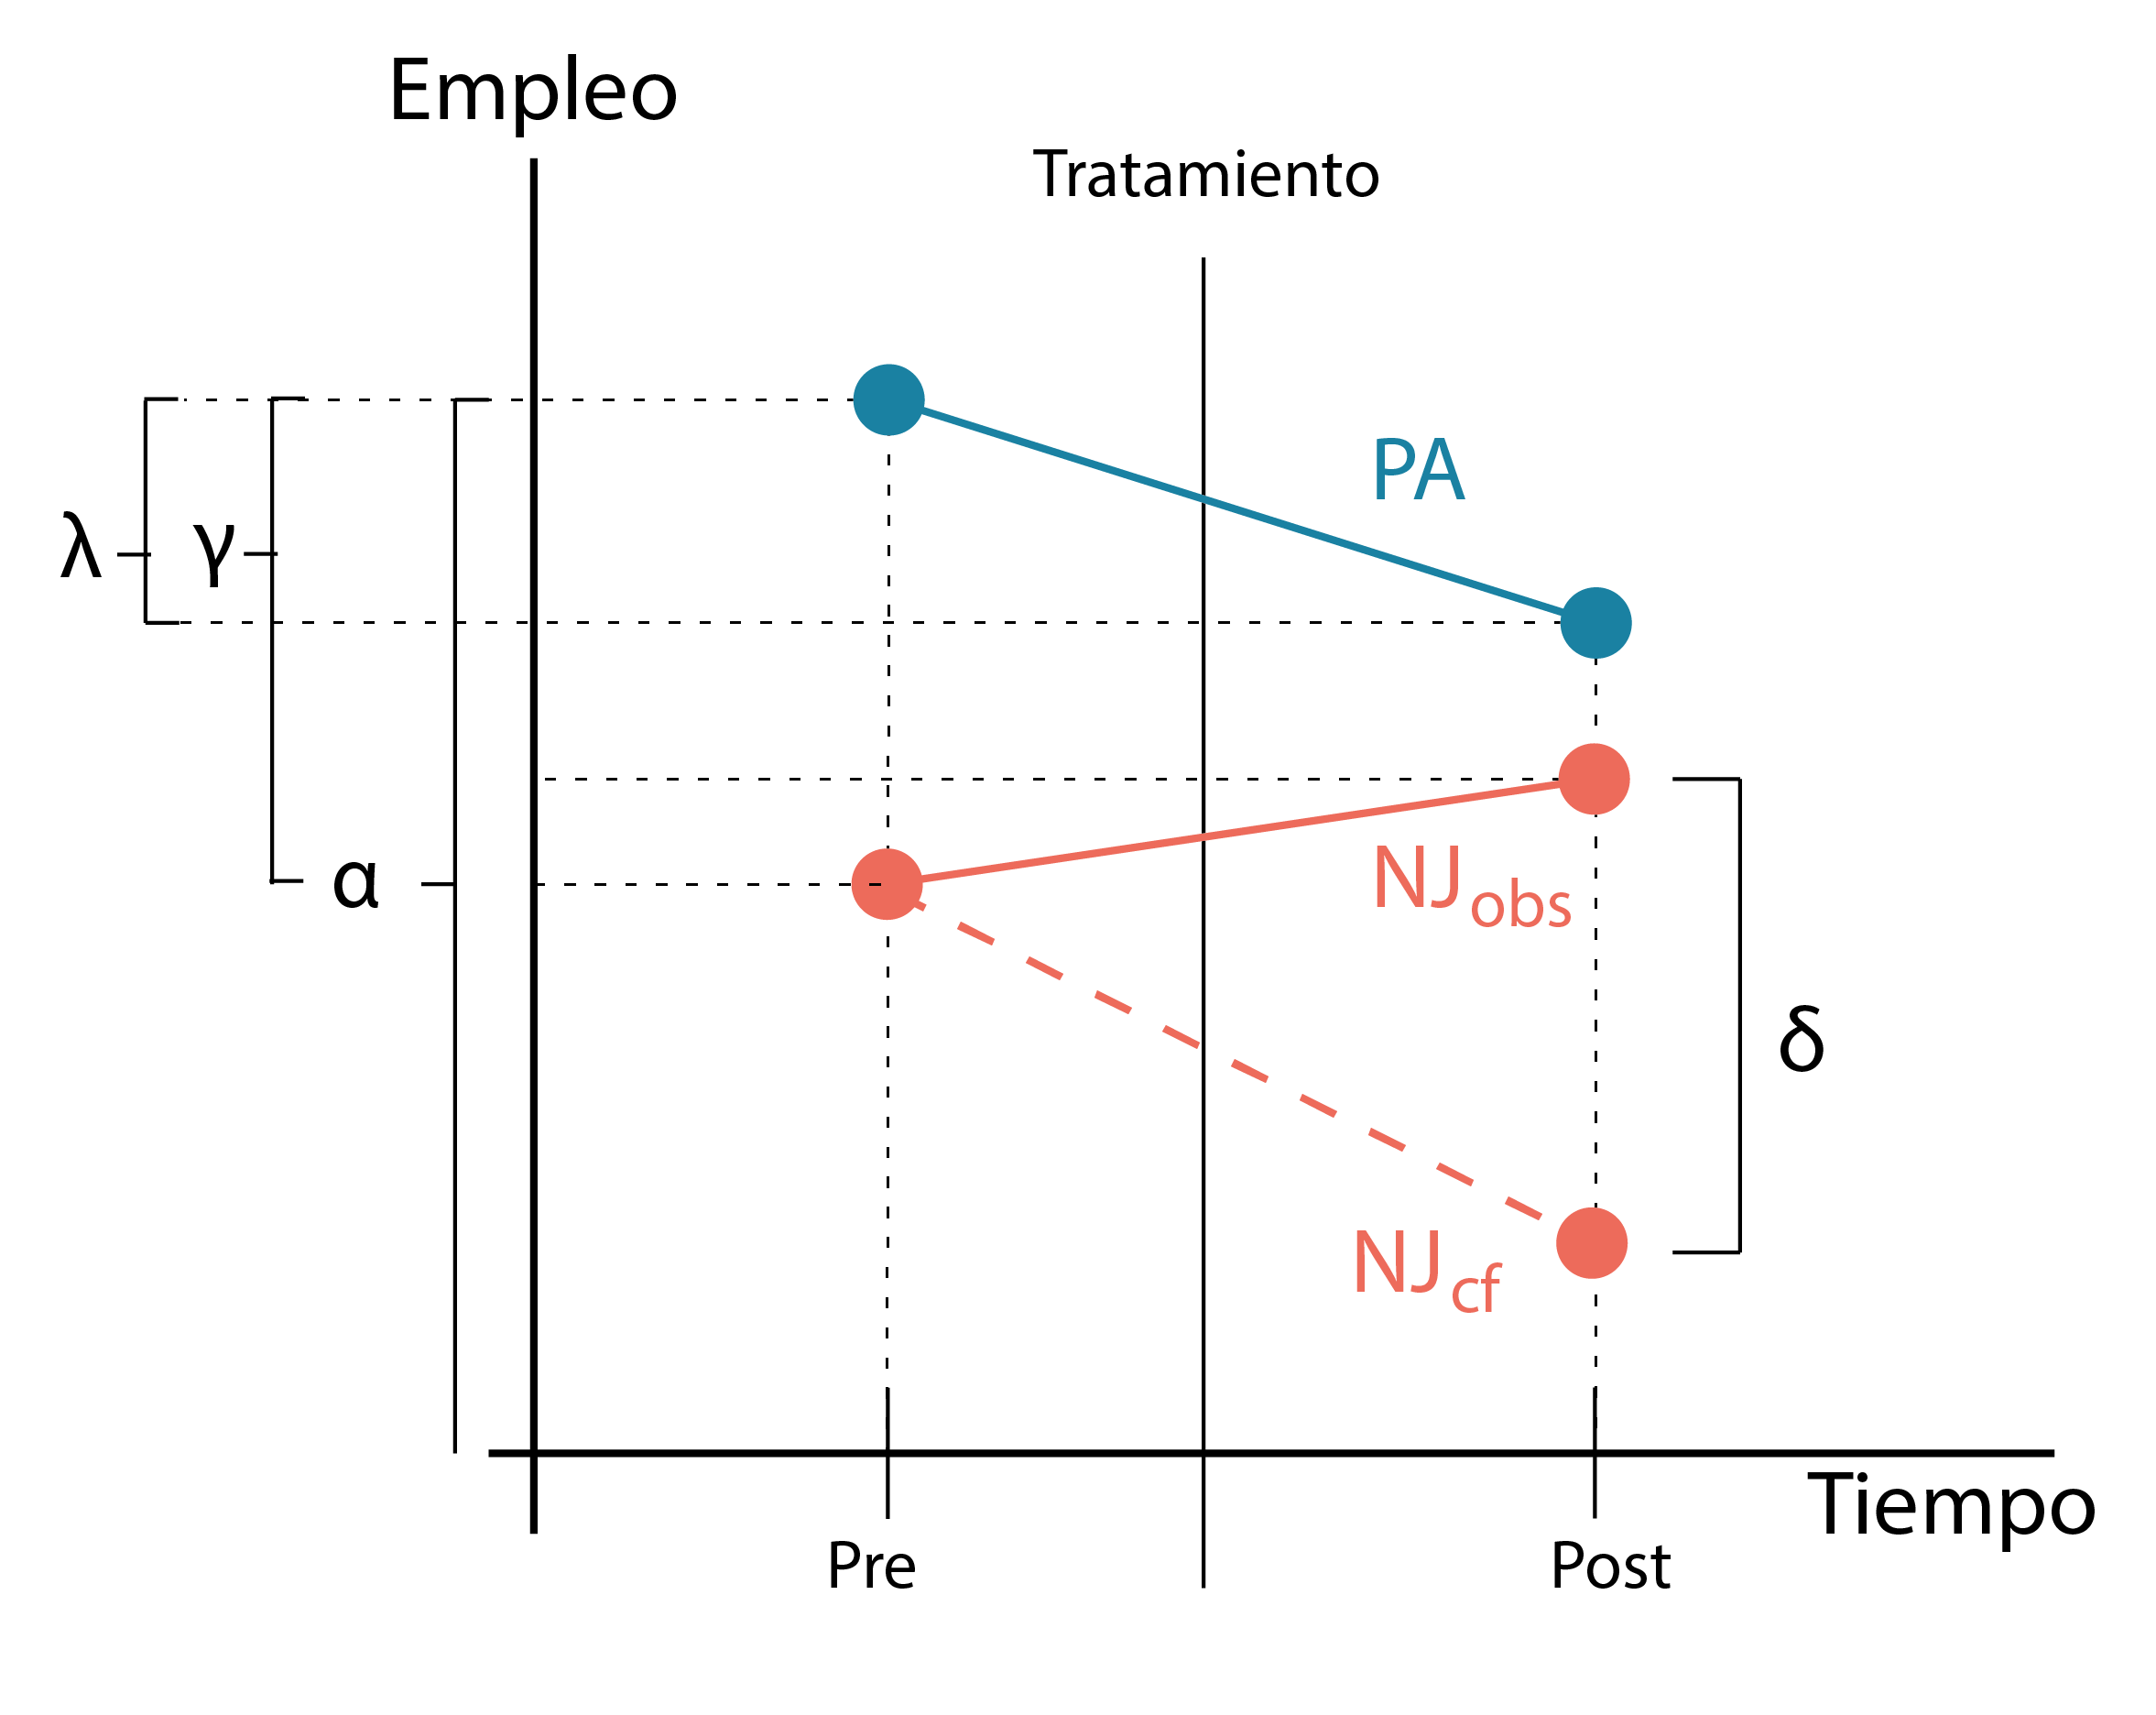
\includegraphics{./imgs/DiD_Mesa de trabajo 1.png}

}

\end{figure}

Si miramos cuidadosamente el parametro \(\delta\) podemos ver como no es
otro más que el ATT ya que es la distancia entre el valor que adopta NJ
en el post tratamiento (en la linea solida) con respecto al valor
contrafactico que hubiera adoptado sin tratamiento (la linea punteada)
ya que si volvemos a nuestra ecuacion esto sería asi:

\$\$

\delta = E{[}Y\^{}1\_\text{NJ} \mid \text{post}{]} -
E{[}Y\^{}0\_\text{NJ}\mid \text{post}{]}

\$\$ Donde el primer termino es observado (porque \(Y=Y^1\), es decir la
medida post tratamiento de NJ que recibio el tratamiento) y el segundo
termino no por la misma razon

Ahora viene lo importante, una regresión lineal escrita a partir del
diseño 2x2DiD siempre estimará la línea punteada, incluso si la
pendiente contrafactual hubiera sido otra. Esto ocurre porque la
regresion lineal utiliza el cambio en el tiempo de Pensilvania para
proyectar un punto a partir del valor previo al tratamiento de Nueva
Jersey. Una vez que se ha llenado ese valor faltante, el estimador del
parámetro es igual a la diferencia entre el valor observado tras el
tratamiento y el valor proyectado, calculado según la pendiente de
Pensilvania, sin importar si esa pendiente de Pensilvania era o no el
referente correcto para medir la pendiente contrafactual de Nueva
Jersey. En resumen, esta regresión siempre estima un tamaño de efecto
usando la pendiente del grupo no tratado como contrafactual, sin
importar si esa pendiente es realmente la adecuada.

Pero, si la pendiente de Pensilvania es igual a la pendiente
contrafactual de Nueva Jersey: en ese caso, la pendiente de Pensilvania
utilizada en la regresión estimará mecánicamente el ATT.

Ahora como venimos viendo, este analisis asume que la pendiente del
contrafactico del grupo tratamiento es paralela a la pendiente del grupo
control. Si esto no ocurriera exactamente así el escenario sería este.

\begin{figure}

{\centering 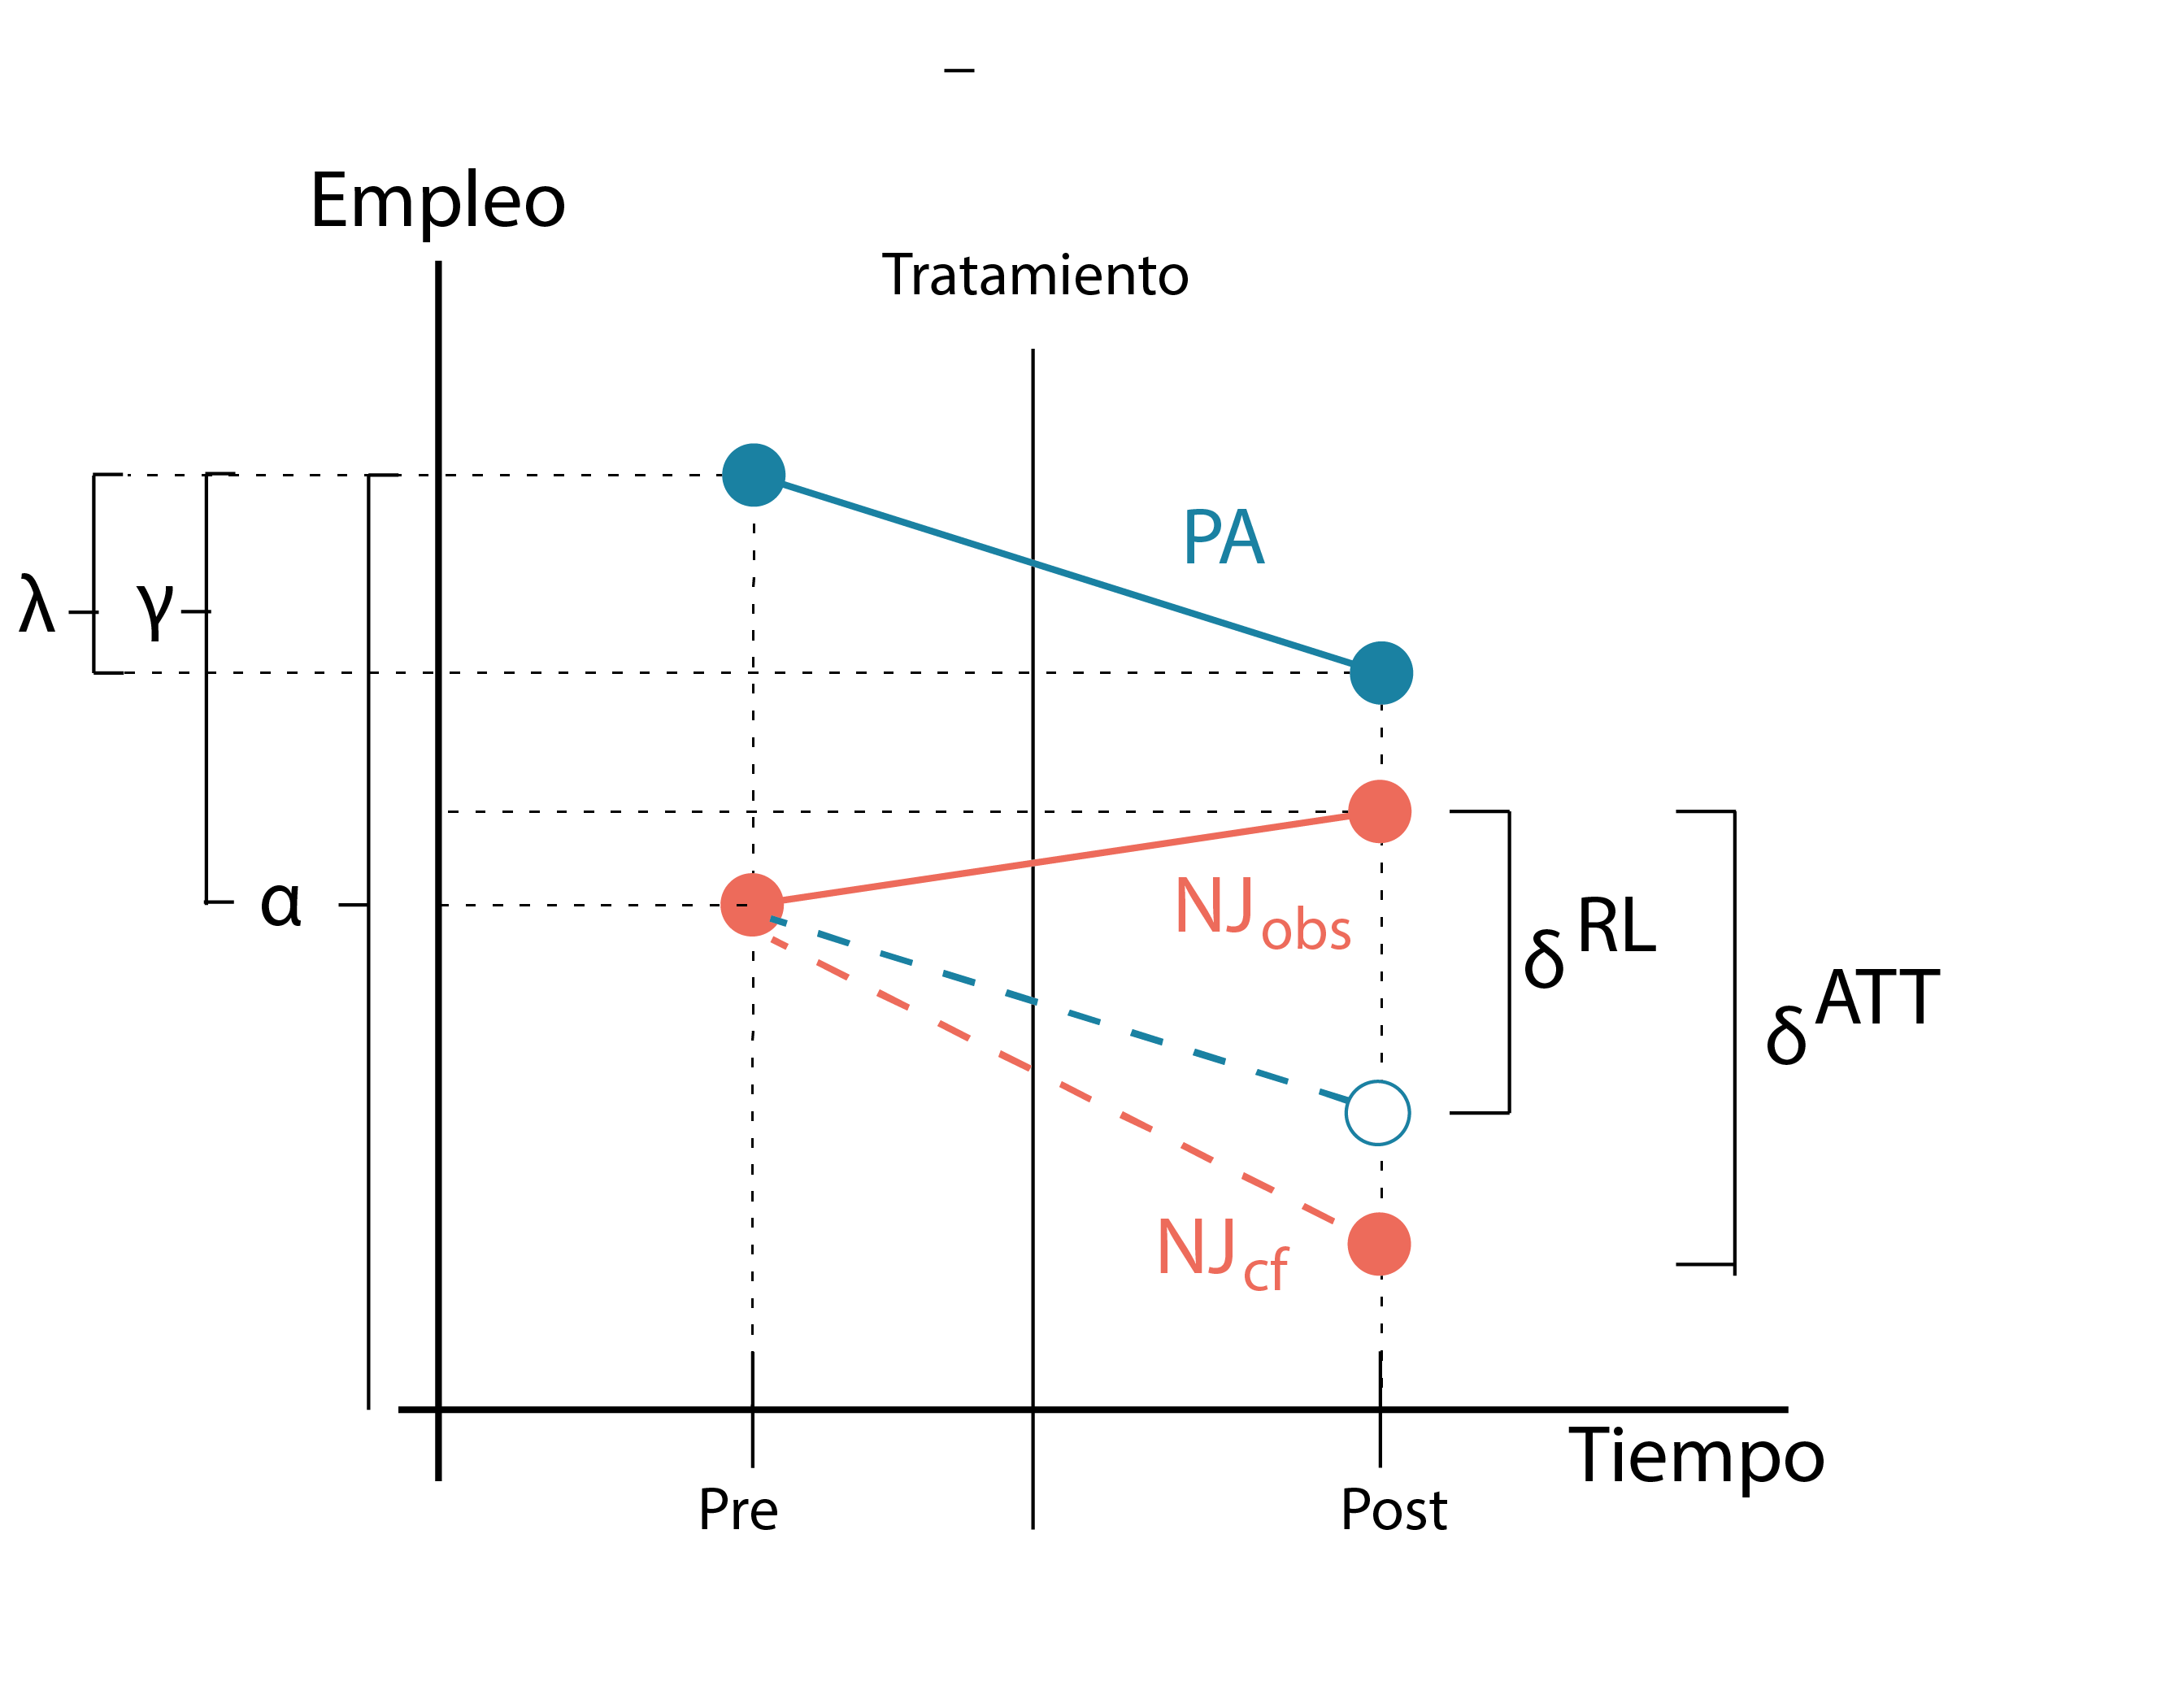
\includegraphics{./imgs/DiD-02.png}

}

\end{figure}

En la figura vemos entonces que la regresión estimo un punto
contrafactico basado en la pendiente de PA (el grupo control), que
podemos ver en azul en ese caso lo cual un estima un parametro
\(\hat{\delta}^\text{RL}\) que es distinto del verdadero efecto causal
dado por el estimador del ATT (nuestro parametro
\(\hat{\delta}^\text{ATT}\)) que es la distancia entre la observacion de
NJ y el contractico real de NJ si no hubiera recibido el tratamiento.

Aquí vemos la importancia del \textbf{supuesto de tendencias paralelas}.
La única situación en la que la estimación de la regresión es igual al
ATT es cuando el contrafactual de Nueva Jersey coincide por casualidad
con la línea punteada de la regresión, que es una línea paralela a la
pendiente de Pensilvania. Y aquí es donde surge el escepticismo
comprensible de muchos observadores: ¿por qué deberíamos basar la
estimación en esta creencia en una coincidencia? Al fin y al cabo,
estamos hablando de una tendencia contrafactual, y por lo tanto no
observable, dado que nunca ocurrió. Tal vez el contrafactual habría
seguido la línea de la regresión, o tal vez habría sido alguna otra
línea desconocida. Podría haber sido cualquier cosa ---simplemente no lo
sabemos.

Por eso se puede decir que el \textbf{supuesto de tendencias paralelas}
es, en realidad, simplemente otra forma de expresar el \textbf{supuesto
de exogeneidad estricta}

\begin{tcolorbox}[enhanced jigsaw, breakable, colback=white, rightrule=.15mm, opacityback=0, colframe=quarto-callout-color-frame, bottomrule=.15mm, left=2mm, toprule=.15mm, leftrule=.75mm, arc=.35mm]
El supuesto de exogeneidad estricta establece que los errorers (o
términos no observados) del modelo no están correlacionados con las
variables explicativas (regresores), y en el caso especial de las DiD,
en ningún período de tiempo.
\end{tcolorbox}

Al decidir optar por un diseño DiD debemos asumir esta condición, porque
no tenemos forma de deducir cuanto esta de lejos un contrafactual (el
que determina la regresión) del contrafactico real. Basicamente porque
ambos son conrafacticos y no medibles. Lo que decimos al apelar a las
tendencias paralelas es que hemos encontrado un grupo de control que
aproxima la trayectoria que habría seguido el grupo tratado, y que el
tratamiento no es endógeno (es decir que el tratamiento no es producto
de las condiciones internas del grupo). Si el tratamiento es endógeno,
entonces las tendencias paralelas se violan siempre, porque en el
contrafactual el grupo tratado habría divergido de todos modos,
independientemente del tratamiento.

Como dijimos esta situacion es inmedible, es una asuncion, es decir
necesita un \emph{salto de fe} y creer que la pendiente del grupo
control es igual (o muy aproximada) a la pendiente del grupo tratamiento
si no hubiera recibido el tratamiento (el contrafactico real). Pero como
todo salto de fe, bueno este puede tener un poco o nada de evidencia a
su favor. Veamos como podemos abordar este problema

\hypertarget{evidencia-a-favor-del-supuesto-de-pendientes-paralelas}{%
\subsection{Evidencia a favor del supuesto de pendientes
paralelas}\label{evidencia-a-favor-del-supuesto-de-pendientes-paralelas}}

Dada la importancia crítica del supuesto de tendencias paralelas para
identificar efectos causales con el diseño de diferencias en diferencias
(DiD), y dado que una de las observaciones necesarias para evaluar dicho
supuesto no está disponible para el investigador, uno podría rendirse y
tirar la toalla. Sin embargo hay un par de metodos para \emph{agregar
evidencia razonable} acerca del supuesto. Vamos a ver dos:

\begin{itemize}
\item
  Estudio de eventos
\item
  Chequeo del balance pretratamiento entre grupos
\end{itemize}

\hypertarget{estudio-de-eventos-previos}{%
\subsubsection{Estudio de eventos
previos}\label{estudio-de-eventos-previos}}

Volvamos a rescribirla formula de nuestro diseño

\[
\hat{\delta}^{\text{2x2}}_{\text{kU}} = 
\underbrace{\left( E[Y^1_k \mid \text{post}] - E[Y^0_k \mid \text{post}] \right)}_{\text{ATT}} + 
\underbrace{\left[ \left( E[Y^0_k \mid \text{post}] - E[Y^0_k \mid \text{pre}] \right) - \left( E[Y^0_U \mid \text{post}] - E[Y^0_U \mid \text{pre}] \right) \right]}_{\text{Bias due to non-parallel trends in 2x2}}
\]

Nos interesa el primer término, el ATT, pero este se ve contaminado por
sesgo de selección cuando el segundo término no es igual a cero. Como
evaluar el segundo término requiere el contrafactual, \$
E{[}Y0∣post,D=1{]}−E{[}Y0∣pre,D=1{]}E{[}Y0∣post,D=1{]}−E{[}Y0∣pre,D=1{]}\$,
no podemos hacerlo directamente. Lo que que si se puede hacer, en
cambio, es comparar coeficientes placebo de DD en los períodos previos
al tratamiento. Si los coeficientes DD en esos períodos pretratamiento
son estadísticamente iguales a cero, entonces las diferencias en
diferencias entre el grupo tratado y el de control siguieron una
tendencia similar antes del tratamiento.

\begin{figure}

{\centering 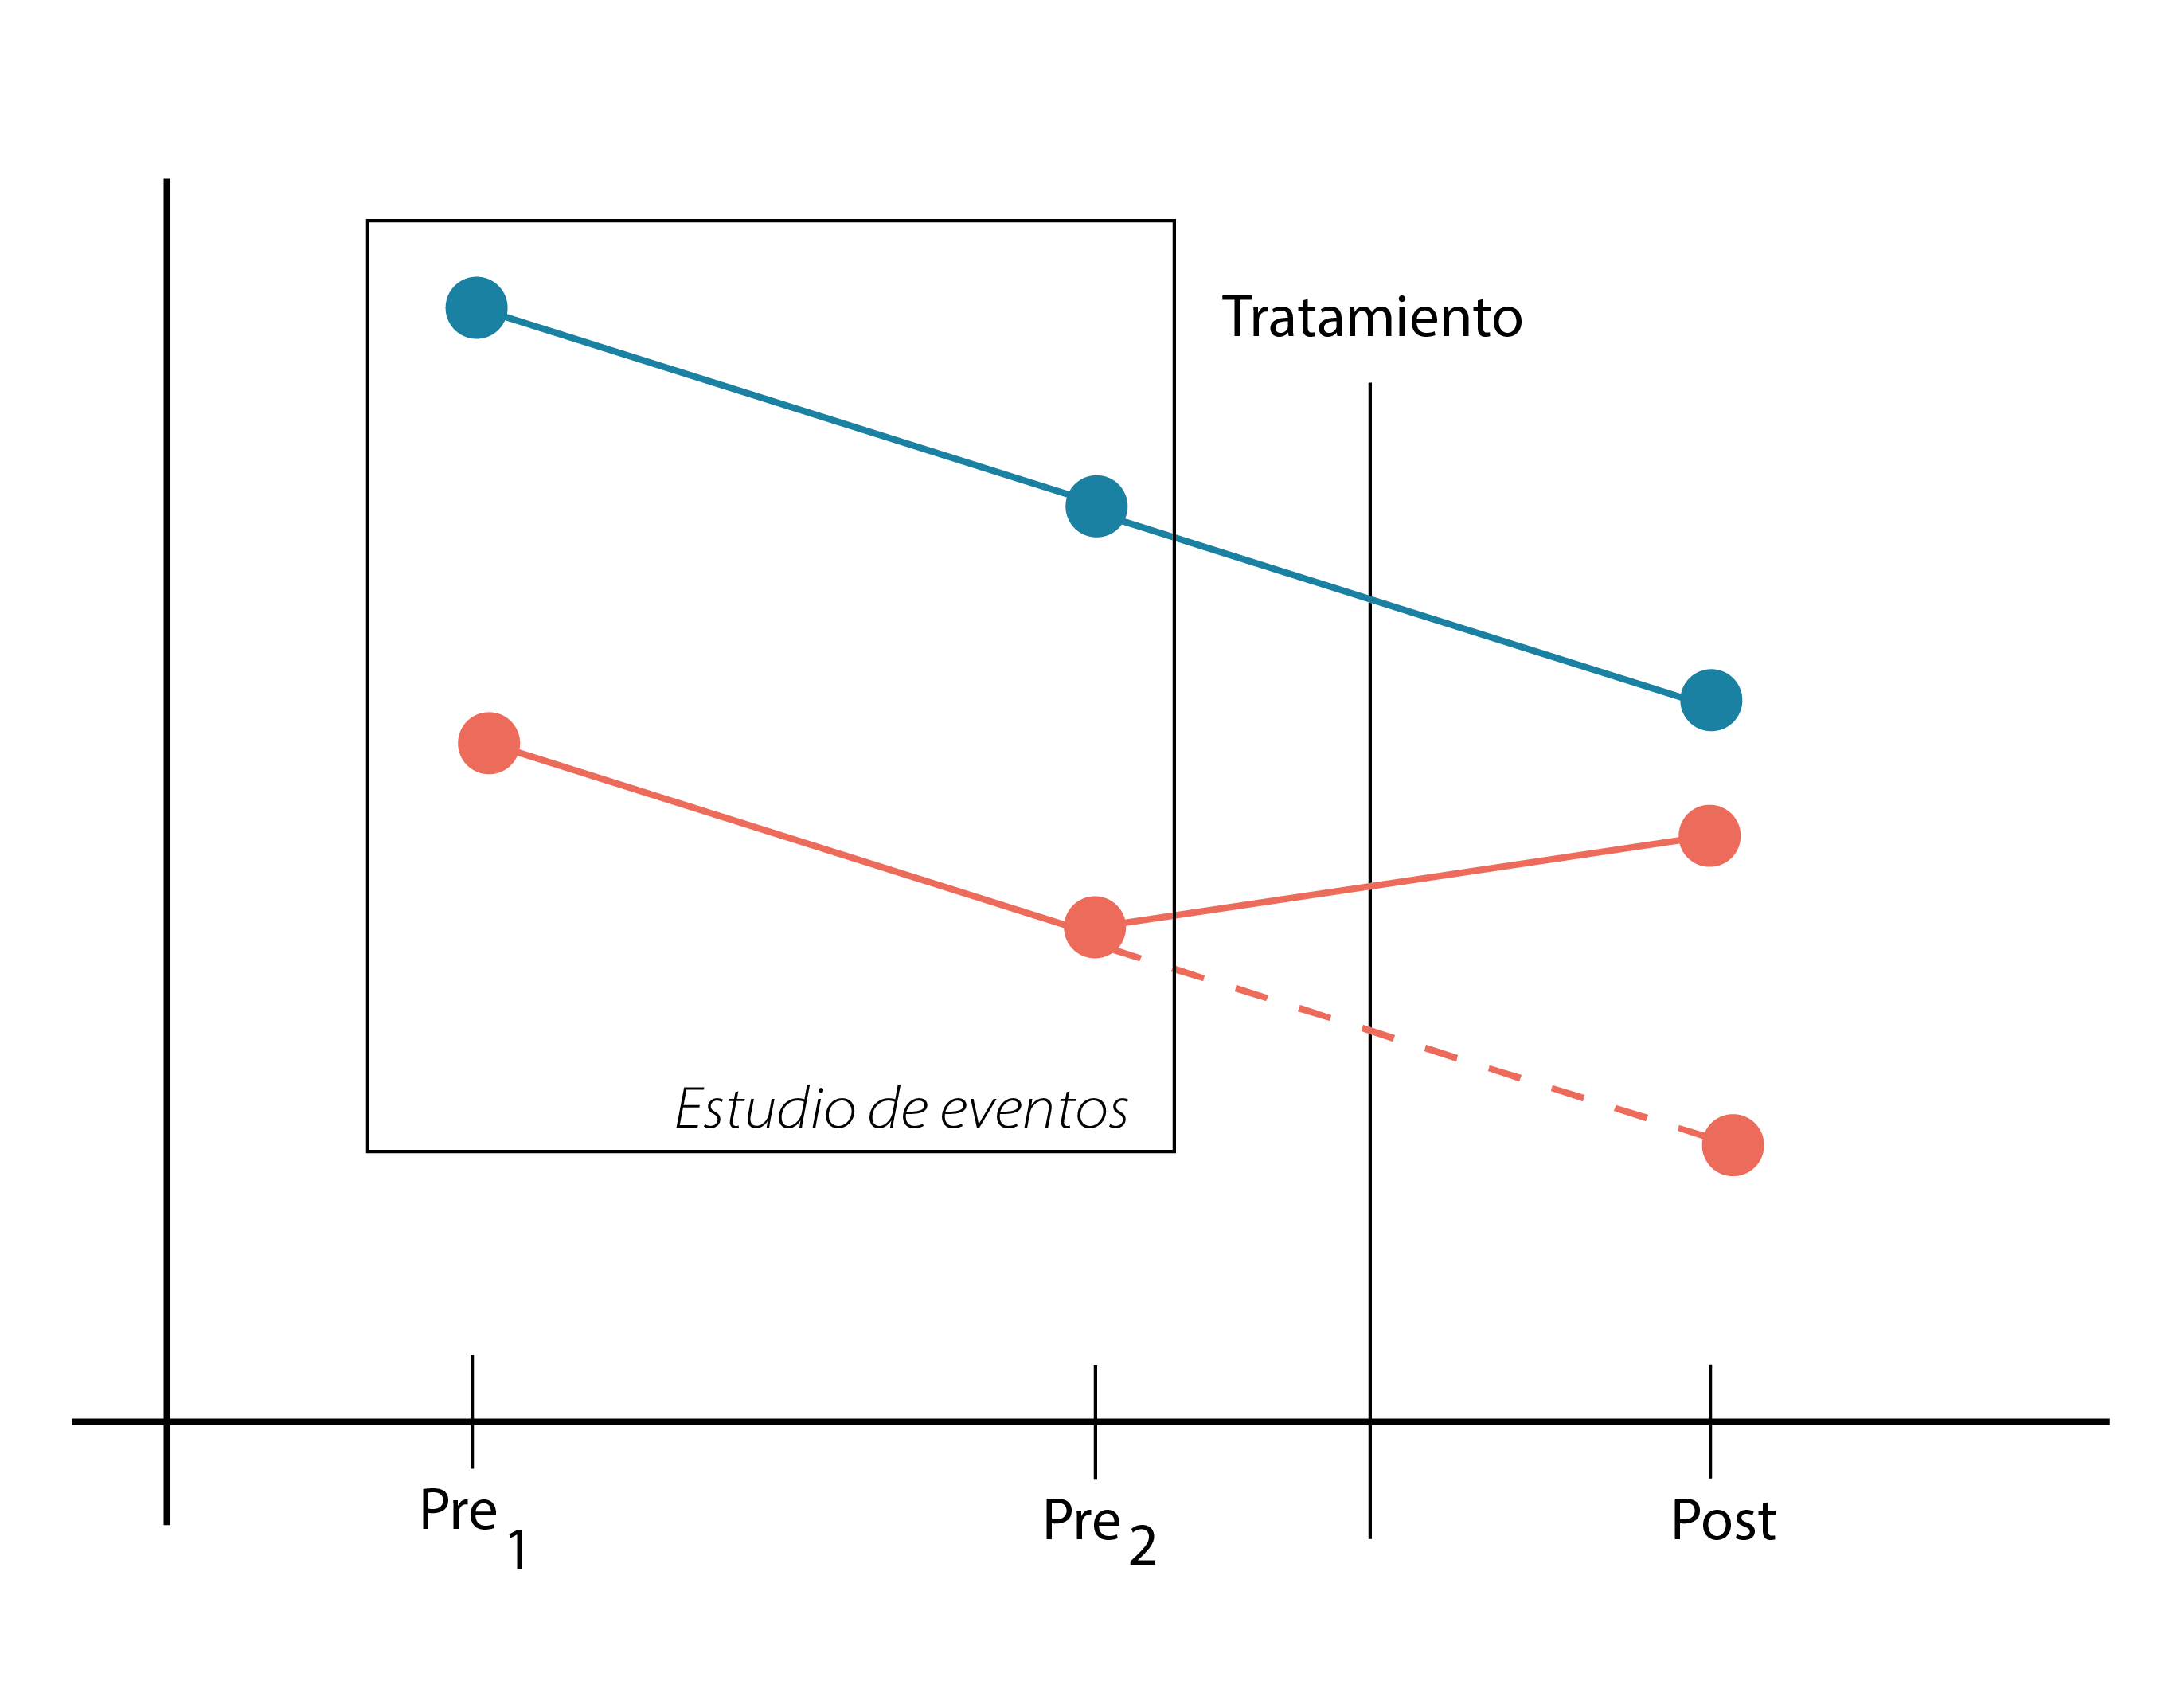
\includegraphics{./imgs/DiD-04.png}

}

\end{figure}

Y aquí aparece el arte retórico del diseño: si fueron similares antes,
¿por qué no habrían de continuar siéndolo después del tratamiento?

Pero esta retórica es una especie de prueba por afirmación. Que hayan
sido similares antes no implica lógicamente que deban serlo después.
Asumir que el futuro será como el pasado es una forma de la falacia del
jugador conocida como la ``posición inversa''. Que una moneda haya
salido cara tres veces seguidas no significa que deba salir cara la
cuarta vez, al menos no sin otros supuestos adicionales. De la misma
forma, no estamos obligados a creer que las tendencias contrafactuales
serían iguales tras el tratamiento solo porque lo fueron antes, salvo
que hagamos más supuestos sobre el poder predictivo de las tendencias
previas. Pero hacer tales supuestos es, nuevamente, hacer supuestos no
comprobables, y así volvemos al punto de partida.

Un caso en el que las tendencias paralelas se violarían de forma
evidente es cuando el tratamiento es endógeno. En ese escenario, la
asignación al tratamiento dependería directamente de los resultados
potenciales y, en ausencia del tratamiento, esos resultados habrían
cambiado de todas formas. Tal endogeneidad tradicional requiere más que
simples visualizaciones ``perezosas'' de las tendencias previas. Aunque
la prueba de placebo es importante, técnicamente las similitudes
pretratamiento no son necesarias ni suficientes para garantizar
tendencias contrafactuales paralelas (Kahn-Lang y Lang 2019). El
supuesto no se prueba tan fácilmente. Nunca se puede dejar de ser
riguroso al intentar determinar si los grupos se seleccionaron
endógenamente al tratamiento, si hay sesgos por variables omitidas,
distintas fuentes de sesgo de selección o caminos de retroceso abiertos.
Cuando el término de error estructural en un modelo de regresión
dinámica no está correlacionado con la variable de tratamiento, se tiene
exogeneidad estricta, y eso es lo que proporciona las tendencias
paralelas y permite hacer afirmaciones significativas sobre las
estimaciones.

\hypertarget{mostrar-el-balance-pretratamiento-de-ambos-grupos}{%
\subsubsection{Mostrar el balance pretratamiento de ambos
grupos}\label{mostrar-el-balance-pretratamiento-de-ambos-grupos}}

Recien mencionamos que estudiar los eventos previos es una forma
(indirecta) de juntar evidencia a favor de este supuesto de tendencias
paralelas (para que el salto de fe no sea tan alto) El problema es que
como analizamos eso?, bueno hay varios enfoques que podemos tomar, en
conjunto se los suele llamar \emph{event study plots} Una forma simple
de conducir esto es graficar los datos pretratamiento (como en en la
figura anterior), sin embargo esto requiere que tengamos mucha suerte y
los datos se hayan tomado en forma fija en otros eventos. Estos datos
que provienen de observaicones rara vez suelen comportarse asi

Un escenario mucho más común es la existencia de un \emph{timing
diferencial}, en el que los grupos de unidades adoptan el tratamiento en
distintos momentos. Entonces el concepto de ``pretratamiento'' se vuelve
complejo. En nuestro ejemplo para el caso, Nueva Jersey aumentó su
salario mínimo en 1992 y Nueva York lo hizo en 1994, pero Pensilvania
nunca aumentó su salario mínimo, el período previo al tratamiento se
define para Nueva Jersey (1991) y para Nueva York (1993), pero no para
Pensilvania. Entonces, ¿cómo probamos las diferencias previas al
tratamiento en ese caso? La gente lo ha hecho de varias maneras.

Una posibilidad es graficar los datos brutos, año por año, y simplemente
observar a ojo. Compararías el grupo tratado con el nunca tratado, por
ejemplo, lo que podría requerir muchos gráficos y ser visualmente
incómodo.La ventaja es que muestra de forma transparente los datos
crudos sin ajustes. Sin trucos. Las desventajas son varias. Primero,
puede ser engorroso cuando el número de grupos tratados es grande,
volviéndolo prácticamente imposible. Segundo, puede que no sea
visualmente atractivo. Y tercero, este enfoque asume necesariamente que
el único grupo de control es el nunca tratado, lo que en realidad no es
cierto. Cualquier DiD es una combinación de una comparación entre
tratados y nunca tratados, tratados tempranos (a los que llamaremos
\textbf{leads}) frente a tratados tardíos (a los que llamaremos
\textbf{lags}) y tratados tardíos frente a tratados tempranos. Por lo
tanto, mostrar solo la comparación con los nunca tratados es en realidad
una presentación engañosa del mecanismo de identificación subyacente en
un modelo de efectos fijos bidireccionales con timing diferencial.

La forma actual en que se evalúan las dinámicas previas al tratamiento
entre un grupo tratado y uno de control con timing diferencial es
estimar un modelo de regresión que incluya \emph{leads} y \emph{lags}
del tratamiento. Un ejemplo de eso puede ser graficar los leads previos
al tratamiento en lugar de graficar tratamiento y control y tras la
estimacion graficar los intervalos de regresion en cada unidad de
leads/lags. Los modelos como estos suelen seguir una forma asi:

\[
Y_{its} = \gamma_s + \lambda_t + \sum_{\tau=-q}^{-1} \gamma_{\tau} D_{s\tau} + \sum_{\tau=0}^{m} \delta_{\tau} D_{s\tau} + x_{ist} + \varepsilon_{ist}
\] El tratamiento ocurre en el año 0. Se incluyen \(q\) leads o efectos
anticipatorios, y \(m\) lags o efectos posteriores al tratamiento. Ete
tipo de enfoques permite al al lector comprobar tanto el grado en que
los efectos del tratamiento post-tratamiento fueron dinámicos, como si
los dos grupos eran comparables en sus dinámicas del resultado antes del
tratamiento.

\hypertarget{la-importancia-delplacebo}{%
\section{La importancia delplacebo}\label{la-importancia-delplacebo}}

Existen varias pruebas para evaluar la validez de una estrategia de
difference-in-differences (DD). Ya he mencionado una: la comparabilidad
entre los grupos de tratamiento y control en las dinámicas observables
antes del tratamiento. Ahora hablaré de otras formas creíbles de evaluar
si los efectos causales estimados son fiables, destacando el uso de
falsificación mediante placebos.

La idea de la falsificación con placebos es sencilla. Supongamos que
encuentras un efecto negativo del salario mínimo sobre el empleo de los
trabajadores con salarios bajos. ¿Es verdadera la hipótesis si
encontramos evidencia a favor? Quizás sí, quizás no. Lo que realmente
podría ayudar sería tener en mente una hipótesis alternativa e intentar
ponerla a prueba. Si no puedes rechazar la hipótesis nula en esa
hipótesis alternativa, eso aporta credibilidad a tu análisis original.
Por ejemplo, puede que estés captando algo espurio, como factores
cíclicos u otros no observables que no se capturan fácilmente con
efectos fijos de tiempo o de estado. Entonces, ¿qué puedes hacer?

Un candidato para la falsificación con placebo podría ser simplemente
usar datos de un tipo alternativo de trabajador cuyos salarios no se
vean afectados por el salario mínimo vinculante. Por ejemplo, los
salarios mínimos afectan el empleo y las ganancias de los trabajadores
con salarios bajos, ya que estos son los trabajadores contratados
literalmente con base en el salario de mercado. Sin un serio equilibrio
general de por medio, el salario mínimo no debería afectar el empleo de
los trabajadores con salarios altos, porque el salario mínimo no es
vinculante para ellos. Dado que los trabajadores de salarios altos y
bajos suelen estar empleados en sectores muy distintos, es poco probable
que sean sustitutos. Este razonamiento podría llevarnos a considerar que
los trabajadores con salarios altos funcionen como un placebo.

Hay dos formas de incorporar esta idea en nuestro análisis. A muchos les
gusta ser directos y simplemente ajustar el mismo diseño DD usando como
variable de resultado el empleo de los trabajadores con salarios altos.
Si el coeficiente del salario mínimo es cero cuando usamos el empleo de
trabajadores con salarios altos como resultado, pero el coeficiente del
salario mínimo para los trabajadores con salarios bajos es negativo,
entonces habremos aportado una evidencia más sólida que complementa el
análisis previo de los trabajadores con salarios bajos. Pero hay otro
método que utiliza el placebo dentro del estado para la identificación,
llamado difference-in-differences-in-differences (o ``triple
differences''), que no abordaremos aqui

\bookmarksetup{startatroot}

\hypertarget{sec-random-exp}{%
\chapter{Regresión discontinua}\label{sec-random-exp}}

\hypertarget{el-problema-de-controlar-por-variables-no-observables}{%
\section{El problema de controlar por variables no
observables}\label{el-problema-de-controlar-por-variables-no-observables}}

En la mayoría de los capítulos anteriores, vimos formas de controlar por
confusores observables. Cuando hablamos de DAGs y agregar variables como
covariables a un modelo de regresión o cuando usamos algún estimador de
subclasificación o \emph{matching}, lo que estamos haciendo es aislar la
variabilidad debida a confusores observados y sustraerla de nuestra
relación causal. Pero, ¿Qué pasa cuando los confusores por los que
queremos controlar no son observables? Una respuesta a esta pregunta la
tuvimos en el capítulo de diferencias en diferencias en el que vimos
que, para un problema de una forma en particular\sidenote{\footnotesize Un problema
  con un tratamiento que se aplica en el tiempo y para el cual tenemos
  una medición antes y después para un grupo al que se le aplicó el
  tratamiento y una medición para los mismos puntos temporales pero para
  un grupo comparable (para más detalles ver el
  \textbf{?@sec-diff-in-diff}).}, la solución era estimar el
contrafáctico con un grupo comparable.

La solución que vamos a proponer en este capítulo, al igual que en
diferencias en diferencias, utiliza el contexto de mi cuasiexperimento
para aislar el efecto causal.

\hypertarget{one-rule-to-rule-them-all}{%
\section{\texorpdfstring{\emph{One rule to rule them
all}}{One rule to rule them all}}\label{one-rule-to-rule-them-all}}

La idea básica detrás de la regresión discontinua es que la separación
entre grupo tratamiento y control está dada por una discontinuidad en
alguna variable\sidenote{\footnotesize Que a partir de ahora llamaremos \emph{running
  variable}.}. Es decir, a partir de un cierto valor de esta variable un
sujeto es asignado a un determinado grupo. Por ejemplo, a partir un
valor de ingreso mensual, un individuo podría tener acceso a un programa
de ayuda social. Supongamos que ese límite es \$\(350000\) mensuales.
¿En qué se diferencian dos individuos que cobran \$\(349999\) y
\$\(350001\) respectivamente? Probablemente en mucho, ¿no? Pero ¿y si
comparamos \(100\) individuos de cada ingreso? Es bastante razonable
pensar que en todas las demás características, estos individuos son
comparables. Es decir, que la única diferencia entre ellos es que uno de
ellos accede a un programa social y el otro no. Bueno, es en esta idea
en la que se cimenta (ah bueno, se puso fino el autor) la regresión
discontinua. En líneas generales vamos a comprar unidades experimentales
cerquita de un lado del umbral de la \emph{running variable} con
unidades experimentales cerquita del otro lado del umbral.

Empecemos a jugar con un ejemplo con datos simulados. En este ejemplo
tenemos datos de la asignación de estudiantes de un curso de estadística
a un programa de tutorías. La cosa es así: Los estudiantes se someten a
un examen inicial y dependiendo de su puntaje, son asignados a un
programa de tutorías o no. El umbral para la asignación es un puntaje de
\(70\) puntos. Si el estudiante saca menos de \(70\) puntos, participa
del programa de tutorías. Si saca \(70\) o más, no participa. Luego, a
cada estudiante se le evalúa con un examen final. La pregunta que nos
hacemos es: ¿El programa de tutorías mejora el puntaje en el examen
final? Veamos qué pinta tienen los datos viendo las primeras 5 filas del
dataset.

\begin{Shaded}
\begin{Highlighting}[]
\NormalTok{tutoring }\OtherTok{\textless{}{-}} \FunctionTok{read\_csv}\NormalTok{(}\FunctionTok{here}\NormalTok{(}\StringTok{"data/tutoring\_program.csv"}\NormalTok{)) }\SpecialCharTok{\%\textgreater{}\%} 
  \FunctionTok{mutate}\NormalTok{(}\AttributeTok{tutoring =} \FunctionTok{factor}\NormalTok{(tutoring, }\AttributeTok{levels =} \FunctionTok{c}\NormalTok{(}\ConstantTok{FALSE}\NormalTok{, }\ConstantTok{TRUE}\NormalTok{), }
                           \AttributeTok{labels =} \FunctionTok{c}\NormalTok{(}\StringTok{"No"}\NormalTok{, }\StringTok{"Sí"}\NormalTok{)))}
\CommentTok{\#\textgreater{} Rows: 1000 Columns: 4}
\CommentTok{\#\textgreater{} {-}{-} Column specification {-}{-}{-}{-}{-}{-}{-}{-}{-}{-}{-}{-}{-}{-}{-}{-}{-}{-}{-}{-}{-}{-}{-}{-}{-}{-}{-}{-}{-}{-}{-}{-}{-}{-}{-}{-}{-}{-}{-}{-}{-}{-}{-}{-}{-}{-}{-}{-}{-}{-}{-}{-}{-}}
\CommentTok{\#\textgreater{} Delimiter: ","}
\CommentTok{\#\textgreater{} dbl (3): id, entrance\_exam, exit\_exam}
\CommentTok{\#\textgreater{} lgl (1): tutoring}
\CommentTok{\#\textgreater{} }
\CommentTok{\#\textgreater{} i Use \textasciigrave{}spec()\textasciigrave{} to retrieve the full column specification for this data.}
\CommentTok{\#\textgreater{} i Specify the column types or set \textasciigrave{}show\_col\_types = FALSE\textasciigrave{} to quiet this message.}

\NormalTok{tutoring }\SpecialCharTok{\%\textgreater{}\%}
  \FunctionTok{head}\NormalTok{() }\SpecialCharTok{\%\textgreater{}\%}
  \FunctionTok{gt}\NormalTok{()}
\end{Highlighting}
\end{Shaded}

\begin{table}
\fontsize{12.0pt}{14.4pt}\selectfont
\begin{tabular*}{\linewidth}{@{\extracolsep{\fill}}rrrc}
\toprule
id & entrance\_exam & exit\_exam & tutoring \\ 
\midrule\addlinespace[2.5pt]
1 & 92.4 & 78.1 & No \\ 
2 & 72.8 & 58.2 & No \\ 
3 & 53.7 & 62.0 & Sí \\ 
4 & 98.3 & 67.5 & No \\ 
5 & 69.7 & 54.1 & Sí \\ 
6 & 68.1 & 60.1 & Sí \\ 
\bottomrule
\end{tabular*}
\end{table}

Por ejemplo, vemos que el estudiante de la primera fila tiene un puntaje
de \(92.4\) puntos en el examen de entrada y, efectivamente, no
participa en el programa de tutorías. Por otro lado, el estudiante de la
tercera fila, con sus magros \(53.7\) puntos en el examen de entrada, sí
participó del programa de tutorías.

Veamos las notas de entrada y como afecta eso a la participación en las
tutorías:

\begin{Shaded}
\begin{Highlighting}[]
\NormalTok{rect\_claro }\OtherTok{\textless{}{-}} \FunctionTok{tibble}\NormalTok{(}\AttributeTok{xmin =} \DecValTok{65}\NormalTok{, }\AttributeTok{xmax =} \DecValTok{75}\NormalTok{, }\AttributeTok{ymin =} \DecValTok{0}\NormalTok{, }\AttributeTok{ymax =} \DecValTok{3}\NormalTok{)}

\FunctionTok{ggplot}\NormalTok{(tutoring) }\SpecialCharTok{+}
  \CommentTok{\# Los rectángulos}
  \FunctionTok{geom\_rect}\NormalTok{(}\AttributeTok{data =}\NormalTok{ rect\_claro, }\FunctionTok{aes}\NormalTok{(}\AttributeTok{xmin =}\NormalTok{ xmin, }\AttributeTok{xmax =}\NormalTok{ xmax, }\AttributeTok{ymin =}\NormalTok{ ymin, }\AttributeTok{ymax =}\NormalTok{ ymax), }
            \AttributeTok{fill =} \StringTok{"gray20"}\NormalTok{, }\AttributeTok{color =} \StringTok{"white"}\NormalTok{, }\AttributeTok{alpha =}\NormalTok{ .}\DecValTok{2}\NormalTok{) }\SpecialCharTok{+}
  \CommentTok{\# Hacemos los puntos semitransparentes y los movemos un poco}
  \FunctionTok{geom\_point}\NormalTok{( }\FunctionTok{aes}\NormalTok{(}\AttributeTok{x =}\NormalTok{ entrance\_exam, }
                  \AttributeTok{y =}\NormalTok{ tutoring, }
                  \AttributeTok{color =}\NormalTok{ tutoring),}
              \AttributeTok{size =} \FloatTok{1.5}\NormalTok{, }\AttributeTok{alpha =} \FloatTok{0.5}\NormalTok{, }
             \AttributeTok{position =} \FunctionTok{position\_jitter}\NormalTok{(}\AttributeTok{width =} \DecValTok{0}\NormalTok{, }\AttributeTok{height =} \FloatTok{0.25}\NormalTok{, }\AttributeTok{seed =} \DecValTok{1234}\NormalTok{)) }\SpecialCharTok{+} 
  \CommentTok{\# Ponemos una línea vertical en el umbral}
  \FunctionTok{geom\_vline}\NormalTok{(}\AttributeTok{xintercept =} \DecValTok{70}\NormalTok{, }\AttributeTok{color =} \StringTok{"yellow"}\NormalTok{, }\AttributeTok{linetype =} \StringTok{"dashed"}\NormalTok{) }\SpecialCharTok{+} 
  \CommentTok{\# Labels}
  \FunctionTok{labs}\NormalTok{(}\AttributeTok{x =} \StringTok{"Puntaje en el examen de entrada"}\NormalTok{, }\AttributeTok{y =} \StringTok{"Participación en el programa de tutorías"}\NormalTok{) }\SpecialCharTok{+} 
  \CommentTok{\# Sacó la leyenda de color}
  \FunctionTok{guides}\NormalTok{(}\AttributeTok{color =} \ConstantTok{FALSE}\NormalTok{) }\SpecialCharTok{+}
  \CommentTok{\# Colores más chetos}
  \FunctionTok{scale\_color\_brewer}\NormalTok{(}\AttributeTok{palette =} \StringTok{"Dark2"}\NormalTok{) }\SpecialCharTok{+}
  \CommentTok{\# Theme sin fondo gris}
  \FunctionTok{theme\_minimal}\NormalTok{()}
\CommentTok{\#\textgreater{} Warning: The \textasciigrave{}\textless{}scale\textgreater{}\textasciigrave{} argument of \textasciigrave{}guides()\textasciigrave{} cannot be \textasciigrave{}FALSE\textasciigrave{}. Use "none" instead}
\CommentTok{\#\textgreater{} as of ggplot2 3.3.4.}
\end{Highlighting}
\end{Shaded}

\begin{figure}[H]

{\centering 
\includegraphics[width=18.75in,height=\textheight]{./reg_discontinua_files/figure-pdf/unnamed-chunk-3-1.pdf}

}

\caption{Efecto de las notas de entrada (la running variable) en la
participación en las tutorías.}

\end{figure}

Vemos claramente que los estudiantes con más de \(70\) puntos en el
examen de entrada no participan del programa de tutorías, mientras que
los que sacaron menos de \(70\) sí. Parece que el umbral divide bastante
bien a los grupos. Pero, pensando de nuevo en el ejemplo del ingreso,
¿qué pasa con los estudiantes que sacaron puntajes cercanos a \(70\)?
¿Son comparables? ¿Podemos asumir que la única diferencia entre ellos es
la participación en el programa de tutorías? Es razonable asumir que sí.

Recordemos que la pregunta era ¿cómo afecta el programa de tutorías a la
nota del examen final de los alumnos? Vamos a ver las notas de entrada y
de salida de cada individuo en un gráfico. En el mismo gráfico vamos a
colorear los puntos según si el estudiante participó o no del programa
de tutorías y vamos a marcar como una línea vertical el umbral de \(70\)
puntos en el examen de entrada.

\begin{Shaded}
\begin{Highlighting}[]
\CommentTok{\# Ahora miremos como se comporta la variable outcomes en función de la running variable \#\#\#\#}
\FunctionTok{ggplot}\NormalTok{(tutoring, }\FunctionTok{aes}\NormalTok{(}\AttributeTok{x =}\NormalTok{ entrance\_exam, }
                     \AttributeTok{y =}\NormalTok{ exit\_exam, }
                     \AttributeTok{color =}\NormalTok{ tutoring,}
                     \AttributeTok{fill =}\NormalTok{ tutoring)) }\SpecialCharTok{+}
  \FunctionTok{geom\_point}\NormalTok{(}\AttributeTok{size =} \FloatTok{1.5}\NormalTok{, }\AttributeTok{alpha =}\NormalTok{ .}\DecValTok{3}\NormalTok{) }\SpecialCharTok{+} 
  \CommentTok{\# Ponemos una línea vertical en el umbral}
  \FunctionTok{geom\_vline}\NormalTok{(}\AttributeTok{xintercept =} \DecValTok{70}\NormalTok{, }\AttributeTok{color =} \StringTok{"steelblue"}\NormalTok{, }\AttributeTok{linetype =} \StringTok{"dashed"}\NormalTok{) }\SpecialCharTok{+} 
  \CommentTok{\# Las lables}
  \FunctionTok{labs}\NormalTok{(}\AttributeTok{x =} \StringTok{"Puntaje en el examen de entrada"}\NormalTok{, }
       \AttributeTok{y =} \StringTok{"Puntaje en el examen de salida"}\NormalTok{,}
       \AttributeTok{color =} \StringTok{"Participó en la tutoría"}\NormalTok{,}
       \AttributeTok{fill =} \StringTok{"Participó en la tutoría"}\NormalTok{) }\SpecialCharTok{+} 
  \CommentTok{\# Colores más chetos}
  \FunctionTok{scale\_color\_brewer}\NormalTok{(}\AttributeTok{palette =} \StringTok{"Dark2"}\NormalTok{) }\SpecialCharTok{+}
  \FunctionTok{scale\_fill\_brewer}\NormalTok{(}\AttributeTok{palette =} \StringTok{"Dark2"}\NormalTok{) }\SpecialCharTok{+}
  \CommentTok{\# Theme sin fondo gris}
  \FunctionTok{theme\_minimal}\NormalTok{() }\SpecialCharTok{+}
  \FunctionTok{theme}\NormalTok{(}\AttributeTok{legend.position =} \StringTok{"top"}\NormalTok{)}
\end{Highlighting}
\end{Shaded}

\begin{figure}[H]

{\centering 
\includegraphics[width=18.75in,height=\textheight]{./reg_discontinua_files/figure-pdf/unnamed-chunk-4-1.pdf}

}

\caption{Notas de entrada vs.~notas de salida.}

\end{figure}

Pareciera que hay una relación entre la nota de entrada y de salida.
Esto tiene bastante sentido, ya que es esperable que los estudiantes a
los que les fue bien a la entrada les vaya bien a la salida. Pero
también se ve otra cosa, en esta relación entre ambas notas puede verse
una discontinuidad en el umbral de \(70\) puntos. Es decir, parece que
los estudiantes que participaron del programa de tutorías tienen un
puntaje más alto en el examen de salida, para mismo puntaje en el examen
de entrada, que los que no participaron. Tracemos unas líneas y veamos
si esto es así.

\begin{Shaded}
\begin{Highlighting}[]
\CommentTok{\# Ahora miremos como se comporta la variable outcomes en función de la running variable \#\#\#\#}
\FunctionTok{ggplot}\NormalTok{(tutoring, }\FunctionTok{aes}\NormalTok{(}\AttributeTok{x =}\NormalTok{ entrance\_exam, }
                     \AttributeTok{y =}\NormalTok{ exit\_exam, }
                     \AttributeTok{color =}\NormalTok{ tutoring,}
                     \AttributeTok{fill =}\NormalTok{ tutoring)) }\SpecialCharTok{+}
  \FunctionTok{geom\_point}\NormalTok{(}\AttributeTok{size =} \FloatTok{1.5}\NormalTok{, }\AttributeTok{alpha =}\NormalTok{ .}\DecValTok{3}\NormalTok{) }\SpecialCharTok{+} 
  \CommentTok{\# Agregamos una linea basada en un modelo lineal para la running variable menor a 70}
  \FunctionTok{geom\_smooth}\NormalTok{(}\AttributeTok{data =} \FunctionTok{filter}\NormalTok{(tutoring, entrance\_exam }\SpecialCharTok{\textless{}=} \DecValTok{70}\NormalTok{), }\AttributeTok{method =} \StringTok{"lm"}\NormalTok{) }\SpecialCharTok{+}
  \CommentTok{\# Agregamos una linea basada en un modelo lineal para la running variable mayor a 70}
  \FunctionTok{geom\_smooth}\NormalTok{(}\AttributeTok{data =} \FunctionTok{filter}\NormalTok{(tutoring, entrance\_exam }\SpecialCharTok{\textgreater{}} \DecValTok{70}\NormalTok{), }\AttributeTok{method =} \StringTok{"lm"}\NormalTok{) }\SpecialCharTok{+}
  \CommentTok{\# Ponemos una línea vertical en el umbral}
  \FunctionTok{geom\_vline}\NormalTok{(}\AttributeTok{xintercept =} \DecValTok{70}\NormalTok{, }\AttributeTok{color =} \StringTok{"steelblue"}\NormalTok{, }\AttributeTok{linetype =} \StringTok{"dashed"}\NormalTok{) }\SpecialCharTok{+} 
  \CommentTok{\# Las lables}
  \FunctionTok{labs}\NormalTok{(}\AttributeTok{x =} \StringTok{"Puntaje en el examen de entrada"}\NormalTok{, }
       \AttributeTok{y =} \StringTok{"Puntaje en el examen de salida"}\NormalTok{,}
       \AttributeTok{color =} \StringTok{"Participó en la tutoría"}\NormalTok{,}
       \AttributeTok{fill =} \StringTok{"Participó en la tutoría"}\NormalTok{) }\SpecialCharTok{+} 
  \CommentTok{\# Colores más chetos}
  \FunctionTok{scale\_color\_brewer}\NormalTok{(}\AttributeTok{palette =} \StringTok{"Dark2"}\NormalTok{) }\SpecialCharTok{+}
  \FunctionTok{scale\_fill\_brewer}\NormalTok{(}\AttributeTok{palette =} \StringTok{"Dark2"}\NormalTok{) }\SpecialCharTok{+}
  \CommentTok{\# Theme sin fondo gris}
  \FunctionTok{theme\_minimal}\NormalTok{() }\SpecialCharTok{+}
  \FunctionTok{theme}\NormalTok{(}\AttributeTok{legend.position =} \StringTok{"top"}\NormalTok{)}
\CommentTok{\#\textgreater{} \textasciigrave{}geom\_smooth()\textasciigrave{} using formula = \textquotesingle{}y \textasciitilde{} x\textquotesingle{}}
\CommentTok{\#\textgreater{} \textasciigrave{}geom\_smooth()\textasciigrave{} using formula = \textquotesingle{}y \textasciitilde{} x\textquotesingle{}}
\end{Highlighting}
\end{Shaded}

\begin{figure}[H]

{\centering 
\includegraphics[width=18.75in,height=\textheight]{./reg_discontinua_files/figure-pdf/unnamed-chunk-5-1.pdf}

}

\caption{Notas de entrada vs.~notas de salida con líneas de regresión
ajustadas a cada grupo.}

\end{figure}

Vemos que efectivamente, la línea de regresión para los estudiantes que
participaron del programa de tutorías es más alta que la de los que no
participaron, mostrando que hubo un efecto del programa de tutorías en
la relación entre la nota de entrada y de salida. Pero, ¿cómo podemos
estimar este efecto? ¿No dijimos que los estudiantes que eran
comparables eran los que estaban cerca del umbral? Dejemos esta última
pregunta para más adelante y avancemos con la estimación del efecto del
programa de tutorías.

En la siguiente figura vemos que la diferencia en el umbral, luego de
ajustar una recta a cada grupo de estudiantes, es la que nos da el
efecto del programa de tutorías. En este caso no deja de ser la
diferencia de ordenadas al origen de las rectas ajustadas a cada grupo,
pero ya vamos a ver que no siempre es así.

\begin{Shaded}
\begin{Highlighting}[]
\NormalTok{tutoring\_centered }\OtherTok{\textless{}{-}}\NormalTok{ tutoring }\SpecialCharTok{|\textgreater{}} 
  \FunctionTok{mutate}\NormalTok{(}\AttributeTok{entrance\_centered =}\NormalTok{ entrance\_exam }\SpecialCharTok{{-}} \DecValTok{70}\NormalTok{)}

\NormalTok{modelo\_lm }\OtherTok{\textless{}{-}} \FunctionTok{lm}\NormalTok{(exit\_exam }\SpecialCharTok{\textasciitilde{}}\NormalTok{ entrance\_centered }\SpecialCharTok{+}\NormalTok{ tutoring, }
                \AttributeTok{data =}\NormalTok{ tutoring\_centered)}

\FunctionTok{ggplot}\NormalTok{(tutoring, }\FunctionTok{aes}\NormalTok{(}\AttributeTok{x =}\NormalTok{ entrance\_exam, }
                     \AttributeTok{y =}\NormalTok{ exit\_exam, }
                     \AttributeTok{color =}\NormalTok{ tutoring,}
                     \AttributeTok{fill =}\NormalTok{ tutoring)) }\SpecialCharTok{+}
  \FunctionTok{geom\_point}\NormalTok{(}\AttributeTok{size =} \FloatTok{1.5}\NormalTok{, }\AttributeTok{alpha =}\NormalTok{ .}\DecValTok{3}\NormalTok{) }\SpecialCharTok{+} 
  \CommentTok{\# Agregamos una linea basada en un modelo lineal para la running variable menor a 70}
  \FunctionTok{geom\_smooth}\NormalTok{(}\AttributeTok{data =} \FunctionTok{filter}\NormalTok{(tutoring, entrance\_exam }\SpecialCharTok{\textless{}=} \DecValTok{70}\NormalTok{), }\AttributeTok{method =} \StringTok{"lm"}\NormalTok{) }\SpecialCharTok{+}
  \CommentTok{\# Agregamos una linea basada en un modelo lineal para la running variable mayor a 70}
  \FunctionTok{geom\_smooth}\NormalTok{(}\AttributeTok{data =} \FunctionTok{filter}\NormalTok{(tutoring, entrance\_exam }\SpecialCharTok{\textgreater{}} \DecValTok{70}\NormalTok{), }\AttributeTok{method =} \StringTok{"lm"}\NormalTok{) }\SpecialCharTok{+}
  \CommentTok{\# Ponemos una línea vertical en el umbral}
  \FunctionTok{geom\_vline}\NormalTok{(}\AttributeTok{xintercept =} \DecValTok{70}\NormalTok{, }\AttributeTok{color =} \StringTok{"steelblue"}\NormalTok{, }\AttributeTok{linetype =} \StringTok{"dashed"}\NormalTok{) }\SpecialCharTok{+} 
  \CommentTok{\# Un segmento con el efecto del modelo}
  \FunctionTok{geom\_segment}\NormalTok{(}\FunctionTok{aes}\NormalTok{(}\AttributeTok{x =} \DecValTok{70}\NormalTok{, }\AttributeTok{y =}\NormalTok{ modelo\_lm}\SpecialCharTok{$}\NormalTok{coefficients[}\DecValTok{1}\NormalTok{], }
                   \AttributeTok{xend =} \DecValTok{70}\NormalTok{, }\AttributeTok{yend =}\NormalTok{ modelo\_lm}\SpecialCharTok{$}\NormalTok{coefficients[}\DecValTok{1}\NormalTok{] }\SpecialCharTok{+}\NormalTok{ modelo\_lm}\SpecialCharTok{$}\NormalTok{coefficients[}\DecValTok{3}\NormalTok{]), }
               \AttributeTok{color =} \StringTok{"darkblue"}\NormalTok{, }\AttributeTok{linewidth =} \DecValTok{2}\NormalTok{) }\SpecialCharTok{+}
  \FunctionTok{annotate}\NormalTok{(}\StringTok{"label"}\NormalTok{, }
           \AttributeTok{x =} \DecValTok{75}\NormalTok{, }\AttributeTok{y =}\NormalTok{ modelo\_lm}\SpecialCharTok{$}\NormalTok{coefficients[}\DecValTok{1}\NormalTok{] }\SpecialCharTok{+}\NormalTok{ modelo\_lm}\SpecialCharTok{$}\NormalTok{coefficients[}\DecValTok{3}\NormalTok{]}\SpecialCharTok{/}\DecValTok{2}\NormalTok{,}
           \AttributeTok{label =} \StringTok{"LATE"}\NormalTok{, }
           \AttributeTok{color =} \StringTok{"darkblue"}\NormalTok{, }\AttributeTok{size =} \DecValTok{4}\NormalTok{, }\AttributeTok{hjust =} \FloatTok{0.5}\NormalTok{) }\SpecialCharTok{+}
  \CommentTok{\# Las lables}
  \FunctionTok{labs}\NormalTok{(}\AttributeTok{x =} \StringTok{"Puntaje en el examen de entrada"}\NormalTok{, }
       \AttributeTok{y =} \StringTok{"Puntaje en el examen de salida"}\NormalTok{,}
       \AttributeTok{color =} \StringTok{"Participó en la tutoría"}\NormalTok{,}
       \AttributeTok{fill =} \StringTok{"Participó en la tutoría"}\NormalTok{) }\SpecialCharTok{+} 
  \CommentTok{\# Colores más chetos}
  \FunctionTok{scale\_color\_brewer}\NormalTok{(}\AttributeTok{palette =} \StringTok{"Dark2"}\NormalTok{) }\SpecialCharTok{+}
  \FunctionTok{scale\_fill\_brewer}\NormalTok{(}\AttributeTok{palette =} \StringTok{"Dark2"}\NormalTok{) }\SpecialCharTok{+}
  \CommentTok{\# Theme sin fondo gris}
  \FunctionTok{theme\_minimal}\NormalTok{() }\SpecialCharTok{+}
  \FunctionTok{theme}\NormalTok{(}\AttributeTok{legend.position =} \StringTok{"top"}\NormalTok{)}
\CommentTok{\#\textgreater{} \textasciigrave{}geom\_smooth()\textasciigrave{} using formula = \textquotesingle{}y \textasciitilde{} x\textquotesingle{}}
\CommentTok{\#\textgreater{} \textasciigrave{}geom\_smooth()\textasciigrave{} using formula = \textquotesingle{}y \textasciitilde{} x\textquotesingle{}}
\end{Highlighting}
\end{Shaded}

\begin{figure}[H]

{\centering 
\includegraphics[width=18.75in,height=\textheight]{./reg_discontinua_files/figure-pdf/fig-LATE-lm-1.pdf}

}

\caption{\label{fig-LATE-lm}Notas de entrada vs.~notas de salida con
líneas de regresión ajustadas a cada grupo. La línea azul representa el
LATE.}

\end{figure}

En la figura llamamos al efecto \textbf{LATE}\sidenote{\footnotesize Del inglés
  \emph{Local Average Treatment Effect}.}, pero, ¿qué tiene de local el
efecto? Bueno, como vamos a desarrollar un poco más adelante, ese efecto
es local porque, en teoría, sólo tiene validez para los individuos que
están a un lado u otro del umbral. Es decir, no representa el efecto a
individuos que están lejos del umbral. Sin embargo, y como en todas
estas cosas, podemos justificar que ese efecto sí es válido para
individuos que están un poco más lejos del umbral, pero eso requiere que
conozcamos el problema.

Creo que, si bien se deben estar creyendo lo que les cuento, también
deben tener un millón y medio de preguntas sobre cómo se calcula este
hermoso \textbf{LATE} y qué condiciones debe cumplir la \emph{running
variable} y el sesgo. Para eso nos queda una buena parte del capítulo,
pero por ahora me quedo contento con que la idea detrás del método es:
\textbf{Las unidades experimentales a uno y otro lado del umbral son, en
promedio, comparables en todas las características observadas y no
observadas salvo en la asignación o no al tratamiento}.

\hypertarget{un-ejemplo-con-los-husoshusos-horarios}{%
\section[Un ejemplo con los husos horarios]{\texorpdfstring{Un ejemplo
con los husos\sidenote{\footnotesize Sí, es \textbf{husos} y no \textbf{usos}, no es
  un \emph{typo}.}
horarios}{Un ejemplo con los husos horarios}}\label{un-ejemplo-con-los-husoshusos-horarios}}

Exiten múltiples ejemplos en la literatura científica del uso de
regresión discontinua para estimar el efecto causal de un tratamiento en
datos observacionales. Políticas públicas, programas sociales, programas
educativos, etc. Pero en esta sección les voy a contar un ejemplo que
utiliza una \emph{running variable} un tanto particular: los husos
horarios.

Este trabajo (Schafer y Holbein
(2020)\marginpar{\begin{footnotesize}\leavevmode\vadjust pre{\protect\hypertarget{ref-schafer2020time}{}}%
Schafer, Jerome, y John B Holbein. 2020. {«When time is of the essence:
A natural experiment on how time constraints influence elections»}.
\emph{The Journal of Politics} 82 (2): 418-32.\vspace{2mm}\par\end{footnotesize}})
analiza cómo las restricciones de tiempo (horarios escolares, laborales,
etc.) afectan la participación electoral en los Estados Unidos (un tema
muy relevante ya que el voto no es obligatorio), utilizando un diseño de
regresión discontinua geográfica que aprovecha las fronteras de las
zonas horarias de EE. UU. como discontinuidades. En este diseño, el
umbral es la línea divisoria de la zona horaria. La \emph{running
variable} es la distancia geográfica bidimensional, específicamente la
distancia latitudinal y longitudinal (medida en grados) desde el centro
de un condado hasta la frontera de la zona horaria más cercana.

Veamos como muestran esto gráficamente en el artículo:

\begin{figure}

{\centering 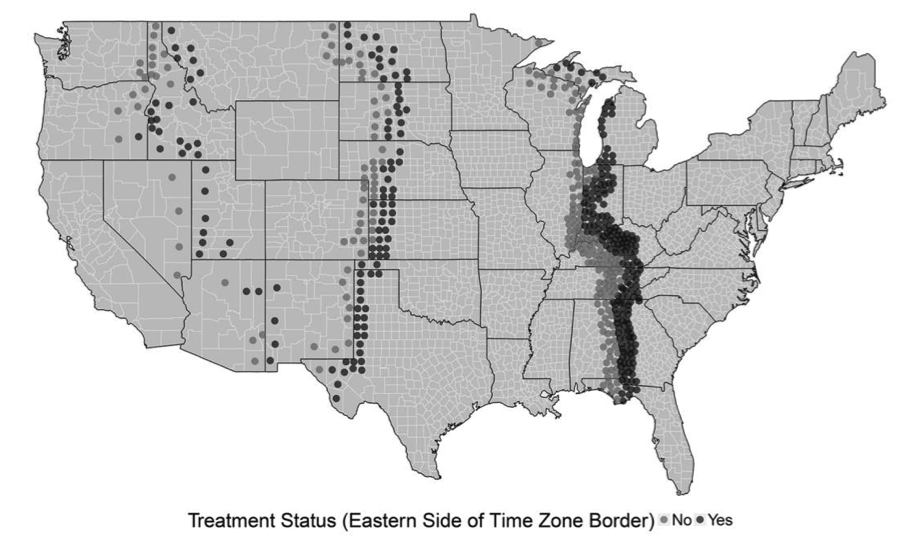
\includegraphics{./imgs/RDD_fig-01.png}

}

\caption{Condados utilizados en la comparación en Schafer y Holbein
(2020)\marginpar{\begin{footnotesize}\leavevmode\vadjust pre{\protect\hypertarget{ref-schafer2020time}{}}%
Schafer, Jerome, y John B Holbein. 2020. {«When time is of the essence:
A natural experiment on how time constraints influence elections»}.
\emph{The Journal of Politics} 82 (2): 418-32.\vspace{2mm}\par\end{footnotesize}}
a uno y otro lado del cambio de huso horario.}

\end{figure}

Esto significa que a un lado y al otro de la zona horaria los condados
son comparables en todas las características observadas y no observadas,
salvo en la zona horaria y el efecto de ella en las restricciones de
tiempo. Es decir, que los condados a un lado y al otro de la frontera
horaria son comparables en todas las características excepto en la hora
local.

Aprovechando esto, los autores estiman el efecto con un modelo de
regresión discontinua\sidenote{\footnotesize Para detalles del ajuste pueden ver el
  código que acompaña a la Figura~\ref{fig-LATE-nolineal}.}. En la
figura siguiente se puede ver cómo se comporta la participación
electoral en función de la distancia a la frontera horaria:

\begin{figure}

{\centering 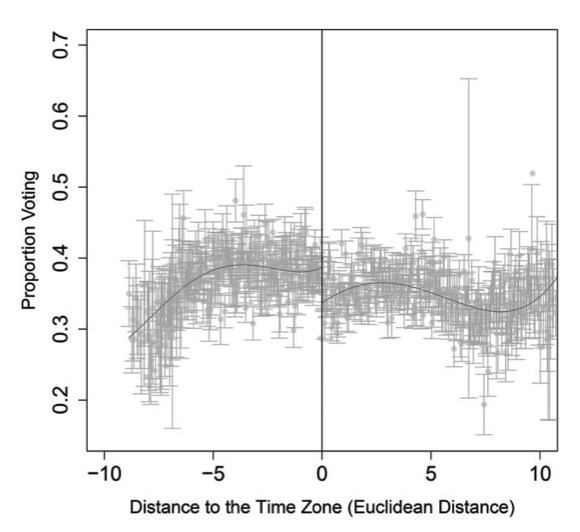
\includegraphics{./imgs/RDD_fig-02.png}

}

\caption{Participación electoral en función de la running variable. El 0
es el cambio de huso horario. La discontinuidad en la distancia cero es
la estimación del efecto causal. Schafer y Holbein
(2020)\marginpar{\begin{footnotesize}\leavevmode\vadjust pre{\protect\hypertarget{ref-schafer2020time}{}}%
Schafer, Jerome, y John B Holbein. 2020. {«When time is of the essence:
A natural experiment on how time constraints influence elections»}.
\emph{The Journal of Politics} 82 (2): 418-32.\vspace{2mm}\par\end{footnotesize}}.}

\end{figure}

Es con estas herramientas que el estudio concluye que los ciudadanos que
viven en el lado inmediatamente oriental de una frontera horaria votan
significativamente menos (entre \(1.5\) y \(3\) puntos porcentuales) que
aquellos en el lado occidental.

\hypertarget{cuxf3mo-se-estima-el-efecto-causal}{%
\section{¿Cómo se estima el efecto
causal?}\label{cuxf3mo-se-estima-el-efecto-causal}}

Si vemos la Figura~\ref{fig-LATE-lm}, podemos ver que la diferencia
entre las dos rectas es el efecto del programa de tutorías. Pero, ¿cómo
se estima? Bueno, la forma más sencilla de hacerlo es ajustar un modelo
lineal a los datos y calcular la diferencia entre las ordenadas al
origen de las rectas ajustadas a cada grupo. Pero esta no es la única
forma de calcular el \textbf{LATE}. En lo que sigue vamos a explorar
variantes de esta estimación y ver cómo afectan en el efecto estimado.

\hypertarget{estimaciuxf3n-paramuxe9trica}{%
\subsection{Estimación paramétrica}\label{estimaciuxf3n-paramuxe9trica}}

Una de las alternativas que tenemos es hacer una estimación paramétrica
o no paramétrica. Pero, ¿a qué nos referimos con esto? En una estimación
paramétrica, como la que vimos en el ejemplo anterior, ajustamos un
modelo a los datos que está definido por parámetros, como podría ser un
modelo lineal.

El primer modelo que vamos a ajustar es el siguiente:

\[
y = \beta_0 + \beta_1 \text{Running variable (centrada)} + \beta_2 \text{indicadora del tratamiento}
\]

Que en nuestro caso sería más bien:

\[
nota_{salida} = \beta_0 + \beta_1 (nota_{entrada}-70) + \beta_2 \mathbb{I}_{tutoria}
\]

donde \(\mathbb{I}_{tutoria}\) es una variable indicadora que toma el
valor de \(1\) si el estudiante participó del programa de tutorías y
\(0\) si no, \(nota_{entrada}\) es la nota del examen de entrada y
\(nota_{salida}\) es la nota del examen de salida. Pero ¿por qué le
restamos \(70\) a la nota de entrada? Bueno, porque queremos centrar la
\emph{running variable} en el umbral. Es decir, queremos que el umbral
sea \(0\) y que los valores a la izquierda del umbral sean negativos y
los valores a la derecha sean positivos. Esto nos va a permitir
interpretar mejor los coeficientes del modelo\sidenote{\footnotesize En realidad, no
  es necesario centrar la \emph{running variable} cuando el ajuste es
  una recta, pero cuando no lo es, queremos que la diferencia en
  ordenadas al origen (cuando la \emph{running variable} vale \(0\)) sea
  el \textbf{LATE}. Igualmente es una buena práctica centrar la
  \emph{running variable}.}.

\begin{Shaded}
\begin{Highlighting}[]
\FunctionTok{modelsummary}\NormalTok{(}\FunctionTok{list}\NormalTok{(}\StringTok{"Lineal"}\OtherTok{=}\NormalTok{ modelo\_lm),}
             \AttributeTok{coef\_rename =} \FunctionTok{c}\NormalTok{(}\StringTok{"entrance\_centered"} \OtherTok{=} \StringTok{"Nota inicial centrada"}\NormalTok{,}
                             \StringTok{"tutoringSí"} \OtherTok{=} \StringTok{"Participó en la tutoría"}\NormalTok{),}
             \AttributeTok{statistic =} \ConstantTok{NULL}\NormalTok{, }
             \AttributeTok{gof\_omit =} \StringTok{".*"}\NormalTok{,}
             \AttributeTok{output =} \StringTok{"gt"}\NormalTok{) }\SpecialCharTok{|\textgreater{}}
  \FunctionTok{gt\_highlight\_rows}\NormalTok{(}\AttributeTok{rows =} \DecValTok{3}\NormalTok{, }
                    \AttributeTok{fill =} \StringTok{"lightyellow"}\NormalTok{,}
                    \AttributeTok{font\_weight =} \StringTok{"bold"}\NormalTok{)}
\end{Highlighting}
\end{Shaded}

\begin{table}
\fontsize{12.0pt}{14.4pt}\selectfont
\begin{tabular*}{\linewidth}{@{\extracolsep{\fill}}lc}
\toprule
  & Lineal \\ 
\midrule\addlinespace[2.5pt]
(Intercept) & 59.411 \\ 
Nota inicial centrada & 0.510 \\ 
{\bfseries \cellcolor[HTML]{rgba(255,255,224,0.8)}{\textcolor[HTML]{000000}{Participó en la tutoría}}} & {\bfseries \cellcolor[HTML]{rgba(255,255,224,0.8)}{\textcolor[HTML]{000000}{10.800}}} \\ 
\bottomrule
\end{tabular*}
\end{table}

Estimaciones del LATE utilizando un modelo lineal.

El coeficiente de la variable indicadora del tratamiento es el
\textbf{LATE}. En este caso, el modelo nos dice que el programa de
tutorías aumenta en 10.8 puntos la nota del examen de salida, en
promedio, para los estudiantes que están cerca del umbral. Si vemos la
Figura~\ref{fig-LATE-lm}, podemos ver que esta estimación tiene sentido.

También podríamos ajustar otro modelo lineal\sidenote{\footnotesize ¿Por qué esto
  sigue siendo un modelo lineal?}, en el que suponemos que la relación
entre la \emph{running variable} y el resultado es cuadrática. No vamos
a escribir el modelo porque se complica un poco ya que ajustamos una
parábola a cada lado de la discontinuidad. Pero la idea es la misma:
ajustamos un modelo lineal a los datos y calculamos la diferencia entre
las estimaciones de los modelos para el umbral (la \emph{running
variable} centrada igual a 0)\sidenote{\footnotesize Para detalles del ajuste pueden
  ver el código que acompaña a la Figura~\ref{fig-LATE-nolineal}.}.

\begin{Shaded}
\begin{Highlighting}[]
\NormalTok{tutoring\_centered }\OtherTok{\textless{}{-}}\NormalTok{ tutoring\_centered }\SpecialCharTok{|\textgreater{}} 
  \FunctionTok{mutate}\NormalTok{(}\AttributeTok{entrance\_centered\_2 =}\NormalTok{ entrance\_centered}\SpecialCharTok{\^{}}\DecValTok{2}\NormalTok{,}
         \AttributeTok{entrance\_centered\_3 =}\NormalTok{ entrance\_centered}\SpecialCharTok{\^{}}\DecValTok{3}\NormalTok{)}

\NormalTok{modelo\_sq\_1 }\OtherTok{\textless{}{-}} \FunctionTok{lm}\NormalTok{(exit\_exam }\SpecialCharTok{\textasciitilde{}}\NormalTok{ entrance\_centered\_2, }
                  \AttributeTok{data =}\NormalTok{ tutoring\_centered }\SpecialCharTok{\%\textgreater{}\%}
                    \FunctionTok{filter}\NormalTok{(entrance\_centered }\SpecialCharTok{\textless{}=} \DecValTok{0}\NormalTok{))}

\NormalTok{modelo\_sq\_2 }\OtherTok{\textless{}{-}} \FunctionTok{lm}\NormalTok{(exit\_exam }\SpecialCharTok{\textasciitilde{}}\NormalTok{ entrance\_centered\_2,}
                  \AttributeTok{data =}\NormalTok{ tutoring\_centered }\SpecialCharTok{\%\textgreater{}\%}
                    \FunctionTok{filter}\NormalTok{(entrance\_centered }\SpecialCharTok{\textgreater{}} \DecValTok{0}\NormalTok{))}

\NormalTok{modelo\_cub\_1 }\OtherTok{\textless{}{-}} \FunctionTok{lm}\NormalTok{(exit\_exam }\SpecialCharTok{\textasciitilde{}}\NormalTok{ entrance\_centered\_3, }
                  \AttributeTok{data =}\NormalTok{ tutoring\_centered }\SpecialCharTok{\%\textgreater{}\%}
                    \FunctionTok{filter}\NormalTok{(entrance\_centered }\SpecialCharTok{\textless{}=} \DecValTok{0}\NormalTok{))}

\NormalTok{modelo\_cub\_2 }\OtherTok{\textless{}{-}} \FunctionTok{lm}\NormalTok{(exit\_exam }\SpecialCharTok{\textasciitilde{}}\NormalTok{ entrance\_centered\_3,}
                  \AttributeTok{data =}\NormalTok{ tutoring\_centered }\SpecialCharTok{\%\textgreater{}\%}
                    \FunctionTok{filter}\NormalTok{(entrance\_centered }\SpecialCharTok{\textgreater{}} \DecValTok{0}\NormalTok{))}

\NormalTok{tutoring\_centered }\OtherTok{\textless{}{-}}\NormalTok{ tutoring\_centered }\SpecialCharTok{\%\textgreater{}\%}
  \FunctionTok{add\_predictions}\NormalTok{(modelo\_lm, }\AttributeTok{var =} \StringTok{"exit\_pred\_lm"}\NormalTok{) }\SpecialCharTok{\%\textgreater{}\%}
  \FunctionTok{add\_predictions}\NormalTok{(modelo\_sq\_1, }\AttributeTok{var =} \StringTok{"exit\_pred\_sq1"}\NormalTok{) }\SpecialCharTok{\%\textgreater{}\%}
  \FunctionTok{add\_predictions}\NormalTok{(modelo\_sq\_2, }\AttributeTok{var =} \StringTok{"exit\_pred\_sq2"}\NormalTok{) }\SpecialCharTok{\%\textgreater{}\%}
  \FunctionTok{add\_predictions}\NormalTok{(modelo\_cub\_1, }\AttributeTok{var =} \StringTok{"exit\_pred\_cub1"}\NormalTok{) }\SpecialCharTok{\%\textgreater{}\%}
  \FunctionTok{add\_predictions}\NormalTok{(modelo\_cub\_2, }\AttributeTok{var =} \StringTok{"exit\_pred\_cub2"}\NormalTok{)}

\NormalTok{colors }\OtherTok{\textless{}{-}} \FunctionTok{c}\NormalTok{(}\StringTok{"Lineal"} \OtherTok{=} \StringTok{"darkgreen"}\NormalTok{, }
            \StringTok{"Cuadrático"} \OtherTok{=} \StringTok{"darkred"}\NormalTok{, }
            \StringTok{"Cúbico"} \OtherTok{=} \StringTok{"darkorange"}\NormalTok{)}

\FunctionTok{ggplot}\NormalTok{(tutoring\_centered, }\FunctionTok{aes}\NormalTok{(}\AttributeTok{x =}\NormalTok{ entrance\_centered, }
                     \AttributeTok{y =}\NormalTok{ exit\_exam)) }\SpecialCharTok{+}
  \FunctionTok{geom\_point}\NormalTok{(}\AttributeTok{size =} \FloatTok{1.5}\NormalTok{, }\AttributeTok{alpha =}\NormalTok{ .}\DecValTok{2}\NormalTok{) }\SpecialCharTok{+} 
  \CommentTok{\# Agregamos una linea basada en un modelo lineal para la running variable centrada menor a 0}
  \FunctionTok{geom\_line}\NormalTok{(}\FunctionTok{aes}\NormalTok{(}\AttributeTok{y =}\NormalTok{ exit\_pred\_lm, }\AttributeTok{color =} \StringTok{"Lineal"}\NormalTok{), }\AttributeTok{linewidth =} \DecValTok{1}\NormalTok{) }\SpecialCharTok{+}
  \CommentTok{\# Agregamos una linea basada en un modelo lineal para la running variable centrada al cuadrado menor a 0}
  \FunctionTok{geom\_line}\NormalTok{(}\AttributeTok{data =} \FunctionTok{filter}\NormalTok{(tutoring\_centered, entrance\_centered }\SpecialCharTok{\textless{}=} \DecValTok{0}\NormalTok{), }\FunctionTok{aes}\NormalTok{(}\AttributeTok{y =}\NormalTok{ exit\_pred\_sq1, }\AttributeTok{color =} \StringTok{"Cuadrático"}\NormalTok{), }
            \AttributeTok{linewidth =} \DecValTok{1}\NormalTok{) }\SpecialCharTok{+}
  \CommentTok{\# Agregamos una linea basada en un modelo lineal para la running variable centrada al cuadrado mayor a 0}
  \FunctionTok{geom\_line}\NormalTok{(}\AttributeTok{data =} \FunctionTok{filter}\NormalTok{(tutoring\_centered, entrance\_centered }\SpecialCharTok{\textgreater{}} \DecValTok{0}\NormalTok{), }\FunctionTok{aes}\NormalTok{(}\AttributeTok{y =}\NormalTok{ exit\_pred\_sq2, }\AttributeTok{color =} \StringTok{"Cuadrático"}\NormalTok{), }
            \AttributeTok{linewidth =} \DecValTok{1}\NormalTok{) }\SpecialCharTok{+}
    \CommentTok{\# Agregamos una linea basada en un modelo lineal para la running variable centrada al cubo menor a 0}
  \FunctionTok{geom\_line}\NormalTok{(}\AttributeTok{data =} \FunctionTok{filter}\NormalTok{(tutoring\_centered, entrance\_centered }\SpecialCharTok{\textless{}=} \DecValTok{0}\NormalTok{), }\FunctionTok{aes}\NormalTok{(}\AttributeTok{y =}\NormalTok{ exit\_pred\_cub1, }\AttributeTok{color =} \StringTok{"Cúbico"}\NormalTok{), }
            \AttributeTok{linewidth =} \DecValTok{1}\NormalTok{) }\SpecialCharTok{+}
  \CommentTok{\# Agregamos una linea basada en un modelo lineal para la running variable centrada al cubo mayor a 0}
  \FunctionTok{geom\_line}\NormalTok{(}\AttributeTok{data =} \FunctionTok{filter}\NormalTok{(tutoring\_centered, entrance\_centered }\SpecialCharTok{\textgreater{}} \DecValTok{0}\NormalTok{), }\FunctionTok{aes}\NormalTok{(}\AttributeTok{y =}\NormalTok{ exit\_pred\_cub2, }\AttributeTok{color =} \StringTok{"Cúbico"}\NormalTok{), }
            \AttributeTok{linewidth =} \DecValTok{1}\NormalTok{) }\SpecialCharTok{+}
  \CommentTok{\# Ponemos una línea vertical en el umbral}
  \FunctionTok{geom\_vline}\NormalTok{(}\AttributeTok{xintercept =} \DecValTok{0}\NormalTok{, }\AttributeTok{color =} \StringTok{"steelblue"}\NormalTok{, }\AttributeTok{linetype =} \StringTok{"dashed"}\NormalTok{) }\SpecialCharTok{+} 
  \CommentTok{\# Las lables}
  \FunctionTok{labs}\NormalTok{(}\AttributeTok{x =} \StringTok{"Puntaje en el examen de entrada (centrado)"}\NormalTok{, }
       \AttributeTok{y =} \StringTok{"Puntaje en el examen de salida"}\NormalTok{,}
       \AttributeTok{color =} \ConstantTok{NULL}\NormalTok{,}
       \AttributeTok{fill =} \StringTok{"Participó en la tutoría"}\NormalTok{) }\SpecialCharTok{+} 
  \CommentTok{\# Colores más chetos}
  \FunctionTok{scale\_color\_manual}\NormalTok{(}\AttributeTok{values =}\NormalTok{ colors) }\SpecialCharTok{+}
  \CommentTok{\#scale\_color\_brewer(palette = "Dark2") +}
  \FunctionTok{scale\_fill\_brewer}\NormalTok{(}\AttributeTok{palette =} \StringTok{"Dark2"}\NormalTok{) }\SpecialCharTok{+}
  \CommentTok{\# Theme sin fondo gris}
  \FunctionTok{theme\_minimal}\NormalTok{() }\SpecialCharTok{+}
  \FunctionTok{theme}\NormalTok{(}\AttributeTok{legend.position =} \StringTok{"top"}\NormalTok{)}
\CommentTok{\#\textgreater{} Ignoring unknown labels:}
\CommentTok{\#\textgreater{} * fill : "Participó en la tutoría"}
\end{Highlighting}
\end{Shaded}

\begin{figure}[H]

{\centering 
\includegraphics[width=18.75in,height=\textheight]{./reg_discontinua_files/figure-pdf/fig-LATE-nolineal-1.pdf}

}

\caption{\label{fig-LATE-nolineal}Notas de entrada vs.~notas de salida
con ajuste lineal, cuadrático y cúbico para cada grupo.}

\end{figure}

Como vemos en la Figura~\ref{fig-LATE-nolineal}, depende cómo ajustemos
el modelo, el efecto del programa de tutorías cambia. En este caso, el
ajuste lineal nos da un efecto de 3.6, el cuadrático de 5.7 y el cúbico
de 3.6. Es decir, la elección de cómo ajustamos a los datos a cada lado
del umbral afecta mi \textbf{LATE}.

Entonces: ¿Cómo decidimos qué ajuste usar? Esto, como vamos a ver más
adelante no tiene una respuesta concreta, hay que ver los datos y, más
importante aún, ver cuán sensibles son nuestros resultados a estas
elecciones. Por ejemplo, si al pasar de una recta a una parábola el
efecto pasa de \(100\) a \(0\), entonces es probable que la elección de
la forma de ajuste sea importante y debamos justificarla. Si, por el
contrario, el efecto no cambia mucho, entonces podemos estar más
tranquilos.

\begin{Shaded}
\begin{Highlighting}[]
\CommentTok{\# Armo una tabla con los valores de los ajustes}
\NormalTok{tutoring\_centered }\SpecialCharTok{\%\textgreater{}\%}
  \FunctionTok{summarise}\NormalTok{(}\StringTok{"Lineal"} \OtherTok{=} \FunctionTok{round}\NormalTok{(}\FunctionTok{predict}\NormalTok{(modelo\_lm, }\AttributeTok{newdata =} \FunctionTok{tibble}\NormalTok{(}\AttributeTok{entrance\_centered =} \DecValTok{0}\NormalTok{, }\AttributeTok{tutoring =} \StringTok{"Sí"}\NormalTok{)) }\SpecialCharTok{{-}} \FunctionTok{predict}\NormalTok{(modelo\_lm, }\AttributeTok{newdata =} \FunctionTok{tibble}\NormalTok{(}\AttributeTok{entrance\_centered =} \DecValTok{0}\NormalTok{, }\AttributeTok{tutoring =} \StringTok{"No"}\NormalTok{)), }\DecValTok{1}\NormalTok{),}
            \StringTok{"Cuadrático"} \OtherTok{=} \FunctionTok{round}\NormalTok{(}\FunctionTok{predict}\NormalTok{(modelo\_sq\_1, }\AttributeTok{newdata =} \FunctionTok{tibble}\NormalTok{(}\AttributeTok{entrance\_centered\_2 =} \DecValTok{0}\NormalTok{)) }\SpecialCharTok{{-}} 
                                   \FunctionTok{predict}\NormalTok{(modelo\_sq\_2, }\AttributeTok{newdata =} \FunctionTok{tibble}\NormalTok{(}\AttributeTok{entrance\_centered\_2 =} \DecValTok{0}\NormalTok{)), }\DecValTok{1}\NormalTok{),}
            \StringTok{"Cúbico"} \OtherTok{=} \FunctionTok{round}\NormalTok{(}\FunctionTok{predict}\NormalTok{(modelo\_cub\_1, }\AttributeTok{newdata =} \FunctionTok{tibble}\NormalTok{(}\AttributeTok{entrance\_centered\_3 =} \DecValTok{0}\NormalTok{)) }\SpecialCharTok{{-}} 
                               \FunctionTok{predict}\NormalTok{(modelo\_cub\_2, }\AttributeTok{newdata =} \FunctionTok{tibble}\NormalTok{(}\AttributeTok{entrance\_centered\_3 =} \DecValTok{0}\NormalTok{)), }\DecValTok{1}\NormalTok{)) }\SpecialCharTok{\%\textgreater{}\%}
  \FunctionTok{pivot\_longer}\NormalTok{(}\FunctionTok{everything}\NormalTok{(), }\AttributeTok{names\_to =} \StringTok{"Modelo"}\NormalTok{, }\AttributeTok{values\_to =} \StringTok{"LATE"}\NormalTok{) }\SpecialCharTok{\%\textgreater{}\%}
  \FunctionTok{gt}\NormalTok{() }\SpecialCharTok{|\textgreater{}}
  \FunctionTok{tab\_header}\NormalTok{(}\AttributeTok{title =} \StringTok{"Estimaciones del LATE para distintos ajustes"}\NormalTok{) }\SpecialCharTok{\%\textgreater{}\%}
  \FunctionTok{fmt\_number}\NormalTok{(}\AttributeTok{columns =} \FunctionTok{vars}\NormalTok{(LATE), }\AttributeTok{decimals =} \DecValTok{1}\NormalTok{) }\SpecialCharTok{\%\textgreater{}\%}
  \FunctionTok{gt\_highlight\_cols}\NormalTok{(}\AttributeTok{columns =} \DecValTok{2}\NormalTok{, }
                    \AttributeTok{fill =} \StringTok{"lightyellow"}\NormalTok{,}
                    \AttributeTok{font\_weight =} \StringTok{"bold"}\NormalTok{)}
\CommentTok{\#\textgreater{} Warning: Since gt v0.3.0, \textasciigrave{}columns = vars(...)\textasciigrave{} has been deprecated.}
\CommentTok{\#\textgreater{} * Please use \textasciigrave{}columns = c(...)\textasciigrave{} instead.}
\end{Highlighting}
\end{Shaded}

\begin{table}
\caption*{
{\large Estimaciones del LATE para distintos ajustes}
} 
\fontsize{12.0pt}{14.4pt}\selectfont
\begin{tabular*}{\linewidth}{@{\extracolsep{\fill}}lr}
\toprule
Modelo & LATE \\ 
\midrule\addlinespace[2.5pt]
Lineal & {\bfseries \cellcolor[HTML]{FFFFE0}{\textcolor[HTML]{000000}{10.8}}} \\ 
Cuadrático & {\bfseries \cellcolor[HTML]{FFFFE0}{\textcolor[HTML]{000000}{5.7}}} \\ 
Cúbico & {\bfseries \cellcolor[HTML]{FFFFE0}{\textcolor[HTML]{000000}{3.6}}} \\ 
\bottomrule
\end{tabular*}
\end{table}

Tabla con las estimaciones de los distintos ajustes.

\hypertarget{ancho-de-banda}{%
\subsection{Ancho de banda}\label{ancho-de-banda}}

Volvamos a la idea de por qué usamos todos los datos si en realidad
queremos comparar a un lado y otro del umbral. Bueno, una forma de
lidiar con esto es limitar el análisis a un cierto rango de la
\emph{running variable}. Es decir, podemos decidir que sólo vamos a
comparar a los estudiantes que están dentro de un cierto rango del
umbral. Por ejemplo, podríamos decidir que sólo vamos a comparar a los
estudiantes que están entre \(65\) y \(75\) puntos en el examen de
entrada. Esto se conoce como \textbf{ancho de banda} y es una forma de
limitar el análisis a los estudiantes que están más cerca del umbral.

Repitamos el ajuste lineal de los estudiantes de cada lado del umbral
pero limitando el ancho de banda. Primero con ancho de banda total,
luego con ancho de banda de \(10\) punto (es decir, sólo analizando los
datos entre \(60\) y \(80\) puntos) y finalmente con un ancho de banda
de \(5\) puntos (es decir, sólo analizando los datos entre \(65\) y
\(75\) puntos).

\begin{Shaded}
\begin{Highlighting}[]
\CommentTok{\# Ahora probemos bajando el bandwidth}
\CommentTok{\# BW = 10}
\NormalTok{model\_bw\_10 }\OtherTok{\textless{}{-}} \FunctionTok{lm}\NormalTok{(exit\_exam }\SpecialCharTok{\textasciitilde{}}\NormalTok{ entrance\_centered }\SpecialCharTok{+}\NormalTok{ tutoring,}
                  \AttributeTok{data =} \FunctionTok{filter}\NormalTok{(tutoring\_centered,}
\NormalTok{                                entrance\_centered }\SpecialCharTok{\textgreater{}=} \SpecialCharTok{{-}}\DecValTok{10} \SpecialCharTok{\&} 
\NormalTok{                                  entrance\_centered }\SpecialCharTok{\textless{}=} \DecValTok{10}\NormalTok{))}
\FunctionTok{tidy}\NormalTok{(model\_bw\_10)}
\CommentTok{\#\textgreater{} \# A tibble: 3 x 5}
\CommentTok{\#\textgreater{}   term              estimate std.error statistic   p.value}
\CommentTok{\#\textgreater{}   \textless{}chr\textgreater{}                \textless{}dbl\textgreater{}     \textless{}dbl\textgreater{}     \textless{}dbl\textgreater{}     \textless{}dbl\textgreater{}}
\CommentTok{\#\textgreater{} 1 (Intercept)         60.4       0.752     80.3  2.99e{-}249}
\CommentTok{\#\textgreater{} 2 entrance\_centered    0.388     0.114      3.40 7.45e{-}  4}
\CommentTok{\#\textgreater{} 3 tutoringSí           9.27      1.31       7.09 6.27e{-} 12}

\CommentTok{\# BW = 5}
\NormalTok{model\_bw\_5 }\OtherTok{\textless{}{-}} \FunctionTok{lm}\NormalTok{(exit\_exam }\SpecialCharTok{\textasciitilde{}}\NormalTok{ entrance\_centered }\SpecialCharTok{+}\NormalTok{ tutoring,}
                 \AttributeTok{data =} \FunctionTok{filter}\NormalTok{(tutoring\_centered,}
\NormalTok{                               entrance\_centered }\SpecialCharTok{\textgreater{}=} \SpecialCharTok{{-}}\DecValTok{5} \SpecialCharTok{\&} 
\NormalTok{                                 entrance\_centered }\SpecialCharTok{\textless{}=} \DecValTok{5}\NormalTok{))}
\FunctionTok{tidy}\NormalTok{(model\_bw\_5)}
\CommentTok{\#\textgreater{} \# A tibble: 3 x 5}
\CommentTok{\#\textgreater{}   term              estimate std.error statistic   p.value}
\CommentTok{\#\textgreater{}   \textless{}chr\textgreater{}                \textless{}dbl\textgreater{}     \textless{}dbl\textgreater{}     \textless{}dbl\textgreater{}     \textless{}dbl\textgreater{}}
\CommentTok{\#\textgreater{} 1 (Intercept)         60.6       1.12      54.3  4.78e{-}118}
\CommentTok{\#\textgreater{} 2 entrance\_centered    0.380     0.331      1.15 2.53e{-}  1}
\CommentTok{\#\textgreater{} 3 tutoringSí           9.12      1.91       4.77 3.66e{-}  6}

\CommentTok{\# Veamos el ajuste de cada uno de estos modelos}
\CommentTok{\# Full BW}
\NormalTok{p\_full }\OtherTok{\textless{}{-}} \FunctionTok{ggplot}\NormalTok{(tutoring, }\FunctionTok{aes}\NormalTok{(}\AttributeTok{x =}\NormalTok{ entrance\_exam, }
                               \AttributeTok{y =}\NormalTok{ exit\_exam, }
                               \AttributeTok{color =}\NormalTok{ tutoring,}
                               \AttributeTok{fill =}\NormalTok{ tutoring)) }\SpecialCharTok{+}
  \FunctionTok{geom\_point}\NormalTok{(}\AttributeTok{size =} \FloatTok{1.5}\NormalTok{, }\AttributeTok{alpha =} \FloatTok{0.5}\NormalTok{) }\SpecialCharTok{+} 
  \CommentTok{\# Add a line based on a linear model for the people scoring 70 or less}
  \FunctionTok{geom\_segment}\NormalTok{(}\AttributeTok{x =} \FunctionTok{min}\NormalTok{(tutoring}\SpecialCharTok{$}\NormalTok{entrance\_exam), }\AttributeTok{xend =} \DecValTok{70}\NormalTok{,}
               \AttributeTok{y =}\NormalTok{ modelo\_lm}\SpecialCharTok{$}\NormalTok{coefficients[}\DecValTok{1}\NormalTok{]}\SpecialCharTok{+}\FunctionTok{min}\NormalTok{(tutoring\_centered}\SpecialCharTok{$}\NormalTok{entrance\_centered)}\SpecialCharTok{*}\NormalTok{modelo\_lm}\SpecialCharTok{$}\NormalTok{coefficients[}\DecValTok{2}\NormalTok{] }\SpecialCharTok{+}
\NormalTok{                 modelo\_lm}\SpecialCharTok{$}\NormalTok{coefficients[}\DecValTok{3}\NormalTok{],}
               \AttributeTok{yend =}\NormalTok{ modelo\_lm}\SpecialCharTok{$}\NormalTok{coefficients[}\DecValTok{1}\NormalTok{] }\SpecialCharTok{+}\NormalTok{ modelo\_lm}\SpecialCharTok{$}\NormalTok{coefficients[}\DecValTok{3}\NormalTok{],}
               \AttributeTok{color =} \StringTok{"gray30"}\NormalTok{, }\AttributeTok{linewidth =} \DecValTok{1}\NormalTok{) }\SpecialCharTok{+}
  \CommentTok{\# Add a line based on a linear model for the people scoring more than 70}
  \FunctionTok{geom\_segment}\NormalTok{(}\AttributeTok{x =} \DecValTok{70}\NormalTok{, }\AttributeTok{xend =} \FunctionTok{max}\NormalTok{(tutoring}\SpecialCharTok{$}\NormalTok{entrance\_exam),}
               \AttributeTok{y =}\NormalTok{ modelo\_lm}\SpecialCharTok{$}\NormalTok{coefficients[}\DecValTok{1}\NormalTok{],}
               \AttributeTok{yend =}\NormalTok{ modelo\_lm}\SpecialCharTok{$}\NormalTok{coefficients[}\DecValTok{1}\NormalTok{] }\SpecialCharTok{+}\NormalTok{ modelo\_lm}\SpecialCharTok{$}\NormalTok{coefficients[}\DecValTok{2}\NormalTok{]}\SpecialCharTok{*}\FunctionTok{max}\NormalTok{(tutoring\_centered}\SpecialCharTok{$}\NormalTok{entrance\_centered),}
               \AttributeTok{color =} \StringTok{"gray30"}\NormalTok{, }\AttributeTok{linewidth =} \DecValTok{1}\NormalTok{) }\SpecialCharTok{+}
  \CommentTok{\# Ponemos una línea vertical en el umbral}
  \FunctionTok{geom\_vline}\NormalTok{(}\AttributeTok{xintercept =} \DecValTok{70}\NormalTok{, }\AttributeTok{color =} \StringTok{"darkblue"}\NormalTok{, }\AttributeTok{linetype =} \StringTok{"dashed"}\NormalTok{) }\SpecialCharTok{+} 
  \CommentTok{\# Las labels}
  \FunctionTok{labs}\NormalTok{(}\AttributeTok{x =} \ConstantTok{NULL}\NormalTok{, }
       \AttributeTok{y =} \ConstantTok{NULL}\NormalTok{,}
       \AttributeTok{color =} \StringTok{"Participó en la tutoría"}\NormalTok{,}
       \AttributeTok{fill =} \StringTok{"Participó en la tutoría"}\NormalTok{) }\SpecialCharTok{+} 
  \CommentTok{\# Colores más chetos}
  \FunctionTok{scale\_color\_brewer}\NormalTok{(}\AttributeTok{palette =} \StringTok{"Dark2"}\NormalTok{) }\SpecialCharTok{+}
  \FunctionTok{scale\_fill\_brewer}\NormalTok{(}\AttributeTok{palette =} \StringTok{"Dark2"}\NormalTok{) }\SpecialCharTok{+}
  \CommentTok{\# Theme sin fondo gris}
  \FunctionTok{theme\_minimal}\NormalTok{() }\SpecialCharTok{+}
  \FunctionTok{theme}\NormalTok{(}\AttributeTok{legend.position =} \StringTok{"none"}\NormalTok{)}


\CommentTok{\# BW = 10}
\NormalTok{p\_bw10 }\OtherTok{\textless{}{-}}\NormalTok{ tutoring\_centered }\SpecialCharTok{|\textgreater{}}
\NormalTok{  dplyr}\SpecialCharTok{::}\FunctionTok{filter}\NormalTok{(}\FunctionTok{between}\NormalTok{(entrance\_centered, }\SpecialCharTok{{-}}\DecValTok{10}\NormalTok{, }\DecValTok{10}\NormalTok{)) }\SpecialCharTok{|\textgreater{}}
  \FunctionTok{ggplot}\NormalTok{(}\FunctionTok{aes}\NormalTok{(}\AttributeTok{x =}\NormalTok{ entrance\_exam, }
             \AttributeTok{y =}\NormalTok{ exit\_exam, }
             \AttributeTok{color =}\NormalTok{ tutoring,}
             \AttributeTok{fill =}\NormalTok{ tutoring)) }\SpecialCharTok{+}
  \FunctionTok{geom\_point}\NormalTok{(}\AttributeTok{size =} \FloatTok{1.5}\NormalTok{, }\AttributeTok{alpha =} \FloatTok{0.5}\NormalTok{) }\SpecialCharTok{+} 
  \FunctionTok{geom\_point}\NormalTok{(}\AttributeTok{data =}\NormalTok{ tutoring\_centered }\SpecialCharTok{|\textgreater{}}
\NormalTok{               dplyr}\SpecialCharTok{::}\FunctionTok{filter}\NormalTok{(}\SpecialCharTok{!}\FunctionTok{between}\NormalTok{(entrance\_centered, }\SpecialCharTok{{-}}\DecValTok{10}\NormalTok{, }\DecValTok{10}\NormalTok{)), }
             \AttributeTok{size =} \FloatTok{1.5}\NormalTok{, }\AttributeTok{alpha =} \FloatTok{0.3}\NormalTok{, }\AttributeTok{color =} \StringTok{"gray"}\NormalTok{) }\SpecialCharTok{+} 
  \CommentTok{\# Add a line based on a linear model for the people scoring 70 or less}
  \FunctionTok{geom\_segment}\NormalTok{(}\AttributeTok{x =} \DecValTok{60}\NormalTok{, }\AttributeTok{xend =} \DecValTok{70}\NormalTok{,}
               \AttributeTok{y =}\NormalTok{ model\_bw\_10}\SpecialCharTok{$}\NormalTok{coefficients[}\DecValTok{1}\NormalTok{]}\SpecialCharTok{{-}}\DecValTok{10}\SpecialCharTok{*}\NormalTok{model\_bw\_10}\SpecialCharTok{$}\NormalTok{coefficients[}\DecValTok{2}\NormalTok{] }\SpecialCharTok{+}
\NormalTok{                 model\_bw\_10}\SpecialCharTok{$}\NormalTok{coefficients[}\DecValTok{3}\NormalTok{],}
               \AttributeTok{yend =}\NormalTok{ model\_bw\_10}\SpecialCharTok{$}\NormalTok{coefficients[}\DecValTok{1}\NormalTok{] }\SpecialCharTok{+}\NormalTok{ model\_bw\_10}\SpecialCharTok{$}\NormalTok{coefficients[}\DecValTok{3}\NormalTok{],}
               \AttributeTok{color =} \StringTok{"gray30"}\NormalTok{, }\AttributeTok{linewidth =} \DecValTok{1}\NormalTok{) }\SpecialCharTok{+}
  \CommentTok{\# Add a line based on a linear model for the people scoring more than 70}
  \FunctionTok{geom\_segment}\NormalTok{(}\AttributeTok{x =} \DecValTok{70}\NormalTok{, }\AttributeTok{xend =} \DecValTok{80}\NormalTok{,}
               \AttributeTok{y =}\NormalTok{ model\_bw\_10}\SpecialCharTok{$}\NormalTok{coefficients[}\DecValTok{1}\NormalTok{],}
               \AttributeTok{yend =}\NormalTok{ model\_bw\_10}\SpecialCharTok{$}\NormalTok{coefficients[}\DecValTok{1}\NormalTok{] }\SpecialCharTok{+}\NormalTok{ model\_bw\_10}\SpecialCharTok{$}\NormalTok{coefficients[}\DecValTok{2}\NormalTok{]}\SpecialCharTok{*}\DecValTok{10}\NormalTok{,}
               \AttributeTok{color =} \StringTok{"gray30"}\NormalTok{, }\AttributeTok{linewidth =} \DecValTok{1}\NormalTok{) }\SpecialCharTok{+}
  \CommentTok{\# Ponemos una línea vertical en el umbral}
  \FunctionTok{geom\_vline}\NormalTok{(}\AttributeTok{xintercept =} \DecValTok{70}\NormalTok{, }\AttributeTok{color =} \StringTok{"darkblue"}\NormalTok{, }\AttributeTok{linetype =} \StringTok{"dashed"}\NormalTok{) }\SpecialCharTok{+} 
  \CommentTok{\# Las labels}
  \FunctionTok{labs}\NormalTok{(}\AttributeTok{x =} \ConstantTok{NULL}\NormalTok{, }
       \AttributeTok{y =} \StringTok{"Puntaje en el examen de salida"}\NormalTok{,}
       \AttributeTok{color =} \StringTok{"Participó en la tutoría"}\NormalTok{,}
       \AttributeTok{fill =} \StringTok{"Participó en la tutoría"}\NormalTok{) }\SpecialCharTok{+} 
  \CommentTok{\# Colores más chetos}
  \FunctionTok{scale\_color\_brewer}\NormalTok{(}\AttributeTok{palette =} \StringTok{"Dark2"}\NormalTok{) }\SpecialCharTok{+}
  \FunctionTok{scale\_fill\_brewer}\NormalTok{(}\AttributeTok{palette =} \StringTok{"Dark2"}\NormalTok{) }\SpecialCharTok{+}
  \CommentTok{\# Theme sin fondo gris}
  \FunctionTok{theme\_minimal}\NormalTok{() }\SpecialCharTok{+}
  \FunctionTok{theme}\NormalTok{(}\AttributeTok{legend.position =} \StringTok{"none"}\NormalTok{)}

\CommentTok{\# BW = 5}
\NormalTok{p\_bw5 }\OtherTok{\textless{}{-}}\NormalTok{ tutoring\_centered }\SpecialCharTok{|\textgreater{}}
\NormalTok{  dplyr}\SpecialCharTok{::}\FunctionTok{filter}\NormalTok{(}\FunctionTok{between}\NormalTok{(entrance\_centered, }\SpecialCharTok{{-}}\DecValTok{5}\NormalTok{, }\DecValTok{5}\NormalTok{)) }\SpecialCharTok{|\textgreater{}}
  \FunctionTok{ggplot}\NormalTok{(}\FunctionTok{aes}\NormalTok{(}\AttributeTok{x =}\NormalTok{ entrance\_exam, }
             \AttributeTok{y =}\NormalTok{ exit\_exam, }
             \AttributeTok{color =}\NormalTok{ tutoring,}
             \AttributeTok{fill =}\NormalTok{ tutoring)) }\SpecialCharTok{+}
  \FunctionTok{geom\_point}\NormalTok{(}\AttributeTok{size =} \FloatTok{1.5}\NormalTok{, }\AttributeTok{alpha =} \FloatTok{0.5}\NormalTok{) }\SpecialCharTok{+} 
  \FunctionTok{geom\_point}\NormalTok{(}\AttributeTok{data =}\NormalTok{ tutoring\_centered }\SpecialCharTok{|\textgreater{}}
\NormalTok{               dplyr}\SpecialCharTok{::}\FunctionTok{filter}\NormalTok{(}\SpecialCharTok{!}\FunctionTok{between}\NormalTok{(entrance\_centered, }\SpecialCharTok{{-}}\DecValTok{5}\NormalTok{, }\DecValTok{5}\NormalTok{)), }
             \AttributeTok{size =} \FloatTok{1.5}\NormalTok{, }\AttributeTok{alpha =} \FloatTok{0.3}\NormalTok{, }\AttributeTok{color =} \StringTok{"gray"}\NormalTok{) }\SpecialCharTok{+} 
  \CommentTok{\# Add a line based on a linear model for the people scoring 70 or less}
  \FunctionTok{geom\_segment}\NormalTok{(}\AttributeTok{x =} \DecValTok{65}\NormalTok{, }\AttributeTok{xend =} \DecValTok{70}\NormalTok{,}
               \AttributeTok{y =}\NormalTok{ model\_bw\_5}\SpecialCharTok{$}\NormalTok{coefficients[}\DecValTok{1}\NormalTok{]}\SpecialCharTok{{-}}\DecValTok{5}\SpecialCharTok{*}\NormalTok{model\_bw\_5}\SpecialCharTok{$}\NormalTok{coefficients[}\DecValTok{2}\NormalTok{] }\SpecialCharTok{+}
\NormalTok{                 model\_bw\_5}\SpecialCharTok{$}\NormalTok{coefficients[}\DecValTok{3}\NormalTok{],}
               \AttributeTok{yend =}\NormalTok{ model\_bw\_5}\SpecialCharTok{$}\NormalTok{coefficients[}\DecValTok{1}\NormalTok{] }\SpecialCharTok{+}\NormalTok{ model\_bw\_5}\SpecialCharTok{$}\NormalTok{coefficients[}\DecValTok{3}\NormalTok{],}
               \AttributeTok{color =} \StringTok{"gray30"}\NormalTok{, }\AttributeTok{linewidth =} \DecValTok{1}\NormalTok{) }\SpecialCharTok{+}
  \CommentTok{\# Add a line based on a linear model for the people scoring more than 70}
  \FunctionTok{geom\_segment}\NormalTok{(}\AttributeTok{x =} \DecValTok{70}\NormalTok{, }\AttributeTok{xend =} \DecValTok{75}\NormalTok{,}
               \AttributeTok{y =}\NormalTok{ model\_bw\_5}\SpecialCharTok{$}\NormalTok{coefficients[}\DecValTok{1}\NormalTok{],}
               \AttributeTok{yend =}\NormalTok{ model\_bw\_5}\SpecialCharTok{$}\NormalTok{coefficients[}\DecValTok{1}\NormalTok{] }\SpecialCharTok{+}\NormalTok{ model\_bw\_5}\SpecialCharTok{$}\NormalTok{coefficients[}\DecValTok{2}\NormalTok{]}\SpecialCharTok{*}\DecValTok{5}\NormalTok{,}
               \AttributeTok{color =} \StringTok{"gray30"}\NormalTok{, }\AttributeTok{linewidth =} \DecValTok{1}\NormalTok{) }\SpecialCharTok{+}
  \CommentTok{\# Ponemos una línea vertical en el umbral}
  \FunctionTok{geom\_vline}\NormalTok{(}\AttributeTok{xintercept =} \DecValTok{70}\NormalTok{, }\AttributeTok{color =} \StringTok{"darkblue"}\NormalTok{, }\AttributeTok{linetype =} \StringTok{"dashed"}\NormalTok{) }\SpecialCharTok{+} 
  \CommentTok{\# Las labels}
  \FunctionTok{labs}\NormalTok{(}\AttributeTok{x =} \StringTok{"Puntaje en el examen de entrada"}\NormalTok{, }
       \AttributeTok{y =} \ConstantTok{NULL}\NormalTok{,}
       \AttributeTok{color =} \StringTok{"Participó en la tutoría"}\NormalTok{,}
       \AttributeTok{fill =} \StringTok{"Participó en la tutoría"}\NormalTok{) }\SpecialCharTok{+} 
  \CommentTok{\# Colores más chetos}
  \FunctionTok{scale\_color\_brewer}\NormalTok{(}\AttributeTok{palette =} \StringTok{"Dark2"}\NormalTok{) }\SpecialCharTok{+}
  \FunctionTok{scale\_fill\_brewer}\NormalTok{(}\AttributeTok{palette =} \StringTok{"Dark2"}\NormalTok{) }\SpecialCharTok{+}
  \CommentTok{\# Theme sin fondo gris}
  \FunctionTok{theme\_minimal}\NormalTok{() }\SpecialCharTok{+}
  \FunctionTok{theme}\NormalTok{(}\AttributeTok{legend.position =} \StringTok{"none"}\NormalTok{)}

\FunctionTok{library}\NormalTok{(patchwork)}
\NormalTok{p\_full }\SpecialCharTok{/}\NormalTok{ p\_bw10 }\SpecialCharTok{/}\NormalTok{ p\_bw5 }\SpecialCharTok{+} \FunctionTok{plot\_layout}\NormalTok{(}\AttributeTok{guides =} \StringTok{"collect"}\NormalTok{)}
\end{Highlighting}
\end{Shaded}

\begin{figure}[H]

{\centering 
\includegraphics[width=18.75in,height=\textheight]{./reg_discontinua_files/figure-pdf/unnamed-chunk-10-1.pdf}

}

\caption{Estimaciones del LATE utilizando un modelo lineal con distintos
anchos de banda.}

\end{figure}

En la figura vemos que los ajustes son ligeramente distintos, pero no se
llega a ver una difrencia. Qué pasa si vemos las estimaciones del
modelo:

\begin{Shaded}
\begin{Highlighting}[]
\CommentTok{\# Las estimaciones y el sample size}
\FunctionTok{modelsummary}\NormalTok{(}\FunctionTok{list}\NormalTok{(}\StringTok{"Full data"} \OtherTok{=}\NormalTok{ modelo\_lm, }
                  \StringTok{"Bandwidth = 10"} \OtherTok{=}\NormalTok{ model\_bw\_10, }
                  \StringTok{"Bandwidth = 5"} \OtherTok{=}\NormalTok{ model\_bw\_5), }
             \AttributeTok{coef\_rename =} \FunctionTok{c}\NormalTok{(}\StringTok{"entrance\_centered"} \OtherTok{=} \StringTok{"Nota inicial centrada"}\NormalTok{,}
                             \StringTok{"tutoringSí"} \OtherTok{=} \StringTok{"Participó en la tutoría"}\NormalTok{),}
             \AttributeTok{gof\_omit =} \StringTok{\textquotesingle{}DF|Deviance|R2|AIC|BIC|Log.Lik|F|RMSE\textquotesingle{}}\NormalTok{,}
             \AttributeTok{statistic =} \StringTok{"p = \{p.value\}"}\NormalTok{, }
             \AttributeTok{output =} \StringTok{"gt"}\NormalTok{) }\SpecialCharTok{|\textgreater{}}
  \FunctionTok{gt\_highlight\_rows}\NormalTok{(}\AttributeTok{rows =} \DecValTok{5}\NormalTok{, }
                    \AttributeTok{fill =} \StringTok{"lightyellow"}\NormalTok{,}
                    \AttributeTok{font\_weight =} \StringTok{"bold"}\NormalTok{) }\SpecialCharTok{|\textgreater{}}
  \FunctionTok{gt\_highlight\_rows}\NormalTok{(}\AttributeTok{rows =} \DecValTok{7}\NormalTok{, }
                    \AttributeTok{fill =} \StringTok{"lightyellow"}\NormalTok{,}
                    \AttributeTok{font\_weight =} \StringTok{"bold"}\NormalTok{)}
\end{Highlighting}
\end{Shaded}

\begin{table}
\fontsize{12.0pt}{14.4pt}\selectfont
\begin{tabular*}{\linewidth}{@{\extracolsep{\fill}}lccc}
\toprule
  & Full data & Bandwidth = 10 & Bandwidth = 5 \\ 
\midrule\addlinespace[2.5pt]
(Intercept) & 59.411 & 60.377 & 60.631 \\ 
 & p = <0.001 & p = <0.001 & p = <0.001 \\ 
Nota inicial centrada & 0.510 & 0.388 & 0.380 \\ 
 & p = <0.001 & p = <0.001 & p = 0.253 \\ 
{\bfseries \cellcolor[HTML]{rgba(255,255,224,0.8)}{\textcolor[HTML]{000000}{Participó en la tutoría}}} & {\bfseries \cellcolor[HTML]{rgba(255,255,224,0.8)}{\textcolor[HTML]{000000}{10.800}}} & {\bfseries \cellcolor[HTML]{rgba(255,255,224,0.8)}{\textcolor[HTML]{000000}{9.273}}} & {\bfseries \cellcolor[HTML]{rgba(255,255,224,0.8)}{\textcolor[HTML]{000000}{9.122}}} \\ 
{} & {p = <0.001} & {p = <0.001} & {p = <0.001} \\ 
{\bfseries \cellcolor[HTML]{rgba(255,255,224,0.8)}{\textcolor[HTML]{000000}{Num.Obs.}}} & {\bfseries \cellcolor[HTML]{rgba(255,255,224,0.8)}{\textcolor[HTML]{000000}{1000}}} & {\bfseries \cellcolor[HTML]{rgba(255,255,224,0.8)}{\textcolor[HTML]{000000}{404}}} & {\bfseries \cellcolor[HTML]{rgba(255,255,224,0.8)}{\textcolor[HTML]{000000}{194}}} \\ 
\bottomrule
\end{tabular*}
\end{table}

Hay tres cosas que quiero que vean. Primero, que el \textbf{LATE} es
bastante similar en los tres casos pero se ve afectado por el ancho de
banda. Segundo, el ancho de banda afecta el tamaño de la muestra y, por
lo tanto, la potencia estadística. Y tercero, algo de lo que no habíamos
hablado hasta el momento era de la variabilidad de las estimaciones. Por
ejemplo, en este caso que el \textbf{LATE} es un parámetro de un modelo
lineal como los que ya conocemos, podemos utilizar las herramientas
usuales de inferencia estadística (como el p-valor que ven abajo de la
estimación en la tabla) para sacar conclusiones al respecto.

\hypertarget{kernels}{%
\subsection{\texorpdfstring{\emph{Kernels}}{Kernels}}\label{kernels}}

Como vimos, achicar el ancho de banda mejoraría la estimación (porque
estamos considerando a los sujetos más ``parecido'') pero disminuye el
tamaño de muestra efectivo. Una alternativa a esto es conservar el ancho
de banda pero darle más peso a los puntos que están cerca del umbral.
Por ejemplo, podríamos darle más peso a los puntos que están a \(1\)
punto del umbral que a los que están a \(10\) puntos. Esto se hace
utilizando un \textbf{kernel}. Un kernel es una función que asigna un
peso a cada punto en función de su distancia al umbral. Los
\emph{kernels} pueden tener diversas formas, como triangular o
gaussiano\sidenote{\footnotesize Cuando achicamos el ancho de banda en la sección
  anterior podemos considerar como si hubiéramos utilizado un kernel
  rectangular, es decir, que todos los puntos dentro del ancho de banda
  tienen el mismo peso.}.

Dejenme mostrarles la forma de algunos kernels que vamos a probar:

\begin{Shaded}
\begin{Highlighting}[]
\NormalTok{kernels }\OtherTok{\textless{}{-}} \FunctionTok{tibble}\NormalTok{(}\AttributeTok{x =} \FunctionTok{seq}\NormalTok{(}\SpecialCharTok{{-}}\FloatTok{1.5}\NormalTok{, }\FloatTok{1.5}\NormalTok{, }\AttributeTok{length.out =} \DecValTok{200}\NormalTok{)) }\SpecialCharTok{\%\textgreater{}\%}
  \FunctionTok{mutate}\NormalTok{(}\AttributeTok{rectangular =} \FunctionTok{ifelse}\NormalTok{(}\FunctionTok{abs}\NormalTok{(x) }\SpecialCharTok{\textless{}=} \DecValTok{1}\NormalTok{, }\DecValTok{1}\NormalTok{, }\DecValTok{0}\NormalTok{),}
         \AttributeTok{triangular =} \FunctionTok{ifelse}\NormalTok{(}\FunctionTok{abs}\NormalTok{(x) }\SpecialCharTok{\textless{}=} \DecValTok{1}\NormalTok{, }\DecValTok{1} \SpecialCharTok{{-}} \FunctionTok{abs}\NormalTok{(x), }\DecValTok{0}\NormalTok{),}
         \AttributeTok{epanechnikov =} \FunctionTok{ifelse}\NormalTok{(}\FunctionTok{abs}\NormalTok{(x) }\SpecialCharTok{\textless{}=} \DecValTok{1}\NormalTok{, }\FloatTok{0.75} \SpecialCharTok{*}\NormalTok{ (}\DecValTok{1} \SpecialCharTok{{-}}\NormalTok{ x}\SpecialCharTok{\^{}}\DecValTok{2}\NormalTok{), }\DecValTok{0}\NormalTok{))}

\FunctionTok{ggplot}\NormalTok{(kernels, }\FunctionTok{aes}\NormalTok{(}\AttributeTok{x =}\NormalTok{ x)) }\SpecialCharTok{+}
  \FunctionTok{geom\_line}\NormalTok{(}\FunctionTok{aes}\NormalTok{(}\AttributeTok{y =}\NormalTok{ rectangular, }\AttributeTok{color =} \StringTok{"Rectangular"}\NormalTok{), }\AttributeTok{size =} \DecValTok{1}\NormalTok{) }\SpecialCharTok{+}
  \FunctionTok{geom\_line}\NormalTok{(}\FunctionTok{aes}\NormalTok{(}\AttributeTok{y =}\NormalTok{ triangular, }\AttributeTok{color =} \StringTok{"Triangular"}\NormalTok{), }\AttributeTok{size =} \DecValTok{1}\NormalTok{) }\SpecialCharTok{+}
  \FunctionTok{geom\_line}\NormalTok{(}\FunctionTok{aes}\NormalTok{(}\AttributeTok{y =}\NormalTok{ epanechnikov, }\AttributeTok{color =} \StringTok{"Epanechnikov"}\NormalTok{), }\AttributeTok{size =} \DecValTok{1}\NormalTok{) }\SpecialCharTok{+}
  \FunctionTok{labs}\NormalTok{(}\AttributeTok{x =} \StringTok{"Distancia al umbral"}\NormalTok{, }\AttributeTok{y =} \StringTok{"Peso"}\NormalTok{, }\AttributeTok{color =} \ConstantTok{NULL}\NormalTok{) }\SpecialCharTok{+}
  \FunctionTok{scale\_color\_brewer}\NormalTok{(}\AttributeTok{palette =} \StringTok{"Dark2"}\NormalTok{) }\SpecialCharTok{+}
  \FunctionTok{theme\_minimal}\NormalTok{() }\SpecialCharTok{+}
  \FunctionTok{theme}\NormalTok{(}\AttributeTok{legend.position =} \StringTok{"top"}\NormalTok{)}
\CommentTok{\#\textgreater{} Warning: Using \textasciigrave{}size\textasciigrave{} aesthetic for lines was deprecated in ggplot2 3.4.0.}
\CommentTok{\#\textgreater{} i Please use \textasciigrave{}linewidth\textasciigrave{} instead.}
\end{Highlighting}
\end{Shaded}

\begin{figure}[H]

{\centering 
\includegraphics[width=18.75in,height=\textheight]{./reg_discontinua_files/figure-pdf/unnamed-chunk-12-1.pdf}

}

\caption{Kernel rectancular, triangular y Epanechnikov.}

\end{figure}

Podemos ver que cada kernel pesa los puntos de forma distinta. El kernel
rectangular le da el mismo peso a todos los puntos dentro del ancho de
banda, el triangular le da más peso a los puntos que están cerca del
umbral y el Epanechnikov es un poco menos águdo que el triangular.

La elección del kernel, al igual que en el caso del ancho de banda,
afecta la estimación del \textbf{LATE}.

\hypertarget{ajustes-no-paramuxe9tricos}{%
\subsection{Ajustes no paramétricos}\label{ajustes-no-paramuxe9tricos}}

Finalmente, una alternativa bastante usual es la de estimar el
\textbf{LATE} utilizando un ajuste no paramétrico. Esto significa que no
vamos a asumir una forma funcional específica para la relación entre la
\emph{running variable} y el \emph{outcome}. En cambio, vamos a utilizar
técnicas como los \emph{splines} o los \emph{Locally estimated/weighted
scatterplot smoothing (LOESS)} para ajustar una curva a los datos.

Por ejemplo, veamos cómo se ve la estimación del \textbf{LATE} en este
caso.

\begin{Shaded}
\begin{Highlighting}[]
\FunctionTok{ggplot}\NormalTok{(tutoring\_centered, }\FunctionTok{aes}\NormalTok{(}\AttributeTok{x =}\NormalTok{ entrance\_centered, }
                              \AttributeTok{y =}\NormalTok{ exit\_exam, }
                              \AttributeTok{color =}\NormalTok{ tutoring,}
                              \AttributeTok{fill =}\NormalTok{ tutoring)) }\SpecialCharTok{+}
  \FunctionTok{geom\_point}\NormalTok{(}\AttributeTok{size =} \FloatTok{1.5}\NormalTok{, }\AttributeTok{alpha =}\NormalTok{ .}\DecValTok{3}\NormalTok{) }\SpecialCharTok{+} 
  \CommentTok{\# Agregamos una linea basada en un modelo lineal para la running variable menor a 70}
  \FunctionTok{geom\_smooth}\NormalTok{(}\AttributeTok{data =} \FunctionTok{filter}\NormalTok{(tutoring\_centered, tutoring }\SpecialCharTok{==} \StringTok{"Sí"}\NormalTok{)) }\SpecialCharTok{+}
  \CommentTok{\# Agregamos una linea basada en un modelo lineal para la running variable mayor a 70}
  \FunctionTok{geom\_smooth}\NormalTok{(}\AttributeTok{data =} \FunctionTok{filter}\NormalTok{(tutoring\_centered, tutoring }\SpecialCharTok{==} \StringTok{"No"}\NormalTok{)) }\SpecialCharTok{+}
  \CommentTok{\# Ponemos una línea vertical en el umbral}
  \FunctionTok{geom\_vline}\NormalTok{(}\AttributeTok{xintercept =} \DecValTok{0}\NormalTok{, }\AttributeTok{color =} \StringTok{"darkblue"}\NormalTok{, }\AttributeTok{linetype =} \StringTok{"dashed"}\NormalTok{) }\SpecialCharTok{+} 
  \CommentTok{\# Las lables}
  \FunctionTok{labs}\NormalTok{(}\AttributeTok{x =} \StringTok{"Puntaje en el examen de entrada (centrado)"}\NormalTok{, }
       \AttributeTok{y =} \StringTok{"Puntaje en el examen de salida"}\NormalTok{,}
       \AttributeTok{color =} \StringTok{"Participó en la tutoría"}\NormalTok{,}
       \AttributeTok{fill =} \StringTok{"Participó en la tutoría"}\NormalTok{) }\SpecialCharTok{+} 
  \CommentTok{\# Colores más chetos}
  \FunctionTok{scale\_color\_brewer}\NormalTok{(}\AttributeTok{palette =} \StringTok{"Dark2"}\NormalTok{) }\SpecialCharTok{+}
  \FunctionTok{scale\_fill\_brewer}\NormalTok{(}\AttributeTok{palette =} \StringTok{"Dark2"}\NormalTok{) }\SpecialCharTok{+}
  \CommentTok{\# Theme sin fondo gris}
  \FunctionTok{theme\_minimal}\NormalTok{() }\SpecialCharTok{+}
  \FunctionTok{theme}\NormalTok{(}\AttributeTok{legend.position =} \StringTok{"top"}\NormalTok{)}
\CommentTok{\#\textgreater{} \textasciigrave{}geom\_smooth()\textasciigrave{} using method = \textquotesingle{}loess\textquotesingle{} and formula = \textquotesingle{}y \textasciitilde{} x\textquotesingle{}}
\CommentTok{\#\textgreater{} \textasciigrave{}geom\_smooth()\textasciigrave{} using method = \textquotesingle{}loess\textquotesingle{} and formula = \textquotesingle{}y \textasciitilde{} x\textquotesingle{}}
\end{Highlighting}
\end{Shaded}

\begin{figure}[H]

{\centering 
\includegraphics[width=18.75in,height=\textheight]{./reg_discontinua_files/figure-pdf/unnamed-chunk-13-1.pdf}

}

\end{figure}

En este caso estamos usando la función de \emph{regresión local}
\texttt{geom\_smooth()} de \texttt{ggplot2} para ajustar una curva a los
datos. Esta función utiliza un ajuste \emph{LOESS} por defecto, pero
también podemos especificar otros métodos de ajuste. Podemos ver que no
se trata de una curva suave sino más bien de una especie de promedio
móvil pesado que va siguiendo a los puntos.

En la estimación no paramétrica como en la paramétrica vamos a calcular
el \textbf{LATE} como la diferencia entre las estimaciones del modelo de
cada lado del umbral, y como en el caso anterior, la elección del ancho
de banda y del kernel afecta la estimación del \textbf{LATE}.

Acá ya no es tan fácil obtener la estimación del efecto ajustando
modelos lineales así que vamos a hechar mano de un paquete para esto:
\texttt{rdrobust}. Este paquete nos permite ajustar modelos de regresión
discontinua de forma sencilla y rápida, y nos da una serie de opciones
para ajustar el ancho de banda y el kernel. Empecemos utilizando los
valores por defecto.

\begin{Shaded}
\begin{Highlighting}[]
\NormalTok{full }\OtherTok{\textless{}{-}} \FunctionTok{rdrobust}\NormalTok{(}\AttributeTok{y =}\NormalTok{ tutoring}\SpecialCharTok{$}\NormalTok{exit\_exam, }\AttributeTok{x =}\NormalTok{ tutoring}\SpecialCharTok{$}\NormalTok{entrance\_exam, }\AttributeTok{c =} \DecValTok{70}\NormalTok{) }
\CommentTok{\#\textgreater{} Warning in rdrobust(y = tutoring$exit\_exam, x = tutoring$entrance\_exam, :}
\CommentTok{\#\textgreater{} Mass points detected in the running variable.}
\FunctionTok{summary}\NormalTok{(full)}
\CommentTok{\#\textgreater{} Sharp RD estimates using local polynomial regression.}
\CommentTok{\#\textgreater{} }
\CommentTok{\#\textgreater{} Number of Obs.                 1000}
\CommentTok{\#\textgreater{} BW type                       mserd}
\CommentTok{\#\textgreater{} Kernel                   Triangular}
\CommentTok{\#\textgreater{} VCE method                       NN}
\CommentTok{\#\textgreater{} }
\CommentTok{\#\textgreater{} Number of Obs.                  237          763}
\CommentTok{\#\textgreater{} Eff. Number of Obs.             144          256}
\CommentTok{\#\textgreater{} Order est. (p)                    1            1}
\CommentTok{\#\textgreater{} Order bias  (q)                   2            2}
\CommentTok{\#\textgreater{} BW est. (h)                   9.969        9.969}
\CommentTok{\#\textgreater{} BW bias (b)                  14.661       14.661}
\CommentTok{\#\textgreater{} rho (h/b)                     0.680        0.680}
\CommentTok{\#\textgreater{} Unique Obs.                     155          262}
\CommentTok{\#\textgreater{} }
\CommentTok{\#\textgreater{} =============================================================================}
\CommentTok{\#\textgreater{}         Method     Coef. Std. Err.         z     P\textgreater{}|z|      [ 95\% C.I. ]       }
\CommentTok{\#\textgreater{} =============================================================================}
\CommentTok{\#\textgreater{}   Conventional    {-}8.578     1.601    {-}5.359     0.000   [{-}11.715 , {-}5.441]    }
\CommentTok{\#\textgreater{}         Robust         {-}         {-}    {-}4.352     0.000   [{-}12.101 , {-}4.587]    }
\CommentTok{\#\textgreater{} =============================================================================}
\end{Highlighting}
\end{Shaded}

Vemos que hay mucha información, como el kernel (triangular), el ancho
de banda (\(9.969\))\sidenote{\footnotesize La estimación del ancho de banda utiliza
  un algoritmo \emph{data-drive} al que no vamos a entrar en detalle,
  pero que se basa en la idea de que el ancho de banda óptimo es aquel
  que minimiza el error cuadrático medio de la estimación del
  \textbf{LATE}. Si quieren ver más detalles pueden consultar la
  documentación del paquete \texttt{rdrobust}.}, el número de
observaciones, etc. Más interesante, al final podemos ver la estimación
del \textbf{LATE} que en este caso, el \textbf{LATE} es de 8.6 puntos.

Vamos a ver el ajuste qué pinta tiene utilizando la función
\texttt{rdplot()} del mismo paquete. Esta función nos permite visualizar
el ajuste de la regresión discontinua y ver cómo se ve la estimación del
\textbf{LATE}.

\begin{Shaded}
\begin{Highlighting}[]
\FunctionTok{rdplot}\NormalTok{(}\AttributeTok{y =}\NormalTok{ tutoring}\SpecialCharTok{$}\NormalTok{exit\_exam, }\AttributeTok{x =}\NormalTok{ tutoring}\SpecialCharTok{$}\NormalTok{entrance\_exam, }\AttributeTok{c =} \DecValTok{70}\NormalTok{) }
\CommentTok{\#\textgreater{} [1] "Mass points detected in the running variable."}
\end{Highlighting}
\end{Shaded}

\begin{figure}[H]

{\centering 
\includegraphics[width=18.75in,height=\textheight]{./reg_discontinua_files/figure-pdf/unnamed-chunk-15-1.pdf}

}

\caption{Estimación del LATE utilizando un ajuste no paramétrico.}

\end{figure}

¿Cómo cambia esta estimación si duplicamos el ancho de banda?

\begin{Shaded}
\begin{Highlighting}[]
\NormalTok{doble }\OtherTok{\textless{}{-}} \FunctionTok{rdrobust}\NormalTok{(}\AttributeTok{y =}\NormalTok{ tutoring}\SpecialCharTok{$}\NormalTok{exit\_exam, }\AttributeTok{x =}\NormalTok{ tutoring}\SpecialCharTok{$}\NormalTok{entrance\_exam, }\AttributeTok{c =} \DecValTok{70}\NormalTok{, }\AttributeTok{h =} \FloatTok{9.969} \SpecialCharTok{*} \DecValTok{2}\NormalTok{)}
\FunctionTok{rdplot}\NormalTok{(}\AttributeTok{y =}\NormalTok{ tutoring}\SpecialCharTok{$}\NormalTok{exit\_exam, }\AttributeTok{x =}\NormalTok{ tutoring}\SpecialCharTok{$}\NormalTok{entrance\_exam, }\AttributeTok{c =} \DecValTok{70}\NormalTok{, }\AttributeTok{h =} \DecValTok{2}\SpecialCharTok{*}\FloatTok{9.969}\NormalTok{)}
\CommentTok{\#\textgreater{} [1] "Mass points detected in the running variable."}
\end{Highlighting}
\end{Shaded}

\begin{figure}[H]

{\centering 
\includegraphics[width=18.75in,height=\textheight]{./reg_discontinua_files/figure-pdf/unnamed-chunk-16-1.pdf}

}

\caption{Estimación del LATE utilizando un ajuste no paramétrico con el
doble del ancho de banda estimado de los datos.}

\end{figure}

Veamos las estimaciones del \textbf{LATE} para el ancho de banda
completo, el doble y la mitad del ancho de banda estimado.

\begin{Shaded}
\begin{Highlighting}[]
\CommentTok{\# Un approach posible es usar el recomendado, el doble y la mitad}
\NormalTok{mitad }\OtherTok{\textless{}{-}} \FunctionTok{rdrobust}\NormalTok{(}\AttributeTok{y =}\NormalTok{ tutoring}\SpecialCharTok{$}\NormalTok{exit\_exam, }\AttributeTok{x =}\NormalTok{ tutoring}\SpecialCharTok{$}\NormalTok{entrance\_exam, }\AttributeTok{c =} \DecValTok{70}\NormalTok{, }\AttributeTok{h =} \FloatTok{9.969} \SpecialCharTok{*} \FloatTok{0.5}\NormalTok{) }

\FunctionTok{tibble}\NormalTok{(}\AttributeTok{BW =} \FunctionTok{c}\NormalTok{(}\StringTok{"Full = 9.97"}\NormalTok{, }\StringTok{"Doble = 19.94"}\NormalTok{, }\StringTok{"Mitad = 4.99"}\NormalTok{),}
       \AttributeTok{Estimate =} \SpecialCharTok{{-}}\FunctionTok{round}\NormalTok{(}\FunctionTok{c}\NormalTok{(full}\SpecialCharTok{$}\NormalTok{Estimate[}\DecValTok{1}\NormalTok{], doble}\SpecialCharTok{$}\NormalTok{Estimate[}\DecValTok{1}\NormalTok{], mitad}\SpecialCharTok{$}\NormalTok{Estimate[}\DecValTok{1}\NormalTok{]), }\DecValTok{3}\NormalTok{)) }\SpecialCharTok{|\textgreater{}} 
  \FunctionTok{gt}\NormalTok{()}
\end{Highlighting}
\end{Shaded}

\begin{table}
\fontsize{12.0pt}{14.4pt}\selectfont
\begin{tabular*}{\linewidth}{@{\extracolsep{\fill}}lr}
\toprule
BW & Estimate \\ 
\midrule\addlinespace[2.5pt]
Full = 9.97 & 8.578 \\ 
Doble = 19.94 & 9.151 \\ 
Mitad = 4.99 & 8.201 \\ 
\bottomrule
\end{tabular*}
\end{table}

Si bien hay diferencias, podemos ver que la estimación es bastante
consistente, algo que es deseable y que nos indica que, al menos en esa
región, el efecto es relativamente constante.

Algo que podemos modificar también es el kernel utilizado. Cambiemos de
triangular a uniforme y veamos el ajuste.

\begin{Shaded}
\begin{Highlighting}[]
\FunctionTok{rdplot}\NormalTok{(}\AttributeTok{y =}\NormalTok{ tutoring}\SpecialCharTok{$}\NormalTok{exit\_exam, }\AttributeTok{x =}\NormalTok{ tutoring}\SpecialCharTok{$}\NormalTok{entrance\_exam, }\AttributeTok{c =} \DecValTok{70}\NormalTok{, }\AttributeTok{h =} \FloatTok{9.969}\NormalTok{, }\AttributeTok{kernel =} \StringTok{"uniform"}\NormalTok{)}
\CommentTok{\#\textgreater{} [1] "Mass points detected in the running variable."}
\end{Highlighting}
\end{Shaded}

\begin{figure}[H]

{\centering 
\includegraphics[width=18.75in,height=\textheight]{./reg_discontinua_files/figure-pdf/unnamed-chunk-18-1.pdf}

}

\caption{Estimación del LATE utilizando un ajuste no paramétrico con
kernel uniforme.}

\end{figure}

Y veamos cómo esta elección afecta a la estimación del \textbf{LATE}.

\begin{Shaded}
\begin{Highlighting}[]
\NormalTok{triangular }\OtherTok{\textless{}{-}} \FunctionTok{rdrobust}\NormalTok{(}\AttributeTok{y =}\NormalTok{ tutoring}\SpecialCharTok{$}\NormalTok{exit\_exam, }\AttributeTok{x =}\NormalTok{ tutoring}\SpecialCharTok{$}\NormalTok{entrance\_exam, }\AttributeTok{c =} \DecValTok{70}\NormalTok{, }\AttributeTok{kernel =} \StringTok{"triangular"}\NormalTok{)}
\CommentTok{\#\textgreater{} Warning in rdrobust(y = tutoring$exit\_exam, x = tutoring$entrance\_exam, :}
\CommentTok{\#\textgreater{} Mass points detected in the running variable.}
\NormalTok{epanechnikov }\OtherTok{\textless{}{-}} \FunctionTok{rdrobust}\NormalTok{(}\AttributeTok{y =}\NormalTok{ tutoring}\SpecialCharTok{$}\NormalTok{exit\_exam, }\AttributeTok{x =}\NormalTok{ tutoring}\SpecialCharTok{$}\NormalTok{entrance\_exam, }\AttributeTok{c =} \DecValTok{70}\NormalTok{, }\AttributeTok{kernel =} \StringTok{"epanechnikov"}\NormalTok{)}
\CommentTok{\#\textgreater{} Warning in rdrobust(y = tutoring$exit\_exam, x = tutoring$entrance\_exam, :}
\CommentTok{\#\textgreater{} Mass points detected in the running variable.}
\NormalTok{uniforme }\OtherTok{\textless{}{-}} \FunctionTok{rdrobust}\NormalTok{(}\AttributeTok{y =}\NormalTok{ tutoring}\SpecialCharTok{$}\NormalTok{exit\_exam, }\AttributeTok{x =}\NormalTok{ tutoring}\SpecialCharTok{$}\NormalTok{entrance\_exam, }\AttributeTok{c =} \DecValTok{70}\NormalTok{, }\AttributeTok{kernel =} \StringTok{"uniform"}\NormalTok{)}
\CommentTok{\#\textgreater{} Warning in rdrobust(y = tutoring$exit\_exam, x = tutoring$entrance\_exam, :}
\CommentTok{\#\textgreater{} Mass points detected in the running variable.}

\FunctionTok{tibble}\NormalTok{(}\AttributeTok{Kernel =} \FunctionTok{c}\NormalTok{(}\StringTok{"Triangular"}\NormalTok{, }\StringTok{"Epanechnikov"}\NormalTok{, }\StringTok{"Uniforme"}\NormalTok{),}
       \AttributeTok{Estimate =} \SpecialCharTok{{-}}\FunctionTok{round}\NormalTok{(}\FunctionTok{c}\NormalTok{(triangular}\SpecialCharTok{$}\NormalTok{Estimate[}\DecValTok{1}\NormalTok{], epanechnikov}\SpecialCharTok{$}\NormalTok{Estimate[}\DecValTok{1}\NormalTok{], uniforme}\SpecialCharTok{$}\NormalTok{Estimate[}\DecValTok{1}\NormalTok{]), }\DecValTok{3}\NormalTok{)) }\SpecialCharTok{|\textgreater{}} 
  \FunctionTok{gt}\NormalTok{()}
\end{Highlighting}
\end{Shaded}

\begin{table}
\fontsize{12.0pt}{14.4pt}\selectfont
\begin{tabular*}{\linewidth}{@{\extracolsep{\fill}}lr}
\toprule
Kernel & Estimate \\ 
\midrule\addlinespace[2.5pt]
Triangular & 8.578 \\ 
Epanechnikov & 8.389 \\ 
Uniforme & 8.175 \\ 
\bottomrule
\end{tabular*}
\end{table}

De nuevo, vemos que no hay grandes cambios.

\hypertarget{cuxf3mo-tomamos-decisiones}{%
\subsection{¿Cómo tomamos
decisiones?}\label{cuxf3mo-tomamos-decisiones}}

Creo que de la sección anterior ya queda un poco claro cómo es la mano:
Hay que probar y ver que pasa. Es muy importante que las estimaciones
del \textbf{LATE} sean robustas a las decisiones que tomamos. Por
ejemplo, si al cambiar el ancho de banda o el kernel la estimación del
\textbf{LATE} cambia drásticamente, entonces tenemos que pensar por qué
y justificar nuestra elección. Si, por el contrario, la estimación es
bastante consistente, entonces podemos estar más tranquilos.

Miremos que hacen, por ejemplo, en Schafer y Holbein
(2020)\marginpar{\begin{footnotesize}\leavevmode\vadjust pre{\protect\hypertarget{ref-schafer2020time}{}}%
Schafer, Jerome, y John B Holbein. 2020. {«When time is of the essence:
A natural experiment on how time constraints influence elections»}.
\emph{The Journal of Politics} 82 (2): 418-32.\vspace{2mm}\par\end{footnotesize}}.
En la siguiente figura se estima el efecto para distintos valores de la
\emph{running variable} (en este caso, la diferencia de horas entre el
horario de verano y el horario estándar) y se ve que la estimación del
\textbf{LATE} es bastante consistente\sidenote{\footnotesize BONUS: ¿Por qué creen que
  la estimación del ancho de banda más chico tiene el error más grande?}.

\begin{figure}

{\centering 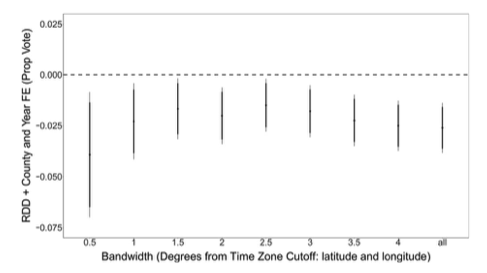
\includegraphics{./imgs/RDD_fig-03.png}

}

\caption{Tamaño del efecto estimado en Schafer y Holbein
(2020)\marginpar{\begin{footnotesize}\leavevmode\vadjust pre{\protect\hypertarget{ref-schafer2020time}{}}%
Schafer, Jerome, y John B Holbein. 2020. {«When time is of the essence:
A natural experiment on how time constraints influence elections»}.
\emph{The Journal of Politics} 82 (2): 418-32.\vspace{2mm}\par\end{footnotesize}}
en función del ancho de banda.}

\end{figure}

En nuestro ejemplo de juguete podemos hacer algo parecido, comparar
todas las estimaciones que fuimos haciendo a lo largo del capítulo:

\begin{Shaded}
\begin{Highlighting}[]
\NormalTok{tabla\_results }\OtherTok{\textless{}{-}} \FunctionTok{tibble}\NormalTok{(Método }\OtherTok{=} \FunctionTok{c}\NormalTok{(}\FunctionTok{rep}\NormalTok{(}\StringTok{"Paramétrico"}\NormalTok{, }\DecValTok{3}\NormalTok{), }\FunctionTok{rep}\NormalTok{(}\StringTok{"No paramétrico"}\NormalTok{, }\DecValTok{5}\NormalTok{)),}
                        \AttributeTok{Kernel =} \FunctionTok{c}\NormalTok{(}\FunctionTok{rep}\NormalTok{(}\StringTok{"No pesado"}\NormalTok{,}\DecValTok{3}\NormalTok{), }\FunctionTok{rep}\NormalTok{(}\StringTok{"Triangular"}\NormalTok{,}\DecValTok{3}\NormalTok{), }\StringTok{"Epanechnikov"}\NormalTok{, }\StringTok{"Uniforme"}\NormalTok{),}
                        \AttributeTok{BW =} \FunctionTok{c}\NormalTok{(}\StringTok{"Full"}\NormalTok{, }\DecValTok{10}\NormalTok{, }\DecValTok{5}\NormalTok{, }\FunctionTok{round}\NormalTok{(}\FunctionTok{c}\NormalTok{(full}\SpecialCharTok{$}\NormalTok{bws[}\DecValTok{1}\NormalTok{,}\DecValTok{1}\NormalTok{], doble}\SpecialCharTok{$}\NormalTok{bws[}\DecValTok{1}\NormalTok{,}\DecValTok{1}\NormalTok{], mitad}\SpecialCharTok{$}\NormalTok{bws[}\DecValTok{1}\NormalTok{,}\DecValTok{1}\NormalTok{], epanechnikov}\SpecialCharTok{$}\NormalTok{bws[}\DecValTok{1}\NormalTok{,}\DecValTok{1}\NormalTok{], uniforme}\SpecialCharTok{$}\NormalTok{bws[}\DecValTok{1}\NormalTok{,}\DecValTok{1}\NormalTok{]), }\DecValTok{3}\NormalTok{)),}
                        \AttributeTok{Estimate =} \FunctionTok{round}\NormalTok{(}\FunctionTok{c}\NormalTok{(modelo\_lm}\SpecialCharTok{$}\NormalTok{coefficients[}\DecValTok{3}\NormalTok{], model\_bw\_10}\SpecialCharTok{$}\NormalTok{coefficients[}\DecValTok{3}\NormalTok{], model\_bw\_5}\SpecialCharTok{$}\NormalTok{coefficients[}\DecValTok{3}\NormalTok{], }
                                           \SpecialCharTok{{-}}\NormalTok{full}\SpecialCharTok{$}\NormalTok{Estimate[}\DecValTok{1}\NormalTok{], }\SpecialCharTok{{-}}\NormalTok{doble}\SpecialCharTok{$}\NormalTok{Estimate[}\DecValTok{1}\NormalTok{], }\SpecialCharTok{{-}}\NormalTok{mitad}\SpecialCharTok{$}\NormalTok{Estimate[}\DecValTok{1}\NormalTok{], }\SpecialCharTok{{-}}\NormalTok{epanechnikov}\SpecialCharTok{$}\NormalTok{Estimate[}\DecValTok{1}\NormalTok{], }\SpecialCharTok{{-}}\NormalTok{uniforme}\SpecialCharTok{$}\NormalTok{Estimate[}\DecValTok{1}\NormalTok{]), }\DecValTok{3}\NormalTok{))}

\NormalTok{tabla\_results }\SpecialCharTok{|\textgreater{}} 
  \FunctionTok{gt}\NormalTok{() }\SpecialCharTok{|\textgreater{}}
  \FunctionTok{gt\_highlight\_rows}\NormalTok{(}\AttributeTok{rows =} \DecValTok{4}\NormalTok{, }
                    \AttributeTok{fill =} \StringTok{"lightyellow"}\NormalTok{,}
                    \AttributeTok{font\_weight =} \StringTok{"bold"}\NormalTok{)}
\end{Highlighting}
\end{Shaded}

\begin{table}
\fontsize{12.0pt}{14.4pt}\selectfont
\begin{tabular*}{\linewidth}{@{\extracolsep{\fill}}lllr}
\toprule
Método & Kernel & BW & Estimate \\ 
\midrule\addlinespace[2.5pt]
Paramétrico & No pesado & Full & 10.800 \\ 
Paramétrico & No pesado & 10 & 9.273 \\ 
Paramétrico & No pesado & 5 & 9.122 \\ 
{\bfseries \cellcolor[HTML]{rgba(255,255,224,0.8)}{\textcolor[HTML]{000000}{No paramétrico}}} & {\bfseries \cellcolor[HTML]{rgba(255,255,224,0.8)}{\textcolor[HTML]{000000}{Triangular}}} & {\bfseries \cellcolor[HTML]{rgba(255,255,224,0.8)}{\textcolor[HTML]{000000}{9.969}}} & {\bfseries \cellcolor[HTML]{rgba(255,255,224,0.8)}{\textcolor[HTML]{000000}{8.578}}} \\ 
No paramétrico & Triangular & 19.938 & 9.151 \\ 
No paramétrico & Triangular & 4.984 & 8.201 \\ 
No paramétrico & Epanechnikov & 8.201 & 8.389 \\ 
No paramétrico & Uniforme & 7.346 & 8.175 \\ 
\bottomrule
\end{tabular*}
\end{table}

Vemos que, en general, no hay grandes diferencias entre las estimaciones
del efecto. La línea resaltada es tal vez el efecto que elegiría si
tuviera que quedarme con uno, ya que el ancho de banda está elegido
basado en los datos, el ajuste es no paramétrico y el kernel le da más
importancia a los datos cerca del umbral. Pero, como vimos en Schafer y
Holbein
(2020)\marginpar{\begin{footnotesize}\leavevmode\vadjust pre{\protect\hypertarget{ref-schafer2020time}{}}%
Schafer, Jerome, y John B Holbein. 2020. {«When time is of the essence:
A natural experiment on how time constraints influence elections»}.
\emph{The Journal of Politics} 82 (2): 418-32.\vspace{2mm}\par\end{footnotesize}},
tal vez sea una buena idea presentar todas las estimaciones y
discutirlas.

\hypertarget{limitaciones-de-la-regresiuxf3n-discontinua}{%
\section{Limitaciones de la regresión
discontinua}\label{limitaciones-de-la-regresiuxf3n-discontinua}}

La regresión discontinua es una herramienta muy interesante y con mucho
auge en la investigación causal, especialmente cuando tenemos confusores
no observados. Pero, como vimos, requiere de algunas condiciones
particulares para poder aplicarla: tener una \emph{running variable} que
sea continua y que tenga un umbral, y que los sujetos a uno y otro lado
del umbral sean comparables (ya vamos a hablar un poco de esto). En esta
sección vamos a nombrar brevemente tres de las pincipales limitacinoes
de la regresión discontinua.

\hypertarget{es-data-greedy}{%
\subsection{\texorpdfstring{Es \emph{data
greedy}}{Es data greedy}}\label{es-data-greedy}}

Una de las principales limitaciones de la regresión discontinua es que
requiere una gran cantidad de datos para poder estimar el efecto causal.
Esto se debe a que los sujetos que son comparables para una estimación
confiables del \textbf{LATE} son aquellos que están cerca del umbral.
Por lo tanto, nuestra muestra puede ser grande, pero una vez que fijamos
el ancho de banda se puede reducir notablemente.

\hypertarget{es-limitada-en-alcance}{%
\subsection{Es limitada en alcance}\label{es-limitada-en-alcance}}

Otra limitación de la regresión discontinua es que el efecto estimado es
local, es decir, sólo es válido para los sujetos que están cerca del
umbral. Esto significa que no debemos generalizar esta estimación a toda
la población, es decir, tenemos un problema de validez externa. Esto
podría ser un problema ya que normalmente queremos estimar el efecto
para la población de interés.

Acá cabe una breve reflexión: ¿No son todos los efectos que calculamos
de algún modo locales? Entonces, resulta interesante pensar cuáles son
las condiciones necesarias para que el \textbf{LATE} estimado sea
generalizable. Por ejemplo: ¿Creen que el ejemplo del padrón electoral
es generalizable? Cada problema se enfrenta con esa pregunta y cada
respuesta requiere de un conocimiento del dominio y de la muestra con la
que se está trabajando para responderla.

\hypertarget{puede-haber-problemas-de-manipulaciuxf3n}{%
\subsection{\texorpdfstring{Puede haber problemas de
\textbf{manipulación}}{Puede haber problemas de manipulación}}\label{puede-haber-problemas-de-manipulaciuxf3n}}

Recordemos algo: Al asumir que los participantes de un lado y del otro
de la discontinuidad son comparables, estamos asumiendo que hay
continuidad en la esperanza de los \emph{potential outcomes}, es decir,
que si un sujeto estuviera en el grupo tratamiento tendría en el umbral
el mismo \emph{outcome} que tendría un miembro del grupo control si
hubiera sido asignado al tratamiento. Es un trabalenguas, ¿no? Veamos
primero las cuentas y pensemos después en un ejemplo.

Con continuidad de los \emph{potential outcomes} nos referimos a que los
\emph{potential outcomes} no cambian abruptamente en el umbral, es
decir, que la esperanza de los \emph{potential outcomes} es continua en
el umbral. En difícil: que \(E[Y_i^1]\) y \(E[Y_i^0]\) son continuas en
el umbral. En términos de la \emph{running variable} \(X\) y siendo su
umbral \(c\), esto significa que:

\[
\begin{align*}
\lim_{x \to c^-} E[Y_i^1] = \lim_{x \to c^+} E[Y_i^1] \\
\lim_{x \to c^-} E[Y_i^0] = \lim_{x \to c^+} E[Y_i^0]
\end{align*}
\]

O gráficamente:

\begin{Shaded}
\begin{Highlighting}[]
\FunctionTok{set.seed}\NormalTok{(}\DecValTok{123}\NormalTok{)}
\NormalTok{data }\OtherTok{\textless{}{-}} \FunctionTok{tibble}\NormalTok{(}\AttributeTok{x =} \FunctionTok{runif}\NormalTok{(}\DecValTok{200}\NormalTok{, }\SpecialCharTok{{-}}\DecValTok{10}\NormalTok{, }\DecValTok{10}\NormalTok{),}
               \AttributeTok{y =}\NormalTok{ x }\SpecialCharTok{+} \FunctionTok{c}\NormalTok{(}\FunctionTok{rnorm}\NormalTok{(}\DecValTok{100}\NormalTok{, }\AttributeTok{mean =} \DecValTok{5}\NormalTok{, }\AttributeTok{sd =} \DecValTok{2}\NormalTok{), }
                     \FunctionTok{rnorm}\NormalTok{(}\DecValTok{100}\NormalTok{, }\AttributeTok{mean =} \DecValTok{0}\NormalTok{, }\AttributeTok{sd =} \DecValTok{2}\NormalTok{)),}
               \AttributeTok{outcome =} \FunctionTok{c}\NormalTok{(}\FunctionTok{rep}\NormalTok{(}\StringTok{"Y1"}\NormalTok{, }\DecValTok{100}\NormalTok{), }\FunctionTok{rep}\NormalTok{(}\StringTok{"Y0"}\NormalTok{, }\DecValTok{100}\NormalTok{))) }\SpecialCharTok{\%\textgreater{}\%}
  \FunctionTok{mutate}\NormalTok{(}\AttributeTok{status =} \FunctionTok{if\_else}\NormalTok{((outcome }\SpecialCharTok{==} \StringTok{"Y1"} \SpecialCharTok{\&}\NormalTok{ x}\SpecialCharTok{\textgreater{}}\DecValTok{0}\NormalTok{) }\SpecialCharTok{|}\NormalTok{ (outcome }\SpecialCharTok{==} \StringTok{"Y0"} \SpecialCharTok{\&}\NormalTok{ x}\SpecialCharTok{\textless{}=}\DecValTok{0}\NormalTok{), }
                          \StringTok{"Observable"}\NormalTok{, }\StringTok{"Contrafáctico"}\NormalTok{))}

\NormalTok{lines }\OtherTok{\textless{}{-}} \FunctionTok{tibble}\NormalTok{(}\AttributeTok{intercept =} \FunctionTok{c}\NormalTok{(}\DecValTok{5}\NormalTok{, }\DecValTok{0}\NormalTok{),}
                \AttributeTok{slope =} \FunctionTok{c}\NormalTok{(}\DecValTok{1}\NormalTok{, }\DecValTok{1}\NormalTok{),}
                \AttributeTok{outcome =} \FunctionTok{c}\NormalTok{(}\StringTok{"Y1"}\NormalTok{, }\StringTok{"Y0"}\NormalTok{))}

\FunctionTok{ggplot}\NormalTok{(data, }\FunctionTok{aes}\NormalTok{(}\AttributeTok{x =}\NormalTok{ x, }\AttributeTok{y =}\NormalTok{ y, }\AttributeTok{color =}\NormalTok{ outcome)) }\SpecialCharTok{+}
  \FunctionTok{geom\_point}\NormalTok{(}\FunctionTok{aes}\NormalTok{(}\AttributeTok{alpha =}\NormalTok{ status), }\AttributeTok{size =} \DecValTok{2}\NormalTok{) }\SpecialCharTok{+}
  \FunctionTok{geom\_vline}\NormalTok{(}\AttributeTok{xintercept =} \DecValTok{0}\NormalTok{, }\AttributeTok{linetype =} \StringTok{"dashed"}\NormalTok{, }\AttributeTok{color =} \StringTok{"darkblue"}\NormalTok{) }\SpecialCharTok{+}
  \FunctionTok{geom\_abline}\NormalTok{(}\AttributeTok{data =}\NormalTok{ lines, }\FunctionTok{aes}\NormalTok{(}\AttributeTok{slope =}\NormalTok{ slope, }\AttributeTok{intercept =}\NormalTok{ intercept, }\AttributeTok{color =}\NormalTok{ outcome), }\AttributeTok{linewidth =} \DecValTok{1}\NormalTok{) }\SpecialCharTok{+}
  \FunctionTok{labs}\NormalTok{(}\AttributeTok{x =} \StringTok{"Running variable (X)"}\NormalTok{, }
       \AttributeTok{y =} \StringTok{"Potential outcomes (Y)"}\NormalTok{,}
       \AttributeTok{color =} \ConstantTok{NULL}\NormalTok{,}
       \AttributeTok{alpha =} \ConstantTok{NULL}\NormalTok{) }\SpecialCharTok{+}
  \FunctionTok{scale\_color\_brewer}\NormalTok{(}\AttributeTok{palette =} \StringTok{"Dark2"}\NormalTok{) }\SpecialCharTok{+}
  \FunctionTok{scale\_alpha\_manual}\NormalTok{(}\AttributeTok{values =} \FunctionTok{c}\NormalTok{(.}\DecValTok{2}\NormalTok{, }\DecValTok{1}\NormalTok{)) }\SpecialCharTok{+}
  \FunctionTok{theme\_minimal}\NormalTok{() }\SpecialCharTok{+}
  \FunctionTok{theme}\NormalTok{(}\AttributeTok{legend.position =} \StringTok{"top"}\NormalTok{, }\AttributeTok{legend.box=}\StringTok{"vertical"}\NormalTok{)}
\end{Highlighting}
\end{Shaded}

\begin{figure}[H]

{\centering 
\includegraphics[width=18.75in,height=\textheight]{./reg_discontinua_files/figure-pdf/unnamed-chunk-21-1.pdf}

}

\caption{Continuidad de los potential outcomes en el umbral.}

\end{figure}

En esta figura vemos como puntos llenos a los observables y como puntos
grisados a los contrafácticos, las líneas, son las esperanzas de estos
\emph{outcomes}. Lo que nos interesa pensar es que, si bien en los datos
observados vemos un salto al cruzar el umbral (es decir, al pasar de no
estar expuesto a estar expuesto al tratamiento), si pudiéramos observar
los \emph{potential outcomes} al cruzar el umbral veríamos que son
continuos. Es decir, que si un sujeto estuviera en el grupo tratamiento
tendría en el umbral el mismo \emph{outcome} que que tendría un miembro
del grupo control si hubiera sido asignado al tratamiento.

Pensemos qué implicancias tiene esto. Esto significa que la
\emph{running variable} no puede ser manipulada por los sujetos. Es
decir, que los sujetos no pueden elegir estar a un lado o del otro del
umbral. Por ejemplo, si por algún motivo en nuestro ejemplo los alumnos
conocieran la regla de selección y se sacaran peor nota para tener una
tutoría gratuita, en ese caso estaríamos hablando de
\textbf{manipulación} y la estimación del efecto del tratamiento estaría
sesgada.

Vamos con un ejemplo bien concreto. Imaginemos que queremos evaluar la
política pública de la que hablamos al principio del capítulo, esa a la
que uno califica por cobrar menos de \$\(350000\) mensuales. Imaginen
que soy un cuentapropista que tengo ese beneficio y a dos días de
terminar el mes ya facturé \$\(349999\). De golpe me llaman para
ofrecerme un trabajo de \$\(500\), ¿qué creen que voy a decir? Bueno, si
la política es lo suficientemente beneficiosa (más que \$\(499\))
probablemente voy a decir que no. ¿Por qué? Porque si acepto el trabajo,
voy a perder el beneficio de la política pública. Entonces, en este
caso, la \emph{running variable} (mi ingreso mensual) fue manipulado y,
por lo tanto, la continuidad de los \emph{potential outcomes} no se
cumple. Sé que es un ejemplo un poco irreal, pero tómense el tiempo de
pensar cuántas veces podemos ver este tipo de manipulación en la vida
real.

Existen diversas formas de detectar la manipulación en los datos. Una de
las más comunes es la de observar la densidad de la \emph{running
variable} alrededor del umbral. Si hay manipulación, deberíamos ver un
salto en la densidad de la \emph{running variable} en el umbral. Esto se
debe a que los sujetos que están cerca del umbral son los que tienen más
probabilidades de ser manipulados. Existe algo llamado test de densidad
de McCrary que sirve para verificar esto (McCrary
(2008)\marginpar{\begin{footnotesize}\leavevmode\vadjust pre{\protect\hypertarget{ref-mccrary2008manipulation}{}}%
McCrary, Justin. 2008. {«Manipulation of the running variable in the
regression discontinuity design: A density test»}. \emph{Journal of
econometrics} 142 (2): 698-714.\vspace{2mm}\par\end{footnotesize}}),
pero no vamos a entrar en demasiado detalle. Este test está implementado
en la función \texttt{rddensity()} del paquete \texttt{rddensity}.

Veamos cómo se ve la densidad de la \emph{running variable} en nuestro
ejemplo de las tutorías (utilizando las funciones \texttt{rddensity} y
\texttt{rdplotdensity}).

\begin{Shaded}
\begin{Highlighting}[]
\NormalTok{test\_density }\OtherTok{\textless{}{-}} \FunctionTok{rddensity}\NormalTok{(tutoring}\SpecialCharTok{$}\NormalTok{entrance\_exam, }\AttributeTok{c =} \DecValTok{70}\NormalTok{)}
\NormalTok{plot\_density\_test }\OtherTok{\textless{}{-}} \FunctionTok{rdplotdensity}\NormalTok{(}\AttributeTok{rdd =}\NormalTok{ test\_density, }
                                   \AttributeTok{X =}\NormalTok{ tutoring}\SpecialCharTok{$}\NormalTok{entrance\_exam, }
                                   \AttributeTok{type =} \StringTok{"both"}\NormalTok{)}
\end{Highlighting}
\end{Shaded}

\begin{figure}[H]

{\centering 
\includegraphics[width=18.75in,height=\textheight]{./reg_discontinua_files/figure-pdf/unnamed-chunk-22-1.pdf}

}

\caption{Testeamos la posible manipulación en el ejemplo de las
tutorías.}

\end{figure}

Es razonable decir que no hay manipulación ¿no?

\bookmarksetup{startatroot}

\hypertarget{sec-var-inst}{%
\chapter{Variables instrumentales}\label{sec-var-inst}}

\begin{tcolorbox}[enhanced jigsaw, breakable, colback=white, rightrule=.15mm, opacityback=0, colframe=quarto-callout-warning-color-frame, bottomrule=.15mm, left=2mm, toprule=.15mm, leftrule=.75mm, arc=.35mm]
\begin{minipage}[t]{5.5mm}
\textcolor{quarto-callout-warning-color}{\faExclamationTriangle}
\end{minipage}%
\begin{minipage}[t]{\textwidth - 5.5mm}
Este capítulo se encuentra en construcción 🏗.\end{minipage}%
\end{tcolorbox}

\bookmarksetup{startatroot}

\hypertarget{referencias}{%
\chapter*{Referencias}\label{referencias}}
\addcontentsline{toc}{chapter}{Referencias}




\end{document}
